\documentclass[UTF8,12pt,a4paper,oneside]{ctexbook}
\usepackage[margin=25mm]{geometry}
\usepackage{fontspec}
\setmainfont{Times New Roman}
\setsansfont{Times New Roman}
\setmonofont{DejaVu Sans Mono}
\setCJKmainfont[
  BoldFont=FandolSong-Bold.otf,
  ItalicFont=FandolKai-Regular.otf
]{FandolSong-Regular.otf}
\setCJKsansfont[
  BoldFont=FandolHei-Bold.otf
]{FandolHei-Regular.otf}
\setCJKmonofont[
  BoldFont=FandolHei-Bold.otf
]{FandolHei-Regular.otf}
\usepackage{amsmath,amssymb,mathtools}
\usepackage{unicode-math}
\setmathfont{TeX Gyre Termes Math}
\usepackage{newunicodechar}
\newunicodechar{∅}{\ensuremath{\varnothing}}
\newunicodechar{ℰ}{\ensuremath{\mathcal{E}}}
\newunicodechar{ℜ}{\ensuremath{\mathfrak{R}}}
\newunicodechar{⊗}{\ensuremath{\otimes}}
\newunicodechar{∈}{\ensuremath{\in}}
\newunicodechar{∘}{\ensuremath{\circ}}
\newunicodechar{↦}{\ensuremath{\mapsto}}
\newunicodechar{∇}{\ensuremath{\nabla}}
\newunicodechar{⇒}{\ensuremath{\Rightarrow}}
\newunicodechar{∨}{\ensuremath{\vee}}
\newunicodechar{∪}{\ensuremath{\cup}}
\newunicodechar{⊕}{\ensuremath{\oplus}}
\newunicodechar{⇔}{\ensuremath{\Leftrightarrow}}
\newunicodechar{⊂}{\ensuremath{\subset}}
\newunicodechar{∧}{\ensuremath{\wedge}}
\newunicodechar{⊤}{\ensuremath{\top}}
\usepackage{graphicx}
\usepackage{longtable,booktabs,array}
\usepackage{xcolor,framed,fancyvrb}
\usepackage{setspace}
\usepackage{enumitem}
\usepackage{microtype}
\usepackage[hidelinks,unicode,pdfusetitle,bookmarksnumbered]{hyperref}
\usepackage[open,openlevel=2]{bookmark}
\doublespacing
\setlength{\parindent}{1.5em}
\setlength{\parskip}{0pt}
\setcounter{tocdepth}{2}
\setcounter{secnumdepth}{2}
\setlist{itemsep=0.25\baselineskip,topsep=0.25\baselineskip}
\providecommand{\tightlist}{\setlength{\itemsep}{0pt}\setlength{\parskip}{0pt}}
\providecommand{\pandocbounded}[1]{#1}
\newcommand{\specialchapter}[1]{%
  \chapter*{#1}%
  \phantomsection
  \addcontentsline{toc}{chapter}{#1}%
}
\newcounter{exercisesection}
\newcommand{\exercisesection}[1]{%
  \refstepcounter{exercisesection}%
  \section*{第\theexercisesection 节习题：#1}%
  \phantomsection
  \addcontentsline{toc}{section}{第\theexercisesection 节习题：#1}%
}
\definecolor{shadecolor}{RGB}{248,248,248}
\newenvironment{Shaded}{\begin{snugshade}}{\end{snugshade}}
\newenvironment{Highlighting}[1][]{}{}
\newcommand{\NormalTok}[1]{#1\par}
\makeatletter
\def\maxwidth{\ifdim\Gin@nat@width>\linewidth\linewidth\else\Gin@nat@width\fi}
\def\maxheight{\ifdim\Gin@nat@height>0.8\textheight 0.8\textheight\else\Gin@nat@height\fi}
\makeatother
\setkeys{Gin}{width=\maxwidth,height=\maxheight,keepaspectratio}
\graphicspath{{images/}}
\emergencystretch=3em
\pagestyle{plain}
\title{代数学（第10章）}
\author{尼古拉·布尔巴基}
\date{}
\begin{document}
\pagenumbering{gobble}
\maketitle
\clearpage
\frontmatter
\tableofcontents
\mainmatter
\setcounter{chapter}{9}
\chapter{同调代数}

\section{线性代数的补充}

在本节中，字母 A 表示一个环。除非另有明确说明，所考虑的所有模均为左模，所有理想均为左理想。

这些定义和结果适用于右模，只需将它们视为相反环上的左模即可。

如果 M 是一个 A-模，并且如果 \(a \in A\) ，我们用 \(a_{M}\) 表示 M 的位似 \(x \mapsto ax\) 。因此我们有 \(1_{M} = Id_{M}\) （M 的恒等映射）；当不会产生混淆时，有时简写为 1 来代替 \(1_{M}\) .

最后，我们用 0 表示一个化为其单位元的 A-模，该模一经选定便固定下来（参见 II，第 8 页）。

\subsection{交换图}

设，例如，B、C、D、E、F 为五个集合，并设 \(f\) 是从 E 到 F 的映射， \(g\) 是从 B 到 C 的映射， \(h\) 是从 D 到 E 的映射， \(u\) 是从 B 到 D 的映射，且 \(v\) 是从C到E的一个映射。为了概括这类情形，人们常借助图表；例如，前述情形可用下图（E，II，第14页）来概括：

\[
\begin{array}{c} \mathrm{B} \xrightarrow {g} \mathrm{C} \\ u \Big \downarrow \\ \mathrm{D} \xrightarrow [ h ]{} \mathrm{E} \xrightarrow [ f ]{} \mathrm{F}. \end{array}\tag{1}
\]

在这样的图中，符号组 E \(\xrightarrow{f}\) F 示意了 f 是从 E 到 F 的映射这一事实。当对 f 不存在歧义时，可省略字母 f，直接写作 E \(\rightarrow\) F.

当B、C、D、E、F是群（相应地，A-模）且f、g、h、u、v是群（相应地，A-模）的同态时，为简洁起见，称图(1)为群（相应地，A-模）的图。

原则上，图不是数学对象，而仅仅是一个图形，旨在便于阅读证明。在实践中，人们常将图用作缩写符号，以避免逐一命名所有要考虑的集合和映射；因此，人们说“考虑图(1)”，而不是说：“设B、C、D、E、F为五个集合\ldots{} 且v为从C到E的映射”；例如参见第2节命题1的陈述。

例如，考虑下面的图表：

\[
\begin{array}{c} \mathrm{B} \xrightarrow {f} \mathrm{C} \xrightarrow {g} \mathrm{D} \xrightarrow {h} \mathrm{E} \\ b \Big \downarrow \qquad \qquad c \Big \downarrow \qquad \qquad d \Big \downarrow \qquad e \Big \downarrow \\ \mathrm{B} ^ {\prime} \xrightarrow {f ^ {\prime}} \mathrm{C} ^ {\prime} \xrightarrow {g ^ {\prime}} \mathrm{D} ^ {\prime} \xrightarrow {h ^ {\prime}} \mathrm{E} ^ {\prime}. \end{array}\tag{2}
\]

对于由图中若干段按箭头所示方向经过的线段组成的每条路径，都对应一个从第一段起点所表示集合到末段终点所表示集合的映射，即所经过各段对应映射的复合。对于图中的每个顶点，例如C，约定存在一条仅由C构成的路径，并约定与之对应恒等映射 1 \(_{C}\) .

在（2）中，例如，有三条从B出发、终止于D'的路径；相应的映射为 \(d \circ g \circ f\) , \(g' \circ c \circ f\) 和 \(g' \circ f' \circ b\) 。我们说一个图表是交换的，如果对于图表中具有相同起点和相同终点的每一对路径，对应的两个映射相等；特别地，如果一条路径的终点与其起点重合，则对应的映射必须是恒等映射。

为使图（2）可交换，其充要条件是以下关系式

\[
f ^ {\prime} \circ b = c \circ f, \qquad g ^ {\prime} \circ c = d \circ g, \qquad h ^ {\prime} \circ d = e \circ h;\tag{3}
\]

保持；换言之，从（2）中提取的三个方形图可交换是必要且充分的。事实上，关系式（3）蕴含 \(d \circ g \circ f = g' \circ c \circ f\) 因为 \(d \circ g = g' \circ c\) ，以及 \(g' \circ c \circ f = g' \circ f' \circ b\) ，因为 \(c \circ f = f' \circ b\) 因此，从B出发并以D'结束的三条路径给出相同的映射。类似地可以验证，从B出发并以E'结束的四条路径（分别地，从C出发并以E'结束的三条路径）给出相同的映射。关系式(3)意味着从B（分别地，C、D）出发并以C'（分别地，D'、E'）结束的两条路径给出相同的映射。(2)中所有其他顶点对至多由一条路径连接，因此图(2)确实是可交换的。

在下文中，我们将把对其他类型图表进行类似结果的表述与验证这一任务留给读者。

\subsection{蛇形图}

命题 1. --- 考虑一个 A-模的交换图

\[
\begin{array}{c} \mathrm{M} \xrightarrow {u} \mathrm{N} \xrightarrow {v} \mathrm{P} \\ f \Big \downarrow \qquad \qquad \qquad g \Big \downarrow \qquad \qquad \qquad h \Big \downarrow \\ \mathrm{M} ^ {\prime} \xrightarrow {u ^ {\prime}} \mathrm{N} ^ {\prime} \xrightarrow {v ^ {\prime}} \mathrm{P} ^ {\prime}. \end{array}\tag{4}
\]

假设 (4) 的两行是正合的。则：

\begin{enumerate}
\def\labelenumi{(\roman{enumi})}
\tightlist
\item
  若 h 是单射，我们有
\end{enumerate}

\[
\operatorname{Im} (g) \cap \operatorname{Im} \left(u ^ {\prime}\right) = \operatorname{Im} \left(u ^ {\prime} \circ f\right) = \operatorname{Im} (g \circ u).\tag{5}
\]

\begin{enumerate}
\def\labelenumi{(\roman{enumi})}
\setcounter{enumi}{1}
\tightlist
\item
  若 f 是满射，我们有
\end{enumerate}

\[
\operatorname{Ker} (g) + \operatorname{Im} (u) = \operatorname{Ker} \left(v ^ {\prime} \circ g\right) = \operatorname{Ker} (h \circ v).\tag{6}
\]

让我们证明 (i)。显然我们有

\[
\operatorname{Im} \left(u ^ {\prime} \circ f\right) = \operatorname{Im} (g \circ u) \subset \operatorname{Im} (g) \cap \operatorname{Im} \left(u ^ {\prime}\right).
\]

反之，设 \(y' \in \operatorname{Im}(g) \cap \operatorname{Im}(u')\) 。存在 \(y \in \mathbf{N}\) 使得 \(y' = g(y)\) 。由于 \(v' \circ u' = 0\) ，我们有 \(0 = v'(y') = v'(g(y)) = h(v(y))\) ，从而 \(v(y) = 0\) ，因为 \(h\) 是单射。由于 \((u, v)\) 是正合序列，存在 \(x \in \mathbf{M}\) 使得 \(y = u(x)\) ，从而 \(y' = g(u(x))\) .

让我们证明 (ii)。由于 \(v \circ u = 0\) 且 \(v' \circ u' = 0\) ，显然

\[
\operatorname{Ker} (g) + \operatorname{Im} (u) \subset \operatorname{Ker} \left(v ^ {\prime} \circ g\right) = \operatorname{Ker} (h \circ v).
\]

反之，设 \(y \in \operatorname{Ker}(v' \circ g)\) 。然后 \(g(y) \in \operatorname{Ker}(v')\) ，并且存在 \(x' \in M'\) 使得 \(u'(x') = g(y)\) 由于序列 \((u', v')\) 是正合的。由于 \(f\) 是满射的，存在 \(x \in M\) 使得 \(f(x) = x'\) ，从而 \(g(y) = u'(f(x)) = g(u(x))\) ；由此我们得出结论 \(y - u(x) \in \operatorname{Ker}(g)\) ，这就完成了证明。

引理1. —— 考虑一个A-模的交换图

\[
\begin{array}{c} \mathbf {M} \xrightarrow {\quad u \quad} \mathbf {N} \\ f \Big \downarrow \qquad \qquad \qquad \qquad \qquad \qquad \qquad \qquad g \Big \downarrow \\ \mathbf {M} ^ {\prime} \xrightarrow {\quad u ^ {\prime} \quad} \mathbf {N} ^ {\prime}. \end{array}\tag{7}
\]

那么存在唯一的同态 \(u_1: \text{Ker}(f) \to \text{Ker}(g)\) 和唯一的同态 \(u_2: \text{Coker}(f) \to \text{Coker}(g)\) ，使得以下图表

\[
\begin{array}{c} \operatorname{Ker} (f) \xrightarrow {u _ {1}} \operatorname{Ker} (g) \\ i \Biggl \downarrow \\ \mathrm{M} \xrightarrow [ u ]{} \mathrm{N} \end{array}\tag{8}
\]

和

\begin{enumerate}
\def\labelenumi{(\arabic{enumi})}
\setcounter{enumi}{8}
\tightlist
\item
\end{enumerate}

\pandocbounded{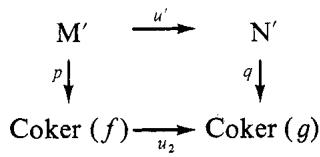
\includegraphics[keepaspectratio]{images/part001_11db974a.jpg}}

设它们是交换的，其中i和j表示典范单射，p和q表示典范满射。

事实上，若 \(x \in \operatorname{Ker}(f)\) ，我们有 \(f(x) = 0\) 和 \(g(u(x)) = u'(f(x)) = 0\) ，因此 \(u(x) \in \operatorname{Ker}(g)\) ，于是 \(u_1\) 的存在性与唯一性立即得出。同样地，我们有

\[
u ^ {\prime} (f (\mathbf {M})) = g (u (\mathbf {M})) \subset g (\mathbf {N}),
\]

因此 \(u'\) 通过取商给出一个同态

\[
u _ {2}: \operatorname{Coker} (f) \rightarrow \operatorname{Coker} (g),
\]

这是使（9）可交换的唯一同态。

现在从A-模的交换图（4）出发；根据引理1，它对应一个交换图

\[
\begin{array}{c c c c c} \operatorname{Ker} (f) \xrightarrow {u _ {1}} & \operatorname{Ker} (g) \xrightarrow {v _ {1}} & \operatorname{Ker} (h) \\ i \Big \downarrow & j \Big \downarrow & k \Big \downarrow \\ \mathbf {M} & u & \mathbf {N} & v & \mathbf {P} \\ f \Big \downarrow & g \Big \downarrow & h \Big \downarrow \\ \mathbf {M} ^ {\prime} & u ^ {\prime} & \mathbf {N} ^ {\prime} & v ^ {\prime} & \mathbf {P} ^ {\prime} \\ p \Big \downarrow & q \Big \downarrow & r \Big \downarrow \\ \operatorname{Coker} (f) \xrightarrow {u _ {2}} & \operatorname{Coker} (g) \xrightarrow {v _ {2}} & \operatorname{Coker} (h) \end{array}\tag{10}
\]

其中 \(i, j, k\) 是典范单射， \(p, q, r\) 是典范满射， \(u_{1}, u_{2}\) （相应地， \(v_{1}, v_{2}\) ）是由 \(u\) , \(u'\) （相应地， \(v, v'\) ）依引理1得出的同态。

命题2. --- 假设在交换图 (4) 中，序列 \((u, v)\) 与 \((u', v')\) 是正合的。则：

\begin{enumerate}
\def\labelenumi{(\roman{enumi})}
\item
  我们有 \(v_{1} \circ u_{1} = 0\) ；若 \(u'\) 是单射的，则序列 \((u_{1}, v_{1})\) 是正合的。
\item
  我们有 \(v_2 \circ u_2 = 0\) ；若v是满射，则序列 \((u_2, v_2)\) 是正合的。
\item
  假设 \(u'\) 是单射且 \(v\) 是满射。则存在且仅存在一个同态 \(d: \operatorname{Ker}(h) \to \operatorname{Coker}(f)\) 具有以下性质：如果 \(z \in \operatorname{Ker}(h)\) , \(y \in \mathbf{N}\) 与 \(x' \in \mathbf{M}'\) 满足关系 \(v(y) = k(z)\) 和 \(u'(x') = g(y)\) ，我们有 \(d(z) = p(x')\) 。此外，序列
\end{enumerate}

(*) \(\operatorname{Ker}(f) \xrightarrow{u_1} \operatorname{Ker}(g) \xrightarrow{v_1} \operatorname{Ker}(h) \xrightarrow{d} \operatorname{Coker}(f) \xrightarrow{u_2} \operatorname{Coker}(g) \xrightarrow{v_2} \operatorname{Coker}(h)\) 是正合的。

\pandocbounded{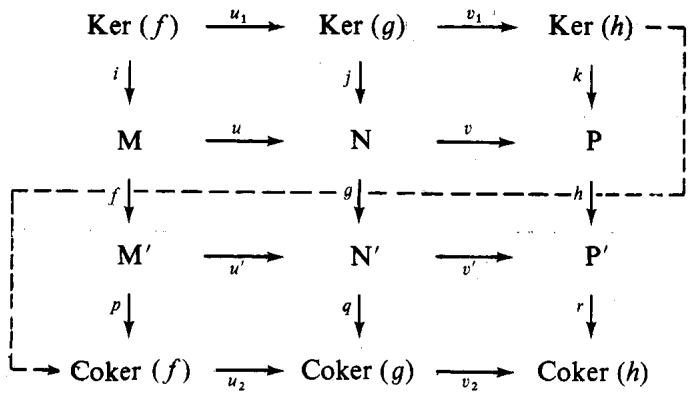
\includegraphics[keepaspectratio]{images/part001_0570902c.jpg}}

让我们证明 (i)。因为 \(u_{1}\) 与 \(v_{1}\) 分别同 \(u\) 和 \(v\) 到 \(\operatorname{Ker}(f)\) 与 \(\operatorname{Ker}(g)\) 上的限制具有相同的图像，我们有 \(v_{1} \circ u_{1} = 0\) 。我们有

\[
\operatorname{Ker} \left(v _ {1}\right) = \operatorname{Ker} (g) \cap \operatorname{Ker} (v) = \operatorname{Ker} (g) \cap \operatorname{Im} (u) = \operatorname{Im} (j) \cap \operatorname{Im} (u).
\]

但由命题1(i)，我们有 \(\operatorname{Ker}(v_1) = \operatorname{Im}(j \circ u_1) = \operatorname{Im}(u_1)\) 如果 \(u'\) 是单射。我们来证明 (ii)。由于 \(u_2\) 与 \(v_2\) 是由 \(u\) 和 \(v\) 通过取商得出的，显然 \(v_2 \circ u_2 = 0\) 。假设 \(v\) 是满射；由于 \(q\) 与 \(p\) 是满射，根据假设及命题 1 (ii)，我们有

\[
\begin{array}{r l} \operatorname{Ker} (v _ {2}) & = q (\operatorname{Ker} (v _ {2} \circ q)) = q (\operatorname{Ker} (v ^ {\prime}) + \operatorname{Im} (g)) = q (\operatorname{Ker} (v ^ {\prime})) \\ & = q (\operatorname{Im} (u ^ {\prime})) = \operatorname{Im} (q \circ u ^ {\prime}) = \operatorname{Im} (u _ {2} \circ p) = \operatorname{Im} (u _ {2}). \end{array}
\]

最后，我们来证明（iii）。对于 \(z \in \operatorname{Ker}(h)\) 存在 \(y \in \mathbf{N}\) 使得 \(v(y) = k(z)\) 因为 \(v\) 是满射；此外，我们有 \(v'(g(y)) = h(k(z)) = 0\) 因此存在唯一的 \(x' \in \mathbf{M}'\) 使得 \(u'(x') = g(y)\) 因为 \(u'\) 是单射。让我们证明元素 \(p(x') \in \operatorname{Coker}(f)\) 不依赖于元素 \(y \in \mathbf{N}\) ，只要它满足 \(v(y) = k(z)\) 。事实上，如果 \(y_1 \in \mathbf{N}\) 是另一个满足 \(v(y_1) = k(z)\) 的元素，我们有 \(y_1 = y + u(x)\) ，其中 \(x \in \mathbf{M}\) 。让我们证明，如果 \(x_1' \in \mathbf{M}'\) 满足 \(u'(x_1') = g(y_1)\) ，则 \(x_1' = x' + f(x)\) ；事实上，我们有 \(u'(x' + f(x)) = u'(x') + u'(f(x)) = g(y) + g(u(x)) = g(y + u(x)) = g(y_1)\) 最后，我们得出结论 \(p(x_1') = p(x') + p(f(x)) = p(x')\) 。因此我们可令 \(d(z) = p(x')\) ，并由此定义了一个映射 \(d: \operatorname{Ker}(h) \to \operatorname{Coker}(f)\) 。

如果现在 \(z_{1}, z_{2}\) 是 \(\operatorname{Ker}(h)\) 的元素，如果 \(\lambda_{1}, \lambda_{2} \in \mathbf{A}\) 和 \(z = \lambda_{1} z_{1} + \lambda_{2} z_{2}\) ，我们取元素 \(y_{1}\) 和 \(y_{2}\) 属于 \(\mathbf{N}\) ，使得 \(v(y_{1}) = k(z_{1})\) 和 \(v(y_{2}) = k(z_{2})\) ，并为 \(y \in \mathbf{N}\) 选取元素 \(\lambda_{1} y_{1} + \lambda_{2} y_{2}\) ；那么立即可以得出

\[
d (z) = \lambda_ {1} d (z _ {1}) + \lambda_ {2} d (z _ {2}),
\]

所以 d 是一个同态。

假设 \(z = v_1(t)\) 对于某个 \(t \in \operatorname{Ker}(g)\) ；我们将取 \(y \in \mathbf{N}\) 为元素 \(j(t)\) 。由于 \(g(j(t)) = 0\) ，我们得出结论 \(d(z) = 0\) ，因此 \(d \circ v_1 = 0\) 。反之，假设 \(d(z) = 0\) 。利用前面的记号，我们因此有 \(x' = f(x)\) ，其中 \(x \in M\) 。在这种情况下，我们有 \(g(y) = u'(f(x)) = g(u(x))\) ，或等价地 \(g(y - u(x)) = 0\) 。元素 \(y - u(x)\) 因此具有形式 \(j(n)\) 当 \(n \in \operatorname{Ker}(g)\) ，并且我们有

\[
k (z) = v (y) = v (u (x) + j (n)) = v (j (n)) = k \left(v _ {1} (n)\right);
\]

因为 \(k\) 是单射， \(z = v_{1}(n)\) ，这证明了序列(*)在 \(\operatorname{Ker}(h)\) 处是正合的。最后，我们仍有（使用相同的记号）

\[
u _ {2} (d (z)) = u _ {2} \left(p \left(x ^ {\prime}\right)\right) = q \left(u ^ {\prime} \left(x ^ {\prime}\right)\right) = q (g (y)) = 0 \quad \text {   hence   } \quad u _ {2} \circ d = 0.
\]

反之，假设一个元素 \(w = p(x')\) —— Coker \((f)\) 的元素 —— 满足

\[
u _ {2} (w) = u _ {2} \left(p \left(x ^ {\prime}\right)\right) = 0 \quad \left(\operatorname{with} x ^ {\prime} \in \mathbf {M} ^ {\prime}\right).
\]

我们因此有 \(q(u'(x')) = 0\) ，从而 \(u'(x') = g(y)\) 对于某个 \(y \in \mathbb{N}\) ；由于 \(v'(u'(x')) = 0\) ，我们有 \(v'(g(y)) = 0\) ，因此 \(h(v(y)) = 0\) ，换言之 \(v(y) = k(z)\) 对于某个 \(z \in \operatorname{Ker}(h)\) ，并且根据定义 \(w = d(z)\) ，这表明序列(*)在Coker( \(f\) )处是正合的。我们在(i)中看到它在Ker( \(g\) )处是正合的，在(ii)中看到它在Coker( \(g\) )处是正合的，这完成了(iii)的证明。

推论1. --- 假设图(4)是交换的且具有正合的行。则：

\begin{enumerate}
\def\labelenumi{(\roman{enumi})}
\item
  若 \(u'\) , \(f\) 和 \(h\) 是单射，则 \(g\) 是单射。
\item
  如果v、f和h是满射，则g是满射。
\end{enumerate}

断言 (i) 由命题 2 的断言 (i) 得出：事实上，我们有 \(\operatorname{Ker}(f) = 0\) 和 \(\operatorname{Ker}(h) = 0\) ，因此 \(\operatorname{Ker}(g) = 0\) 。

断言(ii)由命题2的断言(ii)得出：事实上，我们有Coker \(f\) = 0 且 Coker \(h\) = 0，因此 Coker \(g\) = 0.

推论 2. --- 假设图 (4) 是交换的且具有正合行。在这些条件下：

\begin{enumerate}
\def\labelenumi{(\roman{enumi})}
\item
  若g是单射，且f和v是满射，则h是单射。
\item
  若g是满射，且h与u'是单射，则f是满射。
\end{enumerate}

为了证明(i)，考虑该图表。

\[
\begin{array}{c c c c c} u (\mathbf {M}) & \xrightarrow {w} & \mathbf {N} & \xrightarrow {v} & \mathbf {P} \\ f ^ {\prime} \Big \downarrow & & g \Big \downarrow & & h \Big \downarrow \\ u ^ {\prime} (\mathbf {M} ^ {\prime}) & \xrightarrow {w ^ {\prime}} & \mathbf {N} ^ {\prime} & \xrightarrow {v ^ {\prime}} & \mathbf {P} ^ {\prime} \end{array}
\]

其中 \(f'\) 是与 \(g\) 到 \(u(\mathbf{M})\) 上的限制具有相同图像的映射， \(w\) 和 \(w'\) 为典范单射；显然该图表是交换的且行是正合的。此外 \(w'\) 是单射的，且根据假设 \(v\) 是满射；因此由命题2(iii)，我们有一个正合序列

\[
\operatorname{Ker} (g) \longrightarrow \operatorname{Ker} (h) \xrightarrow {d} \operatorname{Coker} \left(f ^ {\prime}\right);
\]

由于g是单射且 \(f'\) 是满射，因此我们有 Ker(h) = 0。

为证明(ii)，考虑如下图表。

\[
\begin{array}{c c c c c} \mathbf {M} & \stackrel {{u}} {{\longrightarrow}} & \mathbf {N} & \stackrel {{w}} {{\longrightarrow}} & v (\mathbf {N}) \\ f \Big \downarrow & & g \Big \downarrow & & h ^ {\prime} \Big \downarrow \\ \mathbf {M} ^ {\prime} & \stackrel {{u ^ {\prime}}} {{\longrightarrow}} & \mathbf {N} ^ {\prime} & \stackrel {{w ^ {\prime}}} {{\longrightarrow}} & v ^ {\prime} (\mathbf {N} ^ {\prime}) \end{array}
\]

此时 \(h'\) 是与 \(h\) 到 \(v(\mathbf{N})\) 上的限制具有相同图像的映射，且 \(w\) 和 \(w'\) 分别具有与 \(v\) 和 \(v'\) 相同的图像；此图表可交换且其行是正合的。此外 \(w\) 是满射，且根据假设 \(u'\) 是单射；因此由命题2(iii)，我们得到正合序列

\[
\operatorname{Ker} \left(h ^ {\prime}\right) \xrightarrow {d} \operatorname{Coker} (f) \longrightarrow \operatorname{Coker} (g);
\]

因为 \(g\) 是满射且 \(h'\) 是单射，因此我们有 Coker \((f) = 0\) 。

推论3（五引理）。——考虑一个A-模的交换图表

\[
\begin{array}{c c c c c c c c c} \mathbf {M} _ {1} & \xrightarrow {u _ {1}} & \mathbf {M} _ {2} & \xrightarrow {u _ {2}} & \mathbf {M} _ {3} & \xrightarrow {u _ {3}} & \mathbf {M} _ {4} & \xrightarrow {u _ {4}} & \mathbf {M} _ {5} \\ f _ {1} \Big \downarrow & & f _ {2} \Big \downarrow & & f _ {3} \Big \downarrow & & f _ {4} \Big \downarrow & & f _ {5} \Big \downarrow \\ \mathbf {M} _ {1} ^ {\prime} & \xrightarrow {u _ {1} ^ {\prime}} & \mathbf {M} _ {2} ^ {\prime} & \xrightarrow {u _ {2} ^ {\prime}} & \mathbf {M} _ {3} ^ {\prime} & \xrightarrow {u _ {3} ^ {\prime}} & \mathbf {M} _ {4} ^ {\prime} & \xrightarrow {u _ {4} ^ {\prime}} & \mathbf {M} _ {5} ^ {\prime} \end{array}
\]

其中的行是正合的。

\begin{enumerate}
\def\labelenumi{(\roman{enumi})}
\item
  若 \(f_{2}\) 和 \(f_{4}\) 是单射且 \(f_{1}\) 是满射，则 \(f_{3}\) 是单射。
\item
  若 \(f_{2}\) 和 \(f_{4}\) 都是满射且 \(f_{5}\) 是单射，则 \(f_{3}\) 是满射。
\end{enumerate}

特别地，如果 \(f_1, f_2, f_4\) 和 \(f_5\) 是同构，那么 \(f_3\) 也是。为证明 (i)，设 \(\tilde{\mathbf{M}}_2 = \text{Coker } (u_1), \tilde{\mathbf{M}}_2' = \text{Coker } (u_1')\) 并记 \(\tilde{f}_2: \tilde{\mathbf{M}}_2 \to \tilde{\mathbf{M}}_2'\) 由 \(f_2\) 推出的映射。由推论2(i)可知 \(\tilde{f}_2\) 是单射的。将推论1(i)应用于该图表

\[
\begin{array}{c c c c c} \tilde {\mathbf {M}} _ {2} & \xrightarrow {\tilde {u} _ {2}} & \mathbf {M} _ {3} & \xrightarrow {u _ {3}} & \mathbf {M} _ {4} \\ \tilde {f} _ {2} \Big \downarrow & & f _ {3} \Big \downarrow & & f _ {4} \Big \downarrow \\ \tilde {\mathbf {M}} _ {2} ^ {\prime} & \xrightarrow {\tilde {u} _ {2} ^ {\prime}} & \mathbf {M} _ {3} ^ {\prime} & \xrightarrow {u _ {3} ^ {\prime}} & \mathbf {M} _ {4} ^ {\prime} \end{array}
\]

其中 \(\tilde{u}_2\) 和 \(\tilde{u}_2'\) 是由 \(u_2\) 和 \(u_2'\) 得出的，我们看到 \(f_3\) 是单射。

为了证明(ii)，设 \(\tilde{\mathbf{M}}_{4} = \operatorname{Ker}(u_{4}), \tilde{\mathbf{M}}_{4}' = \operatorname{Ker}(u_{4}')\) 并记 \(\tilde{f}_{4}: \tilde{\mathbf{M}}_{4} \to \tilde{\mathbf{M}}_{4}'\) 由 \(f_{4}\) 诱导的映射。由推论2(ii)可知， \(\tilde{f}_{4}\) 是满射的。将推论1(ii)应用于该图表

\[
\begin{array}{c c c c c} \mathbf {M} _ {2} & \xrightarrow {u _ {2}} & \mathbf {M} _ {3} & \xrightarrow {\tilde {u} _ {3}} & \tilde {\mathbf {M}} _ {4} \\ f _ {2} \Big \downarrow & & f _ {3} \Big \downarrow & & \tilde {f} _ {4} \Big \downarrow \\ \mathbf {M} _ {2} ^ {\prime} & \xrightarrow {u _ {2} ^ {\prime}} & \mathbf {M} _ {3} ^ {\prime} & \xrightarrow {\tilde {u} _ {3} ^ {\prime}} & \tilde {\mathbf {M}} _ {4} ^ {\prime} \end{array}
\]

其中 \(\tilde{u}_3\) 和 \(\tilde{u}_3'\) 分别与 \(u_3\) 和 \(u_3'\) 具有相同的图像，我们看到 \(f_3\) 是满射。

\subsection{平坦模}

定义 1. —— 称 A-模 E 为平坦的，如果对于右 A-模与同态的每个正合序列，

\[
\mathbf {M} ^ {\prime} \xrightarrow {u} \mathbf {M} \xrightarrow {v} \mathbf {M} ^ {\prime \prime},\tag{11}
\]

由Z-线性映射构成的序列

\[
\mathbf {M} ^ {\prime} \otimes_ {\mathbf {A}} \mathrm{E} \xrightarrow {u \otimes 1} \mathbf {M} \otimes_ {\mathbf {A}} \mathrm{E} \xrightarrow {v \otimes 1} \mathbf {M} ^ {\prime \prime} \otimes_ {\mathbf {A}} \mathrm{E}\tag{12}
\]

是正合的。

命题 3. —— A-模 E 为平坦的，当且仅当对于每个右 A-模的单射 A-同态 \(u: \mathbf{M}' \to \mathbf{M}\) ，映射 \(u \otimes 1: \mathbf{M}' \otimes_{\mathbf{A}} \mathbf{E} \to \mathbf{M} \otimes_{\mathbf{A}} \mathbf{E}\) 是单射。

如果 E 是平坦的且 \(u: \mathbf{M}' \to \mathbf{M}\) 是单射，序列 \(0 \longrightarrow \mathbf{M}' \stackrel{u}{\longrightarrow} \mathbf{M}\) 是正合的，因此也有

序列 0 \(\longrightarrow\) M' \(\otimes_{\mathbf{A}}\) E \(\xrightarrow{u\otimes1}\) M \(\otimes_{\mathbf{A}}\) E，且 \(u\otimes1\) 是单射。反之，考虑正合序列（11）；设 M'\,' \(_{1}\) = v(M)，并令 i : M'\,' \(_{1}\) → M'\,' 为典范单射

和 \(p:\mathbf{M}\to\mathbf{M}_{1}^{\prime\prime}\) 为映射 \(m\mapsto v(m)\) 。序列 \(\mathbf{M}^{\prime}\xrightarrow{u}\mathbf{M}\xrightarrow{p}\mathbf{M}_{1}^{\prime\prime}\longrightarrow0\)

是正合的；由 II，第～58 页，命题 5，序列 \(\mathbf{M}' \otimes_{\mathbf{A}} \mathbf{E} \xrightarrow{u \otimes 1} \mathbf{M} \otimes_{\mathbf{A}} \mathbf{E} \xrightarrow{p \otimes 1} \mathbf{M}_{1}'' \otimes_{\mathbf{A}} \mathbf{E}\) 因此是正合的。此外，我们有 \(v = i \circ p\) ，因此 \((v \otimes 1) = (i \otimes 1) \circ (p \otimes 1)\) ；若 E 满足命题中的条件，则 \(i \otimes 1\) 是单射，因此

\[
\operatorname{Ker} (v \otimes 1) = \operatorname{Ker} (p \otimes 1) = \operatorname{Im} (u \otimes 1)
\]

且序列 (12) 是正合的。

命题4. ---（i）设 \((\mathbf{E}_i)_{i\in \mathbf{I}}\) 是 A-模的一个族， \(\mathrm{E} = \bigoplus_{i\in \mathbf{I}}\mathrm{E}_i\) 它们的直和

为使 A-模 E 是平坦的，其充要条件是每一个 \(E_{i}\) 都是平坦的。

\begin{enumerate}
\def\labelenumi{(\roman{enumi})}
\setcounter{enumi}{1}
\tightlist
\item
  设 I 是一个右有向预序集， \((\mathrm{E}_{\alpha}, f_{\beta\alpha})\) 是关于 I 的 A-模归纳系， \(E = \varinjlim E_{\alpha}\) 为其归纳极限。若每个 A-模 \(E_{\alpha}\) 是平坦的，则 E 是平坦的。
\end{enumerate}

设 \(M^{\prime} \rightarrow M \rightarrow M^{\prime\prime}\) 是右A-模的一个正合序列。

\begin{enumerate}
\def\labelenumi{(\roman{enumi})}
\item
  为使序列 \(\bigoplus_{i\in I}(\mathbf{M}^{\prime}\otimes_{\mathbf{A}}\mathbf{E}_{i})\to \bigoplus_{i\in I}(\mathbf{M}\otimes_{\mathbf{A}}\mathbf{E}_{i})\to \bigoplus_{i\in I}(\mathbf{M}^{\prime \prime}\otimes_{\mathbf{A}}\mathbf{E}_{i})\) 正合，必要且充分的是每个序列 \(\mathbf{M}^{\prime}\otimes_{\mathbf{A}}\mathbf{E}_{i}\to \mathbf{M}\otimes_{\mathbf{A}}\mathbf{E}_{i}\to \mathbf{M}^{\prime \prime}\otimes_{\mathbf{A}}\mathbf{E}_{i}\) 都正合（II，第 13 页，命题 7），这就证明了 (i)，因为 \(\oplus (\mathbf{M}\otimes_{\mathbf{A}}\mathbf{E}_{i})\) 典范地等同于 \(\mathbf{M}\otimes_{\mathbf{A}}\mathbf{E}\) （II，第 61 页，命题 7）。
\item
  根据假设，每个序列 \(\mathbf{M}' \otimes_{\mathbf{A}} \mathbf{E}_i \to \mathbf{M} \otimes_{\mathbf{A}} \mathbf{E}_i \to \dot{\mathbf{M}}'' \otimes_{\mathbf{A}} \mathbf{E}_i\) 都是正合的，因此序列 \(\mathbf{M}' \otimes_{\mathbf{A}} \mathbf{E} \to \mathbf{M} \otimes_{\mathbf{A}} \mathbf{E} \to \mathbf{M}'' \otimes_{\mathbf{A}} \mathbf{E}\) 也是正合的，因为取归纳极限与张量积可交换（II，第 93 页，命题 7）并保持正合性（II，第 91 页，命题 3）。
\end{enumerate}

例。--- 1) 显然 \(A_{s}\) 是一个平坦A-模；于是由命题4(i)可知，每个自由A-模，更一般地每个投射A-模，都是平坦的（另见II，第63页，推论6）。

* 反之，每个有限表示的平坦 A-模都是投射的（第 5 节）。 *

\begin{enumerate}
\def\labelenumi{\arabic{enumi})}
\setcounter{enumi}{1}
\item
  由命题 4 (ii)，每个作为自由 A-模的有向归纳系的归纳极限的 A-模都是平坦的。我们将在第 6 节证明一个逆命题。
\item
  若A是半单的，则每个A-模都是投射的（VIII，§5，第1节，命题1），从而是平坦的。
\item
  * 若A是阿廷局部环（不一定交换），则一个A-模是平坦的当且仅当它是自由的（AC II，§3，第2节，命题5的推论2）。 *
\item
  若A是整环，则A的分式域K是平坦A-模（II，第118页，命题27）。
\item
  * 在AC II和III中，我们将研究当A为交换环时平坦A-模的两个重要例子：分式环 \(S^{-1}\) A，以及当A为诺特环时，A关于J-adic拓扑的分离完备化。 *
\item
  设 \(a \in \mathbf{A}\) 使得映射 \(a_{\mathbf{A}}: x \mapsto ax\) 从 \(\mathbf{A}\) 到 \(\mathbf{A}\) 是单射（“ \(a\) 不是左零因子”）。如果 \(\mathbf{E}\) 是平坦 \(\mathbf{A}\) -模，则位似 \(a_{\mathbf{E}}\) 是单射，因为它等同于 \(a_{\mathbf{A}} \otimes 1: \mathbf{A}_{d} \otimes_{\mathbf{A}} \mathbf{E} \to \mathbf{A}_{d} \otimes_{\mathbf{A}} \mathbf{E}\) 。特别地，如果 \(\mathbf{A}\) 是整环，则每个平坦 \(\mathbf{A}\) -模都是无挠的。反之，如果 \(\mathbf{A}\) 是主理想环，则每个无挠 \(\mathbf{A}\) -模都是平坦的：事实上，如果 \(\mathbf{A}\) -模 \(\mathbf{E}\) 是无挠的，则 \(\mathbf{E}\) 的每个有限生成子模都是自由的（第七章，第4节，第4号，定理4的推论2），并且 \(\mathbf{E}\) 是平坦子模的有向递增并，因此是平坦的（命题4（ii））。
\item
  设 B 为一个环，且 \(\rho: \mathbf{A} \to \mathbf{B}\) 一个同态。若 E 是平坦的 A-模，则 B-模 \(\mathbf{E}_{(\mathbf{B})} = \mathbf{B} \otimes_{\mathbf{A}} \mathbf{E}\) 是平坦的。事实上，设 \(u: \mathbf{N}' \to \mathbf{N}\) 是右 B-模的一个单同态；则 \(u \otimes_{\mathbf{B}} 1_{\mathbf{E}_{(\mathbf{B})}}\) 典范地等同于同态 \(u \otimes_{\mathbf{A}} 1_{\mathbf{E}}: \mathbf{N}' \otimes_{\mathbf{A}} \mathbf{E} \to \mathbf{N} \otimes_{\mathbf{A}} \mathbf{E}\) ，若 E 是平坦的，则该同态是单的。
\item
  假设 \(\mathbf{A} = \mathbf{K}[\mathbf{X}, \mathbf{Y}]\) ，其中 \(\mathbf{K}\) 是一个域。则极大理想 \(m\) 由 \(\mathbf{X}\) 和 \(\mathbf{Y}\) 生成，它是一个无挠 A-模，但不是平坦的。事实上，考虑环 \(\mathbf{B} = \mathbf{A}/(\mathbf{Y})\) ，它同构于 \(\mathbf{K}[\mathbf{X}]\) ，因此是一个整环。B-模 \(m_{(B)}\) 同构于 \(m/Ym = (X, Y)/(XY, Y^2)\) ，其中 \(Y\) 的类是挠元。因此， \(m_{(B)}\) 不是平坦的B-模，从而 \(m\) 不是平坦的。
\item
  假设 A 是交换的。设 B 为代数 \(\mathbf{A}[\mathbf{X}_1, \ldots, \mathbf{X}_n] / (\mathbf{P})\) ，其中 P 是非零多项式。对于 A 的每个素理想 p，记 \(\kappa(p)\) 为整环 \(\mathbf{A} / p\) 的分式域， \(\mathbf{E}(p)\) 为代数 \(\kappa(p) [\mathbf{X}_1, \ldots, \mathbf{X}_n]\) ，并记 \(\mathbf{P}(p)\) 为 P 在典范映射下在 \(\mathbf{E}(p)\) 中的像。
\end{enumerate}

可以证明，要使 B 成为平坦的 A-模，只需 \(P(p) \neq 0\) 对 A 的每个素理想 p 成立。若 A 是整环，则此条件也是必要的。

* 用几何语言来说，考虑投影 \(\pi: \text{Spec}(B) \to \text{Spec}(A)\) 。对每个 \(p \in \text{Spec}(A)\) ，纤维 \(\pi^{-1}(p)\) 等同于子簇 \(V_p\) ，即仿射空间 \(\mathbf{A}_{\kappa(p)}^n = \text{Spec}(E(p))\) 中由 \(P(p)\) 所定义的子簇，而集合 \(F\) ——由使得该子簇为整个空间的 \(p\) （即使 \(P(p) = 0\) ）组成——是

Spec(A) 的闭子集。前述条件意味着该闭集为空，换言之，对每个 p，子簇 \(V_{p}\) 是 \(\mathbf{A}_{\kappa(p)}^{n}\) 中的一个超曲面。 *

\begin{enumerate}
\def\labelenumi{\arabic{enumi})}
\setcounter{enumi}{10}
\tightlist
\item
  设 S 和 X 为两个复解析空间，且 \(f: \mathbf{X} \to \mathbf{S}\) 为一个态射。我们说 \(f\) 在点 \(x\) （属于 \(\mathbf{X}\) ）处是平坦的，如果 \(\mathcal{O}_{\mathbf{X},x}\) 被视为 \(\mathcal{O}_{\mathbf{S},f(x)}\) -模（经由同态 \(f^{*}: \mathcal{O}_{\mathbf{S},f(x)} \to \mathcal{O}_{\mathbf{X},x}\) ）时是平坦的。\(\mathbf{X}\) 中使 \(f\) 平坦的点所成的集合是 \(\mathbf{X}\) 的一个开子集，并且 \(f\) 在这个开子集上的限制是一个开映射。如果 \(\mathbf{X}\) 和 \(\mathbf{S}\) 是连通的有限维解析流形，那么 \(f\) 是平坦的（在 \(\mathbf{X}\) 的每一点处）当且仅当 \(f(\mathbf{X})\) 在 \(\mathbf{S}\) 中是开的，并且纤维 \(f^{-1}(s)\) （对于 \(s \in f(\mathbf{X})\) ）都具有相同的维数。*
\end{enumerate}

\subsection{有限表示模}

A-模 E 的一个表示（或长度为 1 的表示）是一个正合序列

\[
\mathrm{L} _ {1} \rightarrow \mathrm{L} _ {0} \rightarrow \mathrm{E} \rightarrow 0\tag{13}
\]

其中 \(\mathbf{L}_0\) 和 \(\mathbf{L}_1\) 是自由 A-模。

每个 A-模 E 都有一个表示。事实上，我们知道（II，第 27 页，命题 20）存在一个满同态 \(u: \mathbf{L}_0 \to \mathbf{E}\) ，其中 \(\mathbf{L}_0\) 是自由的；如果 R 是 \(u\) 的核，同样存在一个满同态 \(v: \mathbf{L}_1 \to \mathbf{R}\) ，其中 \(\mathbf{L}_1\) 是自由的。如果将 \(v\) 视为从 \(\mathbf{L}_1\) 到 \(\mathbf{L}_0\) 的同态，序列 \(\mathbf{L}_1 \xrightarrow{v} \mathbf{L}_0 \xrightarrow{u} \mathbf{E} \longrightarrow 0\) 依定义是正合的，因此我们的断言成立。

若 \(\rho: A \to B\) 是一个环同态，那么 \(E\) 的每个表示 (13) 给出 \(E_{(B)} = B \otimes_A E\) 的一个表示：

\[
\mathbf {B} \otimes_ {\mathbf {A}} \mathrm{L} _ {1} \rightarrow \mathbf {B} \otimes_ {\mathbf {A}} \mathrm{L} _ {0} \rightarrow \mathbf {B} \otimes_ {\mathbf {A}} \mathrm{E} \rightarrow 0\tag{14}
\]

这由 II，第 58 页，命题 5 以及 \(\mathbf{B} \otimes_{\mathbf{A}} \mathbf{L}\) 当 L 是自由模时是自由 B-模这一事实得出。

称模 E 的一个表示 (13) 是有限的，如果自由模 \(L_{0}\) 和 \(L_{1}\) 有有限基。显然，如果表示 (13) 是有限的，那么表示 (14) 也是有限的。称 E 为有限表示的 A-模，如果它有一个有限表示。

命题5. --- (i) 每个具有有限表示的模都是有限生成的。

\begin{enumerate}
\def\labelenumi{(\roman{enumi})}
\setcounter{enumi}{1}
\item
  若A是左诺特环，则每个有限生成的A-模都有有限表示。
\item
  每个有限生成的投射模都具有有限表示。
\end{enumerate}

断言（i）由定义直接得出。假设A是左诺特的，且E是有限生成的。那么存在一个满同态 \(u: L_0 \to E\) ，其中 \(L_0\) 是具有有限基的自由 A-模；\(u\) 的核 R 是有限生成的，因此存在一个满同态 \(v: L_1 \to R\) ，其中 \(L_1\) 是具有有限基的自由模，并且正合序列 \(L_1 \xrightarrow{v} L_0 \xrightarrow{u} E \longrightarrow 0\) 是E的一个有限表示；由此得(ii)。

最后，假设 E 是一个有限生成的投射模；那么它是有限生成自由模 \(L_{0}\) 的一个直和项（II，第 40 页，推论 1）；满同态 \(L_{0} \rightarrow E\) 的核 R 则同构于 \(L_{0}\) 的一个商，因此是有限生成的，并像上面那样完成证明。

命题6. --- 设A是一个环，E是一个有限表示的A-模。对于每个正合序列

\[
0 \longrightarrow \mathrm{F} \stackrel {j} {\longrightarrow} \mathrm{G} \stackrel {p} {\longrightarrow} \mathrm{E} \longrightarrow 0
\]

其中G是有限生成的，模F也是有限生成的。

设 \(L_{1} \xrightarrow{r} L_{0} \xrightarrow{s} E \longrightarrow 0\) 是一个有限表示；如果 \((e_{i})\) 是 \(L_{0}\) 的一组基，则对每个 i 存在一个元素 \(g_{i} \in G\) 使得 \(p(g_{i}) = s(e_{i})\) ；同态 \(u : L_{0} \to G\) （对一切 i 满足 \(u(e_{i}) = g_{i}\) ）因而满足 \(s = p \circ u\) 。由于 \(s \circ r = 0\) ，我们有 \(u(r(L_{1})) \subset \operatorname{Ker} p\) ，并且由于 Ker p 同构于 F，我们看到存在一个同态 \(v : L_{1} \to F\) 使得图表

\[
\begin{array}{c c c c c c c} L _ {1} & \xrightarrow {r} & L _ {0} & \xrightarrow {s} & E & \longrightarrow & 0 \\ v \Big \downarrow & & u \Big \downarrow & & ^ {1 _ {E}} \Big \downarrow \\ F & \xrightarrow {} _ {j} & G & \xrightarrow {} _ {p} & E & \longrightarrow & 0 \end{array}
\]

是交换的。由于 j 是单射且 s 是满射，可以应用 X 第 4 页的命题 2，换言之存在一个正合序列

\[
\operatorname{Ker} 1 _ {\mathrm{E}} \xrightarrow {d} \text { Coker } v \longrightarrow \text { Coker } u \longrightarrow \text { Coker } 1 _ {\mathrm{E}}.
\]

这表明 Coker v 同构于 \(\mathrm{G}/u(\mathrm{L}_{0})\) ，而根据假设它是有限生成的。此外，我们还有正合序列

\[
0 \rightarrow v (\mathbf {L} _ {1}) \rightarrow \mathrm{F} \rightarrow \text { Coker } v \rightarrow 0
\]

并且由于 \(v(\mathbf{L}_1)\) 和Coker \(v\) 是有限生成的，所以 F（II，第 17 页，推论 5）也是有限生成的。

命题 7. —— 设 M 是一个 A-模。存在一个右有向有序集 I 和一个相对于 I 的、由有限表示 A-模构成的归纳系（M \(_{\alpha}\) , φ \(_{\beta\alpha}\) ），使得 M 同构于 lim M \(_{\alpha}\) 。若 M 具有由 n 个元素组成的生成族，则可假定 M \(_{\alpha}\)

亦然。考虑一个表示

\[
\mathrm{A} _ {s} ^ {(\mathrm{K})} \xrightarrow {u} \mathrm{A} _ {s} ^ {(\mathrm{L})} \xrightarrow {v} \mathrm{M} \longrightarrow 0;
\]

设 I 为由对 \(\alpha = (\mathbf{K}', \mathbf{L}')\) 组成的集合，其中 \(\mathbf{K}'\) （相应地， \(\mathbf{L}'\) ）是 \(\mathbf{K}\) （相应地 L）的有限子集，使得 \(u\) 诱导出映射 \(u_{\alpha}\) ，它把子模 \(\mathbf{A}_s^{\mathbf{K}'}\) （\(\mathbf{A}_s^{(\mathbf{K})}\) 的子模）映入子模 \(\mathbf{A}_s^{\mathbf{L}'}\) （\(\mathbf{A}_s^{(\mathbf{L})}\) 的子模）；对于 \(\alpha \in \mathbf{I}\) ，设 \(\mathbf{M}_{\alpha}\) 为 \(u_{\alpha}\) 的余核，并设 \(v_{\alpha}: \mathbf{A}_s^{\mathbf{L}'} \to \mathbf{M}_{\alpha}\) 为典范映射，从而我们有一个行正合的交换图：

\[
\mathrm{A} _ {s} ^ {(\mathrm{K})} \xrightarrow {u} \mathrm{A} _ {s} ^ {(\mathrm{L})} \xrightarrow {i} \mathrm{M} \longrightarrow 0
\]

\[
i _ {\alpha} \uparrow , \quad j _ {\alpha} \uparrow , \quad f _ {\alpha} \uparrow
\]

\[
\mathrm{A} _ {s} ^ {\mathrm{K} ^ {\prime}} \xrightarrow {u _ {\alpha}} \mathrm{A} _ {s} ^ {\mathrm{L} ^ {\prime}} \xrightarrow {v _ {\alpha}} \mathrm{M} _ {\alpha} \longrightarrow 0,
\]

其中 \(i_{\alpha}\) 和 \(j_{\alpha}\) 是典范单射，而 \(f_{\alpha}\) 是由 \(j_{\alpha}\) 通过取商得出的。按以下关系给集合 I 排序：

\[
\alpha = \left(\mathrm{K} ^ {\prime}, \mathrm{L} ^ {\prime}\right) \leqslant \beta = \left(\mathrm{K} ^ {\prime \prime}, \mathrm{L} ^ {\prime \prime}\right) \quad \text { if } \quad \mathrm{K} ^ {\prime} \subset \mathrm{K} ^ {\prime \prime}, \quad \mathrm{L} ^ {\prime} \subset \mathrm{L} ^ {\prime \prime};
\]

当 \(\alpha \leqslant \beta\) ，设 \(\varphi_{\beta \alpha}: \mathbf{M}_{\alpha} \to \mathbf{M}_{\beta}\) 为由 \(\mathbf{A}_s^{L'}\) 到 \(\mathbf{A}_s^{L''}\) 的包含映射通过取商得出的同态。于是可直接验证有序集 I 是有向的，且 \((\mathbf{M}_{\alpha}, \varphi_{\beta \alpha})\) 是 A-模的归纳系， \((\varphi_{\alpha})\) 是 A-同态的归纳系。取归纳极限，得到一个交换图

\[
\begin{array}{c c c c c} \mathbf {A} _ {s} ^ {(\mathbf {K})} & \stackrel {{u}} {{\longrightarrow}} & \mathbf {A} _ {s} ^ {(L)} & \stackrel {{v}} {{\longrightarrow}} & \mathbf {M} \\ i \uparrow & & j \uparrow & & \varphi \uparrow \\ \underline {{\lim}} \mathbf {A} _ {s} ^ {\mathbf {K} ^ {\prime}} & \longrightarrow & \underline {{\lim}} \mathbf {A} _ {s} ^ {\mathbf {L} ^ {\prime}} & \longrightarrow & \underline {{\lim}} \mathbf {M} _ {\alpha} \longrightarrow 0; \end{array}\tag{15}
\]

此图的行是正合的（II，p.～91，命题 3）；由于 i 和 j 是双射，φ 也是双射（X，p.～7，推论 3），由此得命题。

\subsection{有限表现模的同态}

设 E 为 A-模。若 I 是有向的预序集，且 \((\mathbf{G}_{i}, u_{ji})\) 是相对于 I 的 A-模归纳系，则典范映射 \(G_{i} \to \varinjlim G_{i}\) 诱导同态 \(\operatorname{Hom}_{\mathbf{A}}(\mathbf{E}, \mathbf{G}_{i}) \to \operatorname{Hom}_{\mathbf{A}}(\mathbf{E}, \varinjlim \mathbf{G}_{i})\) 从而得到一个称为典范的同态

\[
\varinjlim_ {i \in \mathrm{I}} \operatorname{Hom} _ {\mathrm{A}} (\mathrm{E}, \mathrm{G} _ {i}) \rightarrow \operatorname{Hom} _ {\mathrm{A}} (\mathrm{E}, \varinjlim_ {i \in \mathrm{I}} \mathrm{G} _ {i}).\tag{16}
\]

设 B 为另一个环，F 为 B-模，G 为 (A, B)-双模；我们在 II，p.～75 中定义了一个典范同态：

\[
\operatorname{Hom} _ {\mathbf {A}} (\mathrm{E}, \mathrm{G}) \otimes_ {\mathbf {B}} \mathrm{F} \rightarrow \operatorname{Hom} _ {\mathbf {A}} (\mathrm{E}, \mathrm{G} \otimes_ {\mathbf {B}} \mathrm{F}).\tag{17}
\]

命题 8. --- a) 若 A-模 E 是有限生成的（相应地有限表现的），则典范同态 (16) 是单射（相应地双射）。

\begin{enumerate}
\def\labelenumi{\alph{enumi})}
\setcounter{enumi}{1}
\tightlist
\item
  假设 B-模 F 是平坦的；若 A-模 E 是有限生成的（相应地有限表示的），则典范同态 (17) 是单射（相应地双射）。我们以 b) 为例证明，a) 的证明类似。将 A、B、F、G 视为固定的，并对每个右 A-模 E，令
\end{enumerate}

\[
\mathrm{T} (\mathrm{E}) = \operatorname{Hom} _ {\mathrm{A}} (\mathrm{E}, \mathrm{G}) \otimes_ {\mathrm{B}} \mathrm{F}, \quad \mathrm{T} ^ {\prime} (\mathrm{E}) = \operatorname{Hom} _ {\mathrm{A}} (\mathrm{E}, \mathrm{G} \otimes_ {\mathrm{B}} \mathrm{F})
\]

并记 \(\nu_{\mathbf{E}}\) 为同态 (17)；对每个右 A-模同态 \(v: \mathbf{E} \to \mathbf{E}'\) ，令 \(\mathbf{T}(v) = \operatorname{Hom}(v, 1_{\mathbf{G}}) \otimes 1_{\mathbf{F}}\) 和 \(\mathbf{T}'(v) = \operatorname{Hom}(v, 1_{\mathbf{G}} \otimes 1_{\mathbf{F}})\) 。

设 \(L_{1} \xrightarrow{v} L_{0} \xrightarrow{w} E \to 0\) 为 E 的一个表示；我们假设自由模 \(L_{0}\) （相应地自由模 \(L_{0}\) 和 \(L_{1}\) ）是有限生成的。图

\[
\begin{array}{c} 0 \to \mathrm{T(E)} \xrightarrow {\mathrm{T(w)}} \mathrm {T(L_ {0})} \xrightarrow {\mathrm{T(v)}} \mathrm {T(L_ {1})} \\ v _ {\mathrm{E}} \Big \downarrow \qquad \qquad \qquad \qquad \qquad \qquad \qquad \qquad \qquad \qquad \qquad \qquad \qquad \qquad \qquad \qquad \qquad \qquad \qquad \qquad \qquad \qquad \qquad \qquad \qquad \qquad \qquad \qquad \qquad \qquad \qquad \qquad \qquad \qquad 0 \to \mathrm {T^ {\prime} (E)} \xrightarrow [ \mathrm {T^ {\prime} (w)} ]{} \mathrm {T^ {\prime} (L_ {0})} \xrightarrow [ \mathrm {T^ {\prime} (v)} ]{} \mathrm {T^ {\prime} (L_ {1})} \end{array}\tag{18}
\]

是交换的，且其第二行是正合的（II，p.～36，定理 1）；此外，序列

\[
0 \rightarrow \operatorname{Hom} _ {\mathbf {A}} (\mathrm{E}, \mathrm{G}) \rightarrow \operatorname{Hom} _ {\mathbf {A}} (\mathrm{L} _ {0}, \mathrm{G}) \rightarrow \operatorname{Hom} _ {\mathbf {A}} (\mathrm{L} _ {1}, \mathrm{G})
\]

是正合的（同上引），且由于 F 是平坦的，(18) 的第一行也是正合序列（X，p.～8，定义 1）。既然如此，我们知道 \(v_{L_0}\) 是双射（相应地 \(v_{L_0}\) 和 \(v_{L_1}\) 是双射）（II，第 75 页，命题 2）。若仅假设 \(v_{L_0}\) 是双射，则由 (18) 可知 \(v_{L_0} \circ T(w) = T'(w) \circ v_E\) 是单射，因此 \(v_E\) 也是单射。若假设 \(v_{L_0}\) 和 \(v_{L_1}\) 二者都是双射，则由 X，第 6 页的推论 2 (ii) 可推出 \(v_E\) 是满射，而由于我们刚刚看到 \(v_E\) 是单射，故它是双射。

推论. --- 每个有限表现的平坦模都是投射的。

事实上，设 E 为有限表示的平坦 A-模。将 (b) 应用于情形 \(\mathbf{B} = \mathbf{A}\) , \(\mathbf{G} = {}_{\mathrm{s}}\mathbf{A}_{\mathrm{d}}\) , \(\mathbf{F} = \mathbf{E}\) ，我们看到典范同态

\[
\operatorname{Hom} _ {\mathbf {A}} (\mathbf {E}, \mathbf {A}) \otimes_ {\mathbf {A}} \mathbf {E} \rightarrow \operatorname{Hom} _ {\mathbf {A}} (\mathbf {E}, \mathbf {E})
\]

是满射。这意味着 E 是投射的（II，p.～77，注记 1）。

由前述推论和 X，第 10 页的命题 5，有限表示的平坦模与有限生成的投射模是同一类模。另一方面，存在有限生成的平坦模不是有限表示的，因此不是投射的（参见 X，第 170 页，习题 17；但另见 X，第 169 页，习题 13 和 14）。

\subsection{平坦模的结构}

引理 2. --- 设 I 为右有向有序集， \((\mathrm{E}_{\alpha}, \varphi_{\beta\alpha})\) 是相对于 I 的集合归纳系，E 为其归纳极限， \(\varphi_{\alpha}: E_{\alpha} \to E\) , \(\alpha \in I\) 为典范映射。设 \(f: I \to I\) 为一个映射使得 \(f(\alpha) > \alpha\) 当 \(\alpha \in I\) ，并假设对每个 \(\alpha \in I\) ，给定一个集合 \(L_{\alpha}\) 及映射 \(u_{\alpha}: E_{\alpha} \to L_{\alpha}\) 和 \(v_{\alpha}: L_{\alpha} \to E_{f(\alpha)}\) ，使得 \(v_{\alpha} \circ u_{\alpha}' = \varphi_{f(\alpha),\alpha}\) 。设 J 为通过赋予 I 关系“ \(\alpha \leqslant \beta\) 如果 \(\alpha = \beta\) 或 \(f(\alpha) \leqslant \beta\) ”而得到的有序集。若 \(\alpha\) , \(\beta \in J\) 且 \(\alpha \leqslant \beta\) ，设 \(\psi_{\beta\alpha}: L_{\alpha} \to L_{\beta}\) 为满足 \(\psi_{\beta\alpha} = Id\) 如果 \(\alpha = \beta\) , \(\psi_{\beta\alpha} = u_{\beta} \circ \varphi_{\beta,f(\alpha)} \circ v_{\alpha}\) 如果 \(f(\alpha) \leqslant \beta\) 如果 \(\alpha \in J\) ，设 \(\psi_{\alpha}: L_{\alpha} \to E\) 为映射 \(\varphi_{f(\alpha)} \circ v_{\alpha}\) 。则有序集 J 是有向的， \((L_{\alpha}, \psi_{\beta\alpha})\) 是相对于 J 的归纳系， \((\psi_{\alpha})\) 是映射的归纳系，且映射 \(\psi: \varinjlim L_{\alpha} \to E\) （由诸 \(\psi_{\alpha}\) 得出）是双射。

显然 J 是有向的。若 \(\alpha\) , \(\beta \in J\) 且 \(\alpha < \beta\) ，我们有

\[
\begin{array}{r l} \psi_ {\beta} \circ \psi_ {\beta \alpha} & = \varphi_ {f (\beta)} \circ v _ {\beta} \circ u _ {\beta} \circ \varphi_ {\beta , f (\alpha)} \circ v _ {\alpha} \\ & = \varphi_ {f (\beta)} \circ \varphi_ {f (\beta), \beta} \circ \varphi_ {\beta , f (\alpha)} \circ v _ {\alpha} = \varphi_ {f (\alpha)} \circ v _ {\alpha} = \psi_ {\alpha}; \end{array}
\]

同样地，如果 \(\alpha\) , \(\beta\) , \(\gamma \in J\) 且 \(\alpha < \beta < \gamma\) ，我们有

\[
\begin{array}{r l} \psi_ {\gamma \beta} \circ \psi_ {\beta \alpha} & = u _ {\gamma} \circ \varphi_ {\gamma , f (\beta)} \circ v _ {\beta} \circ u _ {\beta} \circ \varphi_ {\beta , f (\alpha)} \circ v _ {\alpha} \\ & = u _ {\gamma} \circ \varphi_ {\gamma , f (\beta)} \circ \varphi_ {f (\beta), \beta} \circ \varphi_ {\beta , f (\alpha)} \circ v _ {\alpha} = u _ {\gamma} \circ \varphi_ {\gamma , f (\alpha)} \circ v _ {\alpha} = \psi_ {\gamma \alpha}. \end{array}
\]

让我们证明最后一个断言：对于每个 \(\alpha \in J\) ，我们有

\[
\psi_ {\alpha} \circ u _ {\alpha} = \varphi_ {f (\alpha)} \circ v _ {\alpha} \circ u _ {\alpha} = \varphi_ {f (\alpha)} \circ \varphi_ {f (\alpha), \alpha} = \varphi_ {\alpha},
\]

因此 \(\varphi_{\alpha}(\mathrm{E}_{\alpha}) = \psi_{\alpha}(u_{\alpha}(\mathrm{E}_{\alpha})) \subset \psi_{\alpha}(\mathrm{L}_{\alpha})\) ，且 \(\psi\) 是满射。设 \(\alpha \in \mathbf{J}\) 并设 \(x, y \in \mathrm{L}_{\alpha}\) 且 \(\psi_{\alpha}(x) = \psi_{\alpha}(y)\) ，即 \(\varphi_{f(\alpha)}(v_{\alpha}(x)) = \varphi_{f(\alpha)}(v_{\alpha}(y))\) ；存在 \(\beta \in \mathrm{I}\) , \(\beta \geqslant f(\alpha)\) 使得

\[
\varphi_ {\beta , f (\alpha)} (v _ {\alpha} (x)) = \varphi_ {\beta , f (\alpha)} (v _ {\alpha} (y)),
\]

因此

\[
\psi_ {\beta , \alpha} (x) = u _ {\beta} (\varphi_ {\beta , f (\alpha)} (v _ {\alpha} (x))) = u _ {\beta} (\varphi_ {\beta , f (\alpha)} (v _ {\alpha} (y))) = \psi_ {\beta , \alpha} (y).
\]

且ψ是单射。

定理1（D. Lazard）。——对于每个A-模E，以下条件等价：

\begin{enumerate}
\def\labelenumi{(\roman{enumi})}
\item
  E是平坦的。
\item
  对于每个有限表示的A-模P，典范同态
\end{enumerate}

\[
\operatorname{Hom} _ {\mathbf {A}} (\mathrm{P}, \mathrm{A}) \otimes_ {\mathbf {A}} \mathrm{E} \rightarrow \operatorname{Hom} _ {\mathbf {A}} (\mathrm{P}, \mathrm{E})
\]

是满射。

\begin{enumerate}
\def\labelenumi{(\roman{enumi})}
\setcounter{enumi}{2}
\item
  对于每个有限表示的 A-模 P 以及每个同态 \(u : P \to E\) ，存在一个有限生成的自由 A-模 L 以及同态 \(v : P \to L\) 和 \(w : L \to E\) ，使得 \(u = w \circ v\) 。
\item
  存在一个有向有序集 J，一个由有限生成自由模构成的归纳系 \((\mathbf{L}_{j})_{j\in\mathbf{J}}\) 以及一个从 E 到 lim \(L_{j}\) 的同构。
\item
  (iv) \(\Rightarrow\) (i)：这由X的命题4(ii)（第8页）得出。
\item
  (i) \(\Rightarrow\) (ii)：这由X的命题8b)得出，见第12页。
\item
  (ii) \(\Rightarrow\) (iii)：设 P 是有限表示的 A-模，且 \(u: \mathbf{P} \to \mathbf{E}\) 的一个同态；由 (ii)，存在 \(v_1, \ldots, v_n \in \mathrm{Hom}_{\mathbf{A}}(\mathbf{P}, \mathbf{A})\) , \(w_1, \ldots, w_n \in \mathbf{E}\) 使得 \(u(x) = \sum v_i(x) w_i\) 对所有 \(x \in \mathbf{P}\) 成立；若 \(v: \mathbf{P} \to \mathbf{A}^n\) 是分量为 \((v_i)\) 的同态，而 \(w: \mathbf{A}^n \to \mathbf{E}\) 是同态 \((a_i) \mapsto \sum a_i w_i\) ，则我们确实有 \(u = w \circ v\) 。
\item
  (iii) \(\Rightarrow\) (iv)：假设(iii)成立，并设 \((\mathbf{E}_{\alpha},\varphi_{\beta ,\alpha})\) 是一个归纳系，相对于有向集I，由有限表示的A-模组成，其归纳极限为E（X，第11页，命题7）。如有必要，将I替换为字典序积I × N，其中 \(E_{(\alpha,n)} = E_{\alpha}\) 对每个n成立，我们可以假设I没有最大元素。对每个 \(\alpha \in I\) ，设 \(L_{\alpha}\) 为一个有限生成的自由A-模，并且 \(u_{\alpha}: E_{\alpha} \to L_{\alpha}, v_{\alpha}': L_{\alpha} \to E\) 为同态，使得 \(v_{\alpha}' \circ u_{\alpha}\) 是典范映射 \(\varphi_{\alpha}\) （从 \(E_{\alpha}\) 到 E 中）；由于 \(L_{\alpha}\) 是有限生成且自由的，且 I 没有最大元，存在一个指标 \(\beta > \alpha\) 和一个同态 \(v_{\alpha}'': L_{\alpha} \to E_{\beta}\) 使得 \(v_{\alpha}' = \varphi_{\beta} \circ v_{\alpha}''\) ；由于 \(\varphi_{\beta} \circ v_{\alpha}'' \circ u_{\alpha} = \varphi_{\beta} \circ \varphi_{\beta,\alpha}\) 并且由于 \(E_{\alpha}\) 是有限表示的，根据X第12页命题8a），存在 \(\gamma \geqslant \beta\) 使得 \(\varphi_{\gamma\beta} \circ v_{\alpha}'' \circ u_{\alpha} = \varphi_{\gamma\beta} \circ \varphi_{\beta\alpha} = \varphi_{\gamma\alpha}\) ；令 \(\gamma = f(\alpha)\) ，并设 \(v_{\alpha}\) 为同态 \(\varphi_{\gamma\beta} \circ v_{\alpha}''\) （从 \(L_{\alpha}\) 到 \(E_{f(\alpha)}\) 中），我们有 \(v_{\alpha} \circ u_{\alpha} = \varphi_{f(\alpha),\alpha}\) ，于是我们可以应用引理2，从而得到(iv)。
\end{enumerate}

推论。—— 设A是交换的。对于每个平坦的A-模E，A-模 \(\mathbf{T}(\mathrm{E}),\mathbf{S}(\mathrm{E}),\symbf{\Lambda}(\mathrm{E}),\mathbf{T}^{n}(\mathrm{E}),\mathbf{S}^{n}(\mathrm{E}),\symbf{\Lambda}^{n}(\mathrm{E})\) 是平坦的。

事实上，E 是一个有向系 \((\mathbf{L}_{j})\) 的归纳极限，其中该系由有限生成的自由 A-模组成，因此 \(\mathbf{T}(\mathbf{E})\) (相应地， \(\mathbf{S}(\mathbf{E})\) ，等等）是自由 A-模的有向系的归纳极限 \(\mathbf{T}(\mathbf{L}_{j})\) (相应地， \(\mathbf{S}(\mathbf{L}_{j})\) ，等等），因此是平坦的（参见III，第61页，命题6，第62页，定理1，第73页，命题8，第75页，定理1，第83页，命题9，以及第86页，定理1）。

注记. --- 在 (ii) 中考虑一个有限表示 \(A_{s}^{J} \xrightarrow{c} A_{s}^{I} \to P \to 0\) ，我们便得到条件 (ii')，它仍与前面的条件等价：

(ii') 对由 A 中元素组成的每个有限矩阵 \((c_{ij})_{i\in I,j\in J}\) ，每个解

\[
\pmb {e} = (e _ {i}) _ {i \in \mathbf {I}} \in \mathrm{E} ^ {\mathbf {I}}
\]

（即线性齐次方程组

\[
\sum_ {i \in \mathbf {I}} c _ {i j} e _ {i} = 0, \quad j \in \mathrm{J},
\]

的解）都可以写成 \(b_{1}z_{1}+\cdots+b_{n}z_{n}\) ，其中 \(b_{1},\ldots,b_{n}\in E\) ，并且其中，对于 \(r=1,\ldots,n\) , \(z_{r}=(z_{r,i})_{i\in I}\) 是 \(A^{I}\) 中下述方程组的解

\[
\sum_ {i \in \mathbf {I}} z _ {r, i} c _ {i j} = 0, \quad j \in \mathrm{J}.
\]

\subsection{内射模}

定义2. --- 称A-模E为内射的，如果对每个由A-模及同态构成的正合序列

\[
\mathbf {M} ^ {\prime} \xrightarrow {u} \mathbf {M} \xrightarrow {v} \mathbf {M} ^ {\prime \prime},\tag{19}
\]

由Z-线性映射构成的序列

\[
\operatorname{Hom} _ {\mathbf {A}} \left(\mathbf {M} ^ {\prime \prime}, \mathbf {E}\right) \xrightarrow {\operatorname{Hom} _ {\mathbf {A}} (v , 1)} \operatorname{Hom} _ {\mathbf {A}} (\mathbf {M}, \mathbf {E}) \xrightarrow {\operatorname{Hom} _ {\mathbf {A}} (u , 1)} \operatorname{Hom} _ {\mathbf {A}} \left(\mathbf {M} ^ {\prime}, \mathbf {E}\right)\tag{20}
\]

是正合的。

引理3. --- 对于A-模E为内射的，当且仅当对每个单射的 A-线性映射 u : M' → M，映射

\[
\operatorname{Hom} _ {\mathbf {A}} (u, 1): \operatorname{Hom} _ {\mathbf {A}} (\mathrm{M}, \mathrm{E}) \rightarrow \operatorname{Hom} _ {\mathbf {A}} (\mathrm{M} ^ {\prime}, \mathrm{E})
\]

是满射。

若E是内射的且若 \(u: \mathbf{M}' \to \mathbf{M}\) 是单射的，则序列 \(0 \to \mathbf{M}' \xrightarrow{u} \mathbf{M}\) 是正合的，因此序列 Hom (M, E) \(\xrightarrow{\text{Hom}(u,1)}\) Hom ( \(\mathbf{M}'\) , E) \(\to 0\) 是正合的，且 Hom ( \(u,1\) ) 是满射。反之，考虑正合序列 (19)；设 \(\mathbf{M}_{1}'' = v(\mathbf{M})\) 并设 \(i: \mathbf{M}_{1}'' \to \mathbf{M}''\) 为典范单射， \(p: \mathbf{M} \to \mathbf{M}_{1}''\) 为映射 \(m \mapsto v(m)\) 。序列 \(\mathbf{M}' \xrightarrow{u} \mathbf{M} \xrightarrow{p} \mathbf{M}_{1}'' \to 0\) 是正合的；由 II，第～36 页，定理 1，序列

\[
\operatorname{Hom} _ {\mathbf {A}} \left(\mathrm{M} _ {1} ^ {\prime \prime}, \mathrm{E}\right) \xrightarrow {\operatorname{Hom} (p , 1)} \operatorname{Hom} _ {\mathbf {A}} (\mathrm{M}, \mathrm{E}) \xrightarrow {\operatorname{Hom} (u , 1)} \operatorname{Hom} _ {\mathbf {A}} \left(\mathrm{M} ^ {\prime}, \mathrm{E}\right)
\]

是正合的。此外，我们有 Hom \((v, 1) = \text{Hom } (p, 1) \circ \text{Hom } (i, 1)\) 。若 E 满足引理的条件，则 Hom \((i, 1)\) 是满射，因此 Hom \((v, 1)\) 的像也是 Hom \((p, 1)\) 的像，且序列 (20) 是正合的。

注记. --- 设 E 是一个内射 A-模， \(u: \mathbf{M}' \to \mathbf{M}\) 和 \(f: \mathbf{M}' \to \mathbf{E}\) 为 A-模的同态。若 \(\operatorname{Ker} u \subset \operatorname{Ker} f\) ，则存在一个同态 \(g: \mathbf{M} \to \mathbf{E}\) 使得 \(g \circ u = f\) 。这实际上由前述内容推出，将其应用于单射同态 \(\mathbf{M}' / \operatorname{Ker} u \to \mathbf{M}\) （由 \(u\) 得出）。

命题 9. --- 设 \((\mathbf{E}_i)_{i\in I}\) 是 A-模的一个族， \(\mathbf{E} = \prod \mathbf{E}_i\) 它们的积。对于 A-模 E 为内射的，必要且充分条件是每个 \(\mathbf{E}_i\) 都是内射的。

设 \(u: \mathbf{M}' \to \mathbf{M}\) 是 A-模的一个内射同态。对于积同态 \(\prod_{i \in I} \operatorname{Hom}_{\mathbf{A}}(\mathbf{M}, \mathbf{E}_i) \to \prod_{i \in I} \operatorname{Hom}_{\mathbf{A}}(\mathbf{M}', \mathbf{E}_i)\) 为满射的，必要且充分条件是每个同态 \(\operatorname{Hom}_{\mathbf{A}}(\mathbf{M}, \mathbf{E}_i) \to \operatorname{Hom}_{\mathbf{A}}(\mathbf{M}', \mathbf{E}_i)\) 都是满射的（II，第～10 页，命题 5）；这证明了该命题，因为 \(\prod_{i \in I} \operatorname{Hom}_{\mathbf{A}}(\mathbf{M}, \mathbf{E}_i)\) 典范地等同于 \(\operatorname{Hom}_{\mathbf{A}}(\mathbf{M}, \mathbf{E})\) 。

命题 10. --- 设 E 是一个 A-模。对于 E 为内射的，必要且充分条件是，对于 A 的每个理想 a 和每个 A-同态 \(f: \mathfrak{a} \to \mathbb{E}\) ，存在 \(e \in \mathbb{E}\) ，使得 \(f(a) = ae\) 对所有 \(a \in \mathfrak{a}\) 成立。

假设 E 是内射的；设 a 是 A 的一个理想， \(f : a \to E\) 为一个 A-同态，并设 \(i : a \to A\) 为典范单射。则映射

\[
\operatorname{Hom} _ {\mathbf {A}} (i, 1): \operatorname{Hom} _ {\mathbf {A}} (\mathrm{A}, \mathrm{E}) \rightarrow \operatorname{Hom} _ {\mathbf {A}} (\mathfrak {a}, \mathrm{E})
\]

是满射（定义 2）；若 \(g \in \operatorname{Hom}_{\mathbf{A}}(\mathbf{A}, \mathbf{E})\) 满足 \(f = g \circ i\) ，我们有

\[
f (a) = g (a) = a g (1)
\]

对所有 \(a \in \mathfrak{a}\) 成立。

反之，假设命题中的条件成立；设 M 为一个 A-模，N 为 M 的一个子模， \(u: \mathbf{N} \to \mathbf{E}\) 一个A-同态，让我们证明存在一个A-同态 \(\overline{u}: \mathbf{M} \to \mathbf{E}\) 扩展 \(u\) （参见引理3）。设 \(\mathcal{P}\) 为二元组的集合， \((\mathbf{P}, v)\) 其中P是M的包含N的子模，且 \(v\) 是从 P 到 E 的同态并扩张 \(u\) ；集合 \(\mathcal{P}\) 按扩张关系排序是归纳的：如果 \((\mathbf{P}_{j}, v_{j})\) 是 P 的元素的全序族，令 \(Q = \cup P_{j}\) 并设 \(w : Q \to E\) 是唯一诱导出各映射 \(v_{j}\) （在对应的 \(P_{j}\) 上，对所有 j 成立）的映射；则 \((\mathbf{Q}, w) \in \mathcal{P}\) 且 \((\mathbf{Q}, w)\) 优超 \((\mathbf{P}_{j}, v_{j})\) 对所有 j 成立。然后令 \((\mathbf{P}, v)\) 为P的一个极大元（E，III，第20页，定理2）；只需证明P = M。设 \(x \in M\) ，并设 a 为由那些 \(a \in A\) （满足 \(ax \in P\) ）组成的理想；令 \(f(a) = v(ax)\) ，其中 \(a \in a\) ；于是得到一个 A-同态 \(f : a \to E\) 。设 e 为 E 中使得 \(f(a) = ae\) 对所有 \(a \in a\) 都成立的元素。令 \(P' = P + Ax\) 并设 \(v' : P' \to E\) 是唯一的A-同态，使得 \(v'(p + ax) = v(p) + ae\) （其中 \(p \in P, a \in A\) ）；然后 \((\mathbf{P}', v')\) 属于 P 且优超 \((\mathbf{P}, v)\) ，因此 \(P' = P\) ，即 \(x \in P\) ，这便完成了证明。

推论1. --- 若环A是左Noether环，则任何由内射A-模的直和构成的模都是内射的。

设 \((\mathrm{E}_{i})_{i\in\mathbb{I}}\) 是内射 A-模的一个族，设 E 为它们的直和，a 为 A 的一个理想，且 \(u:a\to E\) 为一个 A-同态。由于 A 是诺特环，a 是有限生成的，因此典范映射

\[
\varphi : \bigoplus_ {i \in I} \operatorname{Hom} _ {\mathbf {A}} (\mathfrak {a}, E _ {i}) \rightarrow \operatorname{Hom} _ {\mathbf {A}} (\mathfrak {a}, E)
\]

是双射；设 \((u_{i})\) 为 u 在 \(\varphi\) 下的原像。由于每个 \(E_{i}\) 是内射的，且族 \((u_{i})\) 具有有限支撑，存在E中的一个元素 \((e_{i})_{i\in\mathbf{I}}\) 使得 \(u_{i}(a)=ae_{i}\) 对所有 \(a\in\mathfrak{a}\) 且对每个 \(i\in I\) ，因此 \(u(a)=a((e_{i}))\) 对所有 \(a\in\mathfrak{a}\) ，且E是内射的。

注记.—— 若每个作为内射 A-模直和的 A-模都是内射的，则环 A 是左 Noether 的（X，第 170 页，习题 21）。

设 A 是一个整环。称 A-模 E 是可除的，如果位似 \(a_{E}\) 对环 A 的每个非零元素 \(a\) 都是满射的。

推论2. —— 假设A是一个整环。

\begin{enumerate}
\def\labelenumi{\alph{enumi})}
\item
  每个内射A-模都是可除的。
\item
  每一个无挠（II，第115页）且可除的A-模都是内射的。
\item
  若 A 是主理想整环，则每个可除 A-模都是内射模。
\end{enumerate}

若 \(a \in A\) 非零，则 \(a_{A}\) 是单射；另一方面，对于每个A-模E，位似 \(a_{E}\) 典范地等同于

\[
\operatorname{Hom} \left(a _ {\mathrm{A}}, 1\right): \operatorname{Hom} _ {\mathrm{A}} (\mathrm{A}, \mathrm{E}) \rightarrow \operatorname{Hom} _ {\mathrm{A}} (\mathrm{A}, \mathrm{E}),
\]

因此，E 是可除的当且仅当 Hom \((a_{\mathbf{E}}, 1_{\mathbf{E}})\) 对所有非零的 \(a \in \mathbf{A}\) 都是满射。断言 \(a)\) 由此由定义 2（X，第 15 页）得出。

设 E 是一个可除 A-模；假设 A 是主理想整环（相应地，E 是无挠的），并且让我们通过应用命题 10 来证明 E 是内射的。设 a 是 A 的一个理想，且 \(f: \mathfrak{a} \to \mathbf{E}\) 是一个 A-同态。设 \(x \in \mathfrak{a}\) 使得 \(\mathfrak{a} = \mathbf{A}x\) （相应地，使得 \(x \neq 0\) 如果 \(\mathfrak{a} \neq 0\) ），并设 \(e \in \mathbf{E}\) 使得 \(xe = f(x)\) 。让我们证明对每一个 \(a \in \mathfrak{a}\) ，我们有

\[
f (a) = a e;
\]

这是显然的，如果 \(a \in Ax\) ，因此当 A 是主理想整环时断言成立；如果 E 是无挠的，则对 \(xa \in \mathfrak{a}\) ，我们有 \(xf(a) = f(ax) = axe\) ，因此 \(f(a) = ae\) ，因为 \(x\) 是非零的，如果 \(a \neq 0\) 。

如果A是一个整环，则A的分式域K是一个内射A-模。如果A是主理想整环，则K/A是一个内射A-模。

\begin{enumerate}
\def\labelenumi{\arabic{enumi})}
\setcounter{enumi}{1}
\item
  例如，Z-模Q和Q/Z是内射的。
\item
  设 A 为主理想环，且设 \(\iota\) 为 A 的非零元素。则 A/aA 是 A/aA-模的内射模（X，第 170 页，习题 20）。
\end{enumerate}

\subsection{内射余生成元}

命题11.——设B是一个环，F是一个B-模，P是一个(B, A)-双模。若F是内射B-模且P是平坦A-模， \(\mathrm{Hom}_{\mathbf{B}}(\mathbf{P},\mathbf{F})\) 是内射A-模。

设 \(u: \mathbf{M}' \to \mathbf{M}\) 是A-模的单同态。我们有一个交换图

\[
\begin{array}{c c c} \operatorname{Hom} _ {\mathbf {A}} (\mathbf {M}, \operatorname{Hom} _ {\mathbf {B}} (\mathbf {P}, \mathbf {F})) & \xrightarrow {\operatorname{Hom} _ {\mathbf {A}} (u , 1)} & \operatorname{Hom} _ {\mathbf {A}} (\mathbf {M} ^ {\prime}, \operatorname{Hom} _ {\mathbf {B}} (\mathbf {P}, \mathbf {F})) \\ \beta \Big \downarrow & & \beta^ {\prime} \Big \downarrow \\ \operatorname{Hom} _ {\mathbf {B}} (\mathbf {P} \otimes_ {\mathbf {A}} \mathbf {M}, \mathbf {F}) & \xrightarrow {\operatorname{Hom} (1 _ {\mathbf {P}} \otimes u , 1 _ {\mathbf {F}})} & \operatorname{Hom} _ {\mathbf {B}} (\mathbf {P} \otimes_ {\mathbf {A}} \mathbf {M} ^ {\prime}, \mathbf {F}) \end{array}
\]

其中 \(\beta\) 和 \(\beta'\) 是 II，第～74 页中的典范同构。由于 P 在 A 上平坦，同态 \(1_{\mathbf{P}} \otimes u: \mathbf{P} \otimes_{\mathbf{A}} \mathbf{M}' \to \mathbf{P} \otimes_{\mathbf{A}} \mathbf{M}\) 是单射。由于 F 是内射的，Hom ( \(1_{\mathbf{P}} \otimes u, 1_{\mathbf{F}}\) ) 是满射，因此 \(\operatorname{Hom}_{\mathbf{A}}(u, 1)\) 也是满射，这证明了 \(\operatorname{Hom}_{\mathbf{F}}(\mathbf{P}, \mathbf{F})\) 是内射A-模（X，第16页，引理3）。

定义3.——称A-模E为余生成元，如果对每个A-模M及M中每个非零元素x，都存在A-同态u：M → E，使得u(x) ≠ 0。

我们称A-模L为生成元，如果对于每个A-模M及M中的每个元素x，存在一个A-同态 \(u : L \to M\) 使得 \(x \in u(L)\) 。例如，A-模 \(A_{s}\) 是一个生成元。

命题12. --- 设E是一个内射A-模。要使E成为一个余生成元，必要且充分的条件是 \(\mathrm{Hom}_{\mathbf{A}}(\mathbf{S},\mathbf{E})\neq 0\) 对于每个单 A-模 S。

该条件显然是必要的。反过来，设 M 为一个 A-模，x 为 M 中的一个非零元素；M 的子模 Ax 有一个单商 S（VIII，§ 2，第 1 号，命题 3）。若 Hom \(_{A}\) (S, E) ≠ 0，则 Hom \(_{A}\) (Ax, E) ≠ 0，且存在同态 f : Ax → E 使得 f(x) ≠ 0；由于 E 是内射的，f 可延拓为从 M 到 E 的同态 u，并且我们有 u(x) = f(x) ≠ 0。

例. --- 内射 Z-模 Q/Z（X，第～18页，例2）是一个余生成元。事实上，每个单 Z-模都同构于一个模 Z/pZ， \(p \neq 0\) ，且 \(\operatorname{Hom}_{\mathbf{Z}}(\mathbf{Z}/p\mathbf{Z}, \mathbf{Q}/\mathbf{Z})\) 是非零的（例如，它包含由从 Z 到 Q 的过渡所诱导的映射 \(x \mapsto x/p\) ）。

命题13.——设B是一个环，F是一个内射余生成元B-模，P是一个(B, A)-双模。假设P在A上是平坦的，并且对每个单A-模S都有P ⊗A S ≠ 0（即，在AC，I的意义上，在A上是忠实平坦的）。则A-模Hom\_B (P, F) 是一个余生成元，并且是内射的。

事实上， \(\mathrm{Hom}_{\mathbf{B}}(\mathbf{P},\mathbf{F})\) 由命题11可知是内射的。另一方面，对于每个单A-模S， \(\mathrm{Hom}_{\mathbf{A}}(\mathbf{S},\mathrm{Hom}_{\mathbf{B}}(\mathbf{P},\mathbf{F}))\) 同构于 \(\mathrm{Hom}_{\mathbf{B}}(\mathbf{P}\otimes_{\mathbf{A}}\mathbf{S},\mathbf{F})\) ，因此是非零的，因为 \(\mathbf{P}\otimes_{\mathbf{A}}\mathbf{S}\neq 0\) 且B-模F是一个余生成元；因此由命题12可知，A-模 \(\mathrm{Hom}_{\mathbf{B}}(\mathbf{P},\mathbf{F})\) 是一个余生成元。

推论1. --- A-模 \(E_{A} = \operatorname{Hom}_{Z}(A, Q/Z)\) 是内射的且为余生成元。

我们应用命题13，取 \(\mathbf{B} = \mathbf{Z}\) , \(\mathbf{F} = \mathbf{Q} / \mathbf{Z}\) （示例）以及 \(\mathbf{P} = \mathbf{A}_d\) 。

对每个A-模M，设

\[
\mathrm{I} ^ {0} (\mathbf {M}) = \mathrm{E} _ {\mathbf {A}} ^ {\mathrm{Hom} (\mathbf {M}, \mathbf {E} _ {\mathbf {A}})}
\]

并设 \(e_{M}: M \to I^{0}(M)\) 为将每个 \(m \in M\) 对应到元素

\[
\big (\varphi (m) \big) _ {\varphi \in \operatorname{Hom} (\mathbf {M}, \mathrm{E} _ {\mathbf {A}})} \in \mathrm{I} ^ {0} (\mathbf {M}).
\]

那么：

推论2。——A-模I \(^{0}\) (M) 是内射的，且 A-同态 \(e_{\mathbf{M}} : \mathbf{M} \to \mathbf{I}^{0}(\mathbf{M})\) 是单射的。

事实上，I \(^{0}\) (M) 是内射的，因为 E \(_{A}\) 是内射的（X，第 16 页，命题 9）；另一方面，e \(_{M}\) 是单射的，因为 E \(_{A}\) 是一个余生成元。

推论3.——每个A-模都同构于某个内射A-模的子模。

推论4. --- 对于A-模E为内射的，必要且充分条件是每个单射的 A-同态 \(f: \mathbf{E} \to \mathbf{F}\) 都拥有一个 A-线性收缩。

假设E是内射的，且令 \(f: \mathrm{E} \to \mathrm{F}\) 是一个单射的A-同态。则 \(\operatorname{Hom}_{\mathbf{A}}(f, 1_{\mathbf{E}}): \operatorname{Hom}_{\mathbf{A}}(\mathrm{F}, \mathrm{E}) \to \operatorname{Hom}_{\mathbf{A}}(\mathrm{E}, \mathrm{E})\) 是满射；因此存在 \(r \in \operatorname{Hom}_{\mathbf{A}}(\mathrm{F}, \mathrm{E})\) 使得 \(r \circ f = 1_{\mathbf{E}}\) ，且 \(r\) 是 \(f\) 的 A-线性收缩。反之，存在一个内射A-模I和一个单射A-同态 \(f: \mathrm{E} \to \mathrm{I}\) (推论2)；若 \(f\) 具有一个A-线性收缩，则根据X第16页命题9，E是内射的。

\subsection{内射包络}

定义4. --- 设M为一个A-模。M的一个内射包络是满足以下性质的一对(I, i)，其中I是一个内射A-模，i : M → I是一个同态：

\begin{enumerate}
\def\labelenumi{(\Alph{enumi})}
\setcounter{enumi}{4}
\tightlist
\item
  对于I的一个子模P，P为零当且仅当 \(i^{-1}(\mathbf{P})\) 为零。注意(E)蕴含 \(i\) 是单射的。人们常将M与子模 \(i(\mathbf{M})\) 等同，并称I为M的一个内射包络。
\end{enumerate}

例1. 设A是一个整环，M是无挠的。设K为A的分式域， \(i: \mathbf{M} \to \mathbf{K} \otimes_{\mathbf{A}} \mathbf{M}\) 为典范同态。则 \((\mathbf{K} \otimes_{\mathbf{A}} \mathbf{M}, i)\) 是M的一个内射包络(II, p.～116, 命题26 和 X, p.～17, 推论2)。

定理2. --- 设M为一个A-模。

\begin{enumerate}
\def\labelenumi{\alph{enumi})}
\item
  M具有内射包络。
\item
  如果 (I, i) 和 (J, j) 是 M 的两个内射包络，则存在一个同构 \(f: I \to J\) 使得 \(f \circ i = j\) 。
\end{enumerate}

注意同态 \(f\) （其在 \(b\) 中的存在性被断言）一般不是唯一确定的。

\begin{enumerate}
\def\labelenumi{\alph{enumi})}
\tightlist
\item
  可以假设 M 是内射 A-模 E 的子模（X，第～19 页，推论 3）。考虑按包含关系排序的集合 \(\mathcal{F}\) ，它由 E 中包含 M 且使得典范单射 \(i: \mathrm{M} \to \mathrm{I}\) 满足性质 (E) 的子模 I 组成。由于 \(\mathcal{F}\) 是归纳的，它有极大元（E，III，第～20 页）；设 I 是 \(\mathcal{F}\) 的一个极大元。只需证明 I 是 E 的一个直和项子模。设 N 是 E 的子模，使得 \(\mathrm{N} \cap \mathrm{I} = 0\) ，且对此性质为极大（这样的 N 的存在性见同上所引）。复合同态
\end{enumerate}

\[
\mathrm{I} \xrightarrow {u} \mathrm{E} \xrightarrow {v} \mathrm{E} / \mathrm{N},
\]

其中 \(u\) 和 \(v\) 是典范同态，是单射；由于 \(E\) 是内射的，因此存在一个同态 \(w: E/N \to E\) 使得 \(w \circ v \circ u = u\) ，即 \(w \circ v(x) = x\) （对 \(x \in I\) ）。令 \(I' = \text{Im}(w) = \text{Im}(w \circ v)\) 并设 \(i': M \to I'\) 是典范单射。则 \(I \subset I'\) ；为完成证明，只需证明 \(i'\) 满足条件(E)：这蕴含 \(I = I'\) （I 的极大性），从而 \(w \circ v\) 是 \(E\) 到 \(I\) 上的投影。

设 P 为 I' 的一个子模，使得 \(P \cap M = 0\) 。我们有 \(P = w \circ v(Q)\) ，其中 Q 是 E 的一个包含 N 的子模；此外

\[
\mathbf {Q} \cap \mathbf {M} = w \circ v (\mathbf {Q} \cap \mathbf {M}) \subset \mathbf {P} \cap \mathbf {M} = 0,
\]

因此，由于i：M→I具有性质(E)，Q∩I=0。由N的极大性，这意味着Q=N，即v(Q)=0，从而P=0，正如所要证明的。

\begin{enumerate}
\def\labelenumi{\alph{enumi})}
\setcounter{enumi}{1}
\tightlist
\item
  设 (I, i) 和 (J, j) 是 M 的两个内射包络。由于 J 是内射的，存在一个同态 \(f: I \to J\) 使得 \(f \circ i = j\) ；我们有
\end{enumerate}

\[
i ^ {- 1} (\operatorname{Ker} f) = \operatorname{Ker} j = 0,
\]

因此 Ker f = 0，且 f 是单射。于是 \(f(I)\) 是J的一个内射子模，因此是直和项；由于j满足(E)，这意味着 \(f(I) = J\) 且 f 是双射。

注记. --- 1) 设 (I, i) 是 M 的一个内射包络，并设 j : M → J 是从 M 到内射 A-模 J 的一个单同态。由上述证明可知，存在一个单同态 f : I → J，使得 f ∘ i = j。

\begin{enumerate}
\def\labelenumi{\arabic{enumi})}
\setcounter{enumi}{1}
\tightlist
\item
  设 (I, i) 是 M 的内射包络。将 M 与子模 \(i(\mathbf{M})\) 等同起来；对于I的每一个子模N，存在I的一个内射子模，它是N的内射包络（将注记1应用于N）。反之，I的每一个内射子模J都是子模 \(J \cap M\) 的内射包络。
\end{enumerate}

命题14. --- 设I为非零内射A-模。以下条件等价：

\begin{enumerate}
\def\labelenumi{(\roman{enumi})}
\item
  I是不可分解的（VII，§4，第8号，定义3）；
\item
  0不是I的两个非零子模的交集；
\item
  I 是它所有非零子模的内射包络；
\item
  该环 \(\operatorname{End}_{\mathbf{A}}\) (I) 是局部的（VIII，§ 1，第 4 号，定义 4）。
\item
  \(\Rightarrow\) (iii)：设 M 是 I 的一个非零子模。根据上述注记2，存在 I 的一个子模 I'，它是 M 的内射包络。由于 I' 非零且是 I 的一个直和项，若 I 是不可分解的，则我们有 I = I'。
\item
  \(\Rightarrow\) (ii)：设 E 和 F 是 I 的两个子模，使得 \(\mathbf{E} \cap \mathbf{F} = 0\) 。如果 \(\mathbf{E} \neq 0\) ，则由 (iii) 可知 I 是 E 的内射包络，所以“ \(\mathbf{E} \cap \mathbf{F} = 0\) ”蕴含“ \(\mathbf{F} = 0\) ”.
\item
  \(\Rightarrow\) (i)：这是平凡的。
\item
  \(\Rightarrow\) (i)：这由VIII，§1，第6号，命题13得出。
\item
  \(\Rightarrow\) (iv)：假设I是不可分解的。首先注意，I的每个单射自同态 \(f\) 都是双射（因为此时 \(f(\mathbf{I})\) 是I的一个非零直和项）。此外，每个这样的自同态 \(f\) ——它到 I 的非零子模 E 上的限制是单射的——本身是单射的（事实上，由 (i) \(\Rightarrow\) (iii)，I 是 E 的内射包络，因此“E ∩ Ker \(f = 0\) ”蕴含“Ker \(f = 0\) ”）。鉴于这一点，设 \(f\) 为 \(\operatorname{End}_{\mathbf{A}}(\mathbf{M})\) 的一个不可逆元素；由第八卷第1节第4号命题9可知，只需证明 \(1 - f\) 是可逆的。由于 \(f\) 不是单射的，我们有 \(\operatorname{Ker} f \neq 0\) ；而 \(1 - f\) 到 \(\operatorname{Ker} f\) 上的限制是单射的，故 \(1 - f\) 是单射的，因此是双射的。
\end{enumerate}

推论1. --- 关系“I是不可分解的内射A-模”是集合化的。

事实上，由(iii)可知，每个不可分解的内射A-模都是某个单生成A-模的内射包络。

推论2. --- 设M是一个A-模，并设I是M的内射包络。要使I不可分解，当且仅当0不是M的两个非零子模的交。

该条件由命题 14 的 (i) \(\Rightarrow\) (ii) 可知是必要的。反之，若 I 是两个非零子模的直和 \(\mathbf{I}_1\) 和 \(\mathbf{I}_2\) ，我们将有：

\[
\mathrm{I} _ {1} \cap \mathrm{M} \neq 0, \quad \mathrm{I} _ {2} \cap \mathrm{M} \neq 0 \quad \text { and } \quad (\mathrm{I} _ {1} \cap \mathrm{M}) \cap (\mathrm{I} _ {2} \cap \mathrm{M}) = 0.
\]

例2.——若A是交换且诺特的，则不可分解的内射A-模恰好是模A/p的内射包络，其中p是素理想（X，第171页，习题27）。

\subsection{内射模的结构}

引理4.——设M是非零诺特A-模，并设I是M的内射包络。则I具有一个不可分解的内射子模。

我们显然可以假设M是I的子模。设N是M的子模，使得I不是N的内射包络，并且N对此性质是极大的。由注记2（X，第21页），存在I的子模I₁，它是N的内射包络；则I₁是I的一个直和项，并设J为其补。我们有J ≠ 0；让我们证明J是不可分解的。若J'是J的非零直和项子模，则J' ∩ M ≠ 0，且

\[
\left(\mathrm{J} ^ {\prime} \cap \mathrm{M}\right) \cap \mathrm{N} \subset \mathrm{J} ^ {\prime} \cap \mathrm{I} _ {1} = 0.
\]

子模 \(N' = (J' \cap M) + N\) 是M的子模，它是 \(J' \cap M\) 与N的直和，因此严格包含N。此外， \(N'\) 包含于J的子模 \(J' + I_{1}\) 中，而该子模是 \(J'\) 和 \(I_{1}\) 的直和，因而是内射的。由N的极大性，这意味着 \(J' + I_{1} = I\) ，因此 \(J' = J\) ，且J是不可分解的。

我们用 \(\mathcal{I}\) 表示不可分解内射A-模的类所成的集合（X，第21页，推论1）。

回顾（X，第17页，推论1），若A是左诺特的，则由内射A-模组成的每个直和都是内射A-模。

定理3. --- 设I是一个内射A-模。

\begin{enumerate}
\def\labelenumi{\alph{enumi})}
\item
  若 I 是诺特 A-模 M 的内射包络，则 I 是有限个不可分解（内射）子模的直和。
\item
  若A是左诺特的，I是一族不可分解（内射）子模的直和。
\item
  如果 I 是（内射）不可分解子模的直和，则存在唯一的一族基数 \((a_{\mathbf{E}})_{\mathbf{E}\in\mathcal{I}}\) ，使得 I 同构于
\end{enumerate}

\[
\bigoplus_ {\mathbf {E} \in \mathcal {I}} \mathrm{E} ^ {(a _ {\mathbf {E}})}.
\]

我们首先注意到，c) 可由命题14（X，第21页）以及第八章第1节第7号定理2推出。下面证明a)。

设 N 为 M 的一个子模，其内射包络是有限个不可分子模的直和，且 N 对此性质是极大的（这样的 N 存在，因为 M 是诺特的）。由注记 2（X，第 21 页），存在 I 的一个子模 I \(_{1}\) ，它是N的内射包络。如果 I \(_{1}\) = I，则证明完毕；否则，令J为I₁在I中的补子模。则J是Noether模J ∩ M的内射包络（同上所引），因此具有一个不可分解的内射子模J'（引理4）。于是I₁ + J'是内射的，是有限个不可分解子模的直和，并且是M的子模(I₁ + J') ∩ M的内射包络，该子模严格大于N，从而得出矛盾。

假设A是左诺特环，我们来证明 \(b\) )。设 X 为诸集合 \(\mathrm{Hom}_{\mathbf{A}}(\mathrm{E},\mathrm{I})\) （ \(\mathrm{E}\in\mathcal{I}\) ）的不交并。对 X 的每个子集 Y，赋予一个 A-模 \(\mathrm{E}_{\mathbf{Y}}\) 以及一个 A-同态 \(f_{\mathbf{Y}}:\mathrm{E}_{\mathbf{Y}}\to\mathrm{I}\) 如下：Y 是某个族 \((\mathrm{Y}(\mathrm{E}))_{\mathrm{E}\in\mathcal{I}}\) 其中 \(\mathrm{Y}(\mathrm{E})\subset\mathrm{Hom}_{\mathbf{A}}(\mathrm{E},\mathrm{I})\) ，我们设

\[
\mathrm{E} _ {\mathbf {Y}} = \bigoplus_ {\mathbf {E} \in \mathcal {I}} \mathrm{E} ^ {(\mathbf {Y} (\mathbf {E}))}
\]

以及 \(f\) 在直和项 \(\mathbf{E}_{\mathbf{Y}}\) 上对应于元素 \(y\) （属于 \(\mathbf{Y}(\mathbf{E}) \subset \operatorname{Hom}_{\mathbf{A}}(\mathbf{E}, \mathbf{I})\) ）的分量是 \(y: \mathbf{E} \to \mathbf{I}\) 。设 Y 为 X 的一个子集，使得 \(f_{\mathbf{Y}}\) 是单射且 Y 关于此性质是极大的（这样的子集由 E, III, p.～20 存在）；只需证明 \(f_{\mathbf{Y}}\) 是双射。否则，设 J 为内射子模 \(\operatorname{Im}(f_{\mathbf{Y}})\) 在 I 中的一个补子模；由于 J 非零，它有一个非零的 Noether 子模（因为 A 被假定为 Noether 的），从而也有一个非零的内射子模 J'，它是某个 Noether 模的内射包络。由 a)，J' 是有限个非零不可分子模的直和。因此存在 X 的一个非空有限子集 Y，使得 \(f_{\mathbf{Y}}\) 将 \(\mathbf{E}_{\mathbf{Y}'}\) 双射地映到 J' 上。由于 \(\operatorname{Im}(f_{\mathbf{Y}}) \cap \mathbf{J}' = 0\) ，我们有 \(\mathbf{Y} \cap \mathbf{Y}' = \varnothing\) 且 \(f_{\mathbf{Y} \cup \mathbf{Y}'}\) 是单射；这与 Y 的极大性矛盾，从而完成了证明。

\section{A-模的复形}

在本段中，A 表示一个环。当我们不加说明地谈及 A-模时，总是指左 A-模。

所谓分次模，我们指的是 Z 型分次模（II, p.～164）。若 M 是一个分次 A-模，其分次为 \((\mathbf{M}_n)_{n \in \mathbf{Z}}\) ，我们设 \(\mathbf{M}^n = \mathbf{M}_{-n}\) 并且我们说 \(\mathbf{M}_n\) （相应地， \(\mathbf{M}^n\) ）是 M 的降次次数 \(n\) （相应地，升次次数 \(n\) ）的齐次分量。若 \(u: \mathbf{M} \to \mathbf{N}\) 是次数为 \(p\) 的 A-分次模的分次同态（II，第 166 页），我们用 \(u_n: \mathbf{M}_n \to \mathbf{M}_{n+p}\) （相应地， \(u^n: \mathbf{M}^n \to \mathbf{M}^{n-p}\) ）表示由 \(u\) 推出的同态；它被称为降次（相应地，升次）次数 \(n\) 的 \(u\) 的齐次分量；我们也称 \(u\) 是降次次数 \(p\) 或升次次数 \(-p\) 的。

\subsection{A-模的复形}

定义 1. --- A-模的微分复形是一个对 (C, d)，由分次 A-模 C 和一个按降次 -1 分级的自同态 \(d: \mathbf{C} \to \mathbf{C}\) 组成，并且使得 \(d \circ d = 0\) 。

它也被称为A-模复形，或A-复形，或简称为复形。人们常将(C, d)简写为C；自同态d被称为复形(C, d)的微分，或者，在不严格的说法中，称为C的微分。

若 \(C_{n}\) (相应地， \(C^{n}\) ）是C的下降（相应地，上升）次数n的齐次分量，d的数据等价于同态序列

\[
\dots \longrightarrow \mathrm{C} _ {n + 1} \xrightarrow {d _ {n + 1}} \mathrm{C} _ {n} \xrightarrow {d _ {n}} \mathrm{C} _ {n - 1} \longrightarrow \dots\tag{1}
\]

分别

\[
\dots \longrightarrow \mathrm{C} ^ {n - 1} \xrightarrow {d ^ {n - 1}} \mathrm{C} ^ {n} \xrightarrow {d ^ {n}} \mathrm{C} ^ {n + 1} \longrightarrow \dots\tag{1'}
\]

使得 \(d_n \circ d_{n+1} = 0\) 对所有 \(n \in \mathbf{Z}\) 成立（相应地， \(d^n \circ d^{n-1} = 0\) 对所有 \(n \in \mathbf{Z}\) 成立）。按语言滥用，这样的A-模与同态序列的数据也将被称为复形。

作为助记，注意在图表（1）和（1'）中“沿箭头方向”时，下降的次数递减，上升的次数递增。

每个分次 A-模都将默认通过赋予其零微分而视为一个复形；如此得到的复形将被称为具有零微分的复形。特别地，每个 A-模 M 都将被赋予唯一的 A-复形结构，使得 \(M_{0} = M^{0} = M\) 。复形 (C, d) 称为零复形，如果 C 化归为 0。在下文中，我们用 0 表示一个一次性选定的零复形。

让我们在有序集 Z 上添加两个元素，记为 \(-\infty\) 和 \(+\infty\) ；记 \(\overline{Z}\) 为所得到的集合，并赋予它一个序关系，该序关系扩展了 Z 上的序关系，且使得 \(-\infty < n < +\infty\) 对所有 \(n \in Z\) 成立；\(\overline{Z}\) 的每个子集都有下界和上界。

设 C 是一个复形；其右界和左界 \(^{1}\) 是元素 \(b_{d}(\mathbf{C})\) 和 \(b_{g}(\mathbf{C})\) （属于 \(\overline{\mathbf{Z}}\) ），定义如下

\[
b _ {d} (\mathbf {C}) = \inf \left\{n \in \mathbf {Z}, \mathrm{C} _ {n} \neq 0 \right\}, \quad b _ {g} (\mathbf {C}) = \sup \left\{n \in \mathbf {Z}, \mathrm{C} _ {n} \neq 0 \right\}.
\]

称 C 在右侧为零，如果 \(b_{d}(\mathbf{C}) \geqslant 0\) ，在右侧有界，如果 \(b_{d}(\mathbf{C}) \neq -\infty\) ，在左侧为零，如果 \(b_{g}(\mathbf{C}) \leqslant 0\) ，在左侧有界，如果 \(b_{g}(\mathbf{C}) \neq +\infty\) ；称 C 是有界的，如果

\[
b _ {d} (\mathbf {C}) \neq - \infty , \quad b _ {g} (\mathbf {C}) \neq + \infty .
\]

长度 \(^{2}\) ，记为 \(l(\mathbf{C})\)，是 \(\overline{\mathbf{Z}}\) 的元素，定义如下：若 C 为零，则 \(l(\mathbf{C}) = -\infty\) ；若 C 有界且非零，则 \(l(\mathbf{C}) = b_{g}(\mathbf{C}) - b_{d}(\mathbf{C})\) ；若 C 无界，则 \(l(\mathbf{C}) = +\infty\) 。* 按照 TG, IV, p.～13-17 的约定，总有 \(l(\mathbf{C}) = b_{g}(\mathbf{C}) - b_{d}(\mathbf{C})\) 。*

例如，如果 \(k\) 个相邻的 \(C\) 的分量非零而其余的为零，则我们有 \(l(C) = k - 1\) （如果 \(k > 0\) ），以及 \(l(C) = -\infty\) （如果 \(k = 0\) ）。

我们说复形(C, d)是自由的、投射的、平坦的、内射的，如果每个模 \(C_{n}\) 确实如此。注意，复形 (C, d) 是投射的或平坦的，当且仅当模 C 是（II，第 39 页，命题 3 及 X，第 8 页，命题 4），但 C 可以是自由的，而复形 (C, d) 却不是（因为自由模的直和因子不总是自由的），正如 (C, d) 可以是内射的，而 C 却不是（X，第 170 页，习题 21）。

\pandocbounded{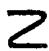
\includegraphics[keepaspectratio]{images/part001_579990b7.jpg}}

设 (C, d) 为一个复形。我们令 \(\mathbf{Z}(\mathbf{C}, d) = \operatorname{Ker}(d)\) , \(\mathbf{B}(\mathbf{C}, d) = \operatorname{Im}(d)\) ，它们是 C 的分次子模，分别称为 (C, d) 的闭链模和边缘模；\(\mathbf{Z}(\mathbf{C}, d)\) 和 \(\mathbf{B}(\mathbf{C}, d)\) 的齐次分量被记为 \(\mathbf{Z}_{n}(\mathbf{C}, d) = \mathbf{Z}^{-n}(\mathbf{C}, d)\) , \(\mathbf{B}_{n}(\mathbf{C}, d) = \mathbf{B}^{-n}(\mathbf{C}, d)\) ；我们有 \(\mathbf{Z}_{n}(\mathbf{C}, d) = \operatorname{Ker}(d_{n})\) , \(\mathbf{B}_{n}(\mathbf{C}, d) = \operatorname{Im}(d_{n+1})\) , \(\mathbf{Z}^{n}(\mathbf{C}, d) = \operatorname{Ker}(d^{n})\) , \(\mathbf{B}^{n}(\mathbf{C}, d) = \operatorname{Im}(d^{n-1})\) .

由于 \(d \circ d = 0\) ，我们有 \(\mathrm{B}(\mathrm{C}) \subset \mathrm{Z}(\mathrm{C})\) ；两个闭链若其差为一个边缘，则称它们是同调的；商分次模 \(\mathrm{H}(\mathrm{C}, d) = \mathrm{Z}(\mathrm{C}, d)/\mathrm{B}(\mathrm{C}, d)\) 被称为 \((\mathrm{C}, d)\) 的同调模；其元素是同调类；其齐次分量记为 \(\mathrm{H}_n(\mathrm{C}, d) = \mathrm{H}^{-n}(\mathrm{C}, d)\) 。

例。--- 若 C 的微分为零，则有 \(Z(C) = C\) , \(B(C) = 0\) ，且 \(H(C)\) 典范地等同于 \(C\) 。

我们有正合序列，称为典范的：

\((I_{n})\)

\[
0 \longrightarrow \mathrm{Z} _ {n} (\mathrm{C}) \longrightarrow \mathrm{C} _ {n} \stackrel {\delta_ {n}} {\longrightarrow} \mathrm{B} _ {n - 1} (\mathrm{C}) \longrightarrow 0\tag{\((\mathrm{II}_{n})\)}
\]

\[
0 \longrightarrow \mathrm{B} _ {n} (\mathrm{C}) \longrightarrow \mathrm{Z} _ {n} (\mathrm{C}) \longrightarrow \mathrm{H} _ {n} (\mathrm{C}) \longrightarrow 0
\]

\((\mathrm{III}_{n})\)

\[
0 \longrightarrow \mathrm{B} _ {n} (\mathrm{C}) \longrightarrow \mathrm{C} _ {n} \longrightarrow \mathrm{C} _ {n} / \mathrm{B} _ {n} (\mathrm{C}) \longrightarrow 0
\]

\((\mathrm{IV}_n)\)

\[
0 \longrightarrow \mathrm{H} _ {n} (\mathrm{C}) \longrightarrow \mathrm{C} _ {n} / \mathrm{B} _ {n} (\mathrm{C}) \stackrel {\overline {{\delta}} _ {n}} {\longrightarrow} \mathrm{B} _ {n - 1} (\mathrm{C}) \longrightarrow 0
\]

其中 \(\delta_{n}\) 和 \(\overline{\delta}_{n}\) 由 \(d_{n}\) 推出。通过结合 \((\mathrm{IV}_{n})\) 和 \((\mathrm{II}_{n-1})\) ，得到正合序列

\[
0 \rightarrow \mathrm{H} _ {n} (\mathrm{C}) \rightarrow \mathrm{C} _ {n} / \mathrm{B} _ {n} (\mathrm{C}) \rightarrow \mathrm{Z} _ {n - 1} (\mathrm{C}) \rightarrow \mathrm{H} _ {n - 1} (\mathrm{C}) \rightarrow 0,\tag{\((\mathbf{V}_n)\)}
\]

将 n 换成 -n，也可将它写成

\[
0 \rightarrow \mathrm{H} ^ {n} (\mathrm{C}) \rightarrow \mathrm{C} ^ {n} / \mathrm{B} ^ {n} (\mathrm{C}) \rightarrow \mathrm{Z} ^ {n + 1} (\mathrm{C}) \rightarrow , \mathrm{H} ^ {n + 1} (\mathrm{C}) \rightarrow 0.\tag{\((\mathbf{V}^n)\)}
\]

定义2.——设(C, d)和(C', d')是两个复形。从 (C, d) 到 (C', d') 的态射 \(^{1}\) 是从 C 到 C' 的次数为 0 的分次 A-同态 u，使得

\[
d ^ {\prime} \circ u = u \circ d.
\]

对于每一个 \(n\) ，我们有 \(d_n' \circ u_n = u_{n-1} \circ d_n\) 和 \(d''n \circ u^n = u^{n+1} \circ d^n\) 。我们有

\[
u (\mathbf {Z} (\mathbf {C})) \subset \mathbf {Z} (\mathbf {C} ^ {\prime}), \quad u (\mathbf {B} (\mathbf {C})) \subset \mathbf {B} (\mathbf {C} ^ {\prime}),
\]

并且我们用 \(Z(u):Z(C)\to Z(C')\) , \(B(u):B(C)\to B(C')\) , \(H(u):H(C)\to H(C')\) 表示由它们推出的A-模同态；这些态射的齐次分量记为 \(Z_{n}(u)\) , \(Z^{n}(u)\) , \ldots{}

若 \(v\) 是另一个从 \((\mathbf{C}, d)\) 到 \((\mathbf{C}', d')\) 的态射，则 \(u + v\) 是从 \((\mathbf{C}, d)\) 到 \((\mathbf{C}', d')\) 的态射，并且我们有

\[
\mathbf {Z} (u + v) = \mathbf {Z} (u) + \mathbf {Z} (v), \quad \mathbf {B} (u + v) = \mathbf {B} (u) + \mathbf {B} (v), \quad \mathbf {H} (u + v) = \mathbf {H} (u) + \mathbf {H} (v)
\]

类似地，若A是交换环 \(k\) 上的代数，且如果 \(\lambda \in k\) ，则 \(\lambda u\) 是从 \((C, d)\) 到 \((C', d')\) 的态射，并且我们有

\[
\mathbf {Z} (\lambda u) = \lambda \mathbf {Z} (u), \quad \mathbf {B} (\lambda u) = \lambda \mathbf {B} (u), \quad \mathbf {H} (\lambda u) = \lambda \mathbf {H} (u).
\]

若 \(u': (C', d') \to (C'', d'')\) 是另一个复形态射，则 \(u' \circ u\) 是从 \((C, d)\) 到 \((C'', d'')\) 的态射，并且我们有

\[
\mathrm{Z} \left(u ^ {\prime} \circ u\right) = \mathrm{Z} \left(u ^ {\prime}\right) \circ \mathrm{Z} (u), \quad \mathrm{B} \left(u ^ {\prime} \circ u\right) = \mathrm{B} \left(u ^ {\prime}\right) \circ \mathrm{B} (u), \quad \mathrm{H} \left(u ^ {\prime} \circ u\right) = \mathrm{H} \left(u ^ {\prime}\right) \circ \mathrm{H} (u).
\]

显然，双射态射即同构。

定义3.——设(C, d)和(C', d')是两个复形。从(C, d)到(C', d')的同调态射（或拟同构）是一个从(C, d)到(C', d')的态射u，使得H(u)是双射。

每个同构都是同调态射，并且由同调态射复合而成的任何态射都是同调态射。

称(C, d)具有零同调，若H(C) = 0，即若唯一的复形态射 \(0 \rightarrow C\) （相应地，C → 0）是一个同调态射。称（C, d）在降次数 n（相应地，在升次数 n）上是零调的，如果 \(\mathrm{H}_{n}(\mathrm{C}) = 0\) (相应地， \(\mathrm{H}^{n}(\mathrm{C}) = 0\) ).

设 (C, d) 为一个复形且 \(p \in Z\) ；(C, d) 的第 p 次平移是如下得到的复形 (C(p), d(p))：C(p) 是通过将 C 的分次平移 p 得到的 A-模（II，第 163 页；例 3），因此

\[
\mathrm{C} (p) _ {n} = \mathrm{C} _ {n + p}, \quad \mathrm{C} (p) ^ {n} = \mathrm{C} ^ {n - p};
\]

特别地 \(\mathbf{C}(p)_{0} = \mathbf{C}_{p}\) ；还需注意 C 是其分次子模 \(\mathbf{C}_{p}(-p)\) , \(p \in \mathbf{Z}\) （相应地， \(\mathbf{C}^{p}(p)\) , \(p \in \mathbf{Z}\) ）的直和。定义 \(d(p) = (-1)^{p} d\) 。我们有 \(\mathbf{Z}(\mathbf{C}(p)) = \mathbf{Z}(\mathbf{C})(p)\) , \(\mathbf{B}(\mathbf{C}(p)) = \mathbf{B}(\mathbf{C})(p)\) 和 \(\mathrm{H}(\mathbf{C}(p)) = \mathrm{H}(\mathbf{C})(p)\) 。

例如， \(d\) 是从 C 到 C(-1) 的复形态射，并且

\[
\mathrm{H} (d): \mathrm{H} (\mathbf {C}) \to \mathrm{H} (\mathbf {C}) (- 1)
\]

是零。

对于每个复形态射 \(u:(\mathbf{C},d)\to(\mathbf{C}^{\prime},d^{\prime})\) ，以及每个 \(p\in\mathbf{Z}\) , \(u\) 也是从 \((\mathbf{C}(p),d(p))\) 到 \((\mathbf{C}^{\prime}(p),d^{\prime}(p))\) 的态射；它有时被记为 \(u(p)\) 并且我们有

\[
u (p) _ {n} = u _ {n + p}, \quad u (p) ^ {n} = u ^ {n - p}.
\]
% semantic-fragments: legacy-input-seam
\relax{}
\subsection{复形的运算}

在集合 A × A 上，这两个运算

\[
\begin{array}{l} (a, b) + (a ^ {\prime}, b ^ {\prime}) = (a + a ^ {\prime}, b + b ^ {\prime}) \\ (a, b) (a ^ {\prime}, b ^ {\prime}) = (a a ^ {\prime}, a b ^ {\prime} + b a ^ {\prime}) \end{array}
\]

定义一个环结构，记为 A(ε)，其单位元为 1 = (1, 0)；嵌入映射 a ↦ (a, 0) = a1 使得 A 可被等同于 A(ε) 的一个子环；模 A(ε) 是自由的，其基为 \{ 1, ε \} 其中 ε = (0, 1)；我们有 ε² = 0，且 ε 在 A(ε) 中是中心的。

当A是交换的时， \(\mathrm{A}(\varepsilon)\) 是 A 上的双数代数（III，第 15 页）。赋予 \(\mathrm{A}(\varepsilon)\) 环分次结构（II，第164页），其中 \(\mathrm{A}(\varepsilon)_{0} = \mathrm{A}.1\) , \(\mathrm{A}(\varepsilon)_{-1} = \mathrm{A}. \varepsilon\) ，且 \(\mathrm{A}(\varepsilon)_{n} = 0\) （当 \(n \neq 0, -1\) ）。显然，在一个集合 C 上给出 A-复形结构，等同于在 C 上给出一个 \(\mathrm{A}(\varepsilon)\) 分次模结构，其中微分 d 对应于位似 \(\varepsilon_{C}\) ；同样地，复形的态射对应于 \(\mathrm{A}(\varepsilon)\) 分次模的次数为 0 的分次同态。因此， \(\mathrm{A}(\varepsilon)\) 分次模与 A-复形的结构种类是等价的（E, IV, 第 9-10 页）。我们将利用这一事实，将分次模理论中的通常概念移植到复形理论中。

对于分次子 A(ε)-模的概念，对应的是子复形的概念：因此，复形 (C, d) 的子复形是 C 的一个分次子模 C'，使得对每个 \(n \in Z\) , \(d_{n}(C_{n}') \subset C_{n-1}'\) ；若用 \(d'\) 表示由 d 诱导的从 C' 到 C' 的分次 A-同态，则 (C', d') 是一个复形结构，称为由 (C, d) 诱导的结构。除非另有明确说明，每个子复形都配备诱导结构。

我们将其留给读者，按照下面的词典，类似地详细阐述复形的商复形、复形的正合列、复形态射的核、余核和像的概念：

分次商 A(ε)-模

= 商复形，

次数为 0 的分次 A(ε)-同态的核、余核、像 \} 复形态射的核、余核、像，

分次A(ε)-模的正合列以及次数为0的分次同态 \} = 复形的正合列。

例如，第 1 号中的典范正合列给出复形的正合列，称为典范的。

\begin{enumerate}
\def\labelenumi{(\Roman{enumi})}
\tightlist
\item
\end{enumerate}

\[
0 \longrightarrow \mathrm{Z} (\mathrm{C}) \longrightarrow \mathrm{C} \stackrel {\delta} {\longrightarrow} \mathrm{B} (\mathrm{C}) (- 1) \longrightarrow 0,\tag{II}
\]

\[
0 \longrightarrow \mathrm{B} (\mathrm{C}) \longrightarrow \mathrm{Z} (\mathrm{C}) \longrightarrow \mathrm{H} (\mathrm{C}) \longrightarrow 0,\tag{III}
\]

\[
0 \longrightarrow \mathrm{B} (\mathrm{C}) \longrightarrow \mathrm{C} \longrightarrow \mathrm{C} / \mathrm{B} (\mathrm{C}) \longrightarrow 0,\tag{IV}
\]

\[
0 \longrightarrow \mathrm{H} (\dot {\mathrm{C}}) \longrightarrow \mathrm{C} / \mathrm{B} (\mathrm{C}) \stackrel {\delta} {\longrightarrow} \mathrm{B} (\mathrm{C}) (- 1) \stackrel {\cdot} {\longrightarrow} 0,\tag{V}
\]

\[
0 \longrightarrow \mathrm{H} (\mathrm{C}) \longrightarrow \mathrm{C} / \mathrm{B} (\mathrm{C}) \longrightarrow \mathrm{Z} (\mathrm{C}) (- 1) \longrightarrow \mathrm{H} (\mathrm{C}) (- 1) \longrightarrow 0.
\]

类似地，可以定义复形的直和、复形的归纳系以及复形的归纳系的归纳极限等概念。

设 \((\mathbf{C}_{i}, d_{i})\) 为一族复形。称此族的积，并记作 \(\prod_{i \in I} (\mathbf{C}_{i}, d_{i})\)，是按如下方式得到的复形 \((\mathbf{C}, d)\)：

\begin{enumerate}
\def\labelenumi{\alph{enumi})}
\item
  对于每个 \(n \in Z\) , \(C_{n}\) 是直积 A-模 \(\prod_{i \in I} (\mathbf{C}_{i})_{n}\)，即给定复形的齐次分量 \((\mathbf{C}_{i})_{n}\) 的直积
\item
  对于每个 \(n \in Z\) , \(d_{n} : C_{n} \to C_{n-1}\) 是A-同态，其分量为 \((d_{i})_{n}\) .
\end{enumerate}

当 I 有限时， \(\prod_{i\in I}(\mathbf{C}_{i},d_{i})\) 等于 \(\bigoplus_{i\in I}(\mathbf{C}_{i},d_{i})\) 。应当注意，一般而言，积复形 \(\prod_{i\in I}(\mathbf{C}_{i},d_{i})\) 的底层 A-模不是直积 A-模 \(\prod_{i\in I}\mathbf{C}_{i}\) .

考虑一个族（相应地，一个滤过归纳系） \((\mathbf{C}_i)_{i\in I}\) 。设 C 为 \(C_i\) 的直和（相应地，归纳极限），并设 \(\alpha_{i}:C_{i}\to C\) 为典范同态。则 \(\mathrm{H}(\alpha_{i}): \mathrm{H}(\mathrm{C}_{i})\to \mathrm{H}(\mathrm{C})\) 定义了从 \(\bigoplus_{i\in I}\mathrm{H}(\mathrm{C}_{i})\) （相应地， \(\varinjlim_{i\in I}\mathrm{H}(\mathrm{C}_{i})\) ）到 \(\mathrm{H}(\mathrm{C})\) 中的一个次数为 0 的、称为典范的分次同态。同样地，典范投影 \(\prod_{i\in I}\mathrm{C}_{i}\to \mathrm{C}_{i}\) 定义了从 \(\mathrm{H}(\prod \mathrm{C}_i)\) 到 \(\prod (\mathrm{H}(\mathrm{C}_i))\) 的一个次数为 0 的、称为典范的分次同态 .

命题1. --- 对于每个复形族 \((\mathbf{C}_{i})_{i\in I}\) ，典范同态

\[
\bigoplus_ {i \in \mathbf {I}} \mathrm{H} (\mathrm{C} _ {i}) \rightarrow \mathrm{H} \left(\bigoplus_ {i \in \mathbf {I}} \mathrm{C} _ {i}\right), \quad \mathrm{H} \left(\prod_ {i \in \mathbf {I}} \mathrm{C} _ {i}\right)\rightarrow \prod_ {i \in \mathbf {I}} \mathrm{H} (\mathrm{C} _ {i})\tag{2}
\]

都是双射的。

对于复形的每个滤过归纳系 \((\mathbf{C}_{i})_{i\in\mathbf{I}}\) ，典范同态

\[
\varinjlim_ {i \in \mathrm{I}} \mathrm{H} (\mathrm{C} _ {i}) \to \mathrm{H} (\varinjlim_ {i \in \mathrm{I}} \mathrm{C} _ {i})\tag{3}
\]

是双射。

这直接由II，第14页，命题7的推论1，第11页，命题5的推论，以及第91页，命题3得出。

\subsection{连接同态与同调正合列}

在本节中，我们考虑复形的一个正合列

\[
0 \longrightarrow \mathrm{C} ^ {\prime} \stackrel {u} {\longrightarrow} \mathrm{C} \stackrel {v} {\longrightarrow} \mathrm{C} ^ {\prime \prime} \longrightarrow 0;
\]

用同一字母d表示C、C'和C''的微分\,'.

设 \(\Gamma\) 为由 \(x \in \mathbf{C}\) 中满足 \(dx \in \operatorname{Im}(u)\) 的元素组成的集合；对于 \(x \in \Gamma\) ，我们有

\[
d \left(^ {- 1} u ^ {1} (d x)\right) = ^ {- 1} u ^ {1} (d d (x)) = 0,
\]

因此 \(\overline{u}^{1}(dx)\in\mathbf{Z}(\mathbf{C}^{\prime})\) ；我们还有 \(dv(x)=v(dx)\in\operatorname{Im}(v\circ u)=0\) ，因此 \(v(x)\in\mathbf{Z}(\mathbf{C}^{\prime\prime})\) ；于是考虑线性映射 \(\varphi:\Gamma\to\mathrm{H}(\mathbf{C}^{\prime\prime})\times\mathrm{H}(\mathbf{C}^{\prime})\) ，它将每个元素 \(x\in\Gamma\) 映到 \((v(x),\overline{u}^{1}(dx))\) 的类 .

引理1. —— \(\varphi(\Gamma)\) （ \(\Gamma\) 在 \(\mathrm{H}(\mathbf{C}^{\prime\prime}) \times \mathrm{H}(\mathbf{C}^{\prime})\) 中的像）是从 \(\mathrm{H}(\mathbf{C}^{\prime\prime})\) 到 \(\mathrm{H}(\mathbf{C}^{\prime})\) 的一个次数为 -1 的分次 A-同态的图 .

\begin{enumerate}
\def\labelenumi{\alph{enumi})}
\item
  若 \(x \in \Gamma\) 且 \(v(x) \in \mathbf{B}(\mathbf{C}'')\) ，则 \(\bar{u}^1(dx) \in \mathbf{B}(\mathbf{C}')\) ：确实存在 \(z'' \in \mathbf{C}''\) 使得 \(v(x) = dz''\) ，则 \(z \in \mathbf{C}\) 使得 \(z'' = v(z)\) ，因此 \(v(x) = v(dz)\) ，则 \(t' \in \mathbf{C}'\) 使得 \(x - dz = u(t')\) ，它给出 \(dx = u(dt')\) ，因此 \(\bar{u}^1(dx) = dt' \in \mathbf{B}(\mathbf{C}')\) .
\item
  \(\mathbf{Z}(\mathbf{C}^{\prime \prime})\) 中的每个元素都是 \(v\) 作用于某个元素 \(x\) （属于 \(\mathbf{C}\) 且满足 \(v(dx) = 0\) ，即\(dx \in \operatorname{Im} u\) ，亦即 \(x \in \Gamma\) ）的像 .
\item
  由a)和b)可知 \(\varphi(\Gamma)\) 确实是一个函数图；由于 \(\varphi\) 是双齐次的，且双次数为 \((0, -1)\) ，这完成了证明。
\end{enumerate}

由此定义的从 H(C'') 到 H(C') 的次数为 -1 的分次 A-同态称为相对于正合列 (u, v) 的连接同态；它记为 \(\partial(u, v)\) 或 \(\partial_{u,v}\) 或简记为 \(\partial\) 。其齐次分量记为

\[
\partial_ {n} (u, v): \mathrm{H} _ {n} (\mathbf {C} ^ {\prime \prime}) \rightarrow \mathrm{H} _ {n - 1} (\mathbf {C} ^ {\prime}) \quad \text { and } \quad \partial^ {n} (u, v): \mathrm{H} ^ {n} (\mathbf {C} ^ {\prime \prime}) \rightarrow \mathrm{H} ^ {n + 1} (\mathbf {C} ^ {\prime}).
\]

根据定义，为了构造类 \(\alpha\in\mathrm{H}_{n}(\mathbf{C}^{\prime\prime})\) 在 \(\partial\) 下的像，我们选取一个闭链 \(z^{\prime\prime}\in\mathbf{Z}_{n}(\mathbf{C}^{\prime\prime})\) （它代表类 \(\alpha\) ），然后选取一个元素 \(x\) （属于 \(\mathbf{C}_{n}\) ），使得 \(v(x)=z^{\prime\prime}\) ；于是 \(dx\) 具有 \(u(t')\) 的形式， \(t^{\prime}\in\mathbf{C}_{n-1}^{\prime}\) ，而 \(\partial(\alpha)\) 是 \(t'\) 的同调类 .

用对应的话来说， \(\partial_{n}(u,v)\) 因此是由对应 \(u_{n-1}^{-1}\circ d_{n}\circ v_{n}^{-1}\) （介于 \(\mathbf{C}_{n}^{\prime\prime}\) 与 \(\mathbf{C}_{n-1}^{\prime}\) 之间）通过先过渡到子集 \(\mathbf{Z}_{n}(\mathbf{C}^{\prime\prime})\) 与 \(\mathbf{Z}_{n-1}(\mathbf{C}^{\prime})\) 、再过渡到它们的商 \(\mathbf{H}_{n}(\mathbf{C}^{\prime\prime})\) 与 \(\mathbf{H}_{n-1}(\mathbf{C}^{\prime})\) 而得到的。这特别表明，如果把 \(\mathbf{C},\mathbf{C}^{\prime},\mathbf{C}^{\prime\prime},u,v\) 替换为 \(\mathbf{C}(p),\mathbf{C}^{\prime}(p),\mathbf{C}^{\prime\prime}(p),u(p),v(p)\) ，则有

\[
\partial (u (p), v (p)) = (- 1) ^ {p} \partial (u, v);\tag{4}
\]

同样地，如果 \(\lambda\) 与 \(\mu\) 是 A 的中心的两个可逆元素，则有

\[
\partial (\lambda u, \mu v) = \lambda^ {- 1} \mu^ {- 1} \partial (u, v).\tag{5}
\]

还可以将 \(\partial(u,v)\) 与蛇形图（X，第 4 页）联系起来。根据 loc. cit.，命题 2，序列

\[
0 \longrightarrow Z _ {n} (C ^ {\prime}) \xrightarrow {Z _ {n} (u)} Z _ {n} (C) \xrightarrow {Z _ {n} (v)} Z _ {n} (C ^ {\prime \prime})
\]

以及

\[
\mathrm{C} _ {n} ^ {\prime} / \mathrm{B} _ {n} (\mathrm{C} ^ {\prime}) \xrightarrow {\overline {{{u}}} _ {n}} \mathrm{C} _ {n} / \mathrm{B} _ {n} (\mathrm{C}) \xrightarrow {\overline {{{v}}} _ {n}} \mathrm{C} _ {n} ^ {\prime \prime} / \mathrm{B} _ {n} (\mathrm{C} ^ {\prime}) \longrightarrow 0,
\]

其中 \(\overline{u}_{n}\) 与 \(\overline{v}_{n}\) 分别由 \(u\) 与 \(v\) 诱导，都是正合的。利用典范正合列 \((\mathrm{V}_{n})\) ，可以得到一个具有正合行和正合列的交换图

\[
\begin{array}{c c c c} 0 & 0 & 0 \\ \downarrow & \mathrm{H} _ {n} (\mathrm{C} ^ {\prime}) & \xrightarrow {\mathrm{H} _ {n} (u)} & \mathrm{H} _ {n} (\mathrm{C}) \\ \downarrow & \mathrm{C} _ {n} ^ {\prime} / \mathrm{B} _ {n} (\mathrm{C} ^ {\prime}) & \xrightarrow {\bar {u} _ {n}} & \mathrm{C} _ {n} / \mathrm{B} _ {n} (\mathrm{C}) \\ \downarrow & 0 \longrightarrow Z _ {n - 1} (\mathrm{C} ^ {\prime}) & \xrightarrow {Z _ {n - 1} (u)} & Z _ {n - 1} (\mathrm{C}) \\ \downarrow & H _ {n - 1} (\mathrm{C} ^ {\prime}) & \xrightarrow {\mathrm{H} _ {n - 1} (u)} & H _ {n - 1} (\mathrm{C}) \\ \downarrow & 0 & 0 & 0 \end{array}
\]

与这个图相关联的同态 \(\mathrm{H}_{n}(\mathbf{C}^{\prime \prime})\to \mathrm{H}_{n - 1}(\mathbf{C}^{\prime})\) （loc. cit.，命题 2，(iii)）按构造与 \(\partial_n(u,v)\) 一致。这也意味着同态序列 \((\mathrm{H}_n(u),\mathrm{H}_n(v),\partial_n(u,v),\mathrm{H}_{n - 1}(u),\mathrm{H}_{n - 1}(v))\) 是正合的；因此：

定理1. --- A-模同态的无穷序列

\[
\begin{array}{r l} \dots & \to \mathrm{H} _ {n + 1} (\mathrm{C} ^ {\prime \prime}) \xrightarrow {\partial_ {n + 1} (u , v)} \mathrm{H} _ {n} (\mathrm{C} ^ {\prime}) \xrightarrow {\mathrm{H} _ {n} (u)} \mathrm{H} _ {n} (\mathrm{C}) \xrightarrow {\mathrm{H} _ {n} (v)} \mathrm{H} _ {n} (\mathrm{C} ^ {\prime \prime}) \\ & \xrightarrow {\partial_ {n} (u , v)} \mathrm{H} _ {n - 1} (\mathrm{C} ^ {\prime}) \xrightarrow {\mathrm{H} _ {n - 1} (u)} \mathrm{H} _ {n - 1} (\mathrm{C}) \xrightarrow {\mathrm{H} _ {n - 1} (v)} \mathrm{H} _ {n - 1} (\mathrm{C} ^ {\prime \prime}) \xrightarrow {\partial_ {n - 1} (u , v)} \mathrm{H} _ {n - 2} (\mathrm{C} ^ {\prime}) \to \dots \end{array}
\]

是正合的。

这个序列称为与正合列 \((u, v)\) 相关联的同调正合列；它有时写成 A-模的正合三角形的形式

\[
\begin{array}{c} \mathrm{H(C)} \\ \mathrm{H(u)} \nearrow \searrow \mathrm{H(v)} \\ \mathrm {H(C^ {\prime})} \xleftarrow [ \partial (u , v) ]{} \mathrm {H(C^{\prime\prime})}. \end{array}
\]

推论1. --- 若复形 C、C'、C'' 中有两个具有零同调，则第三个也具有零同调。要使 u（相应地 v）为拟同构，必要且充分条件是 C''（相应地 C'）具有零同调。要使 \(\partial(u, v)\) 是双射的，必要且充分条件是 C 具有零同调。

推论2. —— 设u是一个复形态射。如果Ker u和Coker u具有零同调，则u是一个拟同构。

事实上，设 \(u: \mathrm{E} \to \mathrm{E}'\) 是一个复形态射。如果 Ker \(u\) （相应地 Coker \(u\) ）具有零同调，则典范态射 \(\mathrm{E} \to \operatorname{Im} u\) （相应地， \(\operatorname{Im} u \to \mathrm{E}'\) ）由推论 1 是一个拟同构。

命题 2. — 考虑一个具有正合行的复形交换图

\[
\begin{array}{c} 0 \longrightarrow \mathrm{C} ^ {\prime} \stackrel {{u}} {{\longrightarrow}} \mathrm{C} \stackrel {{v}} {{\longrightarrow}} \mathrm{C} ^ {\prime \prime} \longrightarrow 0 \\ f ^ {\prime} \Big \downarrow \qquad \qquad \qquad f \Big \downarrow \qquad \qquad f ^ {\prime \prime} \Big \downarrow \\ 0 \longrightarrow \mathrm{C} _ {1} ^ {\prime} \stackrel {{u _ {1}}} {{\longrightarrow}} \mathrm{C} _ {1} \stackrel {{v _ {1}}} {{\longrightarrow}} \mathrm{C} _ {1} ^ {\prime \prime} \longrightarrow 0. \end{array}
\]

则 \(\mathbf{H}(f')\circ \partial (u,v) = \partial (u_1,v_1)\circ \mathbf{H}(f'')\)

设 \(\alpha'' \in \mathrm{H}(\mathbf{C}'')\) ；令 \(z''\) 为类 \(\alpha''\) 的一个闭链，并令 \(x\) 为 C 的一个元素，使得 \(v(x) = z''\) ；我们有

\[
\begin{array}{r l} \big (\partial_ {u _ {1}, v _ {1}} \circ \mathrm{H} (f ^ {\prime \prime}) \big) (\alpha^ {\prime \prime}) = & \partial_ {u _ {1}, v _ {1}} (\overline {{f ^ {\prime \prime} (z ^ {\prime \prime})}}) = \overline {{u _ {1} ^ {- 1} (d f (x))}} = \overline {{f ^ {\prime} (u ^ {- 1} (d x))}} = \\ & = \mathrm{H} (f ^ {\prime}) (\overline {{u ^ {- 1} (d x)}}) = (\mathrm{H} (f ^ {\prime}) \circ \partial_ {u, v}) (\alpha^ {\prime \prime}). \end{array}
\]

例。— 设 C 是一个复形。考虑典范正合列

\[
0 \longrightarrow \mathrm{Z} (\mathrm{C}) \stackrel {j} {\longrightarrow} \mathrm{C} \stackrel {\delta} {\longrightarrow} \mathrm{B} (\mathrm{C}) (- 1) \longrightarrow 0,\tag{I}
\]

并设 \(i: \mathbf{B}(\mathbf{C}) \to \mathbf{Z}(\mathbf{C})\) 为典范嵌入。则连接同态 \(\partial(j, \delta): \mathrm{H}(\mathrm{B}(\mathrm{C})) (-1) \to \mathrm{H}(\mathrm{Z}(\mathrm{C})) (-1)\) 与 \(\mathrm{H}(i) (-1)\) 等同，这一点可以立即验证。由于 \(\mathrm{H}(\delta) = 0\) ，与（I）相关联的同调正合列分解为短正合列

\[
0 \longrightarrow \mathrm{B} _ {n} (\mathrm{C}) \stackrel {i} {\longrightarrow} Z _ {n} (\mathrm{C}) \stackrel {\mathrm{H} (j)} {\longrightarrow} \mathrm{H} _ {n} (\mathrm{C}) \longrightarrow 0.\tag{\((\mathrm{II}_{\mathfrak{n}})\)}
\]

* 应用：

\begin{enumerate}
\def\labelenumi{\arabic{enumi})}
\tightlist
\item
  奇异同调
\end{enumerate}

设 A 为一个环。对于每个拓扑空间 X，定义 X 的以 A 为系数的奇异复形 C(X, A) 如下：

在 \(\mathbf{R}^{(N)}\) 中，设 \((e_n)\) 为典范基；标准 \(n\) -单形定义为凸包 \(\Delta_n\) （即 \(\{e_0, \ldots, e_n\}\) 的凸包）。对于 \(i \in \{0, \ldots, n\}\) ，定义仿射映射 \(\iota_i: \Delta_{n-1} \to \Delta_n\) 如下： \(\iota_i(e_k) = e_k\) （当 \(k < i\) ）， \(\iota_i(e_k) = e_{k+1}\) （当 \(k \geqslant i\) ）。用 \(\mathbf{C}_n(\mathbf{X}, \mathbf{A})\) 表示 A-模 \(\mathbf{A}^{(\Sigma_n(\mathbf{X}))}\) ，其中 \(\Sigma_n(\mathbf{X})\) 是从 \(\Delta_n\) 到 \(\mathbf{X}\) 的连续映射的集合；当 \(n < 0\) 时，设 \(\mathbf{C}_n = 0\) 。对于 \(i \in \{0, \ldots, n\}\) ，定义线性映射 \(\partial_{n,i}: \mathbf{C}_n(\mathbf{X}, \mathbf{A}) \to \mathbf{C}_{n-1}(\mathbf{X}, \mathbf{A})\) 如下： \(\partial_{n,i}(e_s) = e_{s \circ \iota_i}\) （对 \(s \in \Sigma_n(\mathbf{X})\) ），并设 \(d_n = \Sigma (-1)^t \partial_{n,i}\) 。可以验证

\[
\dots \mathrm{C} _ {n} (\mathrm{X}, \mathrm{A}) \xrightarrow {d _ {n}} \mathrm{C} _ {n - 1} (\mathrm{X}, \mathrm{A}) \rightarrow \dots
\]

是一个复形。它的同调称为X以A为系数的奇异同调，记为H(X, A)或简记为H(X)。

若Y是X的子空间，则用C(X, Y, A)表示商复形C(X, A)/C(Y, A)，并用H(X, Y, A)表示其同调。由定理I可得如下正合列：

\[
\dots \rightarrow \mathrm{H} _ {n} (\mathrm{Y}, \mathrm{A}) \rightarrow \mathrm{H} _ {n} (\mathrm{X}, \mathrm{A}) \rightarrow \mathrm{H} _ {n} (\mathrm{X}, \mathrm{Y}, \mathrm{A}) \rightarrow \mathrm{H} _ {n - 1} (\mathrm{Y}, \mathrm{A}) \rightarrow \mathrm{H} _ {n - 1} (\mathrm{X}, \mathrm{A}) \rightarrow \dots
\]

\begin{enumerate}
\def\labelenumi{\arabic{enumi})}
\setcounter{enumi}{1}
\tightlist
\item
  有限胞腔复形
\end{enumerate}

设 X 是一个豪斯多夫拓扑空间。X 的一个有限胞腔分解由闭子空间的一个递增序列 \((X_{n})_{n\in\mathbb{Z}}\) 给出，满足以下条件：(i) \(X_{n} = \varnothing\) （当 n \textless{} 0 时）；

\begin{enumerate}
\def\labelenumi{(\roman{enumi})}
\setcounter{enumi}{1}
\item
  存在一个 N ，使得 \(X_{N} = X\) （因此 \(X_{n} = X\) ，只要 n \textgreater{} N）；
\item
  对所有 \(n\) ，空间 \(\mathbf{X}_{n} - \mathbf{X}_{n-1}\) 只有有限多个连通分支，称为维数为 \(n\) 的胞腔;
\item
  对于每一个n，以及对于每一个连通分支C（属于 \(X_{n} - X_{n-1}\) ），存在一个从维数为 n 的开欧几里得球 \(\dot{B}_{n}\) （TG, VI, 第 10 页）到 C 上的同胚映射，且该映射可延拓为从闭球到 X 中的连续映射。
\end{enumerate}

可以证明这些条件蕴含： \(\mathbf{H}_n(\mathbf{X}_n, \mathbf{X}_{n-1}, \mathbf{A})\) 是一个自由 A-模 \(\Gamma_n\) ，其秩等于维数为 \(n\) 的胞腔的个数，并且 \(\mathbf{H}_i(\mathbf{X}_n, \mathbf{X}_{n-1}, \mathbf{A}) = 0\) （当 \(i \neq n\) 时）。我们有 \(\mathbf{C}(\mathbf{X}_n, \mathbf{X}_{n-1}, \mathbf{A}) = \mathbf{C}(\mathbf{X}_n, \mathbf{X}_{n-2}, \mathbf{A}) / \mathbf{C}(\mathbf{X}_{n-1}, \mathbf{X}_{n-2}, \mathbf{A})\) ，由此得到一个正合列

\[
\mathrm{H} _ {n} \left(\mathrm{X} _ {n}, \mathrm{X} _ {n - 2}\right) \longrightarrow \mathrm{H} _ {n} \left(\mathrm{X} _ {n}, \mathrm{X} _ {n - 1}\right) \xrightarrow {d _ {n}} \mathrm{H} _ {n - 1} \left(\mathrm{X} _ {n - 1}, \mathrm{X} _ {n - 2}\right) \longrightarrow \mathrm{H} _ {n - 1} \left(\mathrm{X} _ {n}, \mathrm{X} _ {n - 2}\right),
\]

其中带有连接同态 \(d_{n}:\Gamma_{n}\to\Gamma_{n-1}\) 。我们有 \(d_{n}\circ d_{n+1}=0\) ，从而可以定义一个复形 \(\Gamma:\cdots\to\Gamma_{n}\xrightarrow{d_{n}}\Gamma_{n-1}\to\cdots\) .

正合列

\[
\mathrm{H} _ {n + 1} \left(\mathrm{X} _ {p}, \mathrm{X} _ {p - 1}\right)\rightarrow \mathrm{H} _ {n} \left(\mathrm{X} _ {p - 1}\right)\rightarrow \mathrm{H} _ {n} \left(\mathrm{X} _ {p}\right)\rightarrow \mathrm{H} _ {n} \left(\mathrm{X} _ {p}, \mathrm{X} _ {p - 1}\right)\rightarrow \mathrm{H} _ {n - 1} \left(\mathrm{X} _ {p - 1}\right)
\]

通过对 \(p\) 作归纳表明： \(\mathrm{H}_{n}(\mathrm{X}_{p})=0\) （当 \(p<n\) ）， \(\mathrm{H}_{n}(\mathrm{X}_{n})=\mathrm{Ker}\left(d_{n}:\Gamma_{n}\to\Gamma_{n-1}\right)\) ，并且 \(\mathrm{H}_{n}(\mathrm{X}_{p})=\mathrm{H}_{n}(\Gamma)\) （当 \(p>n\) ）。特别地， \(\mathrm{H}_{n}(\mathrm{X})\) 与 \(\mathrm{H}_{n}(\Gamma)\) 等同 .

示例。--- 考虑球面的乘积 \(\mathbf{S}_{2} \times \mathbf{S}_{2}\) 以及复射影空间 \(\mathbf{P}_{2}(\mathbf{C})\) 。设 \(b \in \mathbf{S}_{2}\) ；通过如下取定来定义胞腔分解 \((\mathrm{Y}_{n})\) （其中 \(\mathrm{Y} = \mathbf{S}_{2} \times \mathbf{S}_{2}\) ）：

\[
\mathrm{Y} _ {0} = \mathrm{Y} _ {1} = \{(b, b) \}, \quad \mathrm{Y} _ {2} = \mathrm{Y} _ {3} = (\{b \} \times \mathbf {S} _ {2}) \cup (\mathbf {S} _ {2} \times \{b \}) \quad \text {and} \quad \mathrm{Y} _ {4} = \mathbf {S} _ {2} \times \mathbf {S} _ {2};
\]

此分解有一个 0 维胞腔、两个 2 维胞腔和一个 4 维胞腔。相应复形的微分必然为零，因此 \(\mathrm{H}_{0}(\mathrm{Y})\) , \(\mathrm{H}_{2}(\mathrm{Y})\) 与 \(\mathrm{H}_{4}(\mathrm{Y})\) 分别是秩为 1、2 和 1 的自由模，并且 \(\mathrm{H}_{n}(\mathrm{Y}) = 0\) （当 \(n \notin \{0, 2, 4\}\) 时）.

我们得到一个胞腔分解 \((\mathbf{Z}_{n})\) ，即 \(\mathbf{P}_{2}(\mathbf{C})\) 的如下分解：

\[
\mathbf {Z} _ {0} = \mathbf {Z} _ {1} = \{c \}, \quad \mathbf {Z} _ {2} = \mathbf {Z} _ {3} = \mathbf {P} _ {1} (\mathbf {C}), \quad \mathbf {Z} _ {4} = \mathbf {P} _ {2} (\mathbf {C}),
\]

其中空间 \(\mathbf{P}_{1}(\mathbf{C})\) 嵌入在 \(\mathbf{P}_{2}(\mathbf{C})\) 中（TG，VIII，第20页），而 \(c\) 是 \(\mathbf{P}_{1}(\mathbf{C})\) 的一个点；这个分解有一个0维胞腔、一个2维胞腔和一个4维胞腔。这里复形的微分同样必然为零，因此可得 \(\mathbf{H}_{n}(\mathbf{P}_{2}(\mathbf{C}))\) 与 A 同构（当 \(n \in \{0, 2, 4\}\) ），否则为0。

由于所考虑的两个空间的 2 次同调模分别是秩为 2 和 1 的自由模，这两个空间不同胚。*

\subsection{同伦}

定义4.——设(C, d)和(C', d')为两个复形，并设f和g为从C到C'的两个态射。连接 f 到 g 的一个同伦是指从C到C'的任意次数为1的分次A-同态s，使得 \(g - f = d' \circ s + s \circ d\) .

我们称 f 与 g 同伦，如果存在一个连接 f 到 g 的同伦。

若 \(h\) 是从 \(C\) 到 \(C'\) 的第三个态射，且 \(s\) （相应地 \(t\) ）是连接 \(f\) 到 \(g\) （相应地 \(g\) 到 \(h\) ）的一个同伦，则 \(s + t\) 是连接 \(f\) 到 \(h\) 的一个同伦；因此，关系“f 与 g 是从 C 到 C' 的两个同伦的态射”是一个等价关系，其等价类称为从 C 到 C' 的态射的同伦类。

给定两个拓扑空间 X 和 Y，以及一个连续映射 \(f: \mathbf{X} \to \mathbf{Y}\) ，我们定义一个线性映射 \(f_{*}\) 从奇异复形（参见第 3 号）C(X, A) 到 C(Y, A)，即设定 \(f_{*}(e_{s}) = e_{f \circ s}\) （其中 \(s \in \Sigma_{n}(\mathbf{X})\) ）。这个映射是一个复形态射。

两个连续映射 \(f\) 与 \(g\) （从 X 到 Y）称为拓扑同伦的，如果存在一个连续映射 \(h\) ，它把 \([0, 1] \times X\) 映到 Y 中，使得 \(h(0, x) = f(x)\) 与 \(h(1, x) = g(x)\) （对所有 \(x \in X\) ）。我们证明，如果 \(f\) 与 \(g\) 是拓扑同伦的，则态射 \(f_*\) 与 \(g_*\) 在上述定义 4 的意义上是同伦的。正是这一事实构成了代数中所用术语的来源。*

命题3. --- 若f和g是从C到C'的两个同伦的态射，则H(f) = H(g)。

设 s 是从 f 到 g 的同伦。我们有

\[
(g - f) (\mathbf {Z} (\mathbf {C})) = (d ^ {\prime} \circ s + s \circ d) (\mathbf {Z} (\mathbf {C})) = (d ^ {\prime} \circ s) (\mathbf {Z} (\mathbf {C})) \subset \mathrm{B} (\mathbf {C} ^ {\prime}),
\]

因此 \(\mathrm{H}(g - f) = 0\) 且 \(\mathrm{H}(g) = \mathrm{H}(f)\) .

推论。--- 与拟同构同伦的态射是拟同构。

命题4. --- 设 C, C', D, D' 为四个复形， \(f: \mathbf{C} \to \mathbf{C}'\) , \(g: \mathbf{C} \to \mathbf{C}'\) , \(u: \mathbf{D} \to \mathbf{C}\) , \(v: \mathbf{C}' \to \mathbf{D}'\) 四个态射。若 s 是连接 \(f\) 到 \(g\) 的一个同伦，则 \(v \circ s \circ u\) 是连接 \(v \circ f \circ u\) 到 \(v \circ g \circ u\) 的一个同伦。如果 f 和 g 是同伦的，那么 \(v \circ f \circ u\) 与 \(v \circ g \circ u\) 也是同伦的 .

这是显然的。

推论。——设C、C′、C″为三个复形，f和g为从C到C′的两个态射， \(f_{1}\) 与 \(g_{1}\) 为从 C' 到 C'' 的两个态射。若 s 和 \(s_{1}\) 分别是连接 f 到 g 与连接 \(f_{1}\) 到 \(g_{1}\) 的同伦，则 \(s_{1} \circ f + g_{1} \circ s\) 是连接 \(f_{1} \circ f\) 到 \(g_{1} \circ g\) 的一个同伦。如果 f 与 \(f_{1}\) 分别同伦于 g 与 \(g_{1}\) ，则 \(f_{1} \circ f\) 同伦于 \(g_{1} \circ g\) .

事实上， \(s_{1} \circ f\) 连接 \(f_{1} \circ f\) 到 \(g_{1} \circ f\) ，而 \(g_{1} \circ s\) 连接 \(g_{1} \circ f\) 到 \(g_{1} \circ g\) .

定义 5. --- 复形的态射 \(f: \mathbb{C} \to \mathbb{C}'\) 称为同伦等价，如果存在一个态射 \(f': \mathbb{C}' \to \mathbb{C}\) 使得 \(f' \circ f\) 与 \(f \circ f'\) 分别同伦于 \(1_{\mathbb{C}}\) 与 \(1_{\mathbb{C}'}\) 。

显然， \(f'\) 因此也是一个同伦等价；人们也说 \(f'\) 是 \(f\) 在同伦意义下的逆。如果 \(f'\) 与 \(f_1'\) 都是 \(f\) 在同伦意义下的逆，则 \(f'\) 与 \(f_1'\) 是同伦的（事实上，由前述推论， \(f_1' = f_1' \circ 1_{\mathbf{C}'}\) 同伦于 \(f_1' \circ f \circ f'\) ，从而同伦于 \(1_{\mathbf{C}} \circ f' = f'\) ).

命题5. — 同伦等价是拟同构；由同伦等价复合而成的态射是同伦等价。与同伦等价同伦的态射是同伦等价。

设 \(f: \mathbf{C} \to \mathbf{C}'\) 与 \(f_1: \mathbf{C}' \to \mathbf{C}''\) 是复形的同伦等价， \(f': \mathbf{C}' \to \mathbf{C}\) 与 \(f_1': \mathbf{C}'' \to \mathbf{C}'\) 是同伦意义下互逆的态射。我们有

\[
\mathrm{H} (f ^ {\prime}) \circ \mathrm{H} (f) = \mathrm{H} (f ^ {\prime} \circ f) = \mathrm{H} (1 _ {\mathrm{C}}) = 1 _ {\mathrm{H(C)}} \quad (\text { prop. } 3)
\]

并且类似地 \(\mathrm{H}(f) \circ \mathrm{H}(f') = 1_{\mathrm{H}(\mathbb{C}')}\) ，因此 \(\mathrm{H}(f)\) 是双射且 \(f\) 是一个拟同构。另一方面， \((f' \circ f_1') \circ (f_1 \circ f)\) 同伦于 \(f' \circ 1_{\mathbb{C}'} \circ f\) （命题4），从而同伦于 \(1_{\mathbb{C}}\) ；同样地， \((f_1 \circ f) \circ (f' \circ f_1')\) 同伦于 \(1_{\mathbb{C}''}\) ，且 \(f_1 \circ f\) 是一个同伦等价。最后，如果 \(g: \mathbb{C} \to \mathbb{C}'\) 是同伦于 \(f\) 的一个态射，则 \(f' \circ g\) 同伦于 \(f' \circ f\) ，从而同伦于 \(1_{\mathbb{C}}\) ；同样地， \(g \circ f'\) 同伦于 \(f \circ f'\) ，从而同伦于 \(1_{\mathbb{C}'}\) ，且 \(g\) 是一个同伦等价。

推论。——设C、C'、D、D'为四个复形， \(f: \mathbf{C} \to \mathbf{C}'\) 一个态射， \(u: \mathbf{D} \to \mathbf{C}\) 与 \(v: \mathbf{C}' \to \mathbf{D}'\) 为同伦等价。要使 \(v \circ f \circ u\) 是同伦等价（相应地，拟同构），必要且充分的条件是 \(f\) 是一个。

若 \(f\) 是一个同伦等价（相应地，拟同构），则 \(v \circ f \circ u\) 由同伦等价（相应地，拟同构）复合而成，因此也是一个。反过来，设 \(\overline{u}\) 与 \(\overline{v}\) 是在同伦意义下逆于 \(u\) 与 \(v\) 的态射；则 \(\overline{v} \circ (v \circ f \circ u) \circ \overline{u}\) 由命题4同伦于 \(f\) ；因此由命题5及命题3的推论得出结论。

我们称复形C同伦于零，如果 \(1_{C}\) 同伦于零映射，即，若存在 C 的一个次数为 1 的分次 A-自同态 s，使得 \(1_{C} = s \circ d + d \circ s\) 。这也等价于说唯一态射 \(0 \to C\) (相应地， \(C \to 0\) )是一个同伦等价。一个同伦于零的复形具有零同调（命题5）。

例. --- 设 \(u: \mathbf{M} \to \mathbf{N}\) 与 \(v: \mathbf{N} \to \mathbf{P}\) 是 A-模的同态，使得 \(v \circ u = 0\) ；令 C 为满足下述条件的复形： \(\mathbf{C}_2 = \mathbf{M}\) , \(\mathbf{C}_1 = \mathbf{N}\) , \(\mathbf{C}_0 = \mathbf{P}\) , \(\mathbf{C}_i = 0\) 当 \(i \neq 0, 1, 2, d_2 = u, d_1 = v, d_i = 0\) 当 \(i \neq 1, 2\) 。则 C 的同调为零当且仅当序列 \(0 \to \mathbf{M} \xrightarrow{u} \mathbf{N} \xrightarrow{v} \mathbf{P} \to 0\) 是正合的。它同伦于零当且仅当该序列是分裂的。事实上，说 C 同伦于零意味着存在 A-同态 \(s: \mathbf{P} \to \mathbf{N}\) 与 \(t: \mathbf{N} \to \mathbf{M}\) 使得 \(v \circ s = 1_{\mathbf{P}}, s \circ v + u \circ t = 1_{\mathbf{N}}, t \circ u = 1_{\mathbf{M}}\) ；这蕴含该序列是分裂的；反之，若 \(s\) 是 \(v\) 的一个 A-线性截面，我们如下定义 \(t\) ： \(u \circ t = 1_{\mathbf{N}} - s \circ v\) ，这之所以可能，是因为 \(v \circ (1_{\mathbf{N}} - s \circ v) = v - v \circ s \circ v = 0\) .

\subsection{分裂复形}

命题6. — 设 (C, d) 是一个复形。以下条件等价：

\begin{enumerate}
\def\labelenumi{(\roman{enumi})}
\item
  存在从 (C, d) 到 (H(C), 0) 的同伦等价
\item
  存在一个次数为1的A-分次自同态s，使得 \(d = d \circ s \circ d\) ;
\item
  B(C) 与 Z(C) 是 C 的直和项；
\item
  (C, d) 是子复形的直和，这些子复形要么长度为 0，要么长度为 1 且同调为零。
\item
  \(\Rightarrow\) (ii)：设 \(\varphi: \mathbf{C} \to \mathbf{H}(\mathbf{C})\) 是一个同伦等价；则存在一个复形态射 \(\psi: \mathbf{H}(\mathbf{C}) \to \mathbf{C}\) 以及一个自同态 \(s\) （ \(\mathbf{C}\) 的、次数为 1 的），使得 \(\psi \circ \varphi = 1_{\mathbf{C}} - s \circ d - d \circ s\) 。我们有 \(d \circ \psi = \psi \circ 0 = 0\) ，因此
\end{enumerate}

\[
0 = d \circ \psi \circ \varphi = d - d \circ s \circ d - d \circ d \circ s = d - d \circ s \circ d, \quad \text {whence (ii)}.
\]

\begin{enumerate}
\def\labelenumi{(\roman{enumi})}
\setcounter{enumi}{1}
\item
  \(\Rightarrow\) (iii)：设 \(s\) 如(ii)中所述。则 \(d \circ (1_{\mathbb{C}} - s \circ d) = 0\) ，因此 \(1_{\mathbb{C}} - s \circ d\) 是 \(\mathbf{C}\) 到 \(\mathbf{Z}(\mathbf{C})\) 上的投影映射，且 \((d \circ s) \circ d = d\) ，因此 \(d \circ s\) 是 \(\mathbf{C}\) 到 \(\mathbf{B}(\mathbf{C})\) 上的投影映射 .
\item
  \(\Rightarrow\) (iv)：对每个 \(n\in\mathbf{Z}\) ，设 \(Z_{n}=Z_{n}(\mathrm{C})\) , \(B_{n}=B_{n}(\mathrm{C})\) ，并选取子模 \(K_{n}\) 与 \(B_{n}^{\prime}\) （含于 \(C_{n}\) ），使得 \(C_{n}=B_{n}^{\prime}\oplus Z_{n}\) , \(Z_{n}=K_{n}\oplus B_{n}\) 。然后
\end{enumerate}

\[
\mathrm{E} _ {(n)} = \mathrm{K} _ {n} (- n) \quad \text { and } \quad \mathrm{F} _ {(n)} = \mathrm{B} _ {n} ^ {\prime} (- n) \oplus \mathrm{B} _ {n - 1} (1 - n)
\]

是 (C, d) 的子复形；我们有 (C, d) = \(\bigoplus_{n \in \mathbf{Z}} (\mathrm{E}_{(n)} \oplus \mathrm{F}_{(n)})\) ；每个 \(\mathrm{E}_{(n)}\) 要么为零，要么长度为 0，每个 \(\mathrm{F}_{(n)}\) 要么为零，要么长度为 1 且同调为零，由此得 (iv)。

\begin{enumerate}
\def\labelenumi{(\roman{enumi})}
\setcounter{enumi}{3}
\tightlist
\item
  \(\Rightarrow\) (i)：只需注意当 C 的长度为零，或同调为零且长度为 1 时，(i) 成立。
\end{enumerate}

定义 6. --- 若复形 C 满足命题 6 的等价条件，则称其为分裂的。

满足命题 6 条件 (ii) 的 C 的自同态 s 称为 C 的一个分裂。

例子. --- 1) 具有零微分的复形是分裂的。

\begin{enumerate}
\def\labelenumi{\arabic{enumi})}
\setcounter{enumi}{1}
\item
  同伦于零的复形正是同调为零的分裂复形，即满足 H(C) = 0 且 Z(C) 是 C 的直和项的复形 C。
\item
  设 \(f: \mathbf{M} \to \mathbf{N}\) 是 A-模的同态，且 C 是满足 \(\mathbf{C}_1 = \mathbf{M}, \mathbf{C}_0 = \mathbf{N}, \mathbf{C}_i = 0\) 当 \(i \neq 0, 1, d_1 = f, d_i = 0\) 当 \(i \neq 1\) 的复形。则 C 是分裂的当且仅当 Ker \(f\) 是 M 的直和项且 Im \(f\) 是 N 的直和项。
\item
  只要 B(C) 与 H(C) 是投射的（或只要对每个 n， \(B_{n}(C)\) 与 \(H_{n}(C)\) 是内射的），复形 C 就是分裂的。事实上，由第 1 号的正合列 \((I_{n})\) 到 \((IV_{n})\) 可知，此时 Z(C) 是 C 的直和项且 B(C) 是 Z(C) 的直和项（相应地，B(C) 是 C 的直和项且 Z(C)/B(C) 是 C/B(C) 的直和项）。
\item
  特别地，若 A 是主理想环，则自由复形 C 是分裂的当且仅当 H(C) 是自由的（即对每个 n ∈ Z，H \(_{n}\) (C) 是自由的）。
\end{enumerate}

注. --- a) 假设分次 A-模的典范正合列

\[
0 \to \mathrm{B} (\mathrm{C}) \to \mathrm{Z} (\mathrm{C}) \xrightarrow {\pi} \mathrm{H} (\mathrm{C}) \to 0\tag{II}
\]

是分裂的（例如当 H(C) 是投射的，或对每个 n，B \(_{n}\) (C) 是内射的时成立）；设 σ : H(C) → Z(C) 是 π 的一个分次 A-线性截面，并设 ψ 为从 H(C) 到 C 的映射 x ↦ σ(x)。则 ψ 是从 (H(C), 0) 到 C 的一个拟同构，使得 H(ψ) = 1 \(_{H(C)}\) .

\begin{enumerate}
\def\labelenumi{\alph{enumi})}
\setcounter{enumi}{1}
\tightlist
\item
  假设分次 A-模的典范正合列
\end{enumerate}

\[
0 \rightarrow \mathrm{H} (\mathrm{C}) \stackrel {i} {\rightarrow} \mathrm{C} / \mathrm{B} (\mathrm{C}) \rightarrow \mathrm{B} (\mathrm{C}) (- 1) \rightarrow 0\tag{IV}
\]

是分裂的（例如当 B(C) 是投射的，或 H \(_{n}\) (C) 对每个 \(n\) 是内射的时成立）；设 \(\tau: \mathbf{C} / \mathbf{B}(\mathbf{C}) \to \mathbf{H}(\mathbf{C})\) 是 \(i\) 的一个分次 A-线性收缩，并设 \(\varphi\) 为从 C 到 \(\mathbf{H}(\mathbf{C})\) 的同态，它把 C 的每个元素映到该元素在 \(\tau\) 下的像，即该元素模 \(\mathbf{B}(\mathbf{C})\) 的类的像。则 \(\varphi\) 是从 C 到 \((\mathbf{H}(\mathbf{C}), 0)\) 的一个拟同构，使得 \(\mathbf{H}(\varphi) = 1_{\mathbf{H}(\mathbf{C})}\) .

\subsection{复形态射的锥与柱}

设 \(u:(\mathbf{C}^{\prime},d^{\prime})\to(\mathbf{C},d)\) 是复形的一个态射。设 \(\operatorname{Cyl}(u)\) 与 \(\operatorname{Con}(u)\) 为 \(\text{分次 A-模 }\operatorname{Cyl}(u)=\mathbf{C}^{\prime}\oplus\mathbf{C}^{\prime}(-1)\oplus\mathbf{C}\) , \(\operatorname{Con}(u)=\mathbf{C}^{\prime}(-1)\oplus\mathbf{C}\) ，并让我们定义次数为 \((-1)\) 的分次 A-线性映射

\(\overline{\mathbf{D}}:\operatorname {Cyl}(u)\to \operatorname {Cyl}(u),\quad \overline{\mathbf{D}} (x^{\prime},y^{\prime},x) = (d^{\prime}x^{\prime} + y^{\prime}, - d^{\prime}y^{\prime},dx - u(y^{\prime})),\)

D : Con \((u) \to \text{Con}(u)\) , D \((y', x) = (-d'y', dx - u(y'))\) .

（此处以及后文中，我们用 \(x\) , \(y\) , \ldots{} 表示 C 的任意元素，用 \(x'\) , \(y'\) , \ldots{} 表示 C' 的任意元素。）

引理2. --- (Cyl \((u)\) , \(\overline{\mathbf{D}}\) ) 和 (Con \((u)\) , D) 是A-模的复形。

确实，我们有

\[
\begin{array}{r l} \overline {{\mathbf {D}}} \circ \overline {{\mathbf {D}}} (x ^ {\prime}, y ^ {\prime}, x) & = \overline {{\mathbf {D}}} (d ^ {\prime} x ^ {\prime} + y ^ {\prime}, - d ^ {\prime} y ^ {\prime}, d x - u (y ^ {\prime})) = \\ & = (d ^ {\prime} (d ^ {\prime} x ^ {\prime} + y ^ {\prime}) - d ^ {\prime} y ^ {\prime}, - d ^ {\prime} (- d ^ {\prime} y ^ {\prime}), d (d x - u (y ^ {\prime})) - u (- d ^ {\prime} y ^ {\prime})) = 0 \end{array}
\]

因为 \(d' \circ d' = 0\) , \(d \circ d = 0\) 且 \(d \circ u = u \circ d'\) 。同样地 \(D \circ D = 0\) .

定义7.——复形Cyl(u)和Con(u)分别称为态射u的柱和锥。

例. --- 设 \(u: \mathbf{M} \to \mathbf{N}\) 是 A-模的同态；则 \(\operatorname{Cyl}(u)\) 与 \(\operatorname{Con}(u)\) 的仅有的非零齐次分量是

\[
\operatorname{Cyl} _ {1} (u) = \mathrm{M}, \quad \operatorname{Cyl} _ {0} (u) = \mathrm{M} \oplus \mathrm{N},
\]

\[
\operatorname{Con} _ {1} (u) = \mathrm{M}, \quad \operatorname{Con} _ {0} (u) = \mathrm{N},
\]

并且我们有 \(\overline{\mathrm{D}}(m) = (m, -u(m))\) , \(\mathrm{D}(m) = -u(m)\) （对 \(m \in \mathbf{M}\) ）；因此，

\[
\mathrm{H} _ {1} (\text { Con } (u)) = \operatorname{Ker} (u), \quad \mathrm{H} _ {0} (\text { Con } (u)) = \operatorname{Coker} (u).
\]

复形 \(\Gamma(s)\) （与空间 \(\{s\}\) 相关联，后者赋予其唯一的胞腔分解）约化为模 A，并被等同于 \(\Gamma(\text{Con}(f))\) 的一个子复形；用 \(\Gamma(\text{Con}(f), s)\) 表示商复形。映射 \(f\) 定义了复形的一个态射 \(\Gamma(f): \Gamma(X) \to \Gamma(Y)\) ，并且可以证明，复形 \(\Gamma(\text{Cyl}(f))\) 与 \(\Gamma(\text{Con}(f), s)\) 分别被等同于 \(\text{Cyl}(\Gamma(f))\) 与 \(\text{Con}(\Gamma(f))\) .

此外，在不对 X 和 Y 作任何假设的情况下，可将 \(f\) 与复形的一个态射 \(f_{*}: \mathrm{C}(\mathrm{X}, \mathrm{A}) \to \mathrm{C}(\mathrm{Y}, \mathrm{A})\) 相关联。可以构造从 \(\mathrm{Cyl}(f_{*})\) 到 \(\mathrm{C}(\mathrm{Cyl}(f), \mathrm{A})\) 以及从 \(\mathrm{Con}(f_{*})\) 到 \(\mathrm{C}(\mathrm{Con}(f), \{s\}, \mathrm{A})\) 的单射同伦等价。

设 \(\tilde{f}: X \to \text{Cyl}(f)\) 是把 \(x\) 映到 \((0, x)\) 的像的映射， \(\alpha: Y \to \text{Cyl}(f)\) 为典范映射， \(\beta: \text{Cyl}(f) \to Y\) 为这样的映射：它把 \(y\) 映到其在 \(\text{Cyl}(f)\) 中的像（当 \(y \in Y\) ），并把 \(f(x)\) 映到 \((t, x)\) 在 \(\text{Cyl}(f)\) 中的像（当 \(t \in [0, 1]\) 且 \(x \in X\) ）。映射 \(\tilde{f}\) 是从 \(X\) 到 \(\text{Cyl}(f)\) 的一个闭子集上的同胚，我们有 \(\beta \circ \alpha = \text{Id}_Y\) ，且 \(\alpha \circ \beta\) 在拓扑上同伦于 \(\text{Cyl}(f)\) 的恒等映射。这些性质应与下面的命题7进行比较。

现在考虑次数为 0 的分次 A-线性映射。

\[
\tilde {u}: \mathrm{C} ^ {\prime} \rightarrow \operatorname{Cyl} (u), \quad \tilde {u} (x ^ {\prime}) = (x ^ {\prime}, 0, 0),
\]

\[
\alpha : \mathrm{C} \rightarrow \operatorname{Cyl} (u), \quad \alpha (x) = (0, 0, x),
\]

\[
\beta : \operatorname{Cyl} (u) \rightarrow \mathrm{C}, \quad \beta \left(x ^ {\prime}, y ^ {\prime}, x\right) = u \left(x ^ {\prime}\right) + x,
\]

\[
\pi : \mathbf {C} \rightarrow \operatorname{Con} (u), \quad \pi (x) = (0, x),
\]

\[
\tilde {\pi}: \operatorname{Cyl} (u) \to \operatorname{Con} (u), \quad \tilde {\pi} (x ^ {\prime}, y ^ {\prime}, x) = (y ^ {\prime}, x),
\]

\[
\delta : \operatorname{Con} (u) \to \mathbf {C} ^ {\prime} (- 1), \qquad \delta (y ^ {\prime}, x) = y ^ {\prime}.
\]

命题7. --- a) 映射 \(\tilde{u}, \alpha, \beta, \pi, \tilde{\pi}, \delta\) 是复形的态射：我们有 \(u = \beta \circ \tilde{u}, \pi = \tilde{\pi} \circ \alpha, \beta \circ \alpha = 1_{\mathbb{C}}\) .

\begin{enumerate}
\def\labelenumi{\alph{enumi})}
\setcounter{enumi}{1}
\tightlist
\item
  复形态射的序列
\end{enumerate}

\begin{enumerate}
\def\labelenumi{(\arabic{enumi})}
\setcounter{enumi}{5}
\tightlist
\item
\end{enumerate}

\[
0 \rightarrow \mathrm{C} ^ {\prime} \stackrel {\tilde {u}} {\rightarrow} \operatorname{Cyl} (u) \stackrel {\tilde {\pi}} {\rightarrow} \operatorname{Con} (u) \rightarrow 0\tag{7}
\]

\[
0 \rightarrow \mathrm{C} \xrightarrow {\pi} \operatorname{Con} (u) \xrightarrow {\delta} \mathrm{C} ^ {\prime} (- 1) \rightarrow 0
\]

是正合的。

\begin{enumerate}
\def\labelenumi{\alph{enumi})}
\setcounter{enumi}{2}
\tightlist
\item
  态射 \(\alpha : \mathbf{C} \to \operatorname{Cyl}(u)\) 与 \(\beta : \operatorname{Cyl}(u) \to \mathbf{C}\) 是在同伦意义下互逆的同伦等价。
\end{enumerate}

断言a)等价于以下公式

\[
\tilde {u} \circ d ^ {\prime} = \overline {{\mathbf {D}}} \circ \tilde {u}, \alpha \circ d = \overline {{\mathbf {D}}} \circ \alpha , \beta \circ \overline {{\mathbf {D}}} = d \circ \beta , \pi \circ d = \mathbf {D} \circ \pi ,
\]

\[
\tilde {\pi} \circ \overline {{\mathbf {D}}} = \mathbf {D} \circ \tilde {\pi}, \delta \circ \mathbf {D} = - d ^ {\prime} \circ \delta , u = \beta \circ \tilde {u}, \pi = \tilde {\pi} \circ \alpha , \beta \circ \alpha = 1 _ {\mathrm{c}}
\]

这些通过直接计算即可验证。断言b)是平凡的。我们来证明c)；一方面有 \(\beta \circ \alpha = 1_{c}\) ；另一方面，若 \(\sigma: \text{Cyl}(u) \to \text{Cyl}(u)\) 是次数为1的A-线性分次映射，使得 \(\sigma(x', y', x) = (0, x', 0)\) ，人们立即验证

\[
\overline {{{D}}} \circ \sigma + \sigma \circ \overline {{{D}}} + \alpha \circ \beta = 1 _ {\mathrm{Cyl} (u)},
\]

由此得 c)。

可以用以下交换图来总结命题7，其中各行是正合的，各垂直箭头是同伦等价：

\[
\begin{array}{c c c c c} 0 & \longrightarrow & C & \stackrel {{\pi}} {{\longrightarrow}} & \operatorname{Con} (u) \stackrel {{\delta}} {{\longrightarrow}} C ^ {\prime} (- 1) \longrightarrow 0 \\ & & \Big \downarrow^ {\alpha} & & \Big \downarrow^ {1} \\ 0 & \longrightarrow & C ^ {\prime} \stackrel {{\bar {u}}} {{\longrightarrow}} & \operatorname{Cyl} (u) \stackrel {{\tilde {\pi}}} {{\longrightarrow}} & \operatorname{Con} (u) \longrightarrow 0 \\ & & \Big \downarrow^ {1} & & \Big \downarrow^ {\beta} \\ & & C ^ {\prime} \stackrel {{u}} {{\longrightarrow}} & C \end{array}
\]

推论。—— 对于每个复形态射 \(u: \mathbf{C}' \to \mathbf{C}\) ，存在一个单射的复形态射 \(\tilde{u}: \mathbf{C}' \to \mathbf{C}_1\) 以及一个同伦等价 \(\beta: \mathbf{C}_1 \to \mathbf{C}\) 使得 \(u = \beta \circ \tilde{u}\) .

引理3。—— a) 连接同态

\[
\partial_ {n + 1} (\pi , \delta): \mathrm{H} _ {n} (\mathrm{C} ^ {\prime}) \rightarrow \mathrm{H} _ {n} (\mathrm{C})
\]

相对于正合列(7)等于 -H \(_{n}\) (u)。

\begin{enumerate}
\def\labelenumi{\alph{enumi})}
\setcounter{enumi}{1}
\tightlist
\item
  连接同态
\end{enumerate}

\[
\partial_ {n} (\tilde {u}, \tilde {\pi}): \mathrm{H} _ {n} (\operatorname{Con} (u)) \rightarrow \mathrm{H} _ {n - 1} (\mathrm{C} ^ {\prime})
\]

相对于正合列(6)等于H \(_{n}\) (δ).

设 \(x' \in Z_n(\mathbf{C}')\) ；由于 \(x' = \delta(x', 0)\) 且

\[
- \mathrm{D} (x ^ {\prime}, 0) = (d ^ {\prime} x ^ {\prime}, u (x ^ {\prime})) = (0, u (x ^ {\prime})) = \pi (u (x ^ {\prime})),
\]

\(\partial (\pi ,\delta)\) 根据定义把 \(x^{\prime}\) 在 \(\mathbf{H}_n(\mathbf{C}')\) 中的类映到 \(-u(x^{\prime})\) 在 \(\mathbf{H}_n(\mathbf{C})\) 中的类，由此得 a)。

设 \((y', x) \in \operatorname{Con}_n(u)\) 使得 \(\mathbf{D}(y', x) = 0\) ；于是我们有 \((-d'y', dx - u(y')) = 0\) 。由于 \((y', x) = \tilde{\pi}(0, y', x)\) 且

\[
\overline {{{\mathrm{D}}}} (0, y ^ {\prime}, x) = \left(y ^ {\prime}, - d ^ {\prime} y ^ {\prime}, d x - u (y ^ {\prime})\right) = \left(y ^ {\prime}, 0, 0\right) = \tilde {u} \big (\delta (y ^ {\prime}, x) \big),
\]

\(\partial (\tilde{u},\tilde{\pi})\) 根据定义把 \((y^{\prime},x)\) 在 \(\mathrm{H}_n(\mathrm{Con}(u))\) 中的类映到 \(\delta (y^{\prime},x)\) 在 \(\mathrm{H}_{n - 1}(\mathrm{C}')\) 中的类，由此得 \(b)\) .

命题 8. --- 存在无界正合列

\[
\dots \longrightarrow \mathrm{H} _ {n} (\mathrm{C} ^ {\prime}) \xrightarrow {\mathrm{H} _ {n} (u)} \mathrm{H} _ {n} (\mathrm{C}) \xrightarrow {\mathrm{H} _ {n} (\pi)} \mathrm{H} _ {n} (\text { Con } (u)) \xrightarrow {\mathrm{H} _ {n} (\delta)} \mathrm{H} _ {n - 1} (\mathrm{C} ^ {\prime}) \longrightarrow \dots .\tag{8}
\]

事实上，根据引理3之(a)，这可由X的定理1（第30页）应用于正合列(7)得出。

推论。--- 要使u为拟同构，其充分必要条件是Con(u)具有零同调。

注：--- 考虑该图。

\[
\begin{array}{c c c c c} \dots \longrightarrow \mathrm{H} _ {n} (\mathrm{C} ^ {\prime}) & \xrightarrow {\mathrm{H} _ {n} (\tilde {u})} \mathrm{H} _ {n} (\text {Cyl} (u)) & \xrightarrow {\mathrm{H} _ {n} (\tilde {\pi})} \mathrm{H} _ {n} (\text {Con} (u)) & \xrightarrow {\partial_ {n} (\tilde {u} , \tilde {\pi})} \mathrm{H} _ {n - 1} (\mathrm{C} ^ {\prime}) \longrightarrow \dots \\ \downarrow^ {1} & \xrightarrow {\mathrm{H} _ {n} (\beta)} \downarrow & \downarrow^ {1} & \downarrow^ {1} \\ \dots \longrightarrow \mathrm{H} _ {n} (\mathrm{C} ^ {\prime}) & \xrightarrow {\mathrm{H} _ {n} (u)} \mathrm{H} _ {n} (\mathrm{C}) & \xrightarrow {\mathrm{H} _ {n} (\pi)} \mathrm{H} _ {n} (\text {Con} (u)) & \xrightarrow {\mathrm{H} _ {n} (\delta)} \mathrm{H} _ {n - 1} (\mathrm{C} ^ {\prime}) \longrightarrow \dots \end{array}
\]

其中第一行（相应地，第二行）是与正合列（6）（相应地，（7））相关联的同调正合列。映射 \(H_{n}(\beta)\) 是双射的（命题7，c）），且该图可交换，因为

\begin{enumerate}
\def\labelenumi{\alph{enumi})}
\tightlist
\item
  \(u = \beta \circ \tilde{u}\) （命题7，a）），因此 \(\mathrm{H}_n(u) = \mathrm{H}_n(\beta) \circ \mathrm{H}_n(\tilde{u})\) b） \(\mathrm{H}_{n}(\beta)=\mathrm{H}_{n}(\alpha)^{-1}\;\mathrm{and}\;\pi=\tilde{\pi}\circ\alpha\;(\mathrm{prop.~7,~a})\;\mathrm{and~c}),\;\mathrm{hence~}\mathrm{H}_{n}(\tilde{\pi})=\mathrm{H}_{n}(\pi)\circ\mathrm{H}_{n}(\beta),\) c） \(\mathrm{H}_{n}(\delta)=\partial_{n}(\tilde{u},\tilde{\pi})\) （引理3，b））。
\end{enumerate}

\subsection{单态射的锥；连接同态的新定义}

现在考虑复形的一个正合列

\[
0 \rightarrow \mathrm{C} ^ {\prime} \xrightarrow {u} \mathrm{C} \xrightarrow {v} \mathrm{C} ^ {\prime \prime} \rightarrow 0.\tag{9}
\]

定义一个次数为0的分次A-线性映射

\[
\varphi : \operatorname{Con} (u) \rightarrow \mathrm{C} ^ {\prime \prime}
\]

由 \(\varphi(y', x) = v(x)\) 定义。于是我们有一个行正合的 A-模交换图

\[
\begin{array}{c} 0 \longrightarrow \mathrm{C} ^ {\prime} \stackrel {{\tilde {u}}} {{\longrightarrow}} \mathrm{Cyl} (u) \stackrel {{\tilde {\pi}}} {{\longrightarrow}} \mathrm{Con} (u) \longrightarrow 0 \\ 1 \Big \downarrow \qquad \qquad \qquad \beta \Big \downarrow \qquad \qquad \qquad \varphi \Big \downarrow \\ 0. \longrightarrow \mathrm{C} ^ {\prime} \stackrel {{u}} {{\longrightarrow}} \mathrm{C} \stackrel {{v}} {{\longrightarrow}} \mathrm{C} ^ {\prime \prime} \longrightarrow 0. \end{array}\tag{10}
\]

命题9. --- 映射 β 和 φ 是复形的拟同构。对于 β ，这由命题7，c）得出。我们有

\[
\begin{array}{r l} \varphi \circ \mathrm{D} (y ^ {\prime}, x) & = \varphi (- d ^ {\prime} y ^ {\prime}, d x - u (y ^ {\prime})) = v (d x - u (y ^ {\prime})) \\ & = v (d x) = d ^ {\prime \prime} v (x) = d ^ {\prime \prime} (\varphi (y ^ {\prime}, x)), \end{array}
\]

因此 \(\varphi\) 确实是一个复形态射。另一方面， \(\varphi\) 是满射的，且其核被等同于复形 \((\mathbf{K}, d_{\mathbf{K}})\) ，其中 \(\mathbf{K} = \mathbf{C}'(-1) \oplus \mathbf{C}'\) ,

\[
d _ {\mathbf {K}} (y ^ {\prime}, x ^ {\prime}) = (- d ^ {\prime} y ^ {\prime}, d ^ {\prime} x ^ {\prime} - y ^ {\prime});
\]

如果 \(d_{\mathbf{K}}(y', x') = 0\) ，则 \(y' = d'x'\) ，从而 \((y', x') = d_{\mathbf{K}}(0, -x')\) ；由此可知 \(\mathrm{H}(\mathbf{K}) = 0\) ，且 \(\varphi\) 是拟同构（X，第 30 页，推论 1）。

注记。--- 拟同构 β 是同伦等价，但 φ 一般不是同伦等价（参见 X，第 173 页，习题 8）。

推论。——分次A-模的图表

\pandocbounded{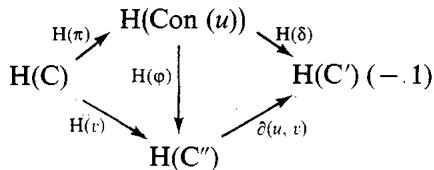
\includegraphics[keepaspectratio]{images/part001_82ee8f27.jpg}}

是可交换的，且H(φ)是双射。

在交换图（10）中，我们有 \(\mathrm{H}(1_{\mathbf{C}^{\prime}})\circ \partial (\tilde{u},\tilde{\pi}) = \partial (u,v)\circ \mathrm{H}(\varphi)\) （X，第31页，命题2）和 \(\partial (\tilde{u},\tilde{\pi}) = \mathrm{H}(\delta)\) （X，第38页，引理3，b）），因此

\[
\partial (u, v) \circ \mathbf {H} (\varphi) = \mathbf {H} (\delta);
\]

另一方面， \(\mathrm{H}(v) \circ \mathrm{H}(\beta) = \mathrm{H}(\varphi) \circ \mathrm{H}(\tilde{\pi}) = \mathrm{H}(\varphi) \circ \mathrm{H}(\pi) \circ \mathrm{H}(\beta)\) 根据X，第39页，注记。由于 \(\mathrm{H}(\beta)\) 是双射的，这给出 \(\mathrm{H}(v) = \mathrm{H}(\varphi) \circ \mathrm{H}(\pi)\) .

我们因此有 \(\partial(u, v) = H(\delta) \circ H(\varphi)^{-1}\) ，它为连接同态 \(\partial(u, v)\) 提供了一个新的定义。我们还注意到，如果把 \(H(Con(u))\) 与 \(H(C'')\) 借助 \(H(\varphi)\) 等同起来，则前面的推论表明，正合列（8）此时等同于相对于（9）的同调正合列。

\subsection{欧拉–庞加莱示性数}

在本节中，我们考虑一个由A-模的类组成的集合C，它是可加的且左正合的，即满足以下两个条件：

\begin{enumerate}
\def\labelenumi{(\Alph{enumi})}
\item
  若M和N是两个属于类型C的A-模，则M ⊕ N属于类型C。
\item
  若 \(0 \to \mathbf{M}' \to \mathbf{M} \to \mathbf{M}'' \to 0\) 是 A-模的一个正合列，且若 \(\mathbf{M}\) 与 \(\mathbf{M}''\) 属于类型 \(\mathcal{C}\) ，则 \(\mathbf{M}'\) 属于类型 \(\mathcal{C}\) .
\end{enumerate}

我们说 \(\mathcal{C}\) 是稳定的，如果它满足以下条件，这些条件蕴含(A)和(G)：

\begin{enumerate}
\def\labelenumi{(\Alph{enumi})}
\setcounter{enumi}{4}
\item
  （“C 在扩张下稳定。”）若 0 → M' → M → M'' → 0 是 A-模的短正合列，且 M' 与 M'' 属于 C 型，则 M 也属于 C 型。
\item
  （“C 在核与余核下稳定。”）对于类型 C 的 A-模的每个同态 f，A-模 Ker f 和 Coker f 均为类型 C。
\end{enumerate}

我们用 K( \(\mathcal{C}\) ) 表示 \(\mathcal{C}\) 的格罗滕迪克群，用 {[}M{]} \(_{\mathcal{C}}\) 或 {[}M{]} 表示由 A-模 M 定义的 K( \(\mathcal{C}\) ) 的元素（VIII，§ 6，第 2 节）。设 G 是一个交换群， \(\varphi\) 是从 K( \(\mathcal{C}\) ) 到 G 中的一个同态。

例子. --- 1) 若 A 是一个域，可取 C 为有限维向量空间的类组成的集合，并取 φ 为 K(C) 到 Z 上的同构，由 φ({[}M{]}) = dim (M) 定义。

\begin{enumerate}
\def\labelenumi{\arabic{enumi})}
\setcounter{enumi}{1}
\tightlist
\item
  可取 \(\mathcal{C}\) 为有限长度模的类构成的集合，并取 \(\varphi: \mathbf{K}(\mathcal{C}) \to \mathbf{Z}\) 为由 \(\varphi([\mathbf{M}]) = \text{long}_{\mathbf{A}}(\mathbf{M})\) 定义的同态。
\end{enumerate}

称分次A-模M为C型的，如果 \(M_{n}\) 对每个 n 而言都是 C 型的（为此，若 M 有界，则这是必要的；若 C 是稳定的，则这是充分的，即模 M 为 C 型）。

定义 8. --- 设 M 为一个 C 型的有界分次 A-模，并设 (M \(_{n}\) ) 为其分次。称 ∑ (-1) \(^{n}\) φ({[}M \(_{n}\) {]}) （G 的元素）为 M 的 φ-示性数，记作 χφ(M) 或简记为 χ(M)。

该定义特别适用于 M 是 A-模复形的底层分次模的情形。

例子. --- 3) 若 M 是 C 型有界的，则对每个 \(p \in Z\) ，M(p) 亦然，并且我们有 \(\chi(\mathbf{M}(p)) = (-1)^{p} \chi(\mathbf{M})\) .

\begin{enumerate}
\def\labelenumi{\arabic{enumi})}
\setcounter{enumi}{3}
\tightlist
\item
  设 \(0 \to \mathbf{M}' \to \mathbf{M} \to \mathbf{M}'' \to 0\) 是分次 A-模与次数为 0 的分次同态的一个正合列。若 \(\mathbf{M}, \mathbf{M}'\) 与 \(\mathbf{M}''\) 是 \(\mathcal{C}\) 型有界的，则我们有
\end{enumerate}

\[
\chi (\mathbf {M}) = \chi (\mathbf {M} ^ {\prime}) + \chi (\mathbf {M} ^ {\prime \prime}).
\]

如果 M 和 M'' 是类型 C 有界的，则 M' 亦然；如果 C 是稳定的，且三个模中有两个是类型 C 有界的，则第三个亦然。

\begin{enumerate}
\def\labelenumi{\arabic{enumi})}
\setcounter{enumi}{4}
\tightlist
\item
  设 \(u: \mathbf{C}' \to \mathbf{C}\) 是 \(\mathcal{C}\) 型有界复形的一个态射。则 Con \((u)\) 是 \(\mathcal{C}\) 型有界的，并且我们有：
\end{enumerate}

\[
\chi (\operatorname{Con} (u)) = \chi (\mathbf {C}) - \chi (\mathbf {C} ^ {\prime}).
\]

\begin{enumerate}
\def\labelenumi{\arabic{enumi})}
\setcounter{enumi}{5}
\tightlist
\item
  可将 G 取为群 K(C) 本身，并取 φ 为恒等映射；此时我们用 \(\chi_{\mathcal{C}}(\mathrm{M})\) 表示 K(C) 的元素 \(\chi_{\varphi}(\mathrm{M}) = \sum (-1)^{n}[\mathrm{M}_{n}]\) 。
\end{enumerate}

注记。--- 称相对于 \(\varphi\) 的元素 \(\mathrm{P}_{\mathbf{M}}(t) = \sum \varphi([\mathrm{M}_{n}]) t^{n} \in \mathrm{G} \otimes \mathbf{Z}[t, t^{-1}]\) 为 M 的庞加莱多项式。我们有 \(\mathrm{P}_{\mathbf{M}}(1) = \varphi([\mathrm{M}])\) 与 \(\mathrm{P}_{\mathbf{M}}(-1) = \chi(\mathrm{M})\) .

引理4. --- 设C是一个有界复形，类型为 \(\mathcal{C}\) 。如果 H(C) = 0，我们有 \(\chi(\mathbf{C}) = 0\) 这由第八卷，第6节，第1号，命题1的推论得出。

命题10. --- 设 C 和 C' 是两个 C 型有界复形。若存在一个拟同构 \(u: \mathbf{C}' \to \mathbf{C}\) ，则我们有 \(\chi(\mathbf{C}) = \chi(\mathbf{C}')\) .

确实，Con \((u)\) 是 \(\mathcal{C}\) 型有界的，并且我们有 \(\chi(\text{Con } (u)) = \chi(\text{C}) - \chi(\text{C}')\) ；另一方面，由 X，第 38 页，推论，H(Con \((u)) = 0\) ，因此 \(\chi(\text{Con } (u)) = 0\) （引理4）。

命题11. --- 设C是一个有界C型复形。

\begin{enumerate}
\def\labelenumi{\alph{enumi})}
\item
  若 \(\mathcal{C}\) 是稳定的，则 H(C) 是 \(\mathcal{C}\) 型的 .
\item
  如果 H(C) 是类型 C，那么 B(C) 和 Z(C) 也是，并且我们有 \(\chi(\mathrm{H}(\mathrm{C})) = \chi(\mathrm{C})\) .
\item
  若 \(\mathcal{C}\) 是稳定的，则对每个 \(n\) ，模 \(\mathbf{Z}_n(\mathbf{C})\) 是 \(\mathcal{C}\) 型的，作为 \(d_n: \mathbf{C}_n \to \mathbf{C}_{n-1}\) 的核；且 \(\mathrm{H}_n(\mathbf{C})\) 是 \(\mathcal{C}\) 型的，作为 \(\mathbf{C}_{n+1} \to \mathbf{Z}_n\) 的余核。另一方面， \(\mathrm{H}_n(\mathbf{C}) = 0\) （只要 \(\mathbf{C}_n = 0\) ）.
\item
  假设 H(C) 是 C 型的。典范正合列：
\end{enumerate}

\[
0 \to Z _ {n} (\mathbf {C}) \to C _ {n} \to B _ {n - 1} (\mathbf {C}) \to 0
\]

\[
0 \to \mathrm{B} _ {n} (\mathrm{C}) \to \mathrm{Z} _ {n} (\mathrm{C}) \to \mathrm{H} _ {n} (\mathrm{C}) \to 0
\]

从 C 的右界出发对 n 作归纳可知， \(Z_{n}(C)\) 与 \(B_{n}(C)\) 对每个 n 都是 C 型的。于是我们有

\[
\chi (\mathrm{C}) = \chi (\mathrm{Z} (\mathrm{C})) + \chi (\mathrm{B} (\mathrm{C}) (- 1)) = \chi (\mathrm{Z} (\mathrm{C})) - \chi (\mathrm{B} (\mathrm{C})) = \chi (\mathrm{H} (\mathrm{C})).
\]

推论。 --- 若 C 是稳定的且 C 是 C 型有界的，则分次模 H(C) 是 C 型有界的，并且我们有 \(\chi(\mathrm{H}(\mathrm{C})) = \chi(\mathrm{C})\) .

命题12. --- 设 \(0 \to C' \to C \to C'' \to 0\) 是复形的一个正合列。a) 若 H(C)、H(C') 和 H(C'') 是 C 型有界的，则我们有

\[
\chi (\mathrm{H} (\mathbf {C})) = \chi (\mathrm{H} (\mathbf {C} ^ {\prime})) + \chi (\mathrm{H} (\mathbf {C} ^ {\prime \prime})) .
\]

\begin{enumerate}
\def\labelenumi{\alph{enumi})}
\setcounter{enumi}{1}
\tightlist
\item
  如果C是稳定的，并且分次模H(C)、H(C')和H(C'')中有两个是C型有界的，那么第三个也是。
\end{enumerate}

a) 由将引理4应用于由所给正合列相关联的同调正合列所定义的零同调复形得出。b) 通过考虑该同调正合列，由以下引理得出：

引理5. --- 设 M → N → P → Q → R 是 A-模的正合列。若 C 是稳定的，且 M、N、Q 和 R 属于 C 型，则模 P 属于 C 型。

令 \(\mathbf{N}' = \operatorname{Coker} (\mathbf{M} \to \mathbf{N})\) 与 \(\mathbf{Q}' = \operatorname{Ker} (\mathbf{Q} \to \mathbf{R})\) 。模 \(\mathbf{N}'\) 与 \(\mathbf{Q}'\) 属于类型 \(\mathcal{C}\) ，并且我们有一个正合列 \(0 \to \mathbf{N}' \to \mathbf{P} \to \mathbf{Q}' \to 0\) .

推论。--- 假设 C 是稳定的，并设 \(u : C' \to C\) 是复形的一个态射，使得 \(\mathrm{H}(\mathbf{C})\) 与 \(\mathrm{H}(\mathbf{C}')\) 是 C 型有界的。则 \(\mathrm{H}(\mathrm{Con}(u))\) 是 C 型有界的，并且我们有

\[
\chi (\mathrm{H} (\text { Con } (u))) = \chi (\mathrm{H} (\mathrm{C})) - \chi (\mathrm{H} (\mathrm{C} ^ {\prime})) .
\]

这由命题 12 应用于复形的正合列（X，第 37 页，命题 7）得出

\[
0 \rightarrow \mathrm{C} \rightarrow \operatorname{Con} (u) \rightarrow \mathrm{C} ^ {\prime} (- 1) \rightarrow 0.
\]

注记。--- 设 E 是一个复形， \(h: \mathrm{E} \to \mathrm{C}\) 与 \(h': \mathrm{E} \to \mathrm{C}'\) 是同伦等价，其中 C 与 C' 是 \(\mathcal{C}\) 型有界的。则我们有 \(\chi(\mathrm{C}) = \chi(\mathrm{C}')\) 。事实上，若 \(h_1\) 是 \(h\) 在同伦意义下的逆，则 \(h' \circ h_1\) 是一个同伦等价，因此是从 C 到

C' 的一个拟同构，从而可以应用命题10。因此，只要存在从 E 到 C 型有界复形 C 的同伦等价，就可以通过设定 \(\chi(E) = \chi(C)\) 来扩展定义 8。命题 10、11、12 及其推论均可推广到这一情形。

应用：

* 设 X 是一个容许有限胞腔分解的拓扑空间（参见第 3 节）。a) 设 K 和 K' 是两个域，令 \(b_i = \dim_K(\mathrm{H}_i(\mathrm{X}, \mathrm{K}))\) 与 \(b_i' = \dim_K(\mathrm{H}_i(\mathrm{X}, \mathrm{K}'))\) 。我们不一定有 \(b_i = b_i'\) ，但有 \(\Sigma(-1)^i b_i = \Sigma(-1)^i b_i'\) .

\begin{enumerate}
\def\labelenumi{\alph{enumi})}
\setcounter{enumi}{1}
\tightlist
\item
  设 \((\mathbf{X}_{n})\) 与 \((\mathbf{X}_{n}^{\prime})\) 是 X 的两个有限胞腔分解，并设 \(c_{n}\) 与 \(c_{n}^{\prime}\) 是这两个分解中 n 维胞腔的个数。我们有
\end{enumerate}

\[
\Sigma (- 1) ^ {i} c _ {i} = \Sigma (- 1) ^ {i} c _ {i} ^ {\prime}.
\]

\begin{enumerate}
\def\labelenumi{\alph{enumi})}
\setcounter{enumi}{2}
\tightlist
\item
  利用 \(a)\) 与 \(b)\) 的记号，我们有 \(\Sigma(-1)^{i} c_{i} = \Sigma(-1)^{i} b_{i}\) .
\end{enumerate}

性质 \(a\) ) 与 \(b\) ) 由 \(c\) ) 推出，而 \(c\) ) 由命题11应用于第 3 号中所述的复形 \(\Gamma\) 得出，取 \(\mathscr{C}\) 为有限维 K-向量空间的类，取 \(\varphi\) 为由 \(\varphi([\mathrm{M}]) = \dim_{\mathrm{K}}(\mathrm{M})\) 定义的函数（X，第 40 页，例 1）。*

\subsection{右模复形，多模复形}

右A-模的复形是一个分次右A-模 \((M_{n})_{n\in\mathbf{Z}}\) 配备了一个次数为-1且平方为零的分次自同态；因此它是环A°（与A相反）上的模复形。因此，前面各节所述的所有定义和性质都适用于右模复形，这些右模复形被视为环A°上的模复形。

类似地，若 A 和 B 是两个环，则 (A, B)-双模复形是配备有一个分次自同态 \(d\) （次数为 \((-1)\) 且平方为零）的分次 (A, B)-双模 M；若赋予 M 其作为左 A \(\otimes_{\mathbf{z}} \mathbf{B}^{\circ}\) -模的典范结构，则 \(d\) 赋予它一个 A \(\otimes_{\mathbf{z}} \mathbf{B}^{\circ}\) -复形的结构。因此，前面各节中陈述的所有定义和性质均适用于双模复形。多模复形的定义类似。

\subsection{例子：德拉姆复形}

在本节中，我们假设 A 是交换环 \(k\) 上的一个交换 \(k\) -代数。用 \(\Omega_{\mathbf{A}/k}^{1}\) 表示 A 的凯勒微分 A-模（III，第 134 页），用 \(d^{0}: \mathbf{A} \to \Omega_{\mathbf{A}/k}^{1}\) 表示 \(k\) -导子 \(d_{\mathbf{A}/k}\) ，并用 \(\Omega_{\mathbf{A}/k}\) 表示分次 \(k\) -代数 \(\boldsymbol{\Lambda}_{\mathbf{A}}(\Omega_{\mathbf{A}/k}^{1})\) .

命题13. --- 存在唯一的次数为 1、平方为零的 k-反导子 \(d: \Omega_{\mathbf{A}/k} \to \Omega_{\mathbf{A}/k}\) ，它延拓导子 \(d^{0}: \mathbf{A} \to \Omega_{\mathbf{A}/k}^{1}\) .

让我们证明反导子 \(d\) 的唯一性。由于 \(d \circ d = 0\) ，我们有，对于 \(y, x_1, \ldots, x_p \in \mathbf{A}\) :

\[
d \left(y d x _ {1} \wedge \dots \wedge d x _ {p}\right) = d y \wedge d x _ {1} \wedge \dots \wedge d x _ {p}.
\]

A-模 \(\Omega_{\mathbf{A}/k}^{p}\) 由元素 \(dx_{1} \wedge \ldots \wedge dx_{p}\) 生成，这就证明了 \(d\) 的唯一性 .

为了证明存在性，只需构造一个 \(k\) -同态 \(d^{1}:\Omega_{\mathbb{A}/k}^{1}\to\Omega_{\mathbb{A}/k}^{2}\) ，使得 \(d^{1}\circ d^{0}=0\) 且

\[
d ^ {1} (a \omega) = d ^ {0} (a) \wedge \omega + a d ^ {1} (\omega) \quad \text {for} \quad a \in A, \quad \omega \in \Omega_ {A k} ^ {1}.\tag{11}
\]

事实上，由 III，第 128 页，命题 14（考虑到 III，第 118 页，注记 2）可知，存在一个反导子 \(d: \Omega_{\mathbf{A}/k} \to \Omega_{\mathbf{A}/k}\) ，它在次数为 0 时与 \(d^{0}\) 重合，在次数为 1 时与 \(d^{1}\) 重合。由于 \(d^{0}\) 在 \(\mathbf{A}\) 上为零，反导子 \(d\) 是 \(k\) -线性的；由于 \(d^{1} \circ d^{0} = 0\) ，我们有 \(d \circ d = 0\) ，因为 \(\Omega_{\mathbf{A}/k}\) 作为 \(\mathbf{A}\) -代数由元素 \(d^{0} a\) （ \(a \in \mathbf{A}\) ）生成 .

为了定义 \(d^{1}\) ，回顾（III，第 133 页） \(\Omega_{\mathbf{A}/k}^{1}\) 等于 A-模 \(\mathfrak{I}/\mathfrak{I}^{2}\) ，其中 \(\mathfrak{I}\) 是乘法 \(m: \mathbf{A} \otimes_{k} \mathbf{A} \to \mathbf{A}\) 的核。考虑 \(k\) -线性映射 \(u: \mathbf{A} \otimes_{k} \mathbf{A} \to \Omega_{\mathbf{A}/k}^{2}\) ，它由 \(u(x \otimes y) = d^{0}(y) \wedge d^{0}(x)\) 定义。我们有

\[
u (a x \otimes y - x \otimes a y) = d ^ {0} (y) \wedge d ^ {0} (a x) - d ^ {0} (a y) \wedge d ^ {0} (x) = d ^ {0} (x y) \wedge d ^ {0} (a)
\]

对于 A 中的 x、y 和 a，由此可得

\[
u ((a \otimes 1 - 1 \otimes a) \xi) = d ^ {0} (m (\xi)) \wedge d ^ {0} (a), \quad \xi \in \mathrm{A} \otimes_ {k} \mathrm{A}, \quad a \in \mathrm{A}. \tag {12}
\]

由于 \(\mathfrak{I}\) 作为左 A-模由元素 ( \(a \otimes 1 - 1 \otimes a\) ) （ \(a \in \mathbf{A}\) ）生成，我们推出 \(u(\mathfrak{I}^2) = 0\) ；因此 \(u\) 通过限制到 \(\mathfrak{I}\) 并过渡到商，定义了一个 \(k\) -线性映射 \(d^1: \mathfrak{I}/\mathfrak{I}^2 \to \Omega_{\mathrm{A}/k}^2\) .

在（12）中取 \(\xi = b \otimes 1\) （其中 \(b \in \mathbf{A}\) ），我们得到 \(d^{1}(bd^{0}(a)) = d^{0}(b) \wedge d^{0}(a)\) ；由此得出 \(d^{1} \circ d^{0} = 0\) ，以及 \(d^{1}(c\omega) = d^{0}(c) \wedge \omega + cd^{1}(\omega)\) （对 \(c \in \mathbf{A}\) 与 \(\omega = bd^{0}(a)\) ）。由于 \(\Omega_{\mathbf{A}/k}^{1}\) 作为 \(k\) -模由元素 \(bd^{0}(a)\) （ \(a\) 与 \(b\) 属于 \(\mathbf{A}\) ）生成，公式（11）对所有 \(\omega \in \Omega_{\mathbf{A}/k}\) 成立，这就完成了命题的证明。

有时称元素 \(\omega\in\Omega_{A/k}^{p}\) 为次数为 \(p\) 的外微分形式（A 在 \(k\) 上），并称反导子 \(d\) 为 \(\Omega_{A/k}\) 的外微分；复形（ \(\Omega_{A/k}\) , \(d\) ）称为 A 在 \(k\) 上的德拉姆复形，其同调为 A 在 \(k\) 上的德拉姆上同调 .

例 1. --- 取 A 为环 \(k[\mathbf{X}_{1},\ldots,\mathbf{X}_{n}]\) 。则 \(\Omega_{\mathbf{A}/k}^{1}\) 是一个自由 A-模，其基为 \(d\mathbf{X}_{1},\ldots,d\mathbf{X}_{n}\) （III，第 134 页，例）。因此，若对每个子集 \(\mathrm{I}=\{i_{1},\ldots,i_{p}\}\) （ \([1,n]\) 的）设 \(d\mathbf{X}_{\mathrm{I}}=d\mathbf{X}_{i_{1}}\wedge\ldots\wedge d\mathbf{X}_{i_{p}}\) （其中 \(i_{1}<\ldots<i_{p}\) ），则 A-模 \(\Omega_{\mathbf{A}/k}^{p}\) 以元素 \(d\mathbf{X}_{\mathrm{I}}\) 为基，其中 I 遍历 \([1,n]\) 的基数为 \(p\) 的子集的集合。我们有

\[
d (\mathrm{P} d \mathrm{X} _ {\mathrm{I}}) = d \mathrm{P} \wedge d \mathrm{X} _ {\mathrm{I}} = \sum_ {i \notin \mathrm{I}} (- 1) ^ {n (\mathrm{I}, i)} \frac {\partial \mathrm{P}}{\partial \mathrm{X} _ {i}} d \mathrm{X} _ {\mathrm{I} \cup \{i \}},
\]

其中 \(n(\mathbf{I}, i)\) 表示 I 中严格小于 \(i\) 的元素的个数 .

\(Z^{p}(\Omega_{\mathbf{A}/k})\) 的闭链因此是这样的元素 \(\omega = \sum_{\text{Card (I)} = p} \mathrm{P}_{\mathrm{I}} d\mathrm{X}_{\mathrm{I}}\) ：对每个子集 \(J\) （含 \((p + 1)\) 个元素，属于 \([1, n]\) ），有：

\[
\sum_ {i \in J} (- 1) ^ {n (J, i)} \frac {\partial P _ {J - \{i \}}}{\partial X _ {i}} = 0.
\]

元素 ω 是一个边缘，如果对于每个子集 \(J \subset [1, n]\) （含 \((p - 1)\) 个元素），可以选择一个多项式 \(Q_{J} \in A\) ，使得：

\[
\mathrm{P} _ {\mathrm{I}} = \sum_ {j \in \mathrm{I}} (- 1) ^ {n (\mathrm{I}, j)} \frac {\partial \mathrm{Q} _ {\mathrm{I} - \{j \}}}{\partial \mathrm{X} _ {j}}.
\]

我们将在 § 9 中看到，如果 k 是一个 Q-代数，则 A 在 k 上的德拉姆复形在次数 \textgreater{} 0 上是零调的（X，第 159 页，注记 4）。

* 例 2. --- 假设 \(k = \mathbf{C}\) 且 \(\mathbf{A} = \mathbf{C}\) \([\mathrm{X}_1, \ldots, \mathrm{X}_n] / (\mathrm{P}_1, \ldots, \mathrm{P}_r)\) ，其中 \(\mathrm{P}_i\) 是 \(\mathrm{X}_1, \ldots, \mathrm{X}_n\) 的多项式，使得 \(\mathbf{C}^n\) 中所有 \(\mathrm{P}_i\) 为零的点集是 \(\mathbf{C}^n\) 的一个解析子流形 V。可以证明 A 在 C 上的德拉姆上拟同构于奇异上同调 H(V, C)。*

设 M 是一个 A-模，且 \(\nabla^{0}\) 为 \(k\) -线性映射，从 M 到 \(\mathbf{M} \otimes_{\mathbf{A}} \Omega_{\mathbf{A}/k}^{1}\) 使得

\[
\nabla^ {0} (a m) = a \nabla^ {0} (m) + m \otimes d a \quad \text { for } \quad a \in \mathrm{A}, \quad m \in \mathrm{M}\tag{13}
\]

（有时也称 \(\nabla^{0}\) 为 A-模 M 上的一个联络）。

命题 14. --- (i) 存在唯一的 k-线性映射 \(\nabla\) 从 \(\Omega_{\mathbf{A}/k}\) 右模 \(\mathbf{M} \otimes_{\mathbf{A}} \Omega_{\mathbf{A}/k}\) 到自身，次数为 1 的分次映射，它扩展了 \(\nabla^{0}\) 在次数0中，并满足恒等式：

\[
\nabla (x \omega) = (\nabla x) \omega + (- 1) ^ {p} x (d \omega) \quad \mathrm{for} \quad x \in \mathrm{M} \otimes_ {\mathrm{A}} \Omega_ {\mathrm{A} / k} ^ {p}, \quad \omega \in \Omega_ {\mathrm{A} / k}. \tag {14}
\]

\begin{enumerate}
\def\labelenumi{(\roman{enumi})}
\setcounter{enumi}{1}
\tightlist
\item
  复合映射 \(\nabla \circ \nabla\) 是 \(\Omega_{\mathbf{A} / k}\) -线性；特别地，映射 \(\mathbf{R} = \nabla^{1} \circ \nabla^{0}\) 的 \(\mathbf{M}\) 到 \(\mathbf{M} \otimes_{\mathbf{A}} \Omega_{\mathbf{A} / k}^{2}\) 是 \(\mathbf{A}\) -线性，并且我们有
\end{enumerate}

\[
\nabla \circ \nabla (m \otimes \omega) = R (m). \omega \quad \mathrm{for} \quad m \in M, \quad \omega \in \Omega_ {A / k}.
\]

同态 R 有时称为联络 \(\nabla^{0}\) 的曲率同态；若它为零，则偶对 \((\mathbf{M} \otimes_{\mathbf{A}} \Omega_{\mathbf{A}/k}, \nabla)\) 是一个复形，也称为 \((\mathbf{M}, \nabla^{0})\) 在 \(k\) 上的德拉姆复形 .

我们来证明 (i)。 \(\nabla\) 的唯一性是显然的。让我们定义一个 \(k\) -同态 \(\overline{\nabla}\) ，从 \(\mathbf{M} \otimes_k \Omega_{\mathbf{A}/k}\) 到 \(\mathbf{M} \otimes_{\mathbf{A}} \Omega_{\mathbf{A}/k}\) ：

\[
\overline {{{\nabla}}} (m \otimes_ {k} \omega) = (\nabla^ {0} m) \omega + m \otimes d \omega \quad \text { for } \quad m \in \mathbf {M}, \quad \omega \in \Omega_ {\mathrm{A} / k}.
\]

由（13）可得 \(\overline{\nabla}(am \otimes \omega) = \overline{\nabla}(m \otimes a\omega)\) ，因此通过过渡到商，我们得到一个 \(k\) -同态 \(\nabla\) ，它从 \(\mathbf{M} \otimes_{\mathbf{A}} \Omega_{\mathbf{A}/k}\) 到自身、次数为 1 的分次映射，且在次数 0 时延拓 \(\nabla^{0}\) 。让我们验证（14）：我们有，对于 \(m \in \mathbf{M}\) , \(\alpha \in \Omega_{\mathbf{A}/k}^{p}\) , \(\omega \in \Omega_{\mathbf{A}/k}\) :

\[
\begin{array}{r l} \nabla ((m \otimes \alpha). \omega) & = \nabla (m \otimes (\alpha \wedge \omega)) = \nabla^ {0} (m). (\alpha \wedge \omega) + m \otimes d (\alpha \wedge \omega) \\ & = \nabla^ {0} (m) \alpha . \omega + (m \otimes d \alpha) \omega + (- 1) ^ {p} (m \otimes \alpha) d \omega \\ & = (\nabla (m \otimes \alpha)) \omega + (- 1) ^ {p} (m \otimes \alpha) d \omega \end{array}
\]

这证明了 (14) 式对 \(x = m \otimes \alpha\) 成立；一般情形由此通过线性性推出。

让我们证明(ii)。设 \(x \in \mathbf{M} \otimes_{\mathbf{A}} \Omega_{\mathbf{A}/k}^{p}\) , \(\omega \in \Omega_{\mathbf{A}/k}\) ；通过反复应用(14)，我们得到：

\[
\begin{array}{r l} \nabla \circ \nabla (x \omega) = & \nabla (\nabla (x) \omega) + (- 1) ^ {p} \nabla (x d \omega) \\ & = (\nabla \circ \nabla (x)) \omega + (- 1) ^ {p + 1} \nabla (x) (d \omega) + (- 1) ^ {p} \nabla (x) (d \omega) \\ & = (\nabla \circ \nabla (x)) \omega , \end{array}
\]

这证明了(ii)的第一个断言；其余断言随之立即成立。

\section{分解}

我们沿用上一节的约定。

\subsection{复形态射的扩张}

引理1. --- 考虑一个由A-模及同态构成的图表

\[
\begin{array}{c} \mathbf {M} ^ {\prime} \xrightarrow {\alpha^ {\prime}} \mathbf {M} \xrightarrow {\alpha} \mathbf {M} ^ {\prime \prime} \\ f ^ {\prime} \Biggl \downarrow \quad \swarrow k / f \Biggl \downarrow \quad \swarrow k ^ {\prime \prime} \\ \mathbf {N} ^ {\prime} \xrightarrow [ \beta^ {\prime} ]{} \mathbf {N} \xrightarrow [ \beta ]{} \mathbf {N} ^ {\prime \prime} \end{array}
\]

使得 \(f \circ \alpha' = \beta \circ f', \alpha \circ \alpha' = 0\) ，Ker \(\beta = \operatorname{Im} \beta'\) ，且 \(f = k'' \circ \alpha + \beta \circ k\) 且其中 \(\mathbf{M}'\) 是投射的。存在一个A-同态 \(k': \mathbf{M}' \to \mathbf{N}'\) 使得 \(f' = k \circ \alpha' + \beta' \circ k'\) .

事实上，令 \(g = f' - k \circ \alpha'\) ；我们有

\[
\beta \circ g = \beta \circ f ^ {\prime} - \beta \circ k \circ \alpha^ {\prime} = f \circ \alpha^ {\prime} - \beta \circ k \circ \alpha^ {\prime} = k ^ {\prime \prime} \circ \alpha \circ \alpha^ {\prime} = 0.
\]

这意味着 \(\operatorname{Im}(g) \subset \operatorname{Ker}(\beta) = \operatorname{Im}(\beta')\) 。由于 \(\mathbf{M}'\) 是投射的，因此存在一个A-同态 \(k': \mathbf{M}' \to \mathbf{N}'\) 使得 \(\beta' \circ k' = g\) ，从而引理得证。

引理2. --- 如果在A-模与同态的交换图中

\[
\begin{array}{c c c c c} \mathbf {M} ^ {\prime} & \xrightarrow {\alpha^ {\prime}} & \mathbf {M} & \xrightarrow {\alpha} & \mathbf {M} ^ {\prime \prime} \\ & & \Big \downarrow^ {u} & & \Big \downarrow^ {u ^ {\prime \prime}} \\ \mathbf {N} ^ {\prime} & \xrightarrow {\beta^ {\prime}} & \mathbf {N} & \xrightarrow {\beta} & \mathbf {N} ^ {\prime \prime} \end{array}
\]

我们有 \(\alpha\circ\alpha'\) =0，Ker \(\beta=\operatorname{Im}\beta'\) 且如果 \(\mathbf{M}'\) 是投射的，则存在一个A-同态 \(u':\mathbf{M}'\to\mathbf{N}'\) 使得 \(\beta'\circ u'=u\circ\alpha'\) .

只需在引理1中设 \(k'' = u'', k = -u, f = 0, f' = 0\) 与 \(u' = k'\) 即可。

引理1 bis. --- 考虑一个A-模与同态的图表

\[
\begin{array}{c} \mathbf {M} ^ {\prime} \xrightarrow {\alpha^ {\prime}} \mathbf {M} \xrightarrow {\alpha} \mathbf {M} ^ {\prime \prime} \\ \Big \downarrow_ {k ^ {\prime}} \Big \downarrow_ {f ^ {\prime}} \Big \downarrow_ {k} \Big \downarrow_ {f} \\ \mathbf {N} ^ {\prime} \xrightarrow [ \beta^ {\prime} ]{} \mathbf {N} \xrightarrow [ \beta ]{} \mathbf {N} ^ {\prime \prime} \end{array}
\]

使得 \(f \circ \alpha' = \beta \circ f'\) ，Ker \(\alpha = \operatorname{Im} \alpha'\) , \(\beta \circ \beta' = 0\) ，且 \(f' = k \circ \alpha' + \beta' \circ k'\) ，且其中 \(N''\) 是单射的。存在一个 A-同态 \(k'' : M'' \to N''\) 使得 \(f = k'' \circ \alpha + \beta \circ k\) 。事实上，设 \(q = f - \beta \circ k\) ，我们有

\[
g \circ \alpha^ {\prime} = f \circ \alpha^ {\prime} - \beta \circ k \circ \alpha^ {\prime} = \beta \circ f ^ {\prime} - \beta \circ k \circ \alpha^ {\prime} = \beta \circ \beta^ {\prime} \circ k ^ {\prime} = 0.
\]

这蕴含Ker \(g \supset \operatorname{Im} \alpha' = \operatorname{Ker} \alpha\) 。由于 \(\mathbf{N}''\) 是单射的，因此（X，第16页，注记）存在一个A-同态 \(k': \mathbf{M}'' \to \mathbf{N}''\) 使得 \(g = k'' \circ \alpha\) ，从而引理得证。

引理2 bis. --- 若在A-模与同态的交换图中

\[
\begin{array}{c c c c c} \mathbf {M} ^ {\prime} & \stackrel {{\alpha^ {\prime}}} {{\longrightarrow}} & \mathbf {M} & \stackrel {{\alpha}} {{\longrightarrow}} & \mathbf {M} ^ {\prime \prime} \\ u ^ {\prime} \Big \downarrow & & u \Big \downarrow & & \\ \mathbf {N} ^ {\prime} & \stackrel {{\beta^ {\prime}}} {{\longrightarrow}} & \mathbf {N} & \stackrel {{\beta}} {{\longrightarrow}} & \mathbf {N} ^ {\prime \prime}, \end{array}
\]

我们有 \(\operatorname{Ker} \alpha = \operatorname{Im} \alpha'\) , \(\beta \circ \beta' = 0\) 且如果 \(\mathbf{N}''\) 是单射的，则存在一个A-同态 \(u'' : \mathbf{M}'' \to \mathbf{N}''\) 使得 \(u'' \circ \alpha = \beta \circ u\) .

只需在引理 1 bis 中设 \(u' = k', u = -k, f = 0, f' = 0\) 与 \(k'' = u''\) 即可。

命题1. --- 设(P, \(d_{\mathbb{P}}\) ) 和 (E, \(d_{\mathbb{E}}\) ) 是 A-模的两个复形，且 r 是一个整数。

\begin{enumerate}
\def\labelenumi{\alph{enumi})}
\item
  设 \((u_i: \mathrm{P}_i \to \mathrm{E}_i)_{i \leqslant r}\) 是一个同态族，使得 \(d_{\mathrm{E}} \circ u_i = u_{i-1} \circ d_P\) （对 \(i \leqslant r\) ）。假设 \(\mathrm{P}_i\) 对 \(i > r\) 是投射的，且 \(\mathrm{H}_i(\mathrm{E}) = 0\) （对 \(i \geqslant r\) ）。则 \(u_i\) 的族可延拓为从 P 到 E 的一个复形态射；两个这样的延拓是同伦的。
\item
  设 \((u^{i}:\mathbf{P}^{i}\to\mathbf{E}^{i})_{i\leqslant r}\) 是一个同态族，使得 \(u^{i}\circ d_{\mathrm{P}}=d_{\mathrm{E}}\circ u^{i-1}\) （对 \(i\leqslant r\) ）。假设 \(\mathbf{E}^{i}\) 对 \(i>r\) 是单射的，且 \(\mathbf{H}^{i}(\mathbf{P})=0\) （对 \(i\geqslant r\) ）。则 \(u^{i}\) 的族可延拓为从 \(\mathbf{P}\) 到 \(\mathbf{E}\) 的一个复形态射；两个这样的延拓是同伦的。
\end{enumerate}

让我们证明 a)。族 \((u_{i})_{i\leqslant r}\) 的一个扩张 v 的存在性由引理 2 通过归纳法直接得出。设 \(v'\) 是另一个扩张；设 \(f=v'-v\) ，并对整数 n 作归纳，构造一个同态 \(k_{n}:P_{n}\to E_{n+1}\) ，使得 \(f_{n}=d_{E}\circ k_{n}+k_{n-1}\circ d_{P}\) 。对 \(i\leqslant r\) ，取 \(k_{i}=0\) 。设 \(n\geqslant r\) 并假设 \(k_{i}\) 对 \(i\leqslant n\) 已构造。于是考虑图表

\[
\begin{array}{c} \mathrm{P} _ {n + 1} \xrightarrow {d _ {\mathrm{p}}} \mathrm{P} _ {n} \xrightarrow {d _ {\mathrm{p}}} \mathrm{P} _ {n - 1} \\ f _ {n + 1} \Biggl \downarrow \quad k _ {n} \Biggl \downarrow f _ {n} \Biggl \downarrow k _ {n - 1} \\ \mathrm{E} _ {n + 2} \xrightarrow {d _ {\mathrm{E}}} \mathrm{E} _ {n + 1} \xrightarrow {d _ {\mathrm{E}}} \mathrm{E} _ {n}. \end{array}
\]

引理1的假设得到满足；因此存在一个A-同态 \(k_{n+1}: \mathbf{P}_{n+1} \to \mathbf{E}_{n+2}\) 使得 \(f_{n+1} = d_{\mathbf{E}} \circ k_{n+1} + k_n \circ d_p\) ，从而 \(a\) ).

b) 的证明类似，借助引理 1 bis 与引理 2 bis 完成。

\subsection{分解}

在下文中，总是将模与一个复形等同起来，该复形以该模为零次分量，且所有其他分量为零。

定义1. --- 设 M 为一个 A-模。M 的一个左分解是一个偶对 (P, p)，其中 P 是一个在右侧为零的复形，且 p : P → M 是一个拟同构。M 的一个右分解是一个偶对 (e, E)，其中 E 是一个在左侧为零的复形，且 e : M → E 是一个拟同构。

称分解(P, p)（相应地(e, E)）的长度为复形P（相应地E）的长度。若(P, p)和(P', p')（相应地(e, E)和(e', E')）是M的两个左（相应地右）分解，则一个复形态射 \(f: P \to P'\) 使得 \(p' \circ f = p\) (相应地， \(g: E \to E'\) 使得 \(g \circ e = e'\) ）被称为分解的态射。

命题2. --- 设 P 为一个在右侧为零的复形，且设 p : P → M 为一个态射。要使 (P, p) 成为 M 的一个左分解，必要且充分条件是序列

\[
\dots \longrightarrow \mathrm{P} _ {n} \xrightarrow {d _ {\mathrm{P}}} \mathrm{P} _ {n - 1} \longrightarrow \dots \quad \longrightarrow \mathrm{P} _ {1} \xrightarrow {d _ {\mathrm{P}}} \mathrm{P} _ {0} \xrightarrow {p _ {0}} \mathrm{M} \longrightarrow 0\tag{1}
\]

是正合的。

事实上，说 \(p: \mathbf{P} \to \mathbf{M}\) 是拟同构，意味着 \(\mathrm{H}_{i}(\mathbf{P}) = 0\) （对 \(i > 0\) ），且 \(p_{0}\) 诱导了从 Coker ( \(d_{\mathbf{P}}: \mathbf{P}_{1} \to \mathbf{P}_{0}\) ) 到 \(\mathbf{M}\) 上的一个同构 .

的同构。类似地：

命题2bis. --- 设 E 是一个在左侧为零的复形，并设 e : M → E 是一个态射。要使 (e, E) 成为 M 的一个右分解，必要且充分条件是序列

\[
0 \longrightarrow \mathrm{M} \stackrel {e _ {0}} {\longrightarrow} \mathrm{E} ^ {0} \stackrel {d _ {\mathrm{E}}} {\longrightarrow} \mathrm{E} ^ {1} \longrightarrow \dots \longrightarrow \mathrm{E} ^ {n} \stackrel {d _ {\mathrm{E}}} {\longrightarrow} \mathrm{E} ^ {n + 1} \longrightarrow \dots\tag{1 bis}
\]

是正合的。

为方便起见，人们常说序列 (1)（相应地 (1 bis)）是 M 的左（相应地右）分解。

定义2. --- A-模 M 的一个投射（相应地自由、相应地平坦）分解是 M 的一个左分解 (P, p)，使得复形 P 是投射的（相应地自由的、相应地平坦的）（X，第 25 页）。M 的一个内射分解是 M 的一个右分解 (e, E)，使得复形 E 是内射的（同上）。

例子. --- 1) 假设环 A 是主理想整环；设 M 是一个 A-模，并设 \((x_{i})_{i\in I}\) 是 M 的一个生成族。设 \(L_{0}\) 是自由模 \(\mathbf{A}^{(I)}\) , \((e_{i})\) 为其典范基，并定义 \(p:L_{0}\to\mathbf{M}\) 为 \(p(e_{i})=x_{i}\) 。态射 \(p\) 是满射的，且其核 \(L_{1}\) 由 VII, § 3, 定理 1 的推论 2 知是一个自由 A-模，因此正合列

\[
0 \to \mathrm{L} _ {1} \to \mathrm{L} _ {0} \xrightarrow {p} \mathrm{M} \to 0
\]

是 M 的长度为 1 的自由分解。若 I 是有限的，则 \(L_{0}\) 与 \(L_{1}\) 是有限生成的。

\begin{enumerate}
\def\labelenumi{\arabic{enumi})}
\setcounter{enumi}{1}
\tightlist
\item
  假设 A 是交换的；设 E 是一个 A-模，u 是 E 的一个自同态。记 \(E_{u}\) 为通过赋予 E 由下式定义的结构而得到的 A{[}X{]}-模
\end{enumerate}

\[
(p, x) \mapsto p (u) (x) \quad \text { for } \quad p \in \mathrm{A} [ \mathrm{X} ] \quad \text { and } \quad x \in \mathrm{E}.
\]

根据III，第106页，我们有一个正合列：

\[
0 \to \mathrm{A} [ \mathrm{X} ] \otimes_ {\mathrm{A}} \mathrm{E} \stackrel {\psi} {\to} \mathrm{A} [ \mathrm{X} ] \otimes_ {\mathrm{A}} \mathrm{E} \stackrel {\varphi} {\to} \mathrm{E} _ {u} \to 0
\]

其中 \(\varphi(p \otimes x) = p.x\) 与 \(\psi(p \otimes x) = Xp \otimes x - p \otimes u(x)\) （当 \(p \in A[X]\) 与 \(x \in E\) ）。这个正合列是 \(E_u\) 的长度为 1 的自由（相应地，投射，相应地，有限生成）分解，如果 E 是自由（相应地，投射，相应地，有限生成）A-模。3) 如果 A 是主理想整环，则正合列

\[
0 \rightarrow \mathrm{A} \rightarrow \mathrm{K} \rightarrow \mathrm{K/A} \rightarrow 0
\]

是 A-模 \(\mathbf{A}_s\) 的长度为 1 的内射分解（X，第 18 页，例 1）。

命题 3. --- 设 \(f: \mathbf{M}' \to \mathbf{M}\) 是 A-模的一个同态， \(p': \mathbf{P}' \to \mathbf{M}'\) 是到 \(\mathbf{M}'\) 的、来自一个在右侧为零且投射的复形 \(\mathbf{P}'\) 的一个态射，且 \(p: \mathbf{P} \to \mathbf{M}\) 是 M 的一个左分解。存在一个复形态射 \(\tilde{f}: \mathbf{P}' \to \mathbf{P}\) ，且在同伦意义下唯一，使得 \(p \circ \tilde{f} = f \circ p'\) .

考虑如下定义的复形 \(\overline{\mathbf{P}}\) ： \(\overline{\mathbf{P}}_n = \mathbf{P}_n\) 当 \(n \neq -1\) , \(\overline{\mathbf{P}}_{-1} = \mathbf{M}\) , \(d_{\overline{\mathbf{P}},n} = d_{\mathbf{P},n}\) 当 \(n \neq 0, -1\) , \(d_{\overline{\mathbf{P}},0} = p_0\) , \(d_{\overline{\mathbf{P}},-1} = 0\) ，以及类似定义的复形 \(\overline{\mathbf{P}}'\) 。将命题 1 a) 应用于复形 \(\overline{\mathbf{P}}\) 与 \(\overline{\mathbf{P}}'\) ，取 \(r=0\) , \(u_i = 0\) （当 \(i < -1\) ）与 \(u_{-1} = f\) ，我们得到命题 3。

推论。--- 设 (P, p) 与 (P', p') 是 M 的两个投射分解。存在一个在同伦意义下唯一的同伦等价 \(\alpha: P' \to P\) ，使得 \(p \circ \alpha = p'\) .

事实上，存在一个态射 \(\alpha: P' \to P\) (相应地， \(\beta: P \to P'\) ）使得 \(p \circ \alpha = p'\) (相应地， \(p' \circ \beta = p\) ）。由于 \(p \circ \alpha \circ \beta = p\) (相应地， \(p' \circ \beta \circ \alpha = p'\) ), \(\alpha \circ \beta\) 同伦于 \(1_P\) (相应地， \(\beta \circ \alpha\) 同伦于 \(1_{P'}\) ).

命题 3 bis. --- 设 \(g: \mathbf{N} \to \mathbf{N}'\) 是 A-模的一个同态， \(e': \mathbf{N}' \to \mathbf{E}'\) 是 \(\mathbf{N}'\) 到一个在左侧为零且内射的复形 \(\mathbf{E}'\) 中的态射，且 \(e: \mathbf{N} \to \mathbf{E}\) 是 \(\mathbf{N}\) 的一个右分解。存在一个复形态射 \(\tilde{g}: \mathbf{E} \to \mathbf{E}'\) ，且在同伦意义下唯一，使得 \(\tilde{g} \circ e = e' \circ g\) .

此证明类似于命题3，借助命题1 b) 完成。

推论。--- 设 \((e, E)\) 与 \((e', E')\) 是 N 的两个内射分解；存在一个同伦等价 \(\alpha : E \to E'\) ，且在同伦意义下唯一，使得 \(\alpha \circ e = e'\) .

\subsection{典范自由分解}

对每个 A-模 M，用 \(\mathbf{L}_{0}(\mathbf{M})\) 表示以 M 为基的自由 A-模 \(\mathbf{A}^{(\mathbf{M})}\) ， \((e_{m})_{m\in\mathbf{M}}\) 为其典范基， \(p_{\mathbf{M}}:\mathbf{L}_{0}(\mathbf{M})\to\mathbf{M}\) 为使得

\[
p _ {\mathbf {M}} (e _ {m}) = m, \quad m \in \mathbf {M}.
\]

令 \(Z_0(\mathbf{M}) = \operatorname{Ker} p_{\mathbf{M}}\) 并设 \(i_{\mathbf{M}}: Z_0(\mathbf{M}) \to L_0(\mathbf{M})\) 为典范嵌入。我们有一个正合列

\[
0 \longrightarrow Z _ {0} (\mathrm{M}) \stackrel {i _ {\mathrm{M}}} {\longrightarrow} L _ {0} (\mathrm{M}) \stackrel {p _ {\mathrm{M}}} {\longrightarrow} \mathrm{M} \longrightarrow 0.\tag{1}
\]

我们通过如下设定来定义分次模 L(M)： \(\mathrm{L}_{n}(\mathrm{M}) = 0\) （当 n \textless{} 0），并对整数 n \textgreater{} 0 作归纳

\[
\mathrm{L} _ {n} (\mathrm{M}) = \mathrm{L} _ {0} \left(\mathrm{Z} _ {n - 1} (\mathrm{M})\right); \quad \mathrm{Z} _ {n} (\mathrm{M}) = \mathrm{Z} _ {0} \left(\mathrm{Z} _ {n - 1} (\mathrm{M})\right).\tag{2}
\]

我们定义 A-同态 \(d_{n}^{\mathbf{M}}:\mathrm{L}_{n}(\mathbf{M})\to \mathrm{L}_{n - 1}(\mathbf{M})\) 如下

\[
\left\{ \begin{array}{l l} d _ {n} ^ {\mathbf {M}} = 0, & n \leqslant 0, \\ d _ {1} ^ {\mathbf {M}} = i _ {\mathbf {M}} \circ p _ {\mathbf {Z} _ {0} (\mathbf {M})}, & \\ d _ {n} ^ {\mathbf {M}} = i _ {\mathbf {Z} _ {n - 2} (\mathbf {M})} \circ p _ {\mathbf {Z} _ {n - 1} (\mathbf {M})}, & n > 1. \end{array} \right.\tag{3}
\]

由构造，我们有一个正合列

\[
\longrightarrow \mathrm{L} _ {n} (\mathrm{M}) \xrightarrow {d _ {n} ^ {\mathrm{M}}} \mathrm{L} _ {n - 1} (\mathrm{M}) \longrightarrow \dots \longrightarrow \mathrm{L} _ {0} (\mathrm{M}) \xrightarrow {p _ {\mathrm{M}}} \mathrm{M} \longrightarrow 0,
\]

因此，如果我们将 \(p_{\mathbf{M}}\) 作为复形态射进行延拓

\[
p _ {\mathbf {M}}: (\mathrm{L} (\mathbf {M}), d ^ {\mathbf {M}}) \rightarrow \mathbf {M},
\]

得到M的一个自由分解，称为M的典范自由分解。

设 \(f: \mathbf{M} \to \mathbf{N}\) 是 A-模的同态。记

\[
\mathrm{L} _ {0} (f): \mathrm{L} _ {0} (\mathrm{M}) \rightarrow \mathrm{L} _ {0} (\mathrm{N})
\]

为唯一的 A-同态，使得 \(L_0(f)(e_m) = e_{f(m)}\) 对所有 \(m \in \mathbf{M}\) 。我们有

\[
p _ {\mathbf {N}} \circ \mathrm{L} _ {0} (f) = f \circ p _ {\mathbf {M}}.\tag{4}
\]

因此， \(L_0(f)\) 诱导一个A-同态 \(Z_0(f):Z_0(M)\to Z_0(N)\) 并且我们有

\[
i _ {\mathbf {N}} \circ \mathbf {Z} _ {0} (f) = \mathbf {L} _ {0} (f) \circ i _ {\mathbf {M}}.\tag{5}
\]

令 \(\mathrm{L}_{n}(f)=0\) （对 n\textless0），并在整数 n\textgreater0 上归纳地定义同态 \(\mathrm{L}_{n}(f):\mathrm{L}_{n}(\mathrm{M})\to\mathrm{L}_{n}(\mathrm{N})\) 与 \(\mathrm{Z}_{n}(f):\mathrm{Z}_{n}(\mathrm{M})\to\mathrm{Z}_{n}(\mathrm{N})\) 如下

\[
\left\{ \begin{array}{l} \mathrm{L} _ {n} (f) = \mathrm{L} _ {0} (\mathrm{Z} _ {n - 1} (f)) \\ \mathrm{Z} _ {n} (f) = \mathrm{Z} _ {0} (\mathrm{Z} _ {n - 1} (f)). \end{array} \right.\tag{6}
\]

命题 4. --- L(f) : L(M) → L(N) 是 A-模复形的一个态射；此外，我们有 \(p_{\mathbf{M}} \circ \mathrm{L}(f) = f \circ p_{\mathbf{N}}\) .

我们需要证明，对于每个整数 n \textgreater{} 0，公式

\[
d _ {n} ^ {\mathbf {N}} \circ \mathrm{L} _ {n} (f) = \mathrm{L} _ {n - 1} (f) \circ d _ {n} ^ {\mathbf {M}}.
\]

我们首先有

\[
\begin{array}{r l r l} d _ {1} ^ {\mathbf {N}} \circ \mathrm{L} _ {1} (f) & = i _ {\mathrm{N}} \circ p _ {\mathbf {Z} _ {0} (\mathbf {N})} \circ \mathrm{L} _ {0} (\mathbf {Z} _ {0} (f)) & & (\mathrm {by~(3)~and~(6)}) \\ & = i _ {\mathrm{N}} \circ \mathrm{Z} _ {0} (f) \circ p _ {\mathbf {Z} _ {0} (\mathbf {M})} & & (\mathrm {by~(4)}) \\ & = \mathrm{L} _ {0} (f) \circ i _ {\mathbf {M}} \circ p _ {\mathbf {Z} _ {0} (\mathbf {M})} & & (\mathrm {by~(5)}) \\ & = \mathrm{L} _ {0} (f) \circ d _ {1} ^ {\mathbf {M}} & & (\mathrm {by~(3))}. \end{array}
\]

当 \(n > 1\) 时，我们依次有

\[
\begin{array}{l l} d _ {n} ^ {\mathbf {N}} \circ \mathrm{L} _ {n} (f) = i _ {\mathrm{Z} _ {n - 2 (\mathrm{N})}} \circ p _ {\mathrm{Z} _ {n - 1 (\mathrm{N})}} \circ \mathrm{L} _ {0} (\mathrm{Z} _ {n - 1} (f)) & \text {(by (3) and (6))} \\ = i _ {\mathrm{Z} _ {n - 2 (\mathrm{N})}} \circ \mathrm{Z} _ {n - 1} (f) \circ p _ {\mathrm{Z} _ {n - 1} (\mathrm{M})} & \text {(by (4))} \\ = i _ {\mathrm{Z} _ {n - 2 (\mathrm{N})}} \circ \mathrm{Z} _ {0} (\mathrm{Z} _ {n - 2} (f)) \circ p _ {\mathrm{Z} _ {n - 1} (\mathrm{M})} & \text {(by (6))} \\ = \mathrm{L} _ {0} (\mathrm{Z} _ {n - 2} (f)) \circ i _ {\mathrm{Z} _ {n - 2 (\mathrm{M})}} \circ p _ {\mathrm{Z} _ {n - 1} (\mathrm{M})} & \text {(by (5))} \\ = \mathrm{L} _ {n - 1} (f) \circ d _ {n} ^ {\mathbf {M}} & \text {(by (3) and (6)) .} \end{array}
\]

我们立即有

\[
\mathrm{L} (1 _ {\mathbf {M}}) = 1 _ {\mathrm{L} (\mathbf {M})}.\tag{7}
\]

另一方面，如果 \(g: \mathbf{N} \to \mathbf{P}\) 是A-模的同态，我们有

\[
\mathrm{L} (g \circ f) = \mathrm{L} (g) \circ \mathrm{L} (f).\tag{8}
\]

确实，对于 \(m \in \mathbf{M}\) ,

\[
\mathrm{L} _ {0} (g \circ f) \left(e _ {m}\right) = e _ {g \circ f (m)} = \mathrm{L} _ {0} (g) \left(e _ {f (m)}\right) = \mathrm{L} _ {0} (g) \circ \mathrm{L} _ {0} (f) \left(e _ {m}\right),
\]

因此 \(\mathrm{L}_{0}(g\circ f)=\mathrm{L}(g)\circ\mathrm{L}(f)\) ；因此 \(\mathrm{Z}_{0}(g\circ f)=\mathrm{Z}_{0}(g)\circ\mathrm{Z}_{0}(f)\) ；由此立即得出 \(\mathrm{L}_{n}(g\circ f)=\mathrm{L}_{n}(g)\circ\mathrm{L}_{n}(f)\) ，对于 \(n\geqslant0\) ，通过对 n 进行归纳，由此得到 (8)。

注记。--- 若 f, g ∈ Hom\_A (M, N)，则不一定有 L(f + g) = L(f) + L(g)。然而，根据 X，第 49 页，命题 3，这两个态射是同伦的。

设 M 为一个右 A-模；用 A° 表示 A 的反环，用 M° 表示 M 的底层 A°-模，并用 L(M°) 表示其典范自由分解。我们用 L(M) 表示 L(M°) 的底层 A-复形 L(M°)°，并称其为 M 的典范自由分解。于是我们有

\[
\mathrm{L} (\mathbf {M} ^ {\circ}) = \mathrm{L} (\mathbf {M}) ^ {\circ}.
\]
% semantic-fragments: legacy-input-seam
\relax{}
\subsection{典范内射消解}

设 F 为 A-模 \(\mathrm{Hom}_{\mathbf{Z}}(\mathbf{A},\mathbf{Q} / \mathbf{Z})\) ；对于每个 A-模 M，我们设 \(\mathrm{I}^0 (\mathbf{M}) = \mathrm{F}^{\mathrm{Hom}_{\mathbf{A}}(\mathbf{M},\mathbf{F})}\) 并用 \(e_{\mathbf{M}}:\mathbf{M}\to \mathrm{I}^{0}(\mathbf{M})\) 表示将 \(m\in \mathbf{M}\) 映到族 \((\varphi (m))_{\varphi \in \mathrm{Hom}_{\mathbf{A}}(\mathbf{M},\mathbf{F})}\) 的同态。根据X，第19页，推论2， \(\mathrm{I}^0 (\mathbf{M})\) 是一个内射 A-模，且 \(e_{\mathbf{M}}\) 是内射的。设 \(\mathbf{K}^0 (\mathbf{M}) = \mathbf{Coker}\) \(e_{\mathbf{M}}\) 并记 \(q_{\mathbf{M}}:\mathrm{I}^0 (\mathbf{M})\to \mathrm{K}^0 (\mathbf{M})\) 为典范投影。因此我们有一个正合序列

\[
0 \longrightarrow \mathrm{M} \stackrel {e _ {\mathrm{M}}} {\longrightarrow} \mathrm{I} ^ {0} (\mathrm{M}) \stackrel {q _ {\mathrm{M}}} {\longrightarrow} \mathrm{K} ^ {0} (\mathrm{M}) \longrightarrow 0.
\]

我们定义一个分次A-模I(M)，设 \(\mathbf{I}^n (\mathbf{M}) = 0\) 于 \(n < 0\)，并对整数 \(n > 0\) 归纳地设

\[
\mathrm{I} ^ {n} (\mathbf {M}) = \mathrm{I} ^ {0} \left(\mathrm{K} ^ {n - 1} (\mathbf {M})\right), \quad \mathrm{K} ^ {n} (\mathbf {M}) = \mathrm{K} ^ {0} \left(\mathrm{K} ^ {n + 1} (\mathbf {M})\right).\tag{9}
\]

我们由下式定义 A-同态 \(\delta_{\mathbf{M}}^{n}:\mathrm{I}^{n}(\mathbf{M})\to \mathrm{I}^{n + 1}(\mathbf{M})\)

\[
\left\{ \begin{array}{l l} \delta_ {\mathbf {M}} ^ {n} = 0, & n <   0, \\ \delta_ {\mathbf {M}} ^ {0} = e _ {\mathbf {K} ^ {0} (\mathbf {M})} \circ q _ {\mathbf {M}}, \\ \delta_ {\mathbf {M}} ^ {n} = e _ {\mathbf {K} ^ {n} (\mathbf {M})} \circ q _ {\mathbf {K} ^ {n - 1} (\mathbf {M})}, & n > 0. \end{array} \right.\tag{10}
\]

由构造，我们有一个正合序列

\[
0 \longrightarrow \mathrm{M} \xrightarrow {e _ {\mathrm{M}}} \mathrm{I} ^ {0} (\mathrm{M}) \xrightarrow {\delta_ {\mathrm{M}} ^ {0}} \dots \longrightarrow \mathrm{I} ^ {n} (\mathrm{M}) \xrightarrow {\delta_ {\mathrm{M}} ^ {n}} \mathrm{I} ^ {n + 1} (\mathrm{M}) \longrightarrow \dots ,
\]

因此，如果把 \(e_{M}\) 延拓为复形的态射

\[
e _ {\mathbf {M}}: \mathbf {M} \rightarrow (\mathrm{I} (\mathbf {M}), \delta_ {\mathbf {M}}),
\]

我们得到M的一个内射分解，称为M的典范内射分解。设 \(f: \mathbf{M} \to \mathbf{N}\) 是 A-模的同态。用 \(\mathrm{I}^{0}(f)\) 表示从 \(\mathrm{I}^{0}(\mathbf{M}) = \mathrm{F}^{\mathrm{Hom}_{\mathbf{A}}(\mathbf{M},\mathbf{F})}\) 到 \(\mathrm{I}^{0}(\mathbf{N}) = \mathrm{F}^{\mathrm{Hom}_{\mathbf{A}}(\mathbf{N},\mathbf{F})}\) 的、将族 \((x_{\varphi})_{\varphi \in \mathrm{Hom}_{\mathbf{A}}(\mathbf{M},\mathbf{F})}\) 映到族 \((x_{\psi \circ f})_{\psi \in \mathrm{Hom}_{\mathbf{A}}(\mathbf{N},\mathbf{F})}\) 的同态。我们有：

\[
\mathrm{I} ^ {0} (f) \circ e _ {\mathbf {M}} = e _ {\mathbf {N}} \circ f.\tag{11}
\]

因此， \(\mathrm{I}^0 (f)\) 诱导一个同态 \(\mathbf{K}^0 (f):\mathbf{K}^0 (\mathbf{M})\to \mathbf{K}_-^0 (\mathbf{N})\) 并且我们有

\[
\mathrm{K} ^ {0} (f) \circ q _ {\mathbf {M}} = q _ {\mathbf {N}} \circ \mathrm{K} ^ {0} (f).\tag{12}
\]

令 \(\mathrm{I}^n(f) = 0\) 当 \(n < 0\) 并通过对整数 \(n > 0\) 的归纳，定义同态 \(\mathrm{I}^n(f): \mathrm{I}^n(\mathbf{M}) \to \mathrm{I}^n(\mathbf{N})\) 与 \(\mathrm{K}^n(f): \mathrm{K}^n(\mathbf{M}) \to \mathrm{K}^n(\mathbf{N})\) 如下：

\[
\left\{ \begin{array}{l} \mathrm{I} ^ {n} (f) = \mathrm{I} ^ {0} (\mathrm{K} ^ {n - 1} (f)) \\ \mathrm{K} ^ {n} (f) = \mathrm{K} ^ {0} (\mathrm{K} ^ {n - 1} (f)). \end{array} \right.\tag{13}
\]

命题5. --- I(f) : I(M) → I(N) 是A-模复形的一个态射；我们有 I(f) ∘ e\_M = e\_N ∘ f。

这是以与命题4类似的方式证明的。

我们有

\[
\mathrm{I} (1 _ {\mathbf {M}}) = 1 _ {\mathrm{I} (\mathbf {M})}\tag{14}
\]

且对于每个A-模同态 \(g: N \rightarrow P\)

\[
\mathrm{I} (g \circ f) = \mathrm{I} (g) \circ \mathrm{I} (f).\tag{15}
\]

注记. --- 如果 \(f, g \in \operatorname{Hom}_{\mathbf{A}}(\mathbf{M}, \mathbf{N})\) ，我们没有 \(\mathrm{I}(f + g) = \mathrm{I}(f) + \mathrm{I}(g)\)。然而，这两个态射依X，第49页，命题3 bis是同伦的。

若M是一个右A-模，我们设 \(\mathrm{I}(\mathbf{M}) = \mathrm{I}(\mathbf{M}^{\circ})^{\circ}\) ；它被称为M的典范内射分解，并且我们有

\[
\mathrm{I} (\mathbf {M} ^ {\circ}) = \mathrm{I} (\mathbf {M}) ^ {\circ}.
\]

\subsection{有限生成分解}

特别地，从前两节可以得出，每个A-模都有内射分解、自由分解（因此也有投射分解或平坦分解）。在某些情况下，可以更精确地表述：

假设A是左诺特环，令M为A-模。让我们递归地构造序列 \((\mathbf{L}_{n})_{n\geqslant0},(\mathbf{Z}_{n})_{n\geqslant0},(d_{n})_{n\geqslant1}\) 其中，对所有 \(n\geqslant0\)，\(L_{n}\) 是有限生成的自由A-模，\(Z_{n}\) 是 \(L_{n}\) 的一个子模，而 \(d_{n+1}:L_{n+1}\to L_{n}\) 是一个同态。为此，选取 M 的一个有限生成族 \((m_{i})_{i\in I_{0}}\)，设 \(L_{0}=A^{(I_{0})}\)，定义 \(p:L_{0}\to M\) 为 \(p(e_{i})=m_{i}\)，并设 \(Z_{0}=\operatorname{Ker}(p)\)。对于 \(n\geqslant0\)，设模 \(L_{n}\) 与 \(Z_{n}\) 已经构造完成；由于 \(Z_{n}\) 含于 \(L_{n}\)，它是有限型的；选取 \((x_{n,i})_{i\in I_{n+1}}\) 作为 \(Z_{n}\) 的一个有限生成族；令 \(L_{n+1}=A^{(I_{n+1})}\)，定义 \(d_{n+1}\) 为 \(d_{n+1}(e_{i})=x_{n,i}\)，并设 \(Z_{n+1}=\operatorname{Ker}(d_{n+1})\)。根据构造，我们有一个正合序列

\[
\dots \longrightarrow \mathrm{L} _ {n + 1} \xrightarrow {d _ {n + 1}} \mathrm{L} _ {n} \longrightarrow \dots \longrightarrow \mathrm{L} _ {0} \xrightarrow {p} \mathrm{M} \longrightarrow 0,
\]

由此得出：

命题6. --- 当A是左诺特环时，每个有限生成的A-模M都有一个自由分解 \(p: \mathbf{L} \to \mathbf{M}\)，使得 \(\mathbf{L}_n\) 对每个整数 \(n\) 都是有限生成的。更一般地：

命题7. --- 设C是一个A-复形，且设 \(a \in \mathbf{Z}\) 使得 \(\mathrm{H}_{n}(\mathbf{C}) = 0\) 对 \(n < a\) 成立。a) 存在一个自由A-复形 \(\mathbf{L}\)，使得 \(\mathbf{L}_{n} = 0\) 对 \(n < a\) 成立，以及一个拟同构 \(f: \mathbf{L} \to \mathbf{C}\)。

\begin{enumerate}
\def\labelenumi{\alph{enumi})}
\setcounter{enumi}{1}
\tightlist
\item
  假设A是左诺特的，且A-模 \(\mathrm{H}_{n}(\mathbf{C})\) , \(n \in Z\) 是有限生成的。存在一个自由A-复形L，使得 \(L_{n} = 0\) 对 n \textless{} a 成立，且 \(L_{n}\) 对每个 n 都是有限生成的 A-模，并且存在一个拟同构 \(f: L \to C\)。
\end{enumerate}

设 C' 为 C 的子复形，使得 \(C_{n}^{\prime}=C_{n}\) 对于 n\textgreater a, \(\mathbf{C}_{a}^{\prime}=\mathbf{Z}_{a}(\mathbf{C})\) , \(C_{n}^{\prime}=0\) 对于 n \textless{} a；则从 C' 到 C 的典范单射是一个拟同构。将 C 替换为 \(C'\)，我们因此可以假设 \(C_{n}=0\) 对于 n\textless a。于是该命题可由以下引理对 r=a，\(a+1,\ldots\) 的反复应用得出：

引理3. --- 设 C 是一个复形且 \(r \in \mathbf{Z}\)。存在一个复形 \(\mathbf{C}'\) 以及一个拟同构 \(f: \mathbf{C}' \to \mathbf{C}\)，使得 \(f_n: \mathbf{C}_n' \to \mathbf{C}_n\) 对 \(n < r\) 是同构，并且 \(\mathbf{C}_r'\) 是自由A-模。若A是诺特环且A-模 \(\mathrm{H}_r(\mathbf{C})\) 与 \(\mathbf{C}_{r-1}\) 是有限生成的，则可要求 \(\mathbf{C}_r'\) 是有限生成的。

\begin{enumerate}
\def\labelenumi{\alph{enumi})}
\item
  首先设 \(h: \mathbf{M} \to \mathbf{C}_r\) 为A-模的同态；记 \(d = (d_n)\) 为C的微分。设N为 \(\mathbf{M} \times \mathbf{C}_{r+1}\) 中由对 \((m, x)\)（满足 \(h(m) = d_{r+1}(x)\)）组成的子模；我们定义复形 \((\mathbf{C}', d')\) 如下：\(\mathbf{C}_n' = \mathbf{C}_n\) 对 \(n \neq r, r+1, \mathbf{C}_r' = \mathbf{M}, \mathbf{C}_{r+1}' = \mathbf{N}, d_n' = d_n\)，对 \(n \neq r, r+1, r+2, d_r' = d_r \circ h, d_{r+1}'(m, x) = m\) 成立，其中 \((m, x) \in \mathbf{N}\)，而 \(d_{r+2}'(y) = (0, d_{r+2}(y))\) 对 \(y \in \mathbf{C}_{r+2}\) 成立。再考虑复形的态射 \(f: \mathbf{C}' \to \mathbf{C}\)：\(f_n = 1_{\mathbf{C}_n}\) 对 \(n \neq r, r+1, f_r = h, f_{r+1}(m, x) = x\) 成立。
\item
  复形Ker f在次数 \(\neq r, r + 1\) 处为零，且微分 \(d_{r+1}^{\prime}\) 诱导出从 \(\operatorname{Ker} f_{r+1}\) 到 \(\operatorname{Ker} f_r\) 上的同构，因此 \(\operatorname{H}(\operatorname{Ker} f) = 0\)。
\item
  当复合映射 \(\mathbf{M} \xrightarrow{\hbar} \mathbf{C}_r \to \mathbf{C}_r / \mathbf{B}_r(\mathbf{C})\) 是满射时，类似地可看出 \(\mathrm{H}(\mathrm{Coker}f) = 0\) ，于是 \(f\) 是一个拟同构（X，第31页，推论2）。
\item
  当假设A是诺特环且A-模 \(H_{r}(C)\) 与 \(C_{r-1}\) 是有限生成的，则 \(C_{r}/B_{r}(C)\) 是有限生成的，依据正合序列（X，第25页）
\end{enumerate}

\[
0 \to \mathrm{H} _ {r} (\mathrm{C}) \to \mathrm{C} _ {r} / \mathrm{B} _ {r} (\mathrm{C}) \to \mathrm{C} _ {r - 1};
\]

于是存在有限生成的自由A-模M及一个同态 \(h: \mathbf{M} \to \mathbf{C}_{r}\) 使得 \(c)\) 的条件成立；在一般情况下，存在自由模M及一个满同态 \(h: \mathbf{M} \to \mathbf{C}_{r}\) 。这就完成了证明。

\subsection{极小投射分解}

设 M 是一个 A-模，且设

\[
\dots \longrightarrow \mathrm{P} _ {n} \xrightarrow {d _ {n}} \mathrm{P} _ {n - 1} \longrightarrow \dots \longrightarrow \mathrm{P} _ {0} \xrightarrow {d _ {0}} \mathrm{M} \longrightarrow 0\tag{P}
\]

为M的一个分解。我们称(P)为极小投射分解，如果对每一个 \(n \geqslant 0\)，同态 \(\delta_{n}: P_{n} \to \operatorname{Im}(d_{n})\)（由 \(d_{n}\) 所诱导）是一个投射覆盖（VIII，§8，第5号）。

命题8.—设M是一个A-模，且P与P'是M的两个极小投射分解，其中f：P→P'是分解的一个态射。则f是一个同构。特别地，M的任意两个极小投射分解都是同构的。

令 \(\tilde{\mathbf{P}}_{n} = \mathbf{P}_{n}\) 于 \(n \neq -1\)，且 \(\tilde{\mathbf{P}}_{-1} = \mathbf{M}\)；让我们类似地定义 \(\tilde{\mathbf{P}}_{n}^{\prime}\) 并设 \(f_{-1} = 1_{\mathbf{M}}\)。让我们从 \(-1\) 出发用归纳法证明 \(f_{n}: \tilde{\mathbf{P}}_{n} \to \tilde{\mathbf{P}}_{n}^{\prime}\) 对所有 \(n\) 都是同构。这对 \(n = -1\) 是显然的；假设 \(f_{n}\) 与 \(f_{n-1}\) 是同构。由图的交换性可得：

\[
\begin{array}{c c c} \mathbf {P} _ {n} & \xrightarrow {d _ {n}} & \mathbf {P} _ {n - 1} \\ \Big \downarrow f _ {n} & & \Big \downarrow f _ {n - 1} \\ \mathbf {P} _ {n} ^ {\prime} & \xrightarrow {d _ {n} ^ {\prime}} & \mathbf {P} _ {n - 1} ^ {\prime} \end{array}
\]

即 \(f_{n}\) 诱导出 \(g_{n}\)，它是从 \(\operatorname{Ker} d_{n}\) 到 \(\operatorname{Ker} d_{n}^{\prime}\) 上的一个同构。于是由图的交换性以及

\[
\begin{array}{c c c} \mathrm{P} _ {n + 1} & \xrightarrow {\delta_ {n + 1}} & \text {Ker} d _ {n} \\ \Big \downarrow f _ {n + 1} & & \Big \downarrow g _ {n} \\ \mathrm{P} _ {n + 1} ^ {\prime} & \xrightarrow {\delta_ {n + 1} ^ {\prime}} & \text {Ker} d _ {n} ^ {\prime} \end{array}
\]

以及 VIII，前引文献，可得 \(f_{n+1}\) 是一个同构。

推论. --- 设 M 是一个 A-模，P 和 P' 是 M 的两个投射分解；假设 P 是极小的。设 f : P → P' 和 g : P' → P 是两个分解态射。则 f 是单射，g 是满射，且 P' 是子复形 Im f 与 Ker g 的直和。此外，Ker g 具有零同调。

事实上， \(\alpha = g \circ f\) 是P的一个自同构（命题8）。设 \(\tilde{f} = f \circ \alpha^{-1}\) 。我们有

\[
\operatorname{Im} \tilde {f} = \operatorname{Im} f \quad \text { and } \quad g \circ \tilde {f} = 1 _ {\mathrm{P}},
\]

这表明 \(\mathbf{P}' = \operatorname{Im} \tilde{f} \oplus \operatorname{Ker} g\) 。由于序列

\[
0 \rightarrow \operatorname{Ker} g \rightarrow \mathrm{P} ^ {\prime} \stackrel {g} {\rightarrow} \mathrm{P} \rightarrow 0
\]

是正合的，且 \(g\) 是一个拟同构， \(\operatorname{Ker} g\) 具有零同调。

命题9。——设M是一个A-模，且(P, p)是M的一个投射分解。设r表示A的根。假设以下任一条件成立： \(P_{n}\) 对所有n都是有限生成的A-模，或者r是幂零的。那么 (P, p) 为极小的充要条件是复形 \((\mathbf{A}/\mathbf{r}) \otimes_{\mathbf{A}} \mathbf{P}\) 具有零微分，换言之即

\[
d _ {n + 1} (\mathbf {P} _ {n + 1}) \subset \mathrm{r} \mathbf {P} _ {n} \quad \text { for all } n \geqslant 0.
\]

假设 (P, p) 是极小的。根据 VIII，前引文献，同态

\[
1 \otimes \delta_ {n}: (\mathrm{A} / \mathrm{r}) \otimes_ {\mathrm{A}} \mathrm{P} _ {n} \rightarrow (\mathrm{A} / \mathrm{r}) \otimes_ {\mathrm{A}} \operatorname{Im} d _ {n}
\]

是一个同构。于是由正合序列可得

\[
0 \longrightarrow \operatorname{Im} d _ {n + 1} \xrightarrow {j _ {n}} \mathrm{P} _ {n} \xrightarrow {\delta_ {n}} \operatorname{Im} d _ {n} \longrightarrow 0
\]

使得同态 \(1 \otimes j_n : (\mathbf{A} / \mathfrak{r}) \otimes_{\mathbf{A}} \operatorname{Im} d_{n+1} \to (\mathbf{A} / \mathfrak{r}) \otimes_{\mathbf{A}} \mathrm{P}_n\) 为零；由于 \(d_{n+1} = j_n \circ \delta_{n+1}\) ，我们推出 \(1_{\mathbf{A} / \mathfrak{r}} \otimes d_{n+1} = 0\) ，对 \(n \geqslant 0\) 。

反之，假设对所有 \(n \geqslant 1\) , \(1 \otimes d_n\) 为零，即 \(\operatorname{Im} d_n = \operatorname{Ker} d_{n-1}\) 包含于 \(\mathbf{rP}_{n-1}\) 。由于 \(\delta_{n-1}\) 是满射的，由VIII，前引文献可知 \(\delta_{n-1}\) 对 \(n \geqslant 1\) 是一个投射覆盖，因此 \((\mathbf{P}, p)\) 是极小的。

命题10。——设A是左诺特局部环，令M为有限生成的A模。则M具有极小分解(P, p)；对每个 \(n \geqslant 0\) , \(\mathbf{P}_{n}\) 是有限生成的自由模。

事实上，在第5节（第53页）所作的构造中，由VIII，前引文献，可以取 \((\mathrm{L}_{0}, p)\) 为 M 的一个投射覆盖，并取 \(L_{n+1}\) 为 Ker \(d_{n}\) 的一个投射覆盖。如此得到的分解便是极小的。

注记. --- 1) 设 m 表示 A 的极大理想，并设 \(k = \mathbf{A}/\mathfrak{m}\) 。设 P 为 M 的一个极小投射分解，并设 \(b_{n} = \dim_{k}(k \otimes_{\mathbf{A}} \mathbf{P}_{n})\) 。则 \(\mathbf{P}_{n}\) 是秩为 \(b_{n}\) 的自由 A-模。由命题 8 的推论可知，对于 M 的任何其他投射分解 \(\mathbf{P}'\) ，有 \(\dim_{k}(k \otimes_{\mathbf{A}} \mathbf{P}_{n}') \geqslant b_{n}\) ，且等号成立当且仅当 \(\mathbf{P}'\) 是极小的。

\begin{enumerate}
\def\labelenumi{\arabic{enumi})}
\setcounter{enumi}{1}
\tightlist
\item
  由命题 9， \(b_n\) 是 \(k\) 上 \(H_n(k \otimes_A P)\) 的维数，* 换言之即 \(\text{Tor}_n^A(k, M)\) 的维数。它也是 \(k\) 上 \(\text{Ext}_A^n(M, k)\) 的维数（参见 X，第 103 页，注记 3）*。
\end{enumerate}

\subsection{分次分解}

在本节中，假设环 A 配备了一个分次结构 \((\mathbf{A}_n)_{n\in \mathbf{Z}}\) ，使得 \(\mathbf{A}_n = 0\) 当 \(n < 0\) 。称一个分次 A-模 M 是下有界的，如果 \(\mathbf{M}_n = 0\) 当n足够小时；每个有限生成的分次A-模都是下有界的。

命题11. --- 若 M 是下方有界的分次 A-模（相应地，若 M 是有限生成的分次 A-模且 A 是左诺特的），则存在一个分次 A-模的正合序列，向左无界，

\[
\dots \longrightarrow \mathrm{L} _ {n} \xrightarrow {d _ {n}} \mathrm{L} _ {n - 1} \longrightarrow \dots \longrightarrow \mathrm{L} _ {1} \xrightarrow {d _ {1}} \mathrm{L} _ {0} \xrightarrow {d _ {0}} \mathrm{M} \longrightarrow 0
\]

其中 \(L_{i}\) 是分次自由的且有下界（相应地，分次自由且有限生成），并且其中 \(d_{i}\) 是次数为 0 的分次同态。

若 N 是下方有界的分次 A-模（相应地，且在诺特环 A 上有限生成），则存在下方有界（相应地，且有限生成）的分次自由 A-模 L 以及一个满射的分次同态 L → N（II，第 167 页，注记 3）。

既然如此，假设给定一个分次A-模与次数为0的分次同态的正合序列

\[
\mathrm{L} _ {n} \xrightarrow {d _ {n}} \mathrm{L} _ {n - 1} \longrightarrow \dots \longrightarrow \mathrm{L} _ {0} \xrightarrow {d _ {0}} \mathrm{M} \longrightarrow 0,
\]

其中 \(L_{i}, i = 0, \ldots, n\) ，它们是分次自由的且有下界（分别为分次自由且有限生成的）。则N = Ker \(d_{n}\) 下有界（相应地，有限生成）；因此存在一个有下界的分次自由A-模（相应地，分次自由且有限生成） \(L_{n+1}\) 以及一个次数为0的分次同态 \(d_{n+1}: L_{n+1} \to L_{n}\)，使得Im \(d_{n+1} = N\)；序列

\[
\mathrm{L} _ {n + 1} \xrightarrow {d _ {n + 1}} \mathrm{L} _ {n} \xrightarrow {d _ {n}} \mathrm{L} _ {n - 1} \longrightarrow \dots \longrightarrow \mathrm{L} _ {0} \xrightarrow {d _ {0}} \mathrm{M} \longrightarrow 0
\]

于是正合。该命题随后由前述内容对n归纳得出。

\subsection{标准分解}

在本节中，假设环A是交换环 \(k\) 上的（结合且有单位的）代数。对于 \(n \geqslant 0\)，我们用 \(\mathbf{B}_n\) 表示在 \(k\) 上的 \((n + 2)\) 个都等于 A 的模的张量积。我们将其视为 (A, A)-双模，赋予其左（相应地，右）A-模结构，该结构由张量积的第一个（相应地，最后一个）因子的左（相应地，右）A-模结构诱导。

对于 \(n \geqslant 1\)，我们定义双模同态 \(d_n^i\)（对于 \(0 \leqslant i \leqslant n\)）和 \(d_n\)，它们从 \(B_n\) 到 \(B_{n-1}\)，由公式：

\[
d _ {n} ^ {i} (x _ {0} \otimes \ldots \otimes x _ {n + 1}) = x _ {0} \otimes \ldots \otimes x _ {i} x _ {i + 1} \otimes \ldots \otimes x _ {n + 1}, \quad 0 \leqslant i \leqslant n,
\]

\[
d _ {n} = \sum_ {i = 0} ^ {n} (- 1) ^ {i} d _ {n} ^ {i}.
\]

显然，

\[
d _ {n - 1} ^ {i} \circ d _ {n} ^ {j} = d _ {n - 1} ^ {j - 1} \circ d _ {n} ^ {i} \quad \text { for } \quad i <   j
\]

并且因此

\[
d _ {n - 1} \circ d _ {n} = \sum_ {0 \leqslant i <   j \leqslant n} (- 1) ^ {i + j} d _ {n - 1} ^ {i} \circ d _ {n} ^ {j} + \sum_ {0 \leqslant j \leqslant i \leqslant n - 1} (- 1) ^ {i + j} d _ {n - 1} ^ {i} \circ d _ {n} ^ {j} = 0.
\]

因此，如果我们设 \(\mathbf{B}_n = 0\) 于 \(n < 0\)，且 \(d_n = 0\) 于 \(n \leqslant 0\)，则序列 \((\mathbf{B}_n, d_n)\) 定义了 (A, A)-双模的复形（X，第 43 页），将其记为 \(\mathbf{B}(\mathbf{A})\)。对于每个左 A-模 \(\mathbf{M}\)，我们用 \(\mathbf{B}(\mathbf{A}, \mathbf{M})\) 表示由 \(\mathbf{B}_n \otimes_{\mathbf{A}} \mathbf{M}\) 和 \(d_n \otimes 1_{\mathbf{M}}\) 构成的复形，换言之即张量积复形 \(\mathbf{B}(\mathbf{A}) \otimes_{\mathbf{A}} \mathbf{M}_{*}\)；它是一个左A-模复形。

我们定义一个A-线性映射 \(\varepsilon_{\mathbf{M}}\)，它从 \(\mathbf{B}_{0}(\mathbf{A},\mathbf{M}) = (\mathbf{A}\otimes_{k}\mathbf{A})\otimes_{\mathbf{A}}\mathbf{M}\) 到 \(\mathbf{M}\)，由公式 \(\varepsilon_{\mathbf{M}}(a\otimes b\otimes m) = abm\)（\(a,b\in \mathbf{A},m\in \mathbf{M}\)）给出。我们有 \(\varepsilon_{\mathbf{M}}\circ d_1 = 0\) ，使得分次同态 \(\overline{\varepsilon}_{\mathbf{M}}:\mathbf{B}(\mathbf{A},\mathbf{M})\to \mathbf{M}\) ，它在次数 0 上与 \(\varepsilon_{\mathbf{M}}\) 一致，是 A-模复形的一个态射。

命题 12. —— 映射 \(\overline{\varepsilon}_{\mathbf{M}}: \mathbf{B}(\mathbf{A}, \mathbf{M}) \to \mathbf{M}\) 是 \(k\) -模复形的一个同伦等价。特别地，复形 \(\mathbf{B}(\mathbf{A}, \mathbf{M})\) 在 \(k\) 上是分裂的，且 \((\mathbf{B}(\mathbf{A}, \mathbf{M}), \overline{\varepsilon}_{\mathbf{M}})\) 是A-模M的一个左分解。

对于 \(n \geqslant 0\) ，让我们定义一个 \(k\) -线性映射 \(s_n: \mathbf{B}_n \to \mathbf{B}_{n+1}\) 通过以下公式：

\[
s _ {n} \left(x _ {0} \otimes \dots \otimes x _ {n + 1}\right) = 1 \otimes x _ {0} \otimes \dots \otimes x _ {n + 1} \quad \text { for } \quad x _ {0}, \dots , x _ {n + 1} \in A.
\]

它是右A-模的同态，满足以下恒等式：

\[
d _ {n + 1} ^ {i} \circ s _ {n} = s _ {n - 1} \circ d _ {n} ^ {i - 1} \quad \mathrm{for} \quad n \geqslant 1, \quad 1 \leqslant i \leqslant n + 1,
\]

\[
d _ {n + 1} ^ {0} \circ s _ {n} = 1 _ {\mathrm{B} _ {n}} \quad \text { for } \quad n \geqslant 1,
\]

因此我们有

\[
d _ {n + 1} \circ s _ {n} + s _ {n - 1} \circ d _ {n} = 1 _ {\mathrm{B} _ {n}} \quad \text { for } \quad n \geqslant 1.\tag{16}
\]

此外，我们有

\[
d _ {1} \circ s _ {0} (x _ {0} \otimes x _ {1}) = x _ {0} \otimes x _ {1} - 1 \otimes x _ {0} x _ {1} \quad \text { for } \quad x _ {0}, x _ {1} \in A.\tag{17}
\]

我们用 \(\eta: \mathbf{A} \to \mathbf{A} \otimes_k \mathbf{A}\) 表示由 \(\eta(a) = 1 \otimes a\) 定义的映射，且用 \(\overline{\eta}: \mathbf{A} \to \mathbf{B}(\mathbf{A})\) 表示与 \(\eta\) 在次数0上一致的复形的态射。显然 \(\overline{\varepsilon}_{\mathbf{A}} \circ \overline{\eta} = 1_{\mathbf{A}}\) ；公式（16）和（17）表明 \(d \circ s + s \circ d = 1_{\mathrm{B(A)}} - \overline{\eta} \circ \overline{\varepsilon}_{\mathbf{A}}\) 。设 \(\overline{\eta}_{\mathrm{M}} = \overline{\eta} \otimes 1_{\mathrm{M}}\) , \(d_{\mathrm{M}} = d \otimes 1_{\mathrm{M}}\) 与 \(s_{\mathrm{M}} = s \otimes 1_{\mathrm{M}}\)，我们推出 \(\overline{\varepsilon}_{\mathrm{M}} \circ \overline{\eta}_{\mathrm{M}} = 1_{\mathrm{M}}\) 与 \(d_{\mathrm{M}} \circ s_{\mathrm{M}} + s_{\mathrm{M}} \circ d_{\mathrm{M}} = 1_{\mathrm{B(A,M)}} - \overline{\eta}_{\mathrm{M}} \circ \overline{\varepsilon}_{\mathrm{M}}\)。换言之（X，第33页，定义5）， \(\overline{\varepsilon}_{\mathrm{M}}\) 是 \(k\) -模复形的一个同伦等价。命题的其他断言立即成立。

定义3. --- 左分解(B(A, M), \(\overline{\varepsilon}_{\mathrm{M}}\) ) 称为A-模M的标准分解。

若A和M是投射（分别为自由、平坦）k-模，则标准分解B(A, M)是M的投射（分别为自由、平坦）分解。

\subsection{分解与Grothendieck群}

若 \(\mathcal{C}\) 是由A-模的类组成的一个集合，我们将称左分解 \((\mathbf{P}, p)\) 是 \(\mathcal{C}\) 型有界的，如果复形 \(\mathbf{P}\) 是 \(\mathcal{C}\) 型有界的 (X，第41页)。

定理1. --- 设 \(\mathcal{C}_{0}\) 与 \(\mathcal{C}\) 是两个加性且左正合的A-模类，使得 \(\mathcal{C}_{0} \subset \mathcal{C}\)，并且每个 \(\mathcal{C}\) 型的A-模都具有 \(\mathcal{C}_{0}\) 型的有界左分解。则同态 \(\alpha : \mathrm{K}(\mathcal{C}_{0}) \to \mathrm{K}(\mathcal{C})\)（由 \(\mathcal{C}_{0}\) 到 \(\mathcal{C}\) 的包含关系导出的）是双射；若 M 是一个 \(\mathcal{C}\) 型的A-模，且 P 是 M 的一个 \(\mathcal{C}_{0}\) 型有界左分解，则我们有 \(\alpha^{-1}([M]_{\mathcal{C}}) = \chi_{\mathcal{C}_{0}}(P)\) （X，第 41 页，例 6）。

引理4. --- 设 \(f: \mathbf{M}' \to \mathbf{M}\) 是 \(\mathcal{C}\) 型A-模的同态，且 \(p: \mathbf{P} \to \mathbf{M}\) 是 \(\mathbf{P}\) 的一个 \(\mathcal{C}_0\) 型有界的左分解。存在一个左分解 \(p': \mathbf{P}' \to \mathbf{M}'\)（\(\mathcal{C}_0\) 型有界的）以及一个复形的态射 \(u: \mathbf{P}' \to \mathbf{P}\) ，使得 \(p \circ u = f \circ p'\)。

让我们对P的长度n进行归纳推理，当该长度为 \textless{} 0时命题是平凡的。考虑映射 \(g: \mathbf{M}' \times \mathbf{P}_0 \to \mathbf{M}\) 使得

\[
g (x, y) = f (x) - p _ {0} (y) \quad \text { for } \quad x \in \mathbf {M} ^ {\prime}, y \in \mathbf {P} _ {0},
\]

及其核K；由于g是满射且 \(M' \times P_{0}\) 和M是C类型的，A-模K是C类型的。设 \(h : P_{0}' \to K\) 是一个满射同态，其中 \(P_{0}'\) 是 \(C_{0}\) 型的；记 \(p_{0}' : P_{0}' \to M'\)（相应地， \(u_{0} : P_{0}' \to P_{0}\)）为 h 与投影 \(K \to M\)（相应地， \(K \to P_{0}\)）的复合同态；同态 \(p_{0}'\) 是满射的，并且我们有一个交换图

\[
\begin{array}{c} \mathbf {P} _ {0} ^ {\prime} \xrightarrow {u _ {0}} \mathbf {P} _ {0} \\ p _ {0} ^ {\prime} \Big \downarrow \qquad \qquad \qquad \qquad \qquad \qquad \qquad \qquad \qquad \Big \downarrow p _ {0} \\ \mathbf {M} ^ {\prime} \xrightarrow [ f ]{} \mathbf {M}. \end{array}
\]

然后只需将归纳假设应用于同态

\[
\operatorname{Ker} p _ {0} ^ {\prime} \rightarrow \operatorname{Ker} p _ {0}
\]

由 \(u_{0}\) .

引理5. --- 考虑一个交换图

\[
\begin{array}{c} \mathbf {P} ^ {\prime} \xrightarrow {u} \mathbf {P} \\ p ^ {\prime} \Big \downarrow \quad \Big \downarrow p \\ 0 \longrightarrow \mathbf {M} ^ {\prime} \xrightarrow {f} \mathbf {M} \longrightarrow \mathbf {M} ^ {\prime \prime} \longrightarrow 0 \end{array}
\]

其中 (P, p)（相应地 (P′, p′)）是 M（相应地 M′）的左分解，且底部水平行是一个正合序列。存在一个拟同构 \(p''\) : Con \((u) \to \mathbf{M}''\) 。

事实上，正合序列 (X，第 37 页，命题 7)

\[
0 \to \mathrm{P} \xrightarrow {\pi} \operatorname{Con} (u) \xrightarrow {\delta} \mathrm{P} ^ {\prime} (- 1) \to 0
\]

给出一个正合同调序列

\[
\begin{array}{c}\rightarrow \mathrm{H} _ {n} (\mathrm{P}) \rightarrow \mathrm{H} _ {n} (\mathrm{Con} (u)) \rightarrow \mathrm{H} _ {n - 1} (\mathrm{P} ^ {\prime}) \rightarrow \dots\\\dots \rightarrow \mathrm{H} _ {1} (\mathrm{Con} (u)) \rightarrow \mathrm{H} _ {0} (\mathrm{P} ^ {\prime}) \stackrel {{\partial}} {{\rightarrow}} \mathrm{H} _ {0} (\mathrm{P}) \rightarrow \mathrm{H} _ {0} (\mathrm{Con} (u)) \rightarrow 0.\end{array}
\]

根据 X，第 38 页，引理 3 a)，我们有 \(\partial = -\mathrm{H}_{0}(u)\) 。由于 \(\mathrm{H}_{n}(\mathbf{P}) = 0 = \mathrm{H}_{n}(\mathbf{P}')\)（\(n > 0\)），且 \(\mathrm{H}_{0}(u): \mathrm{H}_{0}(\mathrm{P}') \to \mathrm{H}_{0}(\mathbf{P})\) 与 \(f: \mathbf{M}' \to \mathbf{M}\) 等同，我们得出结论 \(\mathrm{H}_{n}(\mathrm{Con}(u)) = 0\)（对 \(n > 0\)），并且 \(\mathrm{H}_{0}(\mathrm{Con}(u))\) 同构于 \(\mathbf{M}''\) ，从而引理得证。

现在让我们证明该定理。

\begin{enumerate}
\def\labelenumi{\alph{enumi})}
\tightlist
\item
  设 M 是一个 C 型的 A-模。对于 M 的每一个左分解 \((\mathbf{P}, p)\)（\(C_{0}\) 型有界的），\(\chi_{\mathcal{C}_{0}}(\mathbf{P})\) 作为 \(\mathbf{K}(\mathcal{C}_{0})\) 中的元素仅依赖于 M。事实上，设 \((\mathbf{P}_{1}, p_{1})\) 与 \((\mathbf{P}_{2}, p_{2})\) 是该类型的两个分解。考虑 A-模
\end{enumerate}

\[
(\mathbf {P} _ {1} \times \mathbf {P} _ {2}, p _ {1} \times p _ {2})
\]

是A-模 \(\mathbf{M} \times \mathbf{M}\) 的分解，以及同态 \(\Delta : x \mapsto (x, x)\)（从 \(\mathbf{M}\) 到 \(\mathbf{M} \times \mathbf{M}\)）。根据引理 4，存在一个分解 \((\mathbf{Q}, q)\)（\(\mathbf{M}\) 的 \(\mathcal{C}_0\) 型有界分解）和一个交换图

\[
\begin{array}{c c c} \mathbf {Q} & \stackrel {{u}} {{\longrightarrow}} \mathbf {P} _ {1} & \times \mathbf {P} _ {2} \\ q \Big \downarrow & & \Big \downarrow p _ {1} \times p _ {2} \\ \mathbf {M} & \stackrel {{\Delta .}} {{\longrightarrow}} \mathbf {M} & \times \mathbf {M}; \end{array}
\]

我们推出一个交换图

\[
\begin{array}{c c c} \mathrm{Q} & \xrightarrow {u \circ p r _ {i}} & \mathrm{P} _ {i} \\ q \Big \downarrow & & \Big \downarrow p _ {i} \\ \mathbf {M} & \xrightarrow {\mathrm{l} _ {\mathrm{M}}} & \mathbf {M}, \end{array} \qquad i = 1, 2.
\]

根据引理 5，Con \((u \circ pr_i)\) 具有零同调，因此 \(u \circ pr_i\) 是一个拟同构且 \(\chi_{\mathcal{C}_0}(\mathbf{Q}) = \chi_{\mathcal{C}_0}(\mathbf{P}_i)\) (X，第 41 页，命题 10)；由此得出 \(\chi_{\mathcal{C}_0}(\mathbf{P}_1) = \chi_{\mathcal{C}_0}(\mathbf{P}_2)\) 如所宣称。

\begin{enumerate}
\def\labelenumi{\alph{enumi})}
\setcounter{enumi}{1}
\tightlist
\item
  对于 C 型的每个A-模 M，设 \(\varphi(M) \in K(\mathcal{C}_{0})\) 为 \(\chi_{\mathcal{C}_{0}}(P)\) 对 M 的所有 \(C_{0}\) 型有界左分解 P 所取的公共值。让我们证明函数 \(\varphi : \mathcal{C} \to K(\mathcal{C}_{0})\) 是可加的。为此设
\end{enumerate}

\[
0 \to \mathbf {M} ^ {\prime} \xrightarrow {f} \mathbf {M} \to \mathbf {M} ^ {\prime \prime} \to 0
\]

设为一个C型A-模的正合序列。根据引理4，存在一个交换图

\[
\begin{array}{c} \mathrm{P} ^ {\prime} \xrightarrow {u} \mathrm{P} \\ p ^ {\prime} \Big \downarrow \qquad \qquad \qquad \Big \downarrow p \\ 0 \longrightarrow \mathrm{M} ^ {\prime} \xrightarrow {f} \mathrm{M} \longrightarrow \mathrm{M} ^ {\prime \prime} \longrightarrow 0 \end{array}
\]

其中 (P, p) 和 (P', p') 是 \(\mathcal{C}_0\) 型的有界左分解。于是我们有

\[
\varphi (\mathbf {M}) = \chi_ {\mathcal {C} _ {0}} (\mathbf {P}), \quad \varphi (\mathbf {M} ^ {\prime}) = \chi_ {\mathcal {C} _ {0}} (\mathbf {P} ^ {\prime})
\]

并且由引理5

\[
\varphi (\mathbf {M} ^ {\prime \prime}) = \chi_ {\mathcal {C} _ {0}} (\operatorname{Con} (u)) = \chi_ {\mathcal {C} _ {0}} (\mathrm{P}) - \chi_ {\mathcal {C} _ {0}} (\mathrm{P} ^ {\prime}) = \varphi (\mathrm{M}) - \varphi (\mathrm{M} ^ {\prime});
\]

这正是我们想要证明的。

\begin{enumerate}
\def\labelenumi{\alph{enumi})}
\setcounter{enumi}{2}
\tightlist
\item
  设此时 \(\beta: \mathrm{K}(\mathcal{C}) \to \mathrm{K}(\mathcal{C}_0)\) 是这样一个同态，使得在上述记号下，我们有 \(\beta([\mathrm{M}]_{\mathcal{C}}) = \chi_{\mathcal{C}_0}(\mathrm{P})\) 。由于 \(p\) 是一个拟同构，我们有 \(\chi_{\mathcal{C}}(\mathrm{P}) = [\mathrm{M}]_{\mathcal{C}}\) ，因此 \(\alpha \circ \beta([\mathrm{M}]_{\mathcal{C}}) = \alpha(\chi_{\mathcal{C}_0}(\mathrm{P})) = \chi_{\mathcal{C}}(\mathrm{P}) = [\mathrm{M}]_{\mathcal{C}}\) ，故 \(\alpha \circ \beta = 1_{\mathrm{K}(\mathcal{C})}\) 。如果 M 是 \(\mathcal{C}_0\) 型的，那么 (M, \(1_{\mathrm{M}}\) ) 是 M 的一个分解，因此 \(\varphi(\mathrm{M}) = [\mathrm{M}]_{\mathcal{C}_0}\) ，且 \(\beta \circ \alpha = 1_{\mathrm{K}(\mathcal{C}_0)}\) 也成立，这就完成了证明。
\end{enumerate}

我们将在 § 8（X，第 137 页）中将此定理应用于“有限投射维数”的模。

\section{挠积}

在§§4至8中，我们用k表示一个交换环，用A表示一个结合的单位k-代数。k的作用本质上是辅助性的；我们主要考虑以下三种特殊情况：

\begin{enumerate}
\def\labelenumi{\alph{enumi})}
\item
  考虑一个任意环 A，设 k = Z，并赋予 A 其自然的 Z-代数结构，
\item
  考虑一个任意环 A，取 k 为 A 的中心，
\item
  考虑一个交换环 A，并取 k = A。
\end{enumerate}

\subsection{两个复形的张量积}

设 (C, d) 为右 A-模复形，(C', d') 为左 A-模复形。

赋予k-模 \(C \otimes_{A} C'\) 以如下分次，使得

\[
(\mathrm{C} \otimes_ {\mathbf {A}} \mathrm{C} ^ {\prime}) _ {n} = \sum_ {p + q = n} (\mathrm{C} _ {p} \otimes \mathrm{C} _ {q} ^ {\prime})
\]

并令D表示唯一的次数为 \((-1)\) 的k-线性自同态，它作用于 C \(\otimes_{A} C'\)，使得

\[
\mathbf {D} (x \otimes x ^ {\prime}) = d x \otimes x ^ {\prime} + (- 1) ^ {p} x \otimes d ^ {\prime} x ^ {\prime}, \quad x \in \mathrm{C} _ {p}, y \in \mathrm{C} _ {q} ^ {\prime}, p, q \in \mathbf {Z}. \tag {1}
\]

我们有 \(D \circ D = 0\)，因为依（1）中的记号，

\[
\mathrm{D} ^ {2} (x \otimes x ^ {\prime}) = d d x \otimes x ^ {\prime} + (- 1) ^ {p - 1} d x \otimes d ^ {\prime} x ^ {\prime} + (- 1) ^ {p} d x \otimes d ^ {\prime} x ^ {\prime} - x \otimes d ^ {\prime} d ^ {\prime} x ^ {\prime}.
\]

\(k\) -模复形 \((\mathbf{C} \otimes_{\mathbf{A}} \mathbf{C}', \mathbf{D})\) 称为复形 \((\mathbf{C}, d)\) 与 \((\mathbf{C}', d')\) 的张量积复形。

注记. --- 1) 当 \(\mathbf{C}'\) 简化为 \(\mathbf{C}_0' = \mathbf{M}\) 时，则 \((\mathbf{C} \otimes_{\mathbf{A}} \mathbf{C}')_n = \mathbf{C}_n \otimes_{\mathbf{A}} \mathbf{M}\) 且 \(D = d \otimes 1_M\)；例如 \(\mathbf{C} \otimes_{\mathbf{A}} \mathbf{A}_s\) 自然等同于 \(C\) 。类似地，当 \(C\) 简化为 \(\mathbf{C}_0 = P\) 时，则 \((\mathbf{C} \otimes_{\mathbf{A}} \mathbf{C}')_n = P \otimes_{\mathbf{A}} \mathbf{C}_n'\) 且 \(D = 1_P \otimes d\)。

\begin{enumerate}
\def\labelenumi{\arabic{enumi})}
\setcounter{enumi}{1}
\tightlist
\item
  对每个整数 \(r\)，我们有 \((C \otimes_{A} C')(r) = C(r) \otimes_{A} C'\) ，但 \((C \otimes_{A} C')(r)\) 与 \(C \otimes_{A} C'(r)\) 一般不具有相同的微分。
\end{enumerate}

设 \(p, q\) 是两个整数， \(x \in Z_p(C)\) , \(x' \in Z_q(C')\) ；则元素 \(x \otimes x'\) 作为 \(C_p \otimes C_q'\) 的元素依(1)属于 \(Z_{p+q}(C \otimes C')\)；此外，若 \(y \in C_{p+1}\) , \(y' \in C_{q+1}'\) ，我们有

\[
(x + d y) \otimes (x ^ {\prime} + d ^ {\prime} y ^ {\prime}) = x \otimes x ^ {\prime} + \mathrm{D} (y \otimes x ^ {\prime} + (- 1) ^ {p} (x + d y) \otimes y ^ {\prime})
\]

通过取商，我们导出一个k-线性映射，称为典范映射

\[
\gamma_ {p, q} (\mathrm{C}, \mathrm{C} ^ {\prime}): \mathrm{H} _ {p} (\mathrm{C}) \otimes_ {\mathrm{A}} \mathrm{H} _ {q} (\mathrm{C} ^ {\prime}) \rightarrow \mathrm{H} _ {p + q} (\mathrm{C} \otimes_ {\mathrm{A}} \mathrm{C} ^ {\prime});
\]

如果我们装备 \(\mathbf{H}(\mathbf{C})\otimes_{\mathbf{A}}\mathbf{H}(\mathbf{C}^{\prime})\) 以如下分次，使得

\[
\left(\mathrm{H} (\mathrm{C}) \otimes \mathrm{H} (\mathrm{C} ^ {\prime})\right) _ {n} = \sum_ {p + q = n} \mathrm{H} _ {p} (\mathrm{C}) \otimes_ {\mathrm{A}} \mathrm{H} _ {p} (\mathrm{C} ^ {\prime}),
\]

\(\gamma_{p,q}\) 定义一个次数为0的分次 \(k\) -线性映射

\[
\gamma (\mathbf {C}, \mathbf {C} ^ {\prime}): \mathrm{H} (\mathbf {C}) \otimes_ {\mathbf {A}} \mathrm{H} (\mathbf {C} ^ {\prime}) \rightarrow \mathrm{H} (\mathbf {C} \otimes_ {\mathbf {A}} \mathbf {C} ^ {\prime}).
\]

II，第59页的命题6改述如下：

如果复形C和C'在右侧为零，则C ⊗\_A C' 在右侧为零，且典范的 k-线性映射

\[
\gamma_ {0, 0} (\mathbf {C}, \mathbf {C} ^ {\prime}): \mathrm{H} _ {0} (\mathbf {C}) \otimes_ {\mathbf {A}} \mathrm{H} _ {0} (\mathbf {C} ^ {\prime}) \rightarrow \mathrm{H} _ {0} (\mathbf {C} \otimes_ {\mathbf {A}} \mathbf {C} ^ {\prime})
\]

是双射。

设 \(u: (\mathbf{C}, d) \to (\mathbf{C}_1, d_1)\) 是右A-模复形的一个态射，且 \(u': (\mathbf{C}', d') \to (\mathbf{C}_1', d_1')\) 是左A-模复形的一个态射；则 \(u \otimes u': \mathbf{C} \otimes_{\mathbf{A}} \mathbf{C}' \to \mathbf{C}_1 \otimes_{\mathbf{A}} \mathbf{C}_1'\) 是 \(k\) -模复形的态射；事实上，它是次数为0的分次态射，并且若用D和 \(\mathbf{D}_1\) 表示 \(\mathbf{C} \otimes \mathbf{C}'\) 与 \(\mathbf{C}_1 \otimes \mathbf{C}_1'\) 的微分，则对于 \(p, q \in \mathbf{Z}, x \in \mathbf{C}_p, x' \in \mathbf{C}_q\) 我们有，

\[
\begin{array}{c} (u \otimes u ^ {\prime}) (\mathrm{D} (x \otimes x ^ {\prime})) = u (d x) \otimes u ^ {\prime} (x ^ {\prime}) + (- 1) ^ {p} u (x) \otimes u ^ {\prime} (d ^ {\prime} x ^ {\prime}) = \\ = d _ {1} u (x) \otimes u ^ {\prime} (x ^ {\prime}) + (- 1) ^ {p} u (x) \otimes d _ {1} ^ {\prime} u ^ {\prime} (x ^ {\prime}) = \mathrm{D} _ {1} (u (x) \otimes u ^ {\prime} (x ^ {\prime}))  . \end{array}
\]

此外，以下图表是可交换的：

\[
\begin{array}{c} \mathrm{H(C)} \otimes_ {\mathrm{A}} \mathrm {H(C^ {\prime})} \xrightarrow {\gamma (\mathrm{C,C} ^ {\prime})} \mathrm{H(C} \otimes_ {\mathrm{A}} \mathrm {C^ {\prime}}) \\ \mathrm{H(u)} \otimes \mathrm {H(u^{\prime})} \Big \downarrow \\ \mathrm {H(C_ {1})} \otimes_ {\mathrm{A}} \mathrm {H(C_ {1} ^ {\prime})} \xrightarrow [ \gamma (\mathrm {C_ {1}} , \mathrm {C_ {1} ^ {\prime}}) ]{} \mathrm {H(C_ {1}} \otimes_ {\mathrm{A}} \mathrm {C_ {1} ^ {\prime}}). \end{array}
\]

设A°为A的反k-代数，并设C°（相应地C'°）为将复形C（相应地C'）视为左（相应地右）A°-模的复形。

\[
\sigma (\mathbf {C}, \mathbf {C} ^ {\prime}): \mathbf {C} \otimes_ {\mathbf {A}} \mathbf {C} ^ {\prime} \rightarrow \mathbf {C} ^ {\prime \circ} \otimes_ {\mathbf {A} ^ {\circ}} \mathbf {C} ^ {\circ}
\]

唯一的次数为0的分次 \(k\) -线性映射，使得对于 \(x \in C_p\) , \(x' \in C_q'\) , \(p, q \in \mathbf{Z}\) ，有

\[
\sigma (\mathbf {C}, \mathbf {C} ^ {\prime}) (x \otimes x ^ {\prime}) = (- 1) ^ {p q} x ^ {\prime} \otimes x.
\]

命题2. — 映射 \(\sigma(\mathbf{C},\mathbf{C}'):\mathbf{C}\otimes_{\mathbf{A}}\mathbf{C}'\to\mathbf{C}^{\prime\circ}\otimes_{\mathbf{A}^{\circ}}\mathbf{C}^{\circ}\) 是 \(k\) -模复形的同构，其逆同构为 \(\sigma(\mathbf{C}^{\prime\circ},\mathbf{C}^{\circ})\) 。

由于映射 \(\sigma(\mathbf{C},\mathbf{C}^{\prime})\) 与 \(\sigma(\mathbf{C}^{\circ},\mathbf{C}^{\circ})\) 互为逆映射，只需证明 \(\sigma(\mathbf{C},\mathbf{C}^{\prime})\) 是复形的态射。现在，对于

\[
x \in \mathrm{C} _ {p} = \mathrm{C} _ {p} ^ {\circ}, \quad x ^ {\prime} \in \mathrm{C} _ {q} ^ {\prime} = \mathrm{C} _ {q} ^ {\prime \circ}, \quad p, q \in \mathbf {Z},
\]

我们有，用 \(D^{c}\) 记 \(C' \otimes_{A^{0}} C\) 的微分，

\[
\begin{array}{l} \sigma (\mathrm{C}, \mathrm{C} ^ {\prime}) \circ \mathrm{D} (x \otimes x ^ {\prime}) = \sigma (\mathrm{C}, \mathrm{C} ^ {\prime}) (d x \otimes x ^ {\prime} + (- 1) ^ {p} x \otimes d ^ {\prime} x ^ {\prime}) = \\ = (- 1) ^ {(p + 1) q} x ^ {\prime} \otimes d x + (- 1) ^ {p + p (q + 1)} d ^ {\prime} x ^ {\prime} \otimes x = (- 1) ^ {p q} d ^ {\prime} x ^ {\prime} \otimes x + (- 1) ^ {p q + q} x ^ {\prime} \otimes d x \\ = (- 1) ^ {p q} \mathrm{D} ^ {\circ} (x ^ {\prime} \otimes x) = \mathrm{D} ^ {\circ} \circ \sigma (\mathrm{C}, \mathrm{C} ^ {\prime}) (x \otimes x ^ {\prime}); \end{array}
\]

这给出 \(\sigma(C, C') \circ D = D^{\circ} \circ \sigma(C, C')\) ，由此得到所期望的断言。

同构 \(\sigma(\mathbf{C},\mathbf{C}^{\prime}):\mathbf{C}\otimes_{\mathbf{A}}\mathbf{C}^{\prime}\to\mathbf{C}^{\circ}\otimes_{\mathbf{A}^{\circ}}\mathbf{C}^{-}\) 称为复形 \(\mathbf{C}\) 与 \(\mathbf{C}^{\prime}\) 的张量积的交换同构。

若 \(u: \mathbf{C} \to \mathbf{C}_{1}\) 与 \(v: \mathbf{C}' \to \mathbf{C}_{1}'\) 是如上所述的两个复形的态射，我们有如下交换图：

\[
\begin{array}{c} \mathrm{C} \otimes_ {\mathrm{A}} \mathrm{C} ^ {\prime} \xrightarrow {\sigma (\mathrm{C} , \mathrm{C} ^ {\prime})} \mathrm{C} ^ {\prime \circ} \otimes_ {\mathrm{A} ^ {\circ}} \mathrm{C} ^ {\circ} \\ u \otimes u ^ {\prime} \Bigg \downarrow \\ \mathrm{C} _ {1} \otimes_ {\mathrm{A}} \mathrm{C} _ {1} ^ {\prime} \xrightarrow [ \sigma (\mathrm{C} _ {1} , \mathrm{C} _ {1} ^ {\prime}) ]{} \mathrm{C} _ {1} ^ {\prime \circ} \otimes_ {\mathrm{A} ^ {\circ}} \mathrm{C} _ {1} ^ {\circ}. \end{array}
\]

假设在本节剩余部分中环 A 是交换的（一般情形参见第 9 节）。

设 C, C′, C′′ 为三个 A-模复形；A-模的典范同态（III，第 64 页）

\[
\varphi : \left(\mathrm{C} \otimes_ {\mathrm{A}} \mathrm{C} ^ {\prime}\right) \otimes_ {\mathrm{A}} \mathrm{C} ^ {\prime \prime} \rightarrow \mathrm{C} \otimes_ {\mathrm{A}} \left(\mathrm{C} ^ {\prime} \otimes_ {\mathrm{A}} \mathrm{C} ^ {\prime \prime}\right)
\]

是复形的同构，这一点可直接由定义验证。

更一般地，设 \((\mathbf{C}^{(i)}, d^{(i)})_{i \in I}\) 是一族A-模复形，其中指标集I是有限且全序的；为记号简便，我们将I等同于N中的区间 \([1, r]\) 。赋予A-模 \(C = \bigotimes_{i=1}^{r} C^{(i)}\) 以如下分次，使得

\[
\mathrm{C} _ {n} = \sum_ {p _ {1} + p _ {2} + \dots + p _ {r} = n} (\mathrm{C} ^ {(1)}) _ {p _ {1}} \otimes (\mathrm{C} ^ {(2)}) _ {p _ {2}} \otimes \dots \otimes (\mathrm{C} ^ {(r)}) _ {p _ {r}},
\]

，并定义C上的一个次数为(-1)的分次A-自同态为

\[
\mathrm{D} \left(x _ {1} \otimes \dots \otimes x _ {r}\right) = \sum_ {j = 1} ^ {r} (- 1) ^ {p _ {1} + \dots + p _ {j - 1}} x _ {1} \otimes \dots \otimes x _ {j - 1} \otimes d _ {j} x _ {j} \otimes x _ {j + 1} \otimes \dots \otimes x _ {r}
\]

其中 \(x_{i}\in (\mathbf{C}^{(i)})_{p_{i}}\)，\(i = 1,\dots,n\)。则(C, D)是一个A-模复形，称为族 \((\mathbf{C}_{i}, d_{i})\) 的张量积复形。对 [0, r] 中的每一个严格递增序列 \(r_{0}, \ldots, r_{k}\)，其中 \(r_{0} = 0\) , \(r_{k} = r\) ，典范结合性同构

\[
\bigotimes_ {j = 0} ^ {k - 1} \left(\bigotimes_ {i = r _ {j} + 1} ^ {r _ {j + 1}} \mathbf {C} ^ {(i)}\right)\rightarrow \bigotimes_ {i = 1} ^ {r} \mathbf {C} ^ {(i)}
\]

是复形的同构。

我们如上定义次数为 0 的分次同态

\[
\gamma ((\mathbf {C} ^ {(i)})): \underset {i \in \mathbf {I}} {\otimes} \mathrm{H} (\mathbf {C} ^ {(i)}) \to \mathrm{H} \left(\underset {i \in \mathbf {I}} {\otimes} \mathbf {C} ^ {(i)}\right) .
\]

注记。--- 3) 可以定义有限族复形的张量积，而无需赋予指标集全序（X，第 185 页，练习 3）。

\begin{enumerate}
\def\labelenumi{\arabic{enumi})}
\setcounter{enumi}{3}
\tightlist
\item
  假设每个 \(\mathbf{C}^{(i)}\) 被赋予一个与其分次结构相容的分次代数结构，且使得 \(d^{(i)}\) 是反导子（III，第117页）。然后让我们赋予 \(\bigotimes_{i\in I}\mathbf{C}^{(i)}\) 以给定结构的左分次张量积代数结构（III，第49页）。则D是一个反导子。事实上，利用张量积的结合性，可以假设I = \{1, 2\}；然后设 \(p_1\) , \(q_1\) , \(p_2\) , \(q_2 \in \mathbf{Z}\) , \(x_1 \in (\mathbf{C}^{(1)})_{p_1}\) , \(y_1 \in (\mathbf{C}^{(1)})_{q_1}\) , \(x_2 \in (\mathbf{C}^{(2)})_{p_2}\) , \(y_2 \in (\mathbf{C}^{(2)})_{q_2}\) ；我们有
\end{enumerate}

\[
\begin{array}{l} \left(\mathrm{D} (x _ {1} \otimes x _ {2})\right) (y _ {1} \otimes y _ {2}) + (- 1) ^ {p _ {1} + p _ {2}} (x _ {1} \otimes x _ {2}) (\mathrm{D} (y _ {1} \otimes y _ {2})) = \\ = (d x _ {1} \otimes x _ {2} + (- 1) ^ {p _ {1}} x _ {1} \otimes d x _ {2}) (y _ {1} \otimes y _ {2}) + \\ \quad + (- 1) ^ {p _ {1} + p _ {2}} (x _ {1} \otimes x _ {2}) (d y _ {1} \otimes y _ {2} + (- 1) ^ {q _ {1}} y _ {1} \otimes d y _ {2}) = \\ = (- 1) ^ {p _ {2} q _ {1}} (d x _ {1}) y _ {1} \otimes x _ {2} y _ {2} + (- 1) ^ {p _ {1} + (p _ {2} - 1) q _ {1}} x _ {1} y _ {1} \otimes (d x _ {2}) y _ {2} + \\ \quad + (- 1) ^ {p _ {1} + p _ {2} + p _ {2} (q _ {1} - 1)} x _ {1} d y _ {1} \otimes x _ {2} y _ {2} + (- 1) ^ {p _ {1} + p _ {2} + q _ {1} + p _ {2} q _ {1}} x _ {1} y _ {1} \otimes x _ {2} d y _ {2} \\ = (- 1) ^ {p _ {2} q _ {1}} [ (d x _ {1}) y _ {1} + (- 1) ^ {p _ {1}} x _ {1} d y _ {1} ] \otimes x _ {2} y _ {2} + \\ \quad + (- 1) ^ {p _ {1} + q _ {1} + p _ {2} q _ {1}} x _ {1} y _ {1} \otimes ((d x _ {2}) y _ {2} + (- 1) ^ {p _ {2}} x _ {2} d y _ {2}) \\ = (- 1) ^ {p _ {2} q _ {1}} [ d (x _ {1} y _ {1}) \otimes x _ {2} y _ {2} + (- 1) ^ {p _ {1} + q _ {1}} x _ {1} y _ {1} \otimes d (x _ {2} y _ {2}) ] \\ = (- 1) ^ {p _ {2} q _ {1}} \mathrm{D} (x _ {1} y _ {1} \otimes x _ {2} y _ {2}) = \mathrm{D} ((x _ {1} \otimes x _ {2}) (y _ {1} \otimes y _ {2}))  . \end{array}
\]

\subsection{张量积与同伦}

命题3. --- 设C, C \(_{1}\) 为右A-模的两个复形，C'，C' \(_{1}'\) 为左A-模的两个复形，以及u：C → C \(_{1}\) ，v：C → C \(_{1}\) ，u' : C' → C \(_{1}'\) ，v' : C' → C \(_{1}'\) 是复形的态射。

\begin{enumerate}
\def\labelenumi{\alph{enumi})}
\item
  若 \(u\) 与 \(u'\) 分别同伦于 \(v\) 与 \(v'\)，则两个态射 \(u \otimes u'\) 与 \(v \otimes v'\)（从 \(\mathbf{C} \otimes_{\mathbf{A}} \mathbf{C}'\) 到 \(\mathbf{C}_1 \otimes_{\mathbf{A}} \mathbf{C}_1'\)）是同伦的。
\item
  如果 u 和 \(u'\) 是同伦等价， \(u \otimes u'\) 是一个同伦等价。
\item
  如果 C 或 \(\mathbf{C}'\) 同伦于零，则 \(\mathbf{C} \otimes_{\mathbf{A}} \mathbf{C}'\) 同伦于零。
\end{enumerate}

让我们用同一个字母 d 表示复形 C, \(C_{1}\), \(C'\), \(C_{1}'\) 的微分，并用 D 表示复形 \(C \otimes_{A} C'\) 与 \(C_{1} \otimes_{A} C_{1}'\) 的微分。

若 \(u\) (相应地， \(u'\) ) 同伦于 \(v\) (相应地， \(v'\) )，则存在一个次数为 1 的分次同态 \(s: \mathbf{C} \to \mathbf{C}_1\) (相应地， \(s': \mathbf{C}' \to \mathbf{C}_1'\) ）使得

\[
u - v = d s + s d \qquad (\mathrm{resp.} u ^ {\prime} - v ^ {\prime} = d s ^ {\prime} + s ^ {\prime} d).\tag{2}
\]

设 \(\mathbf{S}:\mathbf{C}\otimes_{\mathbf{A}}\mathbf{C}^{\prime}\to \mathbf{C}_{1}\otimes_{\mathbf{A}}\mathbf{C}_{1}^{\prime}\) 是唯一的次数为1的分次同态，使得对于 \(x\in \mathbf{C}_p\) , \(y\in \mathbf{C}_q^\prime\) , \(p,q\in \mathbf{Z}\) ，有

\[
\mathbf {S} (x \otimes y) = s (x) \otimes u ^ {\prime} (y) + (- 1) ^ {p} v (x) \otimes s ^ {\prime} (y).\tag{3}
\]

于是我们有，采用前述记号：

\[
\begin{array}{r l} (\mathrm{DS} + \mathrm{SD}) (x \otimes y) & = \mathrm{D} (s x \otimes u ^ {\prime} y) + (- 1) ^ {p} \mathrm{D} (v x \otimes s ^ {\prime} y) + \mathrm{S} (d x \otimes y) + \\ & + (- 1) ^ {p} \mathrm{S} (x \otimes d y) = \\ & = d s x \otimes u ^ {\prime} y + (- 1) ^ {p + 1} s x \otimes d u ^ {\prime} y + (- 1) ^ {p} d v x \otimes s ^ {\prime} y + v x \otimes d s ^ {\prime} y + \\ & + s d x \otimes u ^ {\prime} y + (- 1) ^ {p - 1} v d x \otimes s ^ {\prime} y + (- 1) ^ {p} s x \otimes u ^ {\prime} d y + v x \otimes s ^ {\prime} d y \\ & = (d s + s d) (x) \otimes u ^ {\prime} y + v x \otimes (d s ^ {\prime} + s ^ {\prime} d) (y) \\ & = (u x - v x) \otimes u ^ {\prime} y + v x \otimes (u ^ {\prime} y - v ^ {\prime} y) = u x \otimes u ^ {\prime} y - v x \otimes v ^ {\prime} y. \end{array}
\]

这给出 DS + SD = u ⊗ u' - v ⊗ v'，由此得 a)。

让我们证明b)。如果u和 \(u'\) 是同伦等价，则存在复形的同态 \(\alpha: C_{1} \to C\) 与 \(\alpha': C_{1}' \to C'\) 使得 \(u \circ \alpha\) , \(\alpha \circ u\) , \(u' \circ \alpha'\) , \(\alpha' \circ u'\) 分别同伦于 \(Id_{C_{1}}\) , \(Id_{C}\) , \(Id_{C_{1}}\) 与 \(Id_{C'}\) 。而 \((u \otimes u') \circ (\alpha \otimes \alpha')\) 等于 \((u \circ \alpha) \otimes (u' \circ \alpha')\) ，由a)它同伦于 \(Id_{C_{1}} \otimes Id_{C_{1}} = Id_{C_{1} \otimes C_{1}}\) ；而 \((\alpha \otimes \alpha') \circ (u \otimes u')\) 同伦于 \(Id_{C \otimes C'}\) ，由此得 b)。最后，c) 由 b) 应用于 \(C_{1}\) 或 \(C_{1}'\) 为零的情形得出。

推论 1. --- 设 C' 是左 A-模的一个分裂复形，使得 H(C') 是平坦的。对于右 A-模的每个复形 C，典范映射

\[
\gamma (\mathrm{C}, \mathrm{C} ^ {\prime}): \mathrm{H} (\mathrm{C}) \otimes_ {\mathrm{A}} \mathrm{H} (\mathrm{C} ^ {\prime}) \rightarrow \mathrm{H} (\mathrm{C} \otimes_ {\mathrm{A}} \mathrm{C} ^ {\prime})
\]

是双射。

根据X，第35页，定义6，存在一个同伦等价 \(u': C' \to H(C')\) 。由命题3， \(1_{C} \otimes u': C \otimes_{A} C' \to C \otimes_{A} H(C')\) 是一个同伦等价；由于

\[
\mathrm{H} \left(1 _ {\mathrm{C}} \otimes u ^ {\prime}\right) \circ \gamma (\mathrm{C}, \mathrm{C} ^ {\prime}) = \gamma (\mathrm{C}, \mathrm{H} (\mathrm{C} ^ {\prime})) \circ \left(1 _ {\mathrm{C}} \otimes \mathrm{H} (u ^ {\prime})\right),
\]

由于 \(\mathbf{H}(1_{\mathbf{C}} \otimes u')\) 与 \(\mathbf{H}(u')\) 都是双射的，只需证明 \(\gamma(\mathbf{C}, \mathbf{H}(\mathbf{C}'))\) 是双射的，于是我们归结为 \(\mathbf{C}'\) 是平坦且微分为零的情形。在此情形下，典范正合序列

\begin{enumerate}
\def\labelenumi{(\Roman{enumi})}
\tightlist
\item
\end{enumerate}

\[
0 \to \mathbf {Z} (\mathbf {C}) \xrightarrow {i} \mathbf {C} \xrightarrow {\delta} \mathbf {B} (\mathbf {C}) \to 0\tag{II}
\]

\[
0 \rightarrow \mathrm{B} (\mathrm{C}) \xrightarrow {j} \mathrm{Z} (\mathrm{C}) \xrightarrow {\pi} \mathrm{H} (\mathrm{C}) \rightarrow 0
\]

给出正合序列：

\[
\begin{array}{l} 0 \longrightarrow Z (C) \otimes_ {A} C ^ {\prime} \xrightarrow {i \otimes 1} C \otimes_ {A} C ^ {\prime} \quad \xrightarrow {\delta \otimes 1} B (C) \otimes_ {A} C ^ {\prime} \longrightarrow 0 \\ 0 \longrightarrow B (C) \otimes_ {A} C ^ {\prime} \xrightarrow {j \otimes 1} Z (C) \otimes_ {A} C ^ {\prime} \xrightarrow {\pi \otimes 1} H (C) \otimes_ {A} C ^ {\prime} \longrightarrow 0. \end{array}
\]

由于 \(d = i \circ j \circ \delta\)，我们有 \(\mathbf{D} = d \otimes 1_{\mathbf{C}'} = (i \otimes 1) \circ (j \otimes 1) \circ (\delta \otimes 1)\)，这表明典范映射 \(\mathbf{Z}(\mathbf{C}) \otimes_{\mathbf{A}} \mathbf{C}' \to \mathbf{Z}(\mathbf{C} \otimes_{\mathbf{A}} \mathbf{C}')\) 与 \(\mathbf{B}(\mathbf{C}) \otimes_{\mathbf{A}} \mathbf{C}' \to \mathbf{B}(\mathbf{C} \otimes_{\mathbf{A}} \mathbf{C}')\) 是双射，因此通过取商，\(\gamma(\mathbf{C}, \mathbf{C}')\) 也是双射的。

推论2. --- 设N为平坦的左A-模。对于右A-模的每个复形C，典范同态

\[
\gamma_ {n} (\mathbf {C}, \mathbf {N}): \mathrm{H} _ {n} (\mathbf {C}) \otimes_ {\mathbf {A}} \mathbf {N} \rightarrow \mathrm{H} _ {n} (\mathbf {C} \otimes_ {\mathbf {A}} \mathbf {N})
\]

都是双射的。

推论3. --- 设C'为左A-模的复形，使得B(C')和H(C')是投射的。对于右A-模的每个复形C，映射γ(C, C')是双射。

事实上，C'是分裂的（X，第35页，例4），且H(C')是投射的；因此可以应用推论1。

注记. --- 1) 利用交换同构，由推论1、2和3可推出将张量积的两个参数角色互换后所得的类似结论。

\begin{enumerate}
\def\labelenumi{\arabic{enumi})}
\setcounter{enumi}{1}
\tightlist
\item
  我们将在下文（X，第79页，推论4）看到，当假设C'和H(C')是平坦的且C'在右侧有界时，推论1的结论也成立。
\end{enumerate}

\subsection{与一个右有界平坦复形作张量积}

引理1. --- 设C为右A-模复形，E为左A-模复形。假设H(C) = 0且E是平坦的且在右侧有界。则H(C ⊗\_A E) = 0。

对于 \(k \in \mathbf{Z}\) ，设 \(\mathbf{T}^{(k)}\) 为 \(\mathbf{C} \otimes_{\mathbf{A}} \mathbf{E}\) 的子复形，使得

\[
\mathrm{T}_{n}^{(k)} = \sum_{\substack{p + q = n\\ q\leqslant k}}\mathrm{C}_{p}\otimes_{\mathrm{A}}\mathrm{E}_{q};
\]

那么 \(\mathbf{T}^{(k - 1)}\subset \mathbf{T}^{(k)}\) 并且我们有一个复形的正合序列

\[
0 \longrightarrow \mathrm{T} ^ {(k - 1)} \stackrel {i _ {k}} {\longrightarrow} \mathrm{T} ^ {(k)} \stackrel {\pi} {\longrightarrow} \mathrm{C} \otimes_ {\mathbf {A}} \mathrm{E} _ {k} (- k) \longrightarrow 0
\]

其中 \(i_{k}\) 是典范单射，\(\pi\) 将前面的直和投影到其因子 \(\mathbf{C}_{n-k} \otimes_{\mathbf{A}} \mathbf{E}_{k} = (\mathbf{C} \otimes_{\mathbf{A}} \mathbf{E}_{k}(-k))_{n}\) 上。由上述推论2，我们有 \(\mathbf{H}(\mathbf{C} \otimes_{\mathbf{A}} \mathbf{E}_{k}(-k)) = 0\) ，因此 \(i_{k}\) 是一个拟同构。我们有 \(\mathbf{T}^{(k)} = 0\)（当 \(k\) 足够小时），因为E在右侧有界，因此对k归纳可得对所有k有 \(\mathrm{H}(\mathrm{T}^{(k)}) = 0\)。最后，典范态射 \(\lim_{\mathbf{A}} \mathrm{T}^{(k)} \to \mathbf{C} \otimes_{\mathbf{A}} \mathbf{E}\) 显然是一个同构，因此 \(\mathrm{H}(\mathbf{C} \otimes_{\mathbf{A}} \mathbf{E}) = 0\) (X，第28页，命题1)。

引理2. --- 若 \(u: \mathbf{C} \to \mathbf{C}'\) 是右A-模复形的一个态射，且E是左A-模复形，则复形Con \((u) \otimes_{\mathbf{A}} \mathbf{E}\) 以及 Con \((u \otimes 1_{\mathbf{E}})\) 是同构的。

根据定义，Con \((u) \otimes_{\mathbf{A}} \mathbf{E}\) 是分次模 \((\mathbf{C}'(-1) \oplus \mathbf{C}) \otimes_{\mathbf{A}} \mathbf{E}\) 赋予微分D，使得对于 \(x \in \mathbf{C}_p\) , \(y' \in \mathbf{C}'(-1)_p = \mathbf{C}_{p-1}'\) , \(z \in \mathbf{E}_q\) ，有

\[
\mathrm{D} ((y ^ {\prime}, x) \otimes z) = (- d y ^ {\prime}, d x - u (y ^ {\prime})) \otimes z + (- 1) ^ {p} (y ^ {\prime}, x) \otimes d z,\tag{4}
\]

而 \(\operatorname{Con}(u \otimes 1_{\mathbf{E}})\) 是分次模 \((\mathbf{C}' \otimes_{\mathbf{A}} \mathbf{E})(-1) \oplus (\mathbf{C} \otimes_{\mathbf{A}} \mathbf{E})\) 配备微分 \(\mathbf{D}_1\) 使得，对于 \(x \in \mathbf{C}_p\) , \(y' \in \mathbf{C}_{p-1}'\) , \(z \in \mathbf{E}_q\) ，有

\[
\mathrm{D} _ {1} \left(y ^ {\prime} \otimes z, x \otimes z\right) = (- d y ^ {\prime} \otimes z - (- 1) ^ {p - 1} y ^ {\prime} \otimes d z, d x \otimes z + (- 1) ^ {p} x \otimes d z - u \left(y ^ {\prime}\right) \otimes z)
\]

\[
= \left(- d y ^ {\prime} \otimes z, (d x - u (y ^ {\prime})) \otimes z\right) + (- 1) ^ {p} \left(y ^ {\prime} \otimes d z, x \otimes d z\right)
\]

由此得出该论断。

命题4. — 设 \(u: \mathbf{C} \to \mathbf{C}'\) 是右A-模复形间的一个拟同构，且E是左A-模的一个复形，平坦且在右侧有界。则

\[
u \otimes 1 _ {\mathbf {E}}: \mathbf {C} \otimes_ {\mathbf {A}} \mathbf {E} \rightarrow \mathbf {C} ^ {\prime} \otimes_ {\mathbf {A}} \mathbf {E}
\]

是k-模复形间的一个拟同构。

事实上，根据X，第38页，推论， \(u\) (相应地， \(u \otimes 1_{\mathrm{E}}\) ）是拟同构当且仅当 \(\mathrm{H}(\mathrm{Con}(u)) = 0\) (相应地， \(\mathrm{H}(\mathrm{Con}(u \otimes 1_{\mathrm{E}})) = 0\) ）。然后我们由引理1和引理2得出结论。

注记。--- 利用交换同构，由前面的陈述可推出将张量积的两个参数角色互换后所得的类似陈述。

\subsection{挠积的定义与基本性质}

对于每个A-模E，我们用 \(p_{E}: L(E) \to E\) 表示E的典范自由分解（X，第 50 页）。

定义1.——设M为右A-模，N为左A-模。M与N的挠积是分次k-模

\[
\operatorname{Tor} ^ {\mathbf {A}} (\mathbf {M}, \mathbf {N}) = \mathrm{H} (\mathrm{L} (\mathbf {M}) \otimes_ {\mathbf {A}} \mathrm{L} (\mathbf {N}))  .\tag{4}
\]

Tor \(^{A}\) (M, N) 的齐次分量记为

\[
\operatorname{Tor} _ {n} ^ {\mathbf {A}} (\mathbf {M}, \mathbf {N}) = \mathrm{H} _ {n} (\mathrm{L} (\mathbf {M}) \otimes_ {\mathbf {A}} \mathrm{L} (\mathbf {N})).\tag{5}
\]

由于L(M)和L(N)在右侧为零，我们有

\[
\operatorname{Tor} _ {n} ^ {\mathbf {A}} (\mathbf {M}, \mathbf {N}) = 0 \quad \text { for } \quad n <   0.\tag{6}
\]

注记1. --- 我们将在下文（X，第107页，命题6）看到Tor \(^{A}\) (M, N) 模的有限性性质。例如，若 A 是交换诺特环，且 M 与 N 是有限生成的 A-模，则每个 A-模 Tor \(_{n}^{A}\) (M, N) 是有限生成的。

设 \(f: \mathbf{M} \to \mathbf{M}'\) 是右A-模的同态，且 \(g: \mathbf{N} \to \mathbf{N}'\) 为左A-模的一个同态；我们令 \(\operatorname{Tor}^{\mathbf{A}}(f, g) = \operatorname{H}\left(\operatorname{L}(f) \otimes_{\mathbf{A}} \operatorname{L}(g)\right)\) ；它是分次 \(k\) -模的一个同态

\[
\operatorname{Tor} ^ {\mathbf {A}} (f, g): \operatorname{Tor} ^ {\mathbf {A}} (\mathbf {M}, \mathbf {N}) \rightarrow \operatorname{Tor} ^ {\mathbf {A}} (\mathbf {M} ^ {\prime}, \mathbf {N} ^ {\prime})
\]

其齐次分量记为

\[
\operatorname{Tor} _ {n} ^ {\mathbf {A}} (f, g): \operatorname{Tor} _ {n} ^ {\mathbf {A}} (\mathbf {M}, \mathbf {N}) \rightarrow \operatorname{Tor} _ {n} ^ {\mathbf {A}} (\mathbf {M} ^ {\prime}, \mathbf {N} ^ {\prime}).
\]

根据X，第62页，命题1，典范同态

\[
\gamma_ {0, 0}: \mathrm{H} _ {0} (\mathrm{L} (\mathrm{M})) \otimes_ {\mathrm{A}} \mathrm{H} _ {0} (\mathrm{L} (\mathrm{N})) \rightarrow \mathrm{H} _ {0} (\mathrm{L} (\mathrm{M}) \otimes_ {\mathrm{A}} \mathrm{L} (\mathrm{N}))
\]

是双射的；利用同构 \(\mathbf{M} \to \mathbf{H}_{0}(\mathbf{L}(\mathbf{M}))\) 与 \(\mathbf{N} \to \mathbf{H}_{0}(\mathbf{L}(\mathbf{N}))\)，我们推导出一个同构，称为典范同构

\[
\gamma_ {\mathbf {M}, \mathbf {N}}: \mathbf {M} \otimes_ {\mathbf {A}} \mathbf {N} \rightarrow \operatorname{Tor} _ {0} ^ {\mathbf {A}} (\mathbf {M}, \mathbf {N}).\tag{7}
\]

我们将始终通过这个同构把 \(\operatorname{Tor}_{0}^{\mathbf{A}}(\mathbf{M},\mathbf{N})\) 与 \(\mathbf{M}\otimes_{\mathbf{A}}\mathbf{N}\) 等同起来。于是 \(k\) -线性映射 \(\operatorname{Tor}_{0}^{\mathbf{A}}(f,g)\) 与 \(f\otimes g\) 等同。

注记2. --- 复形的态射 \(p_{\mathbf{M}} \otimes p_{\mathbf{N}}: \mathbf{L}(\mathbf{M}) \otimes_{\mathbf{A}} \mathbf{L}(\mathbf{N}) \to \mathbf{M} \otimes_{\mathbf{A}} \mathbf{N}\) 在0次同调上诱导同构

\[
\gamma_ {\mathbf {M}, \mathbf {N}} ^ {- 1}: \operatorname{Tor} _ {0} ^ {\mathbf {A}} (\mathbf {M}, \mathbf {N}) \rightarrow \mathbf {M} \otimes_ {\mathbf {A}} \mathbf {N}
\]

\(\gamma_{M,N}\) 的逆。

我们有 \(L(1_{\mathbf{M}}) = 1_{L(\mathbf{M})}\) , \(L(1_{\mathbf{N}}) = i_{L(\mathbf{N})}\) 因此通过取同调：

\[
\operatorname{Tor} ^ {\mathbf {A}} \left(1 _ {\mathbf {M}}, 1 _ {\mathbf {N}}\right) = 1 _ {\operatorname{Tor} ^ {\mathbf {A}} (\mathbf {M}, \mathbf {N})}.\tag{8}
\]

若 \(f': \mathbf{M}' \to \mathbf{M}''\) (相应地， \(g': \mathbf{N}' \to \mathbf{N}''\) )是右（相应地，左）A-模的同态，我们有 \(\mathbf{L}(g' \circ g) = \mathbf{L}(g') \circ \mathbf{L}(g)\) 与 \(\mathbf{L}(f' \circ f) = \mathbf{L}(f') \circ \mathbf{L}(f)\) ，因此

\[
\operatorname{Tor} ^ {\mathbf {A}} \left(f ^ {\prime} \circ f, g ^ {\prime} \circ g\right) = \operatorname{Tor} ^ {\mathbf {A}} \left(f ^ {\prime}, g ^ {\prime}\right) \circ \operatorname{Tor} ^ {\mathbf {A}} (f, g).\tag{9}
\]

考虑k-复形的态射

\[
\mathrm{L} (\mathrm{M}) \otimes_ {\mathrm{A}} \mathrm{N} \xleftarrow {1 \otimes p _ {\mathrm{N}}} \mathrm{L} (\mathrm{M}) \otimes_ {\mathrm{A}} \mathrm{L} (\mathrm{N}) \xrightarrow {p _ {\mathrm{M}} \otimes 1} \mathrm{M} \otimes_ {\mathrm{A}} \mathrm{L} (\mathrm{N})
\]

以及它们在同调中诱导的k-同态：

\[
\mathrm{H} (\mathrm{L} (\mathrm{M}) \otimes_ {\mathrm{A}} \mathrm{N}) \xleftarrow {\psi_ {\mathrm{M}} (\mathrm{N})} \operatorname{Tor} ^ {\mathrm{A}} (\mathrm{M}, \mathrm{N}) \xrightarrow {\overline {{\psi}} _ {\mathrm{N}} (\mathrm{M})} \mathrm{H} (\mathrm{M} \otimes_ {\mathrm{A}} \mathrm{L} (\mathrm{N}));
\]

根据X，第67页，命题4， \(1 \otimes p_{\mathbf{N}}\) 与 \(p_{\mathbf{M}} \otimes 1\) 是拟同构。因此：

命题5. --- k-同态

\[
\begin{array}{l} \psi_ {\mathrm{M}} (\mathrm{N}): \operatorname{Tor} ^ {\mathrm{A}} (\mathrm{M}, \mathrm{N}) \to \mathrm{H} (\mathrm{L} (\mathrm{M}) \otimes_ {\mathrm{A}} \mathrm{N}) \\ \overline {{\psi}} _ {\mathrm{N}} (\mathrm{M}): \operatorname{Tor} ^ {\mathrm{A}} (\mathrm{M}, \mathrm{N}) \to \mathrm{H} (\mathrm{M} \otimes_ {\mathrm{A}} \mathrm{L} (\mathrm{N})) \end{array}
\]

都是双射的。

推论。—— 若 M 或 N 是平坦的，则 \(\operatorname{Tor}_{i}^{\mathbf{A}}(\mathbf{M},\mathbf{N}) = 0\) 对 \(i \geqslant 0\) 成立。

假设 N（相应地 M）是平坦的；则 \(p_{\mathbf{M}} \otimes 1 : \mathbf{L}(\mathbf{M}) \otimes_{\mathbf{A}} \mathbf{N} \to \mathbf{M} \otimes_{\mathbf{A}} \mathbf{N}\) (相应地， \(1 \otimes p_{\mathbf{N}} : \mathbf{M} \otimes_{\mathbf{A}} \mathbf{L}(\mathbf{N}) \to \mathbf{M} \otimes_{\mathbf{A}} \mathbf{N}\) ）是一个拟同构（X，第 67 页，命题 4），因此 \(\mathrm{H}_{i}(\mathrm{L}(\mathrm{M}) \otimes_{\mathbf{A}} \mathrm{N})\) (相应地， \(\mathrm{H}_{i}(\mathrm{M} \otimes_{\mathbf{A}} \mathrm{L}(\mathrm{N}))\) ）对 i \textgreater{} 0 为零。

注记 3。—— 若 \(g: \mathbf{N} \to \mathbf{N}'\) 是左 A-模的同态，则

\[
\left(1 _ {\mathrm{L} (\mathbf {M})} \otimes g\right) \circ \left(1 _ {\mathrm{L} (\mathbf {M})} \otimes 1 _ {\mathrm{N}}\right) = \left(1 _ {\mathrm{L} (\mathbf {M})} \otimes 1 _ {\mathrm{N}}\right) \circ \left(1 _ {\mathrm{L} (\mathbf {M})} \otimes \mathrm{L} (g)\right),
\]

因此图表

\[
\begin{array}{c c c} \operatorname{Tor} ^ {\mathbf {A}} (\mathbf {M}, \mathbf {N}) & \xrightarrow {\psi_ {\mathbf {M}} (\mathbf {N})} & \mathrm{H} (\mathrm{L} (\mathbf {M}) \otimes_ {\mathbf {A}} \mathbf {N}) \\ \operatorname{Tor} ^ {\mathbf {A}} (1, g) \Big \downarrow & & \Big \downarrow \mathrm{H} (1 \otimes g) \\ \operatorname{Tor} ^ {\mathbf {A}} (\mathbf {M}, \mathbf {N} ^ {\prime}) & \xrightarrow {\psi_ {\mathbf {M}} (\mathbf {N} ^ {\prime})} & \mathrm{H} (\mathrm{L} (\mathbf {M}) \otimes_ {\mathbf {A}} \mathbf {N} ^ {\prime}) \end{array}
\]

是交换的。

同样地，若 \(f: \mathbf{M} \to \mathbf{M}'\) 是右 A-模的同态，我们有交换图：

\[
\begin{array}{c c} \operatorname{Tor} ^ {\mathbf {A}} (\mathrm{M}, \mathrm{N}) & \xrightarrow {\overline {{\psi}} _ {\mathrm{N}} (\mathrm{M})} \mathrm{H} (\mathrm{M} \otimes_ {\mathrm{A}} \mathrm{L} (\mathrm{N})) \\ \operatorname{Tor} ^ {\mathbf {A}} (f, 1) \Big \downarrow & \Big \downarrow \mathrm{H} (f \otimes 1) \\ \operatorname{Tor} ^ {\mathbf {A}} (\mathrm{M} ^ {\prime}, \mathrm{N}) & \xrightarrow {\overline {{\psi}} _ {\mathrm{N}} (\mathrm{M} ^ {\prime})} \mathrm{H} (\mathrm{M} ^ {\prime} \otimes_ {\mathrm{A}} \mathrm{L} (\mathrm{N})). \end{array}
\]

命题6. --- 映射 (f, g) ↦ Tor \(^{A}\) (f, g) :

\[
\operatorname{Hom} _ {\mathrm{A}} \left(\mathrm{M}, \mathrm{M} ^ {\prime}\right) \times \operatorname{Hom} _ {\mathrm{A}} \left(\mathrm{N}, \mathrm{N} ^ {\prime}\right)\rightarrow \operatorname{Hom} _ {k} \left(\operatorname{Tor} ^ {\mathrm{A}} (\mathrm{M}, \mathrm{N}), \operatorname{Tor} ^ {\mathrm{A}} \left(\mathrm{M} ^ {\prime}, \mathrm{N} ^ {\prime}\right)\right)
\]

是 k-双线性的。

设 \(f \in \operatorname{Hom}_{\mathbf{A}}(\mathbf{M}, \mathbf{M}')\) , \(g_1, g_2 \in \operatorname{Hom}_{\mathbf{A}}(\mathbf{N}, \mathbf{N}')\) , \(\lambda_1, \lambda_2 \in k\) 。则态射

\[
\lambda_ {1} (\mathrm{L} (f) \otimes g _ {1}) + \lambda_ {2} (\mathrm{L} (f) \otimes g _ {2}) \quad \text { and } \quad \mathrm{L} (f) \otimes (\lambda_ {1} g _ {1} + \lambda_ {2} g _ {2})
\]

这两个从 L(M) ⊗\_A N 到 L(M) ⊗\_A N′ 的态射相一致；由命题5和注记3，我们因此有

\[
\operatorname{Tor} ^ {\mathbf {A}} \left(f, \lambda_ {1} g _ {1} + \lambda_ {2} g _ {2}\right) = \lambda_ {1} \operatorname{Tor} ^ {\mathbf {A}} \left(f, g _ {1}\right) + \lambda_ {2} \operatorname{Tor} ^ {\mathbf {A}} \left(f, g _ {2}\right).\tag{10}
\]

我们对映射 \(f\mapsto\mathrm{Tor}^{\mathbf{A}}(f,g)\) 作类似推理。

推论. --- 设 \(\lambda\in k\) 。若 \(\lambda\) 湮灭 M 或 N，则它湮灭 Tor \(^{A}\) (M, N)。

事实上， \(\lambda .1_{\mathrm{Tor}(\mathbf{M},\mathbf{N})} = \mathrm{Tor}(\lambda .1_{\mathbf{M}},1_{\mathbf{N}}) = \mathrm{Tor}(1_{\mathbf{M}},\lambda .1_{\mathbf{N}})\) .

命题7. --- 设I和J为两个集合， \((\mathbf{M}_{\alpha})_{\alpha \in I}\) 一族右 A-模， \((\mathbf{N}_{\beta})_{\beta \in J}\) 一个左A-模族。同态

\[
\bigoplus_ {\alpha \in I, \beta \in J} \operatorname{Tor} ^ {A} \left(M _ {\alpha}, N _ {\beta}\right)\rightarrow \operatorname{Tor} ^ {A} \left(\bigoplus_ {\alpha \in I} M _ {\alpha}, \bigoplus_ {\beta \in J} N _ {\beta}\right)
\]

由典范同态 \(M_{\alpha} \rightarrow \oplus M_{\alpha}\) 与 \(N_{\beta} \rightarrow \oplus N_{\beta}\) 导出的，是双射的。只需证明对每个右模M（相应地，每个左模N），典范同态

\[
\bigoplus_ {\beta \in J} \operatorname{Tor} ^ {A} (M, N _ {\beta}) \rightarrow \operatorname{Tor} ^ {A} (M, \bigoplus_ {\beta \in J} N _ {\beta})
\]

\((\text{resp. } \bigoplus_{\alpha \in I} \text{Tor}^{\mathbf{A}}(\mathbf{M}_{\alpha}, \mathbf{N}) \to \text{Tor}^{\mathbf{A}} (\bigoplus_{\alpha \in I} \mathbf{M}_{\alpha}, \mathbf{N}))\) 是双射的。这由前述内容、X，第28页，命题1以及以下典范同构得出：

\[
\begin{array}{l} \underset {\beta} {\oplus} (\mathrm{L(M)} \otimes_ {\mathrm{A}} \mathrm {N}_ {\beta}) \to \mathrm{L(M)} \otimes_ {\mathrm{A}} (\underset {\beta} {\oplus} \mathrm {N}_ {\beta}), \\ \underset {\alpha} {\oplus} (\mathrm {M}_ {\alpha} \otimes_ {\mathrm{A}} \mathrm{L(N)}) \to (\underset {\alpha} {\oplus} \mathrm {M}_ {\alpha}) \otimes_ {\mathrm{A}} \mathrm{L(N)}. \end{array}
\]

类似的论证给出：

命题8.——设I（相应地，J）是一个右有向预序集， \(((M_{\alpha}), (u_{\alpha' \alpha}))\) (相应地， \(((N_{\beta}), (v_{\beta' \beta}))\) ) 是关于 I（相应地，J）的右（相应地，左）A-模的归纳系。分次 k-模的同态

\[
\lim _ {(\alpha , \beta) \in I \times J} \operatorname{Tor} ^ {A} \left(M _ {\alpha}, N _ {\beta}\right)\rightarrow \operatorname{Tor} ^ {A} \left(\lim _ {\alpha \in I} M _ {\alpha}, \lim _ {\beta \in J} N _ {\beta}\right),
\]

由典范的 A-同态 \(\mathbf{M}_{\alpha} \to \varinjlim \mathbf{M}_{\alpha}\) 与 \(\mathbf{N}_{\beta} \to \varinjlim \mathbf{N}_{\beta}\) 导出的，是双射。

特别地，取 \(J = I\) 并注意到 \((\alpha, \alpha), \alpha \in I\) 构成 \(I \times I\) 的共尾子集，我们得到：

推论. --- 设 I 是一个右有向预序集， \((\mathbf{M}_{i}, u_{ji})\) (相应地， \((\mathbf{N}_{i}, v_{ji})\) ) 是关于 I 的右（相应地，左）A-模的归纳系。分次 k-模的同态

\[
\varinjlim_ {i \in I} \operatorname{Tor} ^ {A} (M _ {i}, N _ {i}) \rightarrow \operatorname{Tor} ^ {A} (\varinjlim_ {i \in I} M _ {i}, \varinjlim_ {i \in I} N _ {i}),
\]

由典范的 A-同态 \(\mathbf{M}_i\to \varinjlim \mathbf{M}_i\) 与 \(\mathbf{N}_j\to \varinjlim \mathbf{N}_j\) 导出的，是双射。

设 M 为右 A-模，N 为左 A-模，A° 为 A 的反环，M° 为 M 所对应的左 A°-模，N° 为 N 所对应的右 A°-模。我们有 L(M°) = L(M)° 且 L(N°) = L(N)°，从而得到一个交换同构（X，第 63 页，命题 2）

\[
\sigma (\mathrm{L} (\mathrm{M}), \mathrm{L} (\mathrm{N})): \mathrm{L} (\mathrm{M}) \otimes_ {\mathrm{A}} \mathrm{L} (\mathrm{N}) \rightarrow \mathrm{L} (\mathrm{N} ^ {\circ}) \otimes_ {\mathrm{A} ^ {0}} \mathrm{L} (\mathrm{M} ^ {\circ}).
\]

过渡到同调， \(\sigma(\mathrm{L}(\mathbf{M}),\mathrm{L}(\mathbf{N}))\) 诱导出一个次数为 0 的分次同构 \(\sigma_{\mathbf{M},\mathbf{N}}:\operatorname{Tor}^{\mathbf{A}}(\mathbf{M},\mathbf{N})\to\operatorname{Tor}^{\mathbf{A}^{\circ}}(\mathbf{N}^{\circ},\mathbf{M}^{\circ})\) 称为挠积的交换同构。

注意 \(\sigma_{\mathbf{N}^{\circ},\mathbf{M}^{\circ}}\circ\sigma_{\mathbf{M},\mathbf{N}}=\mathrm{Id}_{\mathrm{Tor}\left(\mathbf{M},\mathbf{N}\right)}\) 并且 \(\sigma_{\mathbf{M},\mathbf{N}}\) 在零次项上诱导出张量积的交换同态。另一方面，若 \(f:\mathbf{M}\to\mathbf{M}'\) 与 \(g:\mathbf{N}\to\mathbf{N}'\) 是A-模的同态，我们有

\[
\operatorname{Tor} ^ {\mathbf {A} ^ {\circ}} (g, f) \circ \sigma_ {\mathbf {M}, \mathbf {N}} = \sigma_ {\mathbf {M} ^ {\prime}, \mathbf {N} ^ {\prime}} \circ \operatorname{Tor} ^ {\mathbf {A}} (f, g).
\]

\subsection{连接同态与正合序列}

设M是一个右A-模。回忆对于每个左A-模N，我们在前一小节（X，第69页，命题5）中定义了一个同构

设

\[
\psi_ {\mathbf {M}} (\mathbf {N}): \operatorname{Tor} ^ {\mathbf {A}} (\mathbf {M}, \mathbf {N}) \rightarrow \mathrm{H} (\mathrm{L} (\mathbf {M}) \otimes_ {\mathbf {A}} \mathbf {N}).\tag{ε}
\]

\[
0 \rightarrow \mathbf {N} ^ {\prime} \xrightarrow {u} \mathbf {N} \xrightarrow {v} \mathbf {N} ^ {\prime \prime} \rightarrow 0
\]

一个左A-模的正合序列；则 \(k\) -模复形的序列

\[
\left(^ {\mathrm{M}} \mathcal {E}\right) \quad 0 \longrightarrow \mathrm{L} (\mathrm{M}) \otimes_ {\mathrm{A}} \mathrm{N} ^ {\prime} \xrightarrow {1 \otimes u} \mathrm{L} (\mathrm{M}) \otimes_ {\mathrm{A}} \mathrm{N} \xrightarrow {1 \otimes v} \mathrm{L} (\mathrm{M}) \otimes_ {\mathrm{A}} \mathrm{N} ^ {\prime \prime} \longrightarrow 0
\]

这一序列是正合的（X，第66页，引理1）；令

\[
\hat {c} \left(^ {\mathrm{M}} \mathcal {E}\right): \mathrm{H} (\mathrm{L} (\mathrm{M}) \otimes_ {\mathrm{A}} \mathrm{N} ^ {\prime \prime}) \rightarrow \mathrm{H} (\mathrm{L} (\mathrm{M}) \otimes_ {\mathrm{A}} \mathrm{N} ^ {\prime})
\]

为相应的连接同态（X，第 29 页）。

定义 2. --- 相对于模 M 和正合序列 \(\mathcal{E}\) 的挠积的连接同态指复合同态

\[
\partial (\mathrm{M}, \mathcal {E}) = \psi_ {\mathrm{M}} \left(\mathrm{N} ^ {\prime}\right) ^ {- 1} \circ \partial \left(^ {\mathrm{M}} \mathcal {E}\right) \circ \psi_ {\mathrm{M}} \left(\mathrm{N} ^ {\prime \prime}\right): \operatorname{Tor} ^ {\mathrm{A}} \left(\mathrm{M}, \mathrm{N} ^ {\prime \prime}\right)\rightarrow \operatorname{Tor} ^ {\mathrm{A}} \left(\mathrm{M}, \mathrm{N} ^ {\prime}\right).
\]

这是一个分次 \(k\) -同态，次数为 \((-1)\) ，其齐次分量记为 \(\partial_n(\mathbf{M}, \mathcal{E}) : \mathrm{Tor}_n^{\mathbf{A}}(\mathbf{M}, \mathbf{N}'') \to \mathrm{Tor}_{n-1}^{\mathbf{A}}(\mathbf{M}, \mathbf{N}')\) .

定理 1. --- k-模同态的向左无界序列

\[
\begin{array}{l} \dots \longrightarrow \operatorname{Tor} _ {n} ^ {\mathbf {A}} (\mathbf {M}, \mathbf {N} ^ {\prime}) \xrightarrow {\operatorname{Tor} _ {n} ^ {\mathbf {A}} (1 , u)} \operatorname{Tor} _ {n} ^ {\mathbf {A}} (\mathbf {M}, \mathbf {N}) \xrightarrow {\operatorname{Tor} _ {n} ^ {\mathbf {A}} (1 , v)} \operatorname{Tor} _ {n} ^ {\mathbf {A}} (\mathbf {M}, \mathbf {N} ^ {\prime \prime}) \\ \xrightarrow {\hat {c} _ {n} (\mathbf {M} , \mathcal {E})} \operatorname{Tor} _ {n - 1} ^ {\mathbf {A}} (\mathbf {M}, \mathbf {N} ^ {\prime}) \xrightarrow {\operatorname{Tor} _ {n - 1} ^ {\mathbf {A}} (1 , u)} \dots \xrightarrow {\operatorname{Tor} _ {1} ^ {\mathbf {A}} (1 , v)} \operatorname{Tor} _ {1} ^ {\mathbf {A}} (\mathbf {M}, \mathbf {N} ^ {\prime \prime}) \\ \xrightarrow {\hat {c} _ {1} (\mathbf {M} , \mathcal {E})} \mathbf {M} \otimes_ {\mathbf {A}} \mathbf {N} ^ {\prime} \xrightarrow {1 \otimes u} \mathbf {M} \otimes_ {\mathbf {A}} \mathbf {N} \xrightarrow {1 \otimes v} \mathbf {M} \otimes_ {\mathbf {A}} \mathbf {N} ^ {\prime \prime} \longrightarrow 0 \end{array}
\]

是正合的。

事实上，考虑图表

\[
\begin{array}{c} \operatorname{Tor} (\mathbf {M}, \mathbf {N} ^ {\prime}) \xrightarrow {\operatorname{Tor} (1 , u)} \operatorname{Tor} (\mathbf {M}, \mathbf {N}) \xrightarrow {\operatorname{Tor} (1 , v)} \operatorname{Tor} (\mathbf {M}, \mathbf {N} ^ {\prime \prime}) \xrightarrow {\partial (\mathbf {M} , \mathcal {E})} \operatorname{Tor} (\mathbf {M}, \mathbf {N} ^ {\prime}) \xrightarrow {\operatorname{Tor} (1 , u)} \operatorname{Tor} (\mathbf {M}, \mathbf {N}) \\ \psi_ {\mathbf {M} (\mathbf {N} ^ {\prime})} \Big | _ {\downarrow} \quad \psi_ {\mathbf {M} (\mathbf {N})} \Big | _ {\downarrow} \quad \psi_ {\mathbf {M} (\mathbf {N} ^ {\prime \prime})} \Big | _ {\downarrow} \quad \psi_ {\mathbf {M} (\mathbf {N} ^ {\prime})} \Big | _ {\downarrow} \quad \psi_ {\mathbf {M} (\mathbf {N} ^ {\prime})} \Big | _ {\downarrow} \\ H (L (\mathbf {M}) \otimes N ^ {\prime}) \xrightarrow {H (1 \otimes u)} H (L (\mathbf {M}) \otimes N) \xrightarrow {H (1 \otimes v)} H (L (\mathbf {M} \otimes N ^ {\prime \prime}) \xrightarrow {\partial^ {(M)} \mathcal {E}} H (L (\mathbf {M}) \otimes N ^ {\prime}) \xrightarrow {} H (L (\mathbf {M}) \otimes N). \end{array}
\]

由（X，第 69 页，注记 3）和定义 2 知它是交换的。另一方面，底行是正合的（X，第 30 页，定理 1），并且各个 \(\psi_{\mathrm{M}}\) 是双射的（X，第 69 页，命题 5）。

推论 1. --- 如果 Tor \(_{1}^{A}\) (M, N'') = 0，则序列

\[
0 \longrightarrow \mathrm{M} \otimes_ {\mathrm{A}} \mathrm{N} ^ {\prime} \xrightarrow {1 \otimes u} \mathrm{M} \otimes_ {\mathrm{A}} \mathrm{N} \xrightarrow {1 \otimes v} \mathrm{M} \otimes_ {\mathrm{A}} \mathrm{N} ^ {\prime \prime} \longrightarrow 0
\]

是正合的。

推论 2. --- 设 \(0 \to C' \xrightarrow{u} C \xrightarrow{v} C'' \to 0\) 是左 A-模复形的正合序列，且 E 是右 A-模复形。如果 \(C''\) 或 E 是平坦的，则序列

\[
0 \longrightarrow \mathrm{E} \otimes_ {\mathrm{A}} \mathrm{C} ^ {\prime} \xrightarrow {1 \otimes u} \mathrm{E} \otimes_ {\mathrm{A}} \mathrm{C} \xrightarrow {1 \otimes v} \mathrm{E} \otimes_ {\mathrm{A}} \mathrm{C} ^ {\prime \prime} \longrightarrow 0
\]

是正合的。

事实上， \(\operatorname{Tor}_1^{\mathbf{A}}(\mathbf{E},\mathbf{C}^{\prime \prime}) = 0\) 根据 X，第 69 页，命题 5 的推论。

例. --- 设 a 是 A 的一个理想。左 A-模的正合序列

\[
0 \rightarrow \mathfrak {a} \rightarrow \mathrm{A} _ {\mathrm{s}} \rightarrow \mathrm{A} / \mathfrak {a} \rightarrow 0
\]

给出挠积的正合序列，其中项 \(\operatorname{Tor}_{i}^{\mathbf{A}}(\mathbf{M},\mathbf{A})\) 对于 i \textgreater{} 0 为零。由此我们推出同构

\[
\operatorname{Tor} _ {i + 1} ^ {\mathbf {A}} (\mathbf {M}, \mathbf {A} / \mathfrak {a}) \rightarrow \operatorname{Tor} _ {i} ^ {\mathbf {A}} (\mathbf {M}, \mathfrak {a}), \quad i > 0
\]

以及一个正合序列

\[
0 \rightarrow \operatorname{Tor} _ {1} ^ {\mathbf {A}} (\mathrm{M}, \mathrm{A} / \mathfrak {a}) \rightarrow \mathrm{M} \otimes_ {\mathbf {A}} \mathfrak {a} \rightarrow \mathrm{M} \otimes_ {\mathbf {A}} \mathrm{A} \rightarrow \mathrm{M} \otimes \mathrm{A} / \mathfrak {a} \rightarrow 0:
\]

由此可知 \(\operatorname{Tor}_{1}^{\mathbf{A}}(\mathbf{M},\mathbf{A}/\mathfrak{a})\) 与典范同态 \(\mathbf{M}\otimes_{\mathbf{A}}\mathfrak{a}\to\mathbf{M}\) 的核等同。

例如，取M为如下形式的模： \(A_{d}/b\) ，其中 b 是 A 的一个右理想，则得到 \(\operatorname{Tor}_{1}^{A}(A/b, A/a)\) 到 \((a \cap b)/ba\) 上的一个同构。

命题 9. --- 设 \(f: \mathbf{M} \to \mathbf{M}_{1}\) 是右A-模的同态，且

(ε)

\[
\begin{array}{c} 0 \longrightarrow \mathrm{N} ^ {\prime} \stackrel {{u}} {{\longrightarrow}} \mathrm{N} \stackrel {{v}} {{\longrightarrow}} \mathrm{N} ^ {\prime \prime} \longrightarrow 0 \\ g ^ {\prime} \Biggl \downarrow \qquad \qquad \qquad \qquad \qquad \qquad \qquad \qquad \qquad \qquad \qquad \qquad \qquad \qquad \qquad \qquad \qquad \qquad \qquad \qquad \qquad \qquad \qquad \qquad \qquad \qquad \qquad \qquad \qquad \qquad \qquad \qquad \qquad \qquad \\ 0 \longrightarrow \mathrm{N} _ {1} ^ {\prime} \stackrel {{u _ {1}}} {{\longrightarrow}} \mathrm{N} _ {1} \stackrel {{v _ {1}}} {{\longrightarrow}} \mathrm{N} _ {1} ^ {\prime \prime} \longrightarrow 0 \end{array}\tag{$(\mathcal{E}_1)$}
\]

一个具有正合行的左 A-模同态的交换图。k-模的图

\[
\begin{array}{c} \operatorname{Tor} ^ {\mathbf {A}} (\mathbf {M}, \mathbf {N} ^ {\prime \prime}) \xrightarrow {\hat {c} (\mathbf {M} , \mathcal {E})} \operatorname{Tor} ^ {\mathbf {A}} (\mathbf {M}, \mathbf {N} ^ {\prime}) \\ \operatorname{Tor} ^ {\mathbf {A}} (f, g ^ {\prime \prime}) \Big \downarrow \\ \operatorname{Tor} ^ {\mathbf {A}} (\mathbf {M} _ {1}, \mathbf {N} _ {1} ^ {\prime \prime}) \xrightarrow {\hat {c} (\mathbf {M} _ {1} , \mathcal {E} _ {1})} \operatorname{Tor} ^ {\mathbf {A}} (\mathbf {M} _ {1}, \mathbf {N} _ {1} ^ {\prime}) \end{array}
\]

是交换的。

这由将 X，第 31 页，命题 2 应用于该交换图得出

\[
\begin{array}{l} 0 \longrightarrow \mathrm{L(M)} \otimes_ {\mathrm{A}} \mathrm{N} ^ {\prime} \xrightarrow {1 \otimes u} \mathrm{L(M)} \otimes_ {\mathrm{A}} \mathrm{N} \xrightarrow {1 \otimes v} \mathrm{L(M)} \otimes_ {\mathrm{A}} \mathrm{N} ^ {\prime \prime} \longrightarrow 0 \\ \quad \mathrm{L(f)} \otimes g ^ {\prime} \Biggl \downarrow \quad \mathrm{L(f)} \otimes g \Biggl \downarrow \quad \mathrm{L(f)} \otimes g ^ {\prime \prime} \Biggl \downarrow \\ 0 \longrightarrow \mathrm{L(M} _ {1}) \otimes_ {\mathrm{A}} \mathrm{N} _ {1} ^ {\prime} \xrightarrow {1 \otimes u _ {1}} \mathrm{L(M} _ {1}) \otimes_ {\mathrm{A}} \mathrm{N} _ {1} \xrightarrow {1 \otimes v _ {1}} \mathrm{L(M} _ {1}) \otimes_ {\mathrm{A}} \mathrm{N} _ {1} ^ {\prime \prime} \longrightarrow 0. \end{array}
\]

类似地，若 N 是一个左 A-模且

\[
0 \to \mathbf {M} ^ {\prime} \xrightarrow {r} \mathbf {M} \xrightarrow {s} \mathbf {M} ^ {\prime \prime} \to 0\tag{F}
\]

一个右 A-模的正合序列，定义连接同态

\[
\partial (\mathcal {F}, \mathrm{N}): \operatorname{Tor} ^ {\mathrm{A}} \left(\mathrm{M} ^ {\prime \prime}, \mathrm{N}\right)\rightarrow \operatorname{Tor} ^ {\mathrm{A}} \left(\mathrm{M} ^ {\prime}, \mathrm{N}\right)
\]

\[
\partial_ {n} (\mathcal {F}, \mathrm{N}): \operatorname{Tor} _ {n} ^ {\mathrm{A}} \left(\mathrm{M} ^ {\prime \prime}, \mathrm{N}\right)\rightarrow \operatorname{Tor} _ {n - 1} ^ {\mathrm{A}} \left(\mathrm{M} ^ {\prime}, \mathrm{N}\right)
\]

由 \(\partial(\mathcal{F},\mathrm{N})=\overline{\psi}_{\mathrm{N}}(\mathrm{M}^{\prime})^{-1}\circ\partial(\mathcal{F}^{\mathrm{N}})\circ\overline{\psi}_{\mathrm{N}}(\mathrm{M}^{\prime\prime})\) 定义，其中 \(\partial(\mathcal{F}^{\mathrm{N}})\) 是正合序列的连接同态

\[
(\mathcal {F} ^ {N})
\]

\[
0 \rightarrow \mathrm{M} ^ {\prime} \otimes_ {\mathrm{A}} \mathrm{L} (\mathrm{N}) \rightarrow \mathrm{M} \otimes_ {\mathrm{A}} \mathrm{L} (\mathrm{N}) \rightarrow \mathrm{M} ^ {\prime \prime} \otimes_ {\mathrm{A}} \mathrm{L} (\mathrm{N}) \rightarrow 0
\]

由 \(\mathcal{F}\) 导出的，并且我们有：

定理 1 bis. --- k-模同态的向左无界序列

\[
\begin{array}{l}\rightarrow \operatorname{Tor} _ {n} ^ {\mathsf {A}} (\mathbf {M} ^ {\prime}, \mathbf {N}) \xrightarrow {\operatorname{Tor} _ {n} ^ {\mathsf {A}} (r , 1)} \operatorname{Tor} _ {n} ^ {\mathsf {A}} (\mathbf {M}, \mathbf {N}) \xrightarrow {\operatorname{Tor} _ {n} ^ {\mathsf {A}} (s , 1)} \operatorname{Tor} _ {n} ^ {\mathsf {A}} (\mathbf {M} ^ {\prime \prime}, \mathbf {N}) \xrightarrow {\partial_ {n} (\mathcal {F} , \mathbf {N})} \operatorname{Tor} _ {n - 1} ^ {\mathsf {A}} (\mathbf {M} ^ {\prime}, \mathbf {N})\\\dots \rightarrow \operatorname{Tor} _ {1} ^ {\mathsf {A}} (\mathbf {M} ^ {\prime \prime}, \mathbf {N}) \xrightarrow {\partial_ {1} (\mathcal {F} , \mathbf {N})} \mathbf {M} ^ {\prime} \otimes_ {\mathbf {A}} \mathbf {N} \xrightarrow {r \otimes 1} \mathbf {M} \otimes_ {\mathbf {A}} \mathbf {N} \xrightarrow {s \otimes 1} \mathbf {M} ^ {\prime \prime} \otimes_ {\mathbf {A}} \mathbf {N} \longrightarrow 0\end{array}
\]

是正合的。

我们留给读者来陈述并证明与定理1的推论及命题9相类似的性质。此外：

命题10。——设( \(F^{\circ}\) ) 表示左 A-模的正合序列

\[
0 \rightarrow \mathrm{M} ^ {\prime \circ} \xrightarrow {r} \mathrm{M} ^ {\circ} \xrightarrow {s} \mathrm{M} ^ {\prime \prime \circ} \rightarrow 0.
\]

图表

\[
\begin{array}{c} \operatorname{Tor} ^ {\mathbf {A}} (\mathbf {M} ^ {\prime \prime}, \mathbf {N}) \xrightarrow {\partial (\mathcal {F} , \mathbf {N})} \operatorname{Tor} ^ {\mathbf {A}} (\mathbf {M} ^ {\prime}, \mathbf {N}) \\ \sigma_ {\mathbf {M} ^ {\prime}, \mathbf {N}} \Biggl \downarrow \qquad \qquad \qquad \qquad \qquad \qquad \qquad \qquad \qquad \sigma_ {\mathbf {M} ^ {\prime}, \mathbf {N}} \Biggl \downarrow \\ \operatorname{Tor} ^ {\mathbf {A} ^ {\circ}} (\mathbf {N} ^ {\circ}, \mathbf {M} ^ {\prime \prime^ {\circ}}) \xrightarrow {\partial (\mathbf {N} ^ {\circ} , \mathcal {F} ^ {\circ})} \operatorname{Tor} ^ {\mathbf {A} ^ {\circ}} (\mathbf {N} ^ {\circ}, \mathbf {M} ^ {\prime \circ}) \end{array}
\]

是交换的。

事实上，这由将 X，第 31 页，命题 2 应用于交换图表得出

\[
\begin{array}{l} 0 \longrightarrow \mathrm{M} ^ {\prime} \otimes_ {\mathrm{A}} \mathrm{L} (\mathrm{N}) \xrightarrow {r \otimes 1} \mathrm{M} \otimes_ {\mathrm{A}} \mathrm{L} (\mathrm{N}) \xrightarrow {s \otimes 1} \mathrm{M} ^ {\prime \prime} \otimes_ {\mathrm{A}} \mathrm{L} (\mathrm{N}) \longrightarrow 0 \\ \sigma (\mathrm{M} ^ {\prime}, \mathrm{L} (\mathrm{N})) \Biggl \downarrow \quad \sigma (\mathrm{M}, \mathrm{L} (\mathrm{N})) \Biggl \downarrow \quad \sigma (\mathrm{M} ^ {\prime \prime}, \mathrm{L} (\mathrm{N})) \Biggl \downarrow \\ 0 \longrightarrow \mathrm{L} (\mathrm{N} ^ {\circ}) \otimes_ {\mathrm{A} ^ {\circ}} \mathrm{M} ^ {\prime \circ} \xrightarrow {1 \otimes r} \mathrm{L} (\mathrm{N} ^ {\circ}) \otimes_ {\mathrm{A} ^ {\circ}} \mathrm{M} ^ {\circ} \xrightarrow {1 \otimes s} \mathrm{L} (\mathrm{N} ^ {\circ}) \otimes_ {\mathrm{A} ^ {\circ}} \mathrm{M} ^ {\prime \prime \circ} \longrightarrow 0. \end{array}
\]

我们将在后面看到其他的交换关系（参见 X，第 131 页，推论 1）。

\subsection{平坦模与挠积}

定理 2. —— 设 E 是一个右 A-模。下列条件是等价的：

\begin{enumerate}
\def\labelenumi{(\roman{enumi})}
\item
  E 是平坦的；
\item
  对于每个左 A-模 F 以及每个整数 n \textgreater{} 0，有
\end{enumerate}

\[
\operatorname{Tor} _ {n} ^ {\mathbf {A}} (\mathbf {E}, \mathbf {F}) = 0;
\]

\begin{enumerate}
\def\labelenumi{(\roman{enumi})}
\setcounter{enumi}{2}
\tightlist
\item
  对于每个有限呈现的单生成左 A-模 F，有
\end{enumerate}

\[
\operatorname{Tor} _ {1} ^ {\mathbf {A}} (\mathbf {E}, \mathbf {F}) = 0;
\]

\begin{enumerate}
\def\labelenumi{(\roman{enumi})}
\setcounter{enumi}{3}
\item
  对于 A 的每个有限生成左理想 a，典范映射 E ⊗\_A a → E 是单射；
\item
  对于如下形式的右 A-模的每个正合序列
\end{enumerate}

\[
0 \rightarrow \mathbf {G} \xrightarrow {v} \mathbf {H} \xrightarrow {w} \mathbf {E} \rightarrow 0,
\]

以及每个左 A-模 F，序列

\[
0 \longrightarrow \mathrm{G} \otimes_ {\mathrm{A}} \mathrm{F} \xrightarrow {v \otimes 1} \mathrm{H} \otimes_ {\mathrm{A}} \mathrm{F} \xrightarrow {w \otimes 1} \mathrm{E} \otimes_ {\mathrm{A}} \mathrm{F} \longrightarrow 0
\]

是正合的。

\begin{enumerate}
\def\labelenumi{(\roman{enumi})}
\item
  \(\Rightarrow\) （ii）：这是 X，第 69 页，命题 5 的推论。
\item
  \(\Rightarrow\) （iii）：这是平凡的。
\item
  \(\Leftrightarrow\) （iv）：每个有限呈现的单生成左 A-模都同构于一个商模 A/a，其中 a 是一个有限生成的左理想，因此由 X，第 72 页，例可知（iii）等价于（iv）。
\item
  \(\Rightarrow\) （i）：由 X，第 8 页，命题 3，X，第 72 页，定理 1，只要 \(\operatorname{Tor}_{1}^{\mathbf{A}}(\mathbf{E},\mathbf{F}) = 0\) 对每个左 A-模 F 成立，E 就是平坦的。若（iii）成立，则当 F 是单生成且有限呈现时，上述条件成立。由 X，第 11 页，命题 7，每个 A-模（相应地，每个单生成 A-模）都是有限呈现模（相应地，有限呈现的单生成模）的滤过归纳极限；因此，由 X，第 70 页，命题 8，可以看出只需证明：若 \(\operatorname{Tor}_{1}^{\mathbf{A}}(\mathbf{E},\mathbf{F}) = 0\) 当 F 是单生成时成立，则当 F 是有限生成时也成立。于是我们对 F 的生成族 \((f_{1},\ldots,f_{n})\) 的基数进行归纳；正合序列
\end{enumerate}

\[
0 \rightarrow \mathrm{A} f _ {1} \rightarrow \mathrm{F} \rightarrow \mathrm{F} / \mathrm{A} f _ {1} \rightarrow 0
\]

给出正合序列

\[
\operatorname{Tor} _ {1} ^ {\mathbf {A}} (\mathrm{E}, \mathrm{A} f _ {1}) \rightarrow \operatorname{Tor} _ {1} ^ {\mathbf {A}} (\mathrm{E}, \mathrm{F}) \rightarrow \operatorname{Tor} _ {1} ^ {\mathbf {A}} (\mathrm{E}, \mathrm{F} / \mathrm{A} f _ {1}),
\]

从而 \(\operatorname{Tor}_{1}^{\mathbf{A}}(\mathbf{E},\mathbf{F})=0\)，因为 \(\operatorname{Tor}_{1}^{\mathbf{A}}(\mathbf{E},\mathbf{A}f_{1})=0\) 且 \(\operatorname{Tor}_{1}^{\mathbf{A}}(\mathbf{E},\mathbf{F}/\mathbf{A}f_{1})=0\)，由归纳假设。

\begin{enumerate}
\def\labelenumi{(\roman{enumi})}
\item
  \(\Rightarrow\) (v)：这是定理1的推论2（X，第72页）。
\item
  \(\Rightarrow\) (iii)：正合序列（X，第50页）
\end{enumerate}

\[
0 \longrightarrow Z _ {0} (\mathrm{E}) \stackrel {i _ {\mathrm{E}}} {\longrightarrow} L _ {0} (\mathrm{E}) \stackrel {p _ {\mathrm{E}}} {\longrightarrow} \mathrm{E} \longrightarrow 0
\]

对每个左A-模F，产生一个正合序列

\[
0 \longrightarrow \operatorname{Tor} _ {1} ^ {\mathrm{A}} (\mathrm{E}, \mathrm{F}) \longrightarrow Z _ {0} (\mathrm{E}) \otimes_ {\mathrm{A}} \mathrm{F} \xrightarrow {i _ {\mathrm{E}} \otimes 1} \mathrm{L} _ {0} (\mathrm{E}) \otimes_ {\mathrm{A}} \mathrm{F} \xrightarrow {p _ {\mathrm{E}} \otimes 1} \mathrm{E} \otimes_ {\mathrm{A}} \mathrm{F} \longrightarrow 0.
\]

若满足(v)，则有 \(\operatorname{Tor}_1^{\mathbf{A}}(\mathbf{E},\mathbf{F}) = 0\)，由此得（iii）。

推论 1. --- 设 \(0 \to E' \to E \to E'' \to 0\) 是右A-模的一个正合序列。假设 \(E''\) 是平坦的。那么E平坦当且仅当 \(E'\) 是平坦的。

设 F 为左 A-模。由于 \(\operatorname{Tor}_i^{\mathbf{A}}(\mathbf{E}^{\prime \prime},\mathbf{F}) = 0\)（\(i = 1,2\)；定理2，(i) \(\Rightarrow\) (ii)），存在一个正合序列

\[
0 \to \mathrm{Tor} _ {1} ^ {\mathbf {A}} (\mathbf {E} ^ {\prime}, \mathbf {F}) \to \mathrm{Tor} _ {1} ^ {\mathbf {A}} (\mathbf {E}, \mathbf {F}) \to 0
\]

由此得出断言（定理2，（i）⇔（iii））。

推论 2. --- 设 \(0 \to E_n \to E_{n-1} \to \cdots \to E_1 \to 0\) 是右A-模的一个正合序列。如果 \(E_i\) 对 \(i = 1, \ldots, n-1\) 是平坦的，则 \(E_n\) 是平坦的。
% semantic-fragments: legacy-input-seam
\relax{}
\subsection{屈内特（Künneth）公式}

在本节中，我们考虑一个右 A-模的复形 (C, d) 和一个左 A-模的复形 (C', d')。考虑典范正合序列

\[
0 \rightarrow \mathrm{Z} (\mathrm{C}) \stackrel {{j}} {{\rightarrow}} \mathrm{C} \stackrel {{\delta}} {{\rightarrow}} \mathrm{B} (\mathrm{C}) (- 1) \rightarrow 0,\tag{I}
\]

\[
0 \rightarrow \mathrm{B} (\mathrm{C}) \xrightarrow {i} \mathrm{Z} (\mathrm{C}) \xrightarrow {p} \mathrm{H} (\mathrm{C}) \rightarrow 0;\tag{II}
\]

我们从 δ 推出一个 k-同态

\[
\mathrm{H} (\delta \otimes 1): \mathrm{H} (\mathrm{C} \otimes_ {\mathrm{A}} \mathrm{C} ^ {\prime}) \rightarrow \mathrm{H} (\mathrm{B} (\mathrm{C}) \otimes_ {\mathrm{A}} \mathrm{C} ^ {\prime}) (- 1);
\]

我们由(II)推出一个连接同态

\[
\partial (\mathrm{II}, \mathrm{H} (\mathrm{C} ^ {\prime})): \operatorname{Tor} _ {1} ^ {\mathbf {A}} (\mathrm{H} (\mathrm{C}), \mathrm{H} (\mathrm{C} ^ {\prime})) \rightarrow \mathrm{B} (\mathrm{C}) \otimes_ {\mathbf {A}} \mathrm{H} (\mathrm{C} ^ {\prime});
\]

如果我们装备 \(\operatorname{Tor}_{1}^{\mathbf{A}}(\mathrm{H}(\mathbf{C}),\mathrm{H}(\mathbf{C}^{\prime}))\) 其齐次分量的次数为 \(n\) 是 \(\bigoplus_{p+q=n}\operatorname{Tor}_{1}^{\mathbf{A}}(\mathrm{H}_{p}(\mathbf{C}),\mathrm{H}_{q}(\mathbf{C}^{\prime}))\) ，这个连接同态是次数为0的分次同态。此外，存在一个典范同态（X，第62页）

\[
\gamma (\mathrm{B} (\mathrm{C}), \mathrm{C} ^ {\prime}): \mathrm{B} (\mathrm{C}) \otimes_ {\mathrm{A}} \mathrm{H} (\mathrm{C} ^ {\prime}) \rightarrow \mathrm{H} (\mathrm{B} (\mathrm{C}) \otimes_ {\mathrm{A}} \mathrm{C} ^ {\prime}).
\]

在这些记号下：

定理3. --- 假设 A-模 B(C) 和 Z(C) 是平坦的。存在唯一的一个次数为 -1 的分次 k-模同态，

\[
\alpha : \mathrm{H} (\mathrm{C} \otimes_ {\mathrm{A}} \mathrm{C} ^ {\prime}) \rightarrow \operatorname{Tor} _ {1} ^ {\mathrm{A}} (\mathrm{H} (\mathrm{C}), \mathrm{H} (\mathrm{C} ^ {\prime}))
\]

从而使得图表交换

\[
\begin{array}{c} \mathrm{H} (\mathrm{C} \otimes_ {\mathrm{A}} \mathrm{C} ^ {\prime}) \xrightarrow {\alpha} \operatorname{Tor} _ {1} ^ {\mathrm{A}} (\mathrm{H} (\mathrm{C}), \mathrm{H} (\mathrm{C} ^ {\prime})) (- 1) \\ \mathrm{H} (\delta \otimes 1) \Biggl \downarrow \qquad \qquad \qquad \qquad \qquad \qquad \qquad \qquad \qquad \qquad \qquad \qquad \Biggl \downarrow \hat {c} (\Pi , \mathrm{H} (\mathrm{C} ^ {\prime})) \\ \mathrm{H} (\mathrm{B} (\mathrm{C}) \otimes_ {\mathrm{A}} \mathrm{C} ^ {\prime}) (- 1) \xleftarrow {\gamma (\mathrm{B} (\mathrm{C}) . \mathrm{C} ^ {\prime})} (\mathrm{B} (\mathrm{C}) \otimes_ {\mathrm{A}} \mathrm{H} (\mathrm{C} ^ {\prime})) (- 1). \end{array}
\]

分次k模的序列

\[
0 \longrightarrow \mathrm{H} (\mathrm{C}) \otimes_ {\mathrm{A}} \mathrm{H} \left(\mathrm{C} ^ {\prime}\right) \xrightarrow {\gamma \left(\mathrm{C} , \mathrm{C} ^ {\prime}\right)} \mathrm{H} \left(\mathrm{C} ^ {\prime} \otimes_ {\mathrm{A}} \mathrm{C} ^ {\prime}\right) \xrightarrow {\alpha} \operatorname{Tor} _ {1} ^ {\mathrm{A}} \left(\mathrm{H} (\mathrm{C}), \mathrm{H} \left(\mathrm{C} ^ {\prime}\right)\right) (- 1) \longrightarrow 0
\]

是正合的。

因此对每个 \( n \)，我们有一个正合序列

\[
\begin{array}{c} 0 \longrightarrow \bigoplus_ {p + q = n} \mathrm{H} _ {p} (\mathrm{C}) \otimes_ {\mathrm{A}} \mathrm{H} _ {q} (\mathrm{C} ^ {\prime}) \xrightarrow {\gamma_ {n} (\mathrm{C} , \mathrm{C} ^ {\prime})} \mathrm{H} _ {n} (\mathrm{C} \otimes_ {\mathrm{A}} \mathrm{C} ^ {\prime}) \\ \xrightarrow {\alpha_ {n}} \bigoplus_ {p + q = n - 1} \operatorname{Tor} _ {1} ^ {\mathrm{A}} \left(\mathrm{H} _ {p} (\mathrm{C}), \mathrm{H} _ {q} (\mathrm{C} ^ {\prime})\right) \longrightarrow 0. \end{array}\tag{11}
\]

为简单起见，设 \(\mathbf{B} = \mathbf{B}(\mathbf{C})\) , \(\mathbf{Z} = \mathbf{Z}(\mathbf{C})\) , \(\mathbf{H} = \mathbf{H}(\mathbf{C})\) 和 \(\mathbf{H}' = \mathbf{H}(\mathbf{C}')\)：

由于 B 是平坦的，我们从 (I) 推出一个正合序列（X，第 72 页，推论 2）

\[
0 \longrightarrow Z \otimes_ {A} C ^ {\prime} \xrightarrow {j \otimes 1} C \otimes_ {A} C ^ {\prime} \xrightarrow {\delta \otimes 1} (B \otimes_ {A} C ^ {\prime}) (- 1) \longrightarrow 0.\tag{12}
\]

引理 3. --- 与正合序列 (12) 相关联的连接同态 H(B ⊗\_A C') → H(Z ⊗\_A C') 等于 H(i ⊗ 1)。

事实上，设 \(a \in \mathbf{Z}(\mathbf{B} \otimes_{\mathbf{A}} \mathbf{C}')\) ；由于 B 是平坦的， \(a\) 属于 \(\mathbf{B} \otimes_{\mathbf{A}} \mathbf{Z}(\mathbf{C}')\) 的像，因此可以写成 \(\sum_{\lambda} da_{\lambda} \otimes b_{\lambda}\) ，具有 \(a_{\lambda} \in \mathbf{C}\) , \(b_{\lambda} \in \mathbf{C}'\) , \(db_{\lambda} = 0\) 。

\(a\) 的类在所求同态下的像按定义是 \(\mathbf{D}(\sum a_{\lambda}\otimes b_{\lambda})=\sum da_{\lambda}\otimes b_{\lambda}=(i\otimes1)(a)\) 的类，从而引理得证。

因此，与（12）相关联的同调正合列是

\[
\begin{array}{r l} \mathrm{H} (\mathrm{B} \otimes_ {\mathrm{A}} \mathrm{C} ^ {\prime}) & \xrightarrow {\mathrm{H} (i \otimes 1)} \mathrm{H} (\mathrm{Z} \otimes_ {\mathrm{A}} \mathrm{C} ^ {\prime}) \xrightarrow {\mathrm{H} (j \otimes 1)} \mathrm{H} (\mathrm{C} \otimes_ {\mathrm{A}} \mathrm{C} ^ {\prime}) \\ & \xrightarrow {\mathrm{H} (\delta \otimes 1)} \mathrm{H} (\mathrm{B} \otimes_ {\mathrm{A}} \mathrm{C} ^ {\prime}) (- 1) \xrightarrow {\mathrm{H} (i \otimes 1)} \mathrm{H} (\mathrm{Z} \otimes_ {\mathrm{A}} \mathrm{C} ^ {\prime}) (- 1). \end{array}
\]

此外，由于Z是平坦的，我们从(II)推出一个分次k-模的正合序列

\[
0 \longrightarrow \operatorname{Tor} _ {1} ^ {\mathrm{A}} (\mathrm{H}, \mathrm{H} ^ {\prime}) \xrightarrow {\hat {c} (\mathrm{II} , \mathrm{H} ^ {\prime})} \mathrm{B} \otimes_ {\mathrm{A}} \mathrm{H} ^ {\prime} \xrightarrow {i \otimes 1} Z \otimes_ {\mathrm{A}} \mathrm{H} ^ {\prime} \xrightarrow {p \otimes 1} \mathrm{H} \otimes_ {\mathrm{A}} \mathrm{H} ^ {\prime} \longrightarrow 0;
\]

最后，我们有第1号中的典范同态

\[
\gamma_ {\mathbf {B}} = \gamma (\mathbf {B}, \mathbf {C} ^ {\prime}): \mathbf {B} \otimes_ {\mathbf {A}} \mathrm{H} ^ {\prime} \rightarrow \mathrm{H} (\mathbf {B} \otimes_ {\mathbf {A}} \mathbf {C} ^ {\prime})
\]

\[
\gamma_ {Z} = \gamma (Z, C ^ {\prime}): Z \otimes_ {A} H ^ {\prime} \rightarrow H (Z \otimes_ {A} C ^ {\prime})
\]

\[
\gamma_ {\mathrm{C}} = \gamma (\mathrm{C}, \mathrm{C} ^ {\prime}): \mathrm{H} \otimes_ {\mathrm{A}} \mathrm{H} ^ {\prime} \rightarrow \mathrm{H} (\mathrm{C} \otimes_ {\mathrm{A}} \mathrm{C} ^ {\prime}),
\]

由此得到一个分次k-模的图表，其行是正合的

\[
\begin{array}{r l} & \mathbf {B} \otimes \mathbf {H} ^ {\prime} \xrightarrow [ \gamma_ {B} ]{i \otimes 1} \mathbf {Z} \otimes \mathbf {H} ^ {\prime} \xrightarrow [ \gamma_ {Z} ]{p \otimes 1} \mathbf {H} \otimes \mathbf {H} ^ {\prime} \longrightarrow 0 \\ & \mathrm{H} (\mathbf {B} \otimes \mathbf {C} ^ {\prime}) \xrightarrow {\mathrm{H} (i \otimes 1)} \mathrm{H} (\mathbf {Z} \otimes \mathbf {C} ^ {\prime}) \xrightarrow {\mathrm{H} (j \otimes 1)} \mathrm{H} (\mathbf {C} \otimes \mathbf {C} ^ {\prime}) \xrightarrow {\mathrm{H} (\delta \otimes 1)} \mathrm{H} (\mathbf {B} \otimes \mathbf {C} ^ {\prime}) (- 1) \xrightarrow {\mathrm{H} (i \otimes 1)} \mathrm{H} (\mathbf {Z} \otimes \mathbf {C} ^ {\prime}) (- 1) \\ & 0 \longrightarrow \operatorname{Tor} _ {1} ^ {\mathrm{A}} (\mathrm{H}, \mathrm{H} ^ {\prime}) (- 1) \xrightarrow {\delta (\mathrm{II.H} ^ {\prime})} (\mathbf {B} \otimes \mathbf {H} ^ {\prime}) (- 1) \xrightarrow [ i \otimes 1 ]{\gamma_ {B}} (\mathbf {Z} \otimes \mathbf {H} ^ {\prime}) (- 1), \end{array}
\]

这由同态 \(\gamma\) 的定义是交换的。但是，由于复形 B 和 Z 是分裂且平坦的， \(\gamma_{\mathbf{B}}\) 和 \(\gamma_{\mathbf{Z}}\) 是双射的（X，第 65 页，推论 1）。由此一方面可推出， \(\gamma_{\mathbf{C}}\) 是单射，其像等于 Ker H( \(\delta \otimes 1\) )，另一方面， \(\gamma_{\mathbf{B}} \circ \partial(\mathrm{II}, \mathrm{H}')\) 是单射，其像等于 Im H( \(\delta \otimes 1\) )。定理由此直接得出。

推论1. --- 若B(C)和Z(C)是平坦的，则对每个左A模N和每个整数n，存在一个正合序列

\[
0 \longrightarrow \mathrm{H} _ {n} (\mathrm{C}) \otimes_ {\mathrm{A}} \mathrm{N} \xrightarrow {\gamma_ {n}} \mathrm{H} _ {n} (\mathrm{C} \otimes_ {\mathrm{A}} \mathrm{N}) \xrightarrow {\alpha_ {n}} \operatorname{Tor} _ {1} ^ {\mathrm{A}} \left(\mathrm{H} _ {n - 1} (\mathrm{C}), \mathrm{N}\right) \longrightarrow 0.\tag{13}
\]

推论2.——设 B(C) 和 B(C') 是投射的，且 Z(C) 是平坦的。则 k-模序列 (11) 和 (13) 是正合且分裂的。

这由定理及以下引理得出：

引理4. --- 若 B(C) 和 B(C') 是投射的，则典范同态

\[
\gamma (\mathbf {C}, \mathbf {C} ^ {\prime}): \mathrm{H} (\mathbf {C}) \otimes_ {\mathbf {A}} \mathrm{H} (\mathbf {C} ^ {\prime}) \rightarrow \mathrm{H} (\mathbf {C} \otimes_ {\mathbf {A}} \mathbf {C} ^ {\prime})
\]

有一个 k-线性收缩。

事实上，根据 X，第 65 页，注记 b)，存在拟同构 \(\varphi: C \to H(C)\) 和 \(\varphi': C' \to H(C')\) 使得 \(H(\varphi) = 1_{H(C)}\) 和 \(H(\varphi') = 1_{H(C')}\) 。在交换图中

\[
\begin{array}{c} \mathrm{H(C)} \otimes_ {\mathrm{A}} \mathrm {H(C^ {\prime})} \xrightarrow {\gamma (\mathrm{C,C} ^ {\prime})} \mathrm {H(C} \otimes_ {\mathrm{A}} \mathrm {C^ {\prime})} \\ \mathrm {H}(\varphi) \otimes \mathrm {H}(\varphi^ {\prime}) \Big \downarrow \\ \mathrm {H(C)} \otimes_ {\mathrm{A}} \mathrm {H(C^ {\prime})} \xrightarrow {\gamma (\mathrm{H(C),H(C^ {\prime})})} \mathrm {H(C)} \otimes_ {\mathrm{A}} \mathrm {H(C^ {\prime})} \end{array}
\]

\(\mathrm{H}(\varphi) \otimes \mathrm{H}(\varphi') \text{ 和 } \gamma(\mathrm{H}(\mathrm{C}), \mathrm{H}(\mathrm{C}') ) \text{ 是恒等映射，由此得出断言。}\)

推论3（“泛系数公式”）。—— 设环 A 是主理想环。若复形 C 与 C' 是自由的，则 A-模序列 (11) 是正合且分裂的；若复形 C 是自由的，则对每个 A-模 N，A-模序列 (13) 是正合且分裂的。

事实上，B(C)、Z(C) 和 B(C') 是自由模 C、C、C' 的子模，因此是自由的（VII，§3，定理1的推论2），于是应用推论2。

推论4（“屈内特公式”）。——设 C 上有界，且 C 与 H(C) 是平坦的；则典范同态

\[
\gamma (\mathrm{C}, \mathrm{C} ^ {\prime}): \mathrm{H} (\mathrm{C}) \otimes_ {\mathrm{A}} \mathrm{H} (\mathrm{C} ^ {\prime}) \rightarrow \mathrm{H} (\mathrm{C} \otimes_ {\mathrm{A}} \mathrm{C} ^ {\prime})
\]

是双射。

由该定理，只需证明 B(C) 和 Z(C) 是平坦的。现在我们有以下正合序列

\[
0 \to \mathrm{B} _ {n} (\mathrm{C}) \to \mathrm{Z} _ {n} (\mathrm{C}) \to \mathrm{H} _ {n} (\mathrm{C}) \to 0
\]

\[
0 \to Z _ {n} (\mathbf {C}) \to \mathbf {C} _ {n} \to \mathbf {B} _ {n - 1} (\mathbf {C}) \to 0,
\]

由此，根据 X 第 75 页推论 1，可得如下蕴含关系 \((\mathbf{B}_{n-1}(\mathbf{C})\) 是平坦的) \(\Rightarrow (\mathbf{Z}_n(\mathbf{C})\) 是平坦的) \(\Rightarrow (\mathbf{B}_n(\mathbf{C})\) 是平坦的)；我们注意到 \(\mathbf{B}_n(\mathbf{C}) = 0\) 对足够小的 \(n\) 成立，由此得出结论。

推论5. --- 设 \(u: \mathbf{C} \to \mathbf{C}'\) 为右 A-模复形的同态，平坦且右有界。对于左 A-模的每个复形 E，态射 \(u \otimes 1_{\mathbf{E}}: \mathbf{C} \otimes_{\mathbf{A}} \mathbf{E} \to \mathbf{C}' \otimes_{\mathbf{A}} \mathbf{E}\) 是拟同构。

确实，Con \((u)\) 是一个平坦复形，右有界且同调为零；因此由推论4，我们有 H(Con \((u) \otimes_{\mathbf{A}} \mathbf{E}) = 0\) ，故 H(Con \((u \otimes 1_{\mathbf{E}})) = 0\) （X，第 67 页，引理2），从而 \(u \otimes 1_{\mathbf{E}}\) 是拟同构。

\subsection{诺特环上的有界平坦复形}

命题11。——设 A 是左诺特环，令 C 为平坦左 A-模的有界复形，且 H(C) 是有限生成 A-模。设 a 和 b 为两个整数，使得 \(a \leqslant b\) 并且 \(\mathrm{H}_{n}(\mathrm{C}) = 0\) （当 \(n < a\) ）， \(\mathrm{C}_{n} = 0\) （当 \(n > b\) ）。存在一个左 A-模复形 P，使得 \(\mathrm{P}_{n}\) 对每个 \(n\) 都是投射且有限生成的，并且 \(\mathrm{P}_{n} = 0\) （当 \(n \notin [a, b]\) ），以及一个拟同构 \(u: \mathrm{P} \to \mathrm{C}\) 。此外，对于右 A-模的每个复形 E，同态

\[
\mathrm{H} \left(1 _ {\mathrm{E}} \otimes u\right): \mathrm{H} (\mathrm{E} \otimes_ {\mathrm{A}} \mathrm{P}) \rightarrow \mathrm{H} (\mathrm{E} \otimes_ {\mathrm{A}} \mathrm{C}) \quad \text{是双射。}
\]

根据 X，第 53 页，命题 7，存在一个复形 (L, d)，使得 \(L_{n}\) 对每个 n 都是自由且有限生成的，并且当 n \textless{} a 时为零，以及一个拟同构 \(f: L \to C\) 。设 P 为商复形 \(L/L'\) ，其中 \(L_{n}' = 0\) （当 n \textless{} b ）， \(L_{n}' = L_{n}\) （当 n \textgreater{} b ），以及 \(L_{b}' = B_{b}(L)\) 。由于 \(C_{n} = 0\) （当 n \textgreater{} b ），故 \(f(L') = 0\) ，因此 f 通过一个复形态射 \(u: P \to C\) 分解.

\[
\begin{array}{c c c c c} \dots \longrightarrow & L _ {b + 1} & \xrightarrow {d _ {b + 1}} & L _ {b} & \xrightarrow {d _ {b}} L _ {b - 1} \longrightarrow \dots \\ & \downarrow & & \downarrow & | | \\ & 0 & \longrightarrow & P _ {b} & \longrightarrow P _ {b - 1} \longrightarrow \dots \\ & \downarrow & & \downarrow^ {u _ {b}} & \downarrow^ {u _ {b - 1}} \\ & 0 & \longrightarrow & C _ {b} & \longrightarrow C _ {b - 1} \longrightarrow \dots \end{array}
\]

由于 \(f\) 是一个拟同构，我们有 \(\mathrm{H}(\mathrm{Con}(f)) = 0\) ，由此得到正合序列

\[
\dots \rightarrow \mathrm{L} _ {b + 1} \xrightarrow {d _ {b + 1}} \mathrm{L} _ {b} \longrightarrow \mathrm{L} _ {b - 1} \oplus \mathrm{C} _ {b} \longrightarrow \mathrm{L} _ {b - 2} \oplus \mathrm{C} _ {b - 1} \rightarrow \dots .
\]

因此我们有一个正合序列

\[
0 \rightarrow \mathrm{P} _ {b} \rightarrow \mathrm{L} _ {b - 1} \oplus \mathrm{C} _ {b} \rightarrow \mathrm{L} _ {b - 2} \oplus \mathrm{C} _ {b - 1} \rightarrow \dots .
\]

这表明，一方面， \(u\) 的锥体具有零同调，因此 \(u\) 是拟同构，另一方面，模 \(\mathbf{P}_{b}\) 是平坦的（X，第 76 页，推论2）；由于 \(\mathbf{P}_{b}\) 作为 \(\mathbf{L}_{b+1}\) 的商是有限型的，它是投射的（X，第 13 页，推论）。因此，数对 (P, u) 满足所需条件。最后一个断言由 X，第 79 页，推论 5 得出。

* 例。--- 设 A 为诺特交换环，X 为 A 上的真且平坦的概形， \(\mathcal{F}\) 为一个凝聚 \(\mathcal{O}_{\mathbf{X}}\)-模，在 A 上平坦。存在一个有界复形 P，由有限生成的投射 A-模组成，使得对每个 A-模 M，H(X, \(\mathcal{F} \otimes_{\mathbf{A}} \mathbf{M}\) ) 自然等同于 H(P \(\otimes_{\mathbf{A}} \mathbf{M}\) ) 。事实上，设 \(\mathfrak{U}\) 为 X 的由有限个仿射开集组成的覆盖， \(\mathcal{E}(\mathfrak{U}, \mathcal{F})\) 为相应的 Čech 复形：可证明 H \(^{i}\) ( \(\mathcal{E}(\mathfrak{U}, \mathcal{F})\) ) 同构于 A-模 H \(^{i}\) (X, \(\mathcal{F}\) ) ，且后者是有限生成的；此外，对每个 A-模 M，复形 \(\mathcal{E}(\mathfrak{U}, \mathcal{F}) \otimes_{\mathbf{A}} \mathbf{M}\) 同构于 \(\mathcal{E}(\mathfrak{U}, \mathcal{F} \otimes_{\mathbf{A}} \mathbf{M})\) 。将命题11应用于复形 \(\mathcal{E}(\mathfrak{U}, \mathcal{F})\) （它是有界的），得到一个满足要求的复形 P。

设 \(y\) 为 \(\text{Spec}(\mathbf{A})\) 的一点， \(\kappa(y)\) 为 \(\mathbf{A}\) 在 \(y\) 的剩余域， \(X_y = X \otimes_{\mathbf{A}} \kappa(y)\) 为 \(\mathbf{X}\) 在 \(y\) 之上的纤维， \(\mathcal{F}_y = \mathcal{F} \otimes_{\mathbf{A}} \kappa(y)\) ，并令 \(h^p(y) = \dim_{\kappa(y)} H^p(X_y, \mathcal{F}_y)\) （当 \(p \geqslant 0\) ）。由复形 \(\mathbf{P}\) 的存在性容易推出以下结果：

\begin{enumerate}
\def\labelenumi{(\roman{enumi})}
\item
  函数 \(h^{p}\) 在 Spec(A) 上是上半连续的；
\item
  函数 \(\sum_{p\geqslant 0}(-1)^{p}h^{p}\) 在 \(\operatorname {Spec}(\mathbf{A})\) 上是局部常数的.*
\end{enumerate}

\subsection{推广到多模复形}

设 B 和 B' 为两个环，C 为 (B, A)-双模复形，C' 为 (A, B')-双模复形（X，第 43 页）；则 (C ⊗\_A C', D) （X，第 61 页）是 (B, B')-双模的复形，且典范同态

\[
\gamma : \mathrm{H} (\mathbf {C}) \otimes_ {\mathbf {A}} \mathrm{H} (\mathbf {C} ^ {\prime}) \rightarrow \mathrm{H} (\mathbf {C} \otimes_ {\mathbf {A}} \mathbf {C} ^ {\prime})
\]

与两个成员的(B, B')-双模结构相容。

若 B'' 是第三个环，且 C'' 是 (B', B'')-双模的复形，则典范同态（II，第 64 页，命题 8）

\[
\left(\mathrm{C} \otimes_ {\mathrm{A}} \mathrm{C} ^ {\prime}\right) \otimes_ {\mathrm{B} ^ {\prime}} \mathrm{C} ^ {\prime \prime} \rightarrow \mathrm{C} \otimes_ {\mathrm{A}} \left(\mathrm{C} ^ {\prime} \otimes_ {\mathrm{B} ^ {\prime \prime}} \mathrm{C} ^ {\prime \prime}\right)
\]

是(B, B'')-双模复形的一个同构。

更一般地，我们留给读者按照第 1 号（X，第 63 页）以及 II，第 65 至 72 页的模型，发展有限全序族多模复形的张量积理论（结合性与交换性同构， \ldots).

设 B 和 B′ 为两个环，M 为 (B, A)-双模，N 为 (A, B′)-双模：则 L(M) ⊗\_A L(N) 是 (B, B')-双模的复形，因此 Tor\^{}A (M, N) 具有自然的 (B, B')-双模分次结构；在 0 次项上，该结构与 M ⊗\_A N 的结构一致。

若 \(\lambda\in\mathbf{B},\lambda^{\prime}\in\mathbf{B}^{\prime}\) ，且若我们记 \(\lambda_{\mathbf{M}},\lambda_{\mathbf{N}}^{\prime},\lambda_{\mathbf{T}},\lambda_{\mathbf{T}}^{\prime}\) 为位似 \(x\mapsto\lambda x,y\mapsto y\lambda^{\prime},z\mapsto\lambda z,z\mapsto z\lambda^{\prime}\) ，它们分别作用于 \(\mathbf{M},\mathbf{N},\mathrm{Tor}^{\mathbf{A}}(\mathbf{M},\mathbf{N}),\mathrm{Tor}^{\mathbf{A}}(\mathbf{M},\mathbf{N})\) ，则

\[
\lambda_ {\mathrm{T}} = \operatorname{Tor} ^ {\mathbf {A}} \left(\lambda_ {\mathbf {M}}, 1 _ {\mathbf {N}}\right), \quad \lambda_ {\mathrm{T}} ^ {\prime} = \operatorname{Tor} ^ {\mathbf {A}} \left(1 _ {\mathbf {M}}, \lambda_ {\mathbf {N}} ^ {\prime}\right),
\]

这给出了Tor \(^{A}\) (M, N)双模结构的另一种描述。我们留给读者将第5号和第7号推广到多模复形的情形。

\section{扩张模}

我们沿用§4的一般记号。此外约定，除非另有明确说明，所考虑的所有模均为左模，所考虑的所有复形均为左模复形。

\subsection{同态复形}

设 (C, d) 和 (C', d') 是两个 A-复形。考虑分次 k-模 Homgr\_A(C, C')（II，第 174–175 页）：对于 \(n \in \mathbf{Z}\) ，Homgr\_A(C, C')\_n 是从 C 到 C' 的、次数为 \(n\) 的 A-线性分次映射所成的 k-模；换言之，Homgr\_A(C, C') 与 A-模典范地等同

\[
\bigoplus_ {n \in \mathbf {Z}} \prod_ {p \in \mathbf {Z}} \operatorname{Hom} _ {\mathrm{A}} \left(\mathrm{C} _ {p}, \mathrm{C} _ {p + n} ^ {\prime}\right) = \bigoplus_ {n \in \mathbf {Z}} \prod_ {p + q = n} \operatorname{Hom} _ {\mathrm{A}} \left(\mathrm{C} _ {p}, \mathrm{C} ^ {\prime q}\right).
\]

我们来定义 k-线性映射：

\[
\mathrm{D} _ {n}: \operatorname{Homgr} _ {\mathbf {A}} (\mathrm{C}, \mathrm{C} ^ {\prime}) _ {n} \rightarrow \operatorname{Homgr} _ {\mathbf {A}} (\mathrm{C}, \mathrm{C} ^ {\prime}) _ {n - 1}, \quad n \in \mathbf {Z},
\]

如下

\[
\mathbf {D} _ {n} (f) = d ^ {\prime} \circ f - (- 1) ^ {n} f \circ d;\tag{1}
\]

我们有

\[
\begin{array}{r l} \mathrm{D} _ {n - 1} \circ \mathrm{D} _ {n} (f) = & \mathrm{D} _ {n - 1} \left(d ^ {\prime} \circ f - (- 1) ^ {n} f \circ d\right) = d ^ {\prime} \circ d ^ {\prime} \circ f - (- 1) ^ {n} d ^ {\prime} \circ f \circ d \\ & - (- 1) ^ {n - 1} d ^ {\prime} \circ f \circ d - f \circ d \circ d = 0. \end{array}
\]

则 (Homgr \(_{A}\) (C, C'), D) 是一个 \(k\) -模复形，称为从 C 到 C' 的同态复形。

例如， \(\operatorname{Homgr}_{\mathbf{A}}(\mathbf{A}, \mathbf{C}')\) 与 \(\mathbf{C}'\) 典范地等同。我们还注意到，对于每一个 \(n \in \mathbf{Z}\) ，有 \(\operatorname{Homgr}_{\mathbf{A}}(\mathbf{C}, \mathbf{C}')\) ( \(n\) ) = \(\operatorname{Homgr}_{\mathbf{A}}(\mathbf{C}, \mathbf{C}'(n))\) .

\(Z_n(\text{Homgr}_A(C, C'))\) 的元素是这样的分次同态 \(f\) ：次数为（下降） \(n\) ，从 \(C\) 到 \(C'\) ，且满足 \(d' \circ f = (-1)^n f \circ d\) ，即从 \(C\) 到 \(C'(n)\) 的复形态射，或再次为从 \(C(p)\) 到 \(C'(p + n)\) （对任意固定的 \(p\) ）的复形态射。它们称为（下降）次数为 \(n\) 的、从 \(C\) 到 \(C'\) 的复形态射；若 \(f, g \in Z_n(\text{Homgr}_A(C, C'))\) 和 \(s \in \text{Homgr}_A(C, C')_{n+1}\) ，则条件 \(g - f = Ds\) 意味着 \(s\) 是连接态射 \(f\) 和 \(g\) （从 \(C\) 到 \(C'(n)\) ）的同伦，从而 \(H_n(\text{Homgr}_A(C, C'))\) 是 \(k\) -模，它由（下降）次数为 \(n\) 的、从 \(C\) 到 \(C'\) 的态射的同伦类组成.

设 \(\alpha\in\mathrm{H}_{n}(\mathrm{Homgr}_{\mathrm{A}}(\mathrm{C},\mathrm{C}^{\prime}))\) 和 \(p\in\mathbf{Z}\) 。令 \(\alpha\) 由 \(f\in\mathbf{Z}_{n}(\mathrm{Homgr}_{\mathrm{A}}(\mathrm{C},\mathrm{C}^{\prime}))\) 代表；则 \(f\) 是从 \(\mathbf{C}\) 到 \(\mathbf{C}^{\prime}(n)\) 的复形态射，因此 \(\mathbf{H}_{p}(f)\) 是从 \(\mathbf{H}_{p}(\mathbf{C})\) 到 \(\mathbf{H}_{p}(\mathbf{C}^{\prime}(n))=\mathbf{H}_{p+n}(\mathbf{C}^{\prime})\) 的同态；由于 \(\mathbf{H}_{p}(f)\) 仅依赖于同伦类 \(\alpha\) （ \(f(\mathbf{X},\mathbf{p.~33,~prop.~3})\) ） ，我们推出一个典范的 \(k\) -模同态

\[
\mathrm{H} _ {n} \left(\operatorname{Homgr} _ {\mathrm{A}} \left(\mathrm{C}, \mathrm{C} ^ {\prime}\right)\right)\rightarrow \operatorname{Hom} _ {\mathrm{A}} \left(\mathrm{H} _ {p} (\mathrm{C}), \mathrm{H} _ {p + n} \left(\mathrm{C} ^ {\prime}\right)\right),
\]

由此得到一个次数为0的分次k-线性映射，称为典范映射

\[
\lambda (\mathrm{C}, \mathrm{C} ^ {\prime}): \mathrm{H} (\operatorname{Homgr} _ {\mathbf {A}} (\mathrm{C}, \mathrm{C} ^ {\prime})) \rightarrow \dot {\operatorname{Homgr}} _ {\mathbf {A}} (\mathrm{H} (\mathrm{C}), \mathrm{H} (\mathrm{C} ^ {\prime})).
\]

\(\lambda(C, C')\) 的分次分量通常记作：

\[
\lambda^ {n} (\mathrm{C}, \mathrm{C} ^ {\prime}): \mathrm{H} ^ {n} \left(\operatorname{Homgr} _ {\mathrm{A}} \left(\mathrm{C}, \mathrm{C} ^ {\prime}\right)\right)\rightarrow \prod_ {p + q = n} \operatorname{Hom} _ {\mathrm{A}} \left(\mathrm{H} _ {p} (\mathrm{C}), \mathrm{H} ^ {q} \left(\mathrm{C} ^ {\prime}\right)\right).
\]

命题1. — 若 C 右零且 C' 左零，则 Homgr \(_{A}\) (C, C') 左零，且典范 k-线性映射

\[
\lambda^ {0} (\mathrm{C}, \mathrm{C} ^ {\prime}): \mathrm{H} ^ {0} \left(\operatorname{Homgr} _ {\mathrm{A}} (\mathrm{C}, \mathrm{C} ^ {\prime})\right)\rightarrow \operatorname{Hom} _ {\mathrm{A}} \left(\mathrm{H} _ {0} (\mathrm{C}), \mathrm{H} ^ {0} \left(\mathrm{C} ^ {\prime}\right)\right)
\]

是双射。

我们有正合序列

\[
0 \longrightarrow \mathrm{H} ^ {0} (\mathrm{C} ^ {\prime}) \stackrel {i} {\longrightarrow} \mathrm{C} ^ {\prime 0} \stackrel {d ^ {\prime 0}} {\longrightarrow} \mathrm{C} ^ {\prime 1}
\]

\[
\mathrm{C} _ {1} \xrightarrow {d _ {1}} \mathrm{C} _ {0} \xrightarrow {p} \mathrm{H} _ {0} (\mathrm{C}) \longrightarrow 0.
\]

另一方面， \(\mathrm{Homgr}_{\mathbf{A}}^{0}(\mathbf{C},\mathbf{C}^{\prime})\) 等同于 \(\mathrm{Hom}_{\mathbf{A}}(\mathbf{C}_{0},\mathbf{C}^{\prime 0})\) ，而 \(\mathbf{Z}^{0}(\mathrm{Homgr}_{\mathbf{A}}(\mathbf{C},\mathbf{C}^{\prime}))\) 则等同于这样的 \(f:\mathbf{C}_{0}\to \mathbf{C}^{\prime 0}\) 所成的集合：它使得 \(d^{\prime 0}\circ f = 0\) , \(f\circ d_{1} = 0\) ； \(\mathbf{B}^{0}(\mathrm{Homgr}_{\mathbf{A}}(\mathbf{C},\mathbf{C}^{\prime}))\) 为零；最后，映射 \(\lambda^0\) 把 \(f\) 模 \(\{0\}\) 的类对应到同态 \(\varphi :\mathrm{H}_0(\mathrm{C})\to \mathrm{H}^0 (\mathrm{C}')\) （它使得 \(f = i\circ \varphi \circ p\) ），由此得出该命题。

设 \(u: \tilde{\mathbf{C}} \to \mathbf{C}\) 和 \(u': \mathbf{C}' \to \tilde{\mathbf{C}}'\) 是复形的态射；则典范同态 \(\operatorname{Homgr}_{\mathbf{A}}(u, u') : \operatorname{Homgr}_{\mathbf{A}}(\mathbf{C}, \mathbf{C}') \to \operatorname{Homgr}_{\mathbf{A}}(\tilde{\mathbf{C}}, \tilde{\mathbf{C}}')\) ，定义为 \(f\mapsto u^{\prime}\circ f\circ u\) 是复形的态射，这由公式（1）立即得出。此外，下面的图表是交换的

\[
\begin{array}{c} \mathrm{H} (\mathrm{Homgr} _ {\mathsf {A}} (\mathrm{C}, \mathrm{C} ^ {\prime})) \xrightarrow {\lambda (\mathrm{C} , \mathrm{C} ^ {\prime})} \mathrm{Homgr} _ {\mathsf {A}} (\mathrm{H} (\mathrm{C}), \mathrm{H} (\mathrm{C} ^ {\prime})) \\ \mathrm{H} (\mathrm{Homgr} _ {\mathsf {A}} (u, u ^ {\prime})) \Big \downarrow \\ \mathrm{H} (\mathrm{Homgr} _ {\mathsf {A}} (\tilde {\mathsf {C}}, \tilde {\mathsf {C}} ^ {\prime})) \xrightarrow {\lambda (\tilde {\mathsf {C}} , \tilde {\mathsf {C}} ^ {\prime})} \mathrm{Homgr} _ {\mathsf {A}} (\mathrm{H} (\tilde {\mathsf {C}}), \mathrm{H} (\tilde {\mathsf {C}} ^ {\prime}))  . \end{array}
\]

命题2. --- a) 设 \(C' \xrightarrow{u} C \xrightarrow{v} C''\) 是 A-复形的正合序列， \(P\) 是投射复形，E 是内射复形（X，第 25 页）。则序列

\[
\operatorname{Homgr} _ {\mathbf {A}} (\mathrm{P}, \mathrm{C} ^ {\prime}) \xrightarrow {\operatorname{Homgr} (1 , u)} \operatorname{Homgr} _ {\mathbf {A}} (\mathrm{P}, \mathrm{C}) \xrightarrow {\operatorname{Homgr} (1 , v)} \operatorname{Homgr} _ {\mathbf {A}} (\mathrm{P}, \mathrm{C} ^ {\prime \prime})
\]

和

\[
\operatorname{Homgr} _ {\mathbf {A}} \left(\mathrm{C} ^ {\prime \prime}, \mathrm{E}\right) \xrightarrow {\operatorname{Homgr} (v , 1)} \operatorname{Homgr} _ {\mathbf {A}} (\mathrm{C}, \mathrm{E}) \xrightarrow {\operatorname{Homgr} (u , 1)} \operatorname{Homgr} _ {\mathbf {A}} \left(\mathrm{C} ^ {\prime}, \mathrm{E}\right)
\]

是k-模复形的正合序列。

\begin{enumerate}
\def\labelenumi{\alph{enumi})}
\setcounter{enumi}{1}
\tightlist
\item
  设 \(0 \to \mathbf{C}' \xrightarrow{u} \mathbf{C} \xrightarrow{v} \mathbf{C}'' \to 0\) 是 A-复形的序列，它作为分次 A-模的正合序列是分裂的（例如，当 \(\mathbf{C}'\) 是内射的，或 \(\mathbf{C}''\) 是投射的时，即为这种情况）。则对每个复形 E，序列
\end{enumerate}

\[
0 \rightarrow \operatorname{Homgr} _ {\mathbf {A}} (\mathrm{E}, \mathrm{C} ^ {\prime}) \xrightarrow {\operatorname{Homgr} (1 , u)} \operatorname{Homgr} _ {\mathbf {A}} (\mathrm{E}, \mathrm{C}) \xrightarrow {\operatorname{Homgr} (1 , v)} \operatorname{Homgr} _ {\mathbf {A}} (\mathrm{E}, \mathrm{C} ^ {\prime \prime}) \rightarrow 0
\]

\[
0 \rightarrow \operatorname{Homgr} _ {\mathbf {A}} \left(\mathrm{C} ^ {\prime \prime}, \mathrm{E}\right) \xrightarrow {\operatorname{Homgr} (v , 1)} \operatorname{Homgr} _ {\mathbf {A}} (\mathrm{C}, \mathrm{E}) \xrightarrow {\operatorname{Homgr} (u , 1)} \operatorname{Homgr} _ {\mathbf {A}} \left(\mathrm{C} ^ {\prime}, \mathrm{E}\right)\rightarrow 0
\]

是k-模复形的正合序列。

在情形 \(a\) )，我们注意到序列

\[
\operatorname{Hom} _ {\mathbf {A}} \left(\mathrm{P} _ {p}, \mathrm{C} _ {q} ^ {\prime}\right)\rightarrow \operatorname{Hom} _ {\mathbf {A}} \left(\mathrm{P} _ {p}, \mathrm{C} _ {q}\right)\rightarrow \operatorname{Hom} _ {\mathbf {A}} \left(\mathrm{P} _ {p}, \mathrm{C} _ {q} ^ {\prime \prime}\right)
\]

和

\[
\operatorname{Hom} _ {\mathbf {A}} \left(\mathrm{C} _ {q} ^ {\prime \prime}, \mathrm{E} _ {p}\right)\rightarrow \operatorname{Hom} _ {\mathbf {A}} \left(\mathrm{C} _ {q}, \mathrm{E} _ {p}\right)\rightarrow \operatorname{Hom} _ {\mathbf {A}} \left(\mathrm{C} _ {q} ^ {\prime}, \mathrm{E} _ {p}\right)
\]

对所有 \(p, q \in \mathbf{Z}\) 都是正合的，并且我们应用 II，第 10 页，命题 5 以及 II，第 13 页，命题 7。 \(b\) ) 的证明是类似的。

\subsection{同态与同伦的复形}

命题3. --- 设 C， \(\tilde{C}\) , \(C'\) , \(\tilde{C}'\) 为四个 A-复形， \(u: \tilde{C} \to C\) , \(v: \tilde{C} \to C\) , \(u': C' \to \tilde{C}'\) 和 \(v': C' \to \tilde{C}'\) 为四个复形态射。

\begin{enumerate}
\def\labelenumi{\alph{enumi})}
\item
  如果 u 和 \(u'\) 分别与 v 和 \(v'\) 同伦，则这两个态射 \(\operatorname{Homgr}_{\mathbf{A}}(u, u')\) 和 \(\operatorname{Homgr}_{\mathbf{A}}(v, v')\) （从 \(\operatorname{Homgr}_{\mathbf{A}}(\mathbf{C}, \mathbf{C}')\) 到 \(\operatorname{Homgr}_{\mathbf{A}}(\tilde{\mathbf{C}}, \tilde{\mathbf{C}}')\) ）是同伦的。
\item
  如果 u 和 u' 是同伦等价，Homgr\_A(u, u') 是一个同伦等价。
\item
  如果 C 或 C' 同伦于零，则 Homgr\_A(C, C') 同伦于零。
\end{enumerate}

我们用同一个字母 \(d\) 表示复形 C, C \(_{1}\) ，C \(^{\prime}\) ，C \(_{1}^{\prime}\) 的微分，并用 D 表示 Homgr \(_{A}\) (C, C') 和 Homgr \(_{A}\) (C \(_{1}\) ，C \(_{1}^{\prime}\) ) 的微分。若 \(u\) （相应地， \(u^{\prime}\) ）同伦于 \(v\) （相应地， \(v^{\prime}\) ），则存在一个次数为 1 的分次同态，

\[
w: \mathrm{C} _ {1} \rightarrow \mathrm{C} \quad (\text { resp. } w ^ {\prime}: \mathrm{C} ^ {\prime} \rightarrow \mathrm{C} _ {1} ^ {\prime})
\]

使得

\[
u - v = d w + w d \quad (\text { resp. } u ^ {\prime} - v ^ {\prime} = d w ^ {\prime} + w ^ {\prime}\tag{2}
\]

设 W : Homgr \(_{A}\) (C, C') → Homgr \(_{A}\) (C \(_{1}\) ，C \(_{1}\) ) 是次数为 1 的分次同态，使得对于 \(f \in\) Homgr \(_{A}\) (C, C') \(_{n}\) , \(n \in\) Z，我们有

\[
\mathrm{W} (f) = w ^ {\prime} f u + (- 1) ^ {n} v ^ {\prime} f w.\tag{3}
\]

于是我们有

\[
\begin{array}{r l} (\mathrm{DW} + \mathrm{WD}) (f) & = \mathrm{D} [ w ^ {\prime} f u + (- 1) ^ {n} v ^ {\prime} f w ] + \mathrm{W} [ d f - (- 1) ^ {n} f d ] \\ & = d w ^ {\prime} f u - (- 1) ^ {n + 1} w ^ {\prime} f u d + (- 1) ^ {n} d v ^ {\prime} f w + v ^ {\prime} f w d \\ & \quad + w ^ {\prime} d f u + (- 1) ^ {n + 1} v ^ {\prime} d f w - (- 1) ^ {n} w ^ {\prime} f d u + v ^ {\prime} f d w \\ & = (d w ^ {\prime} + w ^ {\prime} d) f u + v ^ {\prime} f (w d + d w) \\ & = (u ^ {\prime} - v ^ {\prime}) f u + v ^ {\prime} f (u - v) = u ^ {\prime} f u - v ^ {\prime} f v; \end{array}
\]

即 DW + WD = Homgr\_A (u, u')-Homgr\_A (v, v')，由此得 a)。

让我们证明 b)。如果 u 和 \(u'\) 是同伦等价，令 \(\alpha: C \to \tilde{C}\) 和 \(\alpha': \tilde{C}' \to C'\) 是复形的态射，使得 \(u \circ \alpha\) , \(\alpha \circ u\) , \(u' \circ \alpha'\) , \(\alpha' \circ u'\) 分别同伦于 \(Id_{C}\) , \(Id_{\tilde{C}}\) , \(Id_{\tilde{C}'}\) , \(Id_{C'}\) 。则 Homgr \((u, u') \circ \text{Homgr } (\alpha, \alpha')\) ，它等于 Homgr \((\alpha \circ u, u' \circ \alpha')\) ，通过a）同伦于

\[
\operatorname{Homgr} _ {A} \left(\operatorname{Id} _ {C}, \operatorname{Id} _ {C ^ {\prime}}\right) = \operatorname{Id} _ {\operatorname{Homgr} (C, C ^ {\prime})}:
\]

同样地 Homgr \((\alpha, \alpha') \circ\) Homgr \((u, u')\) 同伦于 \(\operatorname{Id}_{\operatorname{Homgr}(\tilde{\mathbb{C}}, \tilde{\mathbb{C}})}\) ，从而 \(b\) ).

最后 c) 由 b) 推出（应用于 \(\tilde{C}\) 或 \(\tilde{C}'\) 为零的情形）。

推论 1. --- 若 C 是分裂的且 H(C) 是投射的（分别地，若 C' 是分裂的且对每个 n，H \(_{n}\) (C') 是内射的），则典范同态

\[
\lambda (\mathrm{C}, \mathrm{C} ^ {\prime}): \mathrm{H} (\operatorname{Homgr} _ {\mathrm{A}} (\mathrm{C}, \mathrm{C} ^ {\prime})) \rightarrow \operatorname{Homgr} _ {\mathrm{A}} (\mathrm{H} (\mathrm{C}), \mathrm{H} (\mathrm{C} ^ {\prime}))
\]

是双射。

例如假设 C' 是分裂的且对每个 n，H(C') 是内射的，而 C 是分裂的且 H(C) 是投射的情形可类似地证明。由 X，第 35 页，定义 6，存在一个同伦等价 \(u': C' \to H(C')\) ；由命题 3，Homgr\_A (1, \(u'\) ) 是从 Homgr\_A (C, C') 到 Homgr\_A (C, H(C')) 的同伦等价；由于

\[
\operatorname{Homgr} _ {\mathbf {A}} \left(1, \mathrm{H} \left(u ^ {\prime}\right)\right) \circ \lambda (\mathrm{C}, \mathrm{C} ^ {\prime}) = \lambda (\mathrm{C}, \mathrm{H} \left(\mathrm{C} ^ {\prime}\right)) \circ \mathrm{H} \left(\operatorname{Homgr} _ {\mathbf {A}} \left(1, u ^ {\prime}\right)\right)
\]

并且 \(\operatorname{Homgr}_{\mathbf{A}}(1, \mathrm{H}(u'))\) 和 \(\operatorname{H}(\operatorname{Homgr}_{\mathbf{A}}(1, u'))\) 是双射的，我们只需证明 \(\lambda(\mathbf{C},\mathbf{H}(\mathbf{C}^{\prime}))\) 是双射的，这使我们回到以下情形： \(\mathbf{C}'\) 是内射的且具有零微分。

那么典范正合序列（X，第28页）

\[
0 \rightarrow \mathrm{B} (\mathrm{C}) \xrightarrow {i} \mathrm{C} \xrightarrow {p} \mathrm{C} / \mathrm{B} (\mathrm{C}) \rightarrow 0\tag{III}
\]

\[
0 \rightarrow \mathrm{H} (\mathrm{C}) \stackrel {{j}} {{\rightarrow}} \mathrm{C} / \mathrm{B} (\mathrm{C}) \stackrel {{\delta}} {{\rightarrow}} \mathrm{B} (\mathrm{C}) \rightarrow 0\tag{IV}
\]

给出正合序列（X，第83页，命题2，a））

\[
0 \rightarrow \operatorname{Homgr} _ {\mathrm{A}} (\mathrm{C} / \mathrm{B} (\mathrm{C}), \mathrm{C} ^ {\prime}) \xrightarrow {\mathrm{P}} \operatorname{Homgr} _ {\mathrm{A}} (\mathrm{C}, \mathrm{C} ^ {\prime}) \xrightarrow {\mathrm{I}} \operatorname{Homgr} _ {\mathrm{A}} (\mathrm{B} (\mathrm{C}), \mathrm{C} ^ {\prime}) \rightarrow 0
\]

\[
0 \rightarrow \operatorname{Homgr} _ {\mathrm{A}} (\mathrm{B} (\mathrm{C}), \mathrm{C} ^ {\prime}) \stackrel {{\Delta}} {{\rightarrow}} \operatorname{Homgr} _ {\mathrm{A}} (\mathrm{C} / \mathrm{B} (\mathrm{C}), \mathrm{C} ^ {\prime}) \stackrel {{\mathrm{J}}} {{\rightarrow}} \operatorname{Homgr} _ {\mathrm{A}} (\mathrm{H} (\mathrm{C}), \mathrm{C} ^ {\prime}) \rightarrow 0.
\]

由于 \(d_{\mathbf{C}} = i \circ \delta \circ p\) ，Homgr(C, C') 的微分 D 由下式给出 \(\mathrm{D}_{n} = (-1)^{n+1} \mathrm{P}_{n} \circ \Delta_{n} \circ \mathrm{I}_{n}\) ；于是我们有

\[
\mathrm{Z} \left(\operatorname{Homgr} _ {\mathrm{A}} \left(\mathrm{C}, \mathrm{C} ^ {\prime}\right)\right) = \operatorname{Ker} (\mathrm{P} \circ \Delta \circ \mathrm{I}) = \operatorname{Ker} \mathrm{I} = \operatorname{Im} \mathrm{P},
\]

\[
\mathrm{B} \left(\operatorname{Homgr} _ {\mathrm{A}} \left(\mathrm{C}, \mathrm{C} ^ {\prime}\right)\right) = \operatorname{Im} (\mathrm{P} \circ \Delta \circ \mathrm{I}) = \mathrm{P} (\operatorname{Im} \Delta) = \mathrm{P} (\text { Ker   J });
\]

由此得到一个同构 \(\varphi : H(\text{Homgr}_A(C, C')) \to \text{Homgr}_A(H(C), C')\) ，使得如果 \(a \in \text{Homgr}_A(C/B(C), C')\) ，则在 \(\varphi\) 下 \(P(a)\) 的类的像就是 \(J(a)\) ；立即验证可得 \(\varphi\) 与典范同态 \(\lambda\) 等同.

推论2. --- 假设 B(C) 和 H(C) 是投射的（分别地，B \(_{n}\) (C') 和 H \(_{n}\) (C') 对每个 n 都是内射的)。则 λ(C, C') 是双射。

事实上，C（相应地 C′）此时按 X 第 35 页例 4 是分裂的，我们应用推论1。

推论3.——设 M 为投射（相应地，内射）A-模。对于 A-模的每个复形 C 及每个整数 n，典范同态

\[
\mathrm{H} ^ {n} (\operatorname{Homgr} _ {\mathbf {A}} (\mathrm{M}, \mathrm{C})) \rightarrow \operatorname{Hom} _ {\mathbf {A}} (\mathrm{M}, \mathrm{H} ^ {n} (\mathrm{C}))
\]

\[
\left(\text { resp. } \mathrm{H} ^ {n} (\operatorname{Homgr} _ {\mathbf {A}} (\mathbf {C}, \mathbf {M})) \rightarrow \operatorname{Hom} _ {\mathbf {A}} \left(\mathrm{H} _ {n} (\mathbf {C}), \mathbf {M}\right)\right) \text { is   bijective. }
\]

引理1. --- a) 若 C 或 C′ 右有界，且 C 是投射的、H(C′) = 0，则 H(Homgr\_A(C, C')) = 0。

\begin{enumerate}
\def\labelenumi{\alph{enumi})}
\setcounter{enumi}{1}
\tightlist
\item
  若 C 或 C' 左有界，且 C' 是内射的、H(C)=0，则 H(Homgr\_A(C, C')) = 0。
\end{enumerate}

设 \(f \in Z_n(\text{Homgr}_A(C, C'))\) ；\(f\) 因而是从 \(C\) 到 \(C'(n)\) 的复形态射；在情形 \(a\) （相应地， \(b\) ）， \(f_m\) 当 \(m\) 足够小（分别地，足够大）时为零。根据 \(X\) ，第 47 页，命题 1， \(f\) 于是同伦于零，因此属于 \(B_n(\text{Homgr}_A(C, C'))\) ，由此得出结论。

命题4. --- 设 \(u: \mathbb{C}' \to \mathbb{C}\) 是复形的拟同构， \(\mathbb{P}\) 一个投射复形， \(\mathbb{E}\) 一个内射复形。

\begin{enumerate}
\def\labelenumi{\alph{enumi})}
\tightlist
\item
  若 P 上有界，或 C 与 C' 上有界，则
\end{enumerate}

\[
\operatorname{Homgr} _ {\mathbf {A}} (1, u): \operatorname{Homgr} _ {\mathbf {A}} (\mathrm{P}, \mathrm{C} ^ {\prime}) \rightarrow \operatorname{Homgr} _ {\mathbf {A}} (\mathrm{P}, \mathrm{C})
\]

是拟同构。

\begin{enumerate}
\def\labelenumi{\alph{enumi})}
\setcounter{enumi}{1}
\tightlist
\item
  若 E 下有界，或 C 与 C' 下有界，则
\end{enumerate}

\[
\operatorname{Homgr} _ {\mathbf {A}} (u, 1): \operatorname{Homgr} _ {\mathbf {A}} (\mathrm{C}, \mathrm{E}) \rightarrow \operatorname{Homgr} _ {\mathbf {A}} (\mathrm{C} ^ {\prime}, \mathrm{E})
\]

是拟同构。

首先假设 u 是单射的，并设 \(C'' = \text{Coker } u\) 。由于 u 是一个拟同构， \(C''\) 的同调为零。另一方面，我们有正合序列（命题 2）

\[
0 \rightarrow \operatorname{Homgr} _ {\mathrm{A}} (\mathrm{P}, \mathrm{C} ^ {\prime}) \xrightarrow {\operatorname{Homgr} (1 , u)} \operatorname{Homgr} _ {\mathrm{A}} (\mathrm{P}, \mathrm{C}) \rightarrow \operatorname{Homgr} _ {\mathrm{A}} (\mathrm{P}, \mathrm{C} ^ {\prime \prime}) \rightarrow 0
\]

\[
0 \rightarrow \operatorname{Homgr} _ {\mathbf {A}} \left(\mathrm{C} ^ {\prime \prime}, \mathrm{E}\right)\rightarrow \operatorname{Homgr} _ {\mathbf {A}} (\mathrm{C}, \mathrm{E}) \xrightarrow {\operatorname{Homgr} (u , 1)} \operatorname{Homgr} _ {\mathbf {A}} \left(\mathrm{C} ^ {\prime}, \mathrm{E}\right)\rightarrow 0
\]

由引理1，Homgr \(_{A}\) (P, C'') 在情形 \(a\) ) 下同调为零，Homgr \(_{A}\) (C'', E) 在情形 \(b\) ) 下同调为零，由此得出结论。

在一般情况下，存在（X，第 38 页，命题 7 的推论）一个复形 \(\tilde{\mathbf{C}}'\) ，它当 C 和 C' 有界时右（相应地，左）有界，一个单射态射 \(\tilde{u}: \mathbf{C}' \to \tilde{\mathbf{C}}'\) 以及一个同伦等价 \(\beta: \tilde{\mathbf{C}}' \to \mathbf{C}\) ，使得 \(u = \beta \circ \tilde{u}\) 。于是 \(\tilde{u}\) 是一个拟同构（X，第 34 页，命题 5 的推论）；根据前述，Homgr \(_{\mathbf{A}}\) ( \(1_{\mathbf{P}}, \tilde{u}\) ）（相应地，Homgr \(_{\mathbf{A}}\) ( \(\tilde{u}, 1_{\mathbf{E}}\) ））在情形 \(a\) )（相应地， \(b\) ）中是一个拟同构。另一方面，Homgr \(_{\mathbf{A}}\) ( \(1_{\mathbf{P}}, \beta\) ）（相应地，Homgr \(_{\mathbf{A}}\) ( \(\beta, 1_{\mathbf{E}}\) )）是一个同伦等价（命题3）：于是 Homgr \(_{\mathbf{A}}\) ( \(1_{\mathbf{P}}, u\) ）（相应地，Homgr \(_{\mathbf{A}}\) ( \(u, 1_{\mathbf{E}}\) )）由两个拟同构复合而成，因此是一个拟同构。

\subsection{扩张模的定义与基本性质}

对于每个 A-模 E，我们用 \(p_{\mathbf{E}} : \mathbf{L}(\mathbf{E}) \to \mathbf{E}\) （相应地， \(e_{\mathbf{E}} : \mathbf{E} \to \mathbf{I}(\mathbf{E})\) ）表示典范的自由（相应地，内射）分解，参见 X，第 50 页（相应地，第 52 页）。

定义1. --- 设 M 和 N 是两个 A-模。称 N 由 M 扩张的扩张模为分次 k-模

\[
\operatorname{Ext} _ {\mathbf {A}} (\mathbf {M}, \mathbf {N}) = \mathrm{H} \left(\operatorname{Homgr} _ {\mathbf {A}} (\mathrm{L} (\mathbf {M}), \mathrm{I} (\mathbf {N}))\right).\tag{4}
\]

Ext \(_{A}\) (M, N) 的齐次分量记为

\[
\operatorname{Ext} _ {\mathbf {A}} ^ {n} (\mathbf {M}, \mathbf {N}) = \mathrm{H} ^ {n} \left(\operatorname{Homgr} _ {\mathbf {A}} (\mathbf {L} (\mathbf {M}), \mathrm{I} (\mathbf {N}))\right).\tag{5}
\]

由于 L(M)（相应地，I(N)）右零（相应地，左零），我们有

\[
\operatorname{Ext} _ {\mathbf {A}} ^ {n} (\mathbf {M}, \mathbf {N}) = 0 \quad \text { for } \quad n <   0.\tag{6}
\]

注记1. --- 我们将在下文（X，第 107 页，命题 6）看到 Ext \(_{A}\) (M, N) 这些模的有限性性质。例如，若 A 是交换诺特环，且 M 与 N 是有限生成的 A-模，则每个 A-模 Ext \(_{A}^{n}\) (M, N) 是有限生成的。

设 \(f: \mathbf{M}' \to \mathbf{M}\) 和 \(g: \mathbf{N} \to \mathbf{N}'\) 为 A-模的同态，我们设

\[
\operatorname{Ext} _ {\mathbf {A}} (f, g) = \mathrm{H} \left(\operatorname{Homgr} _ {\mathbf {A}} (\mathrm{L} (f), \mathrm{I} (g))\right);
\]

它是分次 k-模的 0 次同态

\[
\operatorname{Ext} _ {\mathbf {A}} (f, g): \operatorname{Ext} _ {\mathbf {A}} (\mathbf {M}, \mathbf {N}) \rightarrow \operatorname{Ext} _ {\mathbf {A}} \left(\mathbf {M} ^ {\prime}, \mathbf {N} ^ {\prime}\right),
\]

其齐次分量记为

\[
\operatorname{Ext} _ {\mathbf {A}} ^ {n} (f, g): \operatorname{Ext} _ {\mathbf {A}} ^ {n} (\mathbf {M}, \mathbf {N}) \rightarrow \operatorname{Ext} _ {\mathbf {A}} ^ {n} \left(\mathbf {M} ^ {\prime}, \mathbf {N} ^ {\prime}\right).
\]

由 X 第 82 页命题 1，典范同态

\[
\lambda^ {0} (\mathrm{L} (\mathrm{M}), \mathrm{I} (\mathrm{N})): \mathrm{H} ^ {0} \left(\operatorname{Homgr} _ {\mathrm{A}} (\mathrm{L} (\mathrm{M}), \mathrm{I} (\mathrm{N}))\right)\rightarrow \operatorname{Hom} _ {\mathrm{A}} \left(\mathrm{H} _ {0} (\mathrm{L} (\mathrm{M})), \mathrm{H} ^ {0} (\mathrm{I} (\mathrm{N}))\right)
\]

是双射的；利用同构 \(\mathbf{M} \to \mathrm{H}_{0}(\mathrm{L}(\mathbf{M}))\) 和 \(\mathrm{H}^{0}(\mathrm{I}(\mathbf{N})) \to \mathbf{N}\) ，我们推出一个同构，称之为典范的

\[
\lambda_ {\mathbf {M}, \mathbf {N}}: \operatorname{Ext} _ {\mathbf {A}} ^ {0} (\mathbf {M}, \mathbf {N}) \rightarrow \operatorname{Hom} _ {\mathbf {A}} (\mathbf {M}, \mathbf {N}).\tag{7}
\]

我们总是通过这个同构把 \(\operatorname{Ext}_{\mathbf{A}}^{0}(\mathbf{M},\mathbf{N})\) 与 \(\operatorname{Hom}_{\mathbf{A}}(\mathbf{M},\mathbf{N})\) 等同。于是 \(k\) -线性映射 \(\operatorname{Ext}_{\mathbf{A}}^{0}(f,g)\) 等同于 \(\operatorname{Hom}_{\mathbf{A}}(f,g)\) .

注记2. --- 复形态射

\[
\operatorname{Homgr} _ {\mathbf {A}} \left(p _ {\mathbf {M}}, e _ {\mathbf {N}}\right): \operatorname{Hom} _ {\mathbf {A}} (\mathbf {M}, \mathbf {N}) \rightarrow \operatorname{Homgr} _ {\mathbf {A}} \left(\mathbf {L} (\mathbf {M}), \mathrm{I} (\mathbf {N})\right)
\]

在0次同调上诱导同构

\[
\lambda_ {\mathbf {M}, \mathbf {N}} ^ {- 1}: \operatorname{Hom} _ {\mathbf {A}} (\mathbf {M}, \mathbf {N}) \rightarrow \operatorname{Ext} _ {\mathbf {A}} ^ {0} (\mathbf {M}, \mathbf {N})
\]

\(\lambda_{M,N}\) 的逆.

我们有 \(L(1_{\mathbf{M}}) = 1_{L(\mathbf{M})}\) , \(I(1_{\mathbf{N}}) = 1_{I(\mathbf{N})}\) ，因此通过过渡到同调

\[
\operatorname{Ext} _ {\mathbf {A}} \left(1 _ {\mathbf {M}}, 1 _ {\mathbf {N}}\right) = 1 _ {\operatorname{Ext} _ {\mathbf {A}} (\mathbf {M}, \mathbf {N})}.\tag{8}
\]

若 \(f': M'' \to M'\) 和 \(g': N' \to N''\) 是 A-模的同态，我们有 \(L(f \circ f') = L(f) \circ L(f')\) 和 \(I(g' \circ g) = I(g') \circ I(g)\) ，因此

\[
\operatorname{Ext} _ {\mathbf {A}} \left(f \circ f ^ {\prime}, g ^ {\prime} \circ g\right) = \operatorname{Ext} _ {\mathbf {A}} \left(f ^ {\prime}, g ^ {\prime}\right) \circ \operatorname{Ext} _ {\mathbf {A}} (f, g).\tag{9}
\]

考虑 k-复形的态射

\[
\operatorname{Homgr} _ {\mathbf {A}} (\mathrm{L} (\mathrm{M}), \mathrm{N}) \xrightarrow {\operatorname{Homgr} _ {\mathbf {A}} (1 , e _ {\mathrm{N}})} \operatorname{Homgr} _ {\mathbf {A}} (\mathrm{L} (\mathrm{M}), \mathrm{I} (\mathrm{N})) \xleftarrow {\operatorname{Homgr} _ {\mathbf {A}} (p _ {\mathrm{M}}, 1)} \operatorname{Homgr} _ {\mathbf {A}} (\mathrm{M}, \mathrm{I} (\mathrm{N})),
\]

以及它们在同调中诱导的同态

\[
\mathrm{H} \left(\operatorname{Homgr} _ {\mathrm{A}} (\mathrm{L} (\mathrm{M}), \mathrm{N})\right) \xrightarrow {\varphi_ {\mathrm{M}} (\mathrm{N})} \operatorname{Ext} _ {\mathrm{A}} (\mathrm{M}, \mathrm{N}) \xleftarrow {\overline {{\varphi}} _ {\mathrm{N}} (\mathrm{M})} \mathrm{H} \left(\operatorname{Homgr} _ {\mathrm{A}} (\mathrm{M}, \mathrm{I} (\mathrm{N}))\right).
\]

根据 X 第 86 页命题 4， \(\operatorname{Homgr}_{\mathbf{A}}(1, e_{\mathbf{N}})\) 和 \(\operatorname{Homgr}_{\mathbf{A}}(p_{\mathbf{M}}, 1)\) 是拟同构，因此：

命题5. --- k-同态

\[
\begin{array}{l l} & \varphi_ {\mathbf {M}} (\mathbf {N}): \mathrm{H} (\mathrm{Homgr} _ {\mathbf {A}}   (\mathrm{L} (\mathbf {M}), \mathrm{N})) \to \mathrm{Ext} _ {\mathbf {A}}   (\mathbf {M}, \mathbf {N}) \\ 	ext{and} & \overline {{\varphi}} _ {\mathbf {N}} (\mathbf {M}): \mathrm{H} (\mathrm{Homgr} _ {\mathbf {A}}   (\mathbf {M}, \mathrm{I} (\mathbf {N}))) \to \mathrm{Ext} _ {\mathbf {A}}   (\mathbf {M}, \mathbf {N}) 	ext{are bijective.} \end{array}
\]

推论. --- 若 M 是投射的（相应地，若 N 是内射的），则 Ext \(_{A}^{i}\) (M, N) = 0 （对于 i \textgreater{} 0）.

事实上，

\[
\operatorname{Homgr} _ {\mathbf {A}} \left(1, e _ {\mathbf {N}}\right): \operatorname{Hom} _ {\mathbf {A}} (\mathbf {M}, \mathbf {N}) \rightarrow \operatorname{Homgr} _ {\mathbf {A}} (\mathbf {M}, \mathrm{I} (\mathbf {N}))
\]

（相应地，Homgr \(_{A}\) ( \(p_{M}\) ，1)：Hom \(_{A}\) (M, N) → Homgr \(_{A}\) (L(M), N)) 于是是一个拟同构（X，第 86 页，命题4），由此得出结论。

注记。--- 3) 若 \(g: \mathbf{N} \to \mathbf{N}'\) 是 A-模的同态，则

\[
\operatorname{Homgr} _ {\mathbf {A}} \left(1 _ {\mathrm{L} (\mathbf {M})}, g\right) \circ \operatorname{Homgr} _ {\mathbf {A}} \left(1 _ {\mathrm{L} (\mathbf {M})}, e _ {\mathbf {N}}\right) = \operatorname{Homgr} _ {\mathbf {A}} \left(1 _ {\mathrm{L} (\mathbf {M})}, e _ {\mathbf {N} ^ {\prime}}\right) \circ \operatorname{Homgr} _ {\mathbf {A}} \left(1 _ {\mathrm{L} (\mathbf {M})}, \mathrm{I} (g)\right)
\]

因此图表

\[
\begin{array}{c} \mathrm{H} (\operatorname{Homgr} _ {\mathbf {A}} (\mathrm{L} (\mathbf {M}), \mathrm{N})) \xrightarrow {\varphi_ {\mathbf {M}} (\mathrm{N})} \operatorname{Ext} _ {\mathbf {A}} (\mathbf {M}, \mathbf {N}) \\ \mathrm{H} (\operatorname{Homgr} _ {\mathbf {A}} (1 _ {\mathrm{L} (\mathbf {M})}, g)) \Bigg | _ {\downarrow} \qquad \qquad \qquad \qquad \qquad \qquad \qquad \qquad \qquad \qquad \qquad \qquad \qquad \qquad \qquad \qquad \qquad \qquad \qquad \qquad \qquad \qquad \qquad \qquad \qquad \qquad \qquad \qquad \qquad \qquad \qquad \qquad \qquad \qquad \\ \mathrm{H} (\operatorname{Homgr} _ {\mathbf {A}} (\mathrm{L} (\mathbf {M}), \mathrm{N} ^ {\prime})) \xrightarrow {\varphi_ {\mathbf {M}} (\mathrm{N} ^ {\prime})} \operatorname{Ext} _ {\mathbf {A}} (\mathbf {M}, \mathrm{N} ^ {\prime}) \end{array}
\]

是交换的。

\begin{enumerate}
\def\labelenumi{\arabic{enumi})}
\setcounter{enumi}{3}
\tightlist
\item
  同样地，若 \(f: \mathbf{M}' \to \mathbf{M}\) 是 A-模的同态，则图表
\end{enumerate}

\[
\begin{array}{c c c} \mathrm{H} (\mathrm{Homgr} _ {\mathrm{A}} (\mathrm{M}, \mathrm{I} (\mathrm{N}))) & \xrightarrow {\overline {{\varphi}} _ {\mathrm{N}} (\mathrm{M})} & \mathrm{Ext} _ {\mathrm{A}} (\mathrm{M}, \mathrm{N}) \\ \mathrm{H} (\mathrm{Homgr} _ {\mathrm{A}} (f, 1 _ {\mathrm{I} (\mathrm{N})})) \Big \downarrow & & \Big \downarrow \mathrm{Ext} _ {\mathrm{A}} (f, 1 _ {\mathrm{N}}) \\ \mathrm{H} (\mathrm{Homgr} _ {\mathrm{A}} (\mathrm{M} ^ {\prime}, \mathrm{I} (\mathrm{N}))) & \xrightarrow {\overline {{\varphi}} _ {\mathrm{N}} (\mathrm{M} ^ {\prime})} & \mathrm{Ext} _ {\mathrm{A}} (\mathrm{M} ^ {\prime}, \mathrm{N}) \end{array}
\]

是交换的。

命题 6. --- 映射 (f, g) ↦ Ext\_A (f, g) :

\[
\operatorname{Hom} _ {\mathbf {A}} \left(\mathrm{M} ^ {\prime}, \mathrm{M}\right) \times \operatorname{Hom} _ {\mathbf {A}} \left(\mathrm{N}, \mathrm{N} ^ {\prime}\right)\rightarrow \operatorname{Homgr} _ {k} \left(\operatorname{Ext} _ {\mathbf {A}} (\mathrm{M}, \mathrm{N}), \operatorname{Ext} _ {\mathbf {A}} \left(\mathrm{M} ^ {\prime}, \mathrm{N} ^ {\prime}\right)\right)
\]

是 k-双线性的。

设 \(f \in \operatorname{Hom}_{\mathbf{A}}(\mathbf{M}', \mathbf{M})\) , \(g_1, g_2 \in \operatorname{Hom}_{\mathbf{A}}(\mathbf{N}, \mathbf{N}')\) , \(\lambda_1, \lambda_2 \in k\) ；则态射 \(\operatorname{Homgr}_{\mathbf{A}}(\mathbf{L}(f), \lambda_1 g_1 + \lambda_2 g_2)\) 和 \(\lambda_1 \operatorname{Homgr}_{\mathbf{A}}(\mathbf{L}(f), g_1) + \lambda_2 \operatorname{Homgr}_{\mathbf{A}}(\mathbf{L}(f), g_2)\) （从 \(\operatorname{Homgr}_{\mathbf{A}}(\mathbf{L}(\mathbf{M}), \mathbf{N})\) 到 \(\operatorname{Homgr}_{\mathbf{A}}(\mathbf{L}(\mathbf{M}), \mathbf{N}')\) ）重合；因此，由命题 5 和注记 3，

\[
\operatorname{Ext} _ {\mathbf {A}} \left(f, \lambda_ {1} g _ {1} + \lambda_ {2} g _ {2}\right) = \lambda_ {1} \operatorname{Ext} _ {\mathbf {A}} \left(f, g _ {1}\right) + \lambda_ {2} \operatorname{Ext} _ {\mathbf {A}} \left(f, g _ {2}\right).\tag{10}
\]

我们对映射 \(f\mapsto\mathrm{Ext}_{\mathbf{A}}(f,g)\) 同样地进行推理.

推论. --- 设 \(\lambda \in k\) 。如果 \(\lambda\) 零化 M 或 N，则它零化 Ext \(_{A}\) (M, N)。

事实上， \(\lambda 1_{\mathrm{Ext}(\mathbf{M},\mathbf{N})} = \mathrm{Ext}(\lambda 1_{\mathbf{M}},1_{\mathbf{N}}) = \mathrm{Ext}(1_{\mathbf{M}},\lambda 1_{\mathbf{N}})\) .

命题7. --- 设 I 和 J 为两个集合， \((\mathbf{M}_{\alpha})_{\alpha \in I}\) 和 \((\mathbf{N}_{\beta})_{\beta \in J}\) 为两个 A-模族；同态 \(\operatorname{Ext}_{\mathbf{A}}\left(\bigoplus_{\alpha \in I} \mathbf{M}_{\alpha}, \prod_{\beta \in J} \mathbf{N}_{\beta}\right) \to \prod_{\beta \in J, \alpha \in I} \operatorname{Ext}_{\mathbf{A}}(\mathbf{M}_{\alpha}, \mathbf{N}_{\beta})\) （它由典范同态 \(\mathbf{M}_{\alpha} \to \oplus \mathbf{M}_{\alpha}\) 和 \(\Pi \mathbf{N}_{\beta} \to \mathbf{N}_{\beta}\) 推出）是双射。

只需证明对每个 A-模 M（相应地，N），同态

\[
\operatorname{Ext} \left(\mathrm{M}, \Pi \mathrm{N} _ {\beta}\right)\rightarrow \Pi \operatorname{Ext} \left(\mathrm{M}, \mathrm{N} _ {\beta}\right) \quad (\text { resp.   Ext } (\oplus \mathrm{M} _ {\alpha}, \mathrm{N}) \rightarrow \Pi \operatorname{Ext} \left(\mathrm{M} _ {\alpha}, \mathrm{N}\right))
\]

是双射的。现在这由前述内容、X 的命题1（第 28 页）以及典范同构 \(\operatorname{Homgr}_{\mathbf{A}}(\mathbf{L}(\mathbf{M}), \Pi \mathbf{N}_{\beta}) \to \Pi \operatorname{Homgr}_{\mathbf{A}}(\mathbf{L}(\mathbf{M}), \mathbf{N}_{\beta})\) 和 \(\operatorname{Homgr}_{\mathbf{A}}(\oplus \mathbf{M}_{\alpha}, \mathrm{I}(\mathbf{N})) \to \Pi \operatorname{Homgr}_{\mathbf{A}}(\mathbf{M}_{\alpha}, \mathrm{I}(\mathbf{N}))\) 得出.

注记5.——设 P 与 Q 为两个右 A-模。定义 Ext \(_{A}\) (P, Q) 为

\[
\begin{array}{r l} \operatorname{Ext} _ {\mathbf {A}} (\mathrm{P}, \mathrm{Q}) & = \mathrm{H} (\operatorname{Homgr} _ {\mathbf {A}} (\mathrm{L} (\mathrm{P}), \mathrm{I} (\mathrm{Q}))) = \mathrm{H} (\operatorname{Homgr} _ {\mathbf {A} ^ {\circ}} (\mathrm{L} (\mathrm{P} ^ {\circ}), \mathrm{I} (\mathrm{Q} ^ {\circ}))) = \\ & = \operatorname{Ext} _ {\mathbf {A} ^ {\circ}} (\mathrm{P} ^ {\circ}, \mathrm{Q} ^ {\circ}). \end{array}
\]

因此，本段中的所有定义与命题均适用于右 A-模，只需把它们视为环 A° 上的左模。

\subsection{连接同态与正合序列}

设 M 为一个 A-模。回顾：对于每个 A-模 N，我们在前一小节中定义了 k-模的同构

\[
\varphi_ {\mathbf {M}} (\mathbf {N}): \mathrm{H} (\operatorname{Homgr} _ {\mathbf {A}} (\mathrm{L} (\mathbf {M}), \mathbf {N})) \rightarrow \operatorname{Ext} _ {\mathbf {A}} (\mathbf {M}, \mathbf {N}).
\]

设

\[
0 \to \mathbf {N} ^ {\prime} \xrightarrow {u} \mathbf {N} \xrightarrow {v} \mathbf {N} ^ {\prime \prime} \to 0\tag{$(\mathcal{E})$}
\]

一个 A-模的正合序列；k-复形序列

\[
\begin{array}{r l} \left(\mathbf {M} ^ {\mathcal {E}}\right) & 0 \longrightarrow \operatorname{Homgr} _ {\mathbf {A}} (\mathrm{L} (\mathrm{M}), \mathrm{N} ^ {\prime}) \xrightarrow {\operatorname{Homgr} (1 , u)} \operatorname{Homgr} _ {\mathbf {A}} (\mathrm{L} (\mathrm{M}), \mathrm{N}) \\ & \xrightarrow {\operatorname{Homgr} (1 , v)} \operatorname{Homgr} _ {\mathbf {A}} (\mathrm{L} (\mathrm{M}), \mathrm{N} ^ {\prime \prime}) \longrightarrow 0 \end{array}
\]

于是是正合的（X，第 83 页，命题 2，a）），即

\[
\partial_ {(\mathbf {M} ^ {\mathcal {E}})}: \mathrm{H} (\operatorname{Homgr} _ {\mathbf {A}} (\mathrm{L} (\mathbf {M}), \mathrm{N} ^ {\prime \prime})) \rightarrow \mathrm{H} (\operatorname{Homgr} _ {\mathbf {A}} (\mathrm{L} (\mathbf {M}), \mathrm{N} ^ {\prime}))
\]

相应的连接同态（X，第 29 页）。

定义2.——相对于模 M 与正合序列（\(\mathcal{E}\)）的扩张模的连接同态称为复合同态

\[
\delta (\mathbf {M}, \mathcal {E}) = \varphi_ {\mathbf {M}} (\mathbf {N} ^ {\prime}) \circ \partial_ {(\mathbf {M} ^ {\mathcal {E}})} \circ \varphi_ {\mathbf {M}} (\mathbf {N} ^ {\prime \prime}) ^ {- 1}: \operatorname{Ext} _ {\mathbf {A}} (\mathbf {M}, \mathbf {N} ^ {\prime \prime}) \rightarrow \operatorname{Ext} _ {\mathbf {A}} (\mathbf {M}, \mathbf {N} ^ {\prime}).
\]

这是一个 \(k\) -分次同态，其次数递增 1，其齐次分量记为 \(\delta^n (\mathbf{M},\mathcal{E})\colon \mathrm{Ext}_{\mathbf{A}}^{n}(\mathbf{M},\mathbf{N}^{\prime \prime})\to \mathrm{Ext}_{\mathbf{A}}^{n + 1}(\mathbf{M},\mathbf{N}^{\prime})\) .

定理1. --- k-模同态的右无界序列

\[
\begin{array}{r l} 0 & \xrightarrow {\quad} \mathrm{Hom} _ {A} (M, N ^ {\prime}) \xrightarrow {\mathrm{Hom} (1 , u)} \mathrm{Hom} _ {A} (M, N) \xrightarrow {\mathrm{Hom} (1 , v)} \mathrm{Hom} _ {A} (M, N ^ {\prime \prime}) \\ & \xrightarrow {\delta (M , \mathcal {E})} \mathrm{Ext} _ {A} ^ {1} (M, N ^ {\prime}) \to \dots \xrightarrow {\delta^ {n - 1} (M , \mathcal {E})} \mathrm{Ext} _ {A} ^ {n} (M, N ^ {\prime}) \xrightarrow {\mathrm{Ext} ^ {n} (1 , u)} \mathrm{Ext} _ {A} ^ {n} (M, N) \\ & \xrightarrow {\mathrm{Ext} ^ {n} (1 , v)} \mathrm{Ext} _ {A} ^ {n} (M, N ^ {\prime \prime}) \xrightarrow {\delta^ {n} (M , \mathcal {E})} \mathrm{Ext} _ {A} ^ {n + 1} (M, N ^ {\prime}) \to \dots \end{array}
\]

是正合的。

的确，考虑 X 第 91 页上的图表。

由 X 第 88 页的注记 3 及定义 2，它是交换的；此外，底行是正合的（X，第 30 页，定理 1），且竖直箭头是双射的（X，第 88 页，命题 5）。

推论. —— 若 Ext \(_{A}^{1}\) (M, N') = 0，该序列

\[
0 \longrightarrow \operatorname{Hom} _ {\mathbf {A}} (\mathrm{M}, \mathrm{N} ^ {\prime}) \xrightarrow {\operatorname{Hom} (1 , u)} \operatorname{Hom} _ {\mathbf {A}} (\mathrm{M}, \mathrm{N}) \xrightarrow {\operatorname{Hom} (1 , v)} \operatorname{Hom} _ {\mathbf {A}} (\mathrm{M}, \mathrm{N} ^ {\prime \prime}) \longrightarrow 0
\]

是正合的。

命题8。——设 \(f: \mathbf{M}_{1} \to \mathbf{M}\) 是 A-模的同态，且

\[
0 \longrightarrow \mathbf {N} ^ {\prime} \stackrel {u} {\longrightarrow} \mathbf {N} \stackrel {v} {\longrightarrow} \mathbf {N} ^ {\prime \prime} \longrightarrow 0\tag{$(\mathcal{E})$}
\]

\[
g ^ {\prime} \Big \downarrow \qquad \qquad g \Big \downarrow \qquad \qquad g ^ {\prime \prime} \Big \downarrow
\]

\[
0 \longrightarrow \mathrm{N} _ {1} ^ {\prime} \stackrel {u _ {1}} {\longrightarrow} \mathrm{N} _ {1} \stackrel {v _ {1}} {\longrightarrow} \mathrm{N} _ {1} ^ {\prime \prime} \longrightarrow 0\tag{$(\mathcal{E}_1)$}
\]

\pandocbounded{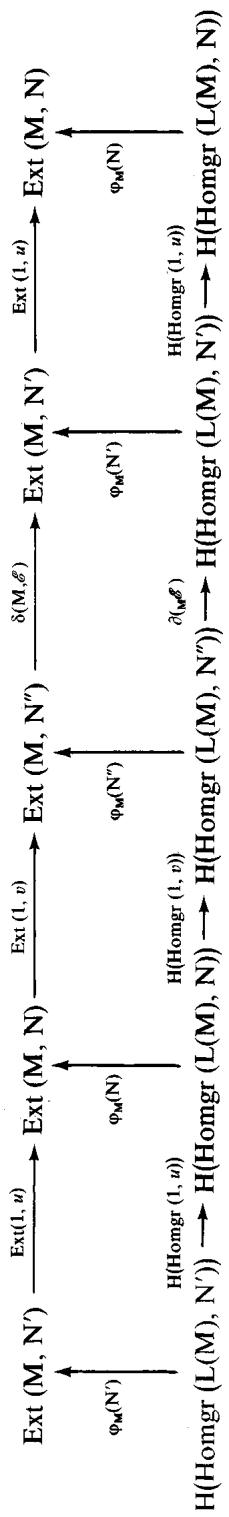
\includegraphics[keepaspectratio]{images/part001_97747f10.jpg}}

是 A-模的具有正合行的交换图。则 k-模的图

\[
\begin{array}{c} \operatorname{Ext} _ {\mathbf {A}} (\mathbf {M}, \mathbf {N} ^ {\prime \prime}) \xrightarrow {\delta (\mathbf {M} , \mathcal {E})} \operatorname{Ext} _ {\mathbf {A}} (\mathbf {M}, \mathbf {N} ^ {\prime}) \\ \operatorname{Ext} (f, g ^ {\prime \prime}) \Big | _ {\downarrow} \qquad \qquad \qquad \qquad \qquad \qquad \qquad \qquad \qquad \qquad \qquad \qquad \qquad \qquad \qquad \qquad \qquad \qquad \qquad \qquad \qquad \qquad \qquad \qquad \qquad \qquad \qquad \qquad \qquad \qquad \qquad \qquad \qquad \qquad \\ \operatorname{Ext} _ {\mathbf {A}} (\mathbf {M} _ {1}, \mathbf {N} _ {1} ^ {\prime \prime}) \xrightarrow {\delta (\mathbf {M} , \mathcal {E} _ {1})} \operatorname{Ext} _ {\mathbf {A}} (\mathbf {M} _ {1}, \mathbf {N} _ {1} ^ {\prime}) \end{array}
\]

是交换的。

这由 X，第 31 页，命题 2 应用于该交换图得出。

\[
\begin{array}{l} 0 \xrightarrow {\operatorname{Homgr} _ {A} (L (M) , N ^ {\prime})} \xrightarrow {\operatorname{Homgr} _ {A} (L (M) , N)} \xrightarrow {\operatorname{Homgr} _ {A} (L (M) , N ^ {\prime \prime})} 0 \\ \operatorname{Homgr} (L (f), g ^ {\prime}) \Big | _ {\downarrow} \quad \operatorname{Homgr} (1, u ^ {\prime}) \quad \Big | _ {\downarrow} \quad \operatorname{Homgr} (L (f), g) \quad \Big | _ {\downarrow} \quad \operatorname{Homgr} (L (f), g ^ {\prime \prime}) \\ 0 \xrightarrow {\operatorname{Homgr} _ {A} (L (M _ {1}) , N _ {1} ^ {\prime})} \xrightarrow {\operatorname{Homgr} _ {A} (L (M _ {1}) , N _ {1})} \xrightarrow {\operatorname{Homgr} _ {A} (L (M _ {1}) , N _ {1} ^ {\prime \prime})} 0 \end{array}
\]

设 N 是一个 A-模，且

\[
0 \rightarrow \mathbf {M} ^ {\prime} \xrightarrow {r} \mathbf {M} \xrightarrow {s} \mathbf {M} ^ {\prime \prime} \rightarrow 0\tag{$(\mathcal{F})$}
\]

一个 A-模的正合序列；复形序列

\[
\begin{array}{r l} (\mathcal {F} _ {\mathrm{N}}) & 0 \longrightarrow \operatorname{Homgr} _ {\mathrm{A}} (\mathrm{M} ^ {\prime \prime}, \mathrm{I} (\mathrm{N})) \xrightarrow {\operatorname{Homgr} (s , 1)} \operatorname{Homgr} _ {\mathrm{A}} (\mathrm{M}, \mathrm{I} (\mathrm{N})) \\ & \xrightarrow {\operatorname{Homgr} (r , 1)} \operatorname{Homgr} _ {\mathrm{A}} (\mathrm{M} ^ {\prime}, \mathrm{I} (\mathrm{N})) \longrightarrow 0 \end{array}
\]

是正合的（X，第 83 页，命题 2，a））；令

\[
\partial (\mathcal {F} _ {\mathrm{N}}): \mathrm{H} (\operatorname{Homgr} _ {\mathrm{A}} (\mathrm{M} ^ {\prime}, \mathrm{I} (\mathrm{N}))) \rightarrow \mathrm{H} (\operatorname{Homgr} _ {\mathrm{A}} (\mathrm{M} ^ {\prime \prime}, \mathrm{I} (\mathrm{N})))
\]

相应的连接同态。

定义3. --- 称相对于正合序列（\(\mathcal{F}\)）以及模 N 的扩张模的连接同态为复合同态

\[
\delta (\mathcal {F}, \mathrm{N}): \overline {{\varphi}} _ {\mathrm{N}} (\mathrm{M} ^ {\prime \prime}) \circ \partial (\mathcal {F} _ {\mathrm{N}}) \circ \overline {{\varphi}} _ {\mathrm{N}} (\mathrm{M} ^ {\prime}) ^ {- 1}: \operatorname{Ext} _ {\mathrm{A}} (\mathrm{M} ^ {\prime}, \mathrm{N}) \rightarrow \operatorname{Ext} _ {\mathrm{A}} (\mathrm{M} ^ {\prime \prime}, \mathrm{N}).
\]

这是一个 \(k\) -分次同态，其次数递增 1，其齐次分量记为 \(\delta^{n}(\mathcal{F}, \mathbf{N}) : \operatorname{Ext}_{\mathbf{A}}^{n}(\mathbf{M}', \mathbf{N}) \to \operatorname{Ext}_{\mathbf{A}}^{n+1}(\mathbf{M}'', \mathbf{N})\) .

然后我们如上证明以下命题：

定理2. —— k-模同态的右无界序列

\[
\begin{array}{r l} 0 & \xrightarrow {\quad} \operatorname{Hom} _ {A} (M ^ {\prime \prime}, N) \xrightarrow {\operatorname{Hom} (s , 1)} \operatorname{Hom} _ {A} (M, N) \xrightarrow {\operatorname{Hom} (r , 1)} \operatorname{Hom} _ {A} (M ^ {\prime}, N) \\ & \xrightarrow {\delta^ {\circ} (\mathcal {F} , N)} \operatorname{Ext} _ {A} ^ {1} (M ^ {\prime \prime}, N) \to \dots \xrightarrow {\delta^ {n - 1} (\mathcal {F} , N)} \operatorname{Ext} _ {A} ^ {n} (M ^ {\prime \prime}, N) \xrightarrow {\operatorname{Ext} ^ {n} (s , 1)} \operatorname{Ext} _ {A} ^ {n} (M, N) \\ & \xrightarrow {\operatorname{Ext} ^ {n} (r , 1)} \operatorname{Ext} _ {A} ^ {n} (M ^ {\prime}, N) \xrightarrow {\delta^ {n} (\mathcal {F} , N)} \operatorname{Ext} _ {A} ^ {n + 1} (M ^ {\prime \prime}, N) \to \dots \end{array}
\]

是正合的。

推论. —— 若 Ext \(_{A}^{1}\) (M'', N) = 0，序列

\[
0 \longrightarrow \operatorname{Hom} _ {\mathrm{A}} \left(\mathrm{M} ^ {\prime \prime}, \mathrm{N}\right) \xrightarrow {\operatorname{Hom} (s , 1)} \operatorname{Hom} _ {\mathrm{A}} (\mathrm{M}, \mathrm{N}) \xrightarrow {\operatorname{Hom} (r , 1)} \operatorname{Hom} _ {\mathrm{A}} \left(\mathrm{M} ^ {\prime}, \mathrm{N}\right) \longrightarrow 0
\]

是正合的。

命题 9. --- 设 \(g: \mathbf{N} \to \mathbf{N}_1\) 是 A-模的同态，且

\[
(\mathcal {F} _ {1})
\]

\[
0 \longrightarrow \mathbf {M} _ {1} ^ {\prime} \xrightarrow {r _ {1}} \mathbf {M} _ {1} \xrightarrow {s _ {1}} \mathbf {M} _ {1} ^ {\prime \prime} \longrightarrow 0
\]

\[
f ^ {\prime} \Big \downarrow \qquad f \Big \downarrow \qquad f ^ {\prime \prime} \Big \downarrow
\]

\[
0 \longrightarrow \mathbf {M} ^ {\prime} \stackrel {r} {\longrightarrow} \mathbf {M} \stackrel {s} {\longrightarrow} \mathbf {M} ^ {\prime \prime} \longrightarrow 0\tag{$(\mathcal{F})$}
\]

是 A-模的具有正合行的交换图。则 k-模的图

\[
\begin{array}{c} \operatorname{Ext} _ {\mathbf {A}} (\mathbf {M} ^ {\prime}, \mathbf {N}) \xrightarrow {\delta (\mathcal {F} , \mathbf {N})} \operatorname{Ext} _ {\mathbf {A}} (\mathbf {M} ^ {\prime \prime}, \mathbf {N}) \\ \operatorname{Ext} _ {\mathbf {A}} (f ^ {\prime}, g) \Big \downarrow \\ \operatorname{Ext} _ {\mathbf {A}} (\mathbf {M} _ {1} ^ {\prime}, \mathbf {N} _ {1}) \xrightarrow {\delta (\mathcal {F} _ {1} , \mathbf {N} _ {1})} \operatorname{Ext} _ {\mathbf {A}} (\mathbf {M} _ {1} ^ {\prime \prime}, \mathbf {N} _ {1}) \end{array}
\]

是交换的。

\subsection{投射模、内射模与扩张模}

命题10. —— 设 M 是一个 A-模。以下条件等价：

\begin{enumerate}
\def\labelenumi{(\roman{enumi})}
\item
  M 是投射的。
\item
  \(\operatorname{Ext}_{\mathbf{A}}^{i}(\mathbf{M},\mathbf{N}) = 0\) （对于每个 A-模 \(\mathbf{N}\) 以及每个整数 \(i > 0\)）.
\item
  \(\mathrm{Ext}_{\mathbf{A}}^{1}(\mathbf{M},\mathbf{N}) = 0\) （对于每个 A-模 \(\mathbf{N}\)）.
\item
  存在一个正合序列
\end{enumerate}

\[
0 \rightarrow \mathrm{K} \xrightarrow {u} \mathrm{P} \xrightarrow {r} \mathrm{M} \rightarrow 0,
\]

\(\text{其中 P 是投射的，且其中 } \text{ Ext}_{\mathbf{A}}^{1}(\mathbf{M}, \mathbf{K}) = 0.\)

\begin{enumerate}
\def\labelenumi{(\roman{enumi})}
\item
  \(\Rightarrow\) (ii)：这是 X 中命题 5 的推论，第 88 页。
\item
  \(\Rightarrow\) （iii）：这是平凡的。
\item
  \(\Rightarrow\) (iv)：这是显然的，因为 M 是自由模 P 的商模。
\item
  \(\Rightarrow\) (i)：由于 \(\operatorname{Ext}_{\mathbf{A}}^{1}(\mathbf{M},\mathbf{K}) = 0\) ，典范映射
\end{enumerate}

\[
\operatorname{Hom} _ {\mathbf {A}} (\mathbf {M}, \mathbf {P}) \rightarrow \operatorname{Hom} _ {\mathbf {A}} (\mathbf {M}, \mathbf {M})
\]

是满射（X，第 90 页，推论）；因此存在 v 的一个 A-线性截面，且 M 同构于 P 的一个直和项，从而是投射的。

命题11. --- 设 N 为一个 A-模。以下条件等价：

\begin{enumerate}
\def\labelenumi{(\roman{enumi})}
\item
  N 是内射的。
\item
  \(\operatorname{Ext}_{\mathbf{A}}^{i}(\mathbf{M},\mathbf{N}) = 0\) （对于每个 A-模 M 和每个整数 \(i > 0\)）.
\item
  \(\operatorname{Ext}_{\mathbf{A}}^{1}(\mathbf{M},\mathbf{N}) = 0\) （对于每个 A-模 \(\mathbf{M}\)）.
\item
  存在一个正合序列
\end{enumerate}

\[
0 \rightarrow \mathrm{N} \xrightarrow {u} \mathrm{I} \xrightarrow {v} \mathrm{C} \rightarrow 0,
\]

\(\text{其中 I 是内射的且其中 } \text{ Ext}_{\mathbf{A}}^{1} (\mathbf{C}, \mathbf{N}) = 0;\)

\begin{enumerate}
\def\labelenumi{(\alph{enumi})}
\setcounter{enumi}{21}
\item
  \(\operatorname{Ext}_{\mathbf{A}}^{1}(\mathbf{M},\mathbf{N}) = 0\) （对于每个单演 A-模 \(\mathbf{M}\)）.
\item
  \(\Rightarrow\) (ii)：这是 X 中命题 5 的推论，第 88 页。
\end{enumerate}

\begin{enumerate}
\def\labelenumi{(\roman{enumi})}
\setcounter{enumi}{1}
\item
  \(\Rightarrow\) (iii) \(\Rightarrow\) (v)：这是平凡的。
\item
  \(\Rightarrow\) (iv)：这是显然的，因为 N 是内射模的子模（X，第 19 页，推论 3）。
\item
  \(\Rightarrow\) (i)：由于 \(\operatorname{Ext}_{\mathbf{A}}^{1}(\mathbf{C},\mathbf{N}) = 0\) ，典范同态
\end{enumerate}

\[
\operatorname{Hom} _ {\mathbf {A}} (\mathrm{I}, \mathbf {N}) \rightarrow \operatorname{Hom} _ {\mathbf {A}} (\mathbf {N}, \mathbf {N})
\]

是满射的（X，第 93 页，推论）；因此存在 u 的一个 A-线性收缩，且 N 同构于 I 的一个直和项，从而 N 是内射的（X，第 16 页，命题 9）。

\begin{enumerate}
\def\labelenumi{(\alph{enumi})}
\setcounter{enumi}{21}
\tightlist
\item
  \(\Rightarrow\) (i)：若 a 是 A 的一个理想，则有 \(\operatorname{Ext}_{\mathbf{A}}^{1}(\mathbf{A}/\mathfrak{a},\mathbf{N})=0\) ；因此典范映射 \(\operatorname{Hom}_{\mathbf{A}}(\mathbf{A},\mathbf{N})\to\operatorname{Hom}_{\mathbf{A}}(\mathfrak{a},\mathbf{N})\) 是满射的，且 N 是内射的（X，第 16 页，命题 10）。
\end{enumerate}

\subsection{泛系数公式}

在本节中，我们考虑两个 A-模复形 (C, d) 和 (C', d')。考虑如下典范正合序列：

\[
0 \rightarrow \mathrm{Z} (\mathrm{C}) \stackrel {{j}} {{\rightarrow}} \mathrm{C} \stackrel {{\delta}} {{\rightarrow}} \mathrm{B} (\mathrm{C}) (- 1) \rightarrow 0,\tag{I}
\]

\((\mathrm{II}_{p})\)

\[
0 \to \mathrm{B} _ {p} (\mathrm{C}) \stackrel {{i}} {{\to}} \mathrm{Z} _ {p} (\mathrm{C}) \stackrel {{p}} {{\to}} \mathrm{H} _ {p} (\mathrm{C}) \to 0;
\]

我们从 δ 推出一个 k-同态

\[
\mathrm{H} (\text { Homgr } (\delta , 1)): \mathrm{H} (\text { Homgr } _ {\mathbf {A}} (\mathrm{B} (\mathbf {C}), \mathbf {C} ^ {\prime})) (1) \rightarrow \mathrm{H} (\text { Homgr } _ {\mathbf {A}} (\mathbf {C}, \mathbf {C} ^ {\prime}));
\]

由 \((\mathrm{II}_{p})\) 推出连接同态：

\[
\delta \left(\mathrm{II} _ {p}, \mathrm{H} ^ {q} \left(\mathrm{C} ^ {\prime}\right)\right): \operatorname{Hom} _ {\mathrm{A}} \left(\mathrm{B} _ {p} (\mathrm{C}), \mathrm{H} ^ {q} \left(\mathrm{C} ^ {\prime}\right)\right)\rightarrow \operatorname{Ext} _ {\mathrm{A}} ^ {1} \left(\mathrm{H} _ {p} (\mathrm{C}), \mathrm{H} ^ {q} \left(\mathrm{C} ^ {\prime}\right)\right).
\]

由此，通过过渡到乘积，得到 k-模的同态：

\[
\varphi^ {n}: \operatorname{Homgr} _ {\mathbf {A}} ^ {n} (\mathrm{B} (\mathrm{C}), \mathrm{H} (\mathrm{C} ^ {\prime})) \rightarrow \prod_ {p + q = n} \operatorname{Ext} _ {\mathbf {A}} ^ {1} \left(\mathrm{H} _ {p} (\mathrm{C}), \mathrm{H} ^ {q} (\mathrm{C} ^ {\prime})\right)
\]

还有典范同态（X，第 82 页）

\[
\lambda^ {n} (\mathrm{B} (\mathrm{C}), \mathrm{C} ^ {\prime}): \mathrm{H} ^ {n} \left(\operatorname{Homgr} _ {\mathrm{A}} (\mathrm{B} (\mathrm{C}), \mathrm{C} ^ {\prime})\right)\rightarrow \operatorname{Homgr} _ {\mathrm{A}} ^ {n} (\mathrm{B} (\mathrm{C}), \mathrm{H} (\mathrm{C} ^ {\prime})) .
\]

在这些记号下：

定理3. --- 假设 A-模 B(C) 和 Z(C) 是投射的。那么对每个 n，存在唯一的 k-模同态

\[
\beta^ {n}: \prod_ {p + q = n - 1} \operatorname{Ext} _ {\mathbf {A}} ^ {1} \left(\mathrm{H} _ {p} (\mathbf {C}), \mathrm{H} ^ {q} \left(\mathbf {C} ^ {\prime}\right)\right)\rightarrow \mathrm{H} ^ {n} \left(\operatorname{Homgr} _ {\mathbf {A}} \left(\mathrm{C}, \mathrm{C} ^ {\prime}\right)\right)
\]

从而使得图表交换

\[
\begin{array}{c} \operatorname{Homgr} _ {\mathbf {A}} ^ {n - 1} (\mathrm{B} (\mathrm{C}), \mathrm{H} (\mathrm{C} ^ {\prime})) \xleftarrow {\lambda^ {n - 1} (\mathrm{B} (\mathrm{C}) , \mathrm{C} ^ {\prime})} \mathrm{H} ^ {n - 1} (\operatorname{Homgr} _ {\mathbf {A}} (\mathrm{B} (\mathrm{C}), \mathrm{C} ^ {\prime})) \\ \prod_ {p + q = n - 1} \operatorname{Ext} _ {\mathbf {A}} ^ {1} (\mathrm{H} _ {p} (\mathrm{C}), \mathrm{H} ^ {q} (\dot {\mathrm{C}} ^ {\prime})) \xrightarrow {\beta^ {n}} \mathrm{H} ^ {n} (\operatorname{Homgr} _ {\mathbf {A}} (\mathrm{C}, \mathrm{C} ^ {\prime})). \end{array}
\]

分次 k-模的序列

\[
\begin{array}{r l} 0 \longrightarrow & \prod_ {p + q = n - 1} \operatorname{Ext} _ {\mathrm{A}} ^ {1} \left(\mathrm{H} _ {p} (\mathrm{C}), \mathrm{H} ^ {q} (\mathrm{C} ^ {\prime})\right) \xrightarrow {\beta^ {n}} \mathrm{H} ^ {n} \big (\mathrm{Homg} _ {\mathrm{A}} (\mathrm{C}, \mathrm{C} ^ {\prime}) \big) \\ & \xrightarrow {\lambda^ {n} (\mathrm{C} , \mathrm{C} ^ {\prime})} \prod_ {p + q = n} \mathrm{Hom} _ {\mathrm{A}} \left(\mathrm{H} _ {p} (\mathrm{C}), \mathrm{H} ^ {q} (\mathrm{C} ^ {\prime})\right) \to 0 \end{array}\tag{11}
\]

是正合的。

注记. --- 可以证明一个类似的命题，假设 \(\mathbf{B}_{n}(\mathbf{C}')\) 和 \(\mathbf{C}'/\mathbf{B}_{n}(\mathbf{C}')\) 对每个 n 都是内射的。

为简单起见，设 \(\mathbf{B} = \mathbf{B}(\mathbf{C}), \mathbf{Z} = \mathbf{Z}(\mathbf{C}), \mathbf{H} = \mathbf{H}(\mathbf{C})\) 和 \(\mathbf{H}' = \mathbf{H}(\mathbf{C}')\) 。由于 B 是投射的，由 (I) 可导出一个正合序列

\[
\begin{array}{r l}(1 2) \quad&0 \rightarrow \operatorname{Homgr} _ {\mathbf {A}} (\mathrm{B}, \mathrm{C} ^ {\prime}) (1) \xrightarrow {\operatorname{Homgr} (\delta , 1)} \operatorname{Homgr} _ {\mathbf {A}} (\mathrm{C}, \mathrm{C} ^ {\prime})\\&\xrightarrow {\operatorname{Homgr} (j , 1)} \operatorname{Homgr} _ {\mathbf {A}} (\mathrm{Z}, \mathrm{C} ^ {\prime}) \rightarrow 0.\end{array}
\]

引理2. --- 连接同态

\[
\mathrm{H} ^ {n} \left(\operatorname{Homgr} _ {\mathbf {A}} \left(\mathrm{Z}, \mathrm{C} ^ {\prime}\right)\right)\rightarrow \mathrm{H} ^ {n} \left(\operatorname{Homgr} _ {\mathbf {A}} \left(\mathrm{B}, \mathrm{C} ^ {\prime}\right)\right)
\]

与 (12) 相关联的连接同态等于 \((-1)^{n+1}\) H(Homgr(i, 1)).

事实上，设 \(a \in \mathbf{Z}^n(\text{Homgr}_A(Z, C'))\) ；这是一个次数递增 \(n\) 的、从 \(Z\) 到 \(C'\) 的复形态射，其值因此位于 \(Z(C')\) 中。由于正合序列 (I) 是分裂的（因为 B 是投射的）， \(a\) 延拓为一个元素 \(b\) ，它属于 \(\text{Homgr}_A^n(C, Z(C'))\) 。根据定义， \(a\) 的类在该连接同态下的像是 \(H^n(\text{Homgr}_A(B, C'))\) 中同态 \(u\) （从 \(B(C)\) 到 \(C'\) ）的类，使得对于 \(x \in C\) ，有

\[
u (d x) = \mathrm{D} b (x) = d ^ {\prime} b (x) - (- 1) ^ {n} b (d x) = (- 1) ^ {n + 1} b (d x) = (- 1) ^ {n + 1} a (d x),
\]

由此得出断言。

因此，与（12）相关联的同调正合列给出如下正合序列

\[
\rightarrow \mathrm{H} ^ {n} (\operatorname{Homgr} _ {\mathrm{A}} (Z, C ^ {\prime})) \xrightarrow {\mathrm{H} (\operatorname{Homgr} (i , 1))} \mathrm{H} ^ {n} (\operatorname{Homgr} _ {\mathrm{A}} (B, C ^ {\prime}))
\]

\[
\xrightarrow {\mathrm{H} (\text { Homgr } (\delta , 1))} \mathrm{H} ^ {n + 1} \left(\text { Homgr } _ {\mathrm{A}} \left(\mathrm{C}, \mathrm{C} ^ {\prime}\right)\right) \xrightarrow {\mathrm{H} (\text { Homgr } (j , 1))} \mathrm{H} ^ {n + 1} \left(\text { Homgr } _ {\mathrm{A}} \left(\mathrm{Z}, \mathrm{C} ^ {\prime}\right)\right)\rightarrow \dots .
\]

此外，由于 Z 是投射的，由 \((II_{p})\) 可导出正合序列

\[
0 \to \mathrm{Hom} _ {\mathbf {A}} (\mathrm{H} _ {p}, \mathrm{H} ^ {\prime q}) \to \mathrm{Hom} _ {\mathbf {A}} (Z _ {p}, \mathrm{H} ^ {\prime q}) \to \mathrm{Hom} _ {\mathbf {A}} (\mathrm{B} _ {p}, \mathrm{H} ^ {\prime q}) \to \mathrm{Ext} _ {\mathbf {A}} ^ {1} (\mathrm{H} _ {p}, \mathrm{H} ^ {\prime q}) \to 0,
\]

由此，通过取乘积，得到正合序列

\[
\begin{array}{r l} 0 \to \operatorname{Homgr} _ {\mathbf {A}} ^ {n} (\mathbf {H}, \mathbf {H} ^ {\prime}) & \to \operatorname{Homgr} _ {\mathbf {A}} ^ {n} (Z, \mathbf {H} ^ {\prime}) \to \operatorname{Homgr} _ {\mathbf {A}} ^ {n} (\mathbf {B}, \mathbf {H} ^ {\prime}) \\ & \to \prod_ {p + q = n} \operatorname{Ext} _ {\mathbf {A}} ^ {1} (\mathbf {H} _ {p}, \mathbf {H} ^ {\prime q}) \to 0. \end{array}
\]

最后，有第 1 号中的典范同态：

\[
\begin{array}{l} \lambda_ {\mathrm{B}} = \lambda (\mathrm{B}, \mathrm{C} ^ {\prime}): \mathrm{H} (\mathrm{Homgr} _ {\mathrm{A}} (\mathrm{B}, \mathrm{C} ^ {\prime})) \to \mathrm{Homgr} _ {\mathrm{A}} (\mathrm{B}, \mathrm{H} ^ {\prime}), \\ \lambda_ {\mathrm{Z}} = \lambda (\mathrm{Z}, \mathrm{C} ^ {\prime}): \mathrm{H} (\mathrm{Homgr} _ {\mathrm{A}} (\mathrm{Z}, \mathrm{C} ^ {\prime})) \to \mathrm{Homgr} _ {\mathrm{A}} (\mathrm{Z}, \mathrm{H} ^ {\prime}), \\ \lambda_ {\mathrm{C}} = \lambda (\mathrm{C}, \mathrm{C} ^ {\prime}): \mathrm{H} (\mathrm{Homgr} _ {\mathrm{A}} (\mathrm{C}, \mathrm{C} ^ {\prime})) \to \mathrm{Homgr} _ {\mathrm{A}} (\mathrm{H}, \mathrm{H} ^ {\prime}), \end{array}
\]

由此得到 X 第 97 页上的行正合图表。

该图表由 \(\lambda\) 同态的构造是交换的。此外，由于复形 B 和 Z 是分裂且投射的， \(\lambda_{\mathrm{B}}\) 和 \(\lambda_{\mathrm{Z}}\) 是双射的（X，第 84 页，推论 1）。由此一方面可推出， \(\lambda_{\mathrm{C}}^{n}\) 是满射的，其核等于 Im H \(^{n}\) (Homgr ( \(\delta\) , 1))，另一方面可推出， \(\varphi^{n-1} \circ \lambda_{\mathrm{B}}^{n-1}\) 是满射的，其核等于 Ker H \(^{n}\) (Homgr ( \(\delta\) , 1))。定理由此立即得出。

推论 1. --- 假设 B(C) 和 Z(C) 是投射的，且 B \(^{n}\) (C') 对每个 n 都是内射的。则正合序列 (11) 是分裂的。

这由定理及以下引理得出：

引理 3. --- 若 B(C) 是投射的且 \(\mathbf{B}_{n}(\mathbf{C}^{\prime})\) 对每个 \(n\) ，典范同态 \(\lambda(\mathbf{C}, \mathbf{C}^{\prime}): \mathrm{H}(\mathrm{Homgr}_{\mathbf{A}}(\mathbf{C}, \mathbf{C}^{\prime})) \to \mathrm{Homgr}_{\mathbf{A}}(\mathrm{H}(\mathbf{C}), \mathrm{H}(\mathbf{C}^{\prime}))\) 有一个 \(k\) -线性截面。

事实上，根据 X，第 35 页，注记 a) 和 b)，存在拟同构

\[
\varphi : \mathrm{C} \rightarrow \mathrm{H} (\mathrm{C}) \quad \text { and } \quad \varphi^ {\prime}: \mathrm{H} (\mathrm{C} ^ {\prime}) \rightarrow \mathrm{C} ^ {\prime}
\]

使得 \(\mathbf{H}(\varphi) = 1_{\mathbf{H}(\mathbf{C})}\) 和 \(\bar{\mathbf{H}} (\varphi^{\prime}) = 1_{\mathbf{H}(\mathbf{C}^{\prime})}\) .

在交换图中

\[
\begin{array}{l} \mathrm{H} (\operatorname{Homgr} _ {\mathbf {A}} (\mathrm{H} (\mathrm{C}), \mathrm{H} (\mathrm{C} ^ {\prime})) \xrightarrow {\mathrm{H} (\operatorname{Homgr} (\varphi , \varphi^ {\prime}))} \mathrm{H} (\operatorname{Homgr} _ {\mathbf {A}} (\mathrm{C}, \mathrm{C} ^ {\prime})) \\ \lambda (\mathrm{H} (\mathrm{C}), \mathrm{H} (\mathrm{C} ^ {\prime})) \Big | _ {\downarrow} \\ \operatorname{Homgr} _ {\mathbf {A}} (\mathrm{H} (\mathrm{C}), \mathrm{H} (\mathrm{C} ^ {\prime})) \xrightarrow {\operatorname{Homgr} (\mathrm{H} (\varphi) , \mathrm{H} (\varphi^ {\prime}))} \operatorname{Homgr} _ {\mathbf {A}} (\mathrm{H} (\mathrm{C}), \mathrm{H} (\mathrm{C} ^ {\prime}))  , \end{array}
\]

\(\lambda(H(C), H(C'))\) 是双射且 Homgr \((H(\varphi), H(\varphi'))\) 是恒等映射，由此得出断言。

Homgr \(^{n-1}\) (Z, H') → Homgr \(^{n-1}\) (B, H') → Φ \(^{n-1}\) → Πp+q=n-1 Ext \(^{1}\) (Hp, H'q) → 0

H \(^{n-1}\) (Homgr(A, C')) → H \(^{n-1}\) (Homgr(A, B, C')) → H \(^{n}\) (Homgr(A, C)) → H \(^{n}\) (Homgr(A, C)) → H \(^{n}\) (Homgr(A, B, C))

0 → Homgr \(^{n}\) (H, H') → Homgr \(^{n}\) (Z, H') → Homgr \(^{n}\) (B, H')

推论 2. --- 若 B(C) 和 Z(C) 是投射的，则对每个 A-模 N 和每个整数 n，存在一个分裂的正合序列：

\[
(1 3) \quad 0 \longrightarrow \operatorname{Ext} _ {\mathbf {A}} ^ {1} \left(\mathrm{H} _ {n - 1} (\mathrm{C}), \mathrm{N}\right) \xrightarrow {\beta^ {n}} \mathrm{H} ^ {n} \left(\operatorname{Homgr} _ {\mathbf {A}} (\mathrm{C}, \mathrm{N})\right) \xrightarrow {\lambda^ {n}} \operatorname{Hom} _ {\mathbf {A}} \left(\mathrm{H} _ {n} (\mathrm{C}), \mathrm{N}\right) \longrightarrow 0.
\]

推论 3（“泛系数公式”）. --- 设 A 是主理想环且 C 是自由的。则对每个 A-模 N 和每个整数 n，存在一个分裂的正合序列 (13)。

事实上，B(C) 和 Z(C) 作为自由模 C 的子模是自由的（VII，§ 3，定理 1 的推论 2）。

推论 4. --- 若 C 右有界且 C 和 H(C) 是投射的，则

\[
\lambda (C, C ^ {\prime}): H \left(\operatorname{Homgr} _ {A} (C, C ^ {\prime})\right)\rightarrow \operatorname{Homgr} _ {A} \left(H (C), H \left(C ^ {\prime}\right)\right)
\]

是双射。

由定理可知，只需证明 B(C) 和 Z(C) 是投射的。现在我们有正合序列

\[
\begin{array}{l} 0 \to \mathrm{B} _ {n} (\mathrm{C}) \to Z _ {n} (\mathrm{C}) \to \mathrm{H} _ {n} (\mathrm{C}) \to 0 \\ 0 \to Z _ {n} (\mathrm{C}) \to \mathrm{C} _ {n} \to \mathrm{B} _ {n - 1} (\mathrm{C}) \to 0, \end{array}
\]

因此 \((\mathbf{B}_{n - 1}(\mathbf{C})\) 是投射的) \(\Rightarrow (\mathbf{Z}_n(\mathbf{C})\) 是投射的) \(\Rightarrow (\mathbf{B}_n(\mathbf{C})\) 是投射的)。我们通过指出 \(\mathbf{B}_n(\mathbf{C}) = 0\) （对足够小的 \(n\) ）来结束。

\subsection{推广到多模复形；典范同构}

设 B, B' 为两个环，C 为 (A, B)-双模复形，C' 为 (A, B')-双模复形；则 (Homgr\_A (C, C′), D) 是 (B, B′)-双模复形，且典范同态 \(\lambda: H(\text{Homgr}_A (\text{C}, \text{C'})) \to \text{Homgr}_A (\text{H}(\text{C}), \text{H}(\text{C'}))\) 是 (B, B')-双模同态。

若 M 是 (A, B)-双模，N 是 (A, B')-双模，则 Homgr \(_{A}\) (L(M), I(N)) 是 (B, B')-双模复形，因此 Ext \(_{A}\) (M, N) 具有自然的分次 (B, B')-双模结构；在次数 0 项上，该结构与 Hom \(_{A}\) (M, N) 的结构一致（II，第 35 页）。

若 \(\lambda\in\mathbf{B},\lambda^{\prime}\in\mathbf{B}^{\prime}\) 并且如果我们记 \(\lambda_{\mathrm{M}},\lambda_{\mathrm{N}}^{\prime},\lambda_{\mathrm{E}},\lambda_{\mathrm{E}}^{\prime}\) 为位似 \(x\mapsto x\lambda,y\mapsto y\lambda^{\prime},z\mapsto\lambda z,z\mapsto z\lambda^{\prime}\) ，它们分别是 M, N, Ext \(_{\mathrm{A}}\) (M, N), Ext \(_{\mathrm{A}}\) (M, N) 的，则我们有

\[
\lambda_ {\mathrm{E}} = \operatorname{Ext} _ {\mathbf {A}} \left(\lambda_ {\mathbf {M}}, 1\right), \quad \lambda_ {\mathrm{E}} ^ {\prime} = \operatorname{Ext} \left(1, \lambda_ {\mathbf {N}} ^ {\prime}\right),
\]

这给出了 Ext \(_{A}\) (M, N) 的双模结构的另一种描述。我们把第 4 号和第 6 号推广到多模复形的情形留给读者。

设 C, C′ 和 C′′ 是 A-模的复形。映射的复合定义了一个次数为零的分次同态：

\[
\operatorname{Homgr} _ {\mathbf {A}} \left(\mathrm{C} ^ {\prime}, \mathrm{C} ^ {\prime \prime}\right) \otimes_ {k} \operatorname{Homgr} _ {\mathbf {A}} \left(\mathrm{C}, \mathrm{C} ^ {\prime}\right)\rightarrow \operatorname{Homgr} _ {\mathbf {A}} \left(\mathrm{C}, \mathrm{C} ^ {\prime \prime}\right).\tag{14}
\]

设 B、B'、E 为环，C、C'、C'' 分别为 (B', A)-双模、(A, E)-双模、(B, E)-双模的复形。通过限制 II 第 73 页的典范同构，得到 (B, B')-双模的一个双射同态：

\[
\operatorname{Homgr} _ {E} \left(C \otimes_ {A} C ^ {\prime}, C ^ {\prime \prime}\right)\rightarrow \operatorname{Homgr} _ {A} \left(C, \operatorname{Homgr} _ {E} \left(C ^ {\prime}, C ^ {\prime \prime}\right)\right).\tag{15}
\]

最后，设 B 为一个环，C 为右 B-模的复形，C' 为右 A-模的复形，C'' 为 (B, A)-双模的复形。我们由典范同态（II，第 75 页）推出

\[
\mathrm{C} _ {p} \otimes_ {\mathrm{B}} \operatorname{Hom} _ {\mathrm{A}} \left(\mathrm{C} _ {q} ^ {\prime}, \mathrm{C} _ {r} ^ {\prime \prime}\right)\rightarrow \operatorname{Hom} _ {\mathrm{A}} \left(\mathrm{C} _ {q} ^ {\prime}, \mathrm{C} _ {p} \otimes_ {\mathrm{B}} \mathrm{C} _ {r} ^ {\prime \prime}\right)
\]

一个次数为零的分次同态：

\[
\mathrm{C} \otimes_ {\mathrm{B}} \operatorname{Homgr} _ {\mathrm{A}} \left(\mathrm{C} ^ {\prime}, \mathrm{C} ^ {\prime \prime}\right)\rightarrow \operatorname{Homgr} _ {\mathrm{A}} \left(\mathrm{C} ^ {\prime}, \mathrm{C} \otimes_ {\mathrm{B}} \mathrm{C} ^ {\prime \prime}\right).\tag{16}
\]

当 C 是有限生成投射模时，此同态是双射的（II，第 75 页，命题 2）。

命题12.——同态（14）、（15）、（16）是复形的态射。

我们来证明它，例如对于同态（14）。记

\[
\kappa : \operatorname{Homgr} _ {\mathbf {A}} \left(\mathrm{C} ^ {\prime}, \mathrm{C} ^ {\prime \prime}\right) \otimes_ {k} \operatorname{Homgr} _ {\mathbf {A}} \left(\mathrm{C}, \mathrm{C} ^ {\prime}\right)\rightarrow \operatorname{Homgr} _ {\mathbf {A}} \left(\mathrm{C}, \mathrm{C} ^ {\prime \prime}\right)
\]

这个同态。设 \(f \in \operatorname{Homgr}_{\mathbf{A}}(\mathbf{C}', \mathbf{C}^{\prime})_{p}\) 和 \(g \in \operatorname{Homgr}_{\mathbf{A}}(\mathbf{C}, \mathbf{C}^{\prime})_{q}\) ；于是根据定义我们有 \(\kappa(f \otimes g) = f \circ g\) 。此外：

\[
\begin{array}{r l} \mathrm{D} (f \otimes g) = & \mathrm{D} f \otimes g + (- 1) ^ {p} f \otimes \mathrm{D} g = (d ^ {\prime \prime} \circ f) \otimes g - (- 1) ^ {p} (f \circ d ^ {\prime}) \otimes g + \\ & + (- 1) ^ {p} f \otimes (d ^ {\prime} \circ g) - (- 1) ^ {p + q} f \otimes (g \circ d), \end{array}
\]

由此可得

\[
\begin{array}{r l} & {\kappa \big (\mathbf {D} (f \otimes g) \big) = d ^ {\prime \prime} \circ f \circ g - (- 1) ^ {p} f \circ d ^ {\prime} \circ g +} \\ & {\qquad + (- 1) ^ {p} f \circ d ^ {\prime} \circ g - (- 1) ^ {p + q} f \circ g \circ d} \\ & {\qquad = d ^ {\prime \prime} \circ f \circ g - (- 1) ^ {p + q} f \circ g \circ d = \mathbf {D} (f \circ g) = \mathbf {D} \big (\kappa (f \otimes g) \big).} \end{array}
\]

类似地可证明同态(15)和(16)是复形的态射。

由态射 (14) 我们推出 \(k\) -模的同态（X，第 62 页）

\[
\mathrm{H} ^ {p} \left(\operatorname{Homgr} _ {\mathbf {A}} \left(\mathrm{C} ^ {\prime}, \mathrm{C} ^ {\prime \prime}\right)\right) \otimes_ {k} \mathrm{H} ^ {q} \left(\operatorname{Homgr} _ {\mathbf {A}} \left(\mathrm{C}, \mathrm{C} ^ {\prime}\right)\right)\rightarrow \mathrm{H} ^ {p + q} \left(\operatorname{Homgr} _ {\mathbf {A}} \left(\mathrm{C}, \mathrm{C} ^ {\prime \prime}\right)\right). \tag {17}
\]

取 C = A，我们看到同态：

\[
\operatorname{Homgr} _ {\mathbf {A}} \left(\mathrm{C} ^ {\prime}, \mathrm{C} ^ {\prime \prime}\right) \otimes_ {k} \mathrm{C} ^ {\prime} \rightarrow \mathrm{C} ^ {\prime \prime}\tag{18}
\]

它把 \(f \otimes x\) 映到 \(f(x)\) ，是左 A-模复形的一个态射；与之相伴的是分次 A-模的一个典范同态（X，第 80 页） \(\gamma : \mathrm{H}(\mathrm{Homgr}_{\mathbf{A}}(\mathbf{C}', \mathbf{C}')) \otimes_k \mathrm{H}(\mathbf{C}') \to \mathrm{H}(\mathbf{C}'')\) ，它对应于 \(k\) -模的典范同态

\[
\lambda : \mathrm{H} (\operatorname{Homgr} _ {\mathbf {A}} \left(\mathrm{C} ^ {\prime}, \mathrm{C} ^ {\prime \prime}\right)) \rightarrow \operatorname{Homgr} _ {\mathbf {A}} \left(\mathrm{H} (\mathrm{C} ^ {\prime}), \mathrm{H} (\mathrm{C} ^ {\prime \prime})\right).
\]

\section{非典范分解的使用}

我们沿用 § 4 的约定。
% semantic-fragments: legacy-input-seam
\relax{}
\subsection{\texorpdfstring{模的计算 \(\operatorname{Tor}^{\mathbf{A}}(\mathbf{P},\mathbf{M})\) 与 \(\operatorname{Ext}_{\mathbf{A}}(\mathbf{M},\mathbf{N})\)}{模的计算 \textbackslash operatorname\{Tor\}\^{}\{\textbackslash mathbf\{A\}\}(\textbackslash mathbf\{P\},\textbackslash mathbf\{M\}) 与 \textbackslash operatorname\{Ext\}\_\{\textbackslash mathbf\{A\}\}(\textbackslash mathbf\{M\},\textbackslash mathbf\{N\})}}

设 M、N 为左 A-模，P 为右 A-模。此外，设 \(a: R \rightarrow M\) 是 M 的一个左分解， \(b: S \rightarrow P\) 为 P 的一个左分解，且 \(c: N \rightarrow E\) 为 N 的一个右分解。

由 X，第 49 页，命题 3 及 3 bis，存在复形态射 \(\alpha: L(M) \to R\) , \(\beta: L(P) \to S\) , \(\gamma: E \to I(N)\) 使得 \(a \circ \alpha = p_{M}\) , \(b \circ \beta = p_{P}\) , \(\gamma \circ c = e_{N}\) ；且 \(\alpha\) , \(\beta\) , \(\gamma\) 的同伦类仅依赖于给定的分解。由 X，第 64 页，命题 3 及 X，第 84 页，命题 3，态射

\[
\beta \otimes \alpha : L (P) \otimes_ {A} L (M) \rightarrow S \otimes_ {A} R,
\]

\[
\operatorname{Homgr} _ {\mathbf {A}} (\alpha , \gamma): \operatorname{Homgr} _ {\mathbf {A}} (\mathrm{R}, \mathrm{E}) \rightarrow \operatorname{Homgr} _ {\mathbf {A}} (\mathrm{L} (\mathrm{M}), \mathrm{I} (\mathrm{N}))
\]

仅依赖于给定的分解，从而通过取同调，得到次数为 0 的分次 k-同态

\[
\psi (\mathrm{S}, \mathrm{R}): \operatorname{Tor} ^ {\mathrm{A}} (\mathrm{P}, \mathrm{M}) \rightarrow \mathrm{H} (\mathrm{S} \otimes_ {\mathrm{A}} \mathrm{R}),
\]

\[
\varphi (\mathrm{R}, \mathrm{E}): \mathrm{H} \left(\operatorname{Homgr} _ {\mathrm{A}} (\mathrm{R}, \mathrm{E})\right)\rightarrow \operatorname{Ext} _ {\mathrm{A}} (\mathrm{M}, \mathrm{N}),
\]

与 α、β、γ 的选择无关。

例如，取 \(a\) , \(b\) , \(c\) 分别为 M、P、N 的恒等映射，便得到同态 \(\psi(\mathbf{P}, \mathbf{M}) : \operatorname{Tor}^{\mathbf{A}}(\mathbf{P}, \mathbf{M}) \to \mathbf{P} \otimes_{\mathbf{A}} \mathbf{M}\) 与 \(\varphi(\mathbf{M}, \mathbf{N}) : \operatorname{Hom}_{\mathbf{A}}(\mathbf{M}, \mathbf{N}) \to \operatorname{Ext}_{\mathbf{A}}(\mathbf{M}, \mathbf{N})\) 在 X，第 68 页，注记 2）以及 X，第 87 页，注记 2）中引入。

定理 1. --- a) 若分解 R 或 S 中有一个是平坦的，则 \(\psi(S, R)\) 是 \(k\) -分次模的同构。

\begin{enumerate}
\def\labelenumi{\alph{enumi})}
\setcounter{enumi}{1}
\item
  若 R 是投射的，或 E 是内射的，则 \(\varphi(\mathbf{R},\mathbf{E})\) 是 \(k\) -分次模的同构。
\item
  例如假设 R 是平坦的，并如上选择 \(\alpha\) 与 \(\beta\) 。同态 \(\beta \otimes \alpha\) 是以下态射的复合
\end{enumerate}

\[
\mathrm{L} (\mathrm{P}) \otimes_ {\mathrm{A}} \mathrm{L} (\mathrm{M}) \xrightarrow {l _ {\mathrm{L} (\mathrm{P})} \otimes \alpha} \mathrm{L} (\mathrm{P}) \otimes_ {\mathrm{A}} \mathrm{R} \xrightarrow {\beta \otimes 1 _ {\mathrm{R}}} \mathrm{S} \otimes_ {\mathrm{A}} \mathrm{R}.
\]

由于 L(P)（相应地，R）是平坦的，且 \(\alpha\) （相应地， \(\beta\) ）是同调同构，故 \(1_{L(P)} \otimes \alpha\) （相应地， \(\beta \otimes 1_R\) ）也是同调同构（X，第 67 页，命题 4）。因此 \(\beta \otimes \alpha\) 是同调同构，且 \(\psi(S, R) = H(\beta \otimes \alpha)\) 是双射。

\begin{enumerate}
\def\labelenumi{\alph{enumi})}
\setcounter{enumi}{1}
\tightlist
\item
  类似地论证，使用 X，第 86 页，命题 4。
\end{enumerate}

推论. --- 若 R 是 M 的平坦分解，则同态

\[
\psi (\mathrm{P}, \mathrm{R}): \operatorname{Tor} ^ {\mathbf {A}} (\mathrm{P}, \mathrm{M}) \rightarrow \mathrm{H} (\mathrm{P} \otimes_ {\mathbf {A}} \mathrm{R})
\]

是双射。若 R 是 M 的投射分解，则同态

\[
\varphi (\mathrm{R}, \mathrm{N}): \mathrm{H} \left(\operatorname{Homgr} _ {\mathrm{A}} (\mathrm{R}, \mathrm{N})\right)\rightarrow \operatorname{Ext} _ {\mathrm{A}} (\mathrm{M}, \mathrm{N})
\]

是双射。若 E 是 N 的内射分解，则同态

\[
\varphi (\mathbf {M}, \mathbf {E}): \mathrm{H} \left(\operatorname{Homgr} _ {\mathbf {A}} (\mathbf {M}, \mathbf {E})\right)\rightarrow \operatorname{Ext} _ {\mathbf {A}} (\mathbf {M}, \mathbf {N})
\]

是双射。

注记. --- k-模的图表

\[
\begin{array}{c} \operatorname{Tor} ^ {\mathbf {A}} (\mathrm{P}, \mathrm{M}) \xrightarrow {\psi (\mathrm{S} , \mathrm{R})} \mathrm{H} (\mathrm{S} \otimes_ {\mathbf {A}} \mathrm{R}) \\ \sigma_ {\mathrm{P}, \mathrm{M}} \Biggl \downarrow \\ \operatorname{Tor} ^ {\mathbf {A} ^ {\circ}} (\mathrm{M} ^ {\circ}, \mathrm{P} ^ {\circ}) \xrightarrow {\psi (\mathrm{R} ^ {\circ} , \mathrm{S} ^ {\circ})} \mathrm{H} (\mathrm{R} ^ {\circ} \otimes_ {\mathbf {A} ^ {\circ}} \mathrm{S} ^ {\circ}), \end{array}
\]

其中 \(\sigma_{\mathrm{P,M}}\) 与 \(\sigma(\mathrm{S},\mathrm{R})\) 是交换同构（X，第 71 页和第 63 页），该图表是交换的：实际上，它是通过取同调，由复形的交换图

\[
\begin{array}{c c} \mathrm{L} (\mathrm{P}) \otimes_ {\mathrm{A}} \mathrm{L} (\mathrm{M}) & \xrightarrow {\beta \otimes \alpha} \mathrm{S} \otimes_ {\mathrm{A}} \mathrm{R} \\ \sigma (\mathrm{L} (\mathrm{P}), \mathrm{L} (\mathrm{M})) \Big \downarrow & \Big \downarrow \sigma (\mathrm{S}, \mathrm{R}) \\ \mathrm{L} (\mathrm{M} ^ {\circ}) \otimes_ {\mathrm{A} ^ {\circ}} \mathrm{L} (\mathrm{P} ^ {\circ}) & \xrightarrow {\alpha \otimes \beta} \mathrm{R} ^ {\circ} \otimes_ {\mathrm{A} ^ {\circ}} \mathrm{S} ^ {\circ} \end{array}
\]

（“态射 \(\psi\) 与交换同构相容”）。

类似地，设 \(a_{1}: \mathbb{R}_{1} \to \mathbb{M}\) , \(b_{1}: \mathbb{S}_{1} \to \mathbb{P}\) , \(c_{1}: \mathbb{N} \to \mathbb{E}_{1}\) 为复形态射，其中 \(\mathbb{R}_{1}\) 与 \(\mathbb{S}_{1}\) 是投射的且在右侧为零，并且 \(\mathbb{E}_{1}\) 是内射的且在左侧为零。根据 X，第 49 页，命题 3 和 3 bis，存在复形态射

\[
\alpha_ {1}: \mathrm{R} _ {1} \rightarrow \mathrm{L} (\mathrm{M}), \quad \beta_ {1}: \mathrm{S} _ {1} \rightarrow \mathrm{L} (\mathrm{P}), \quad \gamma_ {1}: \mathrm{I} (\mathrm{N}) \rightarrow \mathrm{E} _ {1}
\]

使得 \(p_{\mathrm{M}} \circ \alpha_{1} = a_{1}, p_{\mathrm{P}} \circ \beta_{1} = b_{1}, \gamma_{1} \circ e_{\mathrm{N}} = c_{1}\) 由此得到复形态射

\[
\beta_ {1} \otimes \alpha_ {1}: S _ {1} \otimes_ {A} R _ {1} \rightarrow L (P) \otimes_ {A} L (M),
\]

\[
\operatorname{Homgr} _ {\mathbf {A}} \left(\alpha_ {1}, \gamma_ {1}\right): \operatorname{Homgr} _ {\mathbf {A}} \left(\mathrm{L} (\mathrm{M}), \mathrm{I} (\mathrm{N})\right)\rightarrow \operatorname{Homgr} _ {\mathbf {A}} \left(\mathrm{R} _ {1}, \mathrm{E} _ {1}\right),
\]

并且通过取同调，得到次数为 0 的 k-线性分次映射：

\[
\begin{array}{l} \psi^ {\prime} (\mathbf {S} _ {1}, \mathbf {R} _ {1}): \mathrm{H} (\mathbf {S} _ {1} \otimes_ {\mathbf {A}} \mathbf {R} _ {1}) \to \operatorname{Tor} ^ {\mathbf {A}} (\mathbf {P}, \mathbf {M}) \\ \varphi^ {\prime} (\mathbf {R} _ {1}, \mathbf {E} _ {1}): \operatorname{Ext} _ {\mathbf {A}} (\mathbf {M}, \mathbf {N}) \to \mathrm{H} (\operatorname{Homgr} _ {\mathbf {A}} (\mathbf {R} _ {1}, \mathbf {E} _ {1})) \end{array}
\]

如上所述，可验证这些映射不依赖于 \(\alpha_{1}\) , \(\beta_{1}\) , \(\gamma_{1}\) 的选择。

命题 1. --- 若 \(a_{1}\) , \(b_{1}\) , \(c_{1}\) 是同调同构，则 \(\psi^{\prime}(\mathbf{S}_{1},\mathbf{R}_{1})\) 与 \(\varphi^{\prime}(\mathbf{R}_{1},\mathbf{E}_{1})\) 分别是双射 \(\psi(\mathbf{S}_{1},\mathbf{R}_{1})\) 与 \(\varphi(\mathbf{R}_{1},\mathbf{E}_{1})\) 的逆双射。事实上， \(f = (\beta \otimes \alpha) \circ (\beta_{1} \otimes \alpha_{1})\) 是复形 \(\mathbf{S}_{1} \otimes_{\mathbf{A}} \mathbf{R}_{1}\) 到自身的态射，且有 \((b_{1} \circ \alpha_{1}) \circ f = f\) 。根据 X，第 49 页，命题 3 和 3 bis， \(f\) 是同伦等价，因此 H(f) = 1 且

\[
\psi \left(\mathrm{S} _ {1}, \mathrm{R} _ {1}\right) \circ \psi^ {\prime} \left(\mathrm{S} _ {1}, \mathrm{R} _ {1}\right) = \mathrm{H} (\beta \otimes \alpha) \circ \mathrm{H} \left(\beta_ {1} \otimes \alpha_ {1}\right) = \mathrm{H} (f) = 1;
\]

同理 \(\psi'(S_1, R_1) \circ \psi(S_1, R_1) = 1\) 。对映射 \(\varphi\) 与 \(\varphi'\) 可类似论证。

例。--- 1) 设 \(a\) 是 A 的一个元素，使得映射 \(\varphi : x \mapsto xa\) 从 A 到自身是单射（ \(a\) 不是右零因子）。利用分解

\[
0 \rightarrow \mathrm{A} _ {s} \xrightarrow {\varphi} \mathrm{A} _ {s} \rightarrow \mathrm{A} / \mathrm{A} a \rightarrow 0
\]

我们看到，对于每个右 A-模 M，有

\[
\operatorname{Tor} _ {i} ^ {\mathbf {A}} (\mathbf {M}, \mathbf {A} / \mathbf {A} a) = 0 \quad \text { for } \quad i > 1
\]

并且该 \(k\) -模 \(\operatorname{Tor}_1^{\mathbf{A}}(\mathbf{M}, \mathbf{A} / \mathbf{A}a)\) 同构于 \(\operatorname{Ker}(a_{\mathbf{M}})\) .

类似地，对于每个左 A-模 M，有

\[
\operatorname{Ext} _ {\mathbf {A}} ^ {i} (\mathbf {A} / \mathbf {A} a, \mathbf {M}) = 0 \quad \text { for } \quad i > 1
\]

且 \(k\) -模 \(\operatorname{Ext}_{\mathbf{A}}^{1}(\mathbf{A}/\mathbf{A}a, \mathbf{M})\) 同构于 \(\mathbf{M}/a\mathbf{M}\) .

\begin{enumerate}
\def\labelenumi{\arabic{enumi})}
\setcounter{enumi}{1}
\tightlist
\item
  设 A 是一个整环；令 K 为 A 的分式域，M 为一个 A-模。利用平坦分解
\end{enumerate}

\[
0 \rightarrow \mathrm{A} \rightarrow \mathrm{K} \rightarrow \mathrm{K} / \mathrm{A} \rightarrow 0
\]

（X，第 9 页，例 5），我们看到 \(\operatorname{Tor}_{i}^{\mathbf{A}}(\mathbf{K}/\mathbf{A}, \mathbf{M}) = 0\) 对 \(i > 1\) 成立；此外，考虑到 II，第 116 页，命题 26, (ii)，A-模 \(\operatorname{Tor}_{1}^{\mathbf{A}}(\mathbf{K}/\mathbf{A}, \mathbf{M})\) 同构于 M 的挠子模。

\begin{enumerate}
\def\labelenumi{\arabic{enumi})}
\setcounter{enumi}{2}
\tightlist
\item
  设 A 是一个诺特局部环，用 m 表示其极大理想，并令 \(\kappa = \mathbf{A} / \mathfrak{m}\) 。设 M 为有限生成的 A-模，P 为 M 的一个极小投射分解（X，第 54 页）。对每个 \(n \geqslant 0\) ， \(\kappa\) -向量空间 \(\operatorname{Tor}_n^{\mathbf{A}}(\kappa, \mathbf{M})\) 与 \(\operatorname{Ext}_{\mathbf{A}}^{n}(\mathbf{M}, \kappa)\) 都是有限维的，其维数等于自由 A-模 \(\mathbf{P}_n\) 的秩；事实上，复形 \(\kappa \otimes_{\mathbf{A}} \mathbf{P}\) 与 \(\operatorname{Homgr}_{\mathbf{A}}(\mathbf{P}, \kappa)\) 的微分均为零。
\end{enumerate}

\subsection{\texorpdfstring{映射的计算 \(\operatorname{Tor}^{\mathbf{A}}(g, f)\) 与 \(\operatorname{Ext}_{\mathbf{A}}(f, h)\)}{映射的计算 \textbackslash operatorname\{Tor\}\^{}\{\textbackslash mathbf\{A\}\}(g, f) 与 \textbackslash operatorname\{Ext\}\_\{\textbackslash mathbf\{A\}\}(f, h)}}

设 \(f: \mathbf{M} \to \mathbf{M}'\) , \(h: \mathbf{N}' \to \mathbf{N}\) 分别为左 A-模的同态， \(g: \mathbf{P} \to \mathbf{P}'\) 为右 A-模的同态， \(a: \mathbf{R} \to \mathbf{M}\) , \(a': \mathbf{R}' \to \mathbf{M}'\) , \(b: \mathbf{S} \to \mathbf{P}\) , \(b': \mathbf{S}' \to \mathbf{P}'\) 分别为 M、M'、P、P' 的左分解， \(c: \mathbf{N} \to \mathbf{E}\) , \(c': \mathbf{N}' \to \mathbf{E}'\) 分别为 N 与 N' 的右分解， \(\tilde{f}: \mathbf{R} \to \mathbf{R}'\) , \(\tilde{g}: \mathbf{S} \to \mathbf{S}'\) , \(\tilde{h}: \mathbf{E}' \to \mathbf{E}\) 为复形态射，使得

\[
a ^ {\prime} \circ \tilde {f} = f \circ a, b ^ {\prime} \circ \tilde {g} = g \circ b, \tilde {h} \circ c ^ {\prime} = c \circ h.
\]

命题2. --- 以下两个图表是可交换的：

\[
\begin{array}{c} \operatorname{Tor} ^ {\mathbf {A}} (\mathrm{P}, \mathrm{M}) \xrightarrow {\psi (\mathrm{S} , \mathrm{R})} \mathrm{H} (\mathrm{S} \otimes_ {\mathbf {A}} \mathrm{R}) \\ \operatorname{Tor} ^ {\mathbf {A}} (g, f) \Big \downarrow \qquad \qquad \qquad \qquad \qquad \qquad \qquad \qquad \qquad \qquad \qquad \qquad \qquad \qquad \qquad \qquad \qquad \qquad \qquad \qquad \qquad \qquad \qquad \qquad \qquad \qquad \qquad \qquad \qquad \qquad \qquad \qquad \qquad \qquad \\ \operatorname{Tor} ^ {\mathbf {A}} (\mathrm{P} ^ {\prime}, \mathrm{M} ^ {\prime}) \xrightarrow {\psi (\mathrm{S} ^ {\prime} , \mathrm{R} ^ {\prime})} \mathrm{H} (\mathrm{S} ^ {\prime} \otimes_ {\mathbf {A}} \mathrm{R} ^ {\prime})  , \end{array}
\]

\[
\begin{array}{c} \mathrm{H} (\operatorname{Homgr} _ {\mathbf {A}} (\mathrm{R} ^ {\prime}, \mathrm{E} ^ {\prime})) \xrightarrow {\varphi (\mathrm{R} ^ {\prime} , \mathrm{E} ^ {\prime})} \operatorname{Ext} _ {\mathbf {A}} (\mathrm{M} ^ {\prime}, \mathrm{N} ^ {\prime}) \\ \mathrm{H} (\operatorname{Homgr} _ {\mathbf {A}} (\tilde {f}, \tilde {h})) \Biggl \downarrow \\ \mathrm{H} (\operatorname{Homgr} _ {\mathbf {A}} (\mathrm{R}, \mathrm{E})) \xrightarrow {\varphi (\mathrm{R} , \mathrm{E})} \operatorname{Ext} _ {\mathbf {A}} (\mathrm{M}, \mathrm{N}). \end{array}
\]

设 \(\alpha: L(M) \to R\) , \(\alpha': L(M') \to R'\) , \(\gamma: L(P) \to S\) , \(\gamma': L(P') \to S'\) 为复形态射，使得

\[
a \circ \alpha = p _ {\mathrm{M}}, a ^ {\prime} \circ \alpha^ {\prime} = p _ {\mathrm {M^ {\prime}}}, b \circ \gamma = p _ {\mathrm{P}}, b ^ {\prime} \circ \gamma^ {\prime} = p _ {\mathrm {P^ {\prime}}}.
\]

根据定义， \(\mathrm{H}(\tilde{g}\otimes\tilde{f})\circ\psi(\mathrm{S},\mathrm{R})\) 等于

\[
\mathrm{H} (\tilde {g} \otimes \tilde {f}) \circ \mathrm{H} (\gamma \otimes \alpha) = \mathrm{H} ((\tilde {g} \circ \gamma) \otimes (\tilde {f} \circ \alpha)),
\]

而 \(\psi(\mathbf{S}',\mathbf{R}')\circ\mathrm{Tor}^{\mathbf{A}}(g,f)\) 等于

\[
\mathrm{H} \left(\gamma^ {\prime} \otimes \alpha^ {\prime}\right) \circ \mathrm{H} \left(\mathrm{L} (g) \otimes \mathrm{L} (f)\right) = \mathrm{H} \left(\left(\gamma^ {\prime} \circ \mathrm{L} (g)\right) \otimes \left(\alpha^ {\prime} \circ \mathrm{L} (f)\right)\right).
\]

另一方面， \(\alpha' \circ L(f)\) 与 \(\tilde{f} \circ \alpha\) 是从 L(M) 到 R′ 的两个态射，使得 \(a' \circ (\alpha' \circ L(f)) = p_{\mathrm{M}} \circ L(f) = f \circ p_{\mathrm{M}} = f \circ a \circ \alpha = a' \circ (\tilde{f} \circ \alpha)\) 。根据 X，第 49 页，命题 3， \(\alpha' \circ L(f)\) 与 \(\tilde{f} \circ \alpha\) 是同伦的；同样地 \(\gamma' \circ L(g)\) 与 \(\tilde{g} \circ \gamma\) 是同伦的，因此 \((\gamma' \circ L(g)) \otimes (\alpha' \circ L(f))\) 与 \((\tilde{g} \circ \gamma) \otimes (\tilde{f} \circ \alpha)\) 根据 X，第 64 页，命题 3 也是同伦的。因此我们有

\[
\begin{array}{r l} \mathrm{H} (\tilde {g} \otimes \tilde {f}) \circ \psi (\mathrm{S}, \mathrm{R}) & = \mathrm{H} ((\tilde {g} \circ \gamma) \otimes (\tilde {f} \circ \alpha)) = \mathrm{H} ((\gamma^ {\prime} \circ \mathrm{L} (g)) \otimes (\alpha^ {\prime} \circ \mathrm{L} (f))) \\ & = \psi (\mathrm{S} ^ {\prime}, \mathrm{R} ^ {\prime}) \circ \mathrm{Tor} ^ {\mathrm{A}} (g, f). \end{array}
\]

我们类似地论证第二个图表。

注记. --- 类似地考虑复形态射的交换图表。

\[
\begin{array}{c c c} \mathrm{R} _ {1} \xrightarrow {a _ {1}} \mathrm{M} & \mathrm{S} _ {1} \xrightarrow {b _ {1}} \mathrm{P} & \mathrm{N} ^ {\prime} \xrightarrow {c _ {1} ^ {\prime}} \mathrm{E} ^ {\prime} \\ \tilde {f} \Big \downarrow & f \Big \downarrow & g \Big \downarrow \\ \mathrm{R} _ {1} ^ {\prime} \xrightarrow {a _ {1} ^ {\prime}} \mathrm{M} ^ {\prime} & \mathrm{S} _ {1} ^ {\prime} \xrightarrow {b _ {1} ^ {\prime}} \mathrm{P} ^ {\prime} & \mathrm{N} \xrightarrow {c _ {1}} \mathrm{E} _ {1} \end{array}
\]

其中复形 \(R_{1}\) , \(R_{1}^{\prime}\) , \(S_{1}\) , \(S_{1}^{\prime}\) 是投射的且在右侧为零，而复形 \(E_{1}\) , \(E_{1}^{\prime}\) 是内射的且在左侧为零。那么

\[
\begin{array}{r l} & {\mathrm{Tor} ^ {\mathbf {A}} (g, f) \circ \psi^ {\prime} (\mathrm{S} _ {1}, \mathrm{R} _ {1}) = \psi^ {\prime} (\mathrm{S} _ {1} ^ {\prime}, \mathrm{R} _ {1} ^ {\prime}) \circ \mathrm{H} (\tilde {g} \otimes \tilde {f})} \\ & {\varphi^ {\prime} (\mathrm{R} _ {1}, \mathrm{E} _ {1}) \circ \mathrm{Ext} _ {\mathbf {A}} (f, h) = \mathrm{H} (\mathrm{Homgr} _ {\mathbf {A}} (\tilde {f}, \tilde {h})) \circ \varphi^ {\prime} (\mathrm{R} _ {1} ^ {\prime}, \mathrm{E} _ {1} ^ {\prime})} \end{array}
\]

这由与命题 2 类似的论证得到。

\subsection{连接同态的计算}

考虑一个交换图

\begin{enumerate}
\def\labelenumi{(\arabic{enumi})}
\tightlist
\item
\end{enumerate}

\[
\begin{array}{c} 0 \longrightarrow \mathrm{R} ^ {\prime} \xrightarrow {\tilde {u}} \mathrm{R} \xrightarrow {\tilde {v}} \mathrm{R} ^ {\prime \prime} \longrightarrow 0 \\ a ^ {\prime} \Big \downarrow \qquad \qquad \qquad \qquad \qquad \qquad \qquad \qquad \qquad \qquad \qquad \qquad \qquad \qquad \qquad \qquad \qquad \qquad \qquad \qquad \qquad \qquad \qquad \qquad \qquad \qquad \qquad \qquad \qquad \qquad \qquad \qquad \qquad \qquad \\ 0 \longrightarrow \mathrm{M} ^ {\prime} \xrightarrow {u} \mathrm{M} \xrightarrow {v} \mathrm{M} ^ {\prime \prime} \longrightarrow 0 \end{array}\tag{2}
\]

其中第一行 (1) 是左 A-模复形的正合列，第二行 (2) 是左 A-模的正合列，且竖直箭头为左分解。

命题 3. --- a) 设 P 是一个 A-模， \(b: S \to P\) 为 P 的一个左分解；假设 k-模复形序列

\[
0 \rightarrow \mathrm{S} \otimes_ {\mathrm{A}} \mathrm{R} ^ {\prime} \xrightarrow {l _ {\mathrm{s}} \otimes \tilde {u}} \mathrm{S} \otimes_ {\mathrm{A}} \mathrm{R} \xrightarrow {l _ {\mathrm{s}} \otimes \tilde {v}} \mathrm{S} \otimes_ {\mathrm{A}} \mathrm{R} ^ {\prime \prime} \rightarrow 0\tag{3}
\]

是正合的。则下面的图表是交换的：

\[
\begin{array}{c c c} \operatorname{Tor} ^ {\mathbf {A}} (\mathrm{P}, \mathrm{M} ^ {\prime \prime}) & \xrightarrow {\partial (\mathrm{P} , (2))} & \operatorname{Tor} ^ {\mathbf {A}} (\mathrm{P}, \mathrm{M} ^ {\prime}) \\ \psi (\mathrm{S}, \mathrm{R} ^ {\prime \prime}) \Big \downarrow & & \Big \downarrow \psi (\mathrm{S}, \mathrm{R} ^ {\prime}) \\ \mathrm{H} (\mathrm{S} \otimes_ {\mathbf {A}} \mathrm{R} ^ {\prime \prime}) & \xrightarrow {\partial ((3))} & \mathrm{H} (\mathrm{S} \otimes_ {\mathbf {A}} \mathrm{R} ^ {\prime}). \end{array}
\]

\begin{enumerate}
\def\labelenumi{\alph{enumi})}
\setcounter{enumi}{1}
\tightlist
\item
  设 N 是一个左 A-模， \(c : N \to E\) 为 N 的一个右分解；假设 k-模复形序列
\end{enumerate}

\begin{enumerate}
\def\labelenumi{(\arabic{enumi})}
\setcounter{enumi}{3}
\tightlist
\item
\end{enumerate}

\(0 \to \text{Homgr}_{\mathbf{A}}(\mathbf{R}^{\prime \prime}, \mathbf{E}) \xrightarrow{\text{Homgr}_{\mathbf{A}}(\tilde{\imath}, 1)} \text{Homgr}_{\mathbf{A}}(\mathbf{R}, \mathbf{E}) \xrightarrow{\text{Homgr}_{\mathbf{A}}(\tilde{\mu}, 1)} \text{Homgr}_{\mathbf{A}}(\mathbf{R}^{\prime}, \mathbf{E}) \to 0\) 是正合的。则下面的图表是交换的：

\[
\begin{array}{c} \mathrm{H} (\operatorname{Homgr} _ {\mathbf {A}} (\mathrm{R} ^ {\prime}, \mathrm{E})) \xrightarrow {\delta ((4))} \mathrm{H} (\operatorname{Homgr} _ {\mathbf {A}} (\mathrm{R} ^ {\prime \prime}, \mathrm{E})) \\ \varphi (\mathrm{R} ^ {\prime}, \mathrm{E}) \Big \downarrow \\ \operatorname{Ext} _ {\mathbf {A}} (\mathrm{M} ^ {\prime}, \mathrm{N}) \xrightarrow {\partial ((2) , \mathrm{N})} \operatorname{Ext} _ {\mathbf {A}} (\mathrm{M} ^ {\prime \prime}, \mathrm{N}). \end{array}
\]

例如证明 \(a\) )。设 \(\beta: L(P) \to S\) 是复形的态射，使得 \(b \circ \beta = p_{P}\) ；考虑 \(k\) -复形的图表

\[
\begin{array}{c}0 \rightarrow \mathrm{S} \otimes_ {\mathrm{A}} \mathrm{R} ^ {\prime} \xrightarrow {1 \otimes \tilde {u}} \mathrm{S} \otimes_ {\mathrm{A}} \mathrm{R} \xrightarrow {1 \otimes \tilde {v}} \mathrm{S} \otimes_ {\mathrm{A}} \mathrm{R} ^ {\prime \prime} \longrightarrow 0\\\beta \otimes 1 _ {\mathrm{R}} \Bigg | \quad \beta \otimes 1 _ {\mathrm{R}} \Bigg | \quad \beta \otimes 1 _ {\mathrm{R}} \Bigg |\\0 \rightarrow \mathrm{L(P)} \otimes_ {\mathrm{A}} \mathrm{R} ^ {\prime} \xrightarrow {1 \otimes \tilde {u}} \mathrm{L(P)} \otimes_ {\mathrm{A}} \mathrm{R} \xrightarrow {1 \otimes \tilde {v}} \mathrm{L(P)} \otimes_ {\mathrm{A}} \mathrm{R} ^ {\prime \prime} \longrightarrow 0\\1 \otimes a ^ {\prime} \Bigg | \quad 1 \otimes a \Bigg | \quad 1 \otimes a ^ {\prime \prime} \Bigg |\\0 \rightarrow \mathrm{L(P)} \otimes_ {\mathrm{A}} \mathrm{M} ^ {\prime} \xrightarrow {1 \otimes u} \mathrm{L(P)} \otimes_ {\mathrm{A}} \mathrm{M} \xrightarrow {1 \otimes v} \mathrm{L(P)} \otimes_ {\mathrm{A}} \mathrm{M} ^ {\prime \prime} \longrightarrow 0.\end{array}
\]

它是交换的且各行正合（第一行由假设，另外两行由 L(P) 是平坦的这一事实）。因此我们有交换图（X，第 31 页，命题 2，以及 X，第 72 页，定义 2）。

\[
\begin{array}{c c c} \mathrm{H} (\mathrm{S} \otimes_ {\mathrm{A}} \mathrm{R} ^ {\prime \prime}) & \xrightarrow {\partial ((3))} & \mathrm{H} (\mathrm{S} \otimes_ {\mathrm{A}} \mathrm{R} ^ {\prime}) \\ \mathrm{H} (\beta \otimes 1) \uparrow & & \uparrow \mathrm{H} (\beta \otimes 1) \\ \mathrm{H} (\mathrm{L} (\mathrm{P}) \otimes_ {\mathrm{A}} \mathrm{R} ^ {\prime \prime}) & \longrightarrow & \mathrm{H} (\mathrm{L} (\mathrm{P}) \otimes_ {\mathrm{A}} \mathrm{R} ^ {\prime}) \\ \mathrm{H} (1 \otimes a ^ {\prime \prime}) \downarrow & & \downarrow \mathrm{H} (1 \otimes a ^ {\prime}) \\ \mathrm{H} (\mathrm{L} (\mathrm{P}) \otimes_ {\mathrm{A}} \mathrm{M} ^ {\prime \prime}) & \longrightarrow & \mathrm{H} (\mathrm{L} (\mathrm{P}) \otimes_ {\mathrm{A}} \mathrm{M} ^ {\prime}) \\ \psi_ {\mathrm{P}} (\mathbf {M} ^ {\prime \prime}) \uparrow & & \uparrow \psi_ {\mathrm{P}} (\mathbf {M} ^ {\prime}) \\ \operatorname{Tor} (\mathrm{P}, \mathbf {M} ^ {\prime \prime}) & \xrightarrow {\partial (\mathrm{P} , (2))} & \operatorname{Tor} (\mathrm{P}, \mathbf {M} ^ {\prime}). \end{array}
\]

由 X，第 67 页，命题 4，H(1 ⊗ a′′) 和 H(1 ⊗ a′) 是双射；另一方面，根据同态 ψ 的定义，我们有 H(β ⊗ 1) ∘ ψ(L(P), R′′) = ψ(S, R′′) 以及 H(1 ⊗ a′′)∘ψ(L(P), R′′) = ψ(L(P), M′′) = ψ\_P(M′′)，因此

\[
\psi (\mathrm{S}, \mathrm{R} ^ {\prime \prime}) = \mathrm{H} (\beta \otimes 1) \circ \mathrm{H} (1 \otimes a ^ {\prime \prime}) ^ {- 1} \circ \psi_ {\mathrm{P}} (\mathrm{M} ^ {\prime \prime});
\]

类似地， \(\psi(S, R') = H(\beta \otimes 1) \circ H(1 \otimes a')^{-1} \circ \psi_P(M')\) ，而所需的结论 \(\partial((3)) \circ \psi(S, R'') = \psi(S, R') \circ \partial(P, (2))\) 由上面图表的交换性得出。

注记. --- 1) 利用交换同构，由 a) 可推出将张量积的两个变元互换角色后所得的类似命题。

\begin{enumerate}
\def\labelenumi{\arabic{enumi})}
\setcounter{enumi}{1}
\tightlist
\item
  沿用 \(a\) ) 的记号，假设 S 平坦，或 R、R'、R'' 平坦；则一方面序列 (3) 是正合的（X，第 72 页，推论 2），从而可应用命题 3；另一方面 \(\psi(S, R')\) 是双射的（定理 1），因此
\end{enumerate}

\[
\partial (\mathrm{P}, (2)) = \psi (\mathrm{S}, \mathrm{R} ^ {\prime}) ^ {- 1} \circ \partial ((3)) \circ \psi (\mathrm{S}, \mathrm{R} ^ {\prime \prime}).
\]

\begin{enumerate}
\def\labelenumi{\arabic{enumi})}
\setcounter{enumi}{2}
\tightlist
\item
  沿用 \(b\) ) 的记号，假设 E 是内射的，或者 R、R'、R'\,' 是投射的；则一方面序列 (4) 是正合的（X，第 83 页，命题 2），可以应用命题 3；另一方面， \(\varphi(R', E)\) 是双射的（定理 1）；因此
\end{enumerate}

\[
\delta ((2), \mathrm{N}) = \varphi (\mathrm{R} ^ {\prime \prime}, \mathrm{E}) \circ \hat {\partial} ((4)) \circ \varphi (\mathrm{R} ^ {\prime}, \mathrm{E}) ^ {- 1}.
\]

现在考虑一个交换图，其第一行 (5) 是左 A-模的正合列，第二行 (6) 是左 A-模复形的正合列，且竖直箭头是右分解。如同命题 3 中的推理，可证明以下命题：

\begin{enumerate}
\def\labelenumi{(\arabic{enumi})}
\setcounter{enumi}{4}
\tightlist
\item
\end{enumerate}

\[
\begin{array}{c} 0 \longrightarrow \mathrm{N} ^ {\prime} \xrightarrow {r} \mathrm{N} \xrightarrow {s} \mathrm{N} ^ {\prime \prime} \longrightarrow 0 \\ c ^ {\prime} \Big \downarrow \qquad \qquad c \Big \downarrow \qquad \qquad c ^ {\prime \prime} \Big \downarrow \\ 0 \longrightarrow \mathrm{E} ^ {\prime} \xrightarrow {\tilde {r}} \mathrm{E} \xrightarrow {\tilde {s}} \mathrm{E} ^ {\prime \prime} \longrightarrow 0 \end{array}\tag{6}
\]

命题 4. --- 设 M 是左 A-模，

且 \(a: \mathbf{R} \to \mathbf{M}\) 为 M 的一个左分解，使得序列

\begin{enumerate}
\def\labelenumi{(\arabic{enumi})}
\setcounter{enumi}{6}
\tightlist
\item
  \(0 \to \operatorname{Homgr}_{\mathbf{A}}(\mathbf{R}, \mathbf{E}') \xrightarrow{\operatorname{Homgr}(\tilde{\mathcal{S}}, 1)} \operatorname{Homgr}_{\mathbf{A}}(\mathbf{R}, \mathbf{E}) \xrightarrow{\operatorname{Homgr}(\tilde{\mathcal{F}}, 1)} \operatorname{Homgr}_{\mathbf{A}}(\mathbf{R}, \mathbf{E}'' \to 0\) 是正合的。则下图是交换的。
\end{enumerate}

\[
\begin{array}{c} \mathrm{H} (\operatorname{Homgr} _ {\mathbf {A}} (\mathbf {R}, \mathbf {E} ^ {\prime \prime})) \xrightarrow {\partial ((7))} \mathrm{H} (\operatorname{Homgr} _ {\mathbf {A}} (\mathbf {R}, \mathbf {E} ^ {\prime})) \\ \varphi (\mathbf {R}, \mathbf {E} ^ {\prime \prime}) \Biggl \downarrow \\ \operatorname{Ext} _ {\mathbf {A}} (\mathbf {M}, \mathbf {N} ^ {\prime \prime}) \xrightarrow {\delta (\mathbf {M} , (5))} \operatorname{Ext} _ {\mathbf {A}} (\mathbf {M}, \mathbf {N} ^ {\prime}). \end{array}
\]

注记. --- 4) 若 R 是投射的，或 E、E'、E'' 是内射的，则序列 (7) 是正合的（X，第 83 页，命题 2）；此外，φ(R, E'') 是双射的（定理 1）；因此

\[
\delta (M, (5)) = \varphi (R, E ^ {\prime}) \circ \partial ((7)) \circ \varphi (R, E ^ {\prime \prime}) ^ {- 1}.
\]

\begin{enumerate}
\def\labelenumi{\arabic{enumi})}
\setcounter{enumi}{4}
\tightlist
\item
  我们把与命题 3 和命题 4 类似且关于同态 \(\psi_{1}\) 与 \(\varphi_{1}\) 的命题的陈述与证明留给读者。
\end{enumerate}

\subsection{扩张模与挠模的有限性}

设 M 是左 A-模，I 是滤过预序集， \((\mathbf{N}_{i}, u_{ji})\) 是关于 I 的左 A-模归纳系， \(N = \varinjlim N_{i}\) 为其归纳极限， \(u_{i}: N_{i} \to N, i \in I\) 为典范映射。则 \((\operatorname{Ext}_{\mathbf{A}}(\mathbf{M}, \mathbf{N}_{i}), \operatorname{Ext}_{\mathbf{A}}(1_{\mathbf{M}}, u_{ji}))\) 是 k-模的归纳系， \((\operatorname{Ext}_{\mathbf{A}}(1_{\mathbf{M}}, u_{i}))\) 是映射的归纳系，其归纳极限是分次 k-模的同态，称为典范同态

\[
\varinjlim_ {i \in I} \operatorname{Ext} _ {\mathbf {A}} (\mathbf {M}, \mathbf {N} _ {i}) \rightarrow \operatorname{Ext} _ {\mathbf {A}} \left(\mathbf {M}, \varinjlim_ {i \in I} \mathbf {N} _ {i}\right).\tag{8}
\]

命题 5. --- 若 A 是左诺特的且 M 是有限生成 A-模，则典范同态 (8) 是双射的。

事实上，设（X，第 53 页，命题 6）\(p: L \to M\) 为 M 的自由分解，使得 \(L_{n}\) 对每个 \(n\) 都是有限生成的。从 \(k\) -复形

\[
u: \varinjlim \operatorname{Homgr} _ {\mathbf {A}} (\mathrm{L}, \mathrm{N} _ {i}) \rightarrow \operatorname{Homgr} _ {\mathbf {A}} (\mathrm{L}, \varinjlim \mathrm{N} _ {i})
\]

是双射的，因此同态

\[
\varinjlim \mathrm{H} (\operatorname{Homgr} _ {\mathrm{A}} (\mathrm{L}, \mathrm{N} _ {i})) \rightarrow \mathrm{H} (\operatorname{Homgr} _ {\mathrm{A}} (\mathrm{L}, \varinjlim \mathrm{N} _ {i}))
\]

推出同态 \(\mathrm{H}(\mathrm{Homgr}(1,u_{i}))\) （X，第 28 页，命题 1）。然后由命题 2（X，第 103 页）和定理 1（X，第 100 页）得出结论。

命题 6. --- 设 B 是环，N 是 (A, B)-双模，且为诺特 B-模（相应地，有限长度）。

\begin{enumerate}
\def\labelenumi{\alph{enumi})}
\item
  假设 A 是右诺特的，设 M 是有限生成右 A-模。则 B-模（X，第 81 页）Tor \(_{n}^{A}\) (M, N) 是诺特的（相应地，有限长度的）。
\item
  假设 A 是左诺特的，设 M 是有限生成左 A-模。则 B-模（X，第 98 页）Ext \(_{A}^{n}\) (M, N) 是诺特的（相应地，有限长度的）。
\end{enumerate}

选取自由分解 \(p: \mathbf{L} \to \mathbf{M}\) ，使得每个 A-模 \(\mathbf{L}_n\) 都是有限生成的（X，第 53 页，命题 6），并设 C 为 B-模复形 \(\mathbf{L} \otimes_{\mathbf{A}} \mathbf{N}\) （情形 \(a\) )）或 \(\operatorname{Homgr}_{\mathbf{A}}(\mathbf{L}, \mathbf{N})\) （情形 \(b\) )）。每个 B-模 \(\mathbf{C}_n\) 同构于 N 的有限个拷贝的乘积，因此是诺特的（相应地，有限长度的）；从而模 \(\mathrm{H}_n(\mathbf{C})\) 亦然。现在，根据 X，第 100 页，定理 1，这些模同构于 \(\operatorname{Tor}_n^{\mathbf{A}}(\mathbf{M}, \mathbf{N})\) （情形 \(a\) )）或 \(\operatorname{Ext}_{\mathbf{A}}^{-n}(\mathbf{M}, \mathbf{N})\) （情形 \(b\) )）。

推论. --- 设 \(\rho: A \to B\) 为诺特交换环的同态，M 为有限生成 A-模，N 为 B-模。若 N 是有限生成（相应地，有限长度）B-模，则 B-模 \(\operatorname{Tor}_{n}^{A}(M, N)\) 与 \(\operatorname{Ext}_{A}^{n}(M, N)\) 也是。

\subsection{\texorpdfstring{同态 \(\operatorname{Tor}^{\mathbf{B}}(\mathbf{P},\mathbf{N})\otimes_{\mathbf{A}}\mathbf{Q}\to \operatorname{Tor}^{\mathbf{B}}(\mathbf{P},\mathbf{N}\otimes_{\mathbf{A}}\mathbf{Q})\) 与 \(\operatorname{Ext}_{\mathbf{B}}(\mathbf{M},\mathbf{N})\otimes_{\mathbf{A}}\mathbf{Q}\rightarrow \operatorname{Ext}_{\mathbf{B}}(\mathbf{M},\mathbf{N}\otimes_{\mathbf{A}}\mathbf{Q})\)}{张量积下的 Tor 与 Ext 同态}}

设 B 是环，N 是 (B, A)-双模，M 是左 B-模，P 是右 B-模，Q 是左 A-模。

根据 X，第 62 页，我们有同态

\[
\gamma_ {1}: \mathrm{H} (\mathrm{L} (\mathrm{P}) \otimes_ {\mathrm{B}} \mathrm{N}) \otimes_ {\mathrm{A}} \mathrm{Q} \rightarrow \mathrm{H} (\mathrm{L} (\mathrm{P}) \otimes_ {\mathrm{B}} \mathrm{N} \otimes_ {\mathrm{A}} \mathrm{Q});
\]

此外（X，第 69 页，命题 5），我们有同构

\[
\begin{array}{c} \psi_ {1} (N): \operatorname{Tor} ^ {B} (P, N) \otimes_ {A} Q \qquad H (L (P) \otimes_ {B} N) \otimes_ {A} Q, \\ \psi_ {1} (N \otimes_ {A} Q): \operatorname{Tor} ^ {B} (P, N \otimes_ {A} Q) \to H (L (P) \otimes_ {B} N \otimes_ {A} Q). \end{array}
\]

典范的 0 次分次同态

\[
\operatorname{Tor} ^ {\mathrm{B}} (\mathrm{P}, \mathrm{N}) \otimes_ {\mathrm{A}} \mathrm{Q} \rightarrow \operatorname{Tor} ^ {\mathrm{B}} (\mathrm{P}, \mathrm{N} \otimes_ {\mathrm{A}} \mathrm{Q})\tag{9}
\]

定义为复合 \(\psi_{\mathrm{P}}(\mathbf{N}\otimes_{\mathbf{A}}\mathbf{Q})^{-1}\circ \gamma_{1}\circ (\psi_{\mathrm{P}}(\mathbf{N})\otimes 1_{\mathbf{Q}})\) .

类似地，由复形的典范态射

\[
\alpha : \operatorname{Homgr} _ {B} (L (M), N) \otimes_ {A} Q \rightarrow \operatorname{Homgr} _ {B} (L (M), N \otimes_ {A} Q)
\]

由此推出同态 H(α)；我们有典范同态（X，第 62 页）

\[
\gamma_ {2}: \mathrm{H} (\operatorname{Homgr} _ {\mathrm{B}} (L (M), N)) \otimes_ {A} Q \rightarrow \mathrm{H} (\operatorname{Homgr} _ {\mathrm{B}} (L (M), N) \otimes_ {A} Q),
\]

和同构（X，第 88 页，命题 5）

\[
\begin{array}{c} \varphi_ {\mathrm{M}} (\mathrm{N}): \mathrm{H} \big (\operatorname{Homgr} _ {\mathrm{B}} (\mathrm{L} (\mathrm{M}), \mathrm{N}) \big) \otimes_ {\mathrm{A}} \mathrm{Q} \to \operatorname{Ext} _ {\mathrm{B}} (\mathrm{M}, \mathrm{N}) \otimes_ {\mathrm{A}} \mathrm{Q}, \\ \varphi_ {\mathrm{M}} (\mathrm{N} \otimes_ {\mathrm{A}} \mathrm{Q}): \mathrm{H} \big (\operatorname{Homgr} _ {\mathrm{B}} (\mathrm{L} (\mathrm{M}), \mathrm{N} \otimes_ {\mathrm{A}} \mathrm{Q}) \big) \to \operatorname{Ext} _ {\mathrm{B}} (\mathrm{M}, \mathrm{N} \otimes_ {\mathrm{A}} \mathrm{Q}). \end{array}
\]

典范的 0 次分次同态

\[
\operatorname{Ext} _ {\mathbf {B}} (\mathbf {M}, \mathbf {N}) \otimes_ {\mathbf {A}} \mathbf {Q} \rightarrow \operatorname{Ext} _ {\mathbf {B}} (\mathbf {M}, \mathbf {N} \otimes_ {\mathbf {A}} \mathbf {Q})\tag{10}
\]

定义为复合

\[
\varphi_ {\mathrm{M}} (\mathrm{N} \otimes_ {\mathrm{A}} \mathrm{Q}) \circ \mathrm{H} (\alpha) \circ \gamma_ {2} \circ \left(\varphi_ {\mathrm{M}} (\mathrm{N}) \otimes 1 _ {\mathrm{Q}}\right) ^ {- 1}.
\]

命题 7. --- a) 若 A-模 Q 是平坦的，则同态 (9) 是双射的。b) 若 A-模 Q 是有限生成投射的，则同态 (10) 是双射的。

\begin{enumerate}
\def\labelenumi{\alph{enumi})}
\setcounter{enumi}{2}
\item
  若 A-模 Q 是平坦的，环 B 是诺特的，且 B-模 M 是有限生成的，则同态 (10) 是双射的。
\item
  若 Q 是平坦的， \(\gamma_{1}\) 是双射的（X，第 66 页，推论 2）。
\item
  若 Q 是有限生成投射的，则它是平坦的，因此 \(\gamma_{2}\) 是双射的，而且 \(\alpha\) 是双射的（II，第 75 页，命题 2，a)）。
\item
  在 c) 的假设下， \(\gamma_{2}\) 是双射的，因为 Q 是平坦的。此外（X，第 53 页，命题 6），存在 M 的分解 L，使得每个 \(\mathbf{L}_{n}\) 都是有限生成自由的；设 \(u: \mathbf{L}(\mathbf{M}) \to \mathbf{L}\) 是同伦等价（X，第 49 页，命题 3 的推论）；在交换图中，
\end{enumerate}

\[
\begin{array}{c c c} \operatorname{Homgr} _ {\mathrm{B}} (\mathrm{L} (\mathrm{M}), \mathrm{N}) \otimes_ {\mathrm{A}} \mathrm{Q} & \xrightarrow {\alpha} & \operatorname{Homgr} _ {\mathrm{B}} (\mathrm{L} (\mathrm{M}), \mathrm{N} \otimes_ {\mathrm{A}} \mathrm{Q}) \\ \uparrow & & \uparrow \\ \operatorname{Homgr} _ {\mathrm{B}} (\mathrm{L}, \mathrm{N}) \otimes_ {\mathrm{A}} \mathrm{Q} & \xrightarrow {\bar {\alpha}} & \operatorname{Homgr} _ {\mathrm{B}} (\mathrm{L}, \mathrm{N} \otimes_ {\mathrm{A}} \mathrm{Q}). \end{array}
\]

由 \(u\) 推出的竖直箭头是同伦等价（X，第 64 页，命题 3 和第 83 页，命题 3），且 \(\overline{\alpha}\) 是双射的（II，第 75 页，命题 2 (ii)）；因此 H(α) 是双射的，且同态 (10) 是双射的。

\subsection{\texorpdfstring{同态 \(\operatorname{Tor}^{\mathbf{B}}(\mathbf{P},\mathbf{N}\otimes_{\mathbf{A}}\mathbf{Q})\to \operatorname{Tor}^{\mathbf{A}}(\mathbf{P}\otimes_{\mathbf{B}}\mathbf{N},\mathbf{Q})\) 与 \(\operatorname{Ext}_{\mathbf{A}}(\mathbf{Q},\operatorname{Hom}_{\mathbf{B}}(\mathbf{N},\mathbf{M}))\to \operatorname{Ext}_{\mathbf{B}}(\mathbf{N}\otimes_{\mathbf{A}}\mathbf{Q},\mathbf{M})\)}{Tor 与 Ext 的换环同态}}

沿用前面的记号，并假设 N 在 A 上是平坦的。则态射 \(\mathrm{N}\otimes_{\mathbf{A}}\mathrm{L}(\mathrm{Q})\xrightarrow{\mathrm{1}\otimes p_{\mathrm{Q}}} \mathrm{N}\otimes_{\mathbf{A}}\mathrm{Q}\) 是一个拟同构（X，第 67 页，命题 4），因此同态

\[
\psi (\mathrm{P}, \mathrm{N} \otimes_ {\mathrm{A}} \mathrm{L} (\mathrm{Q})): \operatorname{Tor} ^ {\mathrm{B}} (\mathrm{P}, \mathrm{N} \otimes_ {\mathrm{A}} \mathrm{Q}) \rightarrow \mathrm{H} (\mathrm{P} \otimes_ {\mathrm{B}} \mathrm{N} \otimes_ {\mathrm{A}} \mathrm{L} (\mathrm{Q}))
\]

\[
\varphi (\mathrm{N} \otimes_ {\mathrm{A}} \mathrm{L} (\mathrm{Q}), \mathrm{M}): \mathrm{H} (\operatorname{Homgr} _ {\mathrm{B}} (\mathrm{N} \otimes_ {\mathrm{A}} \mathrm{L} (\mathrm{Q}), \mathrm{M})) \rightarrow \operatorname{Ext} _ {\mathrm{B}} (\mathrm{N} \otimes_ {\mathrm{A}} \mathrm{Q}, \mathrm{M}).
\]

再利用同构

\[
\begin{array}{c} \overline {{\psi}} _ {Q} (P \otimes_ {B} N): \operatorname{Tor} ^ {A} (P \otimes_ {B} N, Q) \to H (P \otimes_ {B} N \otimes_ {A} L (Q)), \\ \beta : \operatorname{Homgr} _ {A} (L (Q), \operatorname{Hom} _ {B} (N, M)) \to \operatorname{Homgr} _ {B} (N \otimes_ {A} L (Q), M), \\ \varphi_ {Q} (\operatorname{Hom} _ {B} (N, M)): H (\operatorname{Homgr} _ {A} (L (Q), \operatorname{Hom} _ {B} (N, M))) \to \operatorname{Ext} _ {A} (Q, \operatorname{Hom} _ {B} (N, M)), \end{array}
\]

由此，我们推出次数为 0 的典范分次同态：

\begin{enumerate}
\def\labelenumi{(\arabic{enumi})}
\setcounter{enumi}{10}
\tightlist
\item
\end{enumerate}

\[
\operatorname{Tor} ^ {\mathbf {B}} (\mathrm{P}, \mathrm{N} \otimes_ {\mathrm{A}} \mathrm{Q}) \rightarrow \operatorname{Tor} ^ {\mathbf {A}} (\mathrm{P} \otimes_ {\mathrm{B}} \mathrm{N}, \mathrm{Q})\tag{12}
\]

\[
\operatorname{Ext} _ {\mathbf {A}} \left(\mathrm{Q}, \operatorname{Hom} _ {\mathbf {B}} (\mathrm{N}, \mathrm{M})\right)\rightarrow \operatorname{Ext} _ {\mathbf {B}} \left(\mathrm{N} \otimes_ {\mathbf {A}} \mathrm{Q}, \mathrm{M}\right).
\]

命题 8. --- a) 若 N 在 A 上和 B 上都是平坦的，则同态 (11) 是双射的。b) 若 N 在 A 上是平坦的且在 B 上是投射的，则同态 (12) 是双射的。

事实上， \(\mathbf{N} \otimes_{\mathbf{A}} \mathbf{L}(\mathbf{Q})\) 同构于若干份 \(\mathbf{N}\) 的直和，因此当 B-模 \(\mathbf{N}\) 是平坦的（相应地，投射的）时，它是平坦的（相应地，投射的）B-模；然后应用定理 1（ \(\mathbf{X}\) ，第 100 页）。

\subsection{\texorpdfstring{同态 \(\mathbf{B} \otimes_{\mathbf{A}} \operatorname{Tor}^{\mathbf{A}}(\mathbf{E}, \mathbf{F}) \to \operatorname{Tor}^{\mathbf{B}}(\mathbf{E} \otimes_{\mathbf{A}} \mathbf{B}, \mathbf{B} \otimes_{\mathbf{A}} \mathbf{F})\) 与 \(\mathbf{B} \otimes_{\mathbf{A}} \operatorname{Ext}_{\mathbf{A}}(\mathbf{E}, \mathbf{F}) \to \operatorname{Ext}_{\mathbf{B}}(\mathbf{B} \otimes_{\mathbf{A}} \mathbf{E}, \mathbf{B} \otimes_{\mathbf{A}} \mathbf{F})\)}{Tor 与 Ext 的标量扩张同态}}

在本节中，我们假设 A 是交换的；给定一个环同态 \(\rho: A \to B\) 使得 \(\rho(A)\) 包含在 B 的中心内，并设 E 和 F 是两个 A-模。我们有 A-模复形的典范同构

\[
u: \mathrm{B} \otimes_ {\mathrm{A}} (\mathrm{L} (\mathrm{E}) \otimes_ {\mathrm{A}} \mathrm{L} (\mathrm{F})) \rightarrow (\mathrm{L} (\mathrm{E}) \otimes_ {\mathrm{A}} \mathrm{B}) \otimes_ {\mathrm{B}} (\mathrm{B} \otimes_ {\mathrm{A}} \mathrm{L} (\mathrm{F}));
\]

另一方面，由于 L(E) ⊗\_A B 和 B ⊗\_ L(F) 是自由 B-复形，则有分次 A-模的典范同态（X，第 102 页）

\[
\begin{array}{r l} \psi^ {\prime} (\mathrm{L(E)} \otimes_ {\mathrm{A}} \mathrm{B}, \mathrm{B} \otimes_ {\mathrm{A}} \mathrm{L(F)}): & \mathrm{H} ((\mathrm{L(E)} \otimes_ {\mathrm{A}} \mathrm{B}) \otimes_ {\mathrm{B}} (\mathrm{B} \otimes_ {\mathrm{A}} \mathrm{L(F)})) \\ & \to \operatorname{Tor} ^ {\mathrm{B}} (\mathrm{E} \otimes_ {\mathrm{A}} \mathrm{B}, \mathrm{B} \otimes_ {\mathrm{A}} \mathrm{F}) \end{array}
\]

最后，我们有一个同态（X，第 62 页）

\[
\gamma : \mathrm{B} \otimes_ {\mathbf {A}} \operatorname{Tor} ^ {\mathbf {A}} (\mathrm{E}, \mathrm{F}) \rightarrow \mathrm{H} (\mathrm{B} \otimes_ {\mathbf {A}} \mathrm{L} (\mathrm{E}) \otimes_ {\mathbf {A}} \mathrm{L} (\mathrm{F})) .
\]

分次 B-模的典范同态

\[
\mathrm{B} \otimes_ {\mathrm{A}} \operatorname{Tor} ^ {\mathrm{A}} (\mathrm{E}, \mathrm{F}) \rightarrow \operatorname{Tor} ^ {\mathrm{B}} (\mathrm{E} \otimes_ {\mathrm{A}} \mathrm{B}, \mathrm{B} \otimes_ {\mathrm{A}} \mathrm{F})\tag{13}
\]

定义为复合 \(\psi^{\prime}(\mathrm{L}(\mathrm{E})\otimes_{\mathrm{A}}\mathrm{B},\mathrm{B}\otimes_{\mathrm{A}}\mathrm{L}(\mathrm{F}))\circ \mathrm{H}(u)\circ \gamma .\)

命题 9. --- 若 B 在 A 上是平坦的，则同态 (13) 是双射的。

事实上， \(\psi^{\prime}(\mathbf{L}(\mathbf{E})\otimes_{\mathbf{A}}\mathbf{B},\mathbf{B}\otimes_{\mathbf{A}}\mathbf{L}(\mathbf{F}))\) 是双射的（X，第 102 页，命题 1），且 \(\gamma\) 是双射的（X，第 66 页，推论 2）。

假设 B 在 A 上是平坦的。在同态 (12) 中将 E 代入 Q，B 代入 N，并将 \(\mathbf{B} \otimes_{\mathbf{A}} \mathbf{F}\) 代入 M，我们得到一个同态

\[
\operatorname{Ext} _ {\mathbf {A}} \left(\mathrm{E}, \mathrm{B} \otimes_ {\mathbf {A}} \mathrm{F}\right)\rightarrow \operatorname{Ext} _ {\mathbf {B}} \left(\mathrm{B} \otimes_ {\mathbf {A}} \mathrm{E}, \mathrm{B} \otimes_ {\mathbf {A}} \mathrm{F}\right)
\]

由命题 8 可知它是双射的。在同态 (10) 中将 E 代入 M，F 代入 N，A 代入 B，B 代入 Q，并交换张量积的因子，我们得到一个 B-模的同态

\[
\mathrm{B} \otimes_ {\mathrm{A}} \operatorname{Ext} _ {\mathrm{A}} (\mathrm{E}, \mathrm{F}) \rightarrow \operatorname{Ext} _ {\mathrm{A}} (\mathrm{E}, \mathrm{B} \otimes_ {\mathrm{A}} \mathrm{F}),
\]

由此通过复合得到一个同态，称为典范同态

\[
\mathbf {B} \otimes_ {\mathbf {A}} \operatorname{Ext} _ {\mathbf {A}} (\mathbf {E}, \mathbf {F}) \rightarrow \operatorname{Ext} _ {\mathbf {B}} (\mathbf {B} \otimes_ {\mathbf {A}} \mathbf {E}, \mathbf {B} \otimes_ {\mathbf {A}} \mathbf {F}).\tag{14}
\]

命题 10. --- 同态 (14) 在以下情形中是双射的：

\begin{enumerate}
\def\labelenumi{\alph{enumi})}
\item
  B 是有限生成投射 A-模；
\item
  B 是平坦 A-模，A 是诺特的，且 E 是有限生成 A-模。这由命题 7（X，第 108 页）得出。
\end{enumerate}

\subsection{应用：群的上同调与同调}

设 G 是一个群， \(\mathbf{Z}^{(G)}\) 为其上的 Z-代数（III，第 19 页）。回顾（参见 III，第 20 页，例）若 M 是一个交换群，则给出 G 在 M 上的作用（即一个同态 \(\tau: G \to \text{Aut}(M)\) ），与给出加法群 M 上的 \(\mathbf{Z}^{(G)}\) -左模结构等价。特别地，我们将把群 Z 视为一个 \(\mathbf{Z}^{(G)}\) -左模，并赋予其平凡作用。

定义 1. --- 设 M 为一个 \(\mathbf{Z}^{(G)}\) -左（相应地，右）模， \(n\) 为一个整数 \(\geqslant 0\) 。群 \(\operatorname{Ext}_{\mathbf{Z}^{(G)}}^{n}(\mathbf{Z}, \mathbf{M})\) (相应地， \(\operatorname{Tor}_{n}^{\mathbf{Z}^{(G)}}(\mathbf{M}, \mathbf{Z})\) ) 记为 \(\mathrm{H}^{n}(\mathrm{G}, \mathbf{M})\) (相应地， \(\mathrm{H}_{n}(\mathrm{G}, \mathbf{M}))\) 并称为 \(n\) 次上同调群（相应地，同调群），即 \(\mathbf{G}\) 的以 \(\mathbf{M}\) 为系数的上同调群（相应地，同调群）。

标准分解（X，第 58 页）B(Z \(^{(G)}\) ，Z) 是 Z \(^{(G)}\) -模 Z 的一个自由分解；由此可知，群 H \(^{n}\) (G, M)（相应地 H \(_{n}\) (G, M)）与以下复形的同调群等同：

\[
\operatorname{Hom} _ {\mathbf {Z} ^ {(G)}} \left(\mathrm{B} (\mathbf {Z} ^ {(G)}, \mathbf {Z}), \mathrm{M}\right) \quad \left(\text { resp. } \mathrm{M} \otimes_ {\mathbf {Z} ^ {(G)}} \mathrm{B} (\mathbf {Z} ^ {(G)}, \mathbf {Z})\right).
\]

利用 \((\mathbf{Z}^{(\mathbf{G})})^{\otimes n}\) 到 \(\mathbf{Z}^{(\mathbf{G}^{n})}\) （III，第 36 页）上的典范同构以及纯量扩张的性质（II，第 82 页），我们得出结论： \(\mathrm{H}^n (\mathrm{G},\mathrm{M})\) 典范同构于 \(n\) 次上升同调群，相应的复形 \(\mathrm{C(G,M)}\) 按以下方式定义： \(\mathbf{C}^n (\mathbf{G},\mathbf{M}) = 0\) 当 \(n < 0\) ；设 \(n\geqslant 0\) ， \(\mathbf{C}^n (\mathbf{G},\mathbf{M})\) 是 \(\mathbf{Z}\) -模，其元素为从 \(\mathbf{G}^n\) 到 \(\mathbf{M}\) 的映射；设 \(n\geqslant 0\) ，微分 \(d^n:\mathbf{C}^n (\mathbf{G},\mathbf{M})\to \mathbf{C}^{n + 1}(\mathbf{G},\mathbf{M})\) 由以下给出

\[
(d ^ {n} f) (g _ {0}, \dots , g _ {n}) = g _ {0} \cdot f (g _ {1}, \dots , g _ {n}) + \sum_ {i = 0} ^ {n - 1} (- 1) ^ {i + 1} f (g _ {0}, \dots , g _ {i} g _ {i + 1}, \dots , g _ {n})
\]

\[
+ (- 1) ^ {n + 1} f \left(g _ {0}, \dots , g _ {n - 1}\right)
\]

其中 \(f\) 属于 \(\mathbf{C}^{n}(\mathbf{G},\mathbf{M})\) ， \(g_{0},\ldots,g_{n}\) 属于 \(\mathbf{G}\) 。

同样地， \(\mathrm{H}_{n}(\mathrm{G},\mathrm{M})\) 与复形 \(\mathrm{C}'(\mathrm{G},\mathrm{M})\) 的 n 阶同调群等同，其中 \(\mathrm{C}_{n}^{\prime}(\mathrm{G},\mathrm{M})=\mathrm{M}\otimes_{\mathbf{Z}}\mathbf{Z}^{(\mathbf{G}^{n})}\) 当 \(n\geqslant0\) ， \(\mathrm{C}_{n}^{\prime}(\mathrm{G},\mathrm{M})=0\) 当 n\textless0 ，微分 \(d_{n}:C_{n}^{\prime}(\mathrm{G},\mathrm{M})\to C_{n-1}^{\prime}(\mathrm{G},\mathrm{M})\) 由以下定义：

\[
d _ {n} (m \otimes e _ {g _ {1}, \dots , g _ {n}}) = m. g _ {1} \otimes e _ {g _ {2}, \dots , g _ {n}} + \sum_ {i = 1} ^ {n - 1} (- 1) ^ {i} m \otimes e _ {g _ {1}, \dots , g _ {i} g _ {i + 1}, \dots , g _ {n}}
\]

\[
+ (- 1) ^ {n} m \otimes e _ {g _ {1}, \dots , g _ {n - 1}}
\]

其中 \(n \geqslant 1\) , \(m\) 属于 M，且 \(g_1, \ldots, g_n\) 属于 G。

例。--- 1) 由定义直接可得 H \(^{0}\) (G, M) 同构于 M 中在 G 作用下不变的元素所成的子模，且 H \(_{0}\) (G, M) 同构于 M 的商模，即 M 除以由元素 m.g - m（其中 m ∈ M，g ∈ G）生成的子模所得的商。

\begin{enumerate}
\def\labelenumi{\arabic{enumi})}
\setcounter{enumi}{1}
\tightlist
\item
  由此可知 \(H^{1}(G, M)\) 同构于 Z-模 \(Z^{1}(G, M)/B^{1}(G, M)\) ，其中 \(Z^{1}(G, M)\) 是满足以下条件的从 G 到 M 的函数 f 所构成的 Z-模：
\end{enumerate}

\[
f \left(g _ {1}, g _ {2}\right) = g _ {1} \cdot f \left(g _ {2}\right) + f \left(g _ {1}\right) \quad \text { for   all } \quad g _ {1}, g _ {2} \text { in } G,
\]

且 \(\mathbf{B}^{1}(\mathbf{G},\mathbf{M})\) 是一个子 \(\mathbf{Z}\) -模，包含于 \(\mathbf{Z}^{1}(\mathbf{G},\mathbf{M})\) ，由满足以下条件的 \(f\) 组成：存在一个元素 \(m\) 属于 \(\mathbf{M}\) ，使得：

\[
f (g) = g. m - m \quad \text { for   every } \quad g \in G.
\]

有时人们说 \(Z^{1}(G, M)\) 是从 G 到 M 的交叉同态的 Z-模，且 \(B^{1}(G, M)\) 是主交叉同态的子模。

我们用 \(\tau: \mathbf{G} \to \operatorname{Aut}(\mathbf{M})\) 表示由 \(\mathbf{G}\) 的作用推出的同态；考虑外部半直积 \(\mathbf{M} \times_{\tau} \mathbf{G}\) 以及扩张 \(\xi_{\tau}: \mathbf{M} \xrightarrow{i} \mathbf{M} \times_{\tau} \mathbf{G} \xrightarrow{p} \mathbf{G}\) （I，第 64 页）。设 \(e: \mathbf{G} \to \mathbf{M} \times_{\tau} \mathbf{G}\) 为一个映射使得 \(p \circ e = 1_{\mathbf{G}}\) ；我们有 \(e = (f, 1_{\mathbf{G}})\) ，其中 \(f \in C^{1}(\mathbf{G}, \mathbf{M})\) 。 \(e\) 为同态（即扩张 \(\xi_{\tau}\) 的一个截面）当且仅当 \(f \in Z^{1}(\mathbf{G}, \mathbf{M})\) 。 \(\xi_{\tau}\) 的两个截面被 \(i(\mathbf{M})\) 的一个元素共轭，当且仅当相应的交叉同态在 \(H^{1}(\mathbf{G}, \mathbf{M})\) 中具有相同的类。

当 G 平凡地作用于 M 时，我们有 \(\mathbf{B}^{1}(\mathbf{G},\mathbf{M})=0\) 且 \(\mathbf{H}^{1}(\mathbf{G},\mathbf{M})\) 同构于从 G 到 M 的群同态所构成的 Z-模。

\begin{enumerate}
\def\labelenumi{\arabic{enumi})}
\setcounter{enumi}{2}
\tightlist
\item
  类似地， \(H^{2}(G, M)\) 同构于 Z-模 \(Z^{2}(G, M)/B^{2}(G, M)\) ，其中 \(Z^{2}(G, M)\) 是从 G × G 到 M 的映射 f 所构成的 Z-模，满足：
\end{enumerate}

\[
g _ {1} \cdot f (g _ {2}, g _ {3}) - f (g _ {1} g _ {2}, g _ {3}) + f (g _ {1}, g _ {2} g _ {3}) - f (g _ {1}, g _ {2}) = 0
\]

其中 \(g_{1}, g_{2}, g_{3}\) 属于 \(\mathbf{G}\) ，且 \(\mathbf{B}^{2}(\mathbf{G}, \mathbf{M})\) 是一个子 \(\mathbf{Z}\) -模，包含于 \(\mathbf{Z}^{2}(\mathbf{G}, \mathbf{M})\) ，由满足以下条件的 \(f\) 组成：存在映射 \(h\) 自 \(\mathbf{G}\) 到 \(\mathbf{M}\) ，使得：

\[
f (g _ {1}, g _ {2}) = g _ {1}. h (g _ {2}) - h (g _ {1} g _ {2}) + h (g _ {1})
\]

其中 \(g_{1}, g_{2}\) 属于 G。

因此我们重新得到了第八篇附录中给出的群 \(H^{2}(G, M)\) 的定义。特别地，它推出存在 \(H^{2}(G, M)\) 到 G 关于 M 的扩张类群上的一个典范同构（同上引）。

\begin{enumerate}
\def\labelenumi{\arabic{enumi})}
\setcounter{enumi}{3}
\tightlist
\item
  设 M 是一个 Z-模，我们将其视为一个 \(\mathbf{Z}^{(\mathrm{G})}\) -右模，令 G 平凡作用。群 \(\mathrm{H}_{1}(\mathrm{G},\mathrm{M})\) 同构于 \(\mathrm{M}\otimes_{\mathbf{Z}}\mathbf{Z}^{(\mathrm{G})}\) 的商，其中商为除以由元素 \(m\otimes(e_{g_{1}g_{2}}-e_{g_{1}}-e_{g_{2}})\) （m 属于 M， \(g_{1}, g_{2}\) 属于 G）生成的子 Z-模；由此容易推出 \(\mathrm{H}_{1}(\mathrm{G},\mathrm{M})\) 同构于 \(\mathrm{M}\otimes_{\mathbf{Z}}(\mathrm{G}/(\mathrm{G},\mathrm{G}))\) .
\end{enumerate}

我们用 \(\sigma\) 表示 \(\mathbf{Z}^{(G)}\) 的反自同构，它由 \(\sigma(e_g) = e_{g-1}\) 对 \(g \in G\) 定义。每个左 \(\mathbf{Z}^{(G)}\) -模都可以视为一个 \(\mathbf{Z}^{(G)}\) -右模（借助 \(\sigma\) ），反之亦然。这使我们能够，例如，定义群 \(\mathrm{H}_q(\mathrm{G}, \mathrm{M})\) （对左 \(\mathbf{Z}^{(G)}\) -模 M），通过设定 \(\mathrm{H}_q(\mathrm{G}, \mathrm{M}) = \mathrm{H}_q(\mathrm{G}, \sigma_*(\mathrm{M})) = \mathrm{Tor}_q^{\mathbf{Z}^{(G)}}(\mathbf{Z}, \mathbf{M})\) .

引理 1. --- 设 M 是一个 Z-模；记 M \(^{G}\) 为群 Hom \(_{Z}\) (Z \(^{(G)}\) , M) 并赋予其自然的左 Z \(^{(G)}\) -模结构。则：

\[
\mathrm{H} ^ {i} (\mathrm{G}, \mathrm{M} ^ {\mathrm{G}}) = 0 \quad \text { for } \quad i \geqslant 1.
\]

事实上，由命题 8，b)（X，第 109 页），取 A = N = Z \(^{(G)}\) 且 B = Q = Z，可得典范同构：

\[
\operatorname{Ext} _ {\mathbf {Z} ^ {(G)}} \left(\mathbf {Z}, \mathrm{M} ^ {\mathrm{G}}\right)\rightarrow \operatorname{Ext} _ {\mathbf {Z}} (\mathbf {Z}, \mathrm{M})
\]

由此即得引理。

命题 11. --- 设 L 是交换域 K 的有限伽罗瓦扩张，伽罗瓦群为 G。

\begin{enumerate}
\def\labelenumi{\alph{enumi})}
\item
  我们有 \(\mathrm{H}^i (\mathbf{G},\mathbf{L}) = 0\) 当 \(i\geqslant 1\)
\item
  我们有 \(\mathrm{H}^1 (\mathbf{G},\mathbf{L}^*) = 0\)
\item
  群 \(\mathrm{H}^2 (\mathbf{G},\mathbf{L}^*)\) 典范同构于群 Br(K, L)（VIII，§ 13）。
\end{enumerate}

正规基定理（V，§10，第 9 号，定理 6）表明 L 作为 \(\mathbf{Z}^{(G)}\) -模同构于 \(\mathbf{K}^{\mathrm{G}} = \operatorname{Hom}_{\mathbf{Z}}(\mathbf{Z}^{(G)}, \mathbf{K})\) ；断言 \(a)\) 随后由引理 1 得出。鉴于例 2，断言 \(b)\) 由 V，§10，第 5 号，命题 9 的推论 1 得出；最后，断言 \(c)\) 已在 VIII，§13 中证明。

\section{复合积}

我们沿用 § 4 的一般约定。

\subsection{\texorpdfstring{同态 \(\operatorname{Ext}_{\mathbf{A}}(\mathbf{N}, \mathbf{P}) \otimes \operatorname{Ext}_{\mathbf{A}}(\mathbf{M}, \mathbf{N}) \to \operatorname{Ext}_{\mathbf{A}}(\mathbf{M}, \mathbf{P})\)}{同态 \textbackslash operatorname\{Ext\}\_\{\textbackslash mathbf\{A\}\}(\textbackslash mathbf\{N\}, \textbackslash mathbf\{P\}) \textbackslash otimes \textbackslash operatorname\{Ext\}\_\{\textbackslash mathbf\{A\}\}(\textbackslash mathbf\{M\}, \textbackslash mathbf\{N\}) \textbackslash 到 \textbackslash operatorname\{Ext\}\_\{\textbackslash mathbf\{A\}\}(\textbackslash mathbf\{M\}, \textbackslash mathbf\{P\})}}

设 M 和 N 是两个左 A-模。考虑拟同构 \(p_{\mathbf{M}}: \mathbf{L}(\mathbf{M}) \to \mathbf{M}\) , \(e_{\mathbf{M}}: \mathbf{M} \to \mathbf{l}(\mathbf{M})\) 与 \(e_{\mathbf{M}} \circ p_{\mathbf{M}}: \mathbf{L}(\mathbf{M}) \to \mathbf{l}(\mathbf{M})\) ；由 X，第 86 页，命题 4，我们由此推出一个双射同态

\[
a _ {\mathrm{M}, \mathrm{N}} = \mathrm{H} (\operatorname{Homgr} _ {\mathrm{A}} (e _ {\mathrm{M}} \circ p _ {\mathrm{M}}, 1)): \mathrm{H} (\operatorname{Homgr} _ {\mathrm{A}} (\mathrm{I} (\mathrm{M}), \mathrm{I} (\mathrm{N}))) \rightarrow \operatorname{Ext} _ {\mathrm{A}} (\mathrm{M}, \mathrm{N}).
\]

另外回忆（X，第 82 页）： \(\mathrm{H}^n (\mathrm{Homgr}_{\mathbf{A}}(\mathrm{I}(\mathbf{M}),\mathrm{I}(\mathbf{N})))\) 是从复形 I(M) 到复形 I(N) 的 \(n\) 次上升态射的同伦类集合。例如，若 \(f\in \mathrm{Hom}_{\mathbf{A}}(\mathbf{M},\mathbf{N})\) ，则 I(f) 的同伦类被 \(a_{\mathbf{M},\mathbf{N}}\) 映到 \(f\) .

若 P 是第三个左 A-模，根据 X，第 99 页，我们有一个典范的 k-同态

\[
\mathrm{H} (\operatorname{Homgr} _ {\mathbf {A}} (I (N), I (P))) \otimes_ {k} \mathrm{H} (\operatorname{Homgr} _ {\mathbf {A}} (I (M), I (N))) \rightarrow \mathrm{H} (\operatorname{Homgr} _ {\mathbf {A}} (I (M), I (P)))
\]

由此我们借助同构 \(a_{\mathbf{N},\mathbf{P}}, a_{\mathbf{M},\mathbf{N}}, a_{\mathbf{M},\mathbf{P}}\) 通过结构转移，推出一个 \(k\) -同态（复合同态）：

\[
c _ {\mathbf {M}, \mathbf {N}, \mathbf {P}}: \operatorname{Ext} _ {\mathbf {A}} (\mathbf {N}, \mathbf {P}) \otimes_ {k} \operatorname{Ext} _ {\mathbf {A}} (\mathbf {M}, \mathbf {N}) \rightarrow \operatorname{Ext} _ {\mathbf {A}} (\mathbf {M}, \mathbf {P}).
\]

这对应于一个 k-双线性映射。

\[
\operatorname{Ext} _ {\mathbf {A}} (\mathbf {N}, \mathbf {P}) \times \operatorname{Ext} _ {\mathbf {A}} (\mathbf {M}, \mathbf {N}) \rightarrow \operatorname{Ext} _ {\mathbf {A}} (\mathbf {M}, \mathbf {P})\tag{1}
\]

它分解为齐次分量

\[
\operatorname{Ext} _ {\mathbf {A}} ^ {i} (\mathbf {N}, \mathbf {P}) \times \operatorname{Ext} _ {\mathbf {A}} ^ {j} (\mathbf {M}, \mathbf {N}) \rightarrow \operatorname{Ext} _ {\mathbf {A}} ^ {i + j} (\mathbf {M}, \mathbf {P}).\tag{2}
\]

若 \(u \in \text{Ext}_A(\mathbf{N}, \mathbf{P})\) , \(v \in \text{Ext}_A(\mathbf{M}, \mathbf{N})\) ， \((u, v)\) 在 (1) 下的像称为 \(u\) 与 \(v\) 的复合积，记作 \(u \circ v\) 。如果 \(g\) （相应地， \(f\) ）是从 I(M) 到 I(N)（相应地，从 I(N) 到 I(P)）的 \(j\) （相应地， \(i\) ）次上升复形态射，其同伦类为 \(\overline{g}\) （相应地， \(\overline{f}\) ），则复合积 \(a_{\mathbf{N},\mathbf{P}}(\overline{f}) \circ a_{\mathbf{M},\mathbf{N}}(\overline{g})\) 是 \(a_{\mathbf{M},\mathbf{P}}\) 下从 I(M) 到 I(P) 的态射 \(f \circ g\) 的同伦类的像。

例 1. --- 如果 \(u \in \operatorname{Hom}_{\mathbf{A}}(\mathbf{N}, \mathbf{P})\) , \(v \in \operatorname{Hom}_{\mathbf{A}}(\mathbf{M}, \mathbf{N})\) , 则 \(u \circ v\) 是 \(u\) 与 \(v\) 的复合。

例2. --- 如果 \(u \in \mathrm{Hom}_{\mathbf{A}}(\mathbf{N}, \mathbf{P})\) , \(v \in \mathrm{Ext}_{\mathbf{A}}(\mathbf{M}, \mathbf{N})\) ，则

\[
u \circ v = \operatorname{Ext} _ {A} (1 _ {M}, u) (v) \in \operatorname{Ext} _ {A} (M, P);
\]

同样地，如果 \(u \in \operatorname{Ext}_{\mathbf{A}}(\mathbf{N}, \mathbf{P})\) , \(v \in \operatorname{Hom}_{\mathbf{A}}(\mathbf{M}, \mathbf{N})\) ，则

\[
u \circ v = \operatorname{Ext} _ {A} (v, 1 _ {p}) (u) \in \operatorname{Ext} _ {A} (M, P).
\]

这由 X，第 88 页的定义和注记得出。

若 Q、M、N、P 是四个左 A-模，且若

\[
u \in \operatorname{Ext} _ {\mathbf {A}} (\mathbf {N}, \mathrm{P}), \quad v \in \operatorname{Ext} _ {\mathbf {A}} (\mathbf {M}, \mathbf {N}), \quad w \in \operatorname{Ext} _ {\mathbf {A}} (\mathbf {Q}, \mathbf {M}),
\]

那么 \((u \circ v) \circ w = u \circ (v \circ w)\) ：复合积是结合的；因此，我们将不加括号地书写多个元素的复合。特别地，根据例 2：

例3. — 设 M、N、M'、N' 为四个左 A-模。若 \(u \in \operatorname{Ext}_{\mathbf{A}}(\mathbf{M}, \mathbf{N})\) , \(f \in \operatorname{Hom}_{\mathbf{A}}(\mathbf{M}', \mathbf{M})\) , \(g \in \operatorname{Hom}_{\mathbf{A}}(\mathbf{N}, \mathbf{N}')\) ，则

\[
\operatorname{Ext} _ {\mathbf {A}} (f, g) (u) = g \circ u \circ f \in \operatorname{Ext} _ {\mathbf {A}} (\mathbf {M} ^ {\prime}, \mathbf {N} ^ {\prime}).\tag{3}
\]

这给出了一个新的证明，即 \(k\) -双线性性，亦即映射 \((f, g) \to \operatorname{Ext}_{\mathbf{A}}(f, g)\) 的双线性性（X，第 88 页，命题 6）。

\subsection{复合积的七种计算}

设 M、M' 和 M'' 是三个左 A-模， \(a : R \to M\) , \(a' : R' \to M'\) 与 \(a'' : R'' \to M''\) 为投射分解， \(c : M \to E\) , \(c' : M' \to E'\) 与 \(c'' : M'' \to E''\) 为内射分解。由 X 第 100 页定理 1 及第 103 页命题 2 可知，图表：

\[
\begin{array}{c} \mathrm{H} (\operatorname{Homgr} _ {A} (M, E ^ {\prime})) \xrightarrow {} \mathrm{H} (\operatorname{Homgr} _ {A} (R, E ^ {\prime})) \xrightarrow {} \mathrm{H} (\operatorname{Homgr} _ {A} (R, M ^ {\prime})) \\ \uparrow \quad \xrightarrow {\varphi (M , E ^ {\prime})} \quad \downarrow \varphi (\mathbf {R}, E ^ {\prime}) \quad \uparrow \\ \mathrm{H} (\operatorname{Homgr} _ {A} (E, E ^ {\prime})) \xrightarrow {\varphi (E , E ^ {\prime})} \operatorname{Ext} _ {A} (M, M ^ {\prime}) \xleftarrow {\varphi (R , R ^ {\prime})} \mathrm{H} (\operatorname{Homgr} _ {A} (R, R ^ {\prime})) \end{array}
\]

（其中未标注的箭头由 \(c\) , \(a\) , \(c'\) , \(a'\) 典范地导出）是交换的，并且所有箭头都是同构，从而给出了关于 \(\mathrm{Ext}_{\mathbf{A}}(\mathbf{M}, \mathbf{M}')\) 的五种描述。类似地，可得到 \(\mathrm{Ext}_{\mathbf{A}}(\mathbf{M}', \mathbf{M}'')\) 的五个描述，以及 \(\mathrm{Ext}_{\mathbf{A}}(\mathbf{M}, \mathbf{M}'')\)

的同样多个描述。现在考虑七个复合同态

\[
\mathrm{H} \left(\operatorname{Homgr} _ {\mathbf {A}} \left(\mathrm{C} ^ {\prime}, \mathrm{C} ^ {\prime \prime}\right)\right) \otimes_ {k} \mathrm{H} \left(\operatorname{Homgr} _ {\mathbf {A}} \left(\mathrm{C}, \mathrm{C} ^ {\prime}\right)\right)\rightarrow \mathrm{H} \left(\operatorname{Homgr} _ {\mathbf {A}} \left(\mathrm{C}, \mathrm{C} ^ {\prime \prime}\right)\right),
\]

其中依次取(C, C', C'')为以下七个三元组：(R, R', R'')、(R, R', M'')、(R, R', E'')、(R, M', E'')、(R, E', E'')、(M, E', E'')、(E, E', E'')。

\pandocbounded{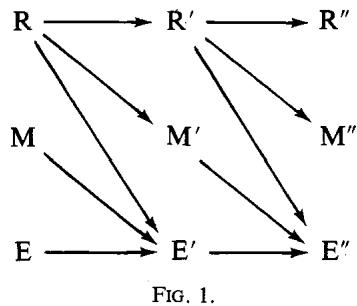
\includegraphics[keepaspectratio]{images/part001_66540ed3.jpg}}

通过上述同构，将H(Homgr \(_A\) (C, C'))等同于Ext (M, M')，同样地，将H(Homgr \(_A\) (C', C''))和H(Homgr \(_A\) (C, C''))也作相应等同，便得到七个同态。

\[
\operatorname{Ext} _ {\mathbf {A}} \left(\mathrm{M} ^ {\prime}, \mathrm{M} ^ {\prime \prime}\right) \otimes_ {k} \operatorname{Ext} _ {\mathbf {A}} \left(\mathrm{M}, \mathrm{M} ^ {\prime}\right)\rightarrow \operatorname{Ext} _ {\mathbf {A}} \left(\mathrm{M}, \mathrm{M} ^ {\prime \prime}\right).
\]

这七个同态彼此一致，并且与分解的选取无关。特别地，它们与第 2 号中通过三元组 (I(M), I(M'), I(M')) 所定义的同态一致。这确实可由将模 H(Homgr (C, C')) 解释为从复形 C 到 C' 的复形态射的同伦类所组成的模，以及以下事实得出：若在复形的一个图中

\[
\begin{array}{c} \mathrm{C} \xrightarrow {f} \mathrm{C} ^ {\prime} \xrightarrow {g} \mathrm{C} ^ {\prime \prime} \\ \alpha \Big \downarrow \qquad \qquad \alpha^ {\prime} \Big \downarrow \qquad \qquad \alpha^ {\prime \prime} \Big \downarrow \\ \mathrm{C} _ {1} \xrightarrow {f _ {1}} \mathrm{C} _ {1} ^ {\prime} \xrightarrow {g _ {1}} \mathrm{C} _ {1} ^ {\prime \prime} \end{array}
\]

\(\alpha'' \circ g\) 同伦于 \(g_1 \circ \alpha'\) ，而 \(\alpha' \circ f\) 同伦于 \(f_1 \circ \alpha\) ，则 \(\alpha'' \circ g \circ f\) 同伦于 \(g_1 \circ f_1 \circ \alpha\) （X，第 33 页，命题 4 及其推论）。

在下文中，我们将视情况使用上述七种复合同态构造中的某一种。

\subsection{与正合列相伴的类}

命题 1. --- 设 (C, d) 和 (C', d') 为两个左 A-模复形，n、p、q 为三个整数，使得 \(p \geqslant q\) 。对于 \(p \geqslant i \geqslant q - 1\) ，设 \(f_i: C_i \to C_{i+n+1}'\) 为一个 A-模同态，使得 \(f_p \circ d = 0\) ， \(f_i \circ d = d' \circ f_{i+1}\) （当 \(p > i \geqslant q - 1\) ），且 \(d' \circ f_{q-1} = 0\) （见图 2）。

\pandocbounded{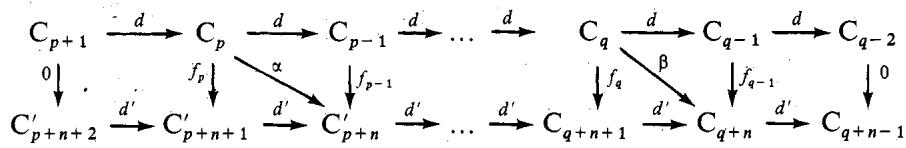
\includegraphics[keepaspectratio]{images/part001_b19b44e0.jpg}}\\
图 2。

令 \(\alpha = f_{p-1} \circ d = d' \circ f_p\) , \(\beta = f_{q-1} \circ d = d' \circ f_q\) ，并设 \(a\) (相应地， \(b\) )为从 C 到 C' 的度为 \(n\) 的分次 A-同态，其仅有的非零双齐次分量是 \(\alpha\) (相应地， \(\beta\) )。则有 \(a \in Z_n(\text{Homgr}_A(C, C'))\) , \(b \in Z_n(\text{Homgr}_A(C, C'))\) 和 \(a - (-1)^{(n+1)(p-q)} b \in B_n(\text{Homgr}_A(C, C'))\) 。

我们有 \(d' \circ \alpha = d' \circ d' \circ f_p = 0\) , \(\alpha \circ d = f_{p-1} \circ d \circ d = 0\) ，因此

\[
a \in Z _ {n} \left(\operatorname{Homgr} _ {\mathrm{A}} \left(\mathrm{C}, \mathrm{C} ^ {\prime}\right)\right);
\]

同理 \(b \in Z_n(\text{Homgr}_A(C, C'))\) 。令 \(\varepsilon = (-1)^{n+1}\) 。在复形 \(\text{Homgr}_A(C, C')\) 中有以下关系

\[
\mathrm{D} f _ {p - 1} = d ^ {\prime} \circ f _ {p - 1} - \varepsilon f _ {p - 1} \circ d = f _ {p - 2} \circ d - \varepsilon \alpha
\]

\[
\mathrm{D} f _ {i} = d ^ {\prime} \circ f _ {i} - \varepsilon f _ {i} \circ d = f _ {i - 1} \circ d - \varepsilon f _ {i} \circ d (p - 1 > i > q)
\]

\[
\mathrm{D} f _ {q} = d ^ {\prime} \circ f _ {q} - \varepsilon f _ {q} \circ d = \beta - \varepsilon f _ {q} \circ d,
\]

因此

\[
\sum_ {i = 1} ^ {p - q} \varepsilon^ {i} D f _ {p - i} = \varepsilon^ {p - q} \beta - \alpha ,
\]

这便证明了引理。

考虑两个左 A-模 M 与 N，以及一个 A-模正合列

\[
0 \rightarrow \mathrm{N} \rightarrow \mathrm{R} _ {n} \rightarrow \mathrm{R} _ {n - 1} \rightarrow \dots \rightarrow \mathrm{R} _ {1} \rightarrow \mathrm{M} \rightarrow 0.\tag{4}
\]

根据 X 第 49 页的命题 3 与命题 3 bis，存在一个交换图：

\begin{enumerate}
\def\labelenumi{(\arabic{enumi})}
\setcounter{enumi}{4}
\tightlist
\item
\end{enumerate}

\pandocbounded{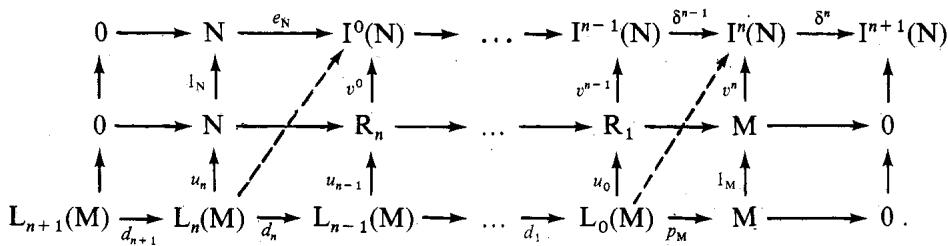
\includegraphics[keepaspectratio]{images/part001_efe78803.jpg}}

考虑这两个元素 \(b\) 与 \(a\) （它们属于 \(\mathrm{Homgr}_{\mathbf{A}}(\mathrm{L}(\mathbf{M}),\mathrm{I}(\mathbf{N}))\) ），其仅有的非零双齐次分量分别是

\[
b ^ {n} = e _ {\mathrm{N}} \circ u _ {n}: \mathrm{L} _ {n} (\mathrm{M}) \rightarrow \mathrm{I} ^ {0} (\mathrm{N}) \quad \text { and } \quad a ^ {n} = v ^ {n} \circ p _ {\mathrm{M}}: \mathrm{L} _ {0} (\mathrm{M}) \rightarrow \mathrm{I} ^ {n} (\mathrm{N})
\]

分别。

命题 2. --- 有 \(a\) , \(b \in Z^n(\text{Homgr}_A (\text{L(M)}, \text{l(N)})\) ）。此外，类 \(\overline{a}\) 与 \(\overline{b}\) ——即 \(a\) 与 \(b\) 的类——在 \(\text{H}^n(\text{Homgr}_A (\text{L(M)}, \text{l(N)})) = \text{Ext}_A^n (\text{M}, \text{N})\) 中仅依赖于正合列 (4)，并且相等。

将命题 1 应用于 (5) 中两端的行以及复合的竖直箭头，取 \(p = n\) , \(q = 0\) ，则有 \(a\) , \(b \in \mathbf{Z}^{n}(\mathrm{Homgr}_{\mathrm{A}}(\mathrm{l(M)}, \mathrm{L(N)}))\) ，并且

\[
a - b = a - (- 1) ^ {(n + 1) n} b \in \mathrm{B} ^ {n} (\operatorname{Homgr} _ {\mathrm{A}} (\mathrm{L} (\mathrm{M}), \mathrm{I} (\mathrm{N}))).
\]

由于 \(a\) （相应地， \(b\) ）与 \(u\) （相应地， \(v\) ）的选取无关，元素 \(\overline{a} = \overline{b}\) （属于 \(\mathrm{Ext}_{\mathbf{A}}^{n}\) (M, N)）与态射 \(u\) 和 \(v\) 的选取无关，由此得出该命题。

定义 1. --- 元素 \(\theta\) ，即 \(\operatorname{Ext}_{\mathbf{A}}^{n}(\mathbf{M}, \mathbf{N})\) 中由 \(\theta = (-1)^{n(n+1)/2} \overline{a} = (-1)^{n(n+1)/2} \overline{b}\) 所定义的元素，称为与正合列 (4) 相伴的类。

注记. --- 1) 设 (P, p) 是 M 的一个投射分解。由 X 第 49 页命题 3，存在一个交换图

\[
\begin{array}{c} 0 \longrightarrow \mathrm{N} \longrightarrow \mathrm{R} _ {n} \longrightarrow \dots \longrightarrow \mathrm{R} _ {1} \longrightarrow \mathrm{M} \longrightarrow 0 \\ \tilde {u} _ {n} \uparrow \quad \tilde {u} _ {n - 1} \uparrow \quad \tilde {u} _ {0} \uparrow \quad \uparrow_ {\mathrm{M}} \\ \mathrm{P} _ {n} \longrightarrow \mathrm{P} _ {n - 1} \longrightarrow \dots \longrightarrow \mathrm{P} _ {0} \xrightarrow {p} \mathrm{M} \longrightarrow 0. \end{array}
\]

使用 § 6 的记号，θ 是态射 P → N 的同伦类在 φ(P, N) 下的像，该态射由 \((-1)^{n(n+1)/2} \tilde{u}_{n}\) 定义。类似地，若 \((e, E)\) 是 N 的一个内射分解，则存在一个交换图

\[
\begin{array}{c} 0 \longrightarrow \mathrm{N} \longrightarrow \mathrm{E} ^ {0} \longrightarrow \dots \longrightarrow \mathrm{E} ^ {n - 1} \longrightarrow \mathrm{E} ^ {n} \\ 1 _ {\mathrm{N}} \uparrow \quad \tilde {v} ^ {0} \uparrow \quad \quad \quad \quad \quad \quad \quad \quad \quad \quad \quad \quad \quad \quad \quad \quad \quad \quad \quad \quad \quad \quad \quad \quad 0 \longrightarrow \mathrm{N} \longrightarrow \mathrm{R} _ {n} \longrightarrow \dots \longrightarrow \mathrm{R} _ {1} \longrightarrow \mathrm{M} \longrightarrow 0. \end{array}
\]

而 \(\theta\) 是 \(\varphi(\mathbf{M},\mathbf{E})\) 下态射 \(\mathbf{M}\to\mathbf{E}\) （由 \((-1)^{n(n+1)/2}v^{n}\) 定义）的同伦类的像。这由 \(\theta\) 的构造以及 \(\varphi(\mathbf{P},\mathbf{N})\) 与 \(\varphi(\mathbf{M},\mathbf{E})\) 的定义得出。

\begin{enumerate}
\def\labelenumi{\arabic{enumi})}
\setcounter{enumi}{1}
\tightlist
\item
  当 \(n = 0\) 时，正合列 (4) 写作 \(0 \to \mathbf{N} \xrightarrow{f} \mathbf{M} \to 0\) ，其相伴类为 \(f^{-1} \in \operatorname{Hom}_{\mathbf{A}}(\mathbf{M}, \mathbf{N}) = \operatorname{Ext}_{\mathbf{A}}^{0}(\mathbf{M}, \mathbf{N})\) 。
\end{enumerate}

\subsection{与正合列相伴的类的性质}

命题 3. --- 设

\begin{enumerate}
\def\labelenumi{(\arabic{enumi})}
\setcounter{enumi}{5}
\tightlist
\item
\end{enumerate}

\[
0 \rightarrow \mathrm{P} \rightarrow \mathrm{S} _ {m} \rightarrow \mathrm{S} _ {m - 1} \rightarrow \dots \rightarrow \mathrm{S} _ {1} \stackrel {\lambda_ {n}} {\rightarrow} \mathrm{N} \rightarrow 0\tag{7}
\]

\[
0 \rightarrow \mathrm{N} \xrightarrow {\mu} \mathrm{R} _ {n} \rightarrow \mathrm{R} _ {n - 1} \rightarrow \dots \rightarrow \mathrm{R} _ {1} \rightarrow \mathrm{M} \rightarrow 0
\]

为两个左 A-模正合列，其类分别为 \(\theta\in\mathrm{Ext}_{\mathbf{A}}^{m}(\mathbf{N},\mathbf{P})\) 与 \(\theta^{\prime}\in\mathrm{Ext}_{\mathbf{A}}^{n}(\mathbf{M},\mathbf{N})\) 。 \(\mathrm{Ext}_{\mathbf{A}}^{m+n}(\mathbf{M},\mathbf{P})\) 中与正合列

\[
0 \to \mathrm{P} \to \mathrm{S} _ {m} \to \dots \to \mathrm{S} _ {1} \xrightarrow {\mu \circ \lambda} \mathrm{R} _ {n} \to \dots \to \mathrm{R} _ {1} \to \mathrm{M} \to 0\tag{8}
\]

相伴的类是复合积 \(\theta\circ\theta'\) 。

选取交换图

\[
\begin{array}{c} 0 \longrightarrow \mathrm{P} \longrightarrow \mathrm{I} ^ {0} (\mathrm{P}) \longrightarrow \dots \longrightarrow \mathrm{I} ^ {m - 1} (\mathrm{P}) \xrightarrow {\delta_ {\mathrm{P}} ^ {m - 1}} \mathrm{I} ^ {m} (\mathrm{P}) \\ 0 \longrightarrow \mathrm{P} \longrightarrow \mathrm{S} _ {m} \longrightarrow \dots \longrightarrow \mathrm{S} _ {1} \xrightarrow {\lambda} \mathrm{N} \longrightarrow 0, \end{array}
\]

\[
\begin{array}{c c c c c c c c c c c c} 0 \longrightarrow & \mathrm{N} & \stackrel {{e _ {\mathrm{N}}}} {{\longrightarrow}} & \mathrm{I} ^ {0} (\mathrm{N}) & \longrightarrow & \dots & \longrightarrow & \mathrm{I} ^ {n - 1} (\mathrm{N}) & \longrightarrow & \mathrm{I} ^ {n} (\mathrm{N}) \\ & \uparrow_ {1 _ {\mathrm{N}}} & & v ^ {0} \uparrow & & & & v ^ {n - 1} \uparrow & & v ^ {n} \uparrow \\ 0 \longrightarrow & \mathrm{N} & \stackrel {{\mu}} {{\longrightarrow}} & \mathrm{R} _ {n} & \longrightarrow & \dots & \longrightarrow & \mathrm{R} _ {1} & \longrightarrow & \mathrm{M} & \longrightarrow & 0. \end{array}
\]

由于 \(\mathrm{I}^{m}(\mathrm{P})\) 是内射的，存在同态 \(h^{0}: \mathrm{I}^{0}(\mathrm{N}) \to \mathrm{I}^{m}(\mathrm{P})\) 使得 \(w^{m} = h^{0} \circ e_{N}\) ；由 X 第 49 页命题 3 bis， \(h^{0}\) 可延拓为复形的态射 \(h: \mathrm{I}(\mathrm{N}) \to \mathrm{I}(\mathrm{P})(-m)\) 。于是 \(w^{m} = h^{0} \circ e_{N} = h^{0} \circ v^{0} \circ \mu\) ，因此

\[
\delta_ {1} ^ {m - 1} \circ w ^ {m - 1} = w ^ {m} \circ \lambda = h ^ {0} \circ v ^ {0} \circ (\mu \circ \lambda),
\]

且下图是交换的：

\[
\begin{array}{l}0 \longrightarrow \mathrm{P} \longrightarrow \mathrm{I} ^ {0} (\mathrm{P}) \longrightarrow \dots \longrightarrow \mathrm{I} ^ {m - 1} (\mathrm{P}) \longrightarrow \mathrm{I} ^ {m} (\mathrm{P}) \longrightarrow \mathrm{I} ^ {m + 1} (\mathrm{P}) \longrightarrow \dots \longrightarrow \mathrm{I} ^ {m + n} (\mathrm{P})\\0 \longrightarrow \mathrm{P} \longrightarrow \mathrm{S} _ {m} \longrightarrow \dots \longrightarrow \mathrm{S} _ {1} \underset {\mu \circ \lambda} {\longrightarrow} \mathrm{R} _ {n} \longrightarrow \mathrm{R} _ {n - 1} \longrightarrow \dots \longrightarrow \mathrm{M} \rightarrow 0\end{array}
\]

其中 \(t^0 = h^0 \circ v^0\) , \(t^1 = (-1)^m h^1 \circ v^1, \ldots, t^i = (-1)^{mi} h^i \circ v^i, \ldots, t^n = (-1)^{mn} h^n \circ v^n\) 。与 (6) 相伴的类 \(\theta\) 是 \((-1)^{m(m+1)/2} w^m \in \text{Homgr}_A^m(\mathbf{N}, \mathbf{l}(\mathbf{P}))\) 的类，因此经同构 \(a_{\mathbf{N},\mathbf{P}}\) 对应于 \((-1)^{m(m+1)/2} h \in \text{Homgr}_A^m(\mathbf{l}(\mathbf{N}), \mathbf{l}(\mathbf{P}))\) 的类；与 (7) 相伴的类 \(\theta'\) 是 \((-1)^{n(n+1)/2} v^n \in \text{Homgr}_A^m(\mathbf{M}, \mathbf{l}(\mathbf{N}))\) 的类，与 (8) 相伴的类是 \((-1)^{(m+n)(m+n+1)/2} t^n \in \text{Homgr}_{m+n}^m(\mathbf{M}, \mathbf{l}(\mathbf{P}))\) 的类，于是由复合积的定义（X，第 114 页）及公式得出结论

\[
m (m + 1) / 2 + n (n + 1) / 2 = (m + n) (m + n + 1) / 2 - m n.
\]

\begin{enumerate}
\def\labelenumi{\arabic{enumi}.}
\setcounter{enumi}{3}
\tightlist
\item
  --- 考虑一个 A-模的交换图，它具有正合
\end{enumerate}

行

\pandocbounded{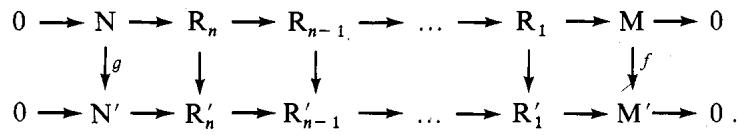
\includegraphics[keepaspectratio]{images/part001_b790ce53.jpg}}

设 θ（相应地，θ′）为第一行（相应地，第二行）在下式中的类

\[
\operatorname{Ext} _ {\mathbf {A}} ^ {n} (\mathbf {M}, \mathbf {N}) \quad \left(\text { resp.   } \operatorname{Ext} _ {\mathbf {A}} ^ {n} (\mathbf {M} ^ {\prime}, \mathbf {N} ^ {\prime})\right).
\]

在 \(\operatorname{Ext}_{\mathbf{A}}^{n}(\mathbf{M}, \mathbf{N}')\) 中，有 \(\theta' \circ f = g \circ \theta\) 。

事实上，考虑一个交换图

\pandocbounded{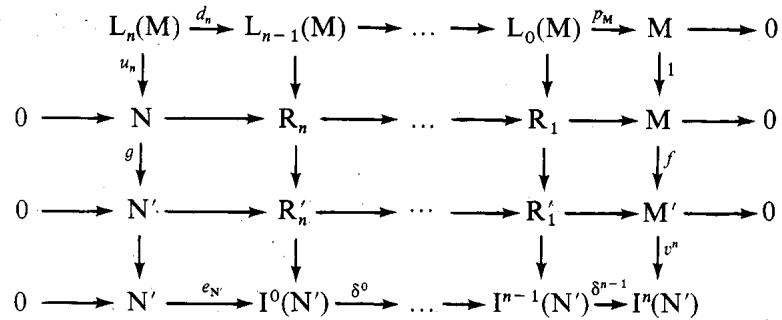
\includegraphics[keepaspectratio]{images/part001_126cf8d3.jpg}}

根据定义， \(\theta' \circ f\) 是 \((-1)^{n(n+1)/2} v^n \circ f \circ p_M \in \text{Homgr}^n (\text{L(M)}, \text{I(N')})\) 的类，而 \(g \circ \theta\) 是 \((-1)^{n(n+1)/2} e_{N'} \circ g \circ u_n\) 的类。将引理 1 应用于该图两端的行，这两个类相等。

推论 1. --- 考虑一个具有正合行的交换图

\[
\begin{array}{c c c c c c c c} 0 \longrightarrow & \mathrm{N} \longrightarrow & \mathrm{R} _ {n} \longrightarrow & \dots & \longrightarrow & \mathrm{R} _ {1} \longrightarrow & \mathrm{M} \longrightarrow & 0 \\ & ^ {1} \downarrow & & & \downarrow & & ^ {1} \downarrow \\ 0 \longrightarrow & \mathrm{N} \longrightarrow & \mathrm{R} _ {n} ^ {\prime} \longrightarrow & \dots & \longrightarrow & \mathrm{R} _ {1} ^ {\prime} \longrightarrow & \mathrm{M} \longrightarrow & 0; \end{array}
\]

图的两行在 \(\operatorname{Ext}_{\mathbf{A}}^{n}(\mathbf{M},\mathbf{N})\) 中有相同的相伴类。

推论 2. --- 设

\[
0 \rightarrow \mathrm{N} \xrightarrow {f _ {n - 1}} \mathrm{R} _ {n} \xrightarrow {f _ {n}} \mathrm{R} _ {n - 1} \rightarrow \dots \xrightarrow {f _ {2}} \mathrm{R} _ {1} \xrightarrow {f _ {1}} \mathrm{M} \rightarrow 0
\]

是一个正合列， \(\theta\in\mathrm{Ext}_{\mathbf{A}}^{n}(\mathbf{M},\mathbf{N})\) 为其相伴的类， \(a_{1},\ldots,a_{n+1}\) 为 \(k\) 的可逆元。与正合列

\[
0 \rightarrow \mathrm{N} \xrightarrow {a _ {n + 1} f _ {n + 1}} \mathrm{R} _ {n} \xrightarrow {a _ {n} f _ {n}} \mathrm{R} _ {n - 1} \rightarrow \dots \xrightarrow {a _ {2} f _ {2}} \mathrm{R} _ {1} \xrightarrow {a _ {1} f _ {1}} \mathrm{M} \rightarrow 0
\]

相伴的类是 \((a_{1}^{-1}a_{2}^{-1}\dots a_{n + 1}^{-1})\theta .\)

事实上，我们有一个交换图

\[
\begin{array}{c} 0 \longrightarrow \mathrm{N} \xrightarrow {a _ {n + 1} f _ {n + 1}} \mathrm{R} _ {n} \longrightarrow \dots \longrightarrow \mathrm{R} _ {2} \xrightarrow {a _ {2} f _ {2}} \mathrm{R} _ {1} \xrightarrow {a _ {1} f _ {1}} \mathrm{M} \longrightarrow 0 \\ \Biggl \downarrow a _ {1} \dots a _ {n + 1} \quad \Biggl \downarrow a _ {1} \dots a _ {n} \quad \Biggl \downarrow a _ {1} a _ {2} \quad \Biggl \downarrow a _ {1} \quad \Biggl \downarrow 1 \\ 0 \longrightarrow \mathrm{N} \xrightarrow {f _ {n + 1}} \mathrm{R} _ {n} \longrightarrow \dots \longrightarrow \mathrm{R} _ {2} \xrightarrow {f _ {2}} \mathrm{R} _ {1} \xrightarrow {f _ {1}} \mathrm{M} \longrightarrow 0. \end{array}
\]

然后应用该命题。

推论 3. --- 设 \(0 \to \mathbf{N} \xrightarrow{f_{n+1}} \mathbf{R}_{n} \xrightarrow{f_{n}} \cdots \to \mathbf{R}_{1} \xrightarrow{f_{1}} \mathbf{M} \to 0\) 为一个正合列， \(\theta\) 为它在 \(\operatorname{Ext}_{\mathbf{A}}^{n}(\mathbf{M}, \mathbf{N})\) 中的类， \(u: \mathbf{M}' \to \mathbf{M}\) 与 \(v: \mathbf{N} \to \mathbf{N}'\) 为两个 A-模同态。

\begin{enumerate}
\def\labelenumi{\alph{enumi})}
\tightlist
\item
  元素 \(v \circ \theta\) （属于 \(\operatorname{Ext}_{\mathbf{A}}^{n}(\mathbf{M}, \mathbf{N}')\) ）等于正合列
\end{enumerate}

\[
0 \rightarrow \mathrm{N} ^ {\prime} \xrightarrow {f _ {n + 1} ^ {\prime}} \mathrm{R} _ {n} ^ {\prime} \xrightarrow {f _ {n} ^ {\prime}} \mathrm{R} _ {n - 1} \xrightarrow {f _ {n - 1}} \dots \rightarrow \mathrm{R} _ {1} \rightarrow \mathrm{M} \rightarrow 0,
\]

的类，其中 \(R_{n}^{\prime}\) 是 A-模 \(R_{n} \oplus N^{\prime}\) 除以由诸对 \((f_{n+1}(x), -v(x))\) （ \(x \in N\) ）所构成的子模而得的商模，而 \(f_{n+1}^{\prime}\) (相应地， \(f_{n}^{\prime}\) )由典范单射（相应地，由 \((f_{n}, 0)\) ）通过取商得到。

\begin{enumerate}
\def\labelenumi{\alph{enumi})}
\setcounter{enumi}{1}
\tightlist
\item
  元素 \(\theta \circ u\) （属于 \(\operatorname{Ext}_{\mathbf{A}}^{n}(\mathbf{M}^{\prime}, \mathbf{N})\) ）是正合列
\end{enumerate}

\[
0 \rightarrow \mathrm{N} \rightarrow \mathrm{R} _ {n} \rightarrow \dots \rightarrow \mathrm{R} _ {2} \xrightarrow {f _ {2} ^ {\prime \prime}} \mathrm{R} _ {1} ^ {\prime} \xrightarrow {f _ {1} ^ {\prime \prime}} \mathrm{M} ^ {\prime} \rightarrow 0,
\]

的类，其中 \(R_{1}^{\prime}\) 是纤维积 \(R_{1} \times_{M} M^{\prime}\) ，亦即（I，第 44 页） \(R_{1} \times M^{\prime}\) 中由对 \((x, y)\) （满足 \(f_{1}(x) = u(y)\) ）所构成的子模，而 \(f_{2}^{\prime\prime}\) (相应地， \(f_{1}^{\prime\prime}\) )由 \((f_{2}, 0)\) （相应地，由第二个投影）导出。

例如，我们来证明 \(a\) )。设 \(z\) 为 \(\mathbf{R}_{n}^{\prime}\) 中满足 \(f_{n}^{\prime}(z)=0\) 的一个元素；若 \(z\) 是对 \((x,y)\) 的类，其中 \(x\in\mathbf{R}_{n},y\in\mathbf{N}^{\prime}\) ，则有 \(f_{n}(x)=0\) ，从而存在元素 \(t\in\mathbf{N}\) 使得 \(x=f_{n+1}(t)\) 。于是有 \(z=f_{n+1}^{\prime}(y+v(t))\) ，这就证明了 \(\operatorname{Ker} f_{n}^{\prime}=\operatorname{Im} f_{n+1}^{\prime}\) 。 \(f_{n+1}^{\prime}\) 的单射性由 \(f_{n+1}\) 的单射性得出。

设 \(j: \mathbf{R}_{n} \to \mathbf{R}_{n}^{\prime}\) 为由典范单射导出的同态；我们有正合列的交换图：

\[
\begin{array}{c} 0 \longrightarrow \mathrm{N} \xrightarrow {f _ {n + 1}} \mathrm{R} _ {n} \xrightarrow {f _ {n}} \mathrm{R} _ {n - 1} \longrightarrow \dots \longrightarrow \mathrm{M} \longrightarrow 0 \\ \Biggl \downarrow v \quad \Biggl \downarrow j \quad \Biggl \downarrow 1 \\ 0 \longrightarrow \mathrm{N} ^ {\prime} \xrightarrow {f _ {n + 1} ^ {\prime}} \mathrm{R} _ {n} ^ {\prime} \xrightarrow {f _ {n} ^ {\prime}} \mathrm{R} _ {n - 1} \longrightarrow \dots \longrightarrow \mathrm{M} \longrightarrow 0; \end{array}
\]

于是断言 a) 由该命题得出。

 \(b\) 的证明是类似的。

注记。--- 设 \(\theta\in\mathrm{Ext}_{\mathbf{A}}^{n}(\mathbf{M},\mathbf{N})\) ，分别地 \(\theta^{\prime}\in\mathrm{Ext}_{\mathbf{A}}^{n}(\mathbf{M}^{\prime},\mathbf{N}^{\prime})\) ，是正合序列的类

\[
0 \rightarrow \mathrm{N} \xrightarrow {f _ {n + 1}} \mathrm{R} _ {n} \rightarrow \dots \rightarrow \mathrm{R} _ {1} \xrightarrow {f _ {1}} \mathrm{M} \rightarrow 0,
\]

\[
\text { resp. } 0 \to \mathrm{N} ^ {\prime} \xrightarrow {f _ {n + 1} ^ {\prime}} \mathrm{R} _ {n} ^ {\prime} \to \dots \to \mathrm{R} _ {1} ^ {\prime} \xrightarrow {f _ {1} ^ {\prime}} \mathrm{M} ^ {\prime} \to 0.
\]

设 \(i_{\mathbf{N}}, i_{\mathbf{N}'}\) 为 \(\mathbf{N}\) 与 \(\mathbf{N}'\) 到 \(\mathbf{N} \oplus \mathbf{N}'\) 中的典范单射， \(q_{\mathbf{M}}\) , \(q_{\mathbf{M}'}\) 为 \(\mathbf{M} \oplus \mathbf{M}'\) 到 \(\mathbf{M}\) 与 \(\mathbf{M}'\) 上的投影。考虑同态

\[
m = \operatorname{Ext} \left(q _ {\mathbf {M}}, i _ {\mathbf {N}}\right) \oplus \operatorname{Ext} \left(q _ {\mathbf {M} ^ {\prime}}, i _ {\mathbf {N} ^ {\prime}}\right)
\]

是从 \(\operatorname{Ext}_{\mathbf{A}}(\mathbf{M},\mathbf{N})\oplus \operatorname{Ext}_{\mathbf{A}}(\mathbf{M}^{\prime},\mathbf{N}^{\prime})\) 到 \(\operatorname{Ext}_{\mathbf{A}}(\mathbf{M}\oplus \mathbf{M}^{\prime},\mathbf{N}\oplus \mathbf{N}^{\prime}\) 的同态。元素

\[
m (\theta , \theta^ {\prime}) = i _ {\mathrm{N}} \circ \theta \circ q _ {\mathrm{M}} + i _ {\mathrm {N^ {\prime}}} \circ \theta^ {\prime} \circ q _ {\mathrm {M^ {\prime}}}
\]

是正合列

\[
0 \rightarrow \mathrm{N} \oplus \mathrm{N} ^ {\prime} \xrightarrow {f _ {n + 1} \oplus f _ {n - 1} ^ {\prime}} \mathrm{R} _ {n} \oplus \mathrm{R} _ {n} ^ {\prime} \rightarrow \dots \rightarrow \mathrm{R} _ {1} \oplus \mathrm{R} _ {1} ^ {\prime} \xrightarrow {f _ {1} \oplus f _ {1} ^ {\prime}} \mathrm{M} \oplus \mathrm{M} ^ {\prime} \rightarrow 0.
\]

的类。事实上，若将这个类记为 \(\theta''\) ，则由命题 4 可知，有

\[
\theta^ {\prime \prime} \circ i _ {\mathrm{M}} = i _ {\mathrm{N}} \circ \theta = m (\theta , \theta^ {\prime}) \circ i _ {\mathrm{M}} \quad \text {and} \quad \theta^ {\prime \prime} \circ i _ {\mathrm{M} ^ {\prime}} = i _ {\mathrm{N} ^ {\prime}} \circ \theta = m (\theta , \theta^ {\prime}) \circ i _ {\mathrm{M} ^ {\prime}};
\]

根据 X 第 89 页命题 7，这意味着 \(\theta'' = m(\theta, \theta')\) 。

\subsection{\texorpdfstring{正合列与 Ext 元素之间的关系 \(_{A}\) (M, N)}{正合列与 Ext 元素之间的关系 \_\{A\} (M, N)}}

定理 1. --- 设 n 为整数 ≥1，M 和 N 为两个 A-模。

\begin{enumerate}
\def\labelenumi{\alph{enumi})}
\item
  Ext \(_{A}^{n}\) (M, N) 的每个元素都是某个正合列的类（X，第 117 页，定义 1）。
\item
  设 \(0 \to \mathbf{N} \xrightarrow{f_{n+1}} \mathbf{R}_n \xrightarrow{f_n} \ldots \to \mathbf{R}_1 \xrightarrow{f_1} \mathbf{M} \to 0\)
\end{enumerate}

和

\[
0 \rightarrow \mathrm{N} \xrightarrow {f _ {n + 1} ^ {\prime}} \mathrm{R} _ {n} ^ {\prime} \xrightarrow {f _ {n} ^ {\prime}} \dots \rightarrow \mathrm{R} _ {1} ^ {\prime} \xrightarrow {f _ {1} ^ {\prime}} \mathrm{M} \rightarrow 0
\]

为两个正合列， \(\theta\) 与 \(\theta'\) 为其相伴的类。以下条件等价：

\begin{enumerate}
\def\labelenumi{(\roman{enumi})}
\item
  \(\theta = \theta^{\prime}\) ;
\item
  存在一个具有正合行的交换图：
\end{enumerate}

\[
\begin{array}{c} 0 \longrightarrow \mathrm{N} \xrightarrow {f _ {n + 1}} \mathrm{R} _ {n} \longrightarrow \dots \longrightarrow \mathrm{R} _ {1} \xrightarrow {f _ {1}} \mathrm{M} \longrightarrow 0 \\ 0 \longrightarrow \mathrm{N} \longrightarrow \mathrm{R} _ {n} ^ {\prime \prime} \longrightarrow \dots \longrightarrow \mathrm{R} _ {1} ^ {\prime} \longrightarrow \mathrm{M} \longrightarrow 0 \\ 0 \longrightarrow \mathrm{N} \xrightarrow {f _ {n + 1} ^ {\prime}} \mathrm{R} _ {n} ^ {\prime} \longrightarrow \dots \longrightarrow \mathrm{R} _ {1} ^ {\prime} \xrightarrow {f _ {1} ^ {\prime}} \mathrm{M} \longrightarrow 0; \end{array}
\]

\begin{enumerate}
\def\labelenumi{(\roman{enumi})}
\setcounter{enumi}{2}
\tightlist
\item
  存在一个具有正合行的交换图：
\end{enumerate}

\[
\begin{array}{c} 0 \longrightarrow \mathrm{N} \xrightarrow {f _ {n + 1}} \mathrm{R} _ {n} \longrightarrow \dots \longrightarrow \mathrm{R} _ {1} \xrightarrow {f _ {1}} \mathrm{M} \longrightarrow 0 \\ 0 \longrightarrow \mathrm{N} \longrightarrow \mathrm{R} _ {n} ^ {\prime \prime} \longrightarrow \dots \longrightarrow \mathrm{R} _ {1} ^ {\prime \prime} \longrightarrow \mathrm{M} \longrightarrow 0 \\ 0 \longrightarrow \mathrm{N} \xrightarrow {f _ {n + 1} ^ {\prime}} \mathrm{R} _ {n} ^ {\prime} \longrightarrow \dots \longrightarrow \mathrm{R} _ {1} ^ {\prime} \xrightarrow {f _ {1} ^ {\prime}} \mathrm{M} \longrightarrow 0. \end{array}
\]

我们来证明 \(a\) )。设 \(\alpha \in \operatorname{Ext}_{\mathbf{A}}^{n}(\mathbf{M}, \mathbf{N})\) ，并设 \(\mathbf{P}\) 为 \(\mathbf{M}\) 的一个投射分解。设 \(a: \mathrm{P}(n) \to \mathbf{N}\) 为表示 \(\alpha\) 的复形态射；其唯一的非零分量是一个 A-同态 \(u: \mathrm{P}_{n} \to \mathbf{N}\) ，它满足 \(u \circ d_{n+1} = 0\) ，因此有分解 \(u = \overline{u} \circ \delta_{n}\) ，其中 \(\delta_{n}: \mathrm{P}_{n} \to \dot{\mathbf{Z}}_{n-1}\) 是由 \(d_{n}\) 诱导的映射（我们设 \(Z_{n-1} = \operatorname{Im} d_{n}\) ），而 \(\overline{u}\) 是从 \(Z_{n-1}\) 到 \(\mathbf{N}\) 的一个 A-同态。根据第 117 页的注记 1，类 \(\theta \in \operatorname{Ext}_{\mathbf{A}}^{n}(\mathbf{M}, Z_{n-1})\) ——即正合列

\[
0 \rightarrow Z _ {n - 1} \rightarrow P _ {n - 1} \rightarrow \dots \rightarrow P _ {0} \rightarrow M \rightarrow 0
\]

的类——等于态射 \((-1)^{n(n + 1) / 2}\delta_n\) 的同伦类。因此我们有

\[
\alpha = (- 1) ^ {n (n + 1) / 2} \overline {{{u}}} \circ \theta ,
\]

根据第 120 页的推论 3，由此可将 α 表示为某个正合列的类。

由 X 第 120 页的推论 1 可知，(ii) \(\Rightarrow\) (i) 且 (iii) \(\Rightarrow\) (i)。假设 (i) 成立，并设 P 为 M 的一个投射分解。存在一个交换图

\[
\begin{array}{c} 0 \longrightarrow \mathrm{N} \xrightarrow {f _ {n + 1}} \mathrm{R} _ {n} \longrightarrow \mathrm{R} _ {n - 1} \longrightarrow \dots \longrightarrow \mathrm{R} _ {1} \longrightarrow \mathrm{M} \longrightarrow 0 \\ u _ {n} \uparrow \quad \uparrow u _ {n - 1} \quad \uparrow u _ {n - 2} \quad \uparrow \quad \uparrow_ {\mathrm{I} _ {\mathrm{M}}} \\ \mathrm{P} _ {n} \xrightarrow {d _ {n}} \mathrm{P} _ {n - 1} \longrightarrow \mathrm{P} _ {n - 2} \longrightarrow \dots \longrightarrow \mathrm{P} _ {0} \longrightarrow \mathrm{M} \longrightarrow 0 \\ u _ {n} ^ {\prime} \downarrow \quad \downarrow u _ {n - 1} ^ {\prime} \quad \downarrow u _ {n - 2} ^ {\prime} \quad \downarrow \quad \downarrow_ {\mathrm{I} _ {\mathrm{M}}} \\ 0 \longrightarrow \mathrm{N} \xrightarrow {f _ {n + 1}} \mathrm{R} _ {n} ^ {\prime} \longrightarrow \mathrm{R} _ {n - 1} ^ {\prime} \longrightarrow \dots \longrightarrow \mathrm{R} _ {1} ^ {\prime} \longrightarrow \mathrm{M} \longrightarrow 0. \end{array}
\]

从 \(\mathrm{P}(n)\) 到 \(\mathbf{N}\) 的、由 \(u_{n}\) 与 \(u_{n}^{\prime}\) 定义的态射是同伦的，因为它们都属于类 \((-1)^{n(n + 1) / 2}\theta\) ，因此 \(u_{n}^{\prime} - u_{n}\) 具有 \(w\circ d_n\) 的形式，其中 \(w:\mathrm{P}_{n - 1}\to \mathrm{N}\) 是一个 A-同态。将 \(u_{n - 1}^{\prime}\) 换为 \(u_{n - 1}^{\prime} - f_{n + 1}^{\prime}\circ w\) ，并将 \(u_{n}^{\prime}\) 换为 \(u_{n}\) ，就可归结为 \(u_{n} = u_{n}^{\prime}\) 的情形。这使得我们可以构造一个新的具有正合行的交换图：

\[
\begin{array}{c c c c c c c} 0 \longrightarrow \mathrm{N} \longrightarrow \mathrm{R} _ {n} \longrightarrow \mathrm{R} _ {n - 1} \longrightarrow \dots \longrightarrow \mathrm{R} _ {1} \longrightarrow \mathrm{M} \longrightarrow 0 \\ 1 _ {\mathrm{N}} \uparrow & \uparrow v & \uparrow u _ {n - 2} & \uparrow & \uparrow^ {1 _ {\mathrm{M}}} \\ 0 \longrightarrow \mathrm{N} \longrightarrow \mathrm{N} ^ {\prime} \longrightarrow \mathrm{P} _ {n - 2}. \longrightarrow \dots \longrightarrow \mathrm{P} _ {0} \longrightarrow \mathrm{M} \longrightarrow 0 \\ 1 _ {\mathrm{N}} \downarrow & \downarrow v ^ {\prime} & \downarrow u _ {n - 2} ^ {\prime} & \downarrow & \downarrow^ {1 _ {\mathrm{M}}} \\ 0 \longrightarrow \mathrm{N} \longrightarrow \mathrm{R} _ {n} ^ {\prime} \longrightarrow \mathrm{R} _ {n - 1} ^ {\prime} \longrightarrow \dots \longrightarrow \mathrm{R} _ {1} ^ {\prime} \longrightarrow \mathrm{M} \longrightarrow 0 \end{array}
\]

其中 \(\mathbf{N}'\) 是 \(\mathbf{P}_{n-1} \oplus \mathbf{N}\) 除以由诸对 \((d_n(x), -u_n(x))\) （ \(x \in \mathbf{P}_n\) ）所构成的子模而得的商模，而 \(v\) (相应地， \(v'\) )是由映射 \(u_{n-1} \oplus f_{n+1}\) （相应地， \(u_{n-1}' \oplus f_{n+1}'\) ）通过取商定义的。因此条件 (ii) 得到满足。

再假设条件 (i) 成立，并设 E 为 N 的一个内射分解。存在一个交换图

\[
\begin{array}{c c c c c c c} 0 \longrightarrow \mathrm{N} \longrightarrow \mathrm{R} _ {n} \longrightarrow & \dots \longrightarrow \mathrm{R} _ {1} \longrightarrow \mathrm{M} \longrightarrow & 0 \\ 1 _ {\mathrm{N}} \Big \downarrow & \Big \downarrow v _ {0} & v _ {n - 1} \Big \downarrow & \Big \downarrow v _ {n} \\ 0 \longrightarrow \mathrm{N} ^ {\prime} \longrightarrow \mathrm{E} ^ {0} \stackrel {{\delta^ {0}}} {{\longrightarrow}} & \dots \longrightarrow \mathrm{E} ^ {n - 1} \stackrel {{\delta^ {n - 1}}} {{\longrightarrow}} \mathrm{E} ^ {n} \\ 1 _ {\mathrm{N}} \Big \uparrow & \Big \uparrow v _ {0} ^ {\prime} & v _ {n - 1} ^ {\prime} \Big \uparrow & \Big \uparrow v _ {n} ^ {\prime} \\ 0 \longrightarrow \mathrm{N} \longrightarrow \mathrm{R} _ {n} ^ {\prime} \longrightarrow & \dots \longrightarrow \mathrm{R} _ {1} ^ {\prime} \longrightarrow & \mathrm{M} \longrightarrow & 0 \end{array}
\]

并且如上面所示，可以假设 \(v_{n}^{\prime}=v_{n}\) 。于是我们有一个具有正合行的交换图

\[
\begin{array}{c c c c c c c c} 0 \longrightarrow N \longrightarrow R _ {n} \longrightarrow \dots \longrightarrow R _ {2} \longrightarrow R _ {1} \longrightarrow M \longrightarrow 0 \\ \downarrow^ {1 _ {N}} & \downarrow & & \downarrow & \downarrow & \downarrow^ {1 _ {M}} \\ 0 \longrightarrow N \longrightarrow E ^ {0} \longrightarrow \dots \longrightarrow E ^ {n - 2} \longrightarrow M ^ {\prime} \longrightarrow M \longrightarrow 0 \\ \uparrow^ {1 _ {N}} & \uparrow & & \uparrow & \uparrow & \uparrow^ {1 _ {M}} \\ 0 \longrightarrow N \longrightarrow R _ {n} ^ {\prime} \longrightarrow \dots \longrightarrow R _ {2} ^ {\prime} \longrightarrow R _ {1} ^ {\prime} \longrightarrow M \longrightarrow 0 \end{array}
\]

其中 \(\mathbf{M}' = \mathbf{M} \times_{\mathrm{R}_{1}} \mathbf{E}_{n-1}\) （参见 X，第 120 页，推论 3，b））。因此条件 (iii) 成立，这就完成了定理的证明。

注记 1. --- 若环 A 是诺特环，且 A-模 M 与 N 都是有限生成的，则由 a) 的证明可知，Ext \(_{A}^{n}\) (M, N) 的每个元素都是与某个正合列 0 → N → R \(_{n}\) → \ldots{} → R \(_{1}\) → M → 0 相伴的类，其中诸 R \(_{i}\) 都是有限生成的。

推论. --- 设 \(0 \to \mathbf{N} \xrightarrow{f} \mathbf{R} \xrightarrow{g} \mathbf{M} \to 0\) 与 \(0 \to \mathbf{N} \xrightarrow{f'} \mathbf{R}' \xrightarrow{g'} \mathbf{M} \to 0\) 为两个正合列， \(\theta\) 与 \(\theta'\) 为它们在 \(\operatorname{Ext}^1(\mathbf{M}, \mathbf{N})\) 中的相伴类。为使 \(\theta = \theta'\) ，必须且只需存在一个 A-同态 \(h: \mathbf{R} \to \mathbf{R}'\) 使得图表

\[
\begin{array}{c} \mathsf {R} \\ \mathsf {N} \\ \mathsf {f ^ {\prime}} \end{array} \begin{array}{c} \mathsf {f} \\ \mathsf {h} \\ \mathsf {R ^ {\prime}} \end{array} \begin{array}{c} \mathsf {g} \\ \mathsf {M} \\ \mathsf {g ^ {\prime}} \end{array}
\]

交换的。这样的同态必然是一个同构。

由命题 4 的推论 1，该条件是充分的。若 \(\theta = \theta'\) ，则我们有一个具有正合行的交换图：

\[
\begin{array}{c} 0 \longrightarrow \mathrm{N} \longrightarrow \mathrm{R} \longrightarrow \mathrm{M} \longrightarrow 0 \\ \uparrow_ {1 _ {\mathrm{N}}} \Big | _ {h ^ {\prime}} \Big | _ {1 _ {\mathrm{M}}} \\ 0 \longrightarrow \mathrm{N} \longrightarrow \mathrm{R} ^ {\prime \prime} \longrightarrow \mathrm{M} \longrightarrow 0 \\ \uparrow_ {1 _ {\mathrm{N}}} \Big | _ {h ^ {\prime \prime}} \Big | _ {1 _ {\mathrm{M}}} \\ 0 \longrightarrow \mathrm{N} \longrightarrow \mathrm{R} ^ {\prime} \longrightarrow \mathrm{M} \longrightarrow 0. \end{array}
\]

态射 \(h'\) 与 \(h''\) 由 X 第 7 页推论 3 知是同构，且 \(h = h'' \circ h'^{-1}\) 回答了该问题。最后一个断言由同上引文得出。

注记 2. --- 定理 1 把 Ext \(_{A}^{n}\) (M, N) 描述为正合列的等价类集合；通过结构转移，容易描述在此集合上得到的群法则。事实上，设 θ（相应地，θ′）为正合列 0 → N \(\xrightarrow{f_{n+1}}\) R \(_{n}\) \(\xrightarrow{f_n}\) \ldots{} → R \(_{1}\) → M → 0（相应地，0 → N \(\xrightarrow{f_{n+1}'}\) R \(_{n}'\) \(\xrightarrow{f_n'}\) \ldots{} → R \(_{1}'\) → M → 0）的类。设 Δ : M → M ⊕ M 与 ∇ : N ⊕ N → N 为 A-线性映射，由 Δ(x) = (x, x)（x ∈ M）与 ∇(y, z) = y + z（y, z ∈ N）定义。考虑映射

\[
m: \operatorname{Ext} _ {\mathbf {A}} (\mathbf {M}, \mathbf {N}) \oplus \operatorname{Ext} _ {\mathbf {A}} (\mathbf {M}, \mathbf {N}) \rightarrow \operatorname{Ext} _ {\mathbf {A}} (\mathbf {M} \oplus \mathbf {M}, \mathbf {N} \oplus \mathbf {N})
\]

是在第 121 页的注记中定义的。采用同上引文的记号，我们有 \(\nabla \circ i_{\mathbf{N}} = 1_{\mathbf{N}}\) 和 \(q_{\mathbf{M}} \circ \Delta = 1_{\mathbf{M}}\) ，从而 \(\theta + \theta' = \nabla \circ m(\theta, \theta') \circ \Delta\) 。鉴于同上引文及第 120 页的推论 3，这就给出一个类为 \(\theta + \theta'\) 的正合列：例如，若 \(n \geqslant 2\) ，可取序列

\[
0 \rightarrow \mathrm{N} \rightarrow \mathrm{R} _ {n} ^ {\prime \prime} \rightarrow \mathrm{R} _ {n - 1} \oplus \mathrm{R} _ {n - 1} ^ {\prime} \xrightarrow {f _ {n - 1} \oplus f _ {n - 1} ^ {\prime}} \dots \rightarrow \mathrm{R} _ {2} \oplus \mathrm{R} _ {2} ^ {\prime} \rightarrow \mathrm{R} _ {1} ^ {\prime \prime} \rightarrow \mathrm{M} \rightarrow 0
\]

其中 \(R_{n}^{\prime\prime}\) 是 \(R_{n} \oplus R_{n}^{\prime}\) 除以由诸对

\[
\left(f _ {n + 1} (x), - f _ {n + 1} ^ {\prime} (x)\right) \quad \text { for } x \in \mathbf {N},
\]

所构成的子模而得的商模，且其中 \(R_{1}^{\prime\prime}=R_{1}\times_{M}R_{1}^{\prime}\)
% semantic-fragments: legacy-input-seam
\relax{}
\subsection{复合积与扩张模的连接同态}

命题 5. --- 设

\[
0 \to {\bf M} ^ {\prime} \stackrel {f} {\to} {\bf M} \stackrel {g} {\to} {\bf M} ^ {\prime \prime} \to 0\tag{8}
\]

是左A-模的一个正合序列， \(\theta\in\mathrm{Ext}_{\mathbf{A}}^{1}\left(\mathbf{M}^{\prime\prime},\mathbf{M}^{\prime}\right)\) 为相应的类，N为左A-模，n为整数。

\begin{enumerate}
\def\labelenumi{\alph{enumi})}
\item
  连接同态 \(\delta^{n}(\mathbf{N},\mathcal{E}):\operatorname{Ext}_{\mathbf{A}}^{n}(\mathbf{N},\mathbf{M}^{\prime \prime})\to \operatorname{Ext}_{\mathbf{A}}^{n + 1}(\mathbf{N},\mathbf{M}^{\prime})\) 是复合积 \(\alpha \mapsto \theta \circ \alpha\) ，即用 \(\theta\) 作复合而得.
\item
  连接同态 \(\delta^{n}(\mathcal{E},\mathbf{N}):\operatorname{Ext}_{\mathbf{A}}^{n}(\mathbf{M}^{\prime},\mathbf{N})\to\operatorname{Ext}_{\mathbf{A}}^{n+1}(\mathbf{M}^{\prime\prime},\mathbf{N})\) 是复合积 \(\alpha\mapsto(-1)^{n+1}\alpha\circ\theta\) ，即用 \((-1)^{n+1}\theta\) 作复合而得.
\item
  考虑一个交换图
\end{enumerate}

\[
\begin{array}{l} 0 \xrightarrow {} \mathrm{M} ^ {\prime} \xrightarrow {f} \mathrm{M} \xrightarrow {g} \mathrm{M} ^ {\prime \prime} \xrightarrow {} 0 \\ 0 \xrightarrow {} \mathrm{M} ^ {\prime} \xrightarrow {e _ {\mathrm{M} ^ {\prime}}} \mathrm{I} ^ {0} (\mathrm{M} ^ {\prime}) \xrightarrow {\delta^ {0}} \mathrm{I} ^ {1} (\mathrm{M} ^ {\prime}). \end{array}
\]

根据定义， \(\theta\) 是 \(-v^{1}\in\mathrm{Homgr}_{\mathbf{A}}^{1}(\mathbf{M}^{\prime\prime},\mathbf{I}(\mathbf{M}^{\prime}))\) 的类。再设 \(\alpha\in\mathrm{Ext}_{\mathbf{A}}^{n}(\mathbf{N},\mathbf{M}^{\prime\prime})\) ，它由元素 \(a\) （属于 \(\mathrm{Homgr}_{\mathbf{A}}^{n}(\mathbf{L}(\mathbf{N}),\mathbf{M}^{\prime\prime})\) ）来表示。根据构造， \(\delta^{n}(\alpha)\) 如下获得：将 \(a^{n}\in\mathrm{Hom}_{\mathbf{A}}(\mathbf{L}_{n}(\mathbf{N}),\mathbf{M}^{\prime\prime})\) 提升为

\[
b \in \operatorname{Hom} _ {\mathbf {A}} \left(\mathrm{L} _ {n} (\mathrm{N}), \mathrm{M}\right),
\]

而 \(\delta^n (\alpha)\) 是 \(e_{\mathbf{M}'}\circ c\) 的类，其中 \(c\in \mathrm{Hom}_{\mathbf{A}}\left(\mathbf{L}_{n + 1}(\mathbf{N}),\mathbf{M}'\right)\) 满足

\[
f \circ c = \mathrm{D} b = (- 1) ^ {n + 1} b \circ d _ {n + 1}.
\]

因此我们有一个交换图

\[
\begin{array}{c} L _ {n + 1} (N) \xrightarrow {d _ {n + 1}} L _ {n} (N) \\ (- 1) ^ {n + 1} c \Big \downarrow \\ 0 \longrightarrow M ^ {\prime} \xrightarrow {f} M \xrightarrow {g} M ^ {\prime \prime} \longrightarrow 0 \\ 1 _ {M ^ {\prime}} \Big \downarrow \\ 0 \longrightarrow M ^ {\prime} \xrightarrow {e _ {M ^ {\prime}}} I ^ {0} (M ^ {\prime}) \xrightarrow {\delta^ {0}} I ^ {1} (M ^ {\prime}). \end{array}
\]

但在 \(\operatorname{Homgr}_{\mathbf{A}}(\mathbf{L}(\mathbf{N}), \mathbf{l}(\mathbf{M}'))\) 中，我们有

\[
\mathrm{D} \left(v ^ {0} \circ b\right) = \delta^ {0} \circ v ^ {0} \circ b - (- 1) ^ {n} v ^ {0} \circ b \circ d _ {n + 1} = v ^ {1} \circ a ^ {n} + e _ {\mathrm{M} ^ {\prime}} \circ c.
\]

\(e_{\mathbf{M}'} \circ c\) 与 \((-v^1) \circ a\) 的类在 \(\operatorname{Ext}_{\mathbf{A}}^{n+1}(\mathbf{N}, \mathbf{M}')\) 中相等，由此得 \(a\) ).

\begin{enumerate}
\def\labelenumi{\alph{enumi})}
\setcounter{enumi}{1}
\tightlist
\item
  考虑一个交换图
\end{enumerate}

\[
\begin{array}{c} \mathrm{L} _ {1} (\mathrm{M} ^ {\prime \prime}) \xrightarrow {d _ {1}} \mathrm{L} _ {0} (\mathrm{M} ^ {\prime \prime}) \xrightarrow {p _ {\mathrm{M} ^ {\prime \prime}}} \mathrm{M} ^ {\prime \prime} \longrightarrow 0 \\ \Biggl \downarrow u _ {1} \\ 0 \longrightarrow \mathrm{M} ^ {\prime} \xrightarrow {f} \mathrm{M} \xrightarrow {g} \mathrm{M} ^ {\prime \prime} \longrightarrow 0. \end{array}
\]

根据定义， \(\theta\) 是 \(-u_{1}\in\mathrm{Homgr}_{\mathbf{A}}^{1}(\mathrm{L}(\mathbf{M}^{\prime\prime}),\mathbf{M}^{\prime})\) 的类。再设 \(\alpha\in\mathrm{Ext}^{n}(\mathbf{M}^{\prime},\mathbf{N})\) ，它由元素 \(a\) （属于 \(\mathrm{Homgr}_{\mathbf{A}}^{n}(\mathbf{M}^{\prime},\mathrm{I}(\mathbf{N}))\) ）来表示。根据构造， \(\delta^{n}(\alpha)\) 如下获得：将 \(a^{n}\in\mathrm{Hom}_{\mathbf{A}}(\mathbf{M}^{\prime},\mathrm{I}^{n}(\mathbf{N}))\) 扩充为

\[
b \in \operatorname{Hom} _ {\mathbf {A}} (\mathbf {M}, \mathrm{I} ^ {n} (\mathbf {N}))
\]

而 \(\delta^n (\alpha)\) 是 \(c\circ p_{\mathbf{M}''}\) 的类，其中 \(c\in \mathrm{Hom}_{\mathbf{A}}(\mathbf{M}^{\prime \prime},\mathrm{I}^{n + 1}(\mathbf{N}))\) 满足

\[
g \circ c = D b = \delta^ {n + 1} \circ b.
\]

因此我们有一个交换图

\[
\begin{array}{c} L _ {1} (M ^ {\prime \prime}) \xrightarrow {d _ {1}} L _ {0} (M ^ {\prime \prime}) \xrightarrow {p _ {M ^ {\prime \prime}}} M ^ {\prime \prime}. \longrightarrow 0 \\ u _ {1} \Biggl \downarrow \quad \quad \quad \quad \quad \quad \quad \quad \quad \quad \quad \quad \quad \quad \quad \quad \quad \quad \quad \quad \quad \quad \quad \quad \quad \quad \quad \quad \quad \quad \quad \quad \quad \quad \quad \quad \quad \quad \quad \quad \quad \quad \quad \quad \quad \quad \quad 1 _ {M ^ {\prime}} \\ 0 \longrightarrow M ^ {\prime} \xrightarrow {f} M \xrightarrow {g} M ^ {\prime \prime} \longrightarrow 0 \\ a ^ {n} \Biggl \downarrow \quad \quad \quad \quad \quad \quad \quad \quad \quad \quad \quad \quad c \Biggl \downarrow \\ I ^ {n} (N) \xrightarrow {\delta^ {n}} I ^ {n + 1} (N). \end{array}
\]

但在 \(\operatorname{Homgr}_{\mathbf{A}}(\mathbf{L}(\mathbf{M}^{\prime \prime}),\mathbf{l}(\mathbf{N}))\) 中，我们有

\[
\mathrm{D} (b \circ u _ {0}) = \delta^ {n} \circ b \circ u _ {0} - (- 1) ^ {n} b \circ u _ {0} \circ c = c \circ p - (- 1) ^ {n} a ^ {n} \circ u _ {1}.
\]

\(c \circ p\) 与 \((-1)^{n+1} a^n \circ (-u_1)\) 的类在 \(\operatorname{Ext}_{\mathbf{A}}^{n+1} (\mathbf{M}''\) , \(\mathbf{N}\) ) 中因此相等，由此得 \(b\) ).

推论 1. --- a) 连接同态 Hom \(_{A}\) (M'', M'') → Ext \(_{A}^{1}\) (M'', M') 将 1 \(_{M''}\) 映至 θ。

\begin{enumerate}
\def\labelenumi{\alph{enumi})}
\setcounter{enumi}{1}
\tightlist
\item
  连接同态 \(\operatorname{Hom}_{\mathbf{A}}(\mathbf{M}^{\prime},\mathbf{M}^{\prime})\to\operatorname{Ext}_{\mathbf{A}}^{1}(\mathbf{M}^{\prime\prime},\mathbf{M}^{\prime})\) 将 \(1_{M'}\) 映至 \(-\theta\).
\end{enumerate}

推论 2. --- 考虑左 A-模的两个正合序列

\[
0 \rightarrow \mathbf {M} ^ {\prime} \rightarrow \mathbf {M} \rightarrow \mathbf {M} ^ {\prime \prime} \rightarrow 0
\]

\[
0 \rightarrow \mathrm{N} ^ {\prime} \rightarrow \mathrm{N} \rightarrow \mathrm{N} ^ {\prime \prime} \rightarrow 0.
\]

则连接同态的复合同态

\[
\operatorname{Ext} _ {\mathbf {A}} ^ {n} \left(\mathrm{M} ^ {\prime}, \mathrm{N} ^ {\prime \prime}\right)\rightarrow \operatorname{Ext} _ {\mathbf {A}} ^ {n + 1} \left(\mathrm{M} ^ {\prime \prime}, \mathrm{N} ^ {\prime \prime}\right)\rightarrow \operatorname{Ext} _ {\mathbf {A}} ^ {n + 2} \left(\mathrm{M} ^ {\prime \prime}, \mathrm{N} ^ {\prime}\right)
\]

与

\[
\operatorname{Ext} _ {\mathbf {A}} ^ {n} \left(\mathrm{M} ^ {\prime}, \mathrm{N} ^ {\prime \prime}\right)\rightarrow \operatorname{Ext} _ {\mathbf {A}} ^ {n + 1} \left(\mathrm{M} ^ {\prime}, \mathrm{N} ^ {\prime}\right)\rightarrow \operatorname{Ext} _ {\mathbf {A}} ^ {n + 2} \left(\mathrm{M} ^ {\prime \prime}, \mathrm{N} ^ {\prime}\right)
\]

是相反的。

事实上，若 \(\theta_{1}\) , \(\theta_{2}\) 是与给定正合序列相关联的类，且若 \(\alpha \in \operatorname{Ext}_{\mathbf{A}}^{n}(\mathbf{M}', \mathbf{M}'')\) ，则 \(\alpha\) 的像分别为

\[
\theta_ {2} \circ ((- 1) ^ {n + 1} \alpha \circ \theta_ {1}) \quad \text { and } \quad (\theta_ {2} \circ \alpha) \circ ((- 1) ^ {n + 2} \theta_ {1}).
\]

考虑左 A-模的一个正合序列

\[
0 \rightarrow \mathrm{N} \rightarrow \mathrm{R} _ {n} \xrightarrow {f _ {n}} \mathrm{R} _ {n - 1} \xrightarrow {f _ {n - 1}} \dots \rightarrow \mathrm{R} _ {1} \xrightarrow {f _ {1}} \mathrm{M} \rightarrow 0\tag{S}
\]

并设 \(K_{0} = M\) , \(K_{i} = Ker f_{i}, i = 1, \ldots, n - 1\) , \(K_{n} = N\) 。因此我们有正合序列

\[
0 \to \mathbf {K} _ {i} \to \mathbf {R} _ {i} \to \mathbf {K} _ {i - 1} \to 0, \quad 1 \leqslant i \leqslant n,\tag{9}
\]

与之相关联的，对每个左 A-模 P，有连接同态

\[
\begin{array}{r l}&{\mathrm{Ext} _ {\mathbf {A}} ^ {m} \left(\mathrm{P}, \mathbf {K} _ {i - 1}\right)\rightarrow \mathrm{Ext} _ {\mathbf {A}} ^ {m + 1} \left(\mathrm{P}, \mathbf {K} _ {i}\right),}\\&{\qquad \mathrm{Ext} _ {\mathbf {A}} ^ {m} \left(\mathbf {K} _ {i}, \mathrm{P}\right)\rightarrow \mathrm{Ext} _ {\mathbf {A}} ^ {m + 1} \left(\mathbf {K} _ {i - 1}, \mathrm{P}\right),}\end{array}
\]

从而通过迭代连接同态的复合，与 (S) 相关联

\[
\begin{array}{l} \delta^ {m} (\mathrm{P}, \mathcal {S}): \operatorname{Ext} _ {\mathrm{A}} ^ {m} (\mathrm{P}, \mathrm{M}) \to \operatorname{Ext} _ {\mathrm{A}} ^ {m + n} (\mathrm{P}, \mathrm{N}) \\ \delta^ {m} (\mathcal {S}, \mathrm{P}): \operatorname{Ext} _ {\mathrm{A}} ^ {m} (\mathrm{N}, \mathrm{P}) \to \operatorname{Ext} _ {\mathrm{A}} ^ {m + n} (\mathrm{M}, \mathrm{P}). \end{array}
\]

推论 3. --- 如果 \(\theta\in\mathrm{Ext}_{\mathbf{A}}^{n}(\mathbf{M},\mathbf{N})\) 是与正合序列 \((\mathcal{S})\) 相关联的类，则我们有

\[
\delta^ {m} (\mathrm{P}, \mathscr {S}) (\alpha) = \theta \circ \alpha , \quad \delta^ {m} (\mathscr {S}, \mathrm{P}) (\beta) = (- 1) ^ {m n + n (n + 1) / 2} \beta \circ \theta .
\]

若 \(\theta_{i}\in\mathrm{Ext}_{\mathbf{A}}^{1}(\mathbf{K}_{i-1},\mathbf{K}_{i})\) 是与正合序列 (9) 相关联的类，根据命题 5，我们有

\[
\begin{array}{l} \delta^ {m} (\mathrm{P}, \mathcal {S}) (\alpha) = \theta_ {n} \circ \dots \circ \theta_ {2} \circ \theta_ {1} \circ \alpha \\ \delta^ {m} (\mathcal {S}, \mathrm{P}) (\beta) = (- 1) ^ {(m + 1) + \dots + (m + n)} \beta \circ \theta_ {n} \circ \dots \circ \theta_ {1}. \end{array}
\]

此外，根据命题 3（X，第 118 页），我们有 \(\theta = \theta_{n} \circ \cdots \circ \theta_{1}\) 。推论立即由此及关系式（E，III，第44页）得出

\[
(m + 1) + \dots + (m + n) = m n + n (n + 1) / 2.
\]

推论4. --- 若每个模 \(\mathbf{R}_i\) , \(i = 1, \ldots, n\) 都是内射的（相应地，投射的），则映射 \(\alpha \mapsto \theta \circ \alpha\) （相应地， \(\alpha \mapsto \alpha \circ \theta\) ）从 \(\operatorname{Ext}_{\mathbf{A}}^{m}(\mathbf{P}, \mathbf{M})\) 到 \(\operatorname{Ext}_{\mathbf{A}}^{m+n}(\mathbf{P}, \mathbf{N})\) （相应地，从 \(\operatorname{Ext}_{\mathbf{A}}^{m}(\mathbf{N}, \mathbf{P})\) 到 \(\operatorname{Ext}_{\mathbf{A}}^{m+n}(\mathbf{M}, \mathbf{P})\) ）对每个 A-模 P 和每个整数 \(m > 0\) 都是双射的。这确实由推论 3 及正合序列

\[
\operatorname{Ext} _ {\mathbf {A}} ^ {m + i - 1} \left(\mathrm{P}, \mathrm{R} _ {i}\right)\rightarrow \operatorname{Ext} _ {\mathbf {A}} ^ {m + i - 1} \left(\mathrm{P}, \mathrm{K} _ {i - 1}\right)\rightarrow \operatorname{Ext} _ {\mathbf {A}} ^ {m + i} \left(\mathrm{P}, \mathrm{K} _ {i}\right)\rightarrow \operatorname{Ext} _ {\mathbf {A}} ^ {m + i} \left(\mathrm{P}, \mathrm{R} _ {i}\right)
\]

\[
\left(\text { resp. } \operatorname{Ext} _ {\mathbf {A}} ^ {m + i - 1} \left(\mathrm{R} _ {i}, \mathrm{P}\right)\rightarrow \operatorname{Ext} _ {\mathbf {A}} ^ {m + i - 1} \left(\mathrm{K} _ {i}, \mathrm{P}\right)\rightarrow \operatorname{Ext} _ {\mathbf {A}} ^ {m + i} \left(\mathrm{K} _ {i - 1}, \mathrm{P}\right)\rightarrow \operatorname{Ext} _ {\mathbf {A}} ^ {m + i} \left(\mathrm{R} _ {i}, \mathrm{P}\right)\right),
\]

得出，其两端项按假设为零。

注记. --- 第3至6节的定义和命题适用于右A-模，它们被视为环A的反环A°上的左模。

\subsection{\texorpdfstring{同态 \(\operatorname{Ext}_{\mathbf{A}}(\mathbf{P}, \mathbf{Q}) \otimes \operatorname{Tor}^{\mathbf{A}}(\mathbf{P}, \mathbf{M}) \to \operatorname{Tor}^{\mathbf{A}}(\mathbf{Q}, \mathbf{M})\)}{同态 \textbackslash operatorname\{Ext\}\_\{\textbackslash mathbf\{A\}\}(\textbackslash mathbf\{P\}, \textbackslash mathbf\{Q\}) \textbackslash otimes \textbackslash operatorname\{Tor\}\^{}\{\textbackslash mathbf\{A\}\}(\textbackslash mathbf\{P\}, \textbackslash mathbf\{M\}) \textbackslash 到 \textbackslash operatorname\{Tor\}\^{}\{\textbackslash mathbf\{A\}\}(\textbackslash mathbf\{Q\}, \textbackslash mathbf\{M\})}}

设 M 为左 A-模，P 与 Q 为两个右 A-模。考虑同态 \(\operatorname{Homgr}_{\mathbf{A}}(\mathrm{L}(\mathrm{P}), \mathrm{L}(\mathrm{Q})) \otimes_{k} (\mathrm{L}(\mathrm{P}) \otimes_{\mathbf{A}} \mathrm{L}(\mathrm{M})) \to \mathrm{L}(\mathrm{Q}) \otimes_{\mathbf{A}} \mathrm{L}(\mathrm{M})\) 它将 \(f \otimes (x \otimes y)\) 映至 \(f(x) \otimes y\) 。根据X，第99页，这是复形的一个态射。由此可推出一个 0 次的分次 \(k\) -线性映射

\[
\mathrm{H} (\operatorname{Homgr} _ {\mathrm{A}} (\mathrm{L} (\mathrm{P}), \mathrm{L} (\mathrm{Q}))) \otimes_ {k} \operatorname{Tor} ^ {\mathrm{A}} (\mathrm{P}, \mathrm{M}) \rightarrow \operatorname{Tor} ^ {\mathrm{A}} (\mathrm{Q}, \mathrm{M})
\]

因此，经由 § 6（X，第100页，定理1）的同构 \(\varphi(\mathbf{L}(\mathbf{P}),\mathbf{L}(\mathbf{Q}))\) ，得到一个 0 次的分次 \(k\) -线性映射

\[
\operatorname{Ext} _ {\mathbf {A}} (\mathrm{P}, \mathrm{Q}) \otimes_ {k} \operatorname{Tor} ^ {\mathbf {A}} (\mathrm{P}, \mathrm{M}) \rightarrow \operatorname{Tor} ^ {\mathbf {A}} (\mathrm{Q}, \mathrm{M}),\tag{10}
\]

对应于k-双线性映射

\[
c _ {\mathrm{P}, \mathrm{Q}; \mathrm{M}}: \operatorname{Ext} _ {\mathrm{A}} ^ {n} (\mathrm{P}, \mathrm{Q}) \times \operatorname{Tor} _ {m} ^ {\mathrm{A}} (\mathrm{P}, \mathrm{M}) \rightarrow \operatorname{Tor} _ {m - n} ^ {\mathrm{A}} (\mathrm{Q}, \mathrm{M});\tag{11}
\]

偶 \((\alpha, \gamma)\) 在 \(c_{P,Q;M}\) 下的像称为 \(\alpha\) 与 \(\gamma\) 的复合积，记作 \(\alpha \circ \gamma\) .

按构造， \(\alpha \circ \gamma\) 如下获得： \(\alpha\) 由复形的态射 \(f: \mathrm{L}(\mathrm{P}) \to \mathrm{L}(\mathrm{Q})(-n)\) 表示， \(\gamma\) 由元素 \(z \in Z_m(\mathrm{L}(\mathrm{P}) \otimes_{\mathbf{A}} \mathrm{L}(\mathrm{M}))\) 表示，则 \(\alpha \otimes \gamma\) 是元素

\[
(f \otimes 1) (z) \in Z _ {m} (\mathrm{L} (\mathrm{Q}) (- n) \otimes_ {\mathrm{A}} \mathrm{L} (\mathrm{M})) = Z _ {m - n} (\mathrm{L} (\mathrm{Q}) \otimes_ {\mathrm{A}} \mathrm{L} (\mathrm{M})).
\]

例如，如果 \(\alpha \in \operatorname{Hom}_{\mathbf{A}}(\mathbf{P},\mathbf{Q})\) ，则 \(\alpha \circ \gamma = \operatorname{Tor}(\alpha,1)(\gamma)\) .

注记. --- 1) 若使用 X，第 69 页的同构 \(\psi\) ，则也可通过交换图定义复合积

\[
\begin{array}{c} \operatorname{Ext} _ {\mathrm{A}} ^ {n} (\mathrm{P}, \mathrm{Q}) \times \operatorname{Tor} _ {m} ^ {\mathrm{A}} (\mathrm{P}, \mathrm{M}) \xrightarrow {c _ {\mathrm{P} , \mathrm{Q} : \mathrm{M}}} \operatorname{Tor} _ {m - n} ^ {\mathrm{A}} (\mathrm{Q}, \mathrm{M}) \\ \bar {a} _ {\mathrm{P}, \mathrm{Q}} \times \psi_ {\mathrm{P}} (\mathrm{M}) \Biggl \downarrow \\ \mathrm{H} ^ {n} (\operatorname{Homgr} _ {\mathrm{A}} (\mathrm{L} (\mathrm{P}), \mathrm{L} (\mathrm{Q}))) \times \mathrm{H} _ {m} (\mathrm{L} (\mathrm{P}) \otimes_ {\mathrm{A}} \mathrm{M}) \longrightarrow \mathrm{H} _ {m - n} (\mathrm{L} (\mathrm{Q}) \otimes_ {\mathrm{A}} \mathrm{M}); \end{array}
\]

换言之，我们将 \(\alpha\) 表示为态射 \(f\) ：从 L(P) 到 L(Q) \((-n)\) ，将 \(\gamma\) 表示为循环 \(x \in \mathrm{L}_{m}(\mathrm{P}) \otimes_{\mathbf{A}} \mathrm{M}\) ，且 \(\alpha \circ \gamma\) 是下述元素的循环类

\[
\left(f _ {m} \otimes 1 _ {\mathbf {M}}\right) (x) \in \mathrm{L} _ {m - n} (\mathrm{Q}) \otimes_ {\mathbf {A}} \mathrm{M}.
\]

\begin{enumerate}
\def\labelenumi{\arabic{enumi})}
\setcounter{enumi}{1}
\tightlist
\item
  也可以使用分解 I(P) 和 I(Q)。
\end{enumerate}

类似地，如果 N 是第二个左 A-模，则可定义复合积 \((\mu, \gamma) \mapsto \mu \circ \gamma\) ，记作

\[
c _ {\mathrm{P}; \mathrm{M}, \mathrm{N}}: \operatorname{Ext} _ {\mathrm{A}} ^ {r} (\mathrm{M}, \mathrm{N}) \times \operatorname{Tor} _ {m} ^ {\mathrm{A}} (\mathrm{P}, \mathrm{M}) \rightarrow \operatorname{Tor} _ {m - r} ^ {\mathrm{A}} (\mathrm{P}, \mathrm{N})
\]

由交换图

\[
\begin{array}{c} \operatorname{Ext} _ {\mathbf {A}} ^ {r} (\mathbf {M}, \mathbf {N}) \times \operatorname{Tor} _ {m} ^ {\mathbf {A}} (\mathbf {P}, \mathbf {M}) \xrightarrow {c _ {\mathrm{P} ; \mathrm{M} , \mathrm{N}}} \operatorname{Tor} _ {m - r} ^ {\mathbf {A}} (\mathbf {P}, \mathbf {N}) \\ 1 \times \sigma_ {\mathrm{P}, \mathrm{M}, r} \Biggl \downarrow \\ \operatorname{Ext} _ {\mathbf {A} ^ {\circ}} ^ {r} (\mathbf {M} ^ {\circ}, \mathbf {N} ^ {\circ}) \times \operatorname{Tor} _ {m} ^ {\mathbf {A} ^ {\circ}} (\mathbf {M} ^ {\circ}, \mathbf {P} ^ {\circ}) \xrightarrow {c _ {\mathrm{M} ^ {\circ} , \mathrm{N} ^ {\circ} ; \mathrm{P} ^ {\circ}}} \operatorname{Tor} _ {m - r} ^ {\mathbf {A} ^ {\circ}} (\mathbf {N} ^ {\circ}, \mathbf {P} ^ {\circ}) \end{array}\tag{12}
\]

其中 σ 表示交换同构（X，第 71 页）。

若 \(\mu \in \operatorname{Ext}_{\mathbf{A}}^{r}(\mathbf{M}, \mathbf{N})\) 是态射 \(g: \mathrm{L}(\mathbf{M}) \to \mathrm{L}(\mathbf{N})(-r)\) 的类，且 \(\gamma \in \operatorname{Tor}_{m}^{\mathbf{A}}(\mathbf{P}, \mathbf{M})\) 是 \(z = \sum_{i,j} z_{ij}\) 的循环类，其中 \(z_{ij} \in \mathrm{L}_i(\mathbf{P}) \otimes_{\mathbf{A}} \mathrm{L}_j(\mathbf{M})\) ，则 \(\mu \circ \gamma\) 就是循环 \(\sum_{i,j} (-1)^{ir}(1 \otimes g)(z_{ij})\) 的类 .

我们还可以将 \(\gamma\) 表示为一个循环 \(y \in \mathrm{P} \otimes \mathrm{L}_{m}(\mathbf{M})\) ，且 \(\mu \circ \gamma\) 是 \((1 \otimes g)(y) \in \mathrm{P} \otimes \mathrm{L}_{m-r}(\mathbf{M})\) 的循环类 .

命题 6. --- 设 K、M、N 为左 A-模，P、Q、R 为右 A-模，

\[
\alpha \in \operatorname{Ext} _ {\mathrm{A}} ^ {n} (\mathrm{P}, \mathrm{Q}), \beta \in \operatorname{Ext} _ {\mathrm{A}} ^ {p} (\mathrm{Q}, \mathrm{R}), \lambda \in \operatorname{Ext} _ {\mathrm{A}} ^ {r} (\mathrm{K}, \mathrm{M}), \mu \in \operatorname{Ext} _ {\mathrm{A}} ^ {s} (\mathrm{M}, \mathrm{N}), \gamma \in \operatorname{Tor} _ {m} ^ {\mathrm{A}} (\mathrm{P}, \mathrm{K}).
\]

则

\begin{enumerate}
\def\labelenumi{(\arabic{enumi})}
\setcounter{enumi}{12}
\tightlist
\item
\end{enumerate}

\[
(\beta \circ \alpha) \circ \gamma = \beta \circ (\alpha \circ \gamma) \text { in }\operatorname{Tor} _ {m - p - n} ^ {\mathrm{A}} (\mathrm{R}, \mathrm{K}),\tag{14}
\]

\[
(\mu \circ \lambda) \circ \gamma = \mu \circ (\lambda \circ \gamma) \text { in }\operatorname{Tor} _ {n - r - s} ^ {\mathbf {A}} (\mathrm{P}, \mathrm{N}),\tag{15}
\]

\[
\alpha \circ (\lambda \circ \gamma) = (- 1) ^ {n r} \lambda \circ (\alpha \circ \gamma) \text { in }\operatorname{Tor} _ {m - p - r} ^ {\mathrm{A}} (\mathrm{Q}, \mathrm{M}).
\]

公式（13）和（14）直接由定义得出。我们来证明（15）。设 \(z = \sum z_{ij}, z_{ij} \in \mathbf{L}_i(\mathbf{P}) \otimes \mathbf{L}_j(\mathbf{K})\) 为表示 \(\gamma, f: \mathrm{L}(\mathrm{P}) \to \mathrm{L}(\mathrm{Q})(-n)\) 与 \(g: \mathbf{L}(\mathbf{K}) \to \mathbf{L}(\mathbf{M})(-r)\) 的循环与态射，它们分别表示 \(\alpha\) 与 \(\lambda\) 。则 \(\lambda \circ (\alpha \circ \gamma)\) 是 \(\sum (-1)^{(i-n)r}(f \otimes g)(z_{ij})\) 的类，而 \(\alpha \circ (\lambda \circ \gamma)\) 是

\[
\sum (- 1) ^ {i r} (f \otimes g) (z _ {i j}), \quad \text { whence } (1 5).
\]

\subsection{复合积与挠积的连接同态}

命题 7. --- a) 设

\[
0 \to \mathrm{P} ^ {\prime} \xrightarrow {f} \mathrm{P} \xrightarrow {g} \mathrm{P} ^ {\prime \prime} \to 0\tag{8}
\]

是右 A-模的一个正合序列， \(\theta\in\mathrm{Ext}_{\mathrm{A}}^{1}\left(\mathrm{P}^{\prime\prime},\mathrm{P}^{\prime}\right)\) 为相应的类，M 为左 A-模。连接同态

\[
\delta_ {n} (\mathcal {E}, \mathrm{M}): \operatorname{Tor} _ {n} ^ {\mathrm{A}} \left(\mathrm{P} ^ {\prime \prime}, \mathrm{M}\right)\rightarrow \operatorname{Tor} _ {n - 1} ^ {\mathrm{A}} \left(\mathrm{P} ^ {\prime}, \mathrm{M}\right) \quad \text { is the map } \quad\gamma \mapsto \theta \circ \gamma .
\]

\begin{enumerate}
\def\labelenumi{\alph{enumi})}
\setcounter{enumi}{1}
\tightlist
\item
  设
\end{enumerate}

\[
0 \rightarrow \mathrm{M} ^ {\prime} \rightarrow \mathrm{M} \rightarrow \mathrm{M} ^ {\prime \prime} \rightarrow 0\tag{$(\mathcal{E}_1)$}
\]

是左 A-模的一个正合序列， \(\theta_{1} \in \operatorname{Ext}_{\mathbf{A}}^{1}(\mathbf{M}^{\prime \prime}, \mathbf{M}^{\prime})\) 为相应的类，P 为右 A-模。连接同态

\[
\delta_ {n} (\mathrm{P}, \mathcal {E} _ {1}): \operatorname{Tor} _ {n} ^ {\mathrm{A}} (\mathrm{P}, \mathrm{M} ^ {\prime \prime}) \rightarrow \operatorname{Tor} _ {n - 1} ^ {\mathrm{A}} (\mathrm{P}, \mathrm{M} ^ {\prime}) \quad \text { is the map } \quad\gamma \mapsto \theta_ {1} \circ \gamma .
\]

设 \(\gamma\in\mathrm{Tor}_{n}^{\mathrm{A}}(\mathrm{P}^{\prime\prime},\mathrm{M})\) 为闭链 \(z^{\prime\prime}\in\dot{\mathrm{Z}}_{n}(\mathrm{L}(\mathrm{P}^{\prime\prime})\otimes_{\mathrm{A}}\mathrm{L}(\mathrm{M}))\) 的类，并设

\[
\begin{array}{c} 0 \longrightarrow \mathrm{P} ^ {\prime} \xrightarrow {f} \mathrm{P} \xrightarrow {g} \mathrm{P} ^ {\prime \prime} \longrightarrow 0 \\ \uparrow_ {u _ {1}} \quad \uparrow_ {u _ {0}} \quad \uparrow_ {1} \\ \mathrm{L} _ {1} (\mathrm{P} ^ {\prime \prime}) \xrightarrow {d _ {1}} \mathrm{L} _ {0} (\mathrm{P} ^ {\prime \prime}) \xrightarrow {p _ {0} ^ {\prime \prime}} \mathrm{P} ^ {\prime \prime} \longrightarrow 0 \end{array}
\]

为一个交换图。我们将用 \(p' : \mathrm{L}(\mathrm{P}') \to \mathrm{P}'\) 和 \(p'' : \mathrm{L}(\mathrm{P}''') \to \mathrm{P}''\) 表示复形的典范态射。根据定义， \(\delta(\gamma) \in \mathrm{Tor}_{n-1}^{\mathrm{A}}(\mathrm{P}', \mathrm{M})\) 如下获得：选取 \(x \in \mathrm{P} \otimes \mathrm{L}_n(\mathrm{M})\) 使得 \((g \otimes 1)(x) = (p'' \otimes 1)(z'')\) ，而 \(\delta(\gamma)\) 是使得下式成立的循环 \(z' \in Z_{n-1}(\mathrm{L}(\mathrm{P}') \otimes \mathrm{L}(\mathrm{M}))\) 的类

\[
(f \otimes 1) (p ^ {\prime} \otimes 1) (z ^ {\prime}) = (1 \otimes d _ {n}) (x).
\]

对于 \(0 \leqslant i \leqslant n\) ，设 \(z_{i}^{\prime \prime}\) 为 \(z^{\prime \prime}\) 在 \(\mathrm{L}_{i}(\mathrm{P}^{\prime \prime}) \otimes \mathrm{L}_{n - i}(\mathrm{M})\) 中的分量；我们有

\[
0 = \mathrm{D} z ^ {\prime \prime} = \sum_ {i} \left(d _ {i} \otimes 1 + (- 1) ^ {i} \otimes d _ {n - i}\right) (z _ {i} ^ {\prime \prime}),
\]

\(\mathrm{donc}(d_i \otimes 1)(z_i'') = (-1)^i \otimes d_{n-i+1}(z_{i-1}'')\) 并且特别地

\[
\left(d _ {1} \otimes 1\right) \left(z _ {1} ^ {\prime \prime}\right) = - 1 \otimes d _ {n} \left(z _ {0} ^ {\prime \prime}\right).
\]

于是我们选择 \(x = (u_0 \otimes 1)(z_0'')\) ：我们确实有

\[
(g \otimes 1) (x) = \left(p _ {0} ^ {\prime \prime} \otimes 1\right) z _ {0} ^ {\prime \prime} = \left(p ^ {\prime \prime} \otimes 1\right) \left(z ^ {\prime \prime}\right).
\]

由于

\[
\begin{array}{r l} (1 \otimes d _ {n}) (x) & = (u _ {0} \otimes 1) (1 \otimes d _ {n}) (z _ {0} ^ {\prime \prime}) = - (u _ {0} \otimes 1) (d _ {1} \otimes 1) (z _ {1} ^ {\prime \prime}) \\ & = - (f \otimes 1) (u _ {1} \otimes 1) (z _ {1} ^ {\prime \prime}), \end{array}
\]

由此可知 \(\delta(\gamma)\) 是循环 \(z' \in Z_{n-1}(\mathbf{L}(\mathbf{P}') \otimes_{\mathbf{A}} \mathbf{L}(\mathbf{M}))\) （满足 \((p' \otimes 1)(z') = -(u_1 \otimes 1)(z_1'')\) ）的类。但根据定义，类 \(\theta\) 在同构 \(\operatorname{Ext}_A^1(\mathbf{P}', \mathbf{P}') \to \mathrm{H}^1(\operatorname{Homgr}_A(\mathbf{L}(\mathbf{P}''), \mathbf{P'}))\) 之下对应于态射 \(f: \mathbf{L}(\mathbf{P}') (1) \to \mathbf{P}'\) （由 \(-u_1\) 定义）的类，且乘积 \(\theta \circ \gamma\) 是循环

\[
\overline {{{z}}} ^ {\prime} \in Z _ {n - 1} (L (P ^ {\prime}) \otimes_ {A} L (M)) \quad \text { tels   que } \quad (p \otimes 1) (\overline {{{z}}} ^ {\prime}) = f (z ^ {\prime \prime}) = - (u _ {1} \otimes 1) (z _ {1} ^ {\prime \prime}),
\]

这完成了 \(a\) 的证明。断言 \(b\) 由 \(a\) 经交换同构得出。

推论 1. --- 设 \(0 \to P' \to P \to P'' \to 0\) 为右 A-模的正合序列， \(0 \to M' \to M \to M'' \to 0\) 为左 A-模的正合序列。则由连接同态复合而成的同态

\[
\operatorname{Tor} _ {n} ^ {\mathbf {A}} \left(\mathrm{P} ^ {\prime \prime}, \mathrm{M} ^ {\prime \prime}\right)\rightarrow \operatorname{Tor} _ {n - 1} ^ {\mathbf {A}} \left(\mathrm{P} ^ {\prime \prime}, \mathrm{M} ^ {\prime}\right)\rightarrow \operatorname{Tor} _ {n - 2} ^ {\mathbf {A}} \left(\mathrm{P} ^ {\prime}, \mathrm{M} ^ {\prime}\right)
\]

与

\[
\operatorname{Tor} _ {n} ^ {\mathbf {A}} \left(\mathrm{P} ^ {\prime \prime}, \mathrm{M} ^ {\prime \prime}\right)\rightarrow \operatorname{Tor} _ {n - 1} ^ {\mathbf {A}} \left(\mathrm{P} ^ {\prime}, \mathrm{M} ^ {\prime \prime}\right)\rightarrow \operatorname{Tor} _ {n - 2} ^ {\mathbf {A}} \left(\mathrm{P} ^ {\prime}, \mathrm{M} ^ {\prime}\right)
\]

是相反的。

事实上，若 \(\theta\) 与 \(\theta_{1}\) 是与给定正合序列相关联的类，且若 \(\gamma\in\mathrm{Tor}_{n}^{\mathbf{A}}(\mathbf{P}^{\prime\prime},\mathbf{M}^{\prime\prime})\) ，则 \(\gamma\) 的像分别为 \(\theta\circ(\theta_{1}\circ\gamma)\) 与 \(\theta_{1}\circ(\theta\circ\gamma)\) ，因此由命题 6 它们是相反的。

我们采用 X，第 127 页的记号，并考虑左A-模的序列(S)以及与正合序列(9)相关联的连接同态。

\[
\operatorname{Tor} _ {m} ^ {\mathbf {A}} \left(\mathrm{P}, \mathbf {K} _ {i - 1}\right)\rightarrow \operatorname{Tor} _ {m - 1} ^ {\mathbf {A}} \left(\mathrm{P}, \mathbf {K} _ {i}\right);
\]

我们通过复合迭代连接同态得出

\[
\partial_ {m} (\mathrm{P}, \mathscr {S}): \operatorname{Tor} _ {m} ^ {\mathrm{A}} (\mathrm{P}, \mathrm{M}) \rightarrow \operatorname{Tor} _ {m - n} ^ {\mathrm{A}} (\mathrm{P}, \mathrm{N}).
\]

然后由命题 7 和 X，第 118 页，命题 3：

推论 2. --- 若 \(\theta \in \operatorname{Ext}_{\mathbf{A}}^{n}(\mathbf{M}, \mathbf{N})\) 是与正合序列 \((\mathcal{S})\) 相关联的类，则我们有 \(\partial_{m}(\mathrm{P}, \mathcal{S})(\alpha) = \theta \circ \alpha\) ，它对所有 \(\alpha \in \operatorname{Tor}_{m}^{\mathbf{A}}(\mathrm{P}, \mathbf{M})\) .

推论 3. --- 若所有模 \(\mathbb{R}_i\) , \(i = 1, \ldots, n\) 都是平坦的，则映射 \(\alpha \mapsto \theta \circ \alpha\) 从 \(\operatorname{Tor}_{m+n}^{\mathbf{A}}(\mathbf{P}, \mathbf{M})\) 到 \(\operatorname{Tor}_m^{\mathbf{A}}(\mathbf{P}, \mathbf{N})\) 对每个右 A-模 P 和每个整数 \(m > 0\) 都是双射的 .

这由推论 2 和正合序列得出。

\[
\operatorname{Tor} _ {m + n - i + 1} ^ {\mathbf {A}} \left(\mathrm{P}, \mathrm{R} _ {i}\right)\rightarrow \operatorname{Tor} _ {m + n - i + 1} ^ {\mathbf {A}} \left(\mathrm{P}, \mathrm{K} _ {i - 1}\right) \xrightarrow {\hat {c}} \operatorname{Tor} _ {m + n - i} ^ {\mathbf {A}} \left(\mathrm{P}, \mathrm{K} _ {i}\right)\rightarrow \operatorname{Tor} _ {m + n - i} ^ {\mathbf {A}} \left(\mathrm{P}, \mathrm{R} _ {i}\right)
\]

其中两端的项按假设为零。

同样地，若

\[
0 \rightarrow \mathrm{Q} \rightarrow \mathrm{S} _ {n} \rightarrow \mathrm{S} _ {n - 1} \rightarrow \dots \rightarrow \mathrm{S} _ {1} \rightarrow \mathrm{P} \rightarrow 0\tag{$(\mathcal{S}_1)$}
\]

是右 A-模的正合序列，且 M 是左 A-模，则可定义迭代连接同态

\[
\partial^ {m} (\mathcal {S} _ {1}, \mathrm{M}): \operatorname{Tor} _ {m} ^ {\mathrm{A}} (\mathrm{P}, \mathrm{M}) \rightarrow \operatorname{Tor} _ {m - n} ^ {\mathrm{A}} (\mathrm{Q}, \mathrm{M})
\]

并且我们有：

推论 4. --- 若 \(\theta_{1} \in \operatorname{Ext}_{\mathbf{A}}^{n}(\mathbf{P}, \mathbf{Q})\) 是与正合序列 \((\mathcal{S}_{1})\) 相关联的类，则我们有 \(\partial^{m}(\mathcal{S}_{1}, \mathbf{M})(\alpha) = \theta_{1} \circ \alpha\) ，它对所有 \(\alpha \in \operatorname{Tor}_{m}^{\mathbf{A}}(\mathbf{P}, \mathbf{M})\) 成立 .

\subsection{通过平移分解计算复合积}

设

\[
0 \rightarrow \mathrm{M} \xrightarrow {f} \mathrm{K} _ {n} \rightarrow \mathrm{K} _ {n - 1} \rightarrow \dots \rightarrow \mathrm{K} _ {1} \xrightarrow {g} \mathrm{M} ^ {\prime} \rightarrow 0\tag{16}
\]

是左 A-模的正合序列，且 \(\theta\in\mathrm{Ext}_{\mathbf{A}}^{n}(\mathbf{M}^{\prime},\mathbf{M})\) 是相应的类。

设 \(a:(\mathbf{R},d)\to \mathbf{M}\) 是 \(\mathbf{M}\) 的左分解；因此我们有一个正合序列

\[
\rightarrow \mathrm{R} _ {k} \xrightarrow {d _ {k}} \mathrm{R} _ {k - 1} \rightarrow \dots \xrightarrow {d _ {1}} \mathrm{R} _ {0} \xrightarrow {a _ {0}} \mathrm{M} \rightarrow 0.
\]

并且通过 n 次平移（X，第 26 页）得到一个正合序列

\[
\rightarrow \mathrm{R} _ {k} \xrightarrow {(- 1) ^ {n} d _ {k}} \mathrm{R} _ {k - 1} \rightarrow \dots \xrightarrow {(- 1) ^ {n} d _ {1}} \mathrm{R} _ {0} \xrightarrow {(- 1) ^ {n} a _ {0}} \mathrm{M} \rightarrow 0.\tag{17}
\]

由 (16) 和 (17) 我们推出一个正合序列

\[
\rightarrow \mathrm{R} _ {k} \xrightarrow {(- 1) ^ {n} d _ {k}} \mathrm{R} _ {k - 1} \rightarrow \dots \xrightarrow {(- 1) ^ {n} d _ {1}} \mathrm{R} _ {0} \xrightarrow {(- 1) ^ {n} f \circ a _ {0}} \mathrm{K} _ {n} \rightarrow \mathrm{K} _ {n - 1} \rightarrow \dots \rightarrow \mathrm{K} _ {1} \rightarrow \mathrm{M} ^ {\prime} \rightarrow 0
\]

由此得到一个分解 \(\mathbf{R}'\) ，即 \(\mathbf{M}'\) 的分解；记 \(\varphi: \mathbf{R}' \to \mathbf{R}(-n)\) 为由 \(\varphi_k = 1_{\mathbf{R}_{k-n}}\) （当 \(k \geqslant n\) ）所确定的态射 .

若 N 是左 A-模且 P 是右 A-模，则我们有同态

\[
\mathrm{H} \left(1 _ {\mathrm{P}} \otimes \varphi\right): \mathrm{H} \left(\mathrm{P} \otimes_ {\mathrm{A}} \mathrm{R} ^ {\prime}\right)\rightarrow \mathrm{H} \left(\mathrm{P} \otimes_ {\mathrm{A}} \mathrm{R}\right) (- n)
\]

\[
\mathrm{H} \left(\operatorname{Homgr} _ {\mathbf {A}} (\varphi , 1 _ {\mathbf {N}})\right): \mathrm{H} \left(\operatorname{Homgr} _ {\mathbf {A}} (\mathrm{R}, \mathrm{N})\right) (n) \rightarrow \mathrm{H} \left(\operatorname{Homgr} _ {\mathbf {A}} \left(\mathrm{R} ^ {\prime}, \mathrm{N}\right)\right).
\]

设 k 为整数。

命题 8. --- a) 下图，其中 \(h_{\theta}(\alpha) = \theta \circ \alpha\) ，是交换的

\[
\begin{array}{c} \operatorname{Tor} _ {k + n} ^ {\mathrm{A}} (\mathrm{P}, \mathrm{M} ^ {\prime}) \xrightarrow {h _ {\theta}} \operatorname{Tor} _ {k} ^ {\mathrm{A}} (\mathrm{P}, \mathrm{M}) \\ \psi_ {k + n} (\mathrm{P}, \mathrm{R} ^ {\prime}) \Big | _ {\downarrow} \quad \Big | _ {\downarrow} \psi_ {k} (\mathrm{P}, \mathrm{R}) \\ \mathrm{H} _ {k + n} (\mathrm{P} \otimes_ {\mathrm{A}} \mathrm{R} ^ {\prime}) \xrightarrow {\mathrm{H} _ {k + n} (1 \otimes \varphi)} \mathrm{H} _ {k} (\mathrm{P} \otimes_ {\mathrm{A}} \mathrm{R}) \end{array}
\]

\begin{enumerate}
\def\labelenumi{\alph{enumi})}
\setcounter{enumi}{1}
\tightlist
\item
  下图，其中 \(\delta_{\theta}(\beta) = \beta \circ \theta\) ，是交换的
\end{enumerate}

\[
\begin{array}{c} \mathrm{H} ^ {k} (\text {Homgr} _ {\mathrm{A}} (\mathrm{R}, \mathrm{N})) \xrightarrow {\mathrm{H} ^ {k + n} (\text {Homgr} _ {\mathrm{A}} (\varphi , 1))} \mathrm{H} ^ {k + n} (\text {Homgr} _ {\mathrm{A}} (\mathrm{R} ^ {\prime}, \mathrm{N})) \\ \varphi^ {k} (\mathrm{R}, \mathrm{N}) \Biggl \downarrow \\ \operatorname{Ext} _ {\mathrm{A}} ^ {k} (\mathrm{M}, \mathrm{N}) \xrightarrow {\delta_ {\theta}} \operatorname{Ext} _ {\mathrm{A}} ^ {k + n} (\mathrm{M} ^ {\prime}, \mathrm{N}). \end{array}
\]

设 \(\alpha : L(M) \to R\) 是复形的态射，使得 \(a \circ \alpha = p_{M}\) 并设

\[
\begin{array}{c} \mathrm{L} _ {n} (\mathrm{M} ^ {\prime}) \longrightarrow \mathrm{L} _ {n - 1} (\mathrm{M} ^ {\prime}) \longrightarrow \dots \longrightarrow \mathrm{L} _ {0} (\mathrm{M} ^ {\prime}) \longrightarrow \mathrm{M} ^ {\prime} \longrightarrow 0 \\ u _ {n} \Big \downarrow \qquad \qquad \qquad \Big \downarrow u _ {n - 1} \qquad \qquad \qquad \qquad \qquad \qquad \qquad \qquad \qquad \qquad \qquad \qquad \qquad \qquad \qquad \qquad \qquad \qquad \qquad \qquad \qquad \qquad \qquad \qquad \qquad \qquad \qquad \qquad \qquad \qquad \qquad \qquad \qquad \qquad \\ 0 \longrightarrow \mathrm{M} \xrightarrow {f} \mathrm{K} _ {n} \longrightarrow \dots \longrightarrow \mathrm{K} _ {1} \longrightarrow \mathrm{M} ^ {\prime} \longrightarrow 0 \end{array}
\]

一个交换图；让我们选取一个同态 \(v_{n}: \mathrm{L}_{n}(\mathrm{M}^{\prime}) \to \mathrm{L}_{0}(\mathrm{M})\) 使得 \(p_{\mathbf{M}} \circ v_{n} = (-1)^{n} u_{n}\) ；由 X，第 47 页，命题 1, a)， \(v_{n}\) 可延拓为复形的态射 \(v: \mathrm{L}(\mathrm{M}^{\prime}) \to \mathrm{L}(\mathrm{M})(-n)\) ，且 \(\theta\) 是典范同构 \(\mathrm{H}^{n}(\mathrm{Homgr}_{\mathbf{A}}(\mathrm{L}(\mathrm{M}^{\prime}), \mathrm{L}(\mathrm{M}))) \to \mathrm{Ext}_{\mathbf{A}}^{n}(\mathbf{M}^{\prime}, \mathbf{M})\) 下 \(v\) 的类的像 (X，第 117 页，注记 1)。定义复形的态射 \(\beta: \mathrm{L}(\mathrm{M}^{\prime}) \to \mathrm{R}^{\prime}\) 为： \(\beta_{p} = u_{p}\) （当 \(p \leqslant n - 1\)）， \(\beta_{p} = \alpha_{p-n} \circ v_{p}\) （当 \(p \geqslant n\)），并且我们有

\[
\varphi \circ \beta = \alpha (- n) \circ v.
\]

另一方面，根据映射 \(\varphi\) 与 \(\psi\) 的定义：

\[
\begin{array}{r l r} & {\psi_ {k} (\mathrm{P}, \mathrm{R}) = \mathrm{H} _ {k} (p _ {\mathrm{P}} \otimes \alpha),} & {\varphi^ {k} (\mathrm{R}, \mathrm{N}) = \mathrm{H} ^ {k} (\mathrm{Homgr} _ {\mathrm{A}} (\alpha , e _ {\mathrm{N}})),} \\ & {\psi_ {k + n} (\mathrm{P}, \mathrm{R} ^ {\prime}) = \mathrm{H} _ {k + n} (p _ {\mathrm{P}} \otimes \beta),} & {\varphi^ {k + n} (\mathrm{R} ^ {\prime}, \tilde {\mathrm{N}}) = \mathrm{H} ^ {k + n} (\mathrm{Homgr} _ {\mathrm{A}} (\beta , e _ {\mathrm{N}})).} \end{array}
\]

最后，根据复合乘积的定义，有

\[
h _ {\theta} = \mathrm{H} (1 _ {L (\mathbb {P})} \otimes v), \quad \delta_ {\theta} = \mathrm{H} (\operatorname{Homgr} _ {\mathbf {A}} (v, 1 _ {I (\mathbb {N})}))
\]

因此，有以下等式

\[
\begin{array}{r l} \psi_ {k} (\mathrm{P}, \mathrm{R}) \circ h _ {\theta} & = \mathrm{H} _ {k} (p _ {\mathrm{P}} \otimes \alpha) \circ \mathrm{H} _ {k} (1 _ {\mathrm{L(P)}} \otimes v) = \mathrm{H} _ {k} (p _ {\mathrm{P}} \otimes (\alpha \circ v)) = \mathrm{H} _ {k + n} (p _ {\mathrm{P}} \otimes (\varphi \circ \beta)) \\ & = \mathrm{H} _ {k + n} (1 \otimes \varphi) \circ \mathrm{H} _ {k + n} (p _ {\mathrm{P}} \circ \beta) = \mathrm{H} _ {k + n} (1 \otimes \varphi) \circ \psi_ {k + n} (\mathrm{P}, \mathrm{R} ^ {\prime}), \end{array}
\]

由此得 a)；b) 的证明类似。

注记. --- 由交换同构，我们从 \(a\) ) 推出关于右 A-模的正合序列 (16) 情形的类似结论。

现在设 \(b: \mathbf{M}' \to \mathbf{E}'\) 为 \(\mathbf{M}'\) 的右分解；因此我们有一个正合序列

\[
0 \rightarrow \mathbf {M} ^ {\prime} \xrightarrow {\dot {b} ^ {0}} \mathrm{E} ^ {\prime 0} \xrightarrow {\delta^ {0}} \mathrm{E} ^ {\prime 1} \rightarrow \dots \rightarrow \mathrm{E} ^ {\prime k} \xrightarrow {\delta^ {k}} \mathrm{E} ^ {\prime k + 1}
\]

由此得到一个正合序列

\[
0 \rightarrow \mathrm{M} \xrightarrow {f} \mathrm{K} _ {n} \rightarrow \mathrm{K} _ {n - 1} \rightarrow \dots \rightarrow \mathrm{K} _ {1} \xrightarrow {(- 1) ^ {n} b ^ {0} \circ g} \mathrm{E} ^ {\prime 0} \xrightarrow {(- 1) ^ {n} \delta^ {0}} \mathrm{E} ^ {\prime 1} \rightarrow \dots
\]

对应于 M 的一个右分解 E；记 \(\sigma : E'(n) \to E\) 为由 \(\sigma^k = 1_{E'k - n}\) （当 \(k \geqslant n\) ）所确定的态射。因此我们有同态

\[
\mathrm{H} \left(\operatorname{Homgr} _ {\mathrm{A}} \left(1 _ {\mathrm{N}}, \sigma\right)\right): \mathrm{H} \left(\operatorname{Homgr} _ {\mathrm{A}} \left(\mathrm{N}, \mathrm{E} ^ {\prime}\right)\right) (n) \rightarrow \mathrm{H} \left(\operatorname{Homgr} _ {\mathrm{A}} (\mathrm{N}, \mathrm{E})\right).
\]

命题 9. --- 下图，其中 \(\gamma_{\theta}(\alpha) = \theta \circ \alpha\) ，是交换的：

\[
\begin{array}{c} \mathrm{H} ^ {k} (\text {Homgr} _ {\mathrm{A}} (\mathrm{N}, \mathrm{E} ^ {\prime})) \xrightarrow {\mathrm{H} ^ {k + n} (\text {Homgr} _ {\mathrm{A}} (1 _ {\mathrm{N}} , \sigma))} \mathrm{H} ^ {k + n} (\text {Homgr} _ {\mathrm{A}} (\mathrm{N}, \mathrm{E})) \\ \varphi^ {k} (\mathrm{N}, \mathrm{E} ^ {\prime}) \Big \downarrow \\ \operatorname{Ext} _ {\mathrm{A}} ^ {k} (\mathrm{N}, \mathrm{M} ^ {\prime}) \xrightarrow {\gamma_ {\theta}} \operatorname{Ext} _ {\mathrm{A}} ^ {k + n} (\mathrm{N}, \mathrm{M}). \end{array}
\]

此命题的证明方式与命题 8 类似。

\section{同调维数}

在本段中，我们恢复§5的约定。

\subsection{模的投射维数}

定义 1. --- 设 M 是一个 A-模。称 M 的投射维数，并记作 dpA(M)，为 M 的投射分解长度在 Z 中的下确界（X，第 48 页）。

我们因此有 \(\mathrm{dp}_{\mathbf{A}}(0) = -\infty\) , \(\mathrm{dp}_{\mathbf{A}}(\mathbf{M}) \geqslant 0\) （若 \(\mathbf{M} \neq 0\) ）。为使 \(\mathbf{M}\) 是投射的，必要且充分条件是 \(\mathrm{dp}_{\mathbf{A}}(\mathbf{M}) \leqslant 0\) .

引理 1. --- 若 dp \(_{A}\) (M) \textless{} n \textless{} +∞，则对每个 A-模 N 有 Ext \(_{A}^{n}\) (M, N) = 0，且对每个右 A-模 P 有 Tor \(_{n}^{A}\) (P, M) = 0。

这由 M 具有长度为 \textless{} n 的投射分解以及 X，第 100 页，定理 1 直接得出。

命题 1. --- 设 M 是一个 A-模，n 为整数 ≥ 0。以下条件等价：

\begin{enumerate}
\def\labelenumi{(\roman{enumi})}
\item
  \(\mathrm{dp}_{\mathbf{A}}(\mathbf{M}) \leqslant n\) （即（定义 1），M 具有长度为 \(\leqslant n\) 的投射分解）
\item
  \(\operatorname{Ext}_{\mathbf{A}}^{r}(\mathbf{M},\mathbf{N}) = 0\) （对每个 A-模 N 及每个整数 \(r > n\) ）;
\item
  \(\operatorname{Ext}_{\mathbf{A}}^{n+1}(\mathbf{M}, \mathbf{N}) = 0\) （对每个 A-模 \(\mathbf{N}\) ）;
\item
  对每个正合序列
\end{enumerate}

\[
0 \rightarrow \mathrm{K} \rightarrow \mathrm{P} _ {n - 1} \rightarrow \dots \rightarrow \mathrm{P} _ {0} \rightarrow \mathrm{M} \rightarrow 0
\]

其中 \(P_{i}\) 是投射的，K 是投射的。

\begin{enumerate}
\def\labelenumi{(\roman{enumi})}
\item
  \(\Rightarrow\) (ii)：这由引理 1 得出。
\item
  \(\Rightarrow\) （iii）：这是平凡的。
\item
  \(\Rightarrow\) (iv)：在(iv)的情形下，对每个 A-模 N，有一个从 \(\operatorname{Ext}_{\mathbf{A}}^{1}(\mathbf{K},\mathbf{N})\) 到 \(\operatorname{Ext}_{\mathbf{A}}^{n + 1}(\mathbf{M},\mathbf{N})(\mathbf{X},\mathbf{p}.128,\operatorname{cor.}4)\) 上的同构；若满足(iii)，则有
\end{enumerate}

\[
\operatorname{Ext} _ {\mathbf {A}} ^ {1} (\mathbf {K}, \mathbf {N}) = 0
\]

对所有 N 成立，从而 K 是投射的（X，第 93 页，命题 10）。

\begin{enumerate}
\def\labelenumi{(\roman{enumi})}
\setcounter{enumi}{3}
\tightlist
\item
  \(\Rightarrow\) (i)：考虑正合序列（X，第 50 页）
\end{enumerate}

\[
0 \to Z _ {n - 1} (\mathrm{M}) \to \mathrm{L} _ {n - 1} (\mathrm{M}) \to \dots \to \mathrm{L} _ {0} (\mathrm{M}) \to \mathrm{M} \to 0.
\]

如果(iv)满足， \(Z_{n-1}(M)\) 是投射的，且 M 具有长度为 \(\leqslant n\) 的投射分解 .

推论 1. --- 设 \((\mathbf{M}_i)_{i\in \mathbb{E}}\) 为一族 A-模。我们有

\[
\mathrm{dp} _ {\mathbf {A}} \left(\bigoplus_ {i \in \mathbf {E}} \mathbf {M} _ {i}\right) = \sup _ {i \in \mathbf {E}} \mathrm{dp} _ {\mathbf {A}} (\mathbf {M} _ {i}).
\]

这由命题 1 的条件 (i) 与 (iii) 的等价性，以及 X，第 89 页，命题 7 得出。

在以下陈述中，我们一致认为 \(\pm\infty + 1 = \pm\infty - 1 = \pm\infty\) .

推论 2. --- 设

\[
0 \rightarrow \mathrm{M} ^ {\prime} \rightarrow \mathrm{M} \rightarrow \mathrm{M} ^ {\prime \prime} \rightarrow 0
\]

是A-模的正合序列。

\begin{enumerate}
\def\labelenumi{\alph{enumi})}
\tightlist
\item
  我们有
\end{enumerate}

\[
\mathrm{dp} _ {\mathbf {A}} (\mathbf {M}) \leqslant \sup \left(\mathrm{dp} _ {\mathbf {A}} (\mathbf {M} ^ {\prime}), \mathrm{dp} _ {\mathbf {A}} (\mathbf {M} ^ {\prime \prime})\right).
\]

一旦 \(\mathrm{dp}_{\mathbf{A}}(\mathbf{M}^{\prime \prime})\neq \mathrm{dp}_{\mathbf{A}}(\mathbf{M}^{\prime}) + 1\) ，等号便成立

\begin{enumerate}
\def\labelenumi{\alph{enumi})}
\setcounter{enumi}{1}
\tightlist
\item
  我们有
\end{enumerate}

\[
\mathrm{dp} _ {\mathbf {A}} \left(\mathrm{M} ^ {\prime \prime}\right) \leqslant \sup \left(\mathrm{dp} _ {\mathbf {A}} (\mathrm{M}), \mathrm{dp} _ {\mathbf {A}} \left(\mathrm{M} ^ {\prime}\right) + 1\right).
\]

一旦 \(\mathrm{dp}_{\mathbf{A}}(\mathbf{M}) \neq \mathrm{dp}_{\mathbf{A}}(\mathbf{M}')\) ，等号便成立 .

\[
\mathrm{dp} _ {\mathbf {A}} \left(\mathbf {M} ^ {\prime}\right) \leqslant \sup \left(\mathrm{dp} _ {\mathbf {A}} (\mathbf {M}), \mathrm{dp} _ {\mathbf {A}} \left(\mathbf {M} ^ {\prime \prime}\right) - 1\right)
\]

一旦 \(\mathrm{dp}_{\mathbf{A}}(\mathbf{M}) \neq \mathrm{dp}_{\mathbf{A}}(\mathbf{M}^{\prime \prime})\) ，等号便成立 .

我们来证明，例如 a) 部分，b) 和 c) 部分的证明是类似的。

\[
\geqslant 0.
\]

\[
\begin{array}{r l}\operatorname{Ext} _ {\mathbf {A}} ^ {n + 1} (\mathrm{M} ^ {\prime \prime}, \mathrm{N})&\rightarrow \operatorname{Ext} _ {\mathbf {A}} ^ {n + 1} (\mathrm{M}, \mathrm{N}) \rightarrow \operatorname{Ext} _ {\mathbf {A}} ^ {n + 1} (\mathrm{M} ^ {\prime}, \mathrm{N}) \rightarrow \operatorname{Ext} _ {\mathbf {A}} ^ {n + 2} (\mathrm{M} ^ {\prime \prime}, \mathrm{N})\\&\rightarrow \operatorname{Ext} _ {\mathbf {A}} ^ {n + 2} (\mathrm{M}, \mathrm{N}).\end{array}
\]

若 \(\mathrm{dp}_{\mathbf{A}}(\mathbf{M}')\) , \(\mathrm{dp}_{\mathbf{A}}(\mathbf{M}'')\leqslant n\) ，则 \(\operatorname{Ext}_{\mathbf{A}}^{n+1}(\mathbf{M}',\mathbf{N})=0\) 和 \(\operatorname{Ext}_{\mathbf{A}}^{n+1}(\mathbf{M}''\) , \(\mathbf{N})=0\) （命题 1），因此 \(\operatorname{Ext}_{\mathbf{A}}^{n+1}(\mathbf{M},\mathbf{N})=0\) 且 \(\mathrm{dp}_{\mathbf{A}}(\mathbf{M})\leqslant n\) （命题 1），因此

\[
\mathrm{dp} _ {\mathbf {A}} (\mathbf {M}) \leqslant \sup \left(\mathrm{dp} _ {\mathbf {A}} (\mathbf {M} ^ {\prime}), \mathrm{dp} _ {\mathbf {A}} (\mathbf {M} ^ {\prime \prime})\right).
\]

若 \(\mathrm{dp}_{\mathbf{A}}(\mathbf{M}) < \sup (\mathrm{dp}_{\mathbf{A}}(\mathbf{M}^{\prime}),\mathrm{dp}_{\mathbf{A}}(\mathbf{M}^{\prime \prime}))\) 则必然 \(\mathrm{dp}_{\mathbf{A}}(\mathbf{M}) < + \infty\) 。对每个 \(n > \mathrm{dp}_{\mathbf{A}}(\mathbf{M})\) 及每个 A-模 N，我们有

\[
\operatorname{Ext} _ {\mathbf {A}} ^ {n + 1} \left(\mathrm{M} ^ {\prime}, \mathrm{N}\right) \neq 0 \Leftrightarrow \operatorname{Ext} _ {\mathbf {A}} ^ {n + 2} \left(\mathrm{M} ^ {\prime \prime}, \mathrm{N}\right) \neq 0,
\]

由前面的正合序列；根据命题 1，这立即蕴含 \(\mathrm{dp}_{\mathbf{A}}(\mathbf{M}^{\prime \prime}) = \mathrm{dp}_{\mathbf{A}}(\mathbf{M}^{\prime}) + 1\) ，因为量 \(\mathrm{dp}_{\mathbf{A}}(\mathbf{M}^{\prime})\) , \(\mathrm{dp}_{\mathbf{A}}(\mathbf{M}^{\prime \prime})\) 之一 \(> \mathrm{dp}_{\mathbf{A}}(\mathbf{M})\) .

例. --- 设 \(a\) 是 \(\mathbf{A}\) 中既不可逆也不是右零因子的一个元素。那么 \(\mathrm{dp}_{\mathbf{A}}(\mathbf{A}/\mathbf{A}a)=1\) .

事实上，由正合序列 \(0 \to \mathbf{A}_s \xrightarrow{\varphi} \mathbf{A}_s \to \mathbf{A} / \mathbf{A}a \to 0\) （其中 \(\varphi(x) = xa\) ），我们有 \(\mathrm{dp}_{\mathbf{A}}(\mathbf{A} / \mathbf{A}a) \leqslant 1\) 。如果 \(\mathrm{dp}_{\mathbf{A}}(\mathbf{A} / \mathbf{A}a) < 1\) ，则 \(\mathbf{A} / \mathbf{A}a\) 是投射的，并且存在一个 A-线性映射 \(\psi : \mathbf{A}_s \to \mathbf{A}_s\) 使得 \(\psi \circ \varphi = 1d\) ；这意味着

\[
1 = \psi (\varphi (1)) = \psi (a) = a. \psi (1)
\]

且 a 是可逆的。

命题 2. --- 设 A 是左诺特的。设 M 是有限生成的 A-模，n 是整数 ≥ 0。以下条件等价：

\begin{enumerate}
\def\labelenumi{(\roman{enumi})}
\tightlist
\item
  \(\mathrm{dp}_{\mathbf{A}}(\mathbf{M}) \leqslant n\) .
\end{enumerate}

(i bis) M 有一个长度 ≤ n 的投射分解 P，使得对每个 i， \(P_{i}\) 都是有限生成的 A-模。

\begin{enumerate}
\def\labelenumi{(\roman{enumi})}
\setcounter{enumi}{1}
\item
  \(\operatorname{Ext}_{\mathbf{A}}^{r}(\mathbf{M},\mathbf{N}) = 0\) （对每个有限生成的 A-模 N 和每个整数 \(r > n\) ）.
\item
  \(\operatorname{Ext}_{\mathbf{A}}^{n+1}(\mathbf{M}, \mathbf{N}) = 0\) （对每个有限生成的 A-模 \(\mathbf{N}\) ）.
\item
  \(\operatorname{Tor}_r^{\mathbf{A}}(\mathbf{P},\mathbf{M}) = 0\) （对每个右 A-模 P 及每个 \(r > n\) ）.
\item
  \(\operatorname{Tor}_{n+1}^{\mathbf{A}}(\mathbf{A}/\mathfrak{a},\mathbf{M}) = 0\) （对每个有限生成的右理想 \(\mathfrak{a}\) （\(\mathbf{A}\) 的））.
\end{enumerate}

(i bis) \(\Rightarrow\) (i)：这是平凡的。

\begin{enumerate}
\def\labelenumi{(\roman{enumi})}
\item
  \(\Rightarrow\) (ii)：这由引理 1 得出。
\item
  \(\Rightarrow\) （iii）：这是平凡的。
\item
  \(\Rightarrow\) (i)：由(iii)及 X，第 107 页，命题 5，我们有 \(\operatorname{Ext}_{\mathbf{A}}^{n+1}(\mathbf{M}, \mathbf{N}) = 0\) （对每个 A-模 N），从而由命题 1 得(i)。
\item
  \(\Rightarrow\) (iv)：这由引理 1 得出。
\item
  \(\Rightarrow\) (v)：这是平凡的。
\item
  \(\Rightarrow\) (i bis)：设 \((\mathbf{L}, d)\) 是 \(\mathbf{M}\) 的一个自由分解，使得 \(\mathbf{L}_r\) 对每个 \(r\) 都是有限生成的（X，第 53 页，命题 6）。设 \(\mathbf{K} = \mathbf{Z}_{n-1}(\mathbf{L})\) ；则 \(\mathbf{K}\) 作为 \(\mathbf{L}_{n-1}\) 的子模是有限生成的，并且我们有一个正合序列
\end{enumerate}

\[
0 \rightarrow \mathrm{K} \rightarrow \mathrm{L} _ {n - 1} \rightarrow \mathrm{L} _ {n - 2} \rightarrow \dots \rightarrow \mathrm{L} _ {1} \rightarrow \mathrm{L} _ {0} \rightarrow \mathrm{M} \rightarrow 0.\tag{1}
\]

由(v)及 X，第 131 页，推论 3，我们有 \(\operatorname{Tor}_{1}^{\mathbf{A}}(\mathbf{A}/\mathfrak{a},\mathbf{K}) = 0\) （对 A 的每个有限生成右理想 \(\mathfrak{a}\) ）。根据 X，第 74 页，定理 2，A-模 K 是平坦的；由于它是有限生成的，因此是有限表示的（X，第 10 页，命题 5），所以它是投射的（X，第 13 页，推论），因此（1）是 M 的一个投射分解。

推论. --- 设 A 是左诺特的，且令 \(\mathcal{C}_{0}\) (相应地， \(\mathcal{C}\) ) 为有限生成投射 A-模（相应地，具有有限投射维数的有限生成 A-模）的类构成的集合。则 Grothendieck 群的同态 \(\mathrm{K}(\mathcal{C}_{0}) \to \mathrm{K}(\mathcal{C})\) 是双射。

这由 X，第 58 页，定理 1 得出（注意 \(\mathcal{C}_0\) 与 \(\mathcal{C}\) 由推论 2 可知是左正合的）。

\subsection{\texorpdfstring{同态 \(\operatorname{Tor}_n^{\mathbf{A}}(\mathbf{P},\mathbf{M})\to \operatorname{Hom}_{\mathbf{A}}(\operatorname{Ext}_{\mathbf{A}}^{n}(\mathbf{M},\mathbf{A}),\mathbf{P})\)}{同态 \textbackslash operatorname\{Tor\}\_n\^{}\{\textbackslash mathbf\{A\}\}(\textbackslash mathbf\{P\},\textbackslash mathbf\{M\})\textbackslash 到 \textbackslash operatorname\{Hom\}\_\{\textbackslash mathbf\{A\}\}(\textbackslash operatorname\{Ext\}\_\{\textbackslash mathbf\{A\}\}\^{}\{n\}(\textbackslash mathbf\{M\},\textbackslash mathbf\{A\}),\textbackslash mathbf\{P\})}}

设 M 为左 A-模，P 为右 A-模，且 n 为整数 \(\geqslant 0\) 。k-双线性映射（X，第 129 页）

\[
c _ {\mathrm{P}; \mathrm{M}, \mathrm{A} _ {s}}: \operatorname{Ext} _ {\mathrm{A}} ^ {n} (\mathrm{M}, \mathrm{A}) \times \operatorname{Tor} _ {n} ^ {\mathrm{A}} (\mathrm{P}, \mathrm{M}) \rightarrow \mathrm{P} \otimes_ {\mathrm{A}} \mathrm{A}
\]

对应于一个 k-线性映射

\[
\operatorname{Tor} _ {n} ^ {\mathbf {A}} (\mathrm{P}, \mathrm{M}) \rightarrow \operatorname{Hom} _ {k} \left(\operatorname{Ext} _ {\mathbf {A}} ^ {n} (\mathrm{M}, \mathrm{A}), \mathrm{P}\right);\tag{2}
\]

此外，若给 Ext \(_{A}^{n}\) （M，A）赋以由 A 的双模结构产生的右 A-模结构，则（2）的像由 A-线性映射组成，这一点可立即验证；由此可推出一个 k-同态，称为典范的

\[
\operatorname{Tor} _ {n} ^ {\mathbf {A}} (\mathrm{P}, \mathrm{M}) \rightarrow \operatorname{Hom} _ {\mathbf {A}} \left(\operatorname{Ext} _ {\mathbf {A}} ^ {n} (\mathrm{M}, \mathrm{A}), \mathrm{P}\right).\tag{3}
\]

命题 3. --- a) 若 \(\mathrm{dp}_{\mathbf{A}}(\mathbf{M}) \leqslant n\) ，则典范同态 (3) 是单射。 b) 若 \(\mathrm{dp}_{\mathbf{A}}(\mathbf{M}) \leqslant n\) ，且 A 是左诺特环、M 是有限生成的，则典范同态 (3) 是双射。

让我们对 \(n\) 进行归纳。如果 \(n = 0\) ，M 是投射的，同态 (3) 归结为典范同态 \(\mathbf{P} \otimes_{\mathbf{A}} \mathbf{M} \to \operatorname{Hom}_{\mathbf{A}} (\mathbf{M}^{*}, \mathbf{P})\) （见 II，第 77 页），命题由该处的推论得出。若 \(n > 0\) ，设

\[
0 \rightarrow \mathbf {N} \rightarrow \mathbf {L} \rightarrow \mathbf {M} \rightarrow 0\tag{4}
\]

是 A-模的正合序列，其中 L 是自由的（在情形 b) 中有限生成）；则 \(\mathrm{dp}_{\mathbf{A}}(\mathbf{N}) \leqslant n - 1\) （X，第 135 页，推论 2, c)），且在情形 b) 中 N 是有限生成的。

设 \(\theta\in\mathrm{Ext}_{\mathbf{A}}^{1}(\mathbf{M},\mathbf{N})\) 为与正合序列 (4) 相关联的类（X，第 117 页，定义 1）。用

\[
u _ {n}: \operatorname{Ext} _ {\mathbf {A}} ^ {n - 1} (\mathrm{N}, \mathrm{A}) \rightarrow \operatorname{Ext} _ {\mathbf {A}} ^ {n} (\mathrm{M}, \mathrm{A}) \quad v _ {n}: \operatorname{Tor} _ {n} ^ {\mathbf {A}} (\mathrm{P}, \mathrm{M}) \rightarrow \operatorname{Tor} _ {n - 1} ^ {\mathbf {A}} (\mathrm{P}, \mathrm{N})
\]

\[
(\alpha \circ \theta) \circ \beta = \alpha \circ (\theta \circ \beta)
\]

表示由 \(u_{n}(\alpha) = \alpha \circ \theta\) 与 \(v_{n}(\beta) = \theta \circ \beta\) 定义的映射。对所有 \(\alpha\in\mathrm{Ext}_{\mathbf{A}}^{n-1}\left(\mathbf{N},\mathbf{A}\right)\) , \(\beta\in\mathrm{Tor}_{n}^{\mathbf{A}}\left(\mathbf{P},\mathbf{M}\right)\left(\mathbf{X},\text{p. 129, prop. 6}\right)\) ，使得图表

\[
\begin{array}{c c c} \operatorname{Tor} _ {n} ^ {\mathbf {A}} (\mathrm{P}, \mathrm{M}) & \longrightarrow & \operatorname{Hom} _ {\mathbf {A}} \left(\operatorname{Ext} _ {\mathbf {A}} ^ {n} (\mathrm{M}, \mathrm{A}), \mathrm{P}\right) \\ \Big \downarrow v _ {n} & & \operatorname{Hom} (u _ {n}, 1) \Big \downarrow \\ \operatorname{Tor} _ {n - 1} ^ {\mathbf {A}} (\mathrm{P}, \mathrm{N}) & \longrightarrow & \operatorname{Hom} _ {\mathbf {A}} \left(\operatorname{Ext} _ {\mathbf {A}} ^ {n - 1} (\mathrm{N}, \mathrm{A}), \mathrm{P}\right), \end{array}\tag{5}
\]

其中水平箭头是典范同态，是交换的。若 n = 1，则我们有一个交换图表：

\pandocbounded{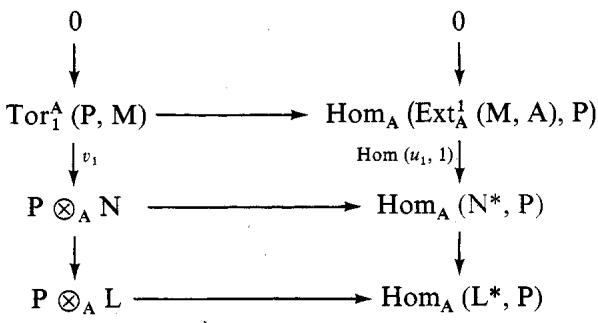
\includegraphics[keepaspectratio]{images/part001_66a54857.jpg}}

其中各列是正合的；在这种情况下我们推出结论。若 \(n \geqslant 2\) ，映射 \(u_n\) 与 \(v_n\) 是双射的（X，第 128 页，推论 4 及第 131 页，推论 3）。由归纳假设，典范同态

\[
\operatorname{Tor} _ {n - 1} ^ {\mathbf {A}} (\mathrm{P}, \mathrm{N}) \rightarrow \operatorname{Hom} _ {\mathbf {A}} \left(\operatorname{Ext} _ {\mathbf {A}} ^ {n - 1} (\mathrm{N}, \mathrm{A}), \mathrm{P}\right)
\]

是单射（相应地，双射）；图表（5）表明典范同态 \(\mathrm{Tor}_{n}^{\mathrm{A}}(\mathrm{P},\mathrm{M})\to \mathrm{Hom}_{\mathrm{A}}(\mathrm{Ext}_{\mathrm{A}}^{n}(\mathrm{M},\mathrm{A}),\mathrm{P})\) 也具有同样的性质，这完成了证明。

\subsection{环的同调维数}

定义 2. --- 称 A 的同调维数，并记作 dh(A)，其为 \(\overline{\mathbf{Z}}\) 中整数 \(n\) （存在两个 A-模 M 与 N 满足 \(\operatorname{Ext}_{\mathbf{A}}^{n}(\mathbf{M},\mathbf{N})\neq0\) ）所成集合的上确界 .

我们有 \(\mathrm{dh}(0) = -\infty\) , \(\mathrm{dh(A)} \geqslant 0\) （如果 \(A \neq 0\) ）。下面将看到 \(\mathrm{dh(A)} = 1\) （如果 \(A\) 是主理想环且不是域），并且，若 \(K\) 是一个交换域

\[
\mathrm{dh} (\mathrm{K} [ \mathrm{X} _ {1}, \dots , \mathrm{X} _ {n} ]) = n.
\]

命题 4. --- 设 n 为整数且 n ≥ 0。以下条件等价：(i) dh(A) ≤ n，

\begin{enumerate}
\def\labelenumi{(\roman{enumi})}
\setcounter{enumi}{1}
\tightlist
\item
  对每个 A-模 M，有 \(\mathrm{dp}_{\mathbf{A}}(\mathbf{M}) \leqslant n\) ,
\end{enumerate}

(ii') 对每个有限生成的 A-模 M，有 \(\mathrm{dp}_{\mathbf{A}}(\mathbf{M}) \leqslant n\) ,

\begin{enumerate}
\def\labelenumi{(\roman{enumi})}
\setcounter{enumi}{2}
\tightlist
\item
  对每个正合序列
\end{enumerate}

\[
0 \rightarrow \mathrm{K} \rightarrow \mathrm{P} _ {n - 1} \rightarrow \mathrm{P} _ {n - 2} \rightarrow \dots \rightarrow \mathrm{P} _ {0}
\]

其中 \(P_{i}\) 是投射的，K 是投射的，

\begin{enumerate}
\def\labelenumi{(\roman{enumi})}
\setcounter{enumi}{3}
\tightlist
\item
  对每个正合序列
\end{enumerate}

\[
\mathrm{I} ^ {0} \rightarrow \mathrm{I} ^ {1} \rightarrow \dots \rightarrow \mathrm{I} ^ {n - 1} \rightarrow \mathrm{N} \rightarrow 0
\]

其中 \(\mathrm{I}^{i}\) 都是内射的，N 是内射的，

\begin{enumerate}
\def\labelenumi{(\alph{enumi})}
\setcounter{enumi}{21}
\tightlist
\item
  每个 A-模都有长度不超过 n 的内射分解。
\end{enumerate}

条件 (i)、(ii) 和 (iii) 的等价性由命题 1 得出。我们显然有 (ii) \(\Rightarrow\) (ii')。因此，我们只需证明 (ii') \(\Rightarrow\) (iv) \(\Rightarrow\) (v) \(\Rightarrow\) (i)。

(ii') \(\Rightarrow\) (iv)：使用(iv)中的记号，设 K 为 \(\mathrm{I}^{0} \to \mathrm{I}^{1}\) 的核。根据 X，第 128 页，推论 4，对每个 A-模 M，我们有一个同构 \(\operatorname{Ext}_{\mathbf{A}}^{1}(\mathbf{M}, \mathbf{N}) \to \operatorname{Ext}_{\mathbf{A}}^{n+1}(\mathbf{M}, \mathbf{K})\) ；于是由(ii')可知，对每个有限生成的 A-模 M， \(\operatorname{Ext}_{\mathbf{A}}^{1}(\mathbf{M}, \mathbf{N})\) 都为零。根据 X，第 93 页，命题 11，这意味着 N 是内射的，从而得到(iv)。

\begin{enumerate}
\def\labelenumi{(\roman{enumi})}
\setcounter{enumi}{3}
\tightlist
\item
  \(\Rightarrow\) (v)：设 M 为一个 A-模。将(iv)应用于正合序列
\end{enumerate}

\[
0 \rightarrow \mathrm{M} \rightarrow \mathrm{I} ^ {0} (\mathrm{M}) \rightarrow \mathrm{I} ^ {1} (\mathrm{M}) \rightarrow \dots \rightarrow \mathrm{I} ^ {n - 1} (\mathrm{M}) \rightarrow \mathrm{K} ^ {n - 1} (\mathrm{M}) \rightarrow 0
\]

由 X，第 52 页，我们得出结论： \(\mathbf{K}^{n-1}(\mathbf{M})\) 是内射的，由此得 (v)。

\begin{enumerate}
\def\labelenumi{(\alph{enumi})}
\setcounter{enumi}{21}
\tightlist
\item
  \(\Rightarrow\) (i)：这由 X，第 100 页，定理 1 得出。
\end{enumerate}

注记. --- 1) 如果 \(\mathrm{dh}(\mathbf{A}) \leqslant n < +\infty\) ，则对每个 A-模 M 和每个右 A-模 P 有 \(\operatorname{Tor}_{n+1}^{\mathbf{A}}(\mathbf{P}, \mathbf{M}) = 0\) ，因为 \(\mathrm{dp}_{\mathbf{A}}(\mathbf{M}) \leqslant n\) （参见引理 1）。

\begin{enumerate}
\def\labelenumi{\arabic{enumi})}
\setcounter{enumi}{1}
\tightlist
\item
  为使 dh(A) 有限，必要且充分的是对每个非零 A-模 M，dp\_A(M) 均为有限。这确实由前述内容及 X，第 135 页，推论 1 得出。
\end{enumerate}

推论. --- 设 A 为左诺特环，并设 n 为整数 \textgreater{} 0. 以下条件等价：

\begin{enumerate}
\def\labelenumi{(\roman{enumi})}
\item
  \(\mathrm{dh(A)}\leqslant n,\)
\item
  对于每一对有限生成的 A-模 M 和 N，我们有 \(\operatorname{Ext}_{\mathbf{A}}^{n+1}(\mathbf{M}, \mathbf{N}) = 0\) ,
\item
  对每个有限生成的左 A-模 M 和每个有限生成的右 A-模 P，我们有 \(\operatorname{Tor}_{n+1}^{\mathbf{A}}(\mathbf{P},\mathbf{M}) = 0\) .
\end{enumerate}

这由命题 2 和 4 得出。

注记. --- 由(i)与(iii)的等价性，若 A 是右且左诺特的，则 dh(A) = dh(A°)。此等式在一般情况下不成立（X，第 204 页，习题 20）。

命题 5. --- 设 A 是左诺特的且具有有限同调维数，并令 \(\mathcal{C}_{0}\) (相应地， \(\mathcal{C}\) ) 为有限生成投射 A-模（相应地，有限生成 A-模）的同构类集合。则 Grothendieck 群的典范同态 \(\mathrm{K}(\mathcal{C}_{0}) \to \mathrm{K}(\mathcal{C})\) 是双射。

这由 X，第 137 页，推论得出。

\subsection{同调维数为0的环}

命题 6. --- 以下条件等价：

\begin{enumerate}
\def\labelenumi{(\roman{enumi})}
\item
  每个 A-模都是投射的，
\item
  每个 A-模都是内射的，
\item
  A 的每个理想都是内射模，
\item
  \(\mathrm{dh}(\mathbf{A})\leqslant 0,\)
\item
  A 是半单的，
\item
  A 是诺特的且每个 A-模都是平坦的，
\item
  每个 A-模复形都是分裂的，
\item
  每个 A-模正合列都是分裂的。
\end{enumerate}

由命题 4，我们有(i) \(\Leftrightarrow\) (ii) \(\Leftrightarrow\) (iv)；由命题 4 的推论 1，我们有(vi) \(\Rightarrow\) (iv)。由 X，第 35 页，例 4，我们有(i) \(\Rightarrow\) (vii)；由于(ii) \(\Rightarrow\) (iii)和(vii) \(\Rightarrow\) (viii)是平凡的，且由于(viii) \(\Rightarrow\) (i)由 II，第 39 页，命题 4 得出，因此只需证明(iii) \(\Rightarrow\) (v)和(v) \(\Rightarrow\) (vi)；最后一个断言由 VIII，第 5 节，第 1 号，命题 1 和 2 得出；最后，如果 A 的每个理想都是内射的，则它是 A 中的直和项，从而(iii) \(\Rightarrow\) (v)。

\subsection{同调维数为1的环}

命题 7. --- 下列条件是等价的：

\begin{enumerate}
\def\labelenumi{(\roman{enumi})}
\item
  \(\mathrm{dh}(\mathbf{A})\leqslant 1\)
\item
  投射模的每个子模都是投射的，
\end{enumerate}

(ii') A 的每个理想都是投射的，

\begin{enumerate}
\def\labelenumi{(\roman{enumi})}
\setcounter{enumi}{2}
\item
  内射 A-模的每个商都是内射的，
\item
  对每个投射复形 C，存在一个拟同构 \(\varphi : \mathbf{C} \to \mathbf{H}(\mathbf{C})\) 使得 \(\mathbf{H}(\varphi) = 1_{\mathbf{H}(\mathbf{C})}\) ,
\item
  对每个内射复形 C，存在一个拟同构 \(\psi : \mathrm{H}(\mathbf{C}) \to \mathbf{C}\) 使得 \(\mathrm{H}(\psi) = 1_{\mathrm{H}(\mathbf{C})}\) .
\item
  (i) \(\Leftrightarrow\) (ii) \(\Leftrightarrow\) (iii)：这由 X，第 138 页，命题 4 得出。
\item
  \(\Rightarrow\) (iv)：设 C 为投射复形。若(ii)成立，则 C 的子模 B(C) 是投射的，从而由 X，第 35 页，注 b) 得(iv)。
\item
  \(\Rightarrow\) (v)：设 C 为内射复形。若(iii)成立，则商 \(B_{n}(C)\) （\(C_{n+1}\) 的）对每个 \(n\) 都是内射的，从而由 X，第 35 页，注 a) 得(v)。
\item
  \(\Rightarrow\) (ii)：设 P 为投射 A-模，M 为 P 的子模， \(i: \mathbf{M} \to \mathbf{P}\) 为典范单射。设 \(p: \mathbf{L} \to \mathbf{M}\) 为自由模 L 到 M 上的满同态。考虑投射复形 C，使得 \(\mathbf{C}_1 = \mathbf{L}\) , \(\mathbf{C}_0 = \mathbf{P}\) , \(\mathbf{C}_i = 0\) （当 \(i \neq 0\) , \(1\)）， \(d_1 = i \circ p\) . 若(iv)满足，设 \(\varphi: \mathbf{C} \to \mathbf{H}(\mathbf{C})\) 为拟同构使得 \(\mathbf{H}(\varphi) = 1_{\mathbf{H}(\mathbf{C})}\) 。由于 \(\mathbf{H}_1(\mathbf{C}) = \operatorname{Ker} p\) , \(\varphi_1\) 是 L 到 \(\operatorname{Ker} p\) 上的投影算子，正合序列
\end{enumerate}

\[
0 \rightarrow \operatorname{Ker} p \rightarrow \mathrm{L} \xrightarrow {p} \mathrm{M} \rightarrow 0
\]

是分裂的，且 M 同构于 L 的一个直和项，因此是投射的。

\begin{enumerate}
\def\labelenumi{(\alph{enumi})}
\setcounter{enumi}{21}
\tightlist
\item
  \(\Rightarrow\) (iii)：设 I 为内射模，M 为 I 的商， \(\pi : \mathrm{I} \to \mathrm{M}\) 为典范投影。设 \(i: \mathrm{M} \to \mathrm{J}\) 为 M 到内射模 J 内的单同态。考虑内射复形 C，使得 \(C^0 = I\) , \(C^1 = J\) , \(C^i = 0\) （当 \(i \neq 0, 1\)）， \(d^0 = i \circ \pi\) 。若(v)满足，设 \(\psi : \mathrm{H}(\mathbf{C}) \to \mathbf{C}\) 为拟同构使得 \(\mathrm{H}(\psi) = 1_{\mathrm{H}(\mathbf{C})}\) 。由于
\end{enumerate}

\[
\mathrm{H} ^ {1} (\mathrm{C}) = \text { Coker } i  ,
\]

\(\psi^{1}\) 是典范投影 J → Coker i 的一个截面，且 M 是 J 的一个直和项，因此是内射的。

\begin{enumerate}
\def\labelenumi{(\roman{enumi})}
\setcounter{enumi}{1}
\tightlist
\item
  \(\Rightarrow\) (ii')：这是平凡的。
\end{enumerate}

(ii') \(\Rightarrow\) (ii)：这由 VII，第 3 节，定理 1 的推论 1 得出。

例. --- 若 A 是主理想环，则 dh(A) ≤ 1。

注. --- 若 A 是（交换）整环，则前述条件也等价于：

满足这些条件的整环称为戴德金环（参见 X，第 204 页，习题 12 以及 AC，VII，第 2 节，第 2 号，定理 1）。

推论. --- 设 A 为同调维数 ≤ 1 的环，C 为投射 A-模的复形， \(\tilde{C}\) 为投射右 A-模的复形，C' 为内射 A-模的复形，P 为右 A-模，M 为左 A-模，n 为整数。则我们有分裂正合序列

\[
\begin{array}{r l} & 0 \to \bigoplus_ {p + q = n} \mathrm{H} _ {p} (\tilde {\mathrm{C}}) \otimes_ {\mathrm{A}} \mathrm{H} _ {q} (\mathrm{C}) \xrightarrow {\gamma} \mathrm{H} _ {n} (\tilde {\mathrm{C}} \otimes_ {\mathrm{A}} \mathrm{C}) \xrightarrow {\alpha} \bigoplus_ {p + q = n - 1} \mathrm{Tor} _ {1} ^ {\mathrm{A}} \left(\mathrm{H} _ {p} (\tilde {\mathrm{C}}), \mathrm{H} _ {q} (\mathrm{C})\right) \to 0, \\ & 0 \to \prod_ {p} \mathrm{Ext} _ {\mathrm{A}} ^ {1} \left(\mathrm{H} _ {p} (\mathrm{C}), \mathrm{H} ^ {n - p - 1} (\mathrm{C} ^ {\prime})\right) \xrightarrow {\beta} \mathrm{H} ^ {n} (\mathrm{Homgr} _ {\mathrm{A}} (\mathrm{C}, \mathrm{C} ^ {\prime})) \\ & \qquad \qquad \qquad \xrightarrow {\lambda_ {p}} \prod_ {p} \mathrm{Homgr} _ {\mathrm{A}} \left(\mathrm{H} _ {p} (\mathrm{C}), \mathrm{H} ^ {n - p} (\mathrm{C} ^ {\prime})\right) \to 0, \\ & 0 \to \mathrm{P} \otimes_ {\mathrm{A}} \mathrm{H} _ {n} (\mathrm{C}) \xrightarrow {\gamma_ {p}} \mathrm{H} _ {n} (\mathrm{P} \otimes_ {\mathrm{A}} \mathrm{C}) \xrightarrow {\alpha_ {p}} \mathrm{Tor} _ {1} ^ {\mathrm{A}} \left(\mathrm{P}, \mathrm{H} _ {n - 1} (\mathrm{C})\right) \to 0, \\ & 0 \to \mathrm{Ext} _ {\mathrm{A}} ^ {1} \left(\mathrm{H} _ {n - 1} (\mathrm{C}), \mathrm{M}\right) \xrightarrow {\beta_ {p}} \mathrm{H} ^ {n} (\mathrm{Homgr} _ {\mathrm{A}} (\mathrm{C}, \mathrm{M})) \xrightarrow {\lambda_ {p}} \mathrm{Hom} _ {\mathrm{A}} \left(\mathrm{H} _ {n} (\mathrm{C}), \mathrm{M}\right) \to 0. \end{array}
\]

由于 \(Z(C)\) , \(B(C)\) , \(Z(\tilde{C})\) 与 \(B(\tilde{C})\) 是投射的且 \(B(C')\) 是内射的，这由 \(X\) ，第 78 页，推论 2，第 96 页，推论 1 和第 98 页，推论 2 得出。

\subsection{多项式环的同调维数}

引理 2. --- 设 \(\rho: \mathbf{A} \to \mathbf{A}'\) 为环同态，M 为 A-模， \(\mathbf{M}'\) 为 \(\mathbf{A}'\) -模。若 A-模 \(\mathbf{A}_d'\) 是平坦的，则我们有 \(\mathrm{dp}_{\mathbf{A}'}(\mathbf{A}' \otimes_{\mathbf{A}} \mathbf{M}) \leqslant \mathrm{dp}_{\mathbf{A}}(\mathbf{M})\) 。若 A-模 \(\mathbf{A}_s'\) 是投射的，则我们有 \(\mathrm{dp}_{\mathbf{A}}(\mathbf{M}') \leqslant \mathrm{dp}_{\mathbf{A}'}(\mathbf{M}')\) .

第一个断言在 \(\mathrm{dp}_{\mathbf{A}}(\mathbf{M}) = \pm \infty\) 时是显然的；若 \(\mathrm{dp}_{\mathbf{A}}(\mathbf{M}) = n \in \mathbb{N}\) ，则存在 A-模的正合序列

\[
0 \rightarrow \mathrm{P} _ {n} \rightarrow \mathrm{P} _ {n - 1} \rightarrow \dots \rightarrow \mathrm{P} _ {0} \rightarrow \mathrm{M} \rightarrow 0
\]

其中 \(P_{i}\) 是投射的；A'-模的序列

\[
0 \rightarrow \mathrm{A} ^ {\prime} \otimes_ {\mathrm{A}} \mathrm{P} _ {n} \rightarrow \mathrm{A} ^ {\prime} \otimes_ {\mathrm{A}} \mathrm{P} _ {n - 1} \rightarrow \dots \rightarrow \mathrm{A} ^ {\prime} \otimes_ {\mathrm{A}} \mathrm{P} _ {0} \rightarrow \mathrm{A} ^ {\prime} \otimes_ {\mathrm{A}} \mathrm{M} \rightarrow 0
\]

是正合的，因为 \(\mathbf{A}_d'\) 是平坦的，且 \(\mathbf{A}'\) -模 \(\mathbf{A}' \otimes_{\mathbf{A}} \mathrm{P}_i\) 是投射的（II，第 89 页，推论）；因此 \(\mathrm{dp}_{\mathbf{A}'}(\mathbf{A}' \otimes_{\mathbf{A}} \mathbf{M}) \leqslant n = \mathrm{dp}_{\mathbf{A}}(\mathbf{M})\) 。第二个断言在 \(\mathrm{dp}_{\mathbf{A}'}(\mathbf{M}') = \pm \infty\) 时是显然的；若 \(\mathrm{dp}_{\mathbf{A}'}(\mathbf{M}') = m \in \mathbf{N}\) ，则存在 \(\mathbf{A}'\) -模的一个正合序列

\[
0 \to \mathrm{P} _ {m} ^ {\prime} \to \mathrm{P} _ {m - 1} ^ {\prime} \to \dots \to \mathrm{P} _ {0} ^ {\prime} \to \mathrm{M} ^ {\prime} \to 0,
\]

其中 \(P_{i}^{\prime}\) 是投射的；底层的 A-模序列是正合的。另一方面，每个 \(P_{i}^{\prime}\) 是某个模 \(A_{s}^{\prime(I)}\) 的 A'-子模的一个直和项，因此是投射的 A-模；所以我们有 \(\mathrm{dp}_{\mathbf{A}}(\mathbf{M}^{\prime}) \leqslant m = \mathrm{dp}_{\mathbf{A}^{\prime}}(\mathbf{M}^{\prime})\) .

引理 3. --- 设 A 是交换的，并令 M 为一个 A{[}X{]}-模。

\begin{enumerate}
\def\labelenumi{\alph{enumi})}
\item
  我们有 \(\mathrm{dp}_{\mathbf{A}}(\mathbf{M}) \leqslant \mathrm{dp}_{\mathbf{A}[\mathbf{X}]}(\mathbf{M}) \leqslant \mathrm{dp}_{\mathbf{A}}(\mathbf{M}) + 1\) .
\item
  如果位似 \(X_{M}\) 是单射的，我们有 dp \(_{A}\) (M/XM) ≤ dp \(_{A[X]}\) (M)。
\item
  若 \(\mathbf{XM} = 0\) ，我们有 \(\mathrm{dp}_{\mathbf{A}}(\mathbf{M}) + 1 = \mathrm{dp}_{\mathbf{A}[\mathbf{X}]}(\mathbf{M}).\)
\item
  我们有一个 A{[}X{]}-模的正合序列（III，第 106 页及 VII，第 5 节，第 1 号）
\end{enumerate}

\[
0 \rightarrow \mathrm{A} [ \mathrm{X} ] \otimes_ {\mathrm{A}} \mathrm{M} \rightarrow \mathrm{A} [ \mathrm{X} ] \otimes_ {\mathrm{A}} \mathrm{M} \rightarrow \mathrm{M} \rightarrow 0;
\]

断言 (a) 由 X，第 135 页，推论 2 及引理 2 得出。

\begin{enumerate}
\def\labelenumi{\alph{enumi})}
\setcounter{enumi}{1}
\tightlist
\item
  若 \(\mathrm{dp}_{\mathbf{A}[\mathbf{X}]}(\mathbf{M}) = \pm \infty\) 该断言是平凡的。如果 \(\mathbf{M}\) 是投射的且非零，则 A-模 \(\mathbf{M} / \mathbf{XM}\) 等同于 \(\mathbf{A} \otimes_{\mathbf{A}[\mathbf{X}]} \mathbf{M}\) ，因此是投射的，并且我们有 \(\mathrm{dp}_{\mathbf{A}}(\mathbf{M} / \mathbf{XM}) \leqslant 0 = \mathrm{dp}_{\mathbf{A}[\mathbf{X}]}(\mathbf{M})\) 。让我们对 \(\mathrm{dp}_{\mathbf{A}[\mathbf{X}]}(\mathbf{M}) = n\) （假设其 \(>0\) ）进行归纳推理。考虑 \(\mathbf{A}[\mathbf{X}]\) -模的一个正合序列 \(0 \to \mathbf{N} \to \mathbf{L} \to \mathbf{M} \to 0\) ，其中 \(\mathbf{L}\) 是一个自由 \(\mathbf{A}[\mathbf{X}]\) -模；将该图表应用于
\end{enumerate}

\[
\begin{array}{c} 0 \longrightarrow \mathrm{N} \longrightarrow \mathrm{L} \longrightarrow \mathrm{M} \longrightarrow 0 \\ \mathrm {X_ {N}} \Big \downarrow \quad \mathrm {X_ {L}} \Big \downarrow \quad \mathrm {X_ {M}} \Big \downarrow \\ 0 \longrightarrow \mathrm{N} \longrightarrow \mathrm{L} \longrightarrow \mathrm{M} \longrightarrow 0 \end{array}
\]

将 X，第 4 页的命题 2 应用于该图表，我们看到 \(X_{N}\) 是单射的，并且我们有正合序列

\[
0 \rightarrow \mathrm{N} / \mathrm{XN} \rightarrow \mathrm{L} / \mathrm{XL} \rightarrow \mathrm{M} / \mathrm{XM} \rightarrow 0.
\]

由于 L 在 A{[}X{]} 上是自由的，L/XL 在 A 上是自由的，且我们有

\[
\mathrm{dp} _ {\mathbf {A} [ \mathbf {X} ]} (\mathbf {N}) = n - 1, \quad \mathrm{dp} _ {\mathbf {A}} (\mathbf {M} / \mathbf {X M}) \leqslant 1 + \mathrm{dp} _ {\mathbf {A}} (\mathbf {N} / \mathbf {X N});
\]

由于由归纳假设 dp \(_{A}\) (N/XN) ≤ n - 1 ，我们推出 dp \(_{A}\) (M/XM) ≤ n，这正是所要证明的。

\begin{enumerate}
\def\labelenumi{\alph{enumi})}
\setcounter{enumi}{2}
\tightlist
\item
  该断言在 \(\mathrm{dp}_{\mathbf{A}[\mathbf{X}]}(\mathbf{M}) = \pm \infty\) 时是平凡的，并且在 \(\mathrm{dp}_{\mathbf{A}[\mathbf{X}]}(\mathbf{M}) = 0\) 时也是平凡的（这是不可能的，因为 \(\mathbf{XM} = 0\) ）。因此我们可以假设 \(\mathrm{dp}_{\mathbf{A}[\mathbf{X}]}(\mathbf{M}) = n > 0\) 。如上考虑一个正合序列 \(0 \to \mathbf{N} \to \mathbf{L} \to \mathbf{M} \to 0\) ，其中 \(\mathbf{L}\) 是一个自由 \(\mathbf{A}[\mathbf{X}]\) -模，我们得到 \(\mathbf{A}\) -模的一个正合序列
\end{enumerate}

\[
0 \rightarrow \mathrm{M} \rightarrow \mathrm{N} / \mathrm{XN} \rightarrow \mathrm{L} / \mathrm{XL} \rightarrow \mathrm{M} \rightarrow 0.
\]

由 b)，我们有 \(\mathrm{dp}_{\mathbf{A}}(\mathbf{N} / \mathbf{X}\mathbf{N}) \leqslant \mathrm{dp}_{\mathbf{A}[\mathbf{X}]}(\mathbf{N}) = \mathrm{dp}_{\mathbf{A}[\mathbf{X}]}(\mathbf{M}) - 1 = n - 1\) ；由于 \(\mathrm{dp}_{\mathbf{A}}(\mathbf{L} / \mathbf{XL}) = 0\) ，从前面的正合序列出发，应用 X，第 135 页，推论 2 两次，我们推出 \(\mathrm{dp}_{\mathbf{A}}(\mathbf{M}) \leqslant n - 1\) 。但由 a)，我们有

\[
\mathrm{dp} _ {\mathbf {A}} (\mathbf {M}) \geqslant \mathrm{dp} _ {\mathbf {A} [ \mathbf {X} ]} (\mathbf {M}) - 1 = n - 1,
\]

由此得 c)。

定理 1. --- 设 A 是交换的。则

\[
\mathrm{dh} (\mathbf {A} [ \mathbf {X} ]) = \mathrm{dh} (\mathbf {A}) + 1.
\]

对每个 A{[}X{]}-模 M，我们有（引理 3）

\[
\mathrm{dp} _ {\mathbf {A} [ \mathbf {X} ]} (\mathbf {M}) \leqslant \mathrm{dp} _ {\mathbf {A}} (\mathbf {M}) + 1 \leqslant \mathrm{dh} (\mathbf {A}) + 1
\]

因此 \(\mathrm{dh}(\mathbf{A}[\mathbf{X}]) \leqslant \mathrm{dh}(\mathbf{A}) + 1\) ；反之，若 \(\mathbf{M}\) 是一个 A-模，令 \(\overline{\mathbf{M}}\) 为 \(\mathbf{A}[\mathbf{X}]\) -模，它由赋予 \(\mathbf{M}\) 使 \(\mathbf{X}\mathbf{M} = 0\) 的结构而得到，则（引理 3）

\[
\mathrm{d} p _ {\mathrm{A}} (\mathrm{M}) = \mathrm{d} p _ {\mathrm{A} [ \mathrm{X} ]} (\overline {{\mathrm{M}}}) - 1 \leqslant \mathrm{d} h (\mathrm{A} [ \mathrm{X} ]) - 1,
\]

因此 dh(A) ≤ dh(A{[}X{]}) - 1.

推论 1. --- 设 A 是交换的。我们有

\[
\mathrm{dh} (\mathrm{A} [ \mathrm{X} _ {1}, \dots , \mathrm{X} _ {n} ]) = \mathrm{dh} (\mathrm{A}) + n.
\]

这由定理对 n 进行归纳得出。

推论 2. --- 设 K 是一个交换域（相应地，一个主理想环* 或一个非域的戴德金环*）。则 dh(K{[}X₁, \ldots, Xₙ{]}) 等于 n（相应地，n + 1）。这由 dh(K) = 0（相应地，dh(K) = 1）这一事实得出。

\subsection{分次模的同调维数}

在本节中，我们假设 A 是次数 ≥ 0 的分次环。我们用 \((\mathbf{A}_{n})_{n \in \mathbf{Z}}\) 表示其分次结构；因此我们有 \(A_{n} = 0\) （对 n \textless{} 0）， \(A_{0}\) 是 A 的一个子环， \(J_{0} = \bigoplus_{n > 0} A_{n}\) 是 A 的一个双边理想，并且商分次环 \(A/J_{0}\) 等同于 \(A_{0}\) .

引理 4. --- 设 M 是一个下有界的分次 A-模（X，第 56 页）。如果 \(\mathbf{A}_0\otimes_{\mathbf{A}}\mathbf{M} = 0\) ，则 \(\mathbf{M} = 0\) .

由于 \(A_{0} \otimes_{A} M\) 同构于 \(M/J_{0} M\) ，这正是 II，第 171 页，命题 6。

引理 5. --- 设 M 是一个下有界的分次 A-模，并设

\[
s: \mathbf {A} \otimes_ {\mathbf {A} _ {0}} \mathrm{M} / \mathrm{J} _ {0} \mathrm{M} \rightarrow \mathrm{M}
\]

是一个分次 A-同态，使得 \(1 \otimes_{\mathbf{A}} s: \mathbf{A}_0 \otimes_{\mathbf{A}} (\mathbf{A} \otimes_{\mathbf{A}_0} \mathbf{M} / \mathrm{J}_0 \mathbf{M}) \to \mathbf{A}_0 \otimes_{\mathbf{A}} \mathbf{M}\) 是典范同构。则 s 是满射。若 \(\operatorname{Tor}_1^{\mathbf{A}}(\mathbf{A}_0, \mathbf{M}) = 0\) ，则 s 是双射。

我们有一个正合序列

\[
0 \rightarrow \operatorname{Ker} s \rightarrow A \otimes_ {A _ {0}} M / J _ {0} M \xrightarrow {s} M \rightarrow \operatorname{Coker} s \rightarrow 0
\]

且分次 A-模 Ker \(s\) 和 Coker \(s\) 是下有界的。由正合序列 \(\mathbf{A}_{0} \otimes_{\mathbf{A}} (\mathbf{A} \otimes_{\mathbf{A}_{0}} \mathrm{M} / \mathrm{J}_{0} \mathrm{M}) \xrightarrow{1 \otimes s} \mathbf{A}_{0} \otimes_{\mathbf{A}} \mathrm{M} \to \mathbf{A}_{0} \otimes_{\mathbf{A}} \text{Coker } s \to 0\) ，我们推出 \(\mathbf{A}_{0} \otimes_{\mathbf{A}} \text{Coker } s = 0\) ，因此 \(s\) 是满射（引理 4）。于是我们有一个正合序列

\[
\operatorname{Tor} _ {1} ^ {\mathrm{A}} \left(\mathrm{A} _ {0}, \mathrm{M}\right)\rightarrow \mathrm{A} _ {0} \otimes_ {\mathrm{A}} \operatorname{Ker} s \rightarrow \mathrm{A} _ {0} \otimes_ {\mathrm{A}} \left(\mathrm{A} \otimes_ {\mathrm{A} _ {0}} \mathrm{M} / \mathrm{J} _ {0} \mathrm{M}\right) \xrightarrow {1 \otimes s} \mathrm{A} _ {0} \otimes_ {\mathrm{A}} \mathrm{M}.
\]

若 \(\operatorname{Tor}_1^{\mathbf{A}}(\mathbf{A}_0, \mathbf{M}) = 0\) ，则 \(\mathbf{A}_0 \otimes_{\mathbf{A}} \operatorname{Ker} s = 0\) 且 \(s\) 是单射（引理 4）。

命题 8. --- 设 M 是一个下有界的分次 A-模。

\begin{enumerate}
\def\labelenumi{\alph{enumi})}
\tightlist
\item
  以下条件是等价的：
\end{enumerate}

\begin{enumerate}
\def\labelenumi{(\roman{enumi})}
\item
  M 同构于如下形式的分次 A-模： \(\mathbf{A} \otimes_{\mathbf{A}_0} \mathbf{N}\) ，其中 \(N\) 是分次投射（相应地，分次自由） \(\mathbf{A}_0\) -模；
\item
  M 是投射（相应地，自由）分次 A-模；
\item
  \(\mathbf{M} / \mathbf{J}_0\mathbf{M}\) 是投射（相应地，分次自由） \(\mathbf{A}_0\) -模，且 \(\operatorname{Tor}_1^{\mathbf{A}}(\mathbf{A}_0,\mathbf{M}) = 0\) .
\end{enumerate}

\begin{enumerate}
\def\labelenumi{\alph{enumi})}
\setcounter{enumi}{1}
\tightlist
\item
  进一步假设 M 有一个由有界次数的齐次元素组成的生成系。则以下条件等价：
\end{enumerate}

\begin{enumerate}
\def\labelenumi{(\roman{enumi})}
\item
  分次 A-模 M 具有一个有限合成列，其商同构于形如 \(A \otimes_{A_{0}} N\) 的分次 A-模，其中 N 是一个平坦分次 \(A_{0}\) -模；
\item
  M 是一个平坦 A-模；
\item
  \(\mathbf{M} / \mathrm{J}_0\mathbf{M}\) 是平坦 \(\mathbf{A}_0\) -模，且 \(\operatorname{Tor}_1^{\mathbf{A}}(\mathbf{A}_0,\mathbf{M}) = 0\) .
\end{enumerate}

在这两种情形中，我们显然有 (i) \(\Rightarrow\) (ii) \(\Rightarrow\) (iii). 因此我们必须证明 (iii) \(\Rightarrow\) (i).

\begin{enumerate}
\def\labelenumi{\alph{enumi})}
\tightlist
\item
  分次 A-模 A \(\otimes_{\mathbf{A}_0}\mathbf{M} / \mathbf{J}_0\) M 是投射 A-模，因为 \(\mathbf{M} / \mathbf{J}_0\) M 是投射 \(\mathbf{A}_0\) -模。A-模的典范同态
\end{enumerate}

\[
p: \mathbf {M} \rightarrow \mathbf {M} / \mathrm{J} _ {0} \mathbf {M}
\]

是满射；因此存在一个次数为 0 的分次 A-同态

\[
s: \mathbf {A} \otimes_ {\mathbf {A} _ {0}} \mathbf {M} / \mathrm{J} _ {0} \mathbf {M} \rightarrow \mathbf {M}
\]

使得 \(p \circ s(a \otimes x) = ax\) （对 \(a \in A\) 和 \(x \in M / J_0 M\) ）.

根据引理 5， \(s\) 是从 \(\mathbf{A} \otimes_{\mathbf{A}_0} \mathrm{M} / \mathrm{J}_0 \mathrm{M}\) 到 \(\mathbf{M}\) 上的 A-模同构，由此得 (i)。

\begin{enumerate}
\def\labelenumi{\alph{enumi})}
\setcounter{enumi}{1}
\tightlist
\item
  根据对 M 的假设，存在整数 a, b 使得 \(a \leqslant b\) 且 M 由 \(\oplus M_{i}\) 生成。让我们对正整数 b - a 进行归纳推理。
\end{enumerate}

若 \(b - a = 0\) 则 M 由 \(\mathbf{M}_a\) 生成，且典范 \(\mathbf{A}_0\) -同态 \(\mathbf{M}_a \to \mathbf{M} / \mathbf{J}_0\) M 是双射的；于是由 A-同态 \(\mathbf{A} \otimes_{\mathbf{A}_0} \mathbf{M}_a \to \mathbf{M}\) （由 M 作为 A-模的结构所定义）可推出一个分次 A-同态

\[
s: \mathbf {A} \otimes_ {\mathbf {A} _ {0}} \mathbf {M} / \mathrm{J} _ {0} \mathbf {M} \rightarrow \mathbf {M}
\]

满足引理 5 的条件。于是由引理 5，s 是双射的，从而 (i) 成立。

在一般情形中，设 \(\mathbf{M}^{(a)}\) 为 M 的由 \(M_{a}\) 生成的（分次）子 A-模，且设 \(M'\) 为商 \(\mathbf{M}/\mathbf{M}^{(a)}\) 。我们有一个正合序列

\[
0 \to \mathbf {M} ^ {(a)} \xrightarrow {f} \mathbf {M} \xrightarrow {g} \mathbf {M} ^ {\prime} \to 0,
\]

由此，由于根据假设 \(\mathrm{Tor}_{1}^{\mathbf{A}}(\mathbf{A}_{0},\mathbf{M}) = 0\) ，有正合序列

\begin{enumerate}
\def\labelenumi{(\arabic{enumi})}
\setcounter{enumi}{5}
\tightlist
\item
\end{enumerate}

\[
\begin{array}{c} \operatorname{Tor} _ {2} ^ {\mathsf {A}} (\mathbf {A} _ {0}, \mathbf {M} ^ {\prime}) \to \operatorname{Tor} _ {1} ^ {\mathsf {A}} (\mathbf {A} _ {0}, \mathbf {M} ^ {(a)}) \to 0 \\ 0 \to \operatorname{Tor} _ {1} ^ {\mathsf {A}} (\mathbf {A} _ {0}, \mathbf {M} ^ {\prime}) \to \operatorname{M} ^ {(a)} / \mathrm{J} _ {0} \operatorname{M} ^ {(a)} \xrightarrow {1 \otimes f} \operatorname{M} / \mathrm{J} _ {0} \operatorname{M} \xrightarrow {1 \otimes g} \operatorname{M} ^ {\prime} / \mathrm{J} _ {0} \operatorname{M} ^ {\prime} \to 0. \end{array}\tag{7}
\]

但典范同态 \(M_{a} \to M^{(a)}/J_{0} M^{(a)}\) 是双射的。由此可知同态 \(1 \otimes f : M^{(a)}/J_{0} M^{(a)} \to M/J_{0} M\) 是单射的，并且其像是 \(A_{0}\) -子模的、 \(M/J_{0} M\) 的一个直和项。由此，从正合序列 (7) 可得 \(\operatorname{Tor}_{1}^{A}(A_{0}, M') = 0\) ，且 \(A_{0}\) -模 \(M'/J_{0} M'\) 是平坦的，因为它同构于 \(M/J_{0} M\) 的一个直和项。根据归纳假设（该假设适用于 \(M'\) ，因为后者由 \(M'^{i}\) （\(a < i \leqslant b\) ）所生成）， \(M'\) 满足条件 (i)，因此是平坦的。于是从正合序列 (6) 可推出 \(\operatorname{Tor}_{1}^{A}(A_{0}, M^{(a)}) = 0\) ，而 \(M^{(a)}/J_{0} M^{(a)}\) 等同于 \(M_{a}\) ，后者是一个平坦的 \(A_{0}\) -模（作为 \(M/J_{0} M\) 的一个直和项子模）；根据已经证明的结果，分次 A-模 \(M^{(a)}\) 同构于 \(A \otimes_{A_{0}} M_{a}\) ，因此也满足 (i)，这完成了证明。

推论 1. --- 设 M 是一个有限生成的分次 A-模。如果 \(\mathbf{A}_0\) -模 \(\mathrm{M} / \mathrm{J}_0\) M 是投射的（相应地，分次自由的，相应地，平坦的），并且如果 \(\operatorname{Tor}_1^{\mathbf{A}}(\mathbf{A}_0, \mathbf{M}) = 0\) 则 A-模 M 是投射的（相应地，分次自由的，相应地，平坦的）。

推论 2. --- 假设每个投射 \(\mathbf{A}_{0}\) -模是自由的（相应地，设 A 是诺特的，且每个有限生成的投射 \(\mathbf{A}_{0}\) -模是自由的）。设 M 是一个下有界的分次 A-模（相应地，一个有限生成的分次 A-模），并设 n 为一个整数 \(\geqslant 0\) 使得 \(\mathrm{dp}_{\mathbf{A}}(\mathbf{M}) \leqslant n\) 。存在一个由分次 A-模与次数为 0 的分次同态构成的正合序列

\[
0 \rightarrow \mathrm{L} _ {n} \rightarrow \mathrm{L} _ {n - 1} \rightarrow \dots \rightarrow \mathrm{L} _ {0} \rightarrow \mathrm{M} \rightarrow 0
\]

其中 \(L_{i}\) 是分次自由的且有下界（相应地，分次自由且有限生成）。

事实上，存在（X，第 56 页，命题 11）一个由分次 A-模与 0 次同态构成的正合序列

\[
0 \to \mathrm{L} _ {n} \to \mathrm{L} _ {n - 1} \to \dots \to \mathrm{L} _ {0} \to \mathrm{M} \to 0
\]

其中 \(L_{i}\) 对 \(0 \leqslant i \leqslant n\) 是下方有界的（相应地，有限生成的），且对 \(0 \leqslant i \leqslant n - 1\) 是分次自由的 .

由于 \(\mathrm{dp}_{\mathbf{A}}(\mathbf{M}) \leqslant n\) ，A-模 \(L_{n}\) 是投射的；因此 \(\mathbf{A}_0 \otimes_{\mathbf{A}} L_n\) 是一个投射 \(\mathbf{A}_0\) -模，从而是分次自由的；由于 \(L_{n}\) 在下方有界且 \(\mathbf{A}_0 \otimes_{\mathbf{A}} L_n\) 分次自由， \(L_{n}\) 是分次自由的（命题 7）。

推论 3（希尔伯特合冲定理）. --- 假设 \(\mathbf{A}_0\) 是一个交换域，且 A 作为 \(\mathbf{A}_0\) -代数由 \(n\) 个次数 \(>0\) 的代数无关齐次元素生成。对于每个下方有界（相应地，有限型）的分次 A-模 M，存在一个由分次 A-模和次数为 0 的分次同态构成的正合序列

\[
0 \rightarrow L _ {n} \rightarrow L _ {n - 1} \rightarrow \dots \rightarrow L _ {0} \rightarrow M \rightarrow 0,
\]

其中 \(L_{i}\) 是分次自由的且有下界（相应地，且有限生成）。

事实上，由 X，第 143 页，定理 1 有 \(\mathrm{dh}(\mathbf{A}) = n\) ，并应用推论 2。

注记. --- 推论 2 也适用于以下情形：

\begin{enumerate}
\def\labelenumi{\alph{enumi})}
\item
  \(\mathbf{A}_0\) 是主理想环且 \(\mathbf{A} = \mathbf{A}_0[\mathbf{X}_1, \dots, \mathbf{X}_{n-1}]\) ;
\item
  * A \(_{0}\) 是维数为 r 的正则局部诺特环，且 A = A \(_{0}\) {[}X \(_{1}\) , \ldots，X \(_{n}\) ，r{]}. *
\end{enumerate}

推论 4. --- 假设 \(\mathbf{A}_{0}\) 半单。设 M 为有下界的分次 A-模，n 为整数 \(\geqslant 0\) 。对于 \(\mathrm{dp}_{\mathbf{A}}(\mathbf{M}) \leqslant n\) ，其充要条件是 \(\operatorname{Tor}_{n+1}^{\mathbf{A}}(\mathbf{A}_{0}, \mathbf{M}) = 0\) .

若 \(\mathrm{dp}_{\mathbf{A}}(\mathbf{M}) \leqslant n\) ，则 \(\operatorname{Tor}_{n+1}^{\mathbf{A}}(\mathbf{A}_0, \mathbf{M}) = 0\) （X，第 135 页，引理 1）。反之，设 \(0 \to \mathbf{K} \to \mathbf{L}_{n-1} \to \ldots \to \mathbf{L}_1 \to \mathbf{L}_0 \to \mathbf{M} \to 0\) 是下方有界的分次 A-模的正合序列，使得 \(\mathbf{L}_0, \ldots, \mathbf{L}_{n-1}\) 是分次自由的（X，第 56 页，命题 11）；由 X 第 131 页的推论 3，等式 \(\operatorname{Tor}_{n+1}^{\mathbf{A}}(\mathbf{A}_0, \mathbf{M}) = 0\) 蕴含 \(\operatorname{Tor}_1^{\mathbf{A}}(\mathbf{A}_0, \mathbf{K}) = 0\) ；由于 \(\mathbf{K} / \mathbf{J}_0\mathbf{K}\) 是一个投射 \(\mathbf{A}_0\) -模（因为 \(\mathbf{A}_0\) 是半单的；X，第 140 页，命题 6），K 由命题 8（X，第 144 页）是投射的，且 \(\mathrm{dp}_{\mathbf{A}}(\mathbf{M}) \leqslant n\) .

推论 5. --- 设环 \(\mathbf{A}_0\) 半单。若 \(\operatorname{Tor}_{n+1}^{\mathbf{A}}(\mathbf{A}_0, \mathbf{A}_0) = 0\) ，则我们有 \(\mathrm{dp}_{\mathbf{A}}(\mathbf{M}) \leqslant n\) （对每个下方有界的分次 \(\mathbf{A}\) -模）。

设 A° 表示 A 的反分次环：我们有 (A°)₀ = (A₀)°，因此 (A°)₀ 是半单的（VIII，§ 5，n° 1，注记 3）。由于 \(\operatorname{Tor}_{n+1}^{A°}(A₀°, A₀°) = 0\) ，由推论 4 有 \(\mathrm{dp}_A(A₀s) \leqslant n\) ：这意味着对每个 A-模 M 有 \(\operatorname{Tor}_{n+1}^{A°}(M₀, A₀°) = 0\) ，因此 \(\operatorname{Tor}_{n+1}^{A}(A₀, M) = 0\) ，我们应用推论 4。

\section{科斯居尔复形}

在本段中，所考虑的所有环都是交换环。
% semantic-fragments: legacy-input-seam
\relax{}
\subsection{\texorpdfstring{复形 \(\mathsf{K}(u),\mathsf{K}.(u,\mathsf{C}),\mathsf{K}^{\prime}(u,\mathsf{C})\)}{复形 \textbackslash mathsf\{K\}(u),\textbackslash mathsf\{K\}.(u,\textbackslash mathsf\{C\}),\textbackslash mathsf\{K\}\^{}\{\textbackslash prime\}(u,\textbackslash mathsf\{C\})}}

设 A 为环，L 为 A-模， \(u: \mathbf{L} \to \mathbf{A}\) 为线性形式，且 \(\Lambda(\mathbf{L})\) 为 A-模 L 的外代数。对于 \(x \in \Lambda(\mathbf{L})\) ，令 \(d_u(x)\) 表示内积 \(x \sqsubseteq u\) （III，第 161 页，例）。根据前引文第 162 页公式 (60)，我们有

\[
d _ {u} \left(e _ {1} \wedge \dots \wedge e _ {n}\right) = \sum_ {i = 1} ^ {n} (- 1) ^ {i + 1} u \left(e _ {i}\right) e _ {1} \wedge \dots \wedge e _ {i - 1} \wedge e _ {i + 1} \wedge \dots \wedge e _ {n}\tag{1}
\]

对 L 中的 \(e_1, \ldots, e_n\) 成立。根据 III，第 164 及 165 页，映射 \(d_u: \symbf{\Lambda}(\mathbf{L}) \to \symbf{\Lambda}(\mathbf{L})\) 是次数为 \((-1)\) 且平方为零的反导子。它是 A-代数 \(\symbf{\Lambda}(\mathbf{L})\) 中扩张 \(u: \symbf{\Lambda}^1(\mathbf{L}) \to \symbf{\Lambda}^0(\mathbf{L})\) 的唯一反导子。

定义 1.--- 复形 \((\symbf{\Lambda}(\mathbf{L}), d_u)\) 记作 \(\mathbf{K}^{\mathbf{A}}(u)\) 或 \(\mathbf{K}(u)\) 。

注意 \(\mathbf{K}_{n}(u)=\symbf{\Lambda}^{n}(\mathbf{L})=\mathbf{K}^{-n}(u)\) 。显然 \(\mathbf{K}(u)\) 右零，且 \(\mathrm{H}_{0}(\mathbf{K}(u))=\mathrm{Coker}(u)=\mathrm{A}/\mathfrak{q}\) ，其中 \(\mathfrak{q}\) 是 A 的理想 \(u(\mathbf{L})\) 。

对于 A-模的每个复形 C，我们设

\[
\mathbf {K} _ {\cdot} ^ {\mathrm{A}} (u, \mathrm{C}) = \mathrm{C} \otimes_ {\mathrm{A}} \mathbf {K} ^ {\mathrm{A}} (u), \quad \mathbf {K} _ {\cdot} ^ {\cdot} (u, \mathrm{C}) = \operatorname{Homgr} _ {\mathrm{A}} (\mathbf {K} ^ {\mathrm{A}} (u), \mathrm{C}).
\]

\[
\mathrm{H} ^ {\mathsf {A}} (u, \mathrm{C}) = \mathrm{H} (\mathrm{C} \otimes_ {\mathsf {A}} \mathbf {K} ^ {\mathsf {A}} (u)) \quad \mathrm{H} _ {\mathsf {A}} ^ {\bullet} (u, \mathrm{C}) = \mathrm{H} (\mathrm{Homgr} _ {\mathsf {A}} (\mathbf {K} ^ {\mathsf {A}} (u), \mathrm{C})) ,
\]

\[
\mathrm{H} _ {r} ^ {\mathrm{A}} (u, \mathrm{C}) = \mathrm{H} _ {r} (\mathrm{C} \otimes_ {\mathrm{A}} \mathbf {K} ^ {\mathrm{A}} (u)), \quad \mathrm{H} _ {\mathrm{A}} ^ {r} (u, \mathrm{C}) = \mathrm{H} ^ {r} (\operatorname{Homgr} _ {\mathrm{A}} (\mathbf {K} ^ {\mathrm{A}} (u), \mathrm{C})) .
\]

因此，我们有 A-模的典范同态（X，第 62 页及第 82 页）

\[
\gamma_ {0}: \mathrm{H} _ {0} (\mathbf {C}) \otimes_ {\mathbf {A}} \mathrm{A} / \mathfrak {q} \rightarrow \mathrm{H} _ {0} ^ {\mathbf {A}} (u, \mathbf {C}),
\]

\[
\lambda^ {0}: \mathrm{H} _ {\mathrm{A}} ^ {0} (u, \mathrm{C}) \rightarrow \operatorname{Hom} _ {\mathrm{A}} (\mathrm{A} / \mathfrak {q}, \mathrm{H} ^ {0} (\mathrm{C})).
\]

引理 1. --- 若复形 C 右零（相应地，左零），则 \(\mathbf{K}^{\mathbf{A}}(u,\mathbf{C})\) （相应地， \(\mathbf{K}_{\mathbf{A}}^{*}(u,c)\) ）右零（相应地，左零），并且 \(\gamma_{0}\) （相应地， \(\lambda^{0}\) ）是双射的。

这由 X，第 62 页，命题 1 及第 82 页，命题 1 得出。

命题 1. --- 设 \(x \in L\) ；记 \(\mathbf{R}_{x}: y \mapsto x \wedge y\) 为由 \(x\) 在代数 \(\boldsymbol{\Lambda}(\mathbf{L})\) 中左乘的映射。则有 \(d_{u} \circ \mathbf{R}_{x} + \mathbf{R}_{x} \circ d_{u} = u(x)\) . \(1_{\boldsymbol{\Lambda}(\mathbf{L})} = u(x)_{\boldsymbol{\Lambda}(\mathbf{L})}\) .

事实上， \((d_u \circ R_x + R_x \circ d_u)(y) = d_u(x \wedge y) + x \wedge d_u(y)\) ；由于 \(d_u\) 是一个导子， \(d_u(x \wedge y) + x \wedge d_u(y) = d_u(x) \wedge y = u(x).y\) .

推论 1. --- 若 u 是满射的，则 \(\mathbf{K}(u)\) 同伦于零（X，第 34 页）， \(\mathbf{K}_{\cdot}^{\mathrm{A}}(u,\mathrm{C})\) 和 \(\mathbf{K}_{\cdot}^{\cdot}(\mathbf{u},\mathbf{C})\) 对每个复形 C 也如此。

事实上，存在 \(x \in \mathbf{L}\) 使得 \(u(x) = 1\) 。于是 \(\mathbf{K}(u)\) 由命题 1 同伦于零，因而 \(\mathbf{K}^{\mathrm{A}}(u, \mathbf{C})\) （X，第 64 页，命题 3）与 \(\mathbf{K}_{\mathrm{A}}^{*}(u, \mathbf{C})\) （X，第 83 页，命题 3）也如此。

推论 2. --- 设 C 是一个复形，Ann(C) 为其零化子。则 q + Ann(C) 零化 H \(^{A}\) (u, C) 与 H \(^{*}_{A}\) (u, C)。

对每个 \(\lambda \in q\) ，位似 \(\lambda_{\mathbf{K}(u)}\) 由该命题同伦于零，因此 \(1_{C} \otimes \lambda_{\mathbf{K}(u)}\) 以及 Homgr \((\lambda_{\mathbf{K}(u)}, 1_{C})\) 依据 X，第 64 页，命题 3 及 X，第 83 页，命题 3 也同伦于零；由此可知 \(\lambda\) 零化 H.(u, C) 与 H'(u, C)。若 \(\lambda \in \text{Ann}(C)\) ，则 \(1_{\mathbf{K}(u)} \otimes \lambda_{C}\) 以及 Homgr \((1_{\mathbf{K}(u)}, \lambda_{C})\) 为零。

假设 L 是投射的（相应地， \(\mathbf{K}(u)\) 在次数 \(>0\) 时零调）。则复形 \(\symbf{\Lambda}(\mathbf{L})\) 是投射的（相应地，是 A/q 的一个分解），依据 III，第 87 页，推论 2；由 X，第 102 页（相应地，第 100 页），因此对每个 A-模 M，我们有同态

\begin{enumerate}
\def\labelenumi{(\arabic{enumi})}
\setcounter{enumi}{1}
\tightlist
\item
\end{enumerate}

\[
\mathrm{H} _ {r} ^ {\mathbf {A}} (u, \mathrm{M}) \rightarrow \operatorname{Tor} _ {r} ^ {\mathbf {A}} (\mathrm{A} / \mathrm{q}, \mathrm{M}), \quad \operatorname{Ext} _ {\mathbf {A}} ^ {r} (\mathrm{A} / \mathrm{q}, \mathrm{M}) \rightarrow \mathrm{H} _ {\mathbf {A}} ^ {r} (u, \mathrm{M})\tag{3}
\]

\[
\operatorname{Tor} _ {r} ^ {\mathrm{A}} (\mathrm{A} / \mathrm{q}, \mathrm{M}) \rightarrow \mathrm{H} _ {r} ^ {\mathrm{A}} (u, \mathrm{M}), \quad \mathrm{H} ^ {r} (u, \mathrm{M}) \rightarrow \operatorname{Ext} _ {\mathrm{A}} ^ {r} (\mathrm{A} / \mathrm{q}, \mathrm{M}).
\]

若 L 是投射的且 \(\mathbf{K}(u)\) 在次数 \(>0\) 时零调，则上述同态 (2) 和 (3) 是双射且互为逆（X，第 102 页，命题 1）。

命题 2. --- 设 \((\mathbf{L}_{i})_{i\in I}\) 为一族 A-模，其中集合 I 有限且全序。设 u 为 \(\bigoplus_{i\in I}\mathbf{L}_{i}\) 上的线性形式， \(u_{i}\) 为它在 \(\mathbf{L}_{i}\) 上的限制。

A-代数的典范同构（III，第 84 页）

\[
g: \bigotimes_{\substack{i\in I}}\symbf{\Lambda}(\mathrm{L}_{i})\to \symbf{\Lambda}(\bigoplus_{i\in I}\mathrm{L}_{i})
\]

是复形 \(\otimes \mathbf{K}(u_i)\) （X，第 63 页）到复形 \(\mathbf{K}(u)\) 上的同构。

事实上，根据 X，第 64 页，注记 4，复形 \(\otimes_{i\in I}\mathbf{K}(u_i)\) 的微分 D 是一个反导子；反导子 \(d_u\) 与 \(g\circ D\circ g^{-1}\) （ \(\boldsymbol{\Lambda}(\oplus L_i)\) 的）在 \(\oplus L_i\) 上与映射 \(x\mapsto u(x)\) . 1（从 \(\oplus L_i\) 到 \(\boldsymbol{\Lambda}(\oplus L_i)\) ）一致，因此它们相等（III，第 128 页，推论）。

设 C 和 C' 是两个 A-模复形。我们有（X，第 63 页及第 99 页）复形的典范同构

\[
\mathbf {C} \otimes_ {\mathbf {A}} \left(\mathbf {C} ^ {\prime} \otimes_ {\mathbf {A}} \mathbf {K} (u)\right)\rightarrow \left(\mathbf {C} \otimes_ {\mathbf {A}} \mathbf {C} ^ {\prime}\right) \otimes_ {\mathbf {A}} \mathbf {K} (u)
\]

\[
\operatorname{Homgr} _ {\mathbf {A}} \left(\mathrm{C} ^ {\prime}, \operatorname{Homgr} _ {\mathbf {A}} (\mathbf {K} (u), \mathrm{C})\right)\rightarrow \operatorname{Homgr} _ {\mathbf {A}} \left(\mathrm{C} ^ {\prime} \otimes_ {\mathbf {A}} \mathbf {K} (u), \mathrm{C}\right),
\]

即，同构

\begin{enumerate}
\def\labelenumi{(\arabic{enumi})}
\setcounter{enumi}{3}
\tightlist
\item
\end{enumerate}

\[
\mathbf {C} \otimes_ {\mathbf {A}} \mathbf {K} ^ {\mathrm{A}} (u, \mathbf {C} ^ {\prime}) \rightarrow \mathbf {K} ^ {\mathrm{A}} (u, \mathbf {C} \otimes_ {\mathbf {A}} \mathbf {C} ^ {\prime})\tag{5}
\]

\[
\operatorname{Homgr} _ {\mathbf {A}} \left(\mathrm{C} ^ {\prime}, \mathbb {K} _ {\mathbf {A}} ^ {*} (u, \mathrm{C})\right)\rightarrow \operatorname{Homgr} _ {\mathbf {A}} \left(\mathbb {K} _ {\mathbf {A}} ^ {*} (u, \mathrm{C} ^ {\prime}), \mathrm{C}\right).
\]

在 (4) 和 (5) 中，取 \(\mathbf{C}^{\prime} = \mathbf{K}(u^{\prime})\) ，其中 \(u^{\prime}: L^{\prime} \to A\) 是 A-模 \(L^{\prime}\) 上的线性形式，并注意到 \(\mathbf{K}^{\mathrm{A}}(u, \mathbf{K}(u^{\prime}))\) 按定义等于 \(\mathbf{K}(u^{\prime}) \otimes_{\mathrm{A}} \mathbf{K}(u)\) ，根据命题 2，它等同于 \(\mathbf{K}(u^{\prime} \oplus u)\) ，其中 \(u^{\prime} \oplus u: L^{\prime} \oplus L \to A\) 是线性形式 \((x^{\prime}, x) \mapsto u^{\prime}(x^{\prime}) + u(x)\) 。于是我们得到复形的同构

\begin{enumerate}
\def\labelenumi{(\arabic{enumi})}
\setcounter{enumi}{5}
\tightlist
\item
\end{enumerate}

\[
\mathbf {K} _ {\bullet} ^ {\mathrm{A}} (u ^ {\prime} \oplus u, \mathrm{C}) \rightarrow \mathbf {K} _ {\bullet} ^ {\mathrm{A}} (u, \mathbf {K} _ {\bullet} ^ {\mathrm{A}} (u ^ {\prime}, \mathrm{C}))\tag{7}
\]

\[
\mathbf {K} _ {\mathrm{A}} ^ {\bullet} (u ^ {\prime}, \mathbf {K} _ {\mathrm{A}} ^ {\bullet} (u, \mathrm{C})) \rightarrow \mathbf {K} _ {\mathrm{A}} ^ {\bullet} (u ^ {\prime} \oplus u, \mathrm{C}).
\]

通过取同调，我们推出A-模的同构

\[
\begin{array}{c c} \mathrm{H} _ {r} ^ {\mathbf {A}} (u ^ {\prime} \oplus u, \mathrm{C}) \to \mathrm{H} _ {r} ^ {\mathbf {A}} (u, \mathbf {K} _ {\bullet} ^ {\mathbf {A}} (u ^ {\prime}, \mathrm{C}))  , & r \in \mathbf {Z}  , \\ \mathrm{H} _ {\mathbf {A}} ^ {r} (u ^ {\prime}, \mathbf {K} _ {\mathbf {A}} ^ {\bullet} (u, \mathrm{C})) \to \mathrm{H} _ {\mathbf {A}} ^ {r} (u ^ {\prime} \oplus u, \mathrm{C})  , & r \in \mathbf {Z}  . \end{array}
\]

最后，注意到由代数 \(\Lambda(L)\) 中的乘法导出的同态

\[
m: \mathbf {K} ^ {\mathrm{A}} (u) \otimes_ {\mathrm{A}} \mathbf {K} ^ {\mathrm{A}} (u) \rightarrow \mathbf {K} ^ {\mathrm{A}} (u)
\]

是复形态射（因为 \(d_{u}\) 是反导子）。假设 L 是秩为 \(n\) 的自由模，并与复形态射 \(\mathbf{K}^{\mathrm{A}}(u)\to\symbf{\Lambda}^{n}\mathrm{L}(-n)\) （它在次数 \(n\) 处为恒同）复合，由此导出一个复形态射

\[
\chi : \mathbf {K} ^ {\mathrm{A}} (u) \otimes_ {\mathrm{A}} \mathbf {K} ^ {\mathrm{A}} (u) \rightarrow \boldsymbol {\Lambda} ^ {n} \mathrm{L} (- n);
\]

根据 X，第 99 页，命题 12，该态射典范地对应一个复形态射

\[
\varphi : \mathbf {K} ^ {\mathrm{A}} (u) \rightarrow \operatorname{Homgr} _ {\mathrm{A}} \left(\mathbf {K} ^ {\mathrm{A}} (u), \boldsymbol {\Lambda} ^ {n} \mathrm{L} (- n)\right)
\]

它是双射的（III，第 87 页，公式 (20)）。对每个复形 C，由此导出一个复合同构

\[
\begin{array}{r l} \mathbf {K} _ {\bullet} ^ {\mathrm{A}} (u, \mathrm{C}) & = \mathrm{C} \otimes_ {\mathrm{A}} \mathbf {K} ^ {\mathrm{A}} (u) \xrightarrow {1 \otimes_ {\Phi}} \mathrm{C} \otimes \operatorname{Homgr} _ {\mathrm{A}} \left(\mathbf {K} ^ {\mathrm{A}} (u), \boldsymbol {\Lambda} ^ {n} \mathrm{L} (- n)\right) \to \\ & \to \operatorname{Homgr} _ {\mathrm{A}} \left(\mathbf {K} ^ {\mathrm{A}} (u), \mathrm{C} \otimes_ {\mathrm{A}} \boldsymbol {\Lambda} ^ {n} \mathrm{L} (- n)\right) = \mathbf {K} _ {\mathrm{A}} ^ {\bullet} (u, \mathrm{C} \otimes_ {\mathrm{A}} \boldsymbol {\Lambda} ^ {n} \mathrm{L} (- n)). \end{array}
\]

通过取同调，因此有典范同构

\[
\mathrm{H} _ {r} ^ {\mathbf {A}} (u, \mathrm{C}) \rightarrow \mathrm{H} _ {\mathbf {A}} ^ {n - r} (u, \mathrm{C} \otimes_ {\mathbf {A}} \boldsymbol {\Lambda} ^ {n} \mathrm{L}), \quad r \in \mathbf {Z}.\tag{8}
\]

注记。--- 1) * 当 L 为秩 n 的投射模时，前述结论仍然成立。~*

\begin{enumerate}
\def\labelenumi{\arabic{enumi})}
\setcounter{enumi}{1}
\tightlist
\item
  由于 L 是秩为 n 的自由模， \(\Lambda^{n}\) L 同构于 A，故有非典范同构 \(\mathrm{H}_{r}^{\mathrm{A}}(u,\mathrm{C})\to\mathrm{H}_{\mathrm{A}}^{n-r}(u,\mathrm{C})\) 。
\end{enumerate}

\subsection{函子性}

设 \(f: \mathbf{C} \to \mathbf{C}'\) 是复形的态射。我们用

\[
\begin{array}{l} \mathbf {K} _ {\bullet} ^ {\mathrm{A}} (u, f): \mathbf {K} _ {\bullet} ^ {\mathrm{A}} (u, \mathrm{C}) \to \mathbf {K} _ {\bullet} ^ {\mathrm{A}} (u, \mathrm{C} ^ {\prime}), \\ \mathbf {K} _ {\mathrm{A}} ^ {\bullet} (u, f): \mathbf {K} _ {\mathrm{A}} ^ {\bullet} (u, \mathrm{C}) \to \mathbf {K} _ {\mathrm{A}} ^ {\bullet} (u, \mathrm{C} ^ {\prime}), \end{array}
\]

表示复形的态射 \(f \otimes 1_{\mathbf{K}(u)}\) 和 \(\operatorname{Homgr}_{\mathbf{A}}(1_{\mathbf{K}(u)}, f)\) 。

我们用 \(\mathrm{H}_{\bullet}^{\mathrm{A}}(u,f):\mathrm{H}_{\bullet}^{\mathrm{A}}(u,\mathbf{C})\to\mathrm{H}_{\bullet}^{\mathrm{A}}(u,\mathbf{C}^{\prime}),\quad\mathrm{H}_{\mathrm{A}}^{\bullet}(u,f):\mathrm{H}_{\mathrm{A}}^{\bullet}(u,\mathbf{C})\to\mathrm{H}_{\mathrm{A}}^{\bullet}(u,\mathbf{C}^{\prime}),\quad\mathrm{H}_{r}^{\mathrm{A}}(u,f):\mathrm{H}_{r}^{\mathrm{A}}(u,\mathbf{C})\to\mathrm{H}_{r}^{\mathrm{A}}(u,\mathbf{C}^{\prime}),\mathrm{H}_{\mathrm{A}}^{r}(u,f):\mathrm{H}_{\mathrm{A}}^{r}(u,\mathbf{C})\to\mathrm{H}_{\mathrm{A}}^{r}(u,\mathbf{C}^{\prime})\) 表示在同调中诱导的态射。映射 \(f\mapsto\mathbf{K}_{\bullet}^{\mathrm{A}}(u,f)\) 是线性的；如果 \(g:\mathbf{C}^{\prime}\to\mathbf{C}^{\prime\prime}\) 是复形的另一个态射，我们有 \(\mathbf{K}_{\bullet}^{\mathrm{A}}(u,g\circ f)=\mathbf{K}_{\bullet}^{\mathrm{A}}(u,g)\circ\mathbf{K}_{\bullet}^{\mathrm{A}}(u,f)\) ；类似地，对于 \(\mathbf{K}_{\mathrm{A}}^{\bullet},\mathrm{H}_{\bullet}^{\mathrm{A}},\mathrm{H}_{\mathrm{A}}^{\bullet},\mathrm{H}_{r}^{\mathrm{A}},\mathrm{H}_{\mathrm{A}}^{r}\) .

设 \(0 \to \mathbf{C}' \xrightarrow{f} \mathbf{C} \xrightarrow{g} \dot{\mathbf{C}}'' \to 0\) 是复形的一个正合列。

\begin{enumerate}
\def\labelenumi{\alph{enumi})}
\tightlist
\item
  假设 L 是平坦的；则 \(\Lambda(L)\) 是平坦的（X，第 15 页，推论）。序列
\end{enumerate}

\[
0 \rightarrow \mathbf {K} _ {\bullet} ^ {\mathrm{A}} (u, C ^ {\prime}) \xrightarrow {\mathbf {K} _ {\bullet} ^ {\mathrm{A}} (u , f)} \mathbf {K} _ {\bullet} ^ {\mathrm{A}} (u, C) \xrightarrow {\mathbf {K} _ {\bullet} ^ {\mathrm{A}} (u , g)} \mathbf {K} _ {\bullet} ^ {\mathrm{A}} (u, C ^ {\prime \prime}) \rightarrow 0
\]

于是它是正合的，并（X，第 30 页）导出一个同调正合列。

\[
\dots \to \mathrm{H} _ {n} ^ {\mathbf {A}} (u, \mathrm{C} ^ {\prime}) \xrightarrow {\mathrm{H} _ {n} (u , f)} \mathrm{H} _ {n} ^ {\mathbf {A}} (u, \mathrm{C}) \xrightarrow {\mathrm{H} _ {n} (u , g)} \mathrm{H} _ {n} ^ {\mathbf {A}} (u, \mathrm{C} ^ {\prime \prime}) \xrightarrow {\hat {\sigma} _ {n}} \mathrm{H} _ {n - 1} ^ {\mathbf {A}} (u, \mathrm{C} ^ {\prime}) \to \dots .
\]

\begin{enumerate}
\def\labelenumi{\alph{enumi})}
\setcounter{enumi}{1}
\tightlist
\item
  假设 L 是投射的；则 \(\Lambda(L)\) 是投射的。序列
\end{enumerate}

\[
0 \rightarrow \mathbf {K} _ {\mathrm{A}} ^ {*} (u, \mathrm{C} ^ {\prime}) \xrightarrow {\mathbf {K} _ {\mathrm{A}} ^ {*} (u , f)} \mathbf {K} _ {\mathrm{A}} ^ {*} (u, \mathrm{C}) \xrightarrow {\mathbf {K} _ {\mathrm{A}} ^ {*} (u , g)} \mathbf {K} _ {\mathrm{A}} ^ {*} (u, \mathrm{C} ^ {\prime \prime}) \rightarrow 0
\]

于是它是正合的，并导出一个同调正合列。

\[
\dots \rightarrow \mathrm{H} _ {\mathrm{A}} ^ {n} (u, \mathrm{C} ^ {\prime}) \xrightarrow {\mathrm{H} ^ {n} (u , f)} \mathrm{H} _ {\mathrm{A}} ^ {n} (u, \mathrm{C}) \xrightarrow {\mathrm{H} ^ {n} (u , g)} \mathrm{H} _ {\mathrm{A}} ^ {n} (u, \mathrm{C} ^ {\prime \prime}) \xrightarrow {\partial^ {n}} \mathrm{H} _ {\mathrm{A}} ^ {n + 1} (u, \mathrm{C} ^ {\prime}) \rightarrow \dots .
\]

设 \(\rho: A \to A'\) 是一个环同态， \(L'\) 为 \(A'\) -模 \(A' \otimes_A L\) ， \(u': L' \to A'\) 为线性形式 \(1 \otimes u\) 。典范双射同态（III，第 83 页，命题 8）

\[
\psi : \Lambda_ {A ^ {\prime}} (A ^ {\prime} \otimes_ {A} L) \rightarrow A ^ {\prime} \otimes_ {A} \Lambda_ {A} (L)
\]

是 A'-模复形的同构。我们推出：

\begin{enumerate}
\def\labelenumi{\arabic{enumi})}
\tightlist
\item
  对每个 A'-模复形 C'，一个 A-模复形的同构
\end{enumerate}

\[
\mathbf {K} _ {\bullet} ^ {\mathrm{A} ^ {\prime}} \left(u ^ {\prime}, \mathrm{C} ^ {\prime}\right)\rightarrow \mathbf {K} _ {\bullet} ^ {\mathrm{A}} \left(u, \mathrm{C} ^ {\prime}\right),
\]

\begin{enumerate}
\def\labelenumi{(\arabic{enumi})}
\setcounter{enumi}{8}
\tightlist
\item
\end{enumerate}

它由图表

\[
\mathrm{C} ^ {\prime} \otimes_ {\mathrm{A} ^ {\prime}} \left(\boldsymbol {\Lambda} _ {\mathrm{A} ^ {\prime}} \left(\mathrm{A} ^ {\prime} \otimes_ {\mathrm{A}} \mathrm{L}\right)\right) \xrightarrow {1 _ {\mathrm{C} ^ {\prime}} \otimes \psi} \mathrm{C} ^ {\prime} \otimes_ {\mathrm{A} ^ {\prime}} \mathrm{A} ^ {\prime} \otimes_ {\mathrm{A}} \boldsymbol {\Lambda} _ {\mathrm{A}} (\mathrm{L}) \xrightarrow {\varphi} \mathrm{C} ^ {\prime} \otimes_ {\mathrm{A}} \boldsymbol {\Lambda} _ {\mathrm{A}} (\mathrm{L})
\]

复合而成，其中 φ 是典范双射（III，第 85 页，命题 14）；

\begin{enumerate}
\def\labelenumi{\arabic{enumi})}
\setcounter{enumi}{1}
\tightlist
\item
  对每个 A-模复形 C，一个 A'-模复形的同构
\end{enumerate}

\[
\mathbf {K} _ {\bullet} ^ {\mathrm{A}} (u, \mathrm{A} ^ {\prime} \otimes_ {\mathrm{A}} \mathrm{C}) \rightarrow \mathrm{A} ^ {\prime} \otimes_ {\mathrm{A}} \mathbf {K} _ {\bullet} ^ {\mathrm{A}} (u, \mathrm{C}),
\]

由此得到A'-模的同态

\[
\mathrm{A} ^ {\prime} \otimes_ {\mathrm{A}} \mathrm{H} _ {n} ^ {\mathrm{A}} (u, \mathrm{C}) \rightarrow \mathrm{H} _ {n} ^ {\mathrm{A} ^ {\prime}} (u ^ {\prime}, \mathrm{A} ^ {\prime} \otimes_ {\mathrm{A}} \mathrm{C}),
\]

当 A' 在 A 上平坦时，这些同态是双射的（X，第 66 页，推论 2）。

设 L' 为一个 A-模， \(u': L' \to A\) 为一个线性形式， \(f: L \to L'\) 为一个 A-同态，使得 \(u' \circ f = u\) 。由 III，第 161 页，公式 (55)，可知同态 \(\symbf{\Lambda}(f): \symbf{\Lambda}(\mathrm{L}) \to \symbf{\Lambda}(\mathrm{L}')\) 满足 \(d_u \circ \symbf{\Lambda}(f) = \symbf{\Lambda}(f) \circ d_{u'}\) ，从而定义了复形的态射 \(\symbf{\Lambda}(u): \mathbf{K}^{\mathbf{A}}(u) \to \mathbf{K}^{\mathbf{A}}(u')\) 。若 C 是一个 A-复形，我们推出复形的态射

\[
1 _ {C} \otimes \boldsymbol {\Lambda} (u): \mathbf {K} ^ {\mathrm{A}} (u, C) \rightarrow \mathbf {K} ^ {\mathrm{A}} \left(u ^ {\prime}, C\right) \quad \text { and }\quad \operatorname{Homgr} \left(\boldsymbol {\Lambda} (u), 1 _ {C}\right): \mathbf {K} _ {A} ^ {*} \left(u ^ {\prime}, C\right)\rightarrow \mathbf {K} _ {A} ^ {*} (u, C)
\]

若f是双射，则所有这些态射都是同构。

\subsection{\texorpdfstring{例1：复形 \(\mathbf{S}(\mathbf{L})\otimes_{\mathbf{A}}\boldsymbol{\Lambda}(\mathbf{L})\)}{例1：复形 \textbackslash mathbf\{S\}(\textbackslash mathbf\{L\})\textbackslash otimes\_\{\textbackslash mathbf\{A\}\}\textbackslash boldsymbol\{\textbackslash Lambda\}(\textbackslash mathbf\{L\})}}

设 A 为环，L 为 A-模， \(\mathbf{S}(\mathrm{L})\) 为其对称代数， \(\mathbf{S}(\mathrm{L}) \otimes_{\mathrm{A}} \mathrm{L}\) 为经纯量扩张得到的 \(\mathbf{S}(\mathrm{L})\) -模， \(u: \mathbf{S}(\mathrm{L}) \otimes_{\mathrm{A}} \mathrm{L} \to \mathbf{S}(\mathrm{L})\) 为线性形式，使得 \(u(s \otimes x) = sx\) 对 \(s \in \mathbf{S}(\mathrm{L})\) 、 \(x \in \mathrm{L}\) 成立。根据 \(\mathbf{S}(\mathrm{L})\) -模的典范同构（III，第 83 页，命题 8）

\[
\boldsymbol {\Lambda} _ {\mathbf {S} (L)} (\mathbf {S} (L) \otimes_ {A} L) \rightarrow \mathbf {S} (L) \otimes_ {A} \boldsymbol {\Lambda} (L),
\]

复形 \(\mathbf{K}^{\mathbf{S}(\mathrm{L})}(u)\) 的微分被搬运到映射

\[
d: \mathbf {S} (\mathrm{L}) \otimes_ {\mathrm{A}} \boldsymbol {\Lambda} (\mathrm{L}) \rightarrow \mathbf {S} (\mathrm{L}) \otimes_ {\mathrm{A}} \boldsymbol {\Lambda} (\mathrm{L})
\]

使得对 L 中的 \(x_{1},\ldots,x_{p},y_{1},\ldots,y_{q}\) ，我们有

\[
\begin{array}{l} d \left(\left(x _ {1} \dots x _ {p}\right) \otimes \left(y _ {1} \wedge \dots \wedge y _ {q}\right)\right) \\ = \sum_ {i = 1} ^ {q} (- 1) ^ {i + 1} y _ {i} x _ {1} \dots x _ {p} \otimes \left(y _ {1} \wedge \dots \wedge y _ {i - 1} \wedge y _ {i + 1} \wedge \dots \wedge y _ {q}\right). \end{array}
\]

注意 \(d\) 把 \(\mathbf{S}^{p}(\mathrm{L})\otimes\symbf{\Lambda}^{q}(\mathrm{L})\) 映到 \(\mathbf{S}^{p+1}(\mathrm{L})\otimes\symbf{\Lambda}^{q-1}(\mathrm{L})\) ，因此 A-模复形 \(\mathbf{S}(\mathrm{L})\otimes\symbf{\Lambda}(\mathrm{L})\) 分解为下述图表所描述的复形的直和：

\[
\left(\mathcal {E} _ {n}\right): 0 \rightarrow \mathbf {S} ^ {0} L \otimes_ {\mathrm{A}} \boldsymbol {\Lambda} ^ {n} L \rightarrow \mathbf {S} ^ {1} L \otimes_ {\mathrm{A}} \boldsymbol {\Lambda} ^ {n - 1} L \rightarrow \dots \rightarrow \mathbf {S} ^ {n} L \otimes_ {\mathrm{A}} \boldsymbol {\Lambda} ^ {0} L \rightarrow 0, n \in \mathbf {N}.
\]

若 A-模 L 是有限族 \((\mathbf{L}_{i})_{i\in I}\) 的直和，其中 I 是全序的，则典范双射

\[
\bigotimes_ {i \in I} ^ {\varepsilon} \left(\mathbf {S} (L _ {i}) \otimes_ {A} \boldsymbol {\Lambda} (L _ {i})\right) \to \mathbf {S} (L) \otimes_ {A} \boldsymbol {\Lambda} (L)
\]

是 A-模复形的同构（这由 X，第 148 页，命题 2 或上面的公式 (9) 推出）。

命题 3. --- 若 A-模 L 是平坦的，则上述序列 \((\mathcal{E}_n)\) 对 \(n > 0\) 是正合的。

\begin{enumerate}
\def\labelenumi{\alph{enumi})}
\tightlist
\item
  首先注意，若 \(p_{L}\) 是复合同态
\end{enumerate}

\[
\mathbf {S} (\mathrm{L}) \otimes \boldsymbol {\Lambda} (\mathrm{L}) \xrightarrow {\alpha} \mathbf {S} ^ {0} (\mathrm{L}) \otimes \boldsymbol {\Lambda} ^ {0} (\mathrm{L}) \xrightarrow {\beta} \mathrm{A},
\]

其中 \(\alpha\) 是诸典范投影的张量积， \(\beta\) 是典范同构；只需证明 \(\mathbf{H}(p_{\mathrm{L}})\) 是双射的。

\begin{enumerate}
\def\labelenumi{\alph{enumi})}
\setcounter{enumi}{1}
\item
  若L=0或L=A，命题显然成立。
\item
  假设 L 是有限秩的自由模；将它写成秩 1 的自由 A-模的直和 \(L_{1} \oplus \ldots \oplus L_{n}\) 。根据命题前的注记，复形 \(\mathbf{S}(\mathrm{L}) \otimes \symbf{\Lambda}(\mathrm{L})\) 同构于 n 个自由复形 \(\mathbf{S}(\mathrm{L}_{i}) \otimes \symbf{\Lambda}(\mathrm{L}_{i})\) 的张量积，后者的同调由 b) 知是自由的。由 X，第 79 页，推论 4，典范同态
\end{enumerate}

\[
\gamma : \bigoplus_ {i = 1} ^ {n} \mathrm{H} (\mathbf {S} (\mathrm{L} _ {i}) \otimes \boldsymbol {\Lambda} (\mathrm{L} _ {i})) \rightarrow \mathrm{H} (\mathbf {S} (\mathrm{L}) \otimes \boldsymbol {\Lambda} (\mathrm{L}))
\]

是双射的。由 b) 知 \(\mathrm{H}(p_{\mathrm{L}_i})\) 对所有 \(i\) 都是双射的。由于 \(\bigotimes_{i=1}^{n} \mathrm{H}(p_{\mathrm{L}_i}) = \mathrm{H}(p_{\mathrm{L}}) \circ \gamma\) ，

\[
\mathrm{H} (p _ {\mathrm{L}}) \text {   is   bijective }  .
\]

\begin{enumerate}
\def\labelenumi{\alph{enumi})}
\setcounter{enumi}{3}
\tightlist
\item
  在一般情况下，L 是由有限秩自由模构成的滤过归纳系 \((\mathbf{L}_{i})_{i\in I}\) 的归纳极限（X，第 14 页，定理 1）。由于典范双射同态
\end{enumerate}

\[
\varinjlim \mathbf {S} (\mathrm{L} _ {i}) \otimes \boldsymbol {\Lambda} (\mathrm{L} _ {i}) \rightarrow \mathbf {S} (\mathrm{L}) \otimes \boldsymbol {\Lambda} (\mathrm{L})
\]

是复形的同构，命题由 X，第 28 页，命题 1 得出。

注记。--- 1) 我们将在下文（X，第 158 页，例）看到上述 c) 部分的另一个证明。

\begin{enumerate}
\def\labelenumi{\arabic{enumi})}
\setcounter{enumi}{1}
\tightlist
\item
  如果 A 是一个 Q-代数，那么命题 3 的结论在不对 L 作任何假设的情况下仍然成立（参见 X，第 206 页，习题 1）。
\end{enumerate}

设 G 是一个群， \(\rho: G \to \mathbf{GL}(L)\) 是 G 在平坦 A-模 L 中的一个线性表示。则 \((\mathcal{E}_n)\) 是线性表示的正合列。假设 L 是有限生成投射模，并记 \(R_A(G)\) 为 G 在有限生成投射 A-模中的表示环。由命题 3 可知，我们在 \(R_{A}(G)\) 中有关系

\[
\sum_ {i = 0} ^ {n} (- 1) ^ {i} \left[ \mathbf {S} ^ {i} (\mathrm{L}) \right] \left[ \boldsymbol {\Lambda} ^ {n - i} (\mathrm{L}) \right] = 0, \quad n > 0.\tag{10}
\]

如果我们考虑形式幂级数

\[
s (\mathrm{T}) = \sum_ {i = 0} ^ {\infty} \left[ \mathbf {S} ^ {i} (\mathrm{L}) \right] \mathrm{T} ^ {i} \in \mathrm{R} _ {\mathbf {A}} (\mathrm{G}) [ [ \mathrm{T} ] ],
\]

\[
\lambda (\mathrm{T}) = \sum_ {i = 0} ^ {\infty} \left[ \boldsymbol {\Lambda} ^ {i} (\mathrm{L}) \right] \mathrm{T} ^ {i} \in \mathrm{R} _ {\mathbf {A}} (\mathrm{G}) [ [ \mathrm{T} ] ],
\]

关系式 (10) 可写作

\begin{enumerate}
\def\labelenumi{(\arabic{enumi})}
\setcounter{enumi}{10}
\tightlist
\item
\end{enumerate}

\[
s (\mathrm{T}) \lambda (- \mathrm{T}) = 1 _ {*}.
\]

\subsection{例2：自由模的情形}

设 \(k\) 为一个环， \(\mathbf{M}\) 为 \(k\) -模， \(\mathbf{I}\) 为一个集合， \(p\) 为一个整数 \(\geqslant 0\) 。称映射 \(\boldsymbol{m}:1^{p}\to\mathbf{M}\) 是交错的，如果它满足以下两个条件：

\begin{enumerate}
\def\labelenumi{\alph{enumi})}
\tightlist
\item
  对每个置换 \(\sigma \in \mathfrak{S}_p\) 以及每个序列 \((\alpha_1, \ldots, \alpha_p) \in \mathrm{I}^p\) ，我们有
\end{enumerate}

\[
\boldsymbol {m} \left(\alpha_ {\sigma (1)}, \dots , \alpha_ {\sigma (p)}\right) = \varepsilon_ {\sigma} \boldsymbol {m} \left(\alpha_ {1}, \dots , \alpha_ {p}\right),
\]

\begin{enumerate}
\def\labelenumi{\alph{enumi})}
\setcounter{enumi}{1}
\tightlist
\item
  对每个序列 \((\alpha_{1},\ldots,\alpha_{p})\in\mathbb{I}^{p}\) ，若指标 \(\alpha_{1},\ldots,\alpha_{p}\) 中有两个相等，则 \(m(\alpha_{1},\ldots,\alpha_{p})=0\) 。
\end{enumerate}

（在 I 是 k-模且 m 是多线性的情形下，就恢复了 III，第 80 页中引入的概念。）

假设 I 是有限的，并用 \(C_{I}^{p}(M)\) 表示从 \(I^{p}\) 到 M 的交错映射的 k-模。

设 \(L_{0}\) 是一个 k-模， \((e_{i})_{i\in I}\) 为属于 \(L_{0}\) 的一个元素族；我们定义两个 k-线性映射

\[
\begin{array}{l} g: \operatorname{Hom} _ {k} (\symbf {\Lambda} ^ {p} \mathrm{L} _ {0}, \mathrm{M}) \to \mathrm{C} _ {\mathrm{I}} ^ {p} (\mathrm{M}) \\ h: \mathrm{C} _ {\mathrm{I}} ^ {p} (\mathrm{M}) \to \mathrm{M} \otimes_ {k} \symbf {\Lambda} ^ {p} \mathrm{L} _ {0} \end{array}
\]

如下：如果 \(f \in \operatorname{Hom}_k(\symbf{\Lambda}^p \mathbf{L}_0, \mathbf{M})\) ，我们设

\[
g (f) (\alpha_ {1}, \dots , \alpha_ {p}) = f (e _ {\alpha_ {1}} \wedge \dots \wedge e _ {\alpha_ {p}});
\]

设 \(m \in C_{I}^{p}(M)\) ，我们定义 \(h(m) \in M \otimes_{k} \Lambda^{p} L_{0}\) 。对每个元素 \((\alpha_{1}, \ldots, \alpha_{p})\)

属于 \(I^{p}\) ，元素 \(m(\alpha_{1},\ldots,\alpha_{p})\otimes(e_{\alpha_{1}}\wedge\ldots\wedge e_{\alpha_{p}})\) （属于 \(\Lambda^{p}L_{0}\otimes_{k}M\) ）当 Card \(\{\alpha_{1},\ldots,\alpha_{p}\}<p\) 时为零，并且与指标 \(\alpha_{1},\ldots,\alpha_{p}\) 的顺序无关，如果

\[
\text { Card } \{\alpha_ {1}, \dots , \alpha_ {p} \} = p.
\]

的顺序无关。它只依赖于 I 的子集 \(\mathbf{J} = (\alpha_{1},\ldots ,\alpha_{p})\) ；将其记作 \(h_\mathrm{J}(\pmb {m})\) ；我们有 \(h_\mathrm{J}(\pmb {m}) = 0\) ，如果 Card (J) \(< p\) ；然后我们设：

\[
h (\boldsymbol {m}) = \sum_ {\mathrm{J}} h _ {\mathrm{J}} (\boldsymbol {m}),
\]

其中J遍历I的所有含p个元素的子集。

引理 2. --- 若 k-模 \(\mathbf{L}_{0}\) 以 \((e_{i})_{i\in I}\) 为基，则 \(k\) -线性映射 \(g\) 与 \(h\) 都是双射的。

这由 III，第 79 页，定理 1 得出。

现在设 M 为一个 k-模，且 \(\boldsymbol{x} = (x_{i})_{i \in I}\) 为 M 的一族两两交换的 k-自同态。考虑多项式环 \(\mathbf{A} = k[(\mathbf{X}_{i})_{i \in I}]\) 并赋予 M 以 A-模结构，使得 \(\mathrm{P}(\mathbf{X}_{i}) m = \mathrm{P}(x_{i}) m\) 对 \(P \in A\) 和 \(m \in M\) 成立。另一方面，设 L 为自由 A-模 \(A^{I}, (e_{i})_{i \in I}\) 为其典范基， \(u : L \to A\) 为把 \(e_{i}\) 映到 \(X_{i}\) （对所有 \(i \in I\) ）的线性形式。考虑 k-模复形 \(\mathbf{K}^{\mathbf{A}}(u, \mathbf{M})\) 与 \(\mathbf{K}_{\mathbf{A}}^{\bullet}(u, \mathbf{M})\) ；我们有典范同构

\[
\begin{array}{c} \mathbf {K} _ {\mathbf {A}} ^ {p} (u, \mathrm{M}) = \operatorname{Hom} _ {\mathbf {A}} \left(\boldsymbol {\Lambda} _ {\mathbf {A}} ^ {p} (\mathrm{A} ^ {\mathrm{I}}), \mathrm{M}\right) \to \operatorname{Hom} _ {k} \left(\boldsymbol {\Lambda} _ {k} ^ {p} (k ^ {\mathrm{I}}), \mathrm{M}\right), \\ \mathrm{M} \otimes_ {k} \boldsymbol {\Lambda} _ {k} ^ {p} (k ^ {\mathrm{I}}) \to \mathrm{M} \otimes_ {\mathbf {A}} \boldsymbol {\Lambda} _ {\mathbf {A}} ^ {p} (\mathrm{A} ^ {\mathrm{I}}) = \mathbf {K} _ {p} ^ {\mathbf {A}} (u, \mathrm{M}); \end{array}
\]

由此，通过与同构 \(g\) 和 \(h\) 复合，得到 \(k\) -模的同构

\[
\begin{array}{l} \theta^ {p}: \mathbf {K} _ {\mathrm{A}} ^ {p} (u, \mathrm{M}) \to \mathrm{C} _ {\mathrm{I}} ^ {p} (\mathrm{M}), \\ \theta_ {p}: \mathrm{C} _ {\mathrm{I}} ^ {p} (\mathrm{M}) \to \mathbf {K} _ {p} ^ {\mathrm{A}} (u, \mathrm{M}). \end{array}
\]

我们用

\[
\begin{array}{l} \hat {c} ^ {p}: \mathbf {C} _ {\mathrm{I}} ^ {p} (\mathbf {M}) \to \mathbf {C} _ {\mathrm{I}} ^ {p + 1} (\mathbf {M}), \\ \hat {c} _ {p}: \mathbf {C} _ {\mathrm{I}} ^ {p} (\mathbf {M}) \to \mathbf {C} _ {\mathrm{I}} ^ {p - 1} (\mathbf {M}), \end{array}
\]

的 \(k\) -同态，它们是通过搬运 \(\mathbf{K}_{\mathbf{A}}^{\bullet}(u, \mathbf{M})\) 与 \(\mathbf{K}_{\mathbf{A}}^{\mathbf{A}}(u, \mathbf{M})\) 的微分经同构 \(\theta\) 而得到的。例如，我们有：

\[
\left(\partial^ {p} \boldsymbol {m}\right) \left(\alpha_ {1}, \dots , \alpha_ {p + 1}\right) = \sum_ {j = 1} ^ {p + 1} (- 1) ^ {j + 1} x _ {\alpha_ {j}} \boldsymbol {m} \left(\alpha_ {1}, \dots , \alpha_ {j - 1}, \alpha_ {j + 1}, \dots , \alpha_ {p + 1}\right).\tag{12}
\]

由 \(C_{I}^{p}(M)\) 与 \(\partial^{p}\) （相应地， \(\partial_{p}\) ）构成的复形记作 \(\mathbf{K}^{\prime}(\mathbf{x},\mathbf{M})\) （相应地， \(\mathbf{K}(\mathbf{x},\mathbf{M})\) ），称为与模 M 及自同态序列

\((x_{1}, \ldots, x_{n})\) 相伴的上升（相应地，下降）科斯居尔（Koszul）复形。因此我们有 k-模复形的同构

\[
\begin{array}{l} \theta^ {\bullet}: \mathbf {K} _ {\mathbf {A}} ^ {\bullet} (u, \mathbf {M}) \to \mathbf {K} ^ {\bullet} (x, \mathbf {M}), \\ \theta_ {\bullet}: \mathbf {K}. (x, \mathbf {M}) \to \mathbf {K} _ {\bullet} ^ {\mathbf {A}} (u, \mathbf {M}). \end{array}
\]

注记。--- 反过来，设 B 是一个 \(k\) -代数，L 是一个以 \((e_i)_{i \in I}\) 为基的自由 B-模，M 是一个 B-模。线性形式 \(u: L \to B\) 的给定等价于 B 中元素的一族 \(x = (x_i)_{i \in 1}\) ，对应关系为 \(x_i = u(e_i)\) 。作为 \(k\) -模复形， \(\mathbf{K}_{\mathrm{B}}^{\bullet}(u, \mathrm{M})\) （相应地， \(\mathbf{K}^{\mathrm{B}}(u, \mathrm{M})\) ）通过同构 \(\theta^{\bullet}\) （相应地， \(\theta\) .）与科斯居尔复形 \(\mathbf{K}'(x, \mathrm{M})\) （相应地， \(\mathbf{K}^{\bullet}(x, \mathrm{M})\) ）等同。例如 \(\mathbf{K}^{\mathrm{B}}(u)\) 与 \(\mathbf{K}'(x, \mathrm{B})\) 等同。

我们如同第 1 节（X，第 147 页）那样引入记号 H.(x, M)、H.(x, M) 等，由于模 A \(^{I}\) 是自由模，第 1 节和第 2 节的所有结果均可经必要修改后适用。例如，我们有同构

\[
\begin{array}{l} \mathrm{H} _ {0} (\boldsymbol {x}, \mathrm{M}) \to \mathrm{M} / (\boldsymbol {x}) \mathrm{M} \\ \mathrm{H} ^ {0} (\boldsymbol {x}, \mathrm{M}) \to \mathrm{Hom} _ {\mathrm{A}} \left(\mathrm{A} / (\boldsymbol {x}), \mathrm{M}\right), \end{array}
\]

其中 \((\pmb{x})\) 表示 A 的理想 \(\sum \mathbf{A}x_{i}\) 。又例如，若 \(\mathbf{K}.(\pmb{x},\mathbf{A})\) 在次数 \(>0\) 时零调，我们有同构

\[
\begin{array}{l}\mathrm{H} _ {r} (\boldsymbol {x}, \mathrm{M}) \rightarrow \operatorname{Tor} _ {r} ^ {\mathrm{A}} (k, \mathrm{M}),\\\operatorname{Ext} _ {\mathrm{A}} ^ {r} (k, \mathrm{M}) \rightarrow \mathrm{H} ^ {r} (\boldsymbol {x}, \mathrm{M}).\end{array}
\]

最后，假设 I 是（有限的且）全序的，例如 \(I = \{1, \ldots, n\}\) ；让我们把 \(\symbf{\Lambda}^{n}(\mathbf{A}^{\mathrm{I}})\) 借助基元素 \(e_{1} \wedge \ldots \wedge e_{n}\) 等同于 A，并翻译 X，第 149 页的同构 \(\mathbf{K}_{p}^{\mathrm{A}}(u, \mathrm{M}) \to \mathbf{K}_{\mathrm{A}}^{n-p}(u, \mathrm{M})\) 。通过 \((\theta_{p})\) 与 \((\theta^{n-p})\) 的搬运，它变为同构

\[
\mathrm{C} _ {\mathrm{I}} ^ {p} (\mathbf {M}) \rightarrow \mathrm{C} _ {\mathrm{I}} ^ {n - p} (\mathbf {M})
\]

它把 \(m \in C_{I}^{p}(M)\) 对应到满足下列条件的元素 \(\check{m}\) （属于 \(C_{1}^{n-p}(M)\) ）：

\[
\boldsymbol {m} \left(\alpha_ {1}, \dots , \alpha_ {p}\right) = \check {\boldsymbol {m}} \left(\beta_ {1}, \dots , \beta_ {n - p}\right)\tag{13}
\]

若 \((\alpha_{1},\ldots,\alpha_{p},\beta_{1},\ldots,\beta_{n-p})\) 是 \(\{1,\ldots,n\}\) 的一个偶置换。我们也注意到，当 \(I=\{1,\ldots,n\}\) 时，可以把 \(C_{I}^{p}(M)\) 与元素取自 M 的族 \(m(\alpha_{1},\ldots,\alpha_{p})\) （其中 \(\alpha_{1}<\alpha_{2}<\ldots<\alpha_{p}\) ）的集合等同；公式 (12) 仍然成立，关系式 (13) 亦然。

例。--- 取 \(\mathbf{M} = k[\mathbf{T}_1, \ldots, \mathbf{T}_n]\) ；科斯居尔复形 \(\mathbf{K}\) （ \(\partial/\partial\mathbf{T}\) , \(\mathbf{M}\) ）——它与自同态序列（ \(\partial/\partial\mathbf{T}_1, \ldots, \partial/\partial\mathbf{T}_n\) ）相伴——等同于 \(k[x_{1},\ldots,x_{n}]\) 在 \(k\) 上的德拉姆复形（X，第 44 页）：对 \(\boldsymbol{m}\in\mathbf{C}_{\{1,\ldots,n\}}^{p}(\mathbf{M})\) ，对应以微分形式

\[
\omega (\boldsymbol {m}) = \sum_ {\alpha_ {1} <   \dots <   \alpha_ {p}} \boldsymbol {m} \left(\alpha_ {1}, \dots , \alpha_ {p}\right) d x _ {\alpha_ {1}} \wedge \dots \wedge d x _ {\alpha_ {p}},
\]

参见公式 (12) 及第 44 页例 1。

\subsection{例 3：情形 L = A}

若 L = A，令 \(u(1) = x \in \mathbf{A}\) 。复形 \(\mathbf{K}(u)\) 的长度为 1，且我们有 \(\mathbf{K}_{0}(u) = \mathbf{K}_{1}(u) = \mathbf{A}\) 和 \(d_{1}(a) = xa\) ，因此对每个 A-模 M， \(\mathbf{K}_{0}(u, \mathbf{M})\) , \(\mathbf{K}_{1}(u, \mathbf{M})\) , \(\mathbf{K}^{0}(u, \mathbf{M})\) 和 \(\mathbf{K}^{1}(u, \mathbf{M})\) 与 M 等同，微分

\[
d _ {1}: \mathbf {K} _ {1} (u, \mathrm{M}) \rightarrow \mathbf {K} _ {0} (u, \mathrm{M}) \quad \text { and }\quad d ^ {0}: \mathbf {K} ^ {0} (u, \mathrm{M}) \rightarrow \mathbf {K} ^ {1} (u, \mathrm{M})
\]

是 \(m \mapsto xm\) 。因此我们有同构

\[
\begin{array}{l} \mathrm{H} _ {0} (x, \mathrm{M}) \to \mathrm{A} / x \mathrm{A} \otimes_ {\mathrm{A}} \mathrm{M} \leftarrow \mathrm{H} ^ {1} (x, \mathrm{M}), \\ \mathrm{H} _ {1} (x, \mathrm{M}) \to \mathrm{Hom} _ {\mathrm{A}} (\mathrm{A} / x \mathrm{A}, \mathrm{M}) \leftarrow \mathrm{H} ^ {0} (x, \mathrm{M}). \end{array}
\]

引理3. --- 设 K 是一个复形，使得 \(\mathbf{K}_i = 0\) 当 \(i \neq 0, 1\) ，并设 C 是一个复形， \(p\) 为一个整数。

\begin{enumerate}
\def\labelenumi{\alph{enumi})}
\tightlist
\item
  若 \(K\) 是平坦的，则对所有 \(p \in \mathbf{N}\) ，我们有正合列
\end{enumerate}

\[
0 \rightarrow \mathrm{H} _ {0} (\mathbf {K} \otimes_ {\mathbf {A}} \mathrm{H} _ {p} (\mathbf {C})) \rightarrow \mathrm{H} _ {p} (\mathbf {K} \otimes_ {\mathbf {A}} \mathbf {C}) \rightarrow \mathrm{H} _ {1} (\mathbf {K} \otimes_ {\mathbf {A}} \mathrm{H} _ {p - 1} (\mathbf {C})) \rightarrow 0.
\]

\begin{enumerate}
\def\labelenumi{\alph{enumi})}
\setcounter{enumi}{1}
\tightlist
\item
  若 K 是投射的，则对每个 \(p \in \mathbf{N}\) ，我们有正合列
\end{enumerate}

\[
\begin{array}{r l} 0 \to \mathrm{H} ^ {1} (\operatorname{Homgr} _ {\mathbf {A}} (\mathbf {K}, \mathrm{H} ^ {p - 1} (\mathbf {C}))) & \to \mathrm{H} ^ {p} (\operatorname{Homgr} _ {\mathbf {A}} (\mathbf {K}, \mathbf {C})) \\ & \to \mathrm{H} ^ {0} (\operatorname{Homgr} _ {\mathbf {A}} (\mathbf {K}, \mathrm{H} ^ {p} (\mathbf {C}))) \to 0. \end{array}
\]

我们来证明 \(a\) ， \(b\) ) 的证明类似。对每个 \(i\) ，记 \(\mathbf{K}_{(i)}\) 为复形 \(\mathbf{K}_i(-i)\) 。我们有一个复形的正合列，它作为 A-模的序列是分裂的

\[
0 \rightarrow \mathrm{K} _ {(0)} \xrightarrow {\alpha} \mathrm{K} \xrightarrow {\beta} \mathrm{K} _ {(1)} \rightarrow 0;
\]

序列

\[
0 \longrightarrow \mathrm{K} _ {(0)} \otimes_ {\mathrm{A}} \mathrm{C} \xrightarrow {\alpha \otimes 1} \mathrm{K} \otimes_ {\mathrm{A}} \mathrm{C} \xrightarrow {\beta \otimes 1} \mathrm{K} _ {(1)} \otimes_ {\mathrm{A}} \mathrm{C} \longrightarrow 0\tag{14}
\]

是正合的，并且由于 K 是平坦的，同态

\[
\gamma_ {0, p} (\mathbf {K} _ {(0)}, \mathbf {C}): \mathbf {K} _ {(0)} \otimes_ {\mathbf {A}} \mathrm{H} _ {p} (\mathbf {C}) \rightarrow \mathrm{H} _ {p} (\mathbf {K} _ {(0)} \otimes_ {\mathbf {A}} \mathbf {C})
\]

\[
\gamma_ {1, p - 1} (\mathbf {K} _ {(1)}, \mathbf {C}): \mathbf {K} _ {(1)} \otimes_ {\mathbf {A}} \mathrm{H} _ {p - 1} (\mathbf {C}) \rightarrow \mathrm{H} _ {p} (\mathbf {K} _ {(1)} \otimes_ {\mathbf {A}} \mathbf {C})
\]

是双射的（X，第 66 页，推论 2）。让我们计算连接同态 \(\partial (\alpha \otimes 1, \beta \otimes 1)\) ；根据定义，它把闭链 \(\sum a_i \otimes b_i\) 的类映到 \(\sum da_i \otimes b_i\) 的类，这意味着

\[
\partial (\alpha \otimes 1, \beta \otimes 1) \circ \gamma (\mathbf {K} _ {(1)}, \mathbf {C}) = \gamma (\mathbf {K} _ {(0)}, \mathbf {C}) \circ (d _ {\mathbf {K}} \otimes 1).
\]

因此，与 (14) 相关联的同调正合列具有如下形式：

\[
\begin{array}{r l} \mathrm{K} _ {1} \otimes \mathrm{H} _ {p} (\mathrm{C}) & \xrightarrow {d _ {\mathbf {k}} \otimes 1} \mathrm{K} _ {0} \otimes \mathrm{H} _ {p} (\mathrm{C}) \longrightarrow \mathrm{H} _ {p} (\mathrm{K} \otimes \mathrm{C}) \\ & \longrightarrow \mathrm{K} _ {1} \otimes \mathrm{H} _ {p - 1} (\mathrm{C}) \xrightarrow {d _ {\mathbf {k}} \otimes 1} \mathrm{K} _ {0} \otimes \mathrm{H} _ {p - 1} (\mathrm{C}), \end{array}
\]

由此得 a）。

将引理 3 的 a) 部分应用于复形 \(\mathbf{K}(u)\) ，并利用交换同构，我们得到：

命题 4. --- 对每个复形 C，我们有正合列。

\[
0 \rightarrow \mathrm{A} / x \mathrm{A} \otimes_ {\mathrm{A}} \mathrm{H} _ {p} (\mathrm{C}) \rightarrow \mathrm{H} _ {p} (x, \mathrm{C}) \rightarrow \operatorname{Hom} _ {\mathrm{A}} (\mathrm{A} / x \mathrm{A}, \mathrm{H} _ {p - 1} (\mathrm{C})) \rightarrow 0.
\]

推论 1. --- \(\mathbf{H}_{p}(x,\mathbf{C})=0\) 当且仅当比率为 \(x\) 的位似到 \(\mathbf{H}_{p}(\mathbf{C})\) 上是满射的，且比率为 \(x\) 的位似到 \(\mathbf{H}_{p-1}(\mathbf{C})\) 上是单射的。

推论 2. --- 设 \(x = (x_1, \ldots, x_n)\) 是 A 中元素的一个序列，M 是一个 A-模， \(x'\) 为序列 \((x_1, \ldots, x_{n-1})\) 。我们有正合列

\[
0 \rightarrow \mathrm{A} / x _ {n} \mathrm{A} \otimes_ {\mathrm{A}} \mathrm{H} _ {p} (x ^ {\prime}, \mathrm{M}) \rightarrow \mathrm{H} _ {p} (x, \mathrm{M}) \rightarrow \operatorname{Hom} _ {\mathrm{A}} (\mathrm{A} / x _ {n} \mathrm{A}, \mathrm{H} _ {p - 1} (x ^ {\prime}, \mathrm{M})) \rightarrow 0.
\]

推论 3. --- \(\mathrm{H}_{i}(\mathbf{x},\mathbf{M})\) 对所有 i \textgreater{} 0 均为零，当且仅当比率为 \(x_{n}\) 的位似到 \(\mathrm{H}_{i}(\mathbf{x}^{\prime},\mathbf{M})\) 上对 i \textgreater{} 0 是双射，并且比率为 \(x_{n}\) 的位似到 \(\mathrm{M}/(\mathbf{x}^{\prime})\) M 上是单射。

\subsection{完全切割族}

设 A 是一个环，M 是一个 A-模， \(x = (x_{i})_{i \in I}\) 是 A 中元素的一个族。

定义 2. --- 称族 x 对 M 是完全切割的，如果有 \(\mathrm{H}_{i}(\mathbf{x},\mathbf{M})=0\) 对 i\textgreater0 。

若 I 是有限的，则这等价于（X，第 150 页）说有 \(\mathbf{H}^i (\pmb {x},\mathbf{M}) = 0\) 对 \(i <   \mathrm{Card}\) (I)。

下面的命题使我们能够给出完全切割族的一些例子。

命题 5. --- 设 \(x = (x_1, \ldots, x_n)\) 是 A 中元素的一个序列。如果对 \(i=1, \ldots, n\) ，比率为 \(x_i\) 的位似在 A-模 \(M/(x_1 M + \cdots + x_{i-1} M)\) 中是单射的，则序列 \(x\) 对 M 是完全切割的。

满足命题条件的序列称为对 M 正则的，或 M-正则的。注意，此性质一般依赖于 \(x_i\) 的顺序。例如，序列 (1, 0) 总是 M-正则的，而序列 (0, 1) 仅当 M 为零模时才是 M-正则的。另一方面，一个序列是否完全切割并不依赖于各项的顺序。

让我们对 \(n\) 作归纳来证明该命题， \(n=0\) 的情形是显然的。设 \(x'=(x_{1},...,x_{n-1})\) ；若序列 \(x\) 是 M-正则的，则序列 \(x'\) 是 M-正则的，且以 \(x_{n}\) 乘 \(\mathrm{M}/(\mathbf{x}')\mathrm{M}\) 的位似是单射；由归纳假设，我们有 \(\mathrm{H}_{i}(\mathbf{x}',\mathrm{M})=0\) 对 \(i>0\) ；于是由 X，第 157 页，推论 3，可知 \(\mathrm{H}_{i}(\mathbf{x},\mathrm{M})=0\) 对 \(i>0\) 。

例. --- 设 \(k\) 是一个环；取 \(\mathbf{A} = k[\mathbf{X}_1, \ldots, \mathbf{X}_n]\) 和 \(\boldsymbol{x} = (\mathbf{X}_1, \ldots, \mathbf{X}_n)\) 。序列 \(\boldsymbol{x}\) 是 \(\mathbf{A}\) -正则的，且该命题重新给出次数 \(>0\) 时复形 \(\mathbf{S}_k(k^n) \otimes_k \boldsymbol{\Lambda}_k(k^n)\) 的零调性（参见 X，第 152 页，命题 3）。

同样地，在形式幂级数环 \(\hat{\mathbf{A}} = k[[\mathbf{X}_1, \ldots, \mathbf{X}_n]]\) 中，序列 \((\mathbf{X}_1, \ldots, \mathbf{X}_n)\) 是 \(\hat{\mathbf{A}}\) -正则的，因此对 \(\hat{\mathbf{A}}\) 完全切割。

命题 6. --- a) 若 \(\sum_{i\in I}x_i\mathbf{A} = \mathbf{A}\) ，则族 \((x_i)_{i\in I}\) 对 M 是完全切割的。

\begin{enumerate}
\def\labelenumi{\alph{enumi})}
\setcounter{enumi}{1}
\tightlist
\item
  设 \(x = (x_1, \ldots, x_n)\) 是 A 的元素序列。设 \((a_{ij}) \in \mathbf{GL}_n(\mathbf{A})\) ；令
\end{enumerate}

\[
y _ {i} = \sum_ {j} a _ {i j} x _ {j}.
\]

若序列 x 对 M 完全切割，则序列 \((y_{1}, \ldots, y_{n})\) 亦然。c) 设 \(k_{1}, \ldots, k_{n}\) 为整数 \(\geqslant 1\) ；序列 \((x_{1}^{k_{1}}, \ldots, x_{n}^{k_{n}})\) 对 M 完全切割，当且仅当序列 x 对 M 完全切割。断言 a) 由第 148 页推论 1 得出。

我们来证明 \(b\) )。设 \(f: \mathbf{A}^n \to \mathbf{A}^n\) 为由矩阵 \(^t(a_{ij})\) 定义的同构；由 X，第 151 页可知 \(1_{\mathbf{M}} \otimes \Lambda(f)\) 是复形 \(\mathbf{K}.(y, \mathbf{M})\) 到复形 \(\mathbf{K}.(x, \mathbf{M})\) 上的同构，从而得 \(b\) 。

为了证明 \(c\) ），显然只需证明：当 \(k\) 是整数 \(\geqslant 1\) 时，序列 \((x_{1}, \ldots, x_{n-1}, x_{n}^{k})\) 对 M 完全切割当且仅当序列 \(x\) 对 M 完全切割。设 \(x' = (x_{1}, \ldots, x_{n-1})\) ；由第 157 页推论 3，第一个条件（相应地，第二个条件）意味着比率为 \(x_{n}^{k}\) （相应地， \(x_{n}\) ）的位似在 H \(_{i}(x', M)\) 中对 \(i \geqslant 1\) 是双射的，且在 M/(x') M 中是单射的。这两个条件显然等价，因此得 \(c\) ）。

注记。--- 1) 对正则序列，与 c) 类似的断言成立（X，第 207 页，习题 5）。

命题 7. --- a) 设 N 是一个平坦的 A-模。如果族 x 对 M 完全切割，则它对 M ⊗\_A N 也完全切割。

\begin{enumerate}
\def\labelenumi{\alph{enumi})}
\setcounter{enumi}{1}
\tightlist
\item
  设 \(0 \to \mathbf{M}' \to \mathbf{M} \to \mathbf{M}'' \to 0\) 是 A-模的一个正合列。如果族 \(x\) 对 \(\mathbf{M}'\) 和 \(\mathbf{M}''\) 都完全切割，则它对 \(\mathbf{M}\) 也完全切割。
\end{enumerate}

复形 \(\mathbf{K}.\left(\mathbf{x},\mathbf{M}\otimes_{\mathbf{A}}\mathbf{N}\right)\) 由定义同构于 \(\mathbf{K}.\left(\mathbf{x},\mathbf{M}\right)\otimes_{\mathbf{A}}\mathbf{N}\) ；由于 N 是平坦的，我们推出一个同构 H. \((\mathbf{x},\mathbf{M})\otimes_{\mathbf{A}}\mathbf{N}\to\mathrm{H}.\left(\mathbf{x},\mathbf{M}\otimes_{\mathbf{A}}\mathbf{N}\right)\) （X，第 66 页，推论 2），由此得 \(a\) ）。

由于复形 \(\mathbf{K}.\left(\mathbf{x}\right)\) 是平坦的，我们有一个复形的正合列

\[
0 \rightarrow \mathbf {K}. (x, \mathrm{M} ^ {\prime}) \rightarrow \mathbf {K}. (x, \mathrm{M}) \rightarrow \mathbf {K}. (x, \mathrm{M} ^ {\prime \prime}) \rightarrow 0;
\]

断言 b) 由相伴的同调正合列得出。

注记。--- 2) 对正则序列而言，与 a) 和 b) 类似的断言是直接的。

\begin{enumerate}
\def\labelenumi{\arabic{enumi})}
\setcounter{enumi}{2}
\tightlist
\item
  如果族 \(x\) 对 \(A\) 完全切割，则复形 \(K.(x, A)\) 定义了 \(A\) -模 \(A/x\) 的一个自由分解，其中 \(x = \sum_{i \in I} x_i A\) ；因此对每个整数 \(i \geqslant 0\) 以及每个 \(A\) -模 \(M\) 我们有同构
\end{enumerate}

\[
\operatorname{Ext} _ {\mathbf {A}} ^ {n - i} (\mathbf {A} / \mathfrak {x}, \mathbf {M}) \rightarrow \mathrm{H} ^ {n - i} (\mathfrak {x}, \mathbf {M}) \rightarrow \mathrm{H} _ {i} (\mathfrak {x}, \mathbf {M}) \rightarrow \operatorname{Tor} _ {i} ^ {\mathbf {A}} (\mathbf {A} / \mathfrak {x}, \mathbf {M}).\tag{15}
\]

\begin{enumerate}
\def\labelenumi{\arabic{enumi})}
\setcounter{enumi}{3}
\tightlist
\item
  我们称序列 \(\boldsymbol{x} = (x_1, \dots, x_n)\) 是 M-余正则的，如果（记 \((x_i)_M\) 为 M 中比率为 \(x_i\) 的位似）模中比率为 \(x_i\) 的位似
\end{enumerate}

\[
\operatorname{Ker} \left(x _ {1}\right) _ {\mathbf {M}} \cap \dots \cap \operatorname{Ker} \left(x _ {i - 1}\right) _ {\mathbf {M}}
\]

对 \(i = 1, \ldots, n\) 是满射的。于是我们有 \(\mathbf{H}_{i}(\mathbf{x}, \mathbf{M}) = 0\) 对 \(i < n\) ；其证明方式与命题 5 相同。

\[
\mathrm{A} = k \left[ \mathrm{D} _ {1}, \dots , \mathrm{D} _ {n} \right],
\]

\[
\mathbf {Q} \text {-algebra},
\]

\(M = k[T_1, \ldots, T_n]\) ，赋予其一个 A-模结构，使得 \(D_i P = \partial P / \partial T_i\) 对所有 \(P \in M (1 \leqslant i \leqslant n)\) 成立。立即可验证序列 \((D_1, \ldots, D_n)\) 是 M-余正则的；结合第 155 页的例子，可以推出 \(k[T_1, \ldots, T_n]\) 在 \(k\) 上的德拉姆复形在次数 \textgreater{} 0 时是零调的。

\subsection{完全切割序列的一个判据}

设 A 为一个环，M 为一个 A-模，x 为 A 的一个理想。M 上的 x-进拓扑是与 M 的群结构相容的拓扑，且在该拓扑下，子模 \(x^{r}\) M ( \(r \geqslant 0\) ) 的集合构成零的一个基本邻域系（TG，III，第 5 页，例）。该拓扑是分离的当且仅当

\[
\bigcap_ {r \geqslant 0} x ^ {r} = 0.
\]

现在假设理想 x 由 A 中元素的序列 \(\boldsymbol{x}=(x_{1},\ldots,x_{n})\)

生成。考虑分次 A-模 \(\bigoplus_{r\geqslant 0}x^{r}\) M 以及 0 次的分次 A-同态

\[
a _ {\mathbf {M}} ^ {\mathbf {x}}: \mathrm{A} [ \mathrm{X} _ {1}, \dots , \mathrm{X} _ {n} ] \otimes_ {\mathbf {A}} \mathrm{M} \rightarrow \bigoplus_ {r \geqslant 0} \mathfrak {x} ^ {r} \mathrm{M}
\]

使得 \(a_{\mathbf{M}}^{\star}(\mathbf{P} \otimes m) = \mathbf{P}(x_1, \ldots, x_n) \, m\) ，如果 \(\mathbf{P}\) 是 \(\mathbf{X}_1, \ldots, \mathbf{X}_n\) 中的齐次多项式且 \(m \in \mathbf{M}\) 。设 \(\mathfrak{d}\) 为 \(\mathbf{A}[\mathbf{X}_1, \ldots, \mathbf{X}_n]\) 中由元素 \((x_i \, \mathbf{X}_j - x_j \, \mathbf{X}_i)\) （ \(1 \leqslant i < j \leqslant n\) ）生成的理想。我们有 \(\mathbf{P}(x_1, \ldots, x_n) = 0\) ，如果 \(\mathbf{P} \in \mathfrak{d}\) ，从而 \(a_{\mathbf{M}}^{\star}\) 通过过渡到商给出一个 0 次的分次 A-同态

\[
\alpha_ {\mathrm{M}} ^ {x}: \left(\mathrm{A} \left[ \mathrm{X} _ {1}, \dots , \mathrm{X} _ {n} \right] / \mathfrak {d}\right) \otimes_ {\mathrm{A}} \mathrm{M} \rightarrow \bigoplus_ {r \geqslant 0} x ^ {r} \mathrm{M}.
\]

通过与 A/x 作张量积，我们从 \(\alpha_{\mathrm{M}}^{\mathbf{x}}\) 导出一个 0 次的分次 A-同态

\[
\beta_ {\mathrm{M}} ^ {x}: (\mathrm{A} / \mathfrak {x}) [ \mathrm{X} _ {1}, \dots , \mathrm{X} _ {n} ] \otimes_ {\mathrm{A}} \mathrm{M} \rightarrow \bigoplus_ {r \geqslant 0} (\mathfrak {x} ^ {r} \mathrm{M} / \mathfrak {x} ^ {r + 1} \mathrm{M}).
\]

同态 \(a_{\mathbf{M}}^{x}\) 、\(\alpha_{\mathbf{M}}^{x}\) 与 \(\beta_{\mathbf{M}}^{x}\) 是满射的。

定理 1. --- 考虑以下条件：

\begin{enumerate}
\def\labelenumi{(\roman{enumi})}
\item
  序列 x 是 M-正则的（X，第 158 页）。
\item
  序列 x 对 M 完全切割（X，第 157 页，定义 2）。
\item
  我们有 \(\mathbf{H}_1(x, \mathbf{M}) = 0\) 。
\item
  \(L^{\prime}\) 同态 \(\alpha_{\mathbf{M}}^{x}:(\mathbf{A}[\mathbf{X}_{1},\dots,\mathbf{X}_{n}]/\mathfrak{d})\otimes_{\mathbf{A}}\mathbf{M}\to\bigoplus x^{r}\mathbf{M}\) 是双射。
\item
  同态 \(\beta_{\mathbf{M}}^{\mathbf{x}}:(\mathbf{A}/\mathfrak{x})[\mathbf{X}_{1},..., \mathbf{X}_{n}]\otimes_{\mathbf{A}}\mathbf{M}\to\bigoplus_{r\geqslant0}(\mathfrak{x}^{r}\mathbf{M}/\mathfrak{x}^{r+1}\mathbf{M})\) 是双射。
\end{enumerate}

那么我们有蕴含关系 (i)⇒(ii)⇒(iii)⇔(iv)⇒(v)。若对 \(1 \leqslant i \leqslant n\) ，A-模 \(\mathrm{M}/(x_{1}\mathrm{M} + \cdots + x_{i-1}\mathrm{M})\) 对 x-进拓扑是分离的，则条件 (i) 至 (v) 等价。

该定理将在第 8 节和第 9 节中证明。

推论 1. --- 若 A 是诺特环，若 A-模 M 是有限生成的，且若 \(x_{i}\) 属于 A 的根，则定理的条件 (i) 至 (v) 等价。事实上，在每个模 \(\mathbf{M}/(x_{1} \mathbf{M} + \cdots + x_{i-1} \mathbf{M})\) 上 x-进拓扑都是分离的（AC III，§ 3，第 3 号，命题 6）。

推论 2. --- 设 A 是一个正分次环，M 是一个下有界的分次 A-模，且 \(x_i\) 为 A 中次数 \textgreater{} 0 的齐次元素。则定理的条件 (i) 至 (v) 等价。

对任何下有界的分次 A-模 N，x-进拓扑确实是分离的，因为若 \(N_{n}=0\) 对 \(n<n_{0}\) ，则我们有 \(x^{a}N\subset\sum_{j\geqslant n_{0}+a}N_{j}\) 对所有 \(a\geqslant0\) 。

推论 3. --- 假设模 \(\mathbf{M}/(x_1\mathbf{M} + \cdots + x_{i-1}\mathbf{M})\) 对 \(\mathbf{x}\) -进拓扑是分离的（ \(1 \leqslant i \leqslant n\) ）；设 \(p\) 为介于 1 与 \(n\) 之间的整数。序列 \(\mathbf{x}\) 对 \(\mathbf{M}\) 完全切割，当且仅当序列 \((x_1, \ldots, x_p)\) 对 \(\mathbf{M}\) 完全切割且序列 \((x_{p+1}, \ldots, x_n)\) 对 \(\mathbf{M}/(x_1\mathbf{M} + \cdots + x_p\mathbf{M})\) 完全切割。

事实上，如果在陈述中将“完全切割序列”替换为“正则序列”，则该推论是显然的；而根据定理，这两个概念在此处是一致的。

注记。--- 设 \(x = (x_1, \ldots, x_n)\) 是 A 中元素的序列，使得 \(H_1(x, A) = 0\) ；则满射同态 \(u: A^n \to x\) （它使得 \(u(\sum a_i e_i) = \sum a_i x_i\) ）的核由元素 \(X_j e_i - X_i e_j\) 生成；因此，A-代数 \(A[X_1, \ldots, X_n] / \mathfrak{d}\) 同构于对称代数 \(S_A(x)\) （III，第 69 页，命题 4）。于是由定理 1 可知，代数同态 \(S_A(x) \to \bigoplus_n x^n\) （它由 \(x\) 到 \(\bigoplus_n x^n\) 中的典范单射导出）是一个同构。对同态 \(S_A(x / x^2) \to \bigoplus_n x^n / x^{n+1}\) 同样成立。

\subsection{定理1的证明：第一部分}

蕴含关系 (i) \(\Rightarrow\) (ii) 已在（X，第 157 页，命题 5）中证明。蕴含关系 (ii) \(\Rightarrow\) (iii) 是显然的；对 (iv) \(\Rightarrow\) (v) 同理，因为 \(\beta_{\mathbf{M}}^{x}\) 与 \(\alpha_{\mathbf{M}}^{x} \otimes 1_{\mathbf{A}/\mathfrak{x}}\) 等同。

为证明 (iv) 蕴含 (iii)，考虑在 1 次分量上诱导的同态 \((\alpha_{M}^{x})_{1}\) 。设 E 表示分次 A-模 \(A[X_{1},\ldots,X_{n}]\) ；A-模 \(E_{1}\) 以 \(X_{1},\ldots,X_{n}\) 为基，而 \(\mathfrak{d}_{1}\) 是 \(E_{1}\) 的子 A-模，由元素 \((x_{i}X_{j}-x_{j}X_{i})\) （ \(1\leqslant i<j\leqslant n\) ）生成。因此 \(((E/\mathfrak{d})\otimes_{A}M)_{1}\) 与 \(K_{1}(x,M)/B_{1}(K.(x,M))\) 等同，同态 \((\alpha_{M}^{x})_{1}\) 等同于从 \(K_{1}(x,M)/B_{1}(K.(x,M))\) 到 \(B_{0}(K.(x,M))\) 上的、由 \(d_{1}\) 诱导的映射。因此 \(H_{1}(x,M)\) 的消失等价于 \((\alpha_{M}^{x})_{1}\) 的单射性，从而得到蕴含关系 (iv) \(\Rightarrow\) (iii)。

为证明(iii)蕴含(iv)，我们将使用以下引理：

引理 4. --- 设 \(\mathbf{A}_{0}\) 为环 \(\mathbf{Z}[\mathrm{T}_{1},\ldots,\mathrm{T}_{n}]\) ，并设 \(u:\mathbf{A}_{0}[\mathrm{X}_{1},\ldots,\mathrm{X}_{n}] \to \mathbf{A}_{0}[\mathrm{U}]\) 为 \(\mathbf{A}_{0}\) -代数的、使得 \(u(\mathbf{X}_{i}) = \mathbf{T}_{i}\) U 的同态。\(u\) 的核是理想 \(\mathfrak{d}_{0}\) ，它由 \(\mathbf{A}_{0}[\mathbf{X}_{1},\ldots,\mathbf{X}_{n}]\) 中形如（ \(\mathrm{T}_{i}\mathbf{X}_{j}-\mathrm{T}_{j}\mathbf{X}_{i}\) ）的元素（ \(1 \leqslant i < j \leqslant n\) ）生成。若 t 是 \(\mathbf{A}_{0}\) 中由 ( \(\mathrm{T}_{1},\ldots,\mathrm{T}_{n}\) ) 生成的理想，则 \(u\) 诱导出同构

\[
\overline {{u}}: \mathrm{A} _ {0} [ \mathrm{X} _ {1}, \dots , \mathrm{X} _ {n} ] / \mathfrak {d} _ {0} \rightarrow \bigoplus_ {r \geqslant 0} t ^ {r}.
\]

显然只需证明第一个断言。对每个自然整数序列 \(\alpha = (\alpha_{1},\ldots,\alpha_{n})\) 及每个整数 \(k\in[0,n]\) ，记 \(\mathbf{P}_{\alpha,k}\) 为单项式

\[
\mathrm{T} _ {1} ^ {\alpha_ {1}} \dots \mathrm{T} _ {k} ^ {\alpha_ {k}} \mathrm{X} _ {k + 1} ^ {\alpha_ {k + 1}} \dots \mathrm{X} _ {n} ^ {\alpha_ {n}};
\]

令 N 为 \(A_{0}[X_{1}, \ldots, X_{n}]\) 的子 Z-模，由 \(P_{\alpha,k}\) 对 \(\alpha \in N^{n}\) 和 \(0 \leqslant k \leqslant n\) 生成。我们将证明 u 在 N 上的限制是单射，且 \(A_{0}[X_{1}, \ldots, X_{n}] = \mathfrak{d}_{0} + N\) ；由于有 \(d_{0} \subset Ker u\) ，由此即得引理。

注意 N 由集合 S 生成，S 由 \(P_{0,0} = 1\) 以及那些 \(P_{\alpha,k}\) （对它们有 \(\alpha_k \neq 0\) ）组成。为证明 u 在 N 上的限制是单射的，只需证明 S 中两个不同的元素在 u 下的像是 \(A_0[U]\) 中不同的单项式。现在有 \(u(P_{\alpha,k}) = T^\alpha U^{\sum_{i \geq k} \alpha_i}\) ，因此等式 \(u(P_{\alpha,k}) = u(P_{\alpha',k'})\) 蕴含 \(\alpha = \alpha'\) 与 \(\sum_{i \geq k} \alpha_i = \sum_{i \geq k'} \alpha_i\) 。假设 \(P_{\alpha,k}\) 和 \(P_{\alpha',k'}\) 属于 S。若 \(\alpha = 0\) ，则有 \(k = k' = 0\) ；若 \(\alpha \neq 0\) ，我们得到 \(k = k'\) ，因为 \(\alpha_k\) 与 \(\alpha_{k'}\) 非零，从而结论成立。

让我们证明每个单项式 \(\mathbf{T}^{\alpha}\mathbf{X}^{\beta}\in\mathbf{A}_{0}[\mathbf{X}_{1},..., \mathbf{X}_{n}]\) 模 \(\mathfrak{d}_{0}\) 同余于某个 \(\mathbf{P}_{\eta,k}\) 。对每个序列 \(\lambda\in\mathbf{N}^{n}\) ，我们用 \(i(\lambda)\) （相应地， \(j(\lambda)\) ）表示最小的（相应地，最大的）整数 \(k\in[1,n]\) ，它使得 \(\lambda_{k}\neq0\) 。在单项式 \(\mathbf{T}^{\gamma}\mathbf{X}^{\delta}\) （它们与 \(\mathbf{T}^{\alpha}\mathbf{X}^{\beta}\) 模 \(\mathfrak{d}_{0}\) 同余）的集合中，我们选择一个使有理整数 \(j(\gamma)-i(\delta)\) 为最小的；让我们证明此时有 \(j(\gamma)-i(\delta)<0\) 。假设我们有 \(j(\gamma)\geqslant i(\delta)\) ；记 \(j=j(\gamma)\) , \(i=i(\delta)\) ，并设 \(\varepsilon=\inf(\gamma_{j},\delta_{i})\) 。由于 \((\mathbf{T}_{j}^{\varepsilon}\mathbf{X}_{i}^{\varepsilon}-\mathbf{T}_{i}^{\varepsilon}\mathbf{X}_{j}^{\varepsilon})\) 能被 \((\mathbf{T}_{j}\mathbf{X}_{i}-\mathbf{T}_{i}\mathbf{X}_{j})\) 整除，故属于 \(\mathfrak{d}_{0}\) ，我们看到 \(\mathbf{T}^{\gamma}\mathbf{X}^{\delta}\) 模 \(\mathfrak{d}_{0}\) 同余于 \(\mathbf{T}^{\gamma'}\mathbf{X}^{\delta'}\) ，其中 \(\gamma_{i}'=\gamma_{i}+\varepsilon\) , \(\gamma_{j}'=\gamma_{j}-\varepsilon\) , \(\gamma_{k}'=\gamma_{k}\) （ \(k\neq i,j\) ），且 \(\delta_{i}'=\delta_{i}-\varepsilon\) , \(\delta_{j}'=\delta_{j}+\varepsilon\) , \(\delta_{k}'=\delta_{k}\) （ \(k\neq i,j\) ）。由于 \(\gamma_{j}'\) 或 \(\delta_{i}'\) 为零，我们有 \(j(\gamma')-i(\delta')<j(\gamma)-i(\delta)\) ，这与 \(j(\gamma)-i(\delta)\) 的极小性相矛盾。

因此我们有 \(j(\gamma) < i(\delta)\) ，从而 \(\mathbf{T}^{\gamma}\mathbf{X}^{\delta} \in \mathbf{N}\) ，这就完成了引理的证明。

让我们证明 (iii) 蕴含 (iv)。考虑环 \(\mathbf{A}_0 = \mathbf{Z}[\mathrm{T}_1, \ldots, \mathrm{T}_n]\) 以及 \(\mathbf{A}_0\) 中由 \(\mathrm{T}_1, \ldots, \mathrm{T}_n\) 生成的理想 t。赋予 M 一个 \(\mathbf{A}_0\) -模结构，使得 \(\mathrm{T}_i m = x_i m\) 对 \(m \in \mathbf{M}\) , \(1 \leqslant i \leqslant n\) 成立。根据 X，第 155 页， \(\mathrm{H}_i(x, \mathbf{M})\) 与 \(\mathbf{H}_i(\mathbf{T}, \mathbf{M})\) 典范地等同。

由于序列 \(\mathbf{T}\) 对 \(\mathbf{A}_{0}\) 是正则的，由蕴含关系 (i) \(\Rightarrow\) (ii) 可知，复形 \(\mathbf{K}.\left(\mathbf{T},\mathbf{A}_{0}\right)\) 定义了 \(\mathbf{A}_{0}\) -模 \(\mathbf{A}_{0}/t\) 的一个自由分解。注意，该模与 \(\mathbf{Z}\) 等同，配备 \(\mathbf{A}_{0}\) -模结构，使得 \(\mathrm{T}_{i}\mathbf{Z}=0\) 对 \(1\leqslant i\leqslant n\) 成立。因此条件 (iii) 等价于 \(\operatorname{Tor}_{1}^{\mathbf{A}_{0}}(\mathbf{M},\mathbf{Z})=0\) 。

让我们证明 (iii) 蕴含 \(\mathrm{Tor}_{1}^{\mathbf{A}_{0}}(\mathbf{M},\mathbf{A}_{0}/t^{r})=0\) 对所有 \(r\geqslant1\) 成立。这对 \(r=1\) 的情形由前面的论述得出。在一般情形，考虑正合列

\[
0 \rightarrow t ^ {r} / t ^ {r + 1} \rightarrow A _ {0} / t ^ {r + 1} \rightarrow A _ {0} / t ^ {r} \rightarrow 0.\tag{16}
\]

该 \(A_{0}\) -模 \(t^{r}/t^{r+1}\) 同构于 Z 的有限份拷贝的直积；因此我们有 \(\operatorname{Tor}_{1}^{\mathbf{A}_{0}}(\mathbf{M}, t^{r}/t^{r+1}) = 0\) 。由此，通过对 r 归纳，我们推出

\[
\operatorname{Tor} _ {1} ^ {\mathrm{A} _ {0}} \left(\mathrm{M}, \mathrm{A} _ {0} / t ^ {r}\right) = 0 \quad \text { for   all } r.
\]

因此，正合列 (16) 通过与 M 作张量积，给出一个正合列

\[
0 \rightarrow (t ^ {r} / t ^ {r + 1}) \otimes_ {\mathrm{A} _ {0}} \mathrm{M} \rightarrow \mathrm{M} / x ^ {r + 1} \mathrm{M} \rightarrow \mathrm{M} / x ^ {r} \mathrm{M} \rightarrow 0\tag{17}
\]

从而得到 \((\mathfrak{t}^r /\mathfrak{t}^{r + 1})\otimes_{\mathbf{A}_0}\mathbf{M}\) 到 \(\mathfrak{x}^r\mathbf{M} / \mathfrak{x}^{r + 1}\mathbf{M}\) 上的一个同构。考虑正合列 \(0\to \mathfrak{t}^{r + 1}\to \mathfrak{t}^r\to \mathfrak{t}^r /\mathfrak{t}^{r + 1}\to 0\) ，然后对 \(r\) 归纳可以看出，映射 \(m_r:\mathfrak{t}^r\otimes_{\mathbf{A}_0}\mathbf{M}\rightarrow \mathfrak{x}^r\mathbf{M}\) （它由 \(\mathbf{A}_0\) 在 \(\mathbf{M}\) 上的作用诱导）是一个同构。

为证明 (iv)，只需观察到图表

\[
\begin{array}{c} \left(\mathrm{A} _ {0} \left[ \mathrm{X} _ {1}, \dots , \mathrm{X} _ {n} \right] / \mathfrak {d} _ {0}\right) \otimes_ {\mathrm{A} _ {0}} \mathrm{M} \xrightarrow {\bar {u} \otimes 1 _ {\mathrm{M}}} \bigoplus_ {r \geqslant 0} \left(\mathrm{t} ^ {r} \otimes_ {\mathrm{A} _ {0}} \mathrm{M}\right) \\ \Bigg \downarrow^ {e} \\ ^ {\prime} (\mathrm{A} [ \mathrm{X} _ {1}, \dots , \mathrm{X} _ {n} ] / \mathfrak {d}) \otimes_ {\mathrm{A}} \mathrm{M} \xrightarrow {\alpha_ {\mathrm{M}} ^ {*}} \bigoplus_ {r \geqslant 0} x ^ {r} \mathrm{M} \end{array}
\]

其中 e 是纯量扩张的典范同构（II，第 85 页，命题 6），该图表是交换的，然后应用引理 4 即可。

\subsection{定理1的证明：第二部分}

再次考虑正合列

\[
0 \longrightarrow t ^ {r} / t ^ {r + 1} \xrightarrow {i _ {r}} A _ {0} / t ^ {r + 1} \xrightarrow {p _ {r}} A _ {0} / t ^ {r} \longrightarrow 0\tag{16}
\]

以及相伴的挠模正合列

\[
\begin{array}{l} \text {Tor} _ {1} ^ {\mathrm{A} _ {0}} (\mathrm{A} _ {0} / t ^ {r + 1}, \mathrm{M}) \longrightarrow \mathrm{Tor} _ {1} ^ {\mathrm{A} _ {0}} (\mathrm{A} _ {0} / t ^ {r}, \mathrm{M}) \\ \longrightarrow (t ^ {r} / t ^ {r + 1}) \otimes_ {\mathrm{A} _ {0}} \mathrm{M} \xrightarrow {i , \otimes 1 _ {\mathrm{M}}} (\mathrm{A} _ {0} / t ^ {r + 1}) \otimes_ {\mathrm{A} _ {0}} \mathrm{M} \xrightarrow {p , \otimes 1 _ {\mathrm{M}}} (\mathrm{A} _ {0} / t ^ {r}) \otimes_ {\mathrm{A} _ {0}} \mathrm{M} \longrightarrow 0. \end{array} \tag {18}
\]

\(p_r \otimes 1_M\) 的核与 \(x^r M/x^{r+1} M\) 等同；此外， \(t^r/t^{r+1}\) 被 \(T_i\) 零化，并与次数为 \(r\) 的 \(A_0\) 的齐次分量等同，因此同态 \((t^r/t^{r+1}) \otimes_{A_0} M \to x^r M/x^{r+1} M\) （它由 \(i_r \otimes 1_M\) 导出）在次数 \(r\) 处与同态 \(\beta_M^x\) 的齐次分量等同。因此由正合列（18）可知，条件（v）等价于

（v'）：同态 \(\operatorname{Tor}_{1}^{\mathbf{A}_{0}}(p_{r},1_{\mathbf{M}})\) : \(\operatorname{Tor}_{1}^{\mathbf{A}_{0}}(\mathbf{A}_{0}/t^{r+1},\mathbf{M})\to\operatorname{Tor}_{1}^{\mathbf{A}_{0}}(\mathbf{A}_{0}/t^{r},\mathbf{M})\) 对所有 \(r\geqslant1\) 是满射的。

我们仍需证明蕴含关系 (v) \(\Rightarrow\) (i) 在诸模

\[
\mathbf {M} / (x _ {1} \mathbf {M} + \dots + x _ {i - 1} \mathbf {M})
\]

对 \(\mathfrak{x}\) -进拓扑是分离的时成立（ \(1 \leqslant i \leqslant n\) ）。设 \(\overline{\mathbf{M}}\) 为 A-模 \(\mathbf{M}/x_1 \mathbf{M}\) 。根据定义，序列 \(\mathbf{x}\) 对 \(\mathbf{M}\) 是正则的当且仅当 \((x_1)_\mathbf{M}\) 是单射且序列 \(\mathbf{x}' = (x_2, \ldots, x_n)\) 对 \(\overline{\mathbf{M}}\) 是正则的。通过对 \(n\) 作归纳推理，因此只需证明：若 \(\mathbf{M}\) 对 \(\mathfrak{x}\) -进拓扑是分离的且 \(\beta_{\mathbf{M}}^{\mathbf{x}}\) 是双射，则 \((x_1)_\mathbf{M}\) 是单射且 \(\beta_{\mathbf{M}}^{\mathbf{x}'}\) 是双射。现在， \(\beta_{\mathbf{M}}^{\mathbf{x}}\) 的双射性特别地蕴含了以 \(x_1\) 为比率、到 \(\bigoplus_{r} x^r \mathbf{M}/x^{r+1} \mathbf{M}\) 上的位似是单射的，从而 \(\text{Ker } (x_1)_\mathbf{M} \subset \bigcap_{i} x^i \mathbf{M}\) ，因此 \((x_1)_\mathbf{M}\) 是单射，如果 \(\mathfrak{x}\) -进拓扑在 \(\mathbf{M}\) 上是分离的。

因此我们归结为证明：如果 \((x_{1})_{\mathbf{M}}\) 是单射且 M 满足条件 \((\mathbf{v}')\) ，则 \(\overline{M}\) 满足条件 \((\mathbf{v}')\) （关于序列 \(x'\) ）。

根据假设，我们有一个正合列

\[
0 \longrightarrow \mathrm{M} \xrightarrow {(x _ {1}) _ {M}} \mathrm{M} \longrightarrow \overline {{\mathrm{M}}} \longrightarrow 0;
\]

令 \(\overline{\mathbf{A}}_{0} = \mathbf{A}_{0}/\mathbf{T}_{1}\mathbf{A}_{0},\quad\overline{\mathbf{t}} = \mathbf{t}\overline{\mathbf{A}}_{0}\) 。设 \(q:L\to M\) 为 \(\mathbf{A}_{0}\) -模 M 的一个自由分解；由于比率为 \(\mathbf{T}_{1}\) 的位似在 \(\mathbf{A}_{0}\) 中是单射，它在 L 中也是单射，并且我们有一个复形的正合列

\[
0 \longrightarrow \mathrm{L} \xrightarrow {(x _ {1}) _ {\mathrm{L}}} \mathrm{L} \longrightarrow \overline {{\mathrm{L}}} \longrightarrow 0
\]

其中 \(\overline{\mathbf{L}} = \mathbf{L} / x_1\mathbf{L}\) ，以及一个交换图

\[
\begin{array}{c} 0 \longrightarrow \mathrm{L} \stackrel {(x _ {1}) _ {\mathrm{L}}} {\longrightarrow} \mathrm{L} \longrightarrow \overline {{\mathrm{L}}} \longrightarrow 0 \\ \Big \downarrow^ {q} \quad \Big \downarrow^ {q} \quad \Big \downarrow^ {\overline {{q}}} \\ 0 \longrightarrow \mathrm{M} \stackrel {(x _ {1}) _ {\mathrm{M}}} {\longrightarrow} \mathrm{M} \longrightarrow \overline {{\mathrm{M}}} \longrightarrow 0. \end{array}
\]

由于 \(q\) 是一个拟同构， \(\overline{q}:\overline{\mathbf{L}}\to\overline{\mathbf{M}}\) 是 \(\overline{\mathbf{A}}_{0}\) -模 \(\overline{\mathbf{M}}\) 的一个自由分解（第 30 页，推论 1）。对每个 \(\overline{\mathbf{A}}_{0}\) -模 P，存在一个典范同构

\[
\mathbf {P} \otimes_ {\mathbf {A} _ {0}} \mathbf {L} \rightarrow \mathbf {P} \otimes_ {\overline {{{\mathbf {A}}}} _ {0}} \overline {{{\mathbf {L}}}},
\]

由此，通过取同调，得到一个同构

\[
\varphi_ {P}: \operatorname{Tor} _ {1} ^ {\mathbf {A} _ {0}} (\mathbf {P}, \mathbf {M}) \rightarrow \operatorname{Tor} _ {1} ^ {\overline {{\mathbf {A}}} _ {0}} (\mathbf {P}, \overline {{\mathbf {M}}}).
\]

若 \(u: \mathbf{P} \to \mathbf{P}'\) 是一个 \(\overline{\mathbf{A}}\) -同态，则

\[
\varphi_ {\mathrm{P} ^ {\prime}} \circ \operatorname{Tor} _ {1} ^ {\mathbf {A} _ {0}} (u, 1 _ {\mathrm{M}}) = \operatorname{Tor} _ {1} ^ {\overline {{\mathbf {A}}} _ {0}} (u, 1 _ {\mathrm{M}}) \circ \varphi_ {\mathrm{P}}.
\]

既然如此，假设条件 (v') 对 M 成立，下面我们来证明它对 \(\overline{M}\) 成立。设 \(r\) 为一个整数 \(\geqslant 1\) ；我们有一个行正合的交换图

\[
\begin{array}{c} 0 \longrightarrow \mathrm{A} _ {0} / t ^ {r} \xrightarrow {\mathrm{T} _ {1}} \mathrm{A} _ {0} / t ^ {r + 1} \longrightarrow \overline {{\mathrm{A}}} _ {0} / \overline {{t}} ^ {r + 1} \longrightarrow 0 \\ \downarrow^ {p _ {r - 1}} \quad \downarrow^ {p _ {r}} \quad \downarrow^ {\bar {p} _ {r}} \\ 0 \longrightarrow \mathrm{A} _ {0} / t ^ {r - 1} \xrightarrow {\mathrm{T} _ {1}} \mathrm{A} _ {0} / t ^ {r} \longrightarrow \overline {{\mathrm{A}}} _ {0} / \overline {{t}} ^ {r} \longrightarrow 0 \end{array}
\]

由此我们推出一个具有正合行的交换图

\[
\begin{array}{c c c c c} \operatorname{Tor} _ {1} ^ {\mathbf {A} _ {0}} (\mathbf {A} _ {0} / t ^ {r + 1}, \mathbf {M}) & \longrightarrow & \operatorname{Tor} _ {1} ^ {\mathbf {A} _ {0}} (\overline {{\mathbf {A}}} _ {0} / \overline {{t}} ^ {r + 1}, \mathbf {M}) & \longrightarrow & \mathbf {M} / x ^ {r}   \mathbf {M} \xrightarrow {x _ {1}} \mathbf {M} / x ^ {r + 1}   \mathbf {M} \\ \operatorname{Tor} _ {1} (p _ {r}, 1) & \downarrow & \operatorname{Tor} _ {1} (\bar {p} _ {r}, 1) & \downarrow & \downarrow \\ \operatorname{Tor} _ {1} ^ {\mathbf {A} _ {0}} (\mathbf {A} _ {0} / t ^ {r}, \mathbf {M}) & \longrightarrow & \operatorname{Tor} _ {1} ^ {\mathbf {A} _ {0}} (\overline {{\mathbf {A}}} _ {0} / \overline {{t}} ^ {r}, \mathbf {M}) & \longrightarrow & \mathbf {M} / x ^ {r - 1}   \mathbf {M} \xrightarrow {x _ {1}} \mathbf {M} / x ^ {r}   \mathbf {M}. \end{array}
\]

现在乘以 \(x_{1}\) 定义了从 \(\mathbf{M}/\mathfrak{x}^{r}\mathbf{M}\) 到 \(\mathbf{M}/\mathfrak{x}^{r+1}\mathbf{M}\) 的一个单射：通过对 \(r\) 归纳，这由正合列

\[
0 \rightarrow x ^ {r - 1} M / x ^ {r} M \rightarrow M / x ^ {r} M \rightarrow M / x ^ {r - 1} M \rightarrow 0
\]

以及比率为 \(x_{1}\) 的位似到 \(\bigoplus_{r\geqslant 0}(\mathfrak{x}^{r}\mathrm{M}/\mathfrak{x}^{r+1}\mathrm{M})\) 上的单射性立即得出。因此条件 (v) 蕴含同态 \(\operatorname{Tor}_{1}^{\mathbf{A}_{0}}(\overline{p}_{r},1_{\mathbf{M}})\) 对所有 \(r\geqslant 1\) 是满射的。通过与同构 \((\varphi_{\overline{\mathbf{A}}_{0}/\overline{\mathbf{t}}^{r+1}})^{-1}\) 和 \(\varphi_{\overline{\mathbf{A}}_{0}/\overline{\mathbf{t}}^{r}}\) 复合，我们推出同态

\[
\operatorname{Tor} _ {1} ^ {\overline {{\mathbf {A}}} _ {0}} \left(\bar {p} _ {r}, 1 _ {\mathbf {M}}\right): \operatorname{Tor} _ {1} ^ {\overline {{\mathbf {A}}} _ {0}} \left(\overline {{\mathbf {A}}} _ {0} / \bar {t} ^ {r + 1}, \mathbf {M}\right)\rightarrow \operatorname{Tor} _ {1} ^ {\overline {{\mathbf {A}}} _ {0}} \left(\overline {{\mathbf {A}}} _ {0} / \bar {t} ^ {r}, \mathbf {M}\right)
\]

对 \(r \geqslant 1\) 是满射的，从而得到 \(\overline{\mathbf{M}}\) 的条件 (v')。这就完成了定理的证明。

\subsection{与正则序列相伴的扩张类}

设 A 是一个环，M 是一个 A-模， \(x = (x_{1}, \ldots, x_{n})\) 是 A 中元素的序列。记 \(M_{i}\) 为 A-模 \(\mathbf{M}/(x_{1}\mathbf{M} + \cdots + x_{i-1}\mathbf{M})\) ，其中 \(i = 0, \ldots, n + 1\) ，使得 \(M_{0}\) 与 \(M_{1}\) 都与 M 等同，且 \(\mathbf{M}_{n+1} = \mathbf{M}/(\mathbf{x})\mathbf{M}\) 。设

\[
\overline {{x}} _ {i}: \mathbf {M} _ {i - 1} \to \mathbf {M} _ {i}, \qquad i = 1, \dots , n,
\]

表示由 \(M_{i-1}\) 上比率为 \(x_{i}\) 的位似与 \(M_{i-1}\) 到 \(M_{i}\) 上的典范投影复合而成的 A-同态。最后，我们记 \(p: M_{n} \to M/(x)M\) 为典范投影。图表

\[
0 \longrightarrow \mathrm{M} \xrightarrow {\overline {{{x}}} _ {1}} \mathrm{M} _ {1} \xrightarrow {\overline {{{x}}} _ {2}} \mathrm{M} _ {2} \longrightarrow \dots \xrightarrow {\overline {{{x}}} _ {n}} \mathrm{M} _ {n} \xrightarrow {p} \mathrm{M} / (\boldsymbol {x}) \mathrm{M} \longrightarrow 0\tag{19}
\]

是一个正合列当且仅当序列 x 是 M-正则的。此后假设序列 x 对 M 是正则的。与正合列 (19) 相伴的元素 \(\theta_{x} \in \operatorname{Ext}_{A}^{n}(\mathbf{M}/(\mathbf{x})\mathbf{M}, \mathbf{M})\) 也称为与 M-正则序列 x 相伴。

设 i 为整数， \(1 \leqslant i \leqslant n\) 。注意，序列 (19) 可以分解为两个正合列

\begin{enumerate}
\def\labelenumi{(\arabic{enumi})}
\setcounter{enumi}{19}
\tightlist
\item
\end{enumerate}

\[
0 \longrightarrow \mathrm{M} \xrightarrow {\overline {{x}} _ {1}} \mathrm{M} _ {1} \xrightarrow {\overline {{x}} _ {2}} \mathrm{M} _ {2} \longrightarrow \dots \xrightarrow {\overline {{x}} _ {i}} \mathrm{M} _ {i} \longrightarrow \mathrm{M} / (x _ {1} \mathrm{M} + \dots + x _ {i} \mathrm{M}) \longrightarrow 0\tag{21}
\]

\[
0 \longrightarrow \mathrm{M} / (x _ {1} \mathrm{M} + \dots + x _ {i} \mathrm{M}) \xrightarrow {\overline {{x}} _ {i + 1}} \mathrm{M} _ {i + 1} \longrightarrow \dots
\]

\[
\longrightarrow \mathrm{M} _ {n} \stackrel {p} {\longrightarrow} \mathrm{M} / (x) \mathrm{M} \longrightarrow 0
\]

它们正是与序列 \((x_{1}, \ldots, x_{i})\) （它对 M 是正则的）以及与序列 \((x_{i+1}, \ldots, x_{n})\) （它对 \(\mathrm{M}/(x_{1} \mathrm{~M} + \cdots + x_{i} \mathrm{~M})\) 是正则的）相伴的正合列。记

\[
\theta_ {(x _ {1}, \dots , x _ {i})} \in \operatorname{Ext} _ {\mathbf {A}} ^ {i} (\mathbf {M} / (x _ {1} \mathbf {M} + \dots + x _ {i} \mathbf {M}), \mathbf {M})
\]

\[
\theta_ {(x _ {i + 1}, \dots , x _ {n})} \in \operatorname{Ext} _ {\mathbf {A}} ^ {n - i} (\mathbf {M} / (\boldsymbol {x}) \mathbf {M}, \mathbf {M} / (x _ {1} \mathbf {M} + \dots + x _ {i} \mathbf {M}))
\]

为与 (20) 和 (21) 相伴的扩张类，则根据 X，第 118 页，命题 3，我们有

\[
\theta_ {(x _ {1}, \dots , x _ {n})} = \theta_ {(x _ {1}, \dots , x _ {i})} \circ \theta_ {(x _ {i + 1}, \dots , x _ {n})}.\tag{22}
\]

此外，根据命题 5（X，第 157 页），科斯居尔复形 K.(x, M) 在次数 \(\neq n\) 时零调，由此得到一个正合列

\[
0 \longrightarrow \mathrm{M} \xrightarrow {\partial^ {0}} \mathbf {K} ^ {1} (\boldsymbol {x}, \mathrm{M}) \xrightarrow {\partial^ {1}} \mathbf {K} ^ {2} (\boldsymbol {x}, \mathrm{M}) \xrightarrow {\partial^ {2}} \dots \longrightarrow \mathbf {K} ^ {n} (\boldsymbol {x}, \mathrm{M}) \xrightarrow {q} \mathrm{M} / (\boldsymbol {x}) \mathrm{M} \longrightarrow 0\tag{23}
\]

其中我们已把 \(\mathbf{K}^{0}(\boldsymbol{x},\mathbf{M})\) 与 \(\mathbf{M}\) 等同，且其中 \(q\) 把每个元素 \(\boldsymbol{m}\in\mathbf{K}^{n}(\boldsymbol{x},\mathbf{M})\) 映到 \(\mathbf{M}/(\boldsymbol{x})\mathbf{M}\) 中 \(\boldsymbol{m}(1,2,\ldots,n)\in\mathbf{M}\) 所在的类。

命题 8. --- 假设序列 x 对 M 是正则的。Ext \(_{A}^{n}\) (M/(x) M, M) 中与正合列 (23) 相伴的元素是 (-1) \(^{n(n+1)/2}\) . θ \(_{x}\) 。

对 \(i = 0,1,\dots,n\) ，让我们定义一个 A-线性映射

\[
a ^ {i}: \mathbf {K} ^ {i} (\boldsymbol {x}, \mathrm{M}) \rightarrow \mathrm{M} _ {i} = \mathrm{M} / (x _ {1} \mathrm{M} + \dots + x _ {i - 1} \mathrm{M})
\]

如下：如果 \(\boldsymbol{m} \in \mathbf{K}^i(\boldsymbol{x}, \mathbf{M})\) ，则 \(a^i(\boldsymbol{m})\) 是 \(\mathbf{M}_i\) 中元素 \(\boldsymbol{m}(1, 2, \ldots, i)\) （属于 M）的类。显然， \(a^0\) 是 M 的恒等映射，并且 \(p \circ a^n = q\) 。此外， \(a^{i+1} \circ \partial^i(\boldsymbol{m})\) 是下述元素在 \(\mathbf{M}_{i+1}\) 中的像

\[
\sum_ {k = 1} ^ {i + 1} (- 1) ^ {k + 1} x _ {k} \boldsymbol {m} (1, 2, \dots , k - 1, k + 1, \dots , i + 1).
\]

由于 \(x_{k}\) 零化 \(\mathbf{M}_{i+1}\) 对 \(k=1,\ldots,i,a^{i+1}\circ\partial^{i}(\boldsymbol{m})\) 也是下述元素的像

\[
(- 1) ^ {i} x _ {i + 1} \boldsymbol {m} (1, 2, \dots , i),
\]

因此

\[
a ^ {i + 1} \circ \partial^ {i} = (- 1) ^ {i} \overline {{{x}}} _ {i + 1} \circ a ^ {i}.
\]

根据 X，第 120 页，推论 1 和 2，与 (23) 相伴的 Ext \(_{A}^{n}\) (M/(x) M, M) 的元素等于 \(\prod_{i=1}^{n} (-1)^{i} \cdot \theta_{x}\) ，由此得该断言。

推论。 — 进一步假设诸模 \(\mathbf{M}/(x_{1}\mathbf{M}+\cdots+x_{i-1}\mathbf{M})\) 对 (x)-进拓扑是分离的，并设 \((a_{ij})\in\mathbf{GL}_{n}(\mathbf{A})\) 。令

\[
y _ {i} = \sum_ {j} a _ {i j} x _ {j} \text { and } \mathbf {y} = (y _ {1}, \dots , y _ {n}).
\]

则序列 y 对 M 是正则的，并且有 \(\theta_{y} = \det (a_{ij})^{-1}\theta_{x}\) 。

事实上，序列 y 对 M 是正则的，由命题 6（X，第 158 页）和定理 1（X，第 160 页）可得；最后一个断言由命题 8 以及 X 第 119 页的命题 4 得出。

命题 9. --- 假设序列 x 对 M 是正则的。若 N 是满足 (x) N = 0 的 A-模，则我们有 Ext \(_{A}^{i}\) (N, M) = 0 对 i \textless{} n，并且映射 α → θ \(_{x}\) ∘ α 从 Hom \(_{A}\) (N, M/(x) M) 到 Ext \(_{A}^{n}\) (N, M) （它也是与 (19) 相伴的迭代连接同态，参见 X，第 127 页，推论 3）是双射的。

仍需证明同态 \(\psi^{i}:\alpha\mapsto\theta_{x}\circ\alpha\) 从 \(\operatorname{Ext}_{\mathbf{A}}^{i-n}(\mathbf{N},\mathbf{M}/(\mathbf{x})\mathbf{M})\) 到 \(\operatorname{Ext}_{\mathbf{A}}^{i}(\mathbf{N},\mathbf{M})\) 对 \(i\leqslant n\) 是双射的。让我们对 \(n\) 作归纳推理，该断言对 \(n=0\) 是平凡的。令 \(\mathbf{M}_{1}=\mathbf{M}/x_{1}\mathbf{M}\) , \(\mathbf{x}^{\prime}=(x_{2},...,x_{n})\) ，使得 \(\mathbf{x}^{\prime}\) 对 \(\mathbf{M}_{1}\) 是正则的。由归纳假设，同态

\[
\overline {{{{\psi}}}} ^ {i - 1}: \alpha \mapsto \theta_ {\boldsymbol {x} ^ {\prime}} \circ \alpha
\]

从 \(\operatorname{Ext}_{\mathbf{A}}^{i-n}(\mathbf{N}, \mathbf{M}/(\mathbf{x})\mathbf{M})\) 到 \(\operatorname{Ext}_{\mathbf{A}}^{i-1}(\mathbf{N}, \mathbf{M}_1)\) 对 \(i < n\) 是双射的。此外，考虑正合列

\[
0 \longrightarrow \mathrm{M} \xrightarrow {(x _ {1}) _ {\mathrm{M}}} \mathrm{M} \longrightarrow \mathrm{M} _ {1} \longrightarrow 0;
\]

与之相伴的连接同态 \(\operatorname{Ext}_{\mathbf{A}}^{i}(\mathbf{N}, \mathbf{M}_{1}) \to \operatorname{Ext}_{\mathbf{A}}^{i+1}(\mathbf{N}, \mathbf{M})\) 为 \(\varphi^{i}: \beta \mapsto \theta_{x_{1}} \circ \beta\) （X，第 125 页，命题 5）；

由于我们有 \(\operatorname{Ext}^i(1_{\mathbf{N}}, (x_1)_{\mathbf{M}}) = \operatorname{Ext}^i((x_1)_{\mathbf{N}}, 1_{\mathbf{M}}) = 0\) ，我们推出正合列

\[
0 \longrightarrow \operatorname{Ext} _ {\mathrm{A}} ^ {i} (\mathrm{N}, \mathrm{M}) \longrightarrow \operatorname{Ext} _ {\mathrm{A}} ^ {i} (\mathrm{N}, \mathrm{M} _ {1}) \xrightarrow {\varphi^ {i}} \operatorname{Ext} _ {\mathrm{A}} ^ {i + 1} (\mathrm{N}, \mathrm{M}) \longrightarrow 0.
\]

由于 \(\operatorname{Ext}_{\mathbf{A}}^{i}(\mathbf{N}, \mathbf{M}_{1}) = 0\) 对 \(i < n - 1\) ，我们推出 \(\operatorname{Ext}_{\mathbf{A}}^{i + 1}(\mathbf{N}, \mathbf{M}) = 0\) 对 \(i < n - 1\) ，即 \(i + 1 < n\) ；由此可知 \(\varphi^{i}\) 对 \(i < n\) 是双射的。由于 \(\psi^{i}(\alpha) = \theta_{x} \circ \alpha = \theta_{x_{1}} \circ \theta_{x'} \circ \alpha = \varphi^{i - 1} \circ \overline{\psi}^{i}(\alpha)\) 对 \(\alpha \in \operatorname{Ext}_{\mathbf{A}}^{i - n}(\mathbf{N}, \mathbf{M}/(\mathbf{x})\mathbf{M})\) ， \(\psi^{i}\) 对 \(i \leqslant n\) 确实是双射的。

\backmatter
\specialchapter{习题}
% semantic-fragments: legacy-input-seam
\relax{}
\exercisesection{线性代数的补充}

\begin{enumerate}
\def\labelenumi{\arabic{enumi})}
\tightlist
\item
  设
\end{enumerate}

\[
\mathbf {M} \rightarrow \mathbf {N} \xrightarrow {t} \mathbf {P} \rightarrow \mathbf {Q}
\]

\[
\begin{array}{c c c c c} \downarrow u & & \downarrow v & & \downarrow w \\ \downarrow & & \downarrow & & \downarrow s \end{array}
\]

\[
\mathrm{M} ^ {\prime} \rightarrow \mathrm{N} ^ {\prime} \xrightarrow {t ^ {\prime}} \mathrm{P} ^ {\prime} \rightarrow \mathrm{Q} ^ {\prime}
\]

A-模的一个交换图，其中各行都是正合的；假设 \(u\) 是满射且 \(s\) 是单射。证明：

\[
\operatorname{Ker} (w) = t (\operatorname{Ker} (v)) \quad \operatorname{Im} (v) = t ^ {\prime - 1} (\operatorname{Im} (w)).
\]

\begin{enumerate}
\def\labelenumi{\arabic{enumi})}
\setcounter{enumi}{1}
\tightlist
\item
  设 \(u: \mathbf{M} \to \mathbf{N}, v: \mathbf{N} \to \mathbf{P}\) 为 A-模的两个同态。证明存在正合列：
\end{enumerate}

\[
0 \rightarrow \operatorname{Ker} (u) \rightarrow \operatorname{Ker} (v \circ u) \rightarrow \operatorname{Ker} (v) \rightarrow \operatorname{Coker} (u) \rightarrow \operatorname{Coker} (v \circ u) \rightarrow \operatorname{Coker} v \rightarrow 0.
\]

\begin{enumerate}
\def\labelenumi{\arabic{enumi})}
\setcounter{enumi}{2}
\tightlist
\item
  在 A-模的图中：
\end{enumerate}

\[
\begin{array}{c} \mathrm{P} \xleftarrow {} \mathrm{M} \\ \Big \downarrow \quad \mathrm{R} ^ {\swarrow} \Big \downarrow \\ \mathrm{N} \xleftarrow {} \mathrm{Q} \end{array}
\]

图中提取出的两个三角形的交换性是否必然蕴含整个图的交换性？

\begin{enumerate}
\def\labelenumi{\arabic{enumi})}
\setcounter{enumi}{3}
\item
  设 \(k\) 为一个域， \(B = k[T]\) ，设 A 为子环 \(k[T^2, T^3] \subset k[T]\) 。证明 A-模 \(B\) 是无挠的，但不是平坦 A-模。
\item
  设 \(k\) 为一个域， \(\mathbf{C} = k[\mathbf{X}, \mathbf{Y}]\) ；考虑子环 \(\mathbf{A} = k[\mathbf{X}^4, \mathbf{Y}^4]\) , \(\mathbf{B} = k[\mathbf{X}^4, \mathbf{X}^3\mathbf{Y}, \mathbf{XY}^3, \mathbf{Y}^4]\) 与 \(\tilde{\mathbf{B}} = k[\mathbf{X}^4, \mathbf{X}^3\mathbf{Y}, \mathbf{X}^2\mathbf{Y}^2, \mathbf{XY}^3, \mathbf{Y}^4]\) ，它们都是 \(\mathbf{C}\) 的子环。包含关系 \(\mathbf{A} \subset \mathbf{B} \subset \tilde{\mathbf{B}}\) 使我们可以在 \(\mathbf{B}\) 与 \(\tilde{\mathbf{B}}\) 上定义 A-模结构。证明 \(\tilde{\mathbf{B}}\) 是平坦 A-模，而 A-模 \(\mathbf{B}\) 不是平坦的。
\item
  证明：一个 A-模 E 是平坦的，当且仅当它满足以下条件（参见 X，第 15 页，注记）：
\end{enumerate}

(ii'') 对于 A 中元素的每个有限族 \((c_{i})_{i\in I}\) ，方程的每个解 \(e = (e_i)_{i\in I}\) （方程 \(\sum_{i\in I}c_i e_i = 0\) 的解）都可以写成 \(b_1 z_1 + \cdots + b_n z_n\) ，其中 \(b_1, \ldots, b_n \in E\) ，并且对于 \(r = 1, \ldots, n\) , \(z_r = (z_{r,i})_{i \in I}\) 是方程 \(\sum_{i=1}^{n} z_{r,i} c_i = 0\) 的一个解。

\begin{enumerate}
\def\labelenumi{\arabic{enumi})}
\setcounter{enumi}{6}
\tightlist
\item
  设 E 是一个幺半群，S 是 E 的一个满足消去律且满足 III，第 121 页，习题 17 的假设的子半群，因而存在一个“分式幺半群” \(\overline{\mathbf{E}}\) 以及一个单同态 \(\varepsilon: \mathbf{E} \to \overline{\mathbf{E}}\) 。设 A 是一个交换环。由 \(\varepsilon\) 可导出幺半群代数的一个同态 \(u: \mathbf{A}^{(\mathbf{E})} \to \mathbf{A}^{(\overline{\mathbf{E}})}\) ，它使我们可以把 \(\mathbf{A}^{\overline{\mathbf{E}}}\) 视为左 \(\mathbf{A}^{(\mathbf{E})}\) -模。证明这个模在 \(\mathbf{A}^{(\mathbf{E})}\) 上是平坦的（将 \(\mathbf{A}^{\overline{\mathbf{E}}}\) 写成秩为 1 的自由 \(\mathbf{A}^{(\mathbf{E})}\) -模的滤过归纳极限）。
\end{enumerate}

* 8) 设 A 为区间 {[}0, 1{]} 上连续实值函数构成的环。

\begin{enumerate}
\def\labelenumi{\alph{enumi})}
\item
  证明在 0 处取值为零的函数构成的理想是平坦 A-模（证明它是理想 Af 的滤过归纳极限，其中 f 是仅在 0 处取值为零的函数）。
\item
  证明在 0 的某个邻域中取值为零的函数构成的理想 I 是投射 A-模（证明存在一个序列 \((f_n)_{n\geqslant 1}\) , \(f_n\in \mathbf{I}\) ，使得 \(\operatorname {Supp}(f_n)\subset \left[\frac{1}{n + 2},\frac{1}{n}\right]\) ，并且 \(\sum_{n}f_{n}(x) = 1\) 对 \(x\neq 0\) 成立；由此推出
\end{enumerate}

I 的每个元素 \(h\) 都可以写成 \(h = \sum_{n}^{t_{h}^{\prime}} (f_n h) e_n\) ，其中 \(e_n = \sum_{r \leqslant n+1}^{n} f_r\) ，并使用 II，第 46 页，命题 12。*

\begin{enumerate}
\def\labelenumi{\arabic{enumi})}
\setcounter{enumi}{8}
\tightlist
\item
  设 P 是一个 A-模。证明以下条件是等价的：
\end{enumerate}

α) 为使右 A-模的序列 \(M' \xrightarrow{u} M \xrightarrow{v} M''\) 正合，必要且充分条件是序列

\[
\mathbf {M} ^ {\prime} \otimes_ {\mathbf {A}} \mathbf {P} \xrightarrow {u \otimes 1} \mathbf {M} \otimes_ {\mathbf {A}} \mathbf {P} \xrightarrow {v \otimes 1} \mathbf {M} ^ {\prime \prime} \otimes_ {\mathbf {A}} \mathbf {P}
\]

是正合的。

\(\beta)\) P 是平坦的，并且对于每一个非零右 A-模 M，有 M \(\otimes_{A} P \neq (0)\) .

γ) P 是平坦的，且对所有右 A 模 M、N，典范同态

\[
\operatorname{Hom} _ {\mathbf {A}} (\mathbf {M}, \mathbf {N}) \rightarrow \operatorname{Hom} _ {\mathbf {Z}} (\mathbf {M} \otimes_ {\mathbf {A}} \mathbf {P}, \mathbf {N} \otimes_ {\mathbf {A}} \mathbf {P})
\]

是单射。

δ) P 是平坦的，并且对于 A 的每一个极大右理想 m，都有 mP ≠ P。

此时称 P 为忠实平坦 A-模。

\begin{enumerate}
\def\labelenumi{\arabic{enumi})}
\setcounter{enumi}{9}
\tightlist
\item
  \begin{enumerate}
  \def\labelenumii{\alph{enumii})}
  \tightlist
  \item
    证明一个忠实平坦模是忠实的（II，第28页）。
  \end{enumerate}
\end{enumerate}

\begin{enumerate}
\def\labelenumi{\alph{enumi})}
\setcounter{enumi}{1}
\item
  Z-模 Q 是忠实且平坦的，但不是忠实平坦的。
\item
  设 \((p_n)\) 为严格递增的素数序列，并设 A 为乘积环 \(\prod_{n} \mathbf{Z}/p_n \mathbf{Z}\) 。
\end{enumerate}

证明 \(Z/p_{n}Z\) 的直和 E 是忠实的投射 A-模，但不是忠实平坦的（注意 E 是 A 的一个理想，满足 \(E^{2}=E\) ）。

\begin{enumerate}
\def\labelenumi{\arabic{enumi})}
\setcounter{enumi}{10}
\item
  设 \(0 \to \mathbf{P}' \to \mathbf{P} \to \mathbf{P}'' \to 0\) 为 A-模的正合列。假设 \(\mathbf{P}'\) 与 \(\mathbf{P}''\) 是平坦的，且其中一个是忠实平坦的。证明 \(\mathbf{P}\) 是忠实平坦的。
\item
  设 \(\rho: A \to B\) 为一个环同态，使得 \(B\) 成为 \(A\) 上的忠实平坦右模；设 \(M\) 为一个 \(A\) 模。
\end{enumerate}

\begin{enumerate}
\def\labelenumi{\alph{enumi})}
\item
  证明：M 是有限生成的（相应地，有限表示的），当且仅当 B-模 \(\mathbf{B} \otimes_{\mathbf{A}} \mathbf{M}\) 亦然。
\item
  我们假设 \(\rho(A)\) 包含在 B 的中心中。证明：M 是平坦的（相应地，忠实平坦的，相应地，有限生成投射的），当且仅当 B-模 \(B \otimes_{A} M\) 是如此。
\end{enumerate}

\begin{enumerate}
\def\labelenumi{\arabic{enumi})}
\setcounter{enumi}{12}
\tightlist
\item
  证明：整环 A 上每个有限生成的平坦模 P 都是投射的（考虑一个表示 \(0 \rightarrow R \xrightarrow{L} L \xrightarrow{P} 0\) ，其中 L 是有限生成的自由模；选取 R 的一个有限生成子模 \(R'\) ，使得 \(R/R'\) 是挠模，并应用第 14 页定理 1）。
\end{enumerate}

¶ 14) a) 设 \(0 \to \mathbf{R} \to \mathbf{L} \to \mathbf{E} \to 0\) 为 A-模的一个正合列，其中 L 是自由 A-模；设 \((e_{a})\) 为 L 的一组基。证明以下条件是等价的：

β) 对每个 \(x \in \mathbb{R}\) ，若 \(\mathfrak{a}_{x}\) 是 \(x\) 在基 \((e_{\alpha})\) 上的分量生成的右理想，则有 \(x \in \mathfrak{a}_{x} \mathbb{R}\) 。

\(\gamma)\) 对每一个 \(x \in \mathbb{R}\) ，存在同态 \(u_x: \mathbb{L} \to \mathbb{R}\) 使得 \(u_x(x) = x\) 。

δ) 对 R 的元素的每个有限序列 \((x_{i})_{1\leqslant i\leqslant n}\) ，存在同态 \(u:L\to R\) 使得 \(u(x_{i})=x_{i}\) 对 \(1\leqslant i\leqslant n\) 成立（利用第 14 页定理 1。）

\begin{enumerate}
\def\labelenumi{\alph{enumi})}
\setcounter{enumi}{1}
\item
  设 r 为 A 的根，并设 \(0 \rightarrow R \rightarrow L \rightarrow E \rightarrow 0\) 为 A-模的一个正合列，其中 L 是自由的。假设 E 是平坦的，且 R 包含于 rL 中。证明此时 R = 0（用 a) 的记号，注意 \(a_{x}\) 是有限生成的理想，并且我们有 \(a_{x} = a_{x} r\) ）。
\item
  设 E 是一个平坦的有限生成 A-模；假设存在 A 的一个双边理想 b 包含于 A 的根中，使得 E/bE 是自由 (A/b)-模。证明此时 E 是自由 A-模（注意到存在有限生成自由 A-模 L 使得 L/bL 同构于 E/bE，并应用 b））。特别地，局部环上的每个有限生成平坦模都是自由的。
\end{enumerate}

\begin{enumerate}
\def\labelenumi{\arabic{enumi})}
\setcounter{enumi}{14}
\tightlist
\item
  设 A 为一个环， \(a\) 为 A 的一个元素。证明以下性质是等价的： \(\alpha)\) \(a\in aAa\) 。
\end{enumerate}

β) Aa 是模 \(A_{s}\) 的一个直和项。

γ) \(A_{s}/Aa\) 是平坦的 A-模。

δ) 对于 A 的每个右理想 b，我们有 b ∩ Aa = ba。

\begin{enumerate}
\def\labelenumi{\arabic{enumi})}
\setcounter{enumi}{15}
\tightlist
\item
  设 A 是一个环。证明以下性质是等价的：
\end{enumerate}

α) 每个元素 \(a \in A\) 满足习题15的等价性质。

β) 每个有限生成的左理想都是 \(A_{s}\) 的直和项。

γ) 每个左 A-模都是平坦的。

δ) 每个右A-模都是平坦的。

我们于是称 A 为绝对平坦环（参见 VIII，§ 8，习题 15）。

\begin{enumerate}
\def\labelenumi{\arabic{enumi})}
\setcounter{enumi}{16}
\tightlist
\item
  设 A 是一个绝对平坦环（习题 16）。
\end{enumerate}

\begin{enumerate}
\def\labelenumi{\alph{enumi})}
\item
  设 P 为投射 A-模。证明 P 的每个有限生成子模都是 P 的直和项（化归到 P 为有限生成自由模的情形）。
\item
  证明每一个投射A-模都是循环子模的直和，且这些循环子模同构于A的循环理想。（利用Kaplansky定理（II，第183页，习题2）将情形化归为P具有可数生成族的情形，然后利用a）。）
\item
  证明 A 的每个由可数生成元族生成的理想都是投射的。
\item
  给出一个绝对平坦环 A 以及一个不是投射模的有限生成 A-模的例子。
\end{enumerate}

18) 设 M 是一个 A-模。证明以下条件是等价的：

α) M 是有限生成的（相应地，有限表示的）。

β) 对于相对于滤过预序集 I 的每个 A-模归纳系 \((\mathbf{N}_{i}, u_{ji})\) ，典范同态 \(\varinjlim\operatorname{Hom}_{\mathbf{A}}(\mathbf{M}, \mathbf{N}_{i}) \to \operatorname{Hom}_{\mathbf{A}}(\mathbf{M}, \varinjlim \mathbf{N}_{i})\) 是单射（相应地，双射）。

γ) 对于右 A-模的每一个族 \((\mathbf{P}_{j})_{j\in J}\) ，典范同态

\[
\left(\prod_ {j \in J} P _ {j}\right) \otimes_ {A} M \rightarrow \prod_ {j \in J} \left(P _ {j} \otimes_ {A} M\right)
\]

（II，第61页）是满射（相应地，双射）。

δ) 对于每个集合 I，典范同态 \(A_{d}^{1} \otimes_{A} M \to M^{1}\) 是满射（相应地，双射）。 19) 设 A 和 B 是两个环， \(\varphi : A \to B\) 为一个同态，M 是一个 B-模。我们赋予 \(B \otimes_{A} M\) 与 \(\operatorname{Hom}_{A}(B, M)\) 由 B 的 B-模结构诱导的左 B-模结构。称 M 相对于 A 是投射的，或 \(\varphi\) -投射的，如果典范满射 \(B \otimes_{A} M \to M\) 具有 B-线性截面；称 M 相对于 A 是内射的，或 \(\varphi\) -内射的，如果典范单射

\[
\mathbf {M} \rightarrow \operatorname{Hom} _ {\mathbf {A}} (\mathbf {B}, \mathbf {M})
\]

有一个 B-线性收缩。

\begin{enumerate}
\def\labelenumi{\alph{enumi})}
\item
  如果 M 作为 A-模是投射的（相应地，内射的）且是 \(\varphi\) -投射的（相应地， \(\varphi\) -内射的），则 M 是投射的（相应地，内射的）B-模。
\item
  对于每个 A-模 N，B-模 \(B \otimes_{A} N\) （相应地， \(\operatorname{Hom}_{A}(B, N)\) ）是 \(\varphi\) -投射的（相应地， \(\varphi\) -内射的）。
\item
  我们假设 \(\varphi(A)\) 包含在 B 的中心中。设 N 是一个 A-模，P 是一个 \(\varphi\) -投射的 B-模。证明 B-模 \(P \otimes_{A} N\) （相应地，右 B-模 \(\operatorname{Hom}_{A}(P, N)\) ）是 \(\varphi\) -投射的（相应地， \(\varphi\) -内射的）。
\end{enumerate}

\begin{enumerate}
\def\labelenumi{\arabic{enumi})}
\setcounter{enumi}{19}
\item
  设 A 是一个主理想环， \(a\) 为 A 的一个非零元素，B = A/Aa。证明 B-模 B \(_{s}\) 是内射的。
\item
  证明以下条件是等价的：
\end{enumerate}

α) A 是诺特环。

β) 每个作为内射 A-模的归纳极限的 A-模都是内射的。

γ) 每个作为内射 A-模的直和的 A-模都是内射的。

（为了证明 \(\gamma\) ）蕴含 \(\alpha\) ），设 \((\mathfrak{a}_n)_{n\geqslant 1}\) 为 A 的左理想组成的一个递增序列， \(\mathfrak{a} = \bigcup_{n}\mathfrak{a}_{n}\) ,

\(I_{n}\) 为 \(\mathfrak{a}/\mathfrak{a}_{n}\) 的一个内射包络。从 \(\mathfrak{a}\) 到 \(\oplus I_{n}\) 的自然同态是某个同态 \(f: A \to \oplus I_{n}\) 的限制；考虑 \(f(1)\) 。

\begin{enumerate}
\def\labelenumi{\arabic{enumi})}
\setcounter{enumi}{21}
\tightlist
\item
  设 A 为主理想环，K 为其分式域， \(\pi\) 为 A 的一个极值元素。证明 A-模 K/A 的 \(\pi\) -准素分量是 A-模 A/ \(\pi^n\) A 的一个内射包络，对每一个 \(n \geqslant 1\) 。 ¶ 23) 设 I 是一个内射 A-模，E 为环 End \(_A\) (I)，r 为 E 中使得 I 是 Ker( \(u\) ) 的内射包络的元素 \(u\) 组成的集合。
\end{enumerate}

\begin{enumerate}
\def\labelenumi{\alph{enumi})}
\item
  证明 r 是一个双边理想，并且环 E/r 是绝对平坦的（习题 16）。（设 u 是 E 的一个元素，N 是 I 的一个子模，使得 N ∩ Ker u = 0 且对此性质是极大的；证明存在 v ∈ E 使得对所有 x ∈ N 有 vu(x) = x，并由此推出 uvu - u ∈ r。）
\item
  证明 r 是 E 的根（包含关系 r(E) ⊂ r 由 a) 得出）；证明对于每个 u ∈ r，1 - u 是双射的）。
\item
  假设 I 是有限个不可分解内射模的直和。证明环 E/r 是半单的。
\end{enumerate}

设 \(i: \mathbf{A} \to \mathbf{I}\) 为 A-模 \(\mathbf{A}_{s}\) 的一个内射包络。我们设 \(\mathbf{E} = \operatorname{End}_{\mathbf{A}}(\mathbf{I})\) 与 \(\mathbf{B} = \operatorname{End}_{\mathbf{E}}(\mathbf{I})\) ，使得 \(\mathbf{B}\) 是 A-模 I 的双交换子（VIII，§ 3，定义 1）。我们把 \(\mathbf{A}\) 视为 \(\mathbf{B}\) 的一个子环。用 \(j: \mathbf{B} \to \mathbf{I}\) 与 \(p: \mathbf{E} \to \mathbf{I}\) 表示由 \(j(b) = b(i(1))\) 与 \(p(u) = u(i(1))\) （对 \(b \in \mathbf{B}\) , \(u \in \mathbf{E}\) ）定义的映射。

\begin{enumerate}
\def\labelenumi{\alph{enumi})}
\item
  证明 \(p\) 是满射且 \(j\) 是单射。
\item
  证明以下条件是等价的：
\end{enumerate}

α) 映射 p 是双射的。

β) 映射 j 是双射。

γ) A-模 B 是内射的。

若这些条件得到满足，则映射 \(j^{-1} \circ p\) 是从环 E 到 B 的相反环上的一个同构。

\begin{enumerate}
\def\labelenumi{\alph{enumi})}
\setcounter{enumi}{2}
\item
  设 \(\mathfrak{F}\) 为左理想 \(a\) （ \(A\) 中）组成的集合，满足 \(a \cap b \neq (0)\) 对每个非零左理想 \(b\) 都成立。用 \(s(A)\) 表示满足如下条件的元素 \(a\) （ \(A\) 中）组成的集合：存在 \(a \in \mathfrak{F}\) 使得 \(aa = 0\) 。证明 \(s(A)\) 是 \(A\) 的一个双边理想。
\item
  证明以下条件是等价的：
\end{enumerate}

α) \(s(\mathbf{A}) = 0.\)

β) 环 E 是半本原的。

γ) 环 B 是绝对平坦的。

若这些条件满足，则 \(b\) ) 的等价性质成立。

（设 \(s(I)\) 为元素 \(x\) （I 中）组成的集合，其中存在 \(\mathfrak{a} \in \mathfrak{F}\) 使得 \(\mathfrak{a} x = 0\) 。利用习题 23，证明 \(p^{-1}(s(I))\) 等于 E 的根 \(r\) ，由此得到蕴含关系 \(\beta) \Rightarrow \alpha\) 。然后证明 \(\alpha\) 蕴含 \(r = \text{Ker } (p) = 0\) ，它蕴含 \(\beta\) 与 \(\gamma\) （根据习题 23），也蕴含条件 \(\alpha\) （ \(b\) ) 的）。最后证明 \(\gamma\) 蕴含 \(\alpha\) 。）

\begin{enumerate}
\def\labelenumi{\alph{enumi})}
\setcounter{enumi}{4}
\item
  若 A 是左诺特的，则理想 s(A) 是幂零的（首先证明 s(A) 的每个元素 a 都是幂零的，考虑 \(a^{n}\) 的左零化子；然后利用 VIII，§ 9，习题 8 b））。¶ 25) 假设环 A 是左诺特的且不含非零幂零双边理想。a) 证明习题 24 中定义的环 B 是半单的（“Goldie 定理”；利用习题 23 c）以及习题 24 d）和 e））。若此外 (0) 是 A 中的素双边理想（VIII，§ 8，习题 19），证明 B 是单的。
\item
  将 A 等同于 B 的一个子环。证明以下性质：
\end{enumerate}

\begin{enumerate}
\def\labelenumi{(\roman{enumi})}
\item
  A 中每个左可消去的元素在 B 中都可逆（从而在 A 中可消去）。
\item
  每个元素 \(b\) （ \(\mathbf{B}\) 中）都可以写成 \(s^{-1}a\) ，其中 \(s \in \mathbf{A}\) , \(a \in \mathbf{A}\) ，且 \(s\) 可消去。
\end{enumerate}

有时称 B 为 A 的左全分式环。

（为证明 (ii)，归结到 B 是单的情形。然后证明 A 的理想 (0) 是素的。设 a 是 F 的一个理想，a 是 a 中使得右理想 aB 在理想 a'B（a' ∈ a）中极大的元素，x 是 B 中满足 axa = a 的元素。证明 B(1 - xa) ⊂ aB，由此

\[
(\mathbf {B} (1 - a x) \cap \mathfrak {a}) \cdot (\mathbf {B} (1 - x a) \cap \mathfrak {a}) = (0);
\]

推出 \(a\) 可消去。最后取 a 为所有 \(a \in A\) 使得 \(ab \in A\) 的元素组成的集合来得出结论。）c) 假设 \(A\) 的每个非零元素都是可消去的。证明 \(B\) 是一个域，它是 \(A\) 的左分式域（参见第一卷，第 155 页，习题 15）。

¶ 26) a) 证明以下条件是等价的：

α) 环 A 是右诺特的，且 A-模 \(A_{s}\) 是内射的。

\(\alpha^{0}\) A 是左诺特的且 A-模 \(A_{d}\) 是内射的。

β) 环 A 是自内射的（VIII，§ 2，习题 11）。

（证明 \(\alpha\) ) 蕴含每个右理想 r 满足 \(r = r^0\) 。然后证明 \(r(A)\) 是幂零的，并利用习题 23 推出 A 是右阿廷环。接着证明单左 A-模的对偶是单模。由此推出 A 是左诺特环，并且最终是自内射的。b) 证明环 A 是自内射的，当且仅当每个内射 A-模都是投射的且每个投射 A-模都是内射的。

¶ 27) 假设环 A 是左诺特的。

\begin{enumerate}
\def\labelenumi{\alph{enumi})}
\item
  设 I 是一个不可分解的内射 A-模。证明 I 的非零子模的零化子理想组成的集合具有一个最大元 \(\mathfrak{A}(I)\) ，它是一个素双边理想（VIII，§ 8，习题 19）。
\item
  证明：对于 A 的每一个素双边理想 p，存在一个不可分解的内射 A-模 I，使得 \(\mathfrak{A}(I) = \mathfrak{p}\) （考虑 A/p 的内射包络的一个不可分解直因子）。
\item
  假设 A 是交换的。证明每个不可分解的内射 A-模 I 都是 A/U(I) 的内射包络。由此推出映射 I ↦ U(I) 定义了从不可分解内射 A-模的同构类集合 S 到 A 的素理想集合上的一个双射。逆双射把理想 p 对应于 A/p 的内射包络。
\item
  证明：为使映射 I ↦ \(\mathfrak{A}(I)\) （从 \(\mathfrak{A}\) 到 A 的素双边理想集合上）是双射，只需 A 满足以下条件 (H)：
\end{enumerate}

\begin{enumerate}
\def\labelenumi{(\Alph{enumi})}
\setcounter{enumi}{7}
\tightlist
\item
  对于 A 的每一个左理想 a，存在 A/a 的元素 \(x_{1}, \ldots, x_{k}\) ，使得
\end{enumerate}

\[
\operatorname{Ann} (\mathbf {A} / \mathfrak {a}) = \bigcap_ {i} \operatorname{Ann} (x _ {i}).
\]

\begin{enumerate}
\def\labelenumi{\alph{enumi})}
\setcounter{enumi}{4}
\tightlist
\item
  证明在以下情形中条件 (H) 得到满足：
\end{enumerate}

α) A 的所有左理想都是双边理想。

β) A 是阿廷的。

γ) A 的中心 Z 是诺特环，且 A 是有限生成的 Z-模。

\begin{enumerate}
\def\labelenumi{\alph{enumi})}
\setcounter{enumi}{5}
\tightlist
\item
  设 k 为一个域， \(Q^{+}\) 为满足 \(\geqslant 0\) 的有理数组成的加法幺半群，A 为代数 \(k^{(\mathbf{Q}^{+})}\) ，a 为 A 的一个非零元素，I 为 A/Aa 的内射包络。证明 A-模 I 是不可分解的，但不包含与 A/p 同构的子模，其中 p 为素理想（注意 A 的理想集是全序的，且 A 仅包含两个素理想）。
\end{enumerate}

\begin{enumerate}
\def\labelenumi{\arabic{enumi})}
\setcounter{enumi}{27}
\tightlist
\item
  设 A 为诺特环，M 为 A-模，I 为 M 的内射包络，它是某个族 \((I_{\alpha})_{\alpha \in J}\) 的不可分解子模的直和。我们用 Ass(M) 表示素双边理想 \(\mathfrak{U}(I_{\alpha})\) （ \(\alpha \in J\) ）组成的集合（习题 27）；若 \(p \in \operatorname{Ass}(M)\) ，则称 p 与 M 相伴。
\end{enumerate}

\begin{enumerate}
\def\labelenumi{\alph{enumi})}
\item
  若 M ≠ 0，则 Ass (M) ≠ ∅；若 M 是有限生成的，则集合 Ass (M) 是有限的。
\item
  证明：素双边理想 p 与 M 相伴当且仅当 M 包含一个子模 N，使得对 N 的每个非零子模 N'，都有 Ann (N') = p。若 A 是交换的，则 p 与 M 相伴当且仅当 M 包含一个与 A/p 同构的子模。
\item
  设 M' 是 M 的一个子模。证明我们有
\end{enumerate}

\[
\operatorname{Ass} \left(\mathbf {M} ^ {\prime}\right) \subset \operatorname{Ass} (\mathbf {M}) \subset \operatorname{Ass} \left(\mathbf {M} ^ {\prime}\right) \cup \operatorname{Ass} \left(\mathbf {M} / \mathbf {M} ^ {\prime}\right).
\]

\begin{enumerate}
\def\labelenumi{\alph{enumi})}
\setcounter{enumi}{3}
\tightlist
\item
  我们设 \(J_{p} = \sum_{\mathfrak{M}(I_{\alpha}) = p} I_{\alpha}\) 与 \(Q(p) = \left( \sum_{q \neq p} J_{q} \right) \cap M\) 。证明我们有 \(\bigcap_{p \in \operatorname{Ass}(M)} Q(p) = 0\) ，并且对 Ass(M) 的每个异于 Ass(M) 的子集 E，有 \(\bigcap_{p \in E} Q(p) \neq 0\) 。对每个 \(p \in \operatorname{Ass}(M)\) ，我们有
\end{enumerate}

Ass \((\mathbf{M} / \mathbf{Q}(\mathfrak{p})) = \{\mathfrak{p}\}\) .

\begin{enumerate}
\def\labelenumi{\alph{enumi})}
\setcounter{enumi}{4}
\tightlist
\item
  设 a 为 A 的中心的一个元素。证明：以 a 为比率的位似变换在 M 中是单射的，其必要且充分条件是 a 不属于与 M 相伴的任何一个素理想。
\end{enumerate}

假设环 A 是交换的且是诺特的。设 a 为 A 的一个理想。

\begin{enumerate}
\def\labelenumi{\alph{enumi})}
\tightlist
\item
  设 H 为一个 A-模，使得 H 的每个元素都被 a 的某个幂零化。证明：要使 H 是内射的，只需对每个整数 \(n \geqslant 1\) 、每个被 \(a^{n}\) 零化的有限生成 A-模 M，以及 M 的每个子模 \(M'\) ，自然同态 \(\operatorname{Hom}_{\mathbf{A}}(\mathbf{M}, \mathbf{H}) \to \operatorname{Hom}_{\mathbf{A}}(\mathbf{M}', \mathbf{H})\) 是满射。
\end{enumerate}

（利用如下事实：对 A 的每个理想 b，存在一个整数 \(k \geqslant 0\) 使得 \(\mathfrak{b} \cap \mathfrak{a}^k \subset \mathfrak{ba}\) （AC，III，§ 3，第 1 号，推论 2）。）

\begin{enumerate}
\def\labelenumi{\alph{enumi})}
\setcounter{enumi}{1}
\item
  设 M 为一个内射 A-模。对于 \(n \geqslant 1\) ，我们用 \(\mathbf{H}_{n}\) 表示 M 中由被 \(\alpha^{n}\) 零化的元素组成的子模；令 \(\mathbf{H} = \bigcup \mathbf{H}_{n}\) 。证明 H 是一个内射 A-模。
\item
  证明 A/a 的内射包络的每个元素都被 a 的某个幂零化。* 30) 假设环 A 是局部、交换且诺特的；用 m 表示其极大理想，并令 k = A/m。设 I 为一个 A-模，使得 I 的每个元素都被 m 的某个幂零化。对每个 A-模 M，用 T(M) 表示 A-模 Hom\_A (M, I)，并用 c\_M : M → T(T(M)) 表示由
\end{enumerate}

\[
\left(c _ {\mathbf {M}} (m)\right) (u) = u (m) \quad \text { for } \quad m \in \mathbf {M}  , \quad u \in \mathrm{T} (\mathbf {M})  .
\]

定义的同态。证明下列性质是等价的：

α) 对每个有限长度 A-模 M，A-模 T(M) 是有限长度的，且同态 \(c_{M}: M \to T(T(M))\) 是双射。

β) 对每个有限长度的 A-模 M，有 long T(M) = long M。

γ) A-模 I 是内射的，且 A-模 k 与 T(k) 同构。

δ) A-模 I 与 k 的内射包络同构。

当这些条件满足时，有时称 I 为环 A 的一个对偶化模。（证明性质 γ) 与其他三个性质中的每一个等价：为看出 α) 或 β) 蕴含 γ)，使用习题 29。）

\begin{enumerate}
\def\labelenumi{\arabic{enumi})}
\setcounter{enumi}{30}
\item
  在上一习题的假设下，设 B 为一个局部、交换、诺特环，并设 \(\rho: A \to B\) 为一个环同态，使得 B 成为有限生成 A-模。若 I 是 A 的一个对偶化模，证明 B-模 \(\mathrm{Hom}_{\mathbf{A}}(\mathbf{B}, I)\) 是 B 的对偶化模。特别地，对 A 的每个理想 \(a\) ，I 中由被 \(a\) 零化的元素组成的子模是 A/a 的一个对偶化模。
\item
  \begin{enumerate}
  \def\labelenumii{\alph{enumii})}
  \tightlist
  \item
    我们保留习题 30 的假设；进一步假设 A 包含一个域 \(k_0\) 使得 \(k\) 是有限维的 \(k_0\) -向量空间。证明 A-模 \(l = \varinjlim_{n} \operatorname{Hom}_{k_0}(A/m^n, k_0)\)
  \end{enumerate}
\end{enumerate}

是 A 的对偶化模。

\begin{enumerate}
\def\labelenumi{\alph{enumi})}
\setcounter{enumi}{1}
\tightlist
\item
  设 \(k\) 为特征为零的域，B 为形式幂级数环 \(k[[\mathrm{T}_{1}, \ldots, \mathrm{T}_{n}]]\) 。我们赋予群 \(\mathbf{I} = k[\mathrm{X}_{1}, \ldots, \mathrm{X}_{n}]\) 一个 B-模结构，通过设定 \(\mathrm{T}_{i} \cdot \mathbf{P} = \partial \mathbf{P} / \partial \mathbf{X}_{i}\) 对所有 \(\mathbf{P} \in k[\mathrm{X}_{1}, \ldots, \mathrm{X}_{n}]\) 。证明 I 是 \(k\) 的一个内射包络。
\end{enumerate}

\exercisesection{A-模复形}

\begin{enumerate}
\def\labelenumi{\arabic{enumi})}
\tightlist
\item
  假设环 A 是主理想环；设 C 是自由 A-模的一个复形。
\end{enumerate}

\begin{enumerate}
\def\labelenumi{\alph{enumi})}
\item
  证明 C 是一族复形 \((^{p}\mathbf{E})_{p\in \mathbb{Z}}\) 的直和，满足： \(^{p}\mathbf{E}_{n} = 0\) 当 \(n\neq p\) , \(p - 1 ; Z_{n}(^{p}\mathbf{E}) = 0\) 。
\item
  我们进一步假设 \(C_n\) 对所有 \(n \in \mathbf{Z}\) 都是有限生成的。证明 \(C\) 是一些复形的直和，这些复形仅有一个非零分量或两个连续的非零分量，这些分量都同构于 \(A\) 。
\end{enumerate}

\begin{enumerate}
\def\labelenumi{\arabic{enumi})}
\setcounter{enumi}{1}
\item
  设 C 与 C' 为两个 A-模复形；假设复形 C 与 B(C)（相应地，C' 与 Z(C')）是投射的（相应地，内射的）。证明从 H(C) 到 H(C') 的每个复形的态射都由从 C 到 C' 的某个态射诱导。
\item
  设 C 为 A-模复形；将 C 视为 A(ε)-模（X，第 27 页）。我们用
\end{enumerate}

\[
i: \mathbf {A} \rightarrow \mathbf {A} (\varepsilon)
\]

表示典范单射。

证明以下条件是等价的：

\begin{enumerate}
\def\labelenumi{(\roman{enumi})}
\item
  C 是 i-投射的（X，第 170 页，习题 19）。
\item
  它是 i-内射的（同上）。
\item
  复形 C 同伦于零。
\item
  存在一个分次 A-模 M 以及分次 A(ε)-模的同构 A(ε) ⊗A M → C。
\item
  存在一个分次 A-模 N 以及分次 A(ε)-模的同构 C → Hom\_A(A(ε), N)。
\end{enumerate}

\begin{enumerate}
\def\labelenumi{\arabic{enumi})}
\setcounter{enumi}{3}
\tightlist
\item
  \begin{enumerate}
  \def\labelenumii{\alph{enumii})}
  \tightlist
  \item
    设 C 为右有界 A-复形，且 C 与 H(C) 均为投射的。证明 C 是分裂的。
  \end{enumerate}
\end{enumerate}

\begin{enumerate}
\def\labelenumi{\alph{enumi})}
\setcounter{enumi}{1}
\tightlist
\item
  在环 B = A(ε)（X，第 27 页）上，我们考虑由 C\_n = B （对所有 n）且 d(b) = εb （对 b ∈ B）定义的复形 C。复形 C 是自由的且同调为零，但并非分裂的。
\end{enumerate}

\begin{enumerate}
\def\labelenumi{\arabic{enumi})}
\setcounter{enumi}{4}
\tightlist
\item
  设 C 为一个复形，并设 s 为 C 的一个分裂， \(\delta: \mathbf{C} \to \mathbf{C}\) 为一个次数为 -1 的分次同态，使得 \((d + \delta) \circ (d + \delta) = 0\) 。用 \(\mathbf{C}'\) 表示复形 \((\mathbf{C}, d + \delta)\) 。假设从 C 到 C 的 A-线性映射 \(\theta\) （定义为 \(\theta = 1_C + \delta s\) ）是双射。
\end{enumerate}

\begin{enumerate}
\def\labelenumi{\alph{enumi})}
\item
  为了使 \(s\theta^{-1}\) 成为 \(C'\) 的一个分裂，必要且充分条件是 \(\delta(Z(C)) \subset \theta(B(C))\) 。
\item
  假设 a) 的条件成立。证明存在直和分解： \(\mathbf{C} = \mathbf{B}(\mathbf{C}) \oplus \mathbf{Ker}(ds) = \mathbf{B}(\mathbf{C}') \oplus \mathbf{Ker}(ds)\) 。若 p（相应地， \(p'\) ）是像为 \(\mathbf{Ker}(ds)\) 且核为 \(\mathbf{B}(\mathbf{C})\) （相应地， \(\mathbf{B}(\mathbf{C}')\) ）的投影算子，则有 \(p' = p\theta^{-1}\) 。
\item
  我们进一步假设从 C 到 C 的 A-线性映射 \(\lambda\) （定义为 \(\lambda = 1_{C} + s\delta\) ）是双射。证明我们有 \(Z(C') = \lambda^{-1}(Z(C))\) 与 \(C = Z(C) \oplus \operatorname{Im}(sd) = Z(C') \oplus \operatorname{Im}(sd)\) 。若 \(q\) （相应地， \(q'\) ）是像为 \(Z(C)\) （相应地， \(Z(C')\) ）且核为 \(\operatorname{Im}(sd)\) 的投影算子，则有 \(q' = \lambda^{-1} q\) 。
\end{enumerate}

\begin{enumerate}
\def\labelenumi{\arabic{enumi})}
\setcounter{enumi}{5}
\tightlist
\item
  我们沿用习题 5 的记号；进一步假设 A 是交换的，复形 C 与 \(\mathbf{C}^{\prime}/\mathbf{B}(\mathbf{C}^{\prime})\) 是平坦的，并且存在 A 的一个理想 m，满足 \(\delta(\mathbf{C}) \subset \mathfrak{m}\mathbf{C}\) 与 \(\bigcap_{n} (\mathbf{B}(\mathbf{C}) + \mathfrak{m}^{n}\mathbf{C}) = \mathbf{B}(\mathbf{C})\) （若 A 是带极大理想 m 的局部诺特环且 \(C_{n}\) 对每个 n 都是有限生成的 A-模，则最后一个条件总满足（参见 AC，III，§ 3，n° 3，命题 6））。然后证明 \(s\theta^{-1}\) 是 \(C^{\prime}\) 的一个分裂。
\end{enumerate}

（平坦性假设蕴含 \(\operatorname{Im}(d + \delta) \cap \mathfrak{m}^n\mathbf{C} = (d + \delta)\, (\mathfrak{m}^n\,\mathbf{C})\) 对所有 \(n\) 成立；若 \(x \in \mathbf{Z}(\mathbf{C})\) ，通过归纳构造元素 \(y_n \in \mathbf{C}\) , \(z_n \in \mathbf{Z}(\mathbf{C}) \cap \mathfrak{m}^n\mathbf{C}\) ，使得 \(\delta(x) = \theta d(y_n) + \delta(z_n)\) 。利用习题 5 a) 得出结论。）

\begin{enumerate}
\def\labelenumi{\arabic{enumi})}
\setcounter{enumi}{6}
\tightlist
\item
  设 C 与 C' 是两个复形， \(s_{1}(\text{resp. } s')\) 为 C（相应地，C'）的一个分裂， \(u : C' \to C\) 为一个复形的态射。我们定义 Con(u) 的一个 A-自同态 \(\sigma\) ，其分次次数为 -1，通过设定
\end{enumerate}

\[
\sigma (y ^ {\prime}, x) = \left(- s ^ {\prime} (y ^ {\prime}), s (x) - s u s ^ {\prime} (y ^ {\prime})\right).
\]

证明为了使 \(\sigma\) 成为 Con \((u)\) 的一个分裂，必要且充分的条件是我们有 H(u) = 0。

\begin{enumerate}
\def\labelenumi{\arabic{enumi})}
\setcounter{enumi}{7}
\tightlist
\item
  设 \(0 \to M' \xrightarrow{\mu} M \xrightarrow{\nu} M'' \to 0\) 为一个 A-模的正合列，它可以被视为一个序列
\end{enumerate}

复形的正合列（在次数 ≠ 0 时为零）。证明复形的态射 φ : Con(u) → M''\,（X，第 39 页）是同伦等价，当且仅当正合列 0 → M' → M → M'' → 0 是分裂的。9) 设 u : C' → C 是 A-复形的一个态射。记 v : C → Coker(u) 为商映射。考虑分次 A-同态

\[
\alpha : (\operatorname{Ker} u) (- 1) \rightarrow \operatorname{Con} (u) \quad \text { and } \quad \varphi : \operatorname{Con} (u) \rightarrow \operatorname{Coker} (u)
\]

由 \(\alpha(x') = (x', 0)\) , \(\varphi(x', x) = v(x)\) （对 \(x' \in C'\) , \(x \bullet C\) ）定义。证明 \(\alpha, \varphi\) 是复形的态射，并且它们产生一个正合列

\[
\dots \rightarrow \mathrm{H} _ {n - 1} (\text { Ker } u) \xrightarrow {\mathrm{H} (\alpha)} \mathrm{H} _ {n} (\text { Con } (u)) \xrightarrow {\mathrm{H} (\varphi)} \mathrm{H} _ {n} (\text { Coker } u) \xrightarrow {\delta} \mathrm{H} _ {n - 2} (\text { Ker } u) \rightarrow \dots
\]

其中 δ 是相对于这两个正合列的连接同态的复合，

\[
0 \rightarrow \operatorname{Ker} u \rightarrow C ^ {\prime} \rightarrow \operatorname{Im} u \rightarrow 0 \quad \text { and } \quad 0 \rightarrow \operatorname{Im} u \rightarrow C \rightarrow \operatorname{Coker} u \rightarrow 0.
\]

\begin{enumerate}
\def\labelenumi{\arabic{enumi})}
\setcounter{enumi}{9}
\tightlist
\item
  设 \(u: \mathbf{C} \to \mathbf{C}'\) 为 A-复形的一个态射， \(\mathbf{P}\) 为一个投射 A-模， \(n\) 为一个整数 \(\geqslant 0\) ，
\end{enumerate}

\[
h: \mathrm{P} \rightarrow \mathrm{H} _ {n} (\text { Con } (u))
\]

一个 A-同态。证明存在一个复形 \(\tilde{C}\) 、复形的一个正合列

\[
0 \to \mathbf {C} \xrightarrow {i} \tilde {\mathbf {C}} \to \mathbf {P} (- n) \to 0
\]

以及一个态射 \(\tilde{u}:\tilde{\mathbf{C}}\to \mathbf{C}'\) ，使得 \(\tilde{u}\circ i = u\) ，并且态射 \(\mathbf{C}(i):\mathrm{Con}(u)\to \mathrm{Con}(\tilde{u})\) （由 \(i\) 诱导）满足以下性质：

α) 映射 \(\mathrm{H}_{p}(\mathrm{C}(i)) : \mathrm{H}_{p}(\mathrm{Con}(u)) \to \mathrm{H}_{p}(\mathrm{Con}(\tilde{u}))\) 对 \(p \neq n, n + 1\) 是双射的；

β) 存在一个正合列

\[
0 \rightarrow \mathrm{H} _ {n + 1} (\operatorname{Con} (u)) \xrightarrow {\mathrm{H} _ {n + 1} (\mathbf {C} (i))} \mathrm{H} _ {n + 1} (\operatorname{Con} (\tilde {u})) \rightarrow \mathrm{P} \xrightarrow {h} \mathrm{H} _ {n} (\operatorname{Con} (u)) \xrightarrow {\mathrm{H} _ {n} (\mathbf {C} (i))} \mathrm{H} _ {n} (\operatorname{Con} (\tilde {u})) \rightarrow 0.
\]

\begin{enumerate}
\def\labelenumi{\arabic{enumi})}
\setcounter{enumi}{10}
\tightlist
\item
  我们把 A-模的双复形称为一个三元组 (C, \(d'\) , \(d''\) )，其中 C 是一个类型为 \(\mathbf{Z} \times \mathbf{Z}\) 的 A-分次模， \(d': \mathbf{C} \to \mathbf{C}\) 是一个次数为 (-1, 0) 的分次 A-自同态，且 \(d'': \mathbf{C} \to \mathbf{C}\) 是一个次数为 (0, -1) 的分次 A-自同态，满足 \(d' \circ d' = d'' \circ d'' = d' \circ d'' + d'' \circ d' = 0\) 。我们还将使用由 \(\mathbf{C}^{p,q} = \mathbf{C}_{-p,-q}\) （对 \(p, q \in \mathbf{Z}\) ）定义的上升分次。
\end{enumerate}

我们用 \(Z'(C)\) , \(Z''(C)\) , \(B'(C)\) , \(B''(C)\) 表示子双复形 \(\text{Ker } (d')\) , \(\text{Ker } (d'')\) , \(\text{Im } (d')\) , \(\text{Im } (d'')\) ，并用 \(H'(C)\) （相应地， \(H''(C)\) ）表示双复形 \(Z'(C)/B'(C)\) （相应地， \(Z''(C)/B''(C)\) ）。

\begin{enumerate}
\def\labelenumi{\alph{enumi})}
\tightlist
\item
  我们设 \(d = d' + d''\) 。证明当 C 装备上与给定双分次相关联的全分次时（由 \(\mathbf{C}_n = \bigoplus_{p+q=n} \mathbf{C}_{p,q}\) 定义，参见 II，第 164 页），二元组 (C, d) 是一个复形。它称为
\end{enumerate}

与双复形 (C, \(d'\) , \(d''\) ) 相关联的复形；其同调记为 H(C)。

\begin{enumerate}
\def\labelenumi{\alph{enumi})}
\setcounter{enumi}{1}
\item
  设 (C, \(d'\) , \(d''\) ) 与 (K, \(\delta'\) , \(\delta''\) ) 是两个双复形。从 (C, \(d'\) , \(d''\) ) 到 (K, \(\delta'\) , \(\delta''\) ) 的一个态射是从 C 到 K 的一个次数为 (0, 0) 的分次 A-同态 \(u\) ，满足： \(\delta'\circ u = u \circ d'\) 与 \(\delta''\circ u = u \circ d''\) 。证明 \(u\) 诱导了相应复形之间的一个态射。
\item
  设 \(u, v\) 为从 C 到 K 的两个双复形的态射。称连接 \(u\) 与 \(v\) 的同伦为从 C 到 K 的一对 A-同态 \((s', s'')\) ，其次数分别为 (1, 0) 和 (0, 1)，使得
\end{enumerate}

\[
g - f = d ^ {\prime} \circ s ^ {\prime} + s ^ {\prime} \circ d ^ {\prime} + d ^ {\prime \prime} \circ s ^ {\prime \prime} + s ^ {\prime \prime} \circ d ^ {\prime \prime}; \quad s ^ {\prime} \circ d ^ {\prime \prime} + d ^ {\prime \prime} \circ s ^ {\prime} = 0; \quad s ^ {\prime \prime} \circ d ^ {\prime} + d ^ {\prime} \circ s ^ {\prime \prime} = 0.
\]

证明 \(s' + s''\) 是连接由 \(u\) 与 \(v\) 诱导的相应复形的态射的同伦。12) 设 \((\mathbf{C}, d', d'')\) 为一个双复形，使得 \(\mathrm{H}_{p,-p}''(\mathbf{C}) = 0\) 对所有 \(p \in \mathbf{Z}\) 成立， \(\mathrm{H}_{-q,q+1}'(\mathbf{C}) = 0\) 当 \(q \geqslant 0\) ， \(\mathrm{H}_{r,-r-1}'(\mathbf{C}) = 0\) 当 \(r \geqslant 0\) ，并且存在正整数 \(a\) 与 \(b\) 使得 \(\mathbf{C}_{a,-a} = \mathbf{C}_{-b,b} = 0\) 。证明 A-模 \(\mathrm{H}_{0,0}'(\mathbf{C})\) 为零。

\begin{enumerate}
\def\labelenumi{\arabic{enumi})}
\setcounter{enumi}{12}
\tightlist
\item
  设 I 为一个有限集；我们用 \((e_i)_{i\in I}\) 表示 Z-模 \(\mathbf{Z}^{(I)}\) 的典范基。我们称一个 A-模的 I-复形（相应地，I-预复形）为一个类型为 \(\mathbf{Z}^{I}\) 的分次 A-模 C，配备一族 A-自同态 \((d_i)_{i\in I}\) ，使得 \(d_i\) 的分次次数为 \((-e_i)\) ，满足：
\end{enumerate}

\[
d _ {i} \circ d _ {i} = 0 \quad \text { for every } \quad i \in I;
\]

\[
d _ {i} \circ d _ {j} + d _ {j} \circ d _ {i} = 0 (\text { resp. } d _ {i} \circ d _ {j} = d _ {j} \circ d _ {i}) \quad \text { for } \quad i, j \in I.
\]

若 Card (I) = 1，则一个 I-复形就是一个复形；若 Card (I) = 2，则一个 I-复形就是一个双复形（习题 11）。若 \((\mathbf{C}, (d_i))\) 与 \((\mathbf{C}', (d_i'))\) 是两个 I-复形（相应地，I-预复形），则从 \((\mathbf{C}, (d_i))\) 到 \((\mathbf{C}', (d_i'))\) 的一个态射是一个次数为零的分次同态 \(u: \mathbf{C} \to \mathbf{C}'\) ，使得 \(d_i' \circ u = u \circ d_i\) 对所有 \(i \in I\) 成立。

\begin{enumerate}
\def\labelenumi{\alph{enumi})}
\tightlist
\item
  设 (C, \((d_i)\) ) 为一个 I-复形。若赋予 C 由其分次导出的全分次（Z 型），证明 (C, \(\sum_{i\in I}d_i\) ) 是一个 A-模复形，称为与 I-复形 (C, \((d_i)\) ) 相关联的复形。
\end{enumerate}

证明 I-复形的态射诱导出相应复形的态射。

\begin{enumerate}
\def\labelenumi{\alph{enumi})}
\setcounter{enumi}{1}
\tightlist
\item
  设 C 是一个 I-预复形，并设 R 是 I 上的一个全序关系，记为 ≤。对于 \(k = (k_i)_{i \in I}, x \in C_k\) 与 \(i \in I\) ，我们设
\end{enumerate}

\(\delta_{i}(x) = (-1)^{\sum_{j < i} k_{j}} d_{i}(x)\) 。证明 \((C, (\delta_{i}))\) 是一个 I-复形，记为 \(C_{R}\) 。

\begin{enumerate}
\def\labelenumi{\alph{enumi})}
\setcounter{enumi}{2}
\item
  设 \(\mathbf{R}_{\alpha}, \mathbf{R}_{\beta}\) 为 I 上的两个全序关系，分别记为 \(\leqslant_{\alpha}\) 与 \(\leqslant_{\beta}\) 。设 \(u_{\beta \alpha}\) 为 C 的自同态，由 \(u(x) = (-1)^{\varepsilon(k)} x\) （对 \(x \in \mathbf{C}_k\) ，其中 \(\varepsilon(k) = \sum_{\substack{i < _{\alpha} j \\ j < _{\beta} i}} k_i k_j\) ）定义。证明 \(u_{\beta \alpha}\) 是从 \(\mathbf{C}_{\mathbf{R}_{\alpha}}\) 到 \(\mathbf{C}_{\mathbf{R}_{\beta}}\) 的 I-复形的态射。
\item
  设 S 为 I 上全体全序关系组成的集；我们在 S 上赋予平凡预序（即满足如下条件的预序： \(R_{\alpha} \leqslant R_{\beta}\) ，无论 \(R_{\alpha}, R_{\beta} \in S\) ）。证明系统 \((\mathbf{C}_{R\alpha}, u_{\alpha\beta})\) 是相对于 S 的 I-复形的投影系；其极限 C 是一个 I-复形，称为与 I-预复形 C 相关联的 I-复形。证明 I-预复形的每个态射都诱导出相关联 I-复形之间的一个态射。
\end{enumerate}

A-模的一个谱序列定义为 A-复形的一个序列 \((\mathrm{E}_r, d_r)_{r \geqslant 2}\) 以及一族映射 \(\alpha_r: \mathrm{H}(\mathrm{E}_r) \to \mathrm{E}_{r+1}\) ，使得：

\begin{enumerate}
\def\labelenumi{(\roman{enumi})}
\tightlist
\item
  复形 \(E_r\) 的分次是与一个双分次相关联的全分次
\end{enumerate}

\[
\mathrm{E} _ {r} = \bigoplus_ {p, q \in \mathbf {Z}} \mathrm{E} _ {r} ^ {p, q} (r \geqslant 2);
\]

我们有 \(d_r(E_r^{pq}) \subset E_r^{p + r,q - r + 1}\) 。

\begin{enumerate}
\def\labelenumi{(\roman{enumi})}
\setcounter{enumi}{1}
\tightlist
\item
  映射 \(\alpha_{r}\) 是双分次 A-模之间的同构。
\end{enumerate}

我们还将使用 \(E_{r}\) 的下降双分次：记 \(E_{pq}^{r} = E_{r}^{-p, -q}\) 。

\begin{enumerate}
\def\labelenumi{\alph{enumi})}
\tightlist
\item
  这里我们用 \(Z_{r+1}(E_r)\) （相应地， \(B_{r+1}(E_r)\) ）表示双分次 A-模 Ker \(d_r\) （相应地，Im \(d_r\) ）。设
\end{enumerate}

\[
p _ {r}: \mathrm{E} _ {r} \rightarrow \mathrm{E} _ {r} / \mathrm{B} _ {r + 1} (\mathrm{E} _ {r})
\]

商映射以及 \(i_{r}: \mathbf{E}_{r+1} \to \mathbf{E}_{r}/\mathbf{B}_{r+1}(\mathbf{E}_{r})\) 为 \(\alpha_{r}^{-1}\) 与自然单射的复合映射。对每个 \(r \geqslant 2\) ，我们通过对 \(k\) 的归纳，如下定义双分次子模 \(\mathbf{Z}_{r+k}(\mathbf{E}_{r})\) 与 \(\mathbf{B}_{r+k}(\mathbf{E}_{r})\) （它们是 \(\mathbf{E}_{r}\) 的子模）：

\[
\mathbf {Z} _ {r + k} (\mathrm{E} _ {r}) = p _ {r} ^ {- 1} \left(i _ {r} \left(\mathbf {Z} _ {r + k} (\mathrm{E} _ {r + 1})\right)\right); \quad \mathbf {B} _ {r + k} (\mathrm{E} _ {r}) = p _ {r} ^ {- 1} \left(i _ {r} \left(\mathbf {B} _ {r + k} (\mathrm{E} _ {r + 1})\right)\right).
\]

证明我们有以下包含关系：

\[
0 \subset \mathrm{B} _ {r + 1} (\mathrm{E} _ {r}) \subset \mathrm{B} _ {r + 2} (\mathrm{E} _ {r}) \subset \dots \subset \mathrm{Z} _ {r + 2} (\mathrm{E} _ {r}) \subset \mathrm{Z} _ {r + 1} (\mathrm{E} _ {r}) \subset \mathrm{E} _ {r}
\]

并且 \(\mathbf{E}_k\) 同构于 \(\mathbf{Z}_k(\mathbf{E}_r) / \mathbf{B}_k(\mathbf{E}_r)\) （对 \(k\geqslant r + 1\) ）。

我们设 \(Z_{\infty}(E_2) = \bigcap_{r \geqslant 3} Z_r(E_2), B_{\infty}(E_2) = \bigcup_{r \geqslant 3} B_r(E_2)\) 与 \(E_{\infty} = Z_{\infty}(E_2)/B_{\infty}(E_2)\) 。我们称谱序列是正则的，如果递减序列 \((Z_r(E_2^{pq}))_{r \geqslant 2}\) 对每一对 \((p, q)\) 都是平稳的。

\begin{enumerate}
\def\labelenumi{\alph{enumi})}
\setcounter{enumi}{1}
\item
  设 \(E = (E_r, d_r, \alpha_r)_{r \geqslant 2}\) 与 \(E' = (E_r', d_r', \alpha_r')_{r \geqslant 2}\) 为两个 A-模的谱序列；从 E 到 \(E'\) 的一个态射是一列 A-复形的态射 \(u_r : E_r \to E_r'\) ，它与双分次相容，使得 \(\alpha_r' \circ H(u_r) = u_{r+1} \circ \alpha_r\) 对所有 \(r \geqslant 2\) 成立。证明对于每一个 \(r \geqslant 2\) 以及每个 \(k \geqslant r + 1\) , \(u_r\) 诱导出从 \(Z_k(E_r)\) （相应地， \(B_k(E_r)\) ）到 \(Z_k(E_r')\) （相应地， \(B_k(E_r')\) ）的一个同态。特别地， \(u_2\) 诱导出同态 \(Z_\infty(u_2) : Z_\infty(E_2) \to Z_\infty(E_2')\) , \(B_\infty(u_2) : B_\infty(E_2) \to B_\infty(E_2')\) 与 \(u_\infty : E_\infty \to E_\infty'\) ；所有这些同态都与双分次相容。
\item
  我们假设 \(u_2\) 是一个同构。证明此时 \(u_r\) 对所有 \(r \geqslant 2\) 以及 \(\mathbf{B}_{\infty}(u_2)\) 都是同构。此外，若序列 E 和 E' 是正则的，则 \(\mathbf{Z}_{\infty}(u_2)\) 与 \(u_{\infty}\) 都是同构。
\item
  设 \(G = \bigoplus_{n \in Z} G^n\) 为一个分次 A-模，配备分次子 A-模的一个递减序列 \((F^p G)_{p \in \mathbb{Z}}\)
\end{enumerate}

使得 \(\bigcap_{p} F^{p} G = 0\) 且 \(\bigcup_{p} F^{p} G = G\) 。我们说谱序列 E 逼近 \((G, (F^{p} G)_{p \in \mathbb{Z}})\)

（或简称为 G），如果存在同构 \(\beta^{pq}: E_{\infty}^{pq} \to (F^p G)^{p+q}/(F^{p+1} G)^{p+q}\) 对所有

\[
(p, q) \in \mathbf {Z} \times \mathbf {Z}.
\]

称谱序列 E 收敛于 G，如果它逼近 G 并且此外：

\begin{enumerate}
\def\labelenumi{(\roman{enumi})}
\item
  谱序列 E 是正则的；
\item
  对于每个整数 n，存在一个整数 p，使得 \((\mathbf{F}^{p}\mathbf{G})^{n}=0\) 。
\end{enumerate}

假设 E（相应地 E′）收敛于 G（相应地 G′）。设 \(u: \mathrm{E} \to \mathrm{E}'\) 为谱序列的一个态射， \(v: \mathrm{G} \to \mathrm{G}'\) 为一个次数为 0 的分次同态，使得 \(v(\mathrm{F}^p \mathrm{G}) \subset \mathrm{F}^p \mathrm{G}'\) 对所有 \(p\) 成立，并且诱导的同态 \(\bar{v}^{p,n}: (\mathrm{F}^p \mathrm{G})^n / (\mathrm{F}^{p+1} \mathrm{G})^n \to (\mathrm{F}^p \mathrm{G}')^n / (\mathrm{F}^{p+1} \mathrm{G}')^n\) 满足 \(\bar{v}^{p,p+q} \circ \beta^{p,q} = \beta'^{p,q} \circ u_{\infty}^{p,q}\) 对每一对 \((p, q)\) 成立。证明如果 \(u_2^{pq}\) 对每一对 \((p, q)\) 都是同构的，则 \(v\) 是一个同构。

\begin{enumerate}
\def\labelenumi{\arabic{enumi})}
\setcounter{enumi}{14}
\tightlist
\item
  设 E 是一个 A-模的谱序列，它逼近一个分次 A-模 G（习题 14）。
\end{enumerate}

\begin{enumerate}
\def\labelenumi{\alph{enumi})}
\tightlist
\item
  假设 \(E_{2}^{p,q}=0\) 当 p\textless0。证明映射 \(\alpha_{r}\) 对每个 q 诱导出单射的 A-同态：
\end{enumerate}

\[
\mathrm{E} _ {\infty} ^ {0, q} \rightarrow \dots \rightarrow \mathrm{E} _ {3} ^ {0, q} \rightarrow \mathrm{E} _ {2} ^ {0, q}
\]

由此，通过与 \((\beta^{0q})^{-1}\) 复合以及与到商映射的复合，得到一个 A-同态 \(\gamma^q: G^q \to E_2^{0,q}\) 。

\begin{enumerate}
\def\labelenumi{\alph{enumi})}
\setcounter{enumi}{1}
\tightlist
\item
  假设 \(E_{2}^{pq} = 0\) 当 q \textless{} 0。证明映射 \(\alpha_{r}^{-1}\) 诱导出满射同态：
\end{enumerate}

\[
\mathrm{E} _ {2} ^ {p, 0} \rightarrow \mathrm{E} _ {3} ^ {p, 0} \rightarrow \dots \rightarrow \mathrm{E} _ {\infty} ^ {p, 0}
\]

由此，通过与 \(\beta^{p,0}\) 复合，得到一个 A-同态 \(\delta^p:E_2^{p,0}\to G^p\) 。c) 我们假设 a) 和 b) 的假设均成立，即 \(E_{2}^{pq} = 0\) （若 p \textless{} 0 或 q \textless{} 0）。证明序列

\[
0 \rightarrow \mathrm{E} _ {2} ^ {1, 0} \xrightarrow {\delta^ {1}} \mathrm{G} ^ {1} \xrightarrow {\gamma^ {1}} \mathrm{E} _ {2} ^ {0, 1} \xrightarrow {d _ {2}} \mathrm{E} _ {2} ^ {2, 0} \xrightarrow {\delta^ {2}} \mathrm{G} ^ {2}
\]

是正合的。

\begin{enumerate}
\def\labelenumi{\alph{enumi})}
\setcounter{enumi}{3}
\item
  假设 \(\mathbf{E}_2^{pq} = 0\) （若 \(p > 0\) 或 \(q > 0\) ）；定义一个与 \(c\) ) 中类似的正合列。
\item
  假设存在整数 \(r, d\) ，满足 \(d \geqslant r \geqslant 2\) ，使得 \(\mathrm{E}_{r}^{pq} = 0\) （若 \(p \neq 0\) , \(d\) ）。定义一个正合列：
\end{enumerate}

\[
\dots \rightarrow \mathrm{E} _ {r} ^ {d, n - d} \rightarrow \mathrm{G} ^ {n} \rightarrow \mathrm{E} _ {r} ^ {0, n} \rightarrow \mathrm{E} _ {r} ^ {d, n + 1 - d} \rightarrow \mathrm{G} ^ {n + 1} \rightarrow \dots .
\]

若同样 \(E_{r}^{pq} = 0\) （当 \(q \neq 0\) , d），证明存在正合列：

\[
\dots \rightarrow \mathrm{E} _ {r} ^ {n, 0} \rightarrow \mathrm{G} ^ {n} \rightarrow \mathrm{E} _ {r} ^ {n - d, d} \rightarrow \mathrm{E} _ {r} ^ {n + 1, 0} \rightarrow \dots .
\]

\begin{enumerate}
\def\labelenumi{\alph{enumi})}
\setcounter{enumi}{5}
\tightlist
\item
  假设 \(\mathbf{E}_2^{pq} = 0\) （若 \(q \neq 0\) ）（相应地， \(p \neq 0\) ）。证明同态
\end{enumerate}

\[
\delta^ {n}: \mathrm{E} _ {2} ^ {n, 0} \rightarrow \mathrm{G} ^ {n} (\text { resp. } \gamma^ {n}: \mathrm{G} ^ {n} \rightarrow \mathrm{E} _ {2} ^ {0, n})
\]

对每个 n 都是双射。

¶ 16) 设 C 是一个 A-复形， \((F^{p}C)_{p\in\mathbf{Z}}\) 是 C 的子复形的一个递减序列。

\begin{enumerate}
\def\labelenumi{\alph{enumi})}
\tightlist
\item
  对于 \(p,q,r\in\mathbf{Z}\) ，设 \(M_{r}^{pq}\) 为 \((F^{p}C)^{p+q}\) 中满足 \(dx\in F^{p+r}C\) 的元素 x 组成的集合；对 \(r\geqslant0\) ，我们设 \(E_{r}^{pq}=M_{r}^{pq}/(d(M_{r-1}^{p-r+1,q+r-2})+M_{r}^{p+1,q-1})\) ，并用 \(d_{r}:E_{r}^{pq}\to E_{r}^{p+r,q-r+1}\) 表示由 \(d\) 通过取商得到的同态。证明对 \(r\geqslant0\) 存在同构 \(\alpha_{r}:H(E_{r})\to E_{r+1}\) ，使得序列 \((E_{r},d_{r})_{r\geqslant2}\) （配备映射 \(\alpha_{r}\) ）是一个谱序列。我们有
\end{enumerate}

\[
\mathrm{E} _ {0} ^ {p q} = (\mathrm{F} ^ {p} \mathrm{C}) ^ {p + q} / (\mathrm{F} ^ {p + 1} \mathrm{C}) ^ {p + q}.
\]

\begin{enumerate}
\def\labelenumi{\alph{enumi})}
\setcounter{enumi}{1}
\item
  我们假设 \(\bigcup_{p} \mathbf{F}^{p} \mathbf{C} = \mathbf{C}\) 并且对于每个 \(n\) ，存在一个整数 \(p\) 使得 \((\mathbf{F}^{p} \mathbf{C})^{n} = 0\) 。证明在 \(a)\) 中定义的谱序列收敛（习题 14）于分次 A-模 \(\mathrm{H}(\mathbf{C})\) ，它配备分次子模序列 \(\mathbf{F}^{p} \mathbf{H}(\mathbf{C}) = \operatorname{Im} \mathbf{H}(i_{p})\) ，其中 \(i_{p}: \mathbf{F}^{p} \mathbf{C} \to \mathbf{C}\) 是典范单射。
\item
  若 \(\mathbf{F}^0\bar{\mathbf{C}} = \mathbf{C}\) ，则 A-模 \(\mathbf{E}_r^{pq}\) 对 \(p < 0\) 为零；若 \((\mathbf{F}^p\mathbf{C})^n = 0\) （当 \(p > n\) ），则有 \(\mathbf{E}_r^{pq} = 0\) （对 \(q < 0\) ）。d) 设 \(\mathbf{C}'\) 为第二个复形， \((\mathbf{F}^p\mathbf{C}')_{p\in \mathbb{Z}}\) 为 \(\mathbf{C}'\) 的子复形的一个递减序列， \(\mathbf{E}'\) 为相应的谱序列。设 \(u:\mathbf{C}\to \mathbf{C}'\) 是复形的态射，使得 \(u(\mathbf{F}^p\mathbf{C})\subset \mathbf{F}^p\mathbf{C}'\) 对所有 \(p\) 成立。证明 \(u\) 诱导谱序列的一个态射 \(\tilde{u}:\mathbf{E}\to \mathbf{E}'\) 。
\item
  沿用 \(d\) ) 的记号，设 \(v: \mathbf{C} \to \mathbf{C}'\) 是第二个态射，使得 \(v(\mathbf{F}^p \mathbf{C}) \subset \mathbf{F}^p \mathbf{C}'\) 对所有 \(p\) 成立，并设 \(h\) 为联系 \(u\) 与 \(v\) 的一个同伦。设 \(k\) 为一个整数 \(\geqslant 0\) ，使得 \(h(\mathbf{F}^p \mathbf{C}) \subset \mathbf{F}^{p-k} \mathbf{C}'\) 对所有 \(p\) 成立。证明 \(\tilde{u}_r = \tilde{v}_r\) 当 \(r > k\) 。
\end{enumerate}

\begin{enumerate}
\def\labelenumi{\arabic{enumi})}
\setcounter{enumi}{16}
\tightlist
\item
  设 C 是一个双复形（X，第 174 页，习题 11）。
\end{enumerate}

\begin{enumerate}
\def\labelenumi{\alph{enumi})}
\tightlist
\item
  我们定义与 C 相关联的复形的子复形的两个递减序列 \(({}^{\prime}\mathbf{F}^p\mathbf{C})_{p\in \mathbf{Z}}\) 与 \(({}^{\prime\prime}\mathbf{F}^q\mathbf{C})_{q\in \mathbf{Z}}\) ，通过设定
\end{enumerate}

\[
\left(^ {\prime} \mathrm{F} ^ {p} \mathrm{C}\right) ^ {n} = \bigoplus_ {i \geqslant p} \mathrm{C} ^ {i, n - i} \quad \left(^ {\prime \prime} \mathrm{F} ^ {q} \mathrm{C}\right) ^ {n} = \bigoplus_ {j \geqslant q} \mathrm{C} ^ {n - j, j}.
\]

设′E 与″E 为相应的谱序列（习题 16，a））。证明对每一对 \((p, q)\) ，A-模 \({}^{\prime}E_2^{pq}\) （相应地， \({}^{\prime\prime}E_2^{pq}\) ）同构于 \(H^{\prime\prime p}(H^{\prime q}(C))\) （相应地， \(H^{\prime p}(H^{\prime\prime q}(C))\) ）。

\begin{enumerate}
\def\labelenumi{\alph{enumi})}
\setcounter{enumi}{1}
\item
  假设存在一个整数 \(n\) 使得 \(C^{pq} = 0\) （当 \(p \geqslant n\) 或 \(q \leqslant n\) ）。证明谱序列 ′E 收敛于 H(C)。如果同样存在一个整数 \(m\) 使得 \(C^{pq} = 0\) （当 \(p \leqslant m\) 或 \(q \geqslant m\) ），则谱序列 ″E 收敛于 H(C)。
\item
  我们假设 \(C^{pq} = 0\) （当 p \textless{} 0 或 q \textless{} 0）。证明同态 \(\delta^{p}: E_{2}^{p0} \to H^{p}(C)\) （习题 15）在取同调后，由复形的典范单射 ``Z\^{}\{0\}(C) → C'' 诱导而来。同样地，同态 ``E\_\{2\}\^{}\{p0\} → H\^{}\{p\}(C)'' 来自单射 ``Z\^{}\{0\}(C) → C''。
\item
  设 \(\tilde{C}\) 为第二个双复形，′E 与 ″E 为两个相应的谱序列。证明双复形的每个态射 \(u: C \to \tilde{C}\) 诱导谱序列的态射 ′u : ′E → ′E 与 ″u : ″E → ″E。证明如果两个态射 \(u\) , \(v\) （从 \(C\) 到 \(\tilde{C}\) ）是同伦的，则相应的态射 ′u 与 ′v（相应地，″u 与 ″v）相等（利用习题 16，e））。
\end{enumerate}

\begin{enumerate}
\def\labelenumi{\arabic{enumi})}
\setcounter{enumi}{17}
\tightlist
\item
  设 E 是一个谱序列（习题 14），使得 A-模 \(\mathbf{E}_2\) 具有有限长度。设 \(\mathcal{C}\) 是有限长度 A-模的同构类组成的集合；证明有 \(\chi_{\mathcal{G}}(\mathbf{E}_2) = \chi_{\mathcal{G}}(\mathbf{E}_r) = \chi_{\mathcal{G}}(\mathbf{E}_{\infty})\) 对所有 \(r \geqslant 2\) 成立（X，第 41 页）。如果此外 E 收敛于一个分次 A-模 G，则后者具有有限长度，并且有 \(\chi_{\mathcal{G}}(\mathbf{G}) = \chi_{\mathcal{G}}(\mathbf{E}_2)\) 。
\end{enumerate}

¶ 19) 我们称一个单纯复形为一个对 (K, F)，其中 K 是一个集合，F 是 K 的有限子集组成的一个集合，称为 K 的面，使得一个面的每个子集都是一个面，且 K 的每个点至少属于一个面。从一个单纯复形 (K, F) 到一个单纯复形 (L, G) 的单纯映射是从 K 到 L 的一个映射，它把 K 的每个面映到 L 的一个面。a) 设 n 是一个整数 ≥ 0。我们称单纯复形 K 的一个 n-单形为 K 的元素的序列 (α₀, \ldots, αₙ)，使得诸 αᵢ 属于 K 的同一个面。我们用 Sₙ(K, A) 表示由 n-单形（n ≥ 0）生成的自由 A-模，并对 n \textless{} 0 设 Sₙ(K, A) = 0。我们如下定义一个 A-同态 \(d_{n}:\mathbf{S}_{n}(\mathbf{K},\mathbf{A})\to \mathbf{S}_{n - 1}(\mathbf{K},\mathbf{A})\) ：设定 \(d_{n} = 0\) 当 \(n\leqslant 0\) ，且 \(d_{n}(\alpha_{0},\dots,\alpha_{n}) = \sum_{i = 0}^{n}(-1)^{i}(\alpha_{0},\dots,\theta_{i},\dots,\alpha_{n})\)

对所有 \(n\) -单形 \((\alpha_0, \ldots, \alpha_n)\) （字母上方的符号表示该字母应被省略）。证明 \(d_{n-1} \circ d_n = 0\) 对所有 \(n\) 成立，使得 \((S(K, A), d)\) 是 A-模的一个复形。以同样的方式定义 A-复形 \(C(K, A)\) ，通过设定 \(C^n(K, A) = \text{Hom}_Z(S_n(K, Z), A)\) , \(\delta^n = \text{Hom}(d_n, 1_A)\) （对所有 \(n\) ）。对 \(n \geqslant 0\) ，有时用 \(H_n(K, A)\) （相应地， \(H^n(K, A)\) ）表示 A-模 \(H_n(S(K, A))\) （相应地， \(H^n(C(K, A)))\) 。 b) 设 K, L 为两个单纯复形， \(f: K \to L\) 为一个单纯映射。证明 \(f\) 诱导复形的态射 \(S(f): S(K, A) \to S(L, A)\) 与 \(C(f): C(L, A) \to C(K, A)\) ，从而诱导 A-同态 \(f_*: H(K, A) \to H(L, A)\) 与 \(f^*: H'(L, A) \to H'(K, A)\) 。

\begin{enumerate}
\def\labelenumi{\alph{enumi})}
\setcounter{enumi}{2}
\tightlist
\item
  设 \(g: \mathbf{K} \to \mathbf{L}\) 为第二个单纯映射。我们说 \(f\) 与 \(g\) 是单纯同伦的，如果对每个面 \(\sigma\) （属于 \(\mathbf{K}\) ），集合 \(f(\sigma) \cup g(\sigma)\) 是 \(\mathbf{L}\) 的一个面。证明态射 \(\mathbf{S}(f)\) 与 \(\mathbf{S}(g)\) （相应地， \(\mathbf{C}(f)\) 与 \(\mathbf{C}(g)\) ）此时是同伦的（通过设定 \(h\) 来定义一个同伦
\end{enumerate}

\[
h (\alpha_ {0}, \dots , \alpha_ {n}) = \sum_ {i = 0} ^ {n} (- 1) ^ {i} (f (\alpha_ {0}), \dots , f (\alpha_ {i}), g (\alpha_ {i}), \dots , g (\alpha_ {n}))
\]

对每个 n-单形 \((\alpha_{0}, \ldots, \alpha_{n})\) 。

\begin{enumerate}
\def\labelenumi{\alph{enumi})}
\setcounter{enumi}{3}
\tightlist
\item
我们称单纯复形 K 为锥形的，如果存在 K 中的一点 s，使得对 K 的每个面 σ，σ ∪ \{s\} 是一个面。证明此时存在从 S(K, A) 和从 C(K, A) 到 A 上的同伦等价。e) 设 D(K, A) 表示 S(K, A) 的子复形，它由使得两个 αᵢ 相等的单形 (α₀, \ldots, αₙ) 以及形如 (α₀, \ldots, αₙ) - ε(σ). (ασ(0), \ldots, ασ(n)) 的元素（对每个 n-单形 (α₀, \ldots, αₙ) 以及 \{0, \ldots, n\} 的每个置换 σ）生成。证明 D(K, A) 是 S(K, A) 的一个子复形，并且商映射 p : S(K, A) → S(K, A)/D(K, A) 是同伦等价（通过在 K 上选取一个全序，并把单形 (α₀, \ldots..., αₙ) 模 D(K, A) 的类对应到单形 ε(σ). (ασ(0), \ldots, ασ(n))—其中 σ 是满足 ασ(0) \textless{} \ldots{} \textless{} ασ(n) 的置换，若诸 αᵢ 互不相同；否则对应到 0—即可得到一个同伦逆）。
\end{enumerate}

*20) 设 R 为一个完备离散赋值环（AC，VI，§ 3，第 6 节），其剩余域 k 的特征为 p \textgreater{} 0。假设 R 的分式域的特征为 0。设 v 表示 R 的规范化赋值，m 为 R 的极大理想，R* 为 R 的单位乘法群。对每个整数 \(n \geqslant 0\) ，设 R*(n) 为 R* 中由满足 \(v(x - 1) \geqslant n\) 的元素 x 构成的子群。 a) 设 r 为整数， \(r > v(p)/(p - 1)\) 。证明级数

\[
\exp (x) = \sum_ {i = 0} ^ {+ \infty} x ^ {i} / i!
\]

对 \(x \in \mathfrak{m}^r\) 收敛，并定义了从加法群 \(\mathfrak{m}^r\) 到群 \(\mathbf{R}^*(r)\) 上的一个同构。 b) 假设 \(k\) 是一个具有 \(q\) 个元素的有限域。设 \(n\) 为一个整数 \(\geqslant 1\) , \(\mu_n\) 为元素 \(x\) （ \(\mathbf{R}^*\) 中）满足 \(x^n = 1\) 所构成的子群。证明群 \(\mu_n\) 与 \(\mathbf{R}^*/(\mathbf{R}^*)^n\) 都是有限的，并且有

\[
\operatorname{Card} \left(\mathrm{R} ^ {*} / \mathrm{R} ^ {* n}\right) / \operatorname{Card} \left(\mu_ {n}\right) = q v (n).
\]

（设 \(\mathcal{C}\) 为有限 \(\mathbf{Z}\) -模的类组成的集合， \(\varphi : \mathrm{K}(\mathcal{C}) \to \mathbf{Q}^*\) 为如下定义的同态

\[
\varphi ([ \mathrm{G} ]) = \text { Card } (\mathrm{G}) \quad \text { for } \quad \mathrm{G} \in \mathscr {C},
\]

\(C^{(r)}\) 为满足如下条件的 Z-模复形： \(C_{p}^{(r)} = 0\) （当 \(p \neq 0, 1\) ）, \(C_{0}^{(r)} = C_{1}^{(r)} = R^{*}(r)\) , \(d_{1}(x) = x^{n}\) （当 \(x \in R^{*}(r)\) ）。证明 \(\varphi(H(C^{(r)}))\) 与 r 无关，然后使用 a)。

\begin{enumerate}
\def\labelenumi{\arabic{enumi})}
\setcounter{enumi}{20}
\tightlist
\item
  假设环 A 是交换环 k 上的一个交换代数；A 的 k-导子组成的 A-模 \(D_{k}(A)\) 于是被等同于 A-模 \(\Omega_{A/k}^{1}\) 的对偶，这在 \(\Omega_{A/k}\) 上定义了一个 \(\Lambda_{\mathbf{A}}(\mathbf{D}_{k}(\mathbf{A}))\) 左模结构（参见 III，第 165 页）。证明公式
\end{enumerate}

\[
\begin{array}{l} \left(\mathbf {X} _ {0} \wedge \dots \wedge \mathbf {X} _ {p}\right) \rfloor d \omega = \sum_ {i = 0} ^ {p} (- 1) ^ {i} \mathbf {X} _ {i} \left(\left(\mathbf {X} _ {0} \wedge \dots \wedge \hat {\mathbf {X}} _ {i} \wedge \dots \wedge \mathbf {X} _ {p}\right) \rfloor \omega\right) \\ \quad + \sum_ {0 \leqslant i <   j \leqslant p} (- 1) ^ {i + j} \left([ \mathbf {X} _ {i}, \mathbf {X} _ {j} ] \wedge \mathbf {X} _ {0} \wedge \dots \wedge \hat {\mathbf {X}} _ {i} \wedge \dots \wedge \hat {\mathbf {X}} _ {r} \wedge \dots \wedge \mathbf {X} _ {p}\right) \rfloor d \omega . \end{array}
\]

其中 \(\omega\in\Omega_{\mathbf{A}/k}^{p},\mathbf{X}_{0},\ldots,\mathbf{X}_{p}\in\mathbf{D}_{k}(\mathbf{A})\) ，而字母上的符号 \(^{\wedge}\) 表示该字母应被省略。（化归到 \(p=1\) 的情形。）

\begin{enumerate}
\def\labelenumi{\arabic{enumi})}
\setcounter{enumi}{21}
\tightlist
\item
  我们沿用前一习题的约定；若 M 是一个 A-模， \(\nabla\) 为 M 上的一个联络且若 \(X \in D_k(A)\) ，我们用 \(\nabla_X\) 表示 M 的 \(k\) -自同态 \((1_M \otimes X) \circ \nabla\) 。
\end{enumerate}

\begin{enumerate}
\def\labelenumi{\alph{enumi})}
\item
  设 \(\mathbf{M}_1, \mathbf{M}_2\) 为两个 A-模，分别配备联络 \(^1\nabla\) , \(^2\nabla\) ；证明可以如下定义 \(\nabla\) （ \(\mathbf{M}_1 \oplus \mathbf{M}_2\) （相应地， \(\mathbf{M}_1 \otimes_{\mathbf{A}} \mathbf{M}_2\) ，相应地， \(\operatorname{Hom}_{\mathbf{A}}(\mathbf{M}_1, \mathbf{M}_2)\) ）上的一个联络），通过设定： \(\nabla(m_1 + m_2) = ^1\nabla(m_1) + ^2\nabla(m_2)\) （当 \(m_1 \in \mathbf{M}_1\) , \(m_2 \in \mathbf{M}_2\) ）（相应地， \(\nabla_{\mathbf{X}}(m_1 \otimes m_2)) = ^1\nabla_{\mathbf{X}}(m_1) \otimes m_2 + m_1 \otimes ^2\nabla_{\mathbf{X}}(m_2)\) 当 \(\mathbf{X} \in \mathbf{D}_k(\mathbf{A})\) , \(m_1 \in \mathbf{M}_1\) 与 \(m_2 \in \mathbf{M}_2\) ，相应地， \(\nabla_{\mathbf{X}}(u) = ^2\nabla_{\mathbf{X}} \circ u - u \circ ^1\nabla_{\mathbf{X}}\) 当 \(\mathbf{X} \in \mathbf{D}_k(\mathbf{A})\) , \(u \in \operatorname{Hom}_{\mathbf{A}}(\mathbf{M}_1, \mathbf{M}_2)\) 。
\item
  设 M 为一个 A-模， \(\nabla: \mathbf{M} \to \mathbf{M} \otimes_{\mathbf{A}} \Omega_{\mathbf{A}/k}^{1}\) 为 M 上的一个联络。若 X, Y ∈ D \(_{k}\) (A)，我们用 R(X, Y) 表示 M 的如下 A-自同态：R(X, Y)(m) = \textless R(m), X ∧ Y\textgreater{} 对所有 m ∈ M 成立。证明公式：R(X, Y) = {[}∇X, ∇Y{]} - ∇{[}X,Y{]} （利用习题 21）。
\item
  假设 A-模 M 是投射的，从而曲率同态 R 被等同于 \(\operatorname{End}_{\mathbf{A}}(\mathbf{M}) \otimes_{\mathbf{A}} \Omega_{\mathbf{A}/k}^{2}\) 的一个元素。若给 \(\operatorname{End}_{\mathbf{A}}(\mathbf{M})\) 配备 \(\nabla\) （在 \(a\) ) 中定义的联络），证明有 \(\nabla^{2}\mathbf{R} = 0\) 。
\end{enumerate}

\exercisesection{分解}

\begin{enumerate}
\def\labelenumi{\arabic{enumi})}
\tightlist
\item
  设 \(a, b\) 为 A 的两个元素，使得 \(a\) （相应地， \(b\) ）的左零化子是理想 \(Ab\) （相应地， \(Aa\) ）。证明序列
\end{enumerate}

\[
\dots \longrightarrow \mathrm{A} _ {s} \xrightarrow {\delta_ {a}} \mathrm{A} _ {s} \xrightarrow {\delta_ {b}} \mathrm{A} _ {s} \xrightarrow {\delta_ {a}} \mathrm{A} _ {s} \longrightarrow \dots \longrightarrow \mathrm{A} _ {s} \xrightarrow {\delta_ {a}} \mathrm{A} _ {s} \longrightarrow \mathrm{A} / \mathrm{A} a \longrightarrow 0,
\]

其中 \(\delta_{a}\) （相应地， \(\delta_{b}\) ）表示右乘 \(a\) （相应地， \(b\) ），定义了 A-模 A/Aa 的一个自由分解。证明此构造适用于以下两种情形：

\(\alpha)\) 设 \(\mathbf{A}_0\) 为一个环；我们取 \(\mathrm{A} = \mathrm{A}_0(\varepsilon)\) （X，第 27 页）， \(a = b = \varepsilon\) 。

β）设G为有限循环群，σ为G的一个生成元，k为交换环。我们取

\[
\mathbf {A} = k ^ {(\mathbf {G})}, \quad a = 1 - e _ {\sigma}, \quad b = \sum_ {g \in \mathbf {G}} e _ {g}.
\]

\begin{enumerate}
\def\labelenumi{\arabic{enumi})}
\setcounter{enumi}{1}
\tightlist
\item
  我们假设环 A 是交换的。设 B 为一个 A-代数；对 \(n \geqslant 0\) ，我们用 \(\mathcal{A}^{n}(\mathbf{B})\) 表示 \((n + 1)\) 个都等于 B 的模在 A 上的张量积。我们设 \(\mathcal{A}^{n}(\mathbf{B}) = 0\) （当 \(n < 0\) ），并设 \(\mathcal{A}(\mathbf{B}) = \bigoplus \mathcal{A}^{n}(\mathbf{B})\) 。我们通过如下设定，定义 \(\mathcal{A}(\bar{\mathbf{B}})\) 的一个次数递增 +1 的分次 A-自同态：
\end{enumerate}

\[
d (b _ {0} \otimes \dots \otimes b _ {n}) = \sum_ {i = 0} ^ {n + 1} (- 1) ^ {i} b _ {0} \otimes \dots \otimes b _ {i - 1} \otimes 1 _ {\mathbf {B}} \otimes b _ {i} \otimes \dots \otimes b _ {n} \quad \text { for } b _ {0}, \dots , b _ {n} \in \mathbf {B}.
\]

\begin{enumerate}
\def\labelenumi{\alph{enumi})}
\tightlist
\item
  证明 \(d \circ d = 0\) ，使得 \((\mathcal{A}(\mathbf{B}), d)\) 是 A-模的一个复形。若 M 是 A-模，我们记 \(\mathcal{A}(\mathbf{B}, \mathbf{M})\) 为满足 \(\mathcal{A}^{n}(\mathbf{B}, \mathbf{M}) = \mathcal{A}^{n}(\mathbf{B}) \otimes_{\mathbf{A}} \mathbf{M}\) 的复形，其微分为 \(d \otimes 1_{\mathbf{M}}\) 。 b) 假设代数 B 是忠实平坦的 A-模（X，第 169 页，习题 9）。证明复形 \(\mathcal{A}(\mathbf{B}, \mathbf{M})\) 定义了 A-模 M 的一个右分解。（只需验证复形 \(\mathbf{B} \otimes_{\mathbf{A}} \mathcal{A}(\mathbf{B}, \mathbf{M})\) 定义了 \(\mathbf{B} \otimes_{\mathbf{A}} \mathbf{M}\) 的一个分解；构造这两个复形之间的一个 A-线性同伦等价。）
\end{enumerate}

\begin{enumerate}
\def\labelenumi{\arabic{enumi})}
\setcounter{enumi}{2}
\tightlist
\item
  设 B 是一个环，a 是 B 的一个双边理想，b 是 B 的一个包含 a 的左理想。记 A 为环 B/a，用 \(p: \mathbf{B} \to \mathbf{A}\) 表示商同态，用 \(b'\) 表示理想 \(p(\mathbf{b}) \subset \mathbf{A}\) 。a) 考虑典范嵌入的如下序列：
\end{enumerate}

\[
\dots \rightarrow a ^ {n} b \rightarrow a ^ {n} \rightarrow a ^ {n - 1} b \rightarrow a ^ {n - 1} \rightarrow \dots \rightarrow a \rightarrow b \rightarrow B.
\]

证明通过与B/a作张量积得到的序列

\[
\dots \rightarrow \mathfrak {a} ^ {n} \mathfrak {b} / \mathfrak {a} ^ {n + 1} \mathfrak {b} \rightarrow \mathfrak {a} ^ {n} / \mathfrak {a} ^ {n + 1} \rightarrow \dots \rightarrow \mathfrak {a} / \mathfrak {a} ^ {2} \rightarrow \mathfrak {b} / \mathfrak {a b} \rightarrow \mathbf {A}
\]

定义了A-模A/b'的一个左分解。

\begin{enumerate}
\def\labelenumi{\alph{enumi})}
\setcounter{enumi}{1}
\item
  假设理想 a 和 b 是自由左 A-模。证明前述分解是 A-模 A/b' 的一个自由分解。
\item
  设 G 为一个群，k 为一个交换环， \(A = \dot{k}^{(G)}\) 为 G 在 k 上的代数， \(\varepsilon : A \to k\) 为 k-代数的同态，使得 \(\varepsilon(e_g) = 1\) 对所有 \(g \in G\) 成立。我们赋予 k 与同态 \(\varepsilon\) 相伴的 A-模结构（左模结构）。设 \((g_i)_{i \in I}\) 为 G 的一个生成族，F 为在 I 上构造的自由群， \(B = k^{(F)}\) , \(\pi : F \to G\) 为满足 \(\pi(i) = g_i\) （当 \(i \in I\) ）的同态， \(p : B \to A\) 为由 \(\pi\) 导出的 k-代数同态。证明理想 a = Ker(p) 与 b = Ker ( \(\varepsilon \circ p\) ) 是自由左 B-模；由此推导出 \(k^{(G)}\) -模 k 的一个自由分解。
\end{enumerate}

（根据 I，第 147 页，习题 20，群 Ker (π) 具有一个基本族 (rα)α∈J；证明元素 (eᵣα - 1)，其中 α ∈ J（相应地 (eᵢ - 1)，其中 i ∈ I）构成左 B-模 a（相应地 b）的一组基。）

\begin{enumerate}
\def\labelenumi{\alph{enumi})}
\setcounter{enumi}{3}
\tightlist
\item
  采用 c) 中的记号，我们设 \(\mathbf{R} = \operatorname{Ker}(\pi)\) ；令 \(\varphi: \mathbf{R} \to \mathbf{R}/(\mathbf{R}, \mathbf{R})\) 为商映射。我们赋予 \(k\) -模 \(k \otimes_{\mathbf{Z}} \mathbf{R}/(\mathbf{R}, \mathbf{R})\) 一个 A-模结构，使得
\end{enumerate}

\[
e _ {\pi (f)} \left(1 \otimes \varphi (r)\right) = 1 \otimes \varphi (f r f ^ {- 1})
\]

对所有 \(r \in \mathbb{R}\) , \(f \in \mathbb{F}\) 成立。证明存在 A-模的一个正合列：

\[
0 \rightarrow k \otimes_ {\mathbf {Z}} \mathrm{R} / (\mathrm{R}, \mathrm{R}) \rightarrow \mathrm{A} ^ {(I)} \rightarrow \mathrm{A} \rightarrow k \rightarrow 0.
\]

\begin{enumerate}
\def\labelenumi{\arabic{enumi})}
\setcounter{enumi}{3}
\tightlist
\item
  假设环 A 是交换的。
\end{enumerate}

设 G 为一个群，K 为一个单纯复形（X，第 177 页，习题 19）。G 在 K 上的作用是从 G 到由 K 到自身的双射单纯映射组成的群的一个同态。a) G 在 K 上的作用定义了 G 在 A-模 S(K, A) 上的作用（同上）；证明该作用使 S(K, A) 成为 A \(^{(G)}\) -模的一个复形。

\begin{enumerate}
\def\labelenumi{\alph{enumi})}
\setcounter{enumi}{1}
\item
  假设 G 在 K 的底集合上自由作用。证明 A \(^{(G)}\) -模 S \(_{n}\) (K, A) 是自由的。
\item
  假设单纯复形 K 是锥形的。证明 \(\mathbf{A}^{(\mathbf{G})}\) -复形 \(\mathbf{S}(\mathbf{K},\mathbf{A})\) 定义了 A 的一个左分解，其中 A 配备了 \(\mathbf{A}^{(\mathbf{G})}\) -模结构，使得 \(e_g a = a\) 对所有 \(g \in \mathbf{G}\) , \(a \in \mathbf{A}\) 成立。
\item
  设 \(|\mathbf{G}|\) 为单纯复形 \((\mathbf{G},\mathcal{F})\) ，其中 \(\mathcal{F}\) 是 G 的有限子集组成的集合。群 G 通过左平移作用在单纯复形 \(|\mathbf{G}|\) 上；证明 \(\mathbf{A}^{(\mathbf{G})}\) -复形 S(\textbar G\textbar, A) 是 \(\mathbf{A}^{(\mathbf{G})}\) -模 A 的一个自由分解。
\item
  设 \(\mathbf{B}(\mathbf{A}^{(G)},\mathbf{A})\) 为 \(\mathbf{A}^{(G)}\) -模 A 的标准分解；对 \(n\geqslant 0\) ， \(\mathbf{A}^{(G)}\) -模 \(\mathbf{B}_n(\mathbf{A}^{(G)},\mathbf{A})\) 等同于 \((\mathbf{A}^{(G)})^{\otimes (n + 1)}\) 。证明 A-线性同态 \(u:\mathrm{S}(|\mathrm{G}|,\mathrm{A})\to \mathrm{B}(\mathrm{A}^{(G)},\mathrm{A})\) （定义为
\end{enumerate}

\[
u \left(g _ {0}, \dots , g _ {n}\right) = g _ {0} \otimes g _ {0} ^ {- 1} g _ {1} \otimes \dots \otimes g _ {n - 1} ^ {- 1} g _ {n} \quad \text { for } g _ {0}, \dots , g _ {n} \text { in } G,
\]

）是 \(A^{(G)}\) -复形之间的一个同构。

\begin{enumerate}
\def\labelenumi{\arabic{enumi})}
\setcounter{enumi}{4}
\tightlist
\item
  \begin{enumerate}
  \def\labelenumii{\alph{enumii})}
  \tightlist
  \item
    设 \(0 \to K \to P \to M \to 0\) , \(0 \to K' \to P' \to M \to 0\) 为两个 A-模的正合列，其中 \(P\) 与 \(P'\) 是投射的。证明存在一个交换图：
  \end{enumerate}
\end{enumerate}

\[
\begin{array}{c c c}0 \rightarrow \mathrm{K} \oplus \mathrm{P} ^ {\prime} \rightarrow \mathrm{P} \oplus \mathrm{P} ^ {\prime} \rightarrow \mathrm{M} \rightarrow 0\\\downarrow^ {v}&\downarrow^ {u}&\downarrow^ {l _ {M}}\\0 \rightarrow \mathrm{P} \oplus \mathrm{K} ^ {\prime} \rightarrow \mathrm{P} \oplus \mathrm{P} ^ {\prime} \rightarrow \mathrm{M} \rightarrow 0\end{array}
\]

其中水平行是正合的，并且 \(u\) 与 \(v\) 是同构（参见 II，第 183 页，习题 4）。b) 设 \(n\) 为一个整数 \(\geqslant 0\) , \((\mathbf{P}, p)\) 与 \((\mathbf{P}', p')\) 为 A-模 M 的两个左分解，使得 \(\mathbf{P}_j = \mathbf{P}_j' = 0\) （当 \(j > n\) ）且 A-模 \(\mathbf{P}_i\) 与 \(\mathbf{P}_i'\) 对 \(0 \leqslant i \leqslant n - 1\) 是投射的。证明 A-模 \(\bigoplus_{i \geqslant 0} (\mathbf{P}_{2i} \oplus \mathbf{P}_{2i+1}')\) 与 \(\bigoplus_{i \geqslant 0} (\mathbf{P}_{2j}^{\prime} \oplus \mathbf{P}_{2j+1})\) 是同构的。

\begin{enumerate}
\def\labelenumi{\alph{enumi})}
\setcounter{enumi}{2}
\tightlist
\item
  在 \(b\) ) 的假设下，证明存在两个零同调的投射复形 \(\mathbf{R}\) , \(\mathbf{R}'\) ，使得 \(\mathbf{R}_i = \mathbf{R}_i' = 0\) （当 \(i \notin [0, n]\) ），以及分解之间的一个同构 \(u: \mathbf{P} \oplus \mathbf{R} \to \mathbf{P}' \oplus \mathbf{R}'\) 。
\end{enumerate}

¶6). 设 M 为一个左 A-模。称长度为 n 的表示，或 M 的 n-表示，为一个正合列

\[
\mathrm{L} _ {n} \rightarrow \mathrm{L} _ {n - 1} \rightarrow \dots \rightarrow \mathrm{L} _ {1} \rightarrow \mathrm{L} _ {0} \rightarrow \mathrm{M} \rightarrow 0
\]

其中 \(L_{i}\) 是自由左 A-模（ \(0 \leqslant i \leqslant n\) ）。称该表示为有限的，如果所有 \(L_{i}\) 都是有限生成的自由模。

如果 M 是一个有限生成的左 A-模，则用 \(\lambda(M)\) （有限或等于 \(+\infty\) ）表示整数 \(n \geqslant 0\) （M 对之具有有限 \(n\) -表示）的上确界。如果 M 不是有限生成的，则令 \(\lambda(M) = -1\) 。

\begin{enumerate}
\def\labelenumi{\alph{enumi})}
\item
  设 \(0 \to \mathbf{P} \to \mathbf{N} \to \mathbf{M} \to 0\) 为左 A-模的一个正合列。则有 \(\lambda(\mathbf{N}) \geqslant \inf (\lambda(\mathbf{P}), \lambda(\mathbf{M}))\) 。
\item
  设 \(L_{n} \xrightarrow{d_{n}} L_{n-1} \to \cdots \to L_{0} \to M \to 0\) 为 M 的一个有限 n-表示；如果 \(\lambda(M) > n\) ，证明 Ker \((d_{n})\) 是有限生成的 A-模（利用习题 5，b））。
\item
  证明：在 a) 的假设下，有
\end{enumerate}

\[
\lambda (\mathbf {M}) \geqslant \inf \left(\lambda (\mathbf {N}), \lambda (\mathbf {P}) + 1\right).
\]

\((\mathrm{If} n \leqslant \inf (\lambda(\mathbf{N}), \lambda(\mathbf{P}) + 1)\) ，通过对 \(n\) 作归纳证明 \(\lambda(\mathbf{M}) \geqslant n\) ，推理方式如同在 \(a\) 中并使用 \(b)\) 。）

\begin{enumerate}
\def\labelenumi{\alph{enumi})}
\setcounter{enumi}{3}
\tightlist
\item
  证明：在 a) 的假设下，有
\end{enumerate}

\[
\lambda (\mathbf {P}) \geqslant \inf \left(\lambda (\mathbf {N}), \lambda (\mathbf {M}) - 1\right).
\]

（方法与 c）相同。）由此推出，若 \(\lambda(\mathbf{N}) = +\infty\) ，则 \(\lambda(\mathbf{M}) = \lambda(\mathbf{P}) + 1\) 。

\begin{enumerate}
\def\labelenumi{\alph{enumi})}
\setcounter{enumi}{4}
\tightlist
\item
  由 a)、c) 和 d) 推出，若 \(\mathbf{N} = \mathbf{M} \oplus \mathbf{P}\) ，则有
\end{enumerate}

\[
\lambda (\mathbf {N}) = \inf \left(\lambda (\mathbf {M}), \lambda (\mathbf {P})\right).
\]

特别地，为使 N 具有有限表示，必要且充分的是 M 与 P 也具有有限表示。f) 设 \(N_{1}\) , \(N_{2}\) 为 A-模 M 的两个子模。假设 \(N_{1}\) 与 \(N_{2}\) 都具有有限表示。为使 \(N_{1} + N_{2}\) 具有有限表示，必要且充分条件是 \(N_{1} \cap N_{2}\) 是有限生成的。

\begin{enumerate}
\def\labelenumi{\arabic{enumi})}
\setcounter{enumi}{6}
\tightlist
\item
  \begin{enumerate}
  \def\labelenumii{\alph{enumii})}
  \tightlist
  \item
    使用习题 6 的记号，证明：若 M 是投射模，则有
  \end{enumerate}
\end{enumerate}

\[
\lambda (\mathbf {M}) = - 1 \quad \text { or } \quad \lambda (\mathbf {M}) = + \infty .
\]

若 A 是左诺特环，则对每个 A-模 M，有 \(\lambda(M) = -1\) 或 \(\lambda(M) = +\infty\) 。 b) 若 a 是环 A 的一个左理想，且不是有限生成的，则 \(A_s/a\) 是一个单演 A-模，它不具有有限表示，换句话说 \(\lambda(A_s/a) = 0\) （参见 X，第 11 页，命题 6）。

\begin{enumerate}
\def\labelenumi{\alph{enumi})}
\setcounter{enumi}{2}
\item
  给出环 A 的一个单演左理想 a 的例子，使得 \(A_{s}/a\) （它是有限表示的）容许一个对偶，该对偶不是有限生成的右 A-模。
\item
  设 K 为一个交换域，E 为向量空间 \(\mathbf{K}^{(\mathbf{N})}\) , \((e_n)\) 为 E 的典范基，T 为 E 的张量代数，因此它的一组基由有限乘积 \(e_{i_1} e_{i_2} \ldots e_{i_k}\) 构成（ \(k \geqslant 0\) , \(i_j \in \mathbf{N}\) 对所有 \(j\) ）。对给定的整数 \(n\) ，设 b 为 T 的由乘积 \(e_1 e_0, e_2 e_1, \ldots, e_n e_{n-1}\) 与 \(e_{n+k} e_n\) （对所有 \(k \geqslant 1\) ）生成的双边理想；设 A 为商环 T/b，并对每个整数 \(m\) ，设 \(a_{m}\) 为 \(e_{m}\) 在 A 中的典范像。证明，若 \(\mathbf{M} = \mathbf{A}_{s}/\mathbf{A}a_{0}\) ，则 \(\lambda(\mathbf{M}) = n\) （注意，对 \(m \leqslant n - 1\) ， \(a_{m}\) 的左零化子是 \(\mathbf{A}a_{m+1}\) ，并利用习题 6，b)）。
\end{enumerate}

\begin{enumerate}
\def\labelenumi{\arabic{enumi})}
\setcounter{enumi}{7}
\tightlist
\item
  设 C 为一个交换环，E、F 为两个 C-模。证明有 \(\lambda(E \otimes_{C} F) \geqslant \inf(\lambda(E), \lambda(F))\) 。
\item
  设 \(\rho: A \to B\) 为一个环同态，M 是一个 A-模。
\end{enumerate}

\begin{enumerate}
\def\labelenumi{\alph{enumi})}
\item
  如果 B 是平坦的右 A-模且 M 具有有限 n-表示，则 B-模 B \(\otimes_{\mathbf{A}}\) M 具有有限 n-表示。
\item
  如果 B 是忠实平坦的右 A-模（X，第 169 页，习题 9），并且 B-模 B ⊗\_A M 具有有限 n-表示，则 M 具有有限 n-表示（利用习题 6，b）和第 169 页习题 12）。
\end{enumerate}

\begin{enumerate}
\def\labelenumi{\arabic{enumi})}
\setcounter{enumi}{9}
\tightlist
\item
  设 E 是一个 A-模。称 E 是伪凝聚的，如果 E 的每个有限生成子模都是有限表示的；伪凝聚模的每个子模都是伪凝聚的。称 E 是凝聚的，如果它是伪凝聚的且有限生成的（因此是有限表示的）。
\end{enumerate}

\begin{enumerate}
\def\labelenumi{\alph{enumi})}
\item
  设 \(0 \to E' \to E \to E'' \to 0\) 为 A-模的一个正合列。证明，如果 E 是伪凝聚的（相应地，凝聚的）且 \(E'\) 是有限生成的，则 \(E''\) 是伪凝聚的（相应地，凝聚的）。证明，如果 \(E'\) 与 \(E''\) 都是伪凝聚的（相应地，凝聚的），则 E 亦然。证明，如果 E 与 \(E''\) 是凝聚的，则 \(E'\) 亦然（使用 X，第 11 页，命题 6）。
\item
  设 E 是一个凝聚 A-模，E' 是一个伪凝聚（相应地，凝聚）A-模。证明：对每个同态 \(u: \mathrm{E} \to \mathrm{E}'\) , \(\operatorname{Im}(u)\) 与 \(\operatorname{Ker}(u)\) 都是凝聚的，且 Coker（ \(u\) ）是伪凝聚的（相应地，凝聚的）（使用 \(a\) )）。
\item
  证明：伪凝聚（相应地，凝聚）模的任意直和（相应地，任意有限直和）是伪凝聚（相应地，凝聚）模。
\item
  若 E 是伪凝聚模，且 M, N 是 E 的凝聚子模，证明 \(M + N\) 与 \(M \cap N\) 是凝聚的（使用 a) 和 c)）。
\item
  设 A 是交换的。证明：若 E 是凝聚 A-模，F 是凝聚（相应地，伪凝聚）A-模，则 Hom\_A(E, F) 是凝聚（相应地，伪凝聚）A-模。（化归到 F 是凝聚的情形；考虑 E 的一个有限表示，然后使用 b)。）
\end{enumerate}

¶11) a) 设 A 是一个环。证明下列性质是等价的：

\(\alpha)\) A-模 \(\mathbf{A}_s\) 是凝聚的（习题 10）。

β) 每个有限表示的 A-模都是凝聚的。

γ) 对每个有限表示的右 A-模 M，对偶 M* 是有限生成的 A-模。

δ) 对每个集合 I，右 A-模 \(A_{d}^{I}\) 是平坦的。

ε) 平坦右 A-模的任意乘积是平坦的。

（为了证明 \(\alpha\) ）蕴含 \(\beta\) ），使用习题 10，b)。为了证明 \(\delta\) ）蕴含 \(\gamma\) ），使用 X，第 14 页，定理 1；为了证明 \(\alpha\) ）蕴含 \(\varepsilon\) ），使用 X，第 170 页，习题 18。）

满足这些性质的环称为左凝聚的（或简称为凝聚的），右凝聚环的概念类似地定义。

\begin{enumerate}
\def\labelenumi{\alph{enumi})}
\setcounter{enumi}{1}
\item
  证明左诺特环是凝聚的。给出一个不是凝聚环的右阿廷环的例子（参见 VIII，§ 1，习题 4）。
\item
  证明绝对平坦环（X，第 169 页，习题 16）是凝聚的。
\item
  证明，若 A 是凝聚环且 M 是 A-模，则我们有 \(\lambda(M) = -1\) 或 \(\lambda(M) = 0\) 或 \(\lambda(M) = +\infty\) （习题 6）。特别地，每个有限表示的 A-模都容许一个由有限生成自由模构成的分解。
\item
  设 \((\mathbf{A}_{\alpha}, \varphi_{\beta \alpha})\) 为一个环的归纳系统，其指标集是滤过的，并设 \(\mathbf{A} = \varinjlim \mathbf{A}_{\alpha}\) 。我们假设对 \(\alpha \leqslant \beta\) , \(\mathbf{A}_{\beta}\) 是一个平坦的右 \(\mathbf{A}_{\alpha}\) -模。证明若诸 \(\mathbf{A}_{\alpha}\) 是凝聚的，则 \(\mathbf{A}\) 亦然（注意 \(\mathbf{A}\) 是一个平坦的右 \(\mathbf{A}_{\alpha}\) -模，对所有 \(\alpha\) 成立，且对每个有限生成的左理想 \(\alpha \subset \mathbf{A}\) ，存在一个指标 \(\alpha\) 与一个理想 \(\alpha_{\alpha}\) （ \(\mathbf{A}\) 中的），使得 \(\alpha\) 同构于 \(\mathbf{A} \otimes_{\mathbf{A}} a_{\alpha'}\) 。）
\item
  从 e) 推出，交换诺特环上的任意多项式环（对任意有限或无限个未定元）是凝聚的。由此推出，凝聚环的商环不一定是凝聚的。
\item
  为使 A 是左凝聚的，必要且充分条件是 A 的每个元素的左零化子是有限生成的，并且两个有限生成的左理想的交是有限生成的（使用习题 6，f））。
\end{enumerate}

\begin{enumerate}
\def\labelenumi{\arabic{enumi})}
\setcounter{enumi}{11}
\item
  设 c 为无穷基数。假设环 A 的每个左理想都容许一个基数 ≤ c 的生成集。证明：由基数 ≤ c 的元素集生成的每个 A-模都容许一个由秩 ≤ c 的自由 A-模构成的左分解（参见 VIII，§ 1，习题 13）。
\item
  设 M 是一个 A-模。M 的一个极小内射分解是 M 的一个内射分解 \((e, 1)\) ，使得 \(I^n\) 是 \(Z^n(I)\) 的内射包络（对所有 \(n \geqslant 0\) ）。
\end{enumerate}

\begin{enumerate}
\def\labelenumi{\alph{enumi})}
\tightlist
\item
  每个 A-模都具有极小内射分解；任意两个这样的分解都是同构的。
\item
  设 I、I' 为 M 的两个内射分解，其中 I 是极小的；设 \(f: I \to I'\) 与 \(g: I' \to I\) 为两个分解的态射。则 f 是单射，g 是满射，且它是子复形 Im(f)（同构于 I）与 Ker(g)（带零同调）的直和。
\end{enumerate}

\begin{enumerate}
\def\labelenumi{\arabic{enumi})}
\setcounter{enumi}{13}
\tightlist
\item
  假设环 A 是局部诺特环；用 m 表示其极大理想。设 L 是由有限生成 A-模组成的复形，它在次数 \textless{} 0 时为零，M 是一个有限生成的 A-模，且 q : L → M 是一个态射。我们作如下假设：
\end{enumerate}

\begin{enumerate}
\def\labelenumi{(\roman{enumi})}
\item
  同态 \(1 \otimes q : (\mathbf{A}/\mathfrak{m}) \otimes_{\mathbf{A}} \mathbf{L}_{0} \to (\mathbf{A}/\mathfrak{m}) \otimes_{\mathbf{A}} \mathbf{M}\) 是单射。
\item
  我们有 \(d_{i}(\mathbf{L}_{i})\subset \mathfrak{m}\mathbf{L}_{i - 1}\) 当 \(i\geqslant 1\) ，并且映射
\end{enumerate}

\[
\bar {d} _ {i}: \mathrm{L} _ {i} / \mathrm{mL} _ {i} \rightarrow \mathrm{mL} _ {i - 1} / \mathrm{m} ^ {2} \mathrm{L} _ {i - 1} \quad \text { is injective }.
\]

设 (P, p) 是 M 的一个投射分解， \(u : L \to P\) 为一个态射，使得 \(p \circ u = q\) 。证明 u 是单射，并且 \(u(L)\) 是 P 作为分次 A-模的一个直和项（化归到分解 P 为极小的情形，并利用 VIII，§ 8，第 3 号，推论 3）。

15) 设 A 是一个诺特局部环，m 为其极大理想，k = A/m。设 P 为 A-模 k 的一个极小投射分解；对 \(n \geqslant 0\) ，我们用 \(b_{n}\) 表示自由 A-模 \(P_{n}\) 的秩。

\begin{enumerate}
\def\labelenumi{\alph{enumi})}
\item
  证明我们有 \(b_0 = 1\) ，并且 \(b_1 = \dim_k (m/m^2)\) 是 \(m\) 的生成元的最小数目。
\item
  若 A 是交换的，我们有 \(b_{2} \geqslant \frac{1}{2} b_{1}(b_{1} - 1)\) （考虑正合列 \(\mathbf{P}_{2} \to m\mathbf{P}_{1} \to m^{2} \to 0\) ）。 c) 假设环 A 是阿廷环（不一定是交换的）。证明不等式 \(b_{2} \geqslant \frac{1}{4} b_{1}^{2}\) （设 \(\mathbf{M}_{l}\) 为 \(\mathbf{P}_{2}\) 的由元素 \(x\) （满足 \(d_{2}(x) \in m^{l}\mathbf{P}_{1}\) ）组成的子模；证明我们有
\end{enumerate}

\[
\mathbf {P} _ {2} \subset \mathbf {M} _ {l + 1}
\]

并且存在一个正合列 \(0 \to \mathbf{M}_l / \mathbf{M}_{l+1} \to \mathfrak{m}^l \mathbf{P}_1 / \mathfrak{m}^{l+1} \mathbf{P}_1 \to \mathfrak{m}^{l+1} / \mathfrak{m}^{l+2} \to 0\) 。由此推出多项式 \(p(t) = \sum_{l} (\dim_k (\mathfrak{m}^l / \mathfrak{m}^{l+1})) t^l\) 满足 \((b_2 t^2 - b_1 t + 1)p(t) \geqslant 0\) （当 \(0 \leqslant t \leqslant 1\) ）。通过分别考察情形

 \(b_{1} = 1, b_{1} \geqslant 2\) ，得出结论。

\begin{enumerate}
\def\labelenumi{\arabic{enumi})}
\setcounter{enumi}{15}
\tightlist
\item
  \begin{enumerate}
  \def\labelenumii{\alph{enumii})}
  \tightlist
  \item
    设 \(0 \to \mathbf{M}' \to \mathbf{M} \to \mathbf{M}'' \to 0\) 为 A-模的一个正合列， \((\mathbf{P}', p')\) （相应地， \((\mathbf{P}'', p'')\) ）为 \(\mathbf{M}'\) （相应地， \(\mathbf{M}''\) ）的一个投射分解。证明存在一个投射分解 \((\mathbf{P}, p)\) （ \(\mathbf{M}\) 的）以及一个交换图：
  \end{enumerate}
\end{enumerate}

\[
\begin{array}{c} 0 \to \mathrm{P} ^ {\prime} \to \mathrm{P} \to \mathrm{P} ^ {\prime \prime} \to 0 \\ \downarrow^ {p ^ {\prime}} \quad \downarrow^ {p} \quad \downarrow^ {p ^ {\prime \prime}} \\ 0 \to \mathrm{M} ^ {\prime} \to \mathrm{M} \to \mathrm{M} ^ {\prime \prime} \to 0 \end{array}
\]

其中水平行是正合的。

\begin{enumerate}
\def\labelenumi{\alph{enumi})}
\setcounter{enumi}{1}
\tightlist
\item
  设 \(0 \to \mathbf{N}' \to \mathbf{N} \to \mathbf{N}'' \to 0\) 为 A-模的第二个正合列， \((\mathbf{Q}, q)\) （相应地， \((\mathbf{Q}', q')\) ，相应地， \((\mathbf{Q}'', q'')\) ）为 \(\mathbf{N}\) （相应地， \(\mathbf{N}'\) ，相应地， \(\mathbf{N}''\) ）的一个投射分解，从而存在一个具有正合行的交换图：
\end{enumerate}

\[
\begin{array}{c}0 \rightarrow Q ^ {\prime} \rightarrow Q \rightarrow Q ^ {\prime \prime} \rightarrow 0\\\downarrow^ {q ^ {\prime}} \quad \downarrow^ {q} \quad \downarrow^ {q ^ {\prime \prime}}\\0 \rightarrow N ^ {\prime} \rightarrow N \rightarrow N ^ {\prime \prime} \rightarrow 0\end{array}
\]

另一方面，设：

\[
\begin{array}{c} 0 \to \mathrm{M} ^ {\prime} \to \mathrm{M} \to \mathrm{M} ^ {\prime \prime} \to 0 \\ \downarrow^ {u ^ {\prime}} \quad \downarrow^ {u} \quad \downarrow^ {u ^ {\prime \prime}} \\ 0 \to \mathrm{N} ^ {\prime} \to \mathrm{N} \to \mathrm{N} ^ {\prime \prime} \to 0. \end{array}
\]

它是正合列的一个交换图；设 \(\tilde{u}':\mathbf{P}'\to\mathbf{Q}'\) 与 \(\tilde{u}'':\mathbf{P}''\to\mathbf{Q}''\) 为复形的态射，使得 \(u'\circ p'=q'\circ\tilde{u}'\) 与 \(u''\circ p''=q''\circ\tilde{u}'\) 。证明存在一个态射 \(\tilde{u}:\mathbf{P}\to\mathbf{Q}\) ，使得 \(u\circ p=q\circ\tilde{u}\) ，并且下图：

\[
0 \rightarrow \mathrm{P} ^ {\prime} \rightarrow \mathrm{P} \rightarrow \mathrm{P} ^ {\prime \prime} \rightarrow 0\tag{*}
\]

\[
0 \rightarrow Q ^ {\prime} \rightarrow Q \rightarrow Q ^ {\prime \prime} \rightarrow 0
\]

是交换的。

\begin{enumerate}
\def\labelenumi{\alph{enumi})}
\setcounter{enumi}{2}
\tightlist
\item
  设 \(\tilde{u}_{1}^{\prime}: \mathrm{P}^{\prime} \to \mathrm{Q}^{\prime}, \tilde{u}_{1}: \mathrm{P} \to \mathrm{Q}\) 与 \(\tilde{u}_{1}^{\prime\prime}: \mathrm{P}^{\prime\prime} \to \mathrm{Q}^{\prime\prime}\) 为三个复形的态射，使得
\end{enumerate}

\[
u ^ {\prime} \circ p ^ {\prime} = q ^ {\prime} \circ \tilde {u} _ {1} ^ {\prime}, u \circ p = q \circ \tilde {u} _ {1}, u ^ {\prime \prime} \circ p ^ {\prime \prime} = q ^ {\prime \prime} \circ \tilde {u} _ {1} ^ {\prime \prime}
\]

使图 (*) 交换；设 \(s'\) （相应地， \(s''\) ）为连接 \(\tilde{u}'\) 与 \(\tilde{u}_{1}'\) （相应地， \(\tilde{u}''\) 与 \(\tilde{u}_{1}'\) ）的一个同伦。证明存在一个同伦 \(s\) 连接 \(\tilde{u}\) 与 \(\tilde{u}_{1}\) ，使得该图：

\[
\begin{array}{c}0 \rightarrow \mathrm{P} ^ {\prime} \rightarrow \mathrm{P} \rightarrow \mathrm{P} ^ {\prime \prime} \rightarrow 0\\\downarrow s ^ {\prime} \quad \downarrow s \quad \downarrow s ^ {\prime \prime}\\0 \rightarrow \mathrm{Q} ^ {\prime} \rightarrow \mathrm{Q} \rightarrow \mathrm{Q} ^ {\prime \prime} \rightarrow 0\end{array}
\]

是交换的。

\begin{enumerate}
\def\labelenumi{\alph{enumi})}
\setcounter{enumi}{3}
\tightlist
\item
  陈述并证明关于内射分解的与 a)、b)、c) 相对应的结果。 ¶17) 在本习题中，若 \((\mathbf{K}, d', d'')\) 是一个双复形（X，第 174 页，习题 11），我们将用 \(K_{p,*}\) 表示复形 \((\bigoplus_{n} K_{p,n}, d'')\) 。每个复形都将被视为一个双复形，它在次数 \((p, q)\) （当 \(q \neq 0\) ）处为零。
\end{enumerate}

设 C 为 A-模的一个复形。C 的一个投射分解是一个二元组 \((P, p)\) ，其中 P 是一个双复形且 \(p : P \to C\) 是双复形的一个态射，使得 \(P_{p,q} = 0\) （对 q \textless{} 0）且使得复形 \(P_{p,*}\) （相应地， \(Z'_{p,*}(\hat{P})\) , \(B'_{p,*}(\mathbf{P})\) , \(H'_{p,*}(\mathbf{P})\) ）定义了 \(C_p\) （相应地， \(Z_p(\mathbf{C})\) , \(B_p(\mathbf{C})\) , \(H_p(\mathbf{C})\) ）的一个投射分解（对每个 \(p \in Z\) ）。为使 \((P, p)\) 是 C 的一个投射分解，只需复形 \(B'_{p,*}(\mathbf{P})\) 与 \(H'_{p,*}(\mathbf{P})\) 对每个 p 定义 \(B_p(\mathbf{C})\) 与 \(H_p(\mathbf{C})\) 的投射分解即可。

\begin{enumerate}
\def\labelenumi{\alph{enumi})}
\tightlist
\item
  证明每个 A-复形 C 都容许一个投射分解（对每个 p，选取 \(B_{p,*}\) 与 \(H_{p,*}\) 为 \(B_{p}(C)\) 与 \(H_{p}(C)\) 的投射分解；利用习题 16，构造投射分解 \(Z_{p,*}\) （ \(Z_{p}(C)\) 的）与 \(P_{p,*}\) （ \(C_{p}\) 的），以及正合列：
\end{enumerate}

\[
0 \rightarrow \mathrm{B} _ {p, *} \rightarrow \mathrm{Z} _ {p, *} \rightarrow \mathrm{H} _ {p, *} \rightarrow 0; \quad 0 \rightarrow \mathrm{Z} _ {p, *} \rightarrow \mathrm{P} _ {p, *} \rightarrow \mathrm{B} _ {p + 1, *} \rightarrow 0).
\]

\begin{enumerate}
\def\labelenumi{\alph{enumi})}
\setcounter{enumi}{1}
\item
  设 \(\mathbf{C}'\) 为另一个复形， \((\mathbf{P}', p')\) 为 \(\mathbf{C}'\) 的一个投射分解， \(u: \mathbf{C} \to \mathbf{C}'\) 为复形的一个态射。证明存在一个双复形的态射 \(\tilde{u}: \mathbf{P} \to \mathbf{P}'\) ，使得 \(u \circ p = p' \circ \tilde{u}\) （对每个 \(p \in \mathbf{Z}\) ，选取态射 \(\mathbf{B}_{p'}', (\mathbf{P}) \to \mathbf{B}_{p'}', (\mathbf{P}')\) 与 \(\mathrm{H}_{p'}', (\mathbf{P}) \to \mathrm{H}_{p'}', (\mathbf{P}')\) ；如前所述构造 \(\tilde{u}\) ，使用习题 16，b)）。
\item
  设 \(v: \mathbf{C} \to \mathbf{C}'\) 为与 \(u\) 同伦的复形的态射，并设 \(\tilde{v}: \mathbf{P} \to \mathbf{P}'\) 为一个双复形的态射，使得 \(v \circ p = p' \circ \tilde{v}\) 。证明 \(\tilde{u}\) 与 \(\tilde{v}\) 是同伦的（按 X，第 174 页，习题 11 c) 的意义；利用习题 16 c)）。
\end{enumerate}

\(d)\) 设 E 为 \(\mathbf{Z}\) 的一个子集，且 C 为一个 A-复形，使得 \(\mathbf{C}_{p}=0\) （当 \(p\in\mathbf{E}\) ）。证明存在 C 的一个投射分解 \((\mathbf{P},p)\) ，使得 \(\mathbf{P}_{p,q}=0\) （当 \(p\in\mathbf{E}\) ）。

\begin{enumerate}
\def\labelenumi{\alph{enumi})}
\setcounter{enumi}{4}
\item
  假设存在一个整数 \(n\) ，使得每个 A-模都容许一个长度为 \(\leqslant n\) 的投射分解。证明每个 A-复形 C 都容许一个投射分解 \((P, p)\) ，使得 \(P_{p,q} = 0\) （当 \(q > n\) ）。
\item
  设 C 是一个 A-复形。C 的一个内射分解是一个二元组 \((e, l)\) ，其中 I 是一个双复形且 \(e: C \to 1\) 是双复形的一个态射，使得 \(I^{p,q} = 0\) （对 q \textless{} 0）且使得复形 \(I^{p,*}\) （相应地， \(Z^{p,*}(I)\) , \(B^{p,*}(l)\) , \(H^{p,*}(l)\) ）定义了 \(C^{p}\) （相应地， \(Z^{p}(C)\) , \(B^{p}(C)\) , \(H^{p}(C)\) ）的一个内射分解（对每个 \(p \in Z\) ）。陈述并证明内射分解情形下结果 a) 到 e) 的类比。
\end{enumerate}

\begin{enumerate}
\def\labelenumi{\arabic{enumi})}
\setcounter{enumi}{17}
\tightlist
\item
  假设环 A 是交换的。一个微分分次 A-代数是指一个分次类型为 Z 的 A-代数 S，使得 \(S_{n} = 0\) （对 n \textless{} 0），并配备一个次数为 (-1) 的反导子 d，满足 \(d \circ d = 0\) 。我们也用 S 表示 A-模复形 (S, d)。
\end{enumerate}

\begin{enumerate}
\def\labelenumi{\alph{enumi})}
\item
  设 C 为 A-模复形，在次数 \textless{} 0 处为零。证明在 S = T(C)（相应地 S = S(C)，相应地 S = Λ(C)）上存在一个微分分次 A-代数结构，使得 C 到 S 的典范嵌入是复形的态射。
\item
  证明 S 的乘法在 H(S) 上诱导一个分次 A-代数结构。
\item
  设 S、T 为两个微分分次 A-代数。令 D(s ⊗ t) = ds ⊗ t + (-1)\^{}p s ⊗ dt（对 s ∈ S\_p, t ∈ T）。证明 D 在左张量积 S *⊗ \_A T（III，第 49 页）上定义了微分分次 A-代数的结构。
\end{enumerate}

\begin{enumerate}
\def\labelenumi{\arabic{enumi})}
\setcounter{enumi}{18}
\tightlist
\item
  假设环 A 是交换的。
\end{enumerate}

\begin{enumerate}
\def\labelenumi{\alph{enumi})}
\item
  设 \((\mathbb{S}, d_{\mathbb{S}})\) 为一个微分分次 A-代数（习题 18），M 是一个 A-模， \(u: \mathbb{M} \to Z_{n}(\mathbb{S})\) 为一个 A-同态。证明在 \(\mathbb{S} \otimes_{\mathbb{A}} \mathbf{T}(\mathbb{M})\) 上存在一个微分分次 A-代数结构，使得 \(d(s \otimes 1) = d_{\mathbb{S}} s \otimes 1\) （当 \(s \in \mathbb{S}\) ）且 \(d(1 \otimes m) = u(m) \otimes 1\) （当 \(m \in \mathbb{M}\) ）。
\item
  设 B 是一个 A-代数。证明存在一个微分分次 A-代数 S 和一个 A-代数同态 \(p: \mathbf{S}_{0} \to \mathbf{B}\) ，使得 \((\mathbf{S}, p)\) 是 A-模 B 的一个自由分解。（通过对 \(n\) 作归纳，利用 \(a\) )，构造一个微分分次代数 \(\mathbf{S}(n)\) ，它在每个次数都是自由的，使得 \(\mathrm{H}_{i}(\mathbf{S}(n)) = 0\) （当 \(0 < i < n\) ）且 \(\mathrm{H}_{0}(\mathbf{S}(n)) = \mathbf{B}\) 。）
\item
  若代数 B 是交换的，证明可以找到一个交错 A-代数 S（III，第 53 页）满足 b) 的条件。若进一步 A 是诺特的，且 B 是 A 关于一个理想的商，证明可以找到 S 使得 \(S_{0} = A\) 并且 \(S_{n}\) 对每个 n 都是有限生成的 A-模。
\end{enumerate}

¶ 20) 假设环 A 是交换环 k 上的一个代数。设 \(\eta: k \to A\) 为由 \(\eta(\lambda) = \lambda 1_{A}\) （当 \(\lambda \in k\) ）定义的同态，并设 \(\overline{A}\) 为其余核。若 \(a\) 是 A 的一个元素，我们用 \(\overline{a}\) 表示它在 \(\overline{A}\) 中的类。我们设 \(\mathrm{N}_{n}(\mathrm{A}) = \mathrm{A} \otimes_{k} \overline{\mathrm{A}}^{\otimes n} \otimes_{k} \mathrm{A}\) （当 \(n \geqslant 0\) ）, \(\mathrm{N}_{n}(\mathrm{A}) = 0\) （当 \(n < 0\) ），且

\[
\mathrm{N} (\mathbf {A}) = \bigoplus_ {n \in \mathbf {Z}} \mathrm{N} _ {n} (\mathbf {A}).
\]

\begin{enumerate}
\def\labelenumi{\alph{enumi})}
\tightlist
\item
  证明存在 N(A) 的一个分次次数为 (-1) 的 (A, A)-自同态 d，使得
\end{enumerate}

\[
\begin{array}{l} d (a \otimes \bar {a} _ {1} \otimes \dots \otimes \bar {a} _ {n} \otimes b) = a a _ {1} \otimes \bar {a} _ {2} \otimes \dots \otimes \bar {a} _ {n} \otimes b + \sum_ {i = 1} ^ {n - 1} (- 1) ^ {i} a \otimes \dots \otimes \overline {{a _ {i}}} \overline {{a _ {i + 1}}} \otimes \dots \otimes \bar {a} _ {n} \otimes b \\ \qquad + (- 1) ^ {n} a \otimes \bar {a} _ {1} \otimes \dots \otimes \bar {a} _ {n - 1} \otimes a _ {n} b \quad \text {for} \quad a, a _ {1},..., a _ {n}, b \in A \end{array}
\]

\begin{enumerate}
\def\labelenumi{\alph{enumi})}
\setcounter{enumi}{1}
\item
  证明 \(d \circ d = 0\) ，使得 \(\mathbf{N}(\mathbf{A})\) 是 \((\mathbf{A}, \mathbf{A})\) -双模的一个复形。若 M 是一个左 A-模，我们记 \(\mathbf{N}(\mathbf{A}, \mathbf{M})\) 为 A-复形 \(\mathbf{N}(\mathbf{A}) \otimes_{\mathbf{A}} \mathbf{M}\) 。
\item
  设 B(A, M) 为 M 的标准分解（X，第 58 页）， \(p: \mathrm{B}(\mathrm{A}, \mathrm{M}) \to \mathrm{N}(\mathrm{A}, \mathrm{M})\) 为由 \(p(a_0 \otimes \cdots \otimes a_n \otimes m) = a_0 \otimes \overline{a}_1 \otimes \cdots \otimes \overline{a}_n \otimes m\) （当 \(a_0, \ldots, a_n \in \mathbf{A}, m \in \mathbf{M}\) ）定义的 A-同态。证明 \(p\) 是 A-复形的一个同伦等价（通过归纳构造一个在同伦意义下的逆映射）。
\end{enumerate}

* 21) 设 \(k\) 是一个交换环，并设 g 是一个 \(k\) 李代数，U 是其包络代数（参见 LIE, I, § 2）。假设 g 是一个 \(k\) -自由模。

\begin{enumerate}
\def\labelenumi{\alph{enumi})}
\tightlist
\item
  证明对每个 \(n \geqslant 0\) 存在一个单射 U-同态
\end{enumerate}

\[
j _ {n}: \mathrm{U} \otimes_ {k} \Lambda^ {n} (\mathrm{g}) \rightarrow \mathrm{U} ^ {\otimes (n + 1)} \quad \text { such that } \quad j _ {n} (u \otimes (x _ {1} \wedge \dots \wedge x _ {n})) = \sum_ {\sigma \in \mathfrak {S} _ {n}} \varepsilon (\sigma), u \otimes x _ {\sigma (1)} \otimes \dots \otimes x _ {\sigma (n)}
\]

当 \(u\in \mathbf{U},x_1,\dots ,x_n\in \mathfrak{g}\)

因此我们定义一个次数为 0 的分次 U-同态 \(j:U\otimes_{k}\Lambda(g)\to B(U,k)\) ，其中 \(B(U,k)\) 是左 U-模 \(k\) 的标准分解（ \(k\) 的 U-模结构由自然同态 \(U\to k\) 导出）。证明 \(U\otimes_{k}\Lambda(g)\) 通过 \(j\) 等同于 \(B(U,k)\) 的一个子复形，其微分由下述公式给出：

\[
\begin{array}{l} d (u \otimes (x _ {1} \wedge \dots \wedge x _ {n})) = \sum_ {1 \leqslant i \leqslant n} (- 1) ^ {i + 1} u x _ {i} \otimes (x _ {1} \wedge \dots \wedge \hat {x} _ {i} \wedge \dots \wedge x _ {n}) \\ + \sum_ {1 \leqslant i <   j \leqslant n} (- 1) ^ {i + j} u \otimes ([ x _ {i}, x _ {j} ] \wedge x _ {1} \wedge \dots \wedge \hat {x} _ {i} \wedge \dots \wedge \hat {x} _ {j} \wedge \dots \wedge x _ {n}) \quad \text { pour } \quad u \in U, x _ {1},..., x _ {n} \in g. \end{array}
\]

（字母上方的符号表示该字母应被省略）。我们用 V(g) 表示如此定义的 U-复形。b) 证明 V(g) 定义了 U-模 k 的一个自由分解（令 \((\mathrm{U}_{n})_{n\geqslant0}\) 为 U 的自然滤过， \(F_{r}V(g)\) 为 V(g) 的由元素 \(u_{p}\otimes x_{q}\) （当 \(u_{p}\in U_{p}, x_{q}\in\Lambda^{q}(g), p+q\leqslant r\) ）生成的子 k-模。证明 \(F_{r}V(g)\) 是 V(g) 的一个子复形，并且复形 \(\bigoplus_{r\geqslant0}F_{r}V(g)/F_{r-1}V(g)\)

同构于复形 \(\mathbf{S}(\mathfrak{g})\otimes\symbf{\Lambda}(\mathfrak{g})\) （在 X，第 151 页中定义）。*
% semantic-fragments: legacy-input-seam
\relax{}
\exercisesection{挠积}

\begin{enumerate}
\def\labelenumi{\arabic{enumi})}
\item
  我们用 B 表示环 A(ε)（X，第 27 页）；设 C 为 (B, B)-双模的复形，使得 \(C_{n} = B\) 对所有 \(n \in \mathbf{Z}\) , \(d(x) = \varepsilon x\) 对所有 \(x \in C\) 。证明复形 C 的同调为零，但 H \(_{n}\) (C ⊗ \(_{B}\) C) 对所有 \(n \in \mathbf{Z}\) 都同构于 A。由此推出，在引理 1 和命题 4（第 66-67 页）中不能去掉“E 上有界”这一假设。
\item
  设 \(\rho: A \to B\) 是环同态，M 是 A-模。证明以下性质等价：
\end{enumerate}

α) 对每个右 B-模 P，有 \(\operatorname{Tor}_1^{\mathbf{A}}(\rho_*(\mathbf{P}), \mathbf{M}) = 0\) 。

β) 对每个单生成右 B-模 P，有 \(\operatorname{Tor}_1^{\mathbf{A}}(\rho_{*}(\mathbf{P}),\mathbf{M}) = 0\) 。

\(\gamma)\) B-模 \(\mathbf{B} \otimes_{\mathbf{A}} \mathbf{M}\) 是平坦的，且有 \(\operatorname{Tor}_{1}^{\mathbf{A}}(\mathbf{B}, \mathbf{M}) = 0\) .

(为了看出 \(\gamma\) ）蕴含 \(\alpha\) ），考虑右 B-模的正合序列 \(0 \to R \to L \to P \to 0\) ，其中 L 是自由的。）

\begin{enumerate}
\def\labelenumi{\arabic{enumi})}
\setcounter{enumi}{2}
\tightlist
\item
  假设环 A 是交换的。设 I 是一个有限集合，且 \((\mathbf{C}^{(i)}, d^{(i)})_{i \in I}\) 是 A-模复形的一个族。
\end{enumerate}

\begin{enumerate}
\def\labelenumi{\alph{enumi})}
\tightlist
\item
  我们赋予张量积 \(\otimes\) \(\mathbf{C}^{(i)}\) 以其 \(\mathbf{Z}^1\) 型分次以及 A-自同态
\end{enumerate}

\[
d _ {i} = \bigotimes_ {j \in I} d _ {i} ^ {(j)} \quad \text { with } \quad d _ {i} ^ {(j)} = 1 _ {\mathrm{C} ^ {(j)}} \quad \text { for } \quad j \neq i \quad \text { and } \quad d _ {i} ^ {(i)} = d ^ {(i)}.
\]

证明如此便得到一个 I-预复形（X，练习 13，第 174 页）；与之相伴的 I-复形称为复形 \(\mathbf{C}^{(i)}\) 的张量积 I-复形。与该 I-复形相伴的复形称为 \(\mathbf{C}^{(i)}\) 的张量积复形。

\begin{enumerate}
\def\labelenumi{\alph{enumi})}
\setcounter{enumi}{1}
\tightlist
\item
  证明在 I 上选取一个全序，便可定义从 \(\mathbf{C}^{(i)}\) 的张量积复形到 X 第 64 页所定义的复形的一个同构。
\end{enumerate}

\begin{enumerate}
\def\labelenumi{\arabic{enumi})}
\setcounter{enumi}{3}
\tightlist
\item
  设 a 是 A 的一个双边理想。设 M 是一个 A-模，使得 \(\operatorname{Tor}_1^A (\mathbf{A} / \mathfrak{a},\mathbf{M}) = 0\) 并且该 \((\mathbf{A} / \mathfrak{a})\) -模 \(\mathbf{M} / \mathfrak{a}\mathbf{M}\) 是投射的。
\end{enumerate}

\begin{enumerate}
\def\labelenumi{\alph{enumi})}
\item
  假设 M 是有限表示的，且 a 包含在 A 的根中，或者 a 是幂零的。证明 M 是投射的（使用 VIII，§ 8，n° 3，推论 3）。
\item
  假设 M 是有限生成的，且有 \(\bigcap \mathfrak{a}^n = 0\)，并且 (A/a)-模 M/aM 是自由的。证明
\end{enumerate}

A-模 M 是自由的。

\begin{enumerate}
\def\labelenumi{\alph{enumi})}
\setcounter{enumi}{2}
\tightlist
\item
  给出一个局部环 A、其极大理想 m，以及一个有限生成的 A-模 M 的例子，使得 M 不是平坦的，且满足 \(\operatorname{Tor}_{1}^{A}(A/m, M) = 0\) 。
\end{enumerate}

\begin{enumerate}
\def\labelenumi{\arabic{enumi})}
\setcounter{enumi}{4}
\tightlist
\item
  假设存在（含幺）\(k\) -代数的一个同态 \(\pi: \mathbf{A} \to k\) ，它赋予 \(k\) 一个 A-模结构。我们考虑标准分解 \(\mathbf{B}(\mathbf{A}, k)\) （X，第 58 页）；对于 \(n \geqslant 0\) ，我们把 \(\mathbf{B}_n(\mathbf{A}, k)\) 与 \(\mathbf{A} \otimes_k \mathbf{A}^{\otimes^n}\) 等同起来，并用 \(a[a_1, ..., a_n]\) 表示 \(a \otimes a_1 \otimes \cdots \otimes a_n\) ，即 \(\mathbf{A} \otimes_k \mathbf{A}^{\otimes^n}\) 中的元素。
\end{enumerate}

\begin{enumerate}
\def\labelenumi{\alph{enumi})}
\tightlist
\item
  证明复形 \(\mathbf{B}(\mathbf{A}, k) \otimes_k \mathbf{B}(\mathbf{A}, k)\) 定义了 \((\mathbf{A} \otimes_k \mathbf{A})\) -模 \(k\) 的一个分解。证明同态 \((\mathbf{A} \otimes_k \mathbf{A})\) -线性
\end{enumerate}

\[
g: \mathbf {B} (\mathbf {A} \otimes_ {k} \mathbf {A}, k) \rightarrow \mathbf {B} (\mathbf {A}, k) \otimes_ {k} \mathbf {B} (\mathbf {A}, k)
\]

使得

\[
g \left(\left[ x _ {1} \otimes y _ {1}, \dots , x _ {n} \otimes y _ {n} \right]\right) = \sum_ {0 \leqslant p \leqslant n} \pi \left(x _ {p + 1} \dots x _ {n}\right) \left[ x _ {1}, \dots , x _ {p} \right] \otimes y _ {1} \dots y _ {p} \left[ y _ {p + 1}, \dots , y _ {n} \right]
\]

当 \(x_{1},\ldots,x_{n},y_{1},\ldots,y_{n}\) 属于 A 时，是分解的一个态射。

\begin{enumerate}
\def\labelenumi{\alph{enumi})}
\setcounter{enumi}{1}
\tightlist
\item
  假设A是交换的。证明在B(A, k)上存在一个分次A-代数的结构，使得对于 \(x_{1}, \ldots, x_{n} \in A\) :
\end{enumerate}

\[
\left[ x _ {1}, \dots , x _ {p} \right] \left[ x _ {p + 1}, \dots , x _ {n} \right] = \sum_ {\sigma \in M _ {p, n}} \varepsilon (\sigma) \left[ x _ {\sigma (1)}, \dots , x _ {\sigma (n)} \right]
\]

其中 \(M_{p,n}\) 是 \(S_{n}\) 中由这样的置换 \(\sigma\) 所构成的子集： \(\sigma(1) < \cdots < \sigma(p)\) 与 \(\sigma(p + 1) < \cdots < \sigma(n)\) 。

证明B(A, k)于是成为一个微分分次A-代数（X，第183页，练习18）。

\begin{enumerate}
\def\labelenumi{\arabic{enumi})}
\setcounter{enumi}{5}
\tightlist
\item
  设 P 为右 A-模的平坦复形。对每个 A-模 M 及每个整数 i，我们令
\end{enumerate}

\[
\mathrm{T} _ {i} ^ {\mathbf {P}} (\mathrm{M}) = \mathrm{H} _ {i} (\mathrm{P} \otimes_ {\mathbf {A}} \mathrm{M});
\]

如果 \(u:M\to N\) 是一个 A-同态，我们用 \(\mathbf{T}_{i}^{\mathbb{P}}(u)\) 表示 \(k\) -同态 \(\mathbf{H}_{i}(1_{\mathbb{P}}\otimes u)\) 。

\begin{enumerate}
\def\labelenumi{\alph{enumi})}
\tightlist
\item
  设r为整数。证明以下条件等价：
\end{enumerate}

α) 对每个单射 \(u: \mathbf{M}' \to \mathbf{M}\) ，映射 \(\mathbf{T}_{r}^{\mathbb{P}}(u)\) 是单射。

β) 对每个满射 \(v: \mathbf{M} \to \mathbf{M}''\) ，映射 \(\mathbf{T}_{r+1}^{\mathbf{P}}(v)\) 是满射。

\(\gamma)\) 右 A-模 \(\mathbf{P}_{r}/\mathbf{B}_{r}(\mathbf{P})\) 是平坦的。

δ) 存在一个右 A-模的平坦复形 P'，其微分 \(d_{r+1}\) 为零，并且对每个 A-模 M 和每个整数 i，存在 k-同构 \(\varphi_{i}^{\mathrm{M}} : \mathrm{T}_{i}^{\mathrm{P}}(\mathrm{M}) \to \mathrm{T}_{i}^{\mathrm{P}'}(\mathrm{M})\) ，使得

\[
\mathrm{T} _ {i} ^ {\mathrm{P} ^ {\prime}} (u) \circ \varphi_ {i} ^ {\mathrm{M}} = \varphi_ {i} ^ {\mathrm{N}} \circ \mathrm{T} _ {i} ^ {\mathrm{P}} (u)
\]

对每个A-同态 \(u:M\to N\)

（为了证明 \(\gamma\) ）蕴含 \(\delta\) ），定义 \(\mathbf{P}'\) 如下：令 \(\mathbf{P}_{r+1}' = \mathbf{Z}_{r+1}(\mathbf{P})\) ， \(\mathbf{P}_r' = \mathbf{P}_r / \mathbf{B}_r(\mathbf{P})\) 。）

\begin{enumerate}
\def\labelenumi{\alph{enumi})}
\setcounter{enumi}{1}
\tightlist
\item
  我们还假设A是诺特环，且A-模 \(P_{i}\) 是有限生成的。证明a)中的条件等价于以下条件：
\end{enumerate}

e) 存在一个A-模Q，并且对每个A-模M，有一个k-同构 \(\psi^{M}: T_{r}^{P}(M) \to \text{Hom}_{A}(Q, M)\) 使得 \(\psi^{N} \circ T_{r}^{P}(u) = \text{Hom}(1, u) \circ \psi^{M}\) 对每个A-同态 \(u: M \to N\) .

(为证明δ)蕴含ε)，可化简为以下情形： \(d_{r+1} = 0\) 并取Q为 \(Z_{r}(\mathbf{P})\) 的对偶。) c) 证明在A是诺特环的假设下，b)的结果仍然成立， \(H_{i}(\mathbf{P})\) 对每个 i 都是有限生成的，并且 \(H_{i}(\mathbf{P}) = 0\) 当 \(i < i_{0}\) （利用命题 10，第 56 页）。

\begin{enumerate}
\def\labelenumi{\arabic{enumi})}
\setcounter{enumi}{6}
\tightlist
\item
  设 C 是右 A-模的复形，M 是左 A-模。C 与 M 的挠积是分次 k-模 \(\mathcal{T}or^{\mathbf{A}}(\mathbf{C},\mathbf{M})=\mathrm{H}(\mathbf{C}\otimes_{\mathbf{A}}\mathbf{L}(\mathbf{M}))\) 如果 \(f:C\to C'\) 是一个复形的态射且 \(g:M\to M'\) 一个A-模的同态，我们记 \(\mathcal{T}or^{\mathbf{A}}(f,g)=\mathrm{H}(f\otimes\mathbf{L}(g))\) 。 a) 如果 \(f:C\to C'\) 是一个拟同构， \(\mathcal{T}or^{\mathbf{A}}(f,1)\) 是一个同构；如果C是平坦的且在右边有界，则分次k-模 \(\mathcal{T}or^{\mathbf{A}}(\mathbf{C},\mathbf{M})\) 同构于 \(\mathrm{H}(\mathbf{C}\otimes_{\mathbf{A}}\mathbf{M})\) 。
\end{enumerate}

\begin{enumerate}
\def\labelenumi{\alph{enumi})}
\setcounter{enumi}{1}
\tightlist
\item
  若 \(0 \to C' \to C \to C'' \to 0\) 是右A-模复形的一个正合序列，且若M是一个A-模，证明存在一个正合序列
\end{enumerate}

\[
\dots \rightarrow \mathcal {T} o r _ {n} ^ {\mathrm{A}} (\mathrm{C} ^ {\prime}, \mathrm{M}) \rightarrow \mathcal {T} o r _ {n} ^ {\mathrm{A}} (\mathrm{C}, \mathrm{M}) \rightarrow \mathcal {T} o r _ {n} ^ {\mathrm{A}} (\mathrm{C} ^ {\prime \prime}, \mathrm{M}) \rightarrow \mathcal {T} o r _ {n - 1} ^ {\mathrm{A}} (\mathrm{C} ^ {\prime}, \mathrm{M}) \rightarrow \dots .
\]

若 \(0 \to M' \xrightarrow{i} M \xrightarrow{p} M'' \to 0\) 是A-模的一个正合序列，证明存在一个正合序列：

\[
\dots \rightarrow \mathcal {T} o r _ {n} ^ {\mathrm{A}} (\mathrm{C}, \mathrm{M} ^ {\prime}) \rightarrow \mathcal {T} o r _ {n} ^ {\mathrm{A}} (\mathrm{C}, \mathrm{M}) \rightarrow \mathcal {T} o r _ {n} ^ {\mathrm{A}} (\mathrm{C}, \mathrm{M} ^ {\prime \prime}) \rightarrow \mathcal {T} o r _ {n - 1} ^ {\mathrm{A}} (\mathrm{C}, \mathrm{M} ^ {\prime}) \rightarrow \dots .
\]

（注意存在一个从L(M'')到L(i)的锥的同伦映射）。

\begin{enumerate}
\def\labelenumi{\alph{enumi})}
\setcounter{enumi}{2}
\tightlist
\item
  证明存在一个谱序列 'E（X，第175–177页，习题14–17）收敛到 \(\mathcal{T}or^{\mathrm{A}}(\mathrm{C},\mathrm{M})\) ，使得 \(E_{pq}^{2} = \mathrm{Tor}_{p}^{\mathrm{A}}(\mathrm{H}_{q}(\mathrm{C}),\mathrm{M})\) 此外，若复形 C 右有界，证明存在一个谱序列 E 收敛到 \(\mathcal{T}or^{\mathrm{A}}(\mathrm{C},\mathrm{M})\) ，使得 \(E_{pq}^{2} = H_{p}(\mathrm{Tor}_{q}^{\mathrm{A}}(\mathrm{C},\mathrm{M}))\) （考虑双复形 \(\mathrm{C}\otimes_{\mathrm{A}}\mathrm{L}(\mathrm{M})\) ）。
\end{enumerate}

\begin{enumerate}
\def\labelenumi{\arabic{enumi})}
\setcounter{enumi}{7}
\tightlist
\item
  设A、B为两个k-代数（结合的且含幺），M为右A-模，P为左B-模，N为(A, B)-双模。
\end{enumerate}

\begin{enumerate}
\def\labelenumi{\alph{enumi})}
\tightlist
\item
  证明存在两个 \(k\) -模的谱序列 \({}^{1}\mathrm{E}\) 和 \({}^{2}\mathrm{E}\) ，收敛到相同的 \(k\) -分次模，使得
\end{enumerate}

\[
{ } ^ { 1 } \mathrm{E} _ { p q } ^ { 2 } = \operatorname{Tor} _ { p } ^ { \mathrm{A} } ( \mathrm{M} , \operatorname{Tor} _ { q } ^ { \mathrm{B} } ( \mathrm{N} , \mathrm{P} ) ) ; \quad { } ^ { 2 } \mathrm{E} _ { p q } ^ { 2 } = \operatorname{Tor} _ { p } ^ { \mathrm{B} } ( \operatorname{Tor} _ { q } ^ { \mathrm{A} } ( \mathrm{M} , \mathrm{N} ) , \mathrm{P} ) .
\]

（考虑双复形 \(L(M) \otimes_{A} (N \otimes_{B} L(P))\) .)

\begin{enumerate}
\def\labelenumi{\alph{enumi})}
\setcounter{enumi}{1}
\item
  如果 N 是平坦的 B-模，证明谱序列 \({}^{2}E\) 收敛到 Tor \(^{A}\) (M, N ⊗ \(_{B}\) P)。如果 N 是平坦的 A-模，序列 \({}^{1}E\) 收敛到 Tor \(^{B}\) (M ⊗ \(_{A}\) N, P)。
\item
  设 \(\rho: \mathbf{A} \to \mathbf{B}\) 为 \(k\) -代数的一个同态。由 \(b\) ）推出一个谱序列 E，使得
\end{enumerate}

\[
\mathrm{E} _ {p q} ^ {2} = \operatorname{Tor} _ {p} ^ {\mathbf {B}} \left(\operatorname{Tor} _ {q} ^ {\mathbf {A}} (\mathbf {M}, \mathbf {B}), \mathbf {P}\right),
\]

收敛到 Tor \(^{A}\) (M, P)。

\begin{enumerate}
\def\labelenumi{\arabic{enumi})}
\setcounter{enumi}{8}
\tightlist
\item
  设 P 是右 A-模的复形，Q 是左 A-模的复形。假设 P 和 Q 都下有界，或者存在一个整数 d，使得每个左或右 A-模都有长度为 \(\leqslant d\) 的投射分解。
\end{enumerate}

\begin{enumerate}
\def\labelenumi{\alph{enumi})}
\tightlist
\item
  证明存在两个谱序列（X，第 175 页，习题 14）'E 和 ``E，收敛到同一个分次 k-模，使得
\end{enumerate}

\[
^ {\prime} \mathrm{E} _ {p q} ^ {2} = \mathrm{H} _ {p} (\operatorname{Tor} _ {q} ^ {\mathbf {A}} (\mathrm{P}, \mathrm{Q})); \quad^ {\prime \prime} \mathrm{E} _ {p q} ^ {2} = \bigoplus_ {q ^ {\prime} + q ^ {\prime \prime} = q} \operatorname{Tor} _ {p} ^ {\mathbf {A}} \left(\mathrm{H} _ {q ^ {\prime}} (\mathrm{P}), \mathrm{H} _ {q ^ {\prime \prime}} (\mathrm{Q})\right)
\]

\((\mathrm{where}\ \mathrm{Tor}_{q}^{\mathrm{A}}(\mathrm{P},\mathrm{Q})\ \mathrm{denotes}\ \mathrm{the}\ \mathrm{complex}\ \mathrm{associated}\ \mathrm{with}\ \mathrm{the}\ \mathrm{bicomplexe}\ \oplus\ \mathrm{Tor}_{q}^{\mathrm{A}}(\mathrm{P}_{r},\mathrm{Q}_{s}))\)

（考虑 P 和 Q 的投射分解 \(\mathcal{P}\) 和 \(\mathcal{Q}\) （X，第 183 页，习题 17），以及满足 \(C_{p,q} = \bigoplus (\mathcal{P}_{p'q'} \otimes \mathcal{Q}_{p''q''})\) 的双复形 C。）

\begin{enumerate}
\def\labelenumi{\alph{enumi})}
\setcounter{enumi}{1}
\tightlist
\item
  如果 P 是平坦的，证明谱序列 ``E 收敛到 H(P ⊗\_A Q)。如果 H(P) 是平坦的，序列 'E 收敛到 H(P) ⊗\_A H(Q)。
\end{enumerate}

\exercisesection{扩张模}

¶ 1) 一个 A-复形 C 被称为纯的，如果对每个右 A-模 P，有 H(P ⊗\_A C) = 0。

\begin{enumerate}
\def\labelenumi{\alph{enumi})}
\item
  同伦于零的复形是纯的；由平坦模构成、同调为零且有右界的复形是纯的。给出一个秩为 1 的自由模复形的例子，其同调为零但不纯。
\item
  证明以下条件是等价的：
\end{enumerate}

α) C 是纯的。

β) 对每个有限表示的 A-模 M，有 H(Homgr\_A (M, C)) = 0。

\(\gamma)\) 存在一个滤过的归纳系统 \((C^{(\alpha)})_{\alpha \in j}\) 由同伦于零的复形组成，使得 \(C = \varinjlim C^{(\alpha)}\) .

(为了看出 \(\beta\) ）蕴含 \(\gamma\) )，化简到 \(C_i = 0\) 当 \(i < i_0\) 的情形，并将 \(C_{i_0}\) 写成有限表示模的归纳极限。

\begin{enumerate}
\def\labelenumi{\arabic{enumi})}
\setcounter{enumi}{1}
\tightlist
\item
  设 M 是一个 A-模。我们称 M 的子模 \(\mathbf{M}'\) 是纯的，如果由正合序列 \(0 \to \mathbf{M}' \to \mathbf{M} \to \mathbf{M} / \mathbf{M}' \to 0\) 所定义的复形是纯的（练习 1）。
\end{enumerate}

\begin{enumerate}
\def\labelenumi{\alph{enumi})}
\item
  证明：当A是主理想环时，纯子模的概念与VII，§2，习题7中的概念一致。
\item
  假设A-模M是平坦的。证明以下条件是等价的： \(\alpha\) 子模 M' 是纯的；
\end{enumerate}

β) 商模 M/M' 是平坦的；

\(\gamma)\) 对每个理想 \(\mathfrak{a}\) ⊂ \(\mathbf{A}\) ，都有 \(\mathbf{M}' \cap \mathfrak{a}\mathbf{M} = \mathfrak{a}\mathbf{M}'\) 。

\begin{enumerate}
\def\labelenumi{\arabic{enumi})}
\setcounter{enumi}{2}
\tightlist
\item
  设 M 是一个 A-模，n 为整数且 n ≥ 1。证明以下条件等价：
\end{enumerate}

α) M 具有有限 n-表示（X，第 180 页，习题 6）。

β) 对于每个滤过归纳系统 \((\mathrm{N}_{\alpha})_{\alpha\in I}\) ，典范同态

\[
\varinjlim \operatorname{Ext} _ {\mathbf {A}} ^ {i} (\mathbf {M}, \mathbf {N} _ {\alpha}) \rightarrow \operatorname{Ext} _ {\mathbf {A}} ^ {i} (\mathbf {M}, \varinjlim \mathbf {N} _ {\alpha})
\]

对 i \textless{} n 是双射的。

γ) 对于右 A-模的每一个族 \((\mathbf{P}_{\beta})_{\beta \in J}\) ，典范同态

\[
\operatorname{Tor} _ {i} ^ {\mathbf {A}} \left(\prod_ {\beta \in J} \mathrm{P} _ {\beta}, \mathrm{M}\right)\rightarrow \prod_ {\beta \in J} \operatorname{Tor} _ {i} ^ {\mathbf {A}} \left(\mathrm{P} _ {\beta}, \mathrm{M}\right) \quad \text { is   bijective   for } \quad i <   n.
\]

δ) 对于每个集合 I，典范同态 \(A_{d}^{I} \otimes_{A} M \to M^{I}\) 是双射的，并且我们有

\[
\operatorname{Tor} _ {i} ^ {\mathbf {A}} \left(\mathrm{A} _ {d} ^ {\mathrm{I}}, \mathrm{M}\right) = 0 \quad \text { for } \quad 0 <   i <   n.
\]

（对 n 作归纳论证，利用第 170 页练习 18。）

\begin{enumerate}
\def\labelenumi{\arabic{enumi})}
\setcounter{enumi}{3}
\tightlist
\item
  设 P 为右零的投射 A-模复形，且 n 为满足 \(H_{i}(P)=0\) （i\textless n ）的整数。设 M 为左 A-模，N 为右 A-模。证明我们有 \(H^{i}(\mathrm{Homgr}_{\mathbf{A}}(\mathbf{P},\mathbf{M}))=0\) 和 \(H_{i}(\mathbf{N}\otimes_{\mathbf{A}}\mathbf{P})=0\) （i\textless n ），且典范同态
\end{enumerate}

\[
\lambda^ {n}: \mathrm{H} ^ {n} (\operatorname{Homgr} _ {\mathbf {A}} (\mathrm{P}, \mathrm{M})) \rightarrow \operatorname{Hom} _ {\mathbf {A}} \left(\mathrm{H} _ {n} (\mathrm{P}), \mathrm{M}\right), \quad \gamma^ {n}: \mathrm{N} \otimes_ {\mathbf {A}} \mathrm{H} _ {n} (\mathrm{P}) \rightarrow \mathrm{H} _ {n} (\mathrm{N} \otimes_ {\mathbf {A}} \mathrm{P})
\]

都是双射的。

¶ 5) 设 P 是一个右零的投射 A-复形，n 是一个整数 ≥ 0。证明以下条件是等价的：

α) 存在一个由有限生成投射 A-模构成的复形 \(\mathbf{P}'\) ，使得 \(\mathbf{P}_i' = 0\) （对 \(i > n\) 或 \(i < 0\) ），以及一个态射 \(f: \mathbf{P}' \to \mathbf{P}\) ，使得 \(\mathbf{H}_i(f)\) 对 \(i < n\) 为双射且对 \(i = n\) 为满射。

β) 对于A-模的每个滤过归纳系统 \((M_{\alpha})_{\alpha \in I}\) ，典范同态

\[
\varinjlim \mathrm{H} ^ {i} (\operatorname{Homgr} _ {\mathrm{A}} (\mathrm{P}, \mathrm{M} _ {\alpha})) \rightarrow \mathrm{H} ^ {i} (\operatorname{Homgr} _ {\mathrm{A}} (\mathrm{P}, \varinjlim \mathrm{M} _ {\alpha}))
\]

对 \(i < n\) 是双射的，对 \(i = n\) 是单射的。

γ) 对任意右 A-模族 \((\mathbf{N}_{\alpha})_{\alpha\in I}\) ，典范同态

\[
\mathrm{H} _ {i} ((\prod_ {\alpha} \mathrm{N} _ {\alpha}) \otimes_ {\mathrm{A}} \mathrm{P}) \rightarrow \prod_ {\alpha} \mathrm{H} _ {i} (\mathrm{N} _ {\alpha} \otimes \mathrm{P})
\]

对 \(i < n\) 是双射的，对 \(i = n\) 是满射的。

（为了证明 \(\alpha\) ）蕴含 \(\beta\) ）和 \(\gamma\) ），将习题 4 应用于 \(f\) 的锥。为证明 \(\beta\) ）

或 γ) 蕴含 α)，对 n 进行归纳，应用习题 4、第 170 页习题 18 及第 174 页习题 10。)

\begin{enumerate}
\def\labelenumi{\arabic{enumi})}
\setcounter{enumi}{5}
\tightlist
\item
  设 A、B 为两个 k-代数（结合的且含单位元），M 为左 A-模，P 为左 B-模，N 为 (B, A)-双模。
\end{enumerate}

\begin{enumerate}
\def\labelenumi{\alph{enumi})}
\tightlist
\item
  证明存在（X，第 175–177 页，习题 14 至 17）两个 \(k\) -模的谱序列 \({}^{1}\mathrm{E}\) 和 \({}^{2}\mathrm{E}\) ，收敛到相同的 \(k\) -分次模，使得
\end{enumerate}

\[
{ } ^ { 1 } \mathrm{E} _ { 2 } ^ { p q } = \operatorname{Ext} _ { \mathbf { A } } ^ { p } ( \mathbf { M } , \operatorname{Ext} _ { \mathbf { B } } ^ { q } ( \mathbf { N } , \mathbf { P } ) ) ; \quad { } ^ { 2 } \mathrm{E} _ { 2 } ^ { p q } = \operatorname{Ext} _ { \mathbf { B } } ^ { p } ( \operatorname{Tor} _ { q } ^ { \mathbf { A } } ( \mathbf { N } , \mathbf { M } ) , \mathbf { P } ) .
\]

\begin{enumerate}
\def\labelenumi{\alph{enumi})}
\setcounter{enumi}{1}
\tightlist
\item
  通过复合同态 \(\gamma\) 和 \(\delta\) （习题 15，第 176 页），定义一个 \(k\) -同态
\end{enumerate}

\[
\mu : \operatorname{Ext} _ {\mathbf {A}} (\mathbf {M}, \operatorname{Hom} _ {\mathbf {B}} (\mathbf {N}, \mathbf {P})) \rightarrow \operatorname{Hom} _ {\mathbf {B}} \left(\operatorname{Tor} ^ {\mathbf {A}} (\mathbf {N}, \mathbf {M}), \mathbf {P}\right).
\]

若P是内射的，证明μ是同构。

\begin{enumerate}
\def\labelenumi{\alph{enumi})}
\setcounter{enumi}{2}
\item
  若N是平坦A-模，证明该序列 \({}^{1}E\) 收敛到Ext \(_{B}(N \otimes_{A} M, P)\) ；若 N 是投射 B-模，则序列 \({}^{2}E\) 收敛到Ext \(_{A}(M, Hom_{B}(N, P))\) .
\item
  设 \(\rho: A \to B\) 一个 \(k\) -代数。证明存在一个谱序列 E，使得 \(\mathbf{E}_2^{pq} = \operatorname{Ext}_{\mathbf{B}}^p (\operatorname{Tor}_q^A(B, M), P)\) ，收敛到 \(\operatorname{Ext}_{\mathbf{A}}(M, P)\) 以及一个谱序列 'E，使得
\end{enumerate}

\[
{ } ^ { \prime } \mathrm{E} _ { 2 } ^ { p q } = \operatorname{Ext} _ { \mathbf { B } } ^ { p } ( \mathbf { P } , \operatorname{Ext} _ { \mathbf { A } } ^ { q } ( \mathbf { B } , \mathbf { M } ) ) ,
\]

收敛到 \(\operatorname{Ext}_{\mathbf{A}}(\mathbf{P}, \mathbf{M})\) 。

\begin{enumerate}
\def\labelenumi{\arabic{enumi})}
\setcounter{enumi}{6}
\tightlist
\item
  设 C 是一个 A-复形，M 是一个 A-模。称 M 被 C 的扩张（相应地，C 被 M 的扩张）的模为分次 k-模
\end{enumerate}

\[
\mathcal {E} x t _ {\mathrm{A}} (\mathrm{C}, \mathrm{M}) = \mathrm{H} (\operatorname{Homgr} _ {\mathrm{A}} (\mathrm{C}, \mathrm{I} (\mathrm{M}))) \quad \left(\text { resp. } \mathcal {E} x t _ {\mathrm{A}} (\mathrm{M}, \mathrm{C}) = \mathrm{H} (\operatorname{Homgr} _ {\mathrm{A}} (\mathrm{L} (\mathrm{M}), \mathrm{C}))\right).
\]

若 \(f: \mathbf{C} \to \mathbf{C}'\) 是一个复形态射且 \(g: \mathbf{M} \to \mathbf{M}'\) 一个A-模的同态，我们设 \(\mathcal{E}xt_{\mathbf{A}}(f, g) = \mathrm{H}(\mathrm{Homgr}(f, \mathrm{l}(g)))\) , \(\mathcal{E}xt_{\mathbf{A}}(g, f) = \mathrm{H}(\mathrm{Homgr}(\mathrm{L}(g), f))\) .

\begin{enumerate}
\def\labelenumi{\alph{enumi})}
\item
  若 \(f: \mathbf{C} \to \mathbf{C}'\) 是一个拟同构，则 \(k\) -同态 \(\mathcal{E}xt_{\mathbf{A}}(f, 1)\) 与 \(\mathcal{E}xt_{\mathbf{A}}(1, f)\) 都是双射的。若C是投射的且在右侧有界（相应地，内射的且在左侧有界），则 \(k\) -分次模 \(\mathcal{E}xt_{\mathbf{A}}(\mathbf{C}, \mathbf{M})\) (相应地， \(\mathcal{E}xt_{\mathbf{A}}(\mathbf{M}, \mathbf{C})\) )同构于 \(\mathrm{H}(\mathrm{Homgr}_{\mathbf{A}}(\mathbf{C}, \mathbf{M}))\) (相应地， \(\mathrm{H}(\mathrm{Homgr}_{\mathbf{A}}(\mathbf{M}, \mathbf{C}))\)) 。
\item
  设 \(0 \to C' \to C \to C'' \to 0\) 是A-复形的一个正合序列，且 \(0 \to M' \to M \to M'' \to 0\) 是A-模的一个正合序列。证明存在正合序列
\end{enumerate}

\[
\begin{array}{l} \dots \to \mathcal {E} x t _ {\mathrm{A}} ^ {n} (\mathrm{C} ^ {\prime \prime}, \mathrm{M}) \to \mathcal {E} x t _ {\mathrm{A}} ^ {n} (\mathrm{C}, \mathrm{M}) \to \mathcal {E} x t _ {\mathrm{A}} ^ {n} (\mathrm{C} ^ {\prime}, \mathrm{M}) \to \mathcal {E} x t _ {\mathrm{A}} ^ {n + 1} (\mathrm{C} ^ {\prime \prime}, \mathrm{M}) \to \dots \\ \dots \to \mathcal {E} x t _ {\mathrm{A}} ^ {n} (\mathrm{C}, \mathrm{M} ^ {\prime}) \to \mathcal {E} x t _ {\mathrm{A}} ^ {n} (\mathrm{C}, \mathrm{M}) \to \mathcal {E} x t _ {\mathrm{A}} ^ {n} (\mathrm{C}, \mathrm{M} ^ {\prime \prime}) \to \mathcal {E} x t _ {\mathrm{A}} ^ {n + 1} (\mathrm{C}, \mathrm{M} ^ {\prime}) \to \dots \\ \dots \to \mathcal {E} x t _ {\mathrm{A}} ^ {n} (\mathrm{M}, \mathrm{C} ^ {\prime}) \to \mathcal {E} x t _ {\mathrm{A}} ^ {n} (\mathrm{M}, \mathrm{C}) \to \mathcal {E} x t _ {\mathrm{A}} ^ {n} (\mathrm{M}, \mathrm{C} ^ {\prime \prime}) \to \mathcal {E} x t _ {\mathrm{A}} ^ {n + 1} (\mathrm{M}, \mathrm{C} ^ {\prime}) \to \dots \\ \dots \to \mathcal {E} x t _ {\mathrm{A}} ^ {n} (\mathrm{M} ^ {\prime \prime}, \mathrm{C}) \to \mathcal {E} x t _ {\mathrm{A}} ^ {n} (\mathrm{M}, \mathrm{C}) \to \mathcal {E} x t _ {\mathrm{A}} ^ {n} (\mathrm{M} ^ {\prime}, \mathrm{C}) \to \mathcal {E} x t _ {\mathrm{A}} ^ {n + 1} (\mathrm{M} ^ {\prime \prime}, \mathrm{C}) \to \dots \end{array}
\]

\begin{enumerate}
\def\labelenumi{\alph{enumi})}
\setcounter{enumi}{2}
\tightlist
\item
  证明存在一个谱序列 ``E（X，第 175–177 页，习题 14 至 17）收敛到 \(\mathcal{E}xt_{\mathrm{A}}(\mathrm{C},\mathrm{M})\) 使得 \(E_2^{pq} = H^q (\mathrm{Ext}_A^p (\mathrm{C},\mathrm{M}))\) 若 C 上有界，证明存在一个谱序列 'E，收敛到 \(\mathcal{E}xt_{\mathrm{A}}(\mathrm{C},\mathrm{M})\) ，使得 \(E_2^{pq} = \mathrm{Ext}_A^p (\mathrm{H}_q(\mathrm{C}),\mathrm{M})\) （考虑双复形 \(\mathrm{Homgr}_{\mathrm{A}}(\mathrm{C},\mathrm{I}(\mathrm{M}))\) ）。
\end{enumerate}

\begin{enumerate}
\def\labelenumi{\arabic{enumi})}
\setcounter{enumi}{7}
\tightlist
\item
  设 P, Q 为两个 A-复形。假设 P 下有界且 Q 上有界，或者存在整数 d 使得每个 A-模都有长度为 \(\leqslant d\) 的投射分解。
\end{enumerate}

\begin{enumerate}
\def\labelenumi{\alph{enumi})}
\tightlist
\item
  证明存在两个谱序列 'E 和 ``E，收敛到同一个分次 k-模，使得
\end{enumerate}

\[
^ {\prime} \mathrm{E} _ {2} ^ {p q} = \mathrm{H} ^ {p} (\mathrm{Ext} _ {\mathrm{A}} ^ {q} (\mathrm{P}, \mathrm{Q})) \quad^ {\prime \prime} \mathrm{E} _ {2} ^ {p q} = \bigoplus_ {q ^ {\prime} + q ^ {\prime \prime} = q} \mathrm{Ext} _ {\mathrm{A}} ^ {p} (\mathrm{H} _ {q ^ {\prime}} (\mathrm{P}), \mathrm{H} ^ {q ^ {\prime \prime}} (\mathrm{Q}))
\]

\((\text{或} \operatorname{Ext}_{\mathbf{A}}^{q}(\mathbf{P}, \mathbf{Q}) \text{ 表示与双复形相关联的复形 } \oplus \operatorname{Ext}_{\mathbf{A}}^{q}(\mathbf{P}_{r}, \mathbf{Q}^{s}))\) .

\begin{enumerate}
\def\labelenumi{\alph{enumi})}
\setcounter{enumi}{1}
\tightlist
\item
  若 P 是投射的或 Q 是内射的，则谱序列 ``E 收敛到 H(Homgr \(_A\) (P, Q))。若 H(P) 是投射的或 H(Q) 是内射的，则谱序列 'E 收敛到 Homgr \(_A\) (H(P), H(Q))。
\end{enumerate}

\exercisesection{非典范分解的使用}

\begin{enumerate}
\def\labelenumi{\arabic{enumi})}
\tightlist
\item
  设 \(\rho: A \to B\) 是环同态，M, N 为两个左 B-模，P 为右 B-模。
\end{enumerate}

\begin{enumerate}
\def\labelenumi{\alph{enumi})}
\tightlist
\item
  设 \(L_{B}\) （相应地， \(L_{A}\) ）是 B-模（相应地，A-模）M 的一个投射分解。证明存在一个 A-线性的分解态射 \(L_{A} \rightarrow L_{B}\) ，在同伦意义下唯一；由此推出零次的分次 k-同态
\end{enumerate}

\[
\alpha : \operatorname{Tor} ^ {\mathrm{A}} (\mathrm{P}, \mathrm{M}) \rightarrow \operatorname{Tor} ^ {\mathrm{B}} (\mathrm{P}, \mathrm{M}) \quad \beta : \operatorname{Ext} _ {\mathrm{B}} (\mathrm{M}, \mathrm{N}) \rightarrow \operatorname{Ext} _ {\mathrm{A}} (\mathrm{M}, \mathrm{N}).
\]

\begin{enumerate}
\def\labelenumi{\alph{enumi})}
\setcounter{enumi}{1}
\tightlist
\item
  考虑典范同态（X，第 109 页）
\end{enumerate}

\[
\begin{array}{l l} \lambda : \operatorname{Tor} ^ {\mathsf {A}} (\mathsf {P}, \mathsf {M}) \to \operatorname{Tor} ^ {\mathsf {B}} (\mathsf {P} \otimes_ {\mathsf {A}} \mathsf {B}, \mathsf {M}) & \mu : \operatorname{Tor} ^ {\mathsf {A}} (\mathsf {P}, \mathsf {M}) \to \operatorname{Tor} ^ {\mathsf {B}} (\mathsf {P}, \mathsf {B} \otimes_ {\mathsf {A}} \mathsf {M}) \\ v: \operatorname{Ext} _ {\mathsf {B}} (\mathsf {B} \otimes_ {\mathsf {A}} \mathsf {M}, \mathsf {N}) \to \operatorname{Ext} _ {\mathsf {A}} (\mathsf {M}, \mathsf {N}) & \rho : \operatorname{Ext} _ {\mathsf {B}} (\mathsf {M}, \operatorname{Hom} _ {\mathsf {A}} (\mathsf {B}, \mathsf {N})) \to \operatorname{Ext} _ {\mathsf {A}} (\mathsf {M}, \mathsf {N}). \end{array}
\]

设 \(m: \mathbf{B} \otimes_{\mathbf{A}} \mathbf{M} \to \mathbf{M}\) , \(p: \mathbf{P} \otimes_{\mathbf{A}} \mathbf{B} \to \mathbf{B}\) 和 \(n: \mathbf{N} \to \operatorname{Hom}_{\mathbf{A}}(\mathbf{B}, \mathbf{N})\) 为由 \(m(b \otimes x) = bx\) , \(p(y \otimes b) = yb\) 和 \(n(z)(b) = bz\) （对 \(b \in \mathbf{B}\) , \(x \in \mathbf{M}\) , \(y \in \mathbf{P}\) , \(z \in \mathbf{N}\) ）定义的 B-同态。证明下列等式

\[
\begin{array}{l} \alpha = \operatorname{Tor} (1 _ {\mathrm{P}}, m) \circ \mu = \operatorname{Tor} (p, 1 _ {\mathrm{M}}) \circ \lambda \\ \beta = v \circ \operatorname{Ext} (m, 1 _ {\mathrm{N}}) = \rho \circ \operatorname{Ext} (1 _ {\mathrm{M}}, n). \end{array}
\]

\begin{enumerate}
\def\labelenumi{\arabic{enumi})}
\setcounter{enumi}{1}
\tightlist
\item
  设 A, B 为两个 k-代数（结合的且含单位元）；设 M 为左 A-模，P 为右 B-模，N 为 (A, B)-双模。考虑同态
\end{enumerate}

\[
\sigma : \operatorname{Hom} _ {\mathrm{B}} (\mathrm{N}, \mathrm{P}) \otimes_ {\mathrm{A}} \mathrm{M} \rightarrow \operatorname{Hom} _ {\mathrm{B}} (\operatorname{Hom} _ {\mathrm{A}} (\mathrm{M}, \mathrm{N}), \mathrm{P})
\]

使得 \(\sigma(u \otimes m)(v) = u \circ v(m)\) （对 \(u \in \mathrm{Hom}_{\mathbf{B}}(\mathbf{N}, \mathbf{P})\) , \(v \in \mathrm{Hom}_{\mathbf{A}}(\mathbf{M}, \mathbf{N})\) , \(m \in \mathbf{M}\) ）（II，第 190 页，习题 6）。a) 用投射分解代替 M，借助 \(\sigma\) 定义一个 \(k\) -同态

\[
\tau : \operatorname{Tor} ^ {\mathbf {A}} \left(\operatorname{Hom} _ {\mathbf {B}} (\mathrm{N}, \mathrm{P}), \mathrm{M}\right)\rightarrow \operatorname{Homgr} _ {\mathbf {B}} \left(\operatorname{Ext} _ {\mathbf {A}} (\mathrm{M}, \mathrm{N}), \mathrm{P}\right).
\]

\begin{enumerate}
\def\labelenumi{\alph{enumi})}
\setcounter{enumi}{1}
\item
  此后假设 A 是左诺特的，且 A-模 M 是有限生成的。证明若 B-模 P 是内射的， \(\tau\) 是一个同构。
\item
  证明存在两个谱序列 E 和 'E（X，第 175–177 页，习题 14 至 17），收敛到同一个分次 k-模，使得
\end{enumerate}

\[
E _ {2} ^ {p q} = \operatorname{Tor} _ {- p} ^ {A} \left(\operatorname{Ext} _ {B} ^ {q} (N, P), M\right) \quad^ {\prime} E _ {2} ^ {p q} = \operatorname{Ext} _ {B} ^ {p} \left(\operatorname{Ext} _ {A} ^ {- q} (M, N), P\right).
\]

\begin{enumerate}
\def\labelenumi{\arabic{enumi})}
\setcounter{enumi}{2}
\item
  设 I 为内射 \(k\) -模；对每个 A-模 M，记 D(M) 为右 A-模 \(\mathrm{Hom}_{k}(M, I)\) 。设 M 和 N 为两个左 A-模，P 为右 A-模。证明对每个 \(p \geqslant 0\) ， \(k\) -模 \(\mathrm{Ext}_{A}^{p}(P, D(M))\) 与 D( \(\mathrm{Tor}_{p}^{A}(P, M)\) ) 同构；若 A 是左诺特的且 M 是有限生成的 A-模，则 \(k\) -模 \(\mathrm{Tor}_{p}^{A}(D(N), M)\) 与 D( \(\mathrm{Ext}_{A}^{p}(M, N)\) ) 同构（利用第 188 页习题 2, b) 和习题 6, b)）。
\item
  对每个群 G，记 \(\varepsilon_{\mathbf{G}}: \mathbf{Z}^{(\mathbf{G})} \to \mathbf{Z}\) 为满足 \(\varepsilon_{\mathbf{G}}(e_g) = 1\) （对所有 \(g \in \mathbf{G}\) ）的环同态；令 \(\mathrm{I}_{\mathbf{G}} = \operatorname{Ker}(\varepsilon_{\mathbf{G}})\) 。
\end{enumerate}

\begin{enumerate}
\def\labelenumi{\alph{enumi})}
\item
  证明群 \(\mathbf{H}_{1}(\mathbf{G},\mathbf{Z})\) 同构于 \(\mathrm{I}_{\mathrm{G}} / \mathrm{I}_{\mathrm{G}}^{2}\) 。
\item
  设 \((g_{\iota})_{\iota \in \mathrm{I}}\) 是 G 的一个生成族；证明元素 \((e_{g_{\iota}} - 1)\) ，对于 \(\iota \in \mathrm{I}\) ，生成理想 \(\mathbf{I}_{\mathbf{G}}\) .
\item
  假设族 \((g_{t})_{t\in I}\) 是基本的（I，第 86 页）。证明 \((e_{g_t} - 1)_{t\in I}\) 是左 \(\mathbf{Z}^{(G)}\) -模 \(I_G\) 的一个基。
\end{enumerate}

\begin{enumerate}
\def\labelenumi{\arabic{enumi})}
\setcounter{enumi}{4}
\item
  设 X 是一个集合， \(G = F(X)\) 为构造在 X 上的自由群，M 是一个 \(Z^{(G)}\) -模。证明群 \(H^q(G, M)\) 和 \(H_q(G, M)\) 对 \(q \geqslant 2\) 为零（使用练习 4）。
\item
  设 G 是一个阶为 n 的有限群，M 是一个 \(\mathbf{Z}^{(G)}\) -模。证明对每个 \(q \geqslant 1\) ，Z-模 \(\mathrm{H}^{q}(\mathrm{G}, \mathrm{M})\) 和 \(\mathrm{H}_{q}(\mathrm{G}, \mathrm{M})\) 都被 n 零化（考虑 C(G, M) 到自身的同伦 h，其定义为
\end{enumerate}

\[
h f (g _ {1}, \dots , g _ {q}) = (- 1) ^ {q} \sum_ {g \in G} f (g _ {1}, \dots , g _ {q}, g)
\]

当 \(f \in \mathbf{C}^{q+1}(\mathbf{G}, \mathbf{M})\) 和 \(g, g_1, \ldots, g_q \in \mathbf{G}\) ）。若 \(\mathbf{M}\) 是一个平坦的有限生成 \(\mathbf{Z}\) -模，则群 \(\mathrm{H}^q(\mathbf{G}, \mathbf{M})\) 和 \(\mathrm{H}_q(\mathbf{G}, \mathbf{M})\) 对 \(q \geqslant 1\) 是有限的。

\begin{enumerate}
\def\labelenumi{\arabic{enumi})}
\setcounter{enumi}{6}
\tightlist
\item
  设 G 是 n 阶循环群，M 是一个 \(\mathbf{Z}^{(G)}\) -模， \(\sigma\) 是 G 的一个生成元。记 N 为 M 中由元素 \(\sum_{g\in G}e_{g}\) 的 \(\mathbf{Z}^{(G)}\) 给出的乘法。证明 Z-模 \(\mathrm{H}^{0}(\mathrm{G},\mathrm{M})\) （相应地， \(\mathrm{H}_{0}(\mathrm{G},\mathrm{M})\) ）同构于 Ker
\end{enumerate}

于 \((1 - \sigma_{\mathbf{M}})\) （相应地，Coker \((1 - \sigma_{\mathbf{M}})\) ）；对奇数的 \(q\) ，群 \(\mathrm{H}^q (\mathrm{G},\mathrm{M})\) 和 \(\mathrm{H}_{q + 1}(\mathrm{G},\mathrm{M})\) 同构于 Ker N/Im \((1 - \sigma_{\mathbf{M}})\) ；对偶数的 \(q\) \(\geqslant 2\) ， \(\mathrm{H}^q (\mathrm{G},\mathrm{M})\) 和 \(\mathrm{H}_{q - 1}(\mathrm{G},\mathrm{M})\) 同构于 Ker \((1 - \sigma_{\mathbf{M}}) / \mathrm{Im}\) N。（利用第 178 页练习 1。）

\begin{enumerate}
\def\labelenumi{\arabic{enumi})}
\setcounter{enumi}{7}
\item
  设F为自由群，R为F的正规子群，且G = F/R。证明群H₂(G, Z)同构于((F, F) ∩ R)/(F, R)（利用第179页练习3）。
\item
  \begin{enumerate}
  \def\labelenumii{\alph{enumii})}
  \tightlist
  \item
    设 G 是一个群，M 是一个 G-模，且 g 是 G 的中心中的一个元素，使得 M 的自同态 \(m \mapsto gm - m\) 是双射的。证明群 \(\mathrm{H}^{p}(\mathrm{G}, \mathrm{M})\) 和 \(\mathrm{H}_{p}(\mathrm{G}, \mathrm{M})\) 对 \(p \geqslant 1\) 为零。 b) 设 V 是域 k 上的向量空间，且 Card(k) \(\geqslant 3\) 。证明群 \(\mathrm{H}^{p}(\mathrm{GL}(\mathrm{V}), \mathrm{V})\) 和 \(\mathrm{H}_{p}(\mathrm{GL}(\mathrm{V}), \mathrm{V})\) 对 \(p \geqslant 1\) 为零。
  \end{enumerate}
\item
  设 G 和 H 是两个群， \(u: H \to G\) 一个同态，M 一个 \(\mathbf{Z}^{(G)}\) -模。对于每一个 \(q \geqslant 0\) ，我们从同态 \(\alpha\) 和 \(\beta\) （练习1中的）推导出同态
\end{enumerate}

\[
u _ {q} ^ {\mathrm{M}}: \mathrm{H} _ {q} (\mathrm{H}, \mathrm{M}) \rightarrow \mathrm{H} _ {q} (\mathrm{G}, \mathrm{M}) \quad u _ {\mathrm{M}} ^ {q}: \mathrm{H} ^ {q} (\mathrm{G}, \mathrm{M}) \rightarrow \mathrm{H} ^ {q} (\mathrm{H}, \mathrm{M})
\]

当关于 M 没有歧义时，我们将其简记为 \(u_q\) 和 \(u^q\) 。

\begin{enumerate}
\def\labelenumi{\alph{enumi})}
\tightlist
\item
  对于 \(f \in \mathbf{C}^q(\mathbf{G}, \mathbf{M})\) ，我们用 \(f_u\) 表示 \(\mathbf{C}^q(\mathbf{H}, \mathbf{M})\) 中满足 \(f_u(h_1, \ldots, h_q) = f(u(h_1), \ldots, u(h_q))\) （对 \(h_1, \ldots, h_q \in \mathbf{H}\) ）的元素。证明映射 \(f \mapsto f_u\) 是从 \(\mathbf{C}'(\mathbf{G}, \mathbf{M})\) 到 \(\mathbf{C}'(\mathbf{H}, \mathbf{M})\) 的一个复形态射，它在同调上诱导出同态 \(\bigoplus_{q} u^q\) 。类似地，定义一个从 \(\mathbf{C}'(\mathbf{H}, \mathbf{M})\)
\end{enumerate}

到 C'(G, M) 中的态射，它诱导出（ \(\oplus u_{q}\) ）。

\begin{enumerate}
\def\labelenumi{\alph{enumi})}
\setcounter{enumi}{1}
\tightlist
\item
  假设H = G，并取u为G的一个内自同构。证明同态 \(u_{q}\) 和 \(u^{q}\) 等于恒等映射（通过对q进行归纳论证）。
\end{enumerate}

\begin{enumerate}
\def\labelenumi{\arabic{enumi})}
\setcounter{enumi}{10}
\tightlist
\item
  设G是一个群，H是G的一个正规子群，M是一个G-模。由习题10，群G通过共轭作用在Z-模H \(^{q}\) (H, M)上；由于子群H的作用是平凡的，因此这些模被赋予了一个Z \(^{(G/H)}\) -模的结构。
\end{enumerate}

\begin{enumerate}
\def\labelenumi{\alph{enumi})}
\tightlist
\item
  证明存在一个谱序列E（X，第175页，习题14），收敛到 \(\bigoplus_{n} H^{n}(G, M)\) ,
\end{enumerate}

使得 \(E_{2}^{pq} = H^{p}(G/H, H^{q}(H, M))\) （考虑 X 第 188 页习题 6, d) 的谱序列，并顾及第 109 页的典范同构 (12)）。

\begin{enumerate}
\def\labelenumi{\alph{enumi})}
\setcounter{enumi}{1}
\tightlist
\item
  证明存在一个正合序列
\end{enumerate}

\[
0 \to \mathrm{H} ^ {1} (\mathrm{G} / \mathrm{H}, \mathrm{H} ^ {0} (\mathrm{H}, \mathrm{M})) \to \mathrm{H} ^ {1} (\mathrm{G}, \mathrm{M}) \to \mathrm{H} ^ {0} (\mathrm{G} / \mathrm{H}, \mathrm{H} ^ {1} (\mathrm{H}, \mathrm{M})) \to \mathrm{H} ^ {2} (\mathrm{G} / \mathrm{H}, \mathrm{H} ^ {0} (\mathrm{H}, \mathrm{M})) \to \mathrm{H} ^ {2} (\mathrm{G}, \mathrm{M})
\]

利用H'(G, M)在C'(G, M)中的描述来描述该序列的同态。c) 定义一个与a)中类似的用于同调的谱序列。

\begin{enumerate}
\def\labelenumi{\arabic{enumi})}
\setcounter{enumi}{11}
\tightlist
\item
  设G是一个群。称一个 \(\mathbf{Z}^{(G)}\) -模M是余诱导的（相应地，诱导的），如果存在一个Z-模A使得M同构于 \(\operatorname{Hom}_{\mathbf{Z}}(\mathbf{Z}^{(G)}, \mathbf{A})\) （相应地， \(\mathbf{Z}^{(G)} \otimes_{\mathbf{Z}} \mathbf{A}\) ）。
\end{enumerate}

\begin{enumerate}
\def\labelenumi{\alph{enumi})}
\item
  每一个 \(\mathbf{Z}^{(G)}\) -模都同构于一个余诱导模的子模，并且同构于一个诱导模的商模。
\item
  设 M 为一个 \(\mathbf{Z}^{(G)}\) -模。证明以下条件是等价的：
\end{enumerate}

α) M 是某个余诱导模的直和项。

β) M 关于 Z 是内射的（第170页习题19）。

γ) 存在 M 上的 G-平均（第I卷，第136页，习题8），即一个 \(\mathbf{Z}^{(G)}\) -同态

\(m: \mathbf{C}^{1}(\mathbf{G}, \mathbf{M}) \to \mathbf{M}\) （\(\mathbf{C}^{1}(\mathbf{G}, \mathbf{M})\) 上的 G-模结构由 \((gf)(x) = gf(g^{-1}x)\) （对 \(g \in \mathbf{G}, x \in \mathbf{M}\) ）定义）使得如果 \(f_{x}\) 是取值为 \(x \in \mathbf{M}\) 的常值函数，则有 \(m(f_{x}) = x\) 。

\begin{enumerate}
\def\labelenumi{\alph{enumi})}
\setcounter{enumi}{2}
\tightlist
\item
  证明以下条件是等价的：
\end{enumerate}

α) M 是某个诱导模的直和项。

β) M 相对于 Z 是投射的（习题19，第170页）。

\(\gamma)\) 存在一个 \(\mathbf{Z}\) -自同态 \(\rho\) （定义在 \(\mathbf{M}\) 上），使得对每一个 \(x \in \mathbf{M}\) ，族 \((\rho(g^{-1} x))_{g \in G}\) 具有有限支撑，并且有 \(x = \sum g\rho(g^{-1} x)\) 。

\begin{enumerate}
\def\labelenumi{\alph{enumi})}
\setcounter{enumi}{3}
\item
  设 M 是一个内射（相应地，投射） \(\mathbf{Z}^{(G)}\) -模，相对于 \(\mathbf{Z}\) 。证明 \(\mathrm{H}^q (\mathbf{G},\mathbf{M}) = 0\) （相应地， \(\mathrm{H}_q(\mathrm{G},\mathrm{M}) = 0\) ）对每个 \(q\geqslant 1\) 成立。
\item
  若 G 是有限的，证明诱导模与余诱导模（分别相对于 Z 的投射模与内射模）的概念是一致的。
\end{enumerate}

\begin{enumerate}
\def\labelenumi{\arabic{enumi})}
\setcounter{enumi}{12}
\tightlist
\item
  设 G 是一个群，H 是 G 的一个子群，M 是一个左 \(\mathbf{Z}^{(H)}\) -模，且 N 是一个右 \(\mathbf{Z}^{(H)}\) -模。我们赋予群 \(\hat{\mathbf{M}} = \operatorname{Hom}_{\mathbf{Z}^{(H)}} (\mathbf{Z}^{(G)}, \mathbf{M})\) （相应地， \(\check{\mathbf{N}} = \mathbf{N} \otimes_{\mathbf{Z}^{(H)}} \mathbf{Z}^{(G)})\) 一个左 \(\mathbf{Z}^{(G)}\) -模（相应地，右 \(\mathbf{Z}^{(G)}\) -模）结构，它是由 \(\mathbf{Z}^{(G)}\) 的右模结构导出的。
\end{enumerate}

设 \(m:\hat{\mathbf{M}}\to \mathbf{M}\) 和 \(n:\mathbf{N}\rightarrow \check{\mathbf{N}}\) 为 \(\mathbf{Z}^{(\mathrm{H})}\) -同态，使得 \(m(u) = u(1)\) （对 \(u\in \hat{\mathbf{M}}\) ）以及

\[
n (x) = x \otimes 1 \quad \text { for } \quad x \in \mathbf {N}  ,
\]

并设 \(i: H \to G\) 是典范嵌入。证明复合同态

\[
\hat {i} ^ {q}: \mathrm{H} ^ {q} (\mathrm{G}, \hat {\mathrm{M}}) \xrightarrow {i ^ {q}} \mathrm{H} ^ {q} (\mathrm{H}, \hat {\mathrm{M}}) \xrightarrow {\mathrm{H} ^ {q} (\mathrm{H} , m)} \mathrm{H} ^ {q} (\mathrm{H}, \mathrm{M})
\]

和

\[
\check {i} _ {q}: \mathrm{H} _ {q} (\mathrm{H}, \mathrm{N}) \xrightarrow {\mathrm{H} ^ {q} (\mathrm{H} , n)} \mathrm{H} _ {q} (\mathrm{H}, \check {\mathrm{N}}) \xrightarrow {i _ {q}} \mathrm{H} _ {q} (\mathrm{G}, \check {\mathrm{N}})
\]

对所有 \(q \geqslant 0\) 都是同构。

\begin{enumerate}
\def\labelenumi{\arabic{enumi})}
\setcounter{enumi}{13}
\tightlist
\item
  都是同构。设 G 是一个群，且 H 是 G 的一个有限指数子群。我们令 \(n = (G:H)\) .
\end{enumerate}

\begin{enumerate}
\def\labelenumi{\alph{enumi})}
\tightlist
\item
  设 Q, M 为两个 \(\mathbf{Z}^{(G)}\) -模。证明存在一个 \(\mathbf{Z}\) -同态
\end{enumerate}

\[
t: \operatorname{Hom} _ {\mathbf {Z} ^ {(H)}} (Q, M) \rightarrow \operatorname{Hom} _ {\mathbf {Z} ^ {(G)}} (Q, M)
\]

使得，对于 G 模 H 的类的每一组代表元系 \(g_{1}, \ldots, g_{n}\) ，

\[
(t u) (q) = \sum_ {i = 1} ^ {n} g _ {i} u \left(g _ {i} ^ {- 1} q\right) \quad \text { for } \quad q \in \mathrm{Q}, \quad u \in \operatorname{Hom} _ {\mathbf {Z} (\mathrm{H})} (\mathrm{Q}, \mathrm{M}).
\]

若 \(j: \operatorname{Hom}_{\mathbf{Z}(\mathbf{G})}(\mathbf{Q}, \mathbf{M}) \to \operatorname{Hom}_{\mathbf{Z}(\mathbf{H})}(\mathbf{Q}, \mathbf{M})\) 是典范嵌入，我们有 \(t \circ j = n\) 倍恒等映射。

\begin{enumerate}
\def\labelenumi{\alph{enumi})}
\setcounter{enumi}{1}
\tightlist
\item
  设 N 为一个右 \(\mathbf{Z}^{(G)}\) -模。使用以下记号 \(a\) )，证明存在一个 \(\mathbf{Z}\) -同态定义 \(\theta: \mathrm{N} \otimes_{\mathbf{Z}^{(G)}} \mathrm{Q} \to \mathrm{N} \otimes_{\mathbf{Z}^{(H)}} \mathrm{Q}\) 使得
\end{enumerate}

\[
\theta (n \otimes q) = \sum_ {i = 1} ^ {n} n g _ {i} ^ {- 1} \otimes g _ {i} q \quad \text { for } \quad n \in \mathbf {N}, \quad q \in \mathbf {Q}.
\]

若 \(p: \mathbf{N} \otimes_{\mathbf{Z}(\mathbf{H})} \mathbf{Q} \to \mathbf{N} \otimes_{\mathbf{Z}(\mathbf{G})} \mathbf{Q}\) 是典范映射，我们有 \(p \circ \theta = n\) 倍恒等映射。
\begin{enumerate}
\def\labelenumi{\alph{enumi})}
\setcounter{enumi}{2}
\item
  设 P 是 \(\mathbf{Z}^{(G)}\) -模 \(\mathbf{Z}\) 的一个投射分解， \(q\) 为一个整数。通过应用 \(a\) 和 \(b)\) 且取 \(\mathbf{Q} = \mathbf{P}_q\) ，定义同态 \(t^q: \mathrm{H}^q(\mathrm{H}, \mathrm{M}) \to \mathrm{H}^q(\mathrm{G}, \mathrm{M})\) 和 \(\theta_q: \mathrm{H}_q(\mathrm{G}, \mathrm{N}) \to \mathrm{H}_q(\mathrm{H}, \mathrm{N})\) 。如果 \(i\) 表示 H 到 G 的典范嵌入，我们有 \(t^q \circ i^q = n\) 倍恒等映射，以及 \(i_q \circ \theta_q = n\) 倍恒等映射。
\item
  我们考虑 \(\mathbf{Z}^{(G)}\) -模 \(\hat{\mathbf{M}} = \operatorname{Hom}_{\mathbf{Z}^{(H)}} (\mathbf{Z}^{(G)}, \mathbf{M})\) 和 \(\check{\mathbf{N}} = \mathbf{N} \otimes_{\mathbf{Z}^{(H)}} \mathbf{Z}^{(G)}\) （练习13）。取 \(\mathbf{Q} = \mathbf{Z}^{(G)}\) ，我们从同态 \(t\) 和 \(\theta\) （\(a)\) 和 \(b)\) 中的）得到同态 \(t_\mathbf{M}: \hat{\mathbf{M}} \to \mathbf{M}\) 和 \(\theta_\mathbf{N}: \mathbf{N} \to \check{\mathbf{N}}\) 。证明这些同态是 \(\mathbf{Z}^{(G)}\) -线性的。证明复合同态
\end{enumerate}

\[
\begin{array}{c} \mathrm{H} ^ {q} (\mathrm{H}, \mathrm{M}) \xrightarrow {\stackrel {{(\vec {l} _ {q}) ^ {- 1}}} {{\longrightarrow}}} \mathrm{H} ^ {q} (\mathrm{G}, \stackrel {{\hat {\mathrm{M}}}} {{\longrightarrow}}) \xrightarrow {\mathrm{H} ^ {q} (\mathrm{G} , t _ {\mathrm{M}})} \mathrm{H} ^ {q} (\mathrm{G}, \mathrm{M}) \\ (\text {resp.} \mathrm{H} _ {q} (\mathrm{G}, \mathrm{N}) \xrightarrow {\mathrm{H} _ {q} (\mathrm{G} , \theta_ {\mathrm{N}})} \mathrm{H} _ {q} (\mathrm{G}, \check {\mathrm{N}}) \xrightarrow {\stackrel {{(\vec {l} _ {q}) ^ {- 1}}} {{\longrightarrow}}} \mathrm{H} _ {q} (\mathrm{H}, \mathrm{N})) \text {is equal to } t ^ {q} (\text {resp.} \theta_ {q}). \end{array}
\]

\begin{enumerate}
\def\labelenumi{\alph{enumi})}
\setcounter{enumi}{4}
\item
  设 \((g_{1},\ldots ,g_{n})\) 是 G 关于 H 的商类的代表元系，并令 \(x\in \mathrm{H}^0 (\mathrm{H},\mathrm{M})\) 。证明我们有 \(t^0 (x) = \sum_{i = 1}^{n}g_{i}x\) 。描述 \(t^1\)
\item
  如果将群 \(\mathrm{H}_{1}(\mathrm{G},\mathbf{Z})\) 和 \(\mathrm{H}_{1}(\mathrm{H},\mathbf{Z})\) 分别与 G/(G, G) 和 H/(H, H) 等同起来，则同态 \(t_{1}\) 被等同于一个同态（“转移”）V : G/(G, G) → H/(H, H)。若 s : \(H \backslash G\) → G 是典范映射的一个截面，证明 V 是由映射 \(V_{s}\) ：G → H 通过取商得到的，其中
\end{enumerate}

\[
\mathrm{V} _ {s} (g) = \prod_ {x \in \mathrm{H} \backslash \mathrm{G}} s (x) g (s (x g)) ^ {- 1} \quad \text { for } \quad g \in \mathrm{G}.
\]

\begin{enumerate}
\def\labelenumi{\arabic{enumi})}
\setcounter{enumi}{14}
\tightlist
\item
  设G是一个群，k是一个交换域；我们赋予 k 由 G 的平凡作用导出的 \(\mathbf{Z}^{(\mathbf{G})}\) -模结构以及 \(k^{(\mathbf{G})}\) -模结构。
\end{enumerate}

\begin{enumerate}
\def\labelenumi{\alph{enumi})}
\item
  证明群 \(\mathrm{H}^q (\mathbf{G},k)\) 同构于 \(\operatorname {Ext}_{k(\mathbf{G})}^{q}(k,k)\) （对所有 \(q\geqslant 0\) ），因此具有 \(k\) -向量空间的结构；我们用 \(h^q (\mathbf{G},k)\) 表示它在 \(k\) 上的维数
\item
  假设群 G 具有由 d 个生成元和 r 个关系定义的一个表示（1，第 86 页）。证明以下不等式
\end{enumerate}

\[
d \geqslant h ^ {1} (\mathbf {G}, k) \quad \text { and } \quad r \geqslant h ^ {2} (\mathbf {G}, k)
\]

（使用习题3，d），第179页）。

¶ 16) 设 G 是一个 p-群（1，p.～72，定义 9）。我们令 \(d(\mathbf{G}) = \dim_{\mathbf{F}_{p}} \mathrm{H}^{1}(\mathbf{G}, \mathbf{F}_{p})\) 和 \(r(\mathbf{G}) = \dim_{\mathbf{F}_{p}} \mathrm{H}^{2}(\mathbf{G}, \mathbf{F}_{p})\) （参见练习 15）。

\begin{enumerate}
\def\labelenumi{\alph{enumi})}
\item
  证明 \(d(\mathbf{G})\) 是 \(\mathbf{G}\) 的生成元的最小数目（证明 \(\mathrm{H}^1 (\mathbf{G},\mathbf{F}_p)\) 同构于 \(\mathbf{G} / \mathbf{G}^p\mathbf{D}(\mathbf{G})\) 的对偶，并利用 I，第 140 页，练习 32）。
\item
  如果 Card (G) = \(p^n\) ，证明有 \(d(\mathbf{G}) \leqslant n\) 和 \(r(\mathbf{G}) \leqslant \frac{1}{2} n(n + 1)\) （通过对 \(n\) 进行归纳证明，存在 G 的一个表示，具有 \(n\) 个生成元和 \(\frac{1}{2} n(n + 1)\) 个关系）。如果 \(\mathbf{G} = (\mathbf{Z}/p\mathbf{Z})^n\) ，证明有 \(d(\mathbf{G}) = n\) 和 \(r(\mathbf{G}) = \frac{1}{2} n(n + 1)\) 。
\item
  如果 G 是非平凡的，证明不等式 \(r(\mathbf{G}) > \frac{1}{4}(d(\mathbf{G}))^{2}\) (“Golod-Shafarevich定理”：使用第182页练习15，以及VIII章第8节练习22)。
\end{enumerate}

\(d)\) 证明以下命题成立： \(r(\mathbf{G}) - d(\mathbf{G}) = \dim_{\mathbf{F}_p}(\mathbf{H}^3 (\mathbf{G},\mathbf{Z})\otimes_{\mathbf{Z}}\mathbf{F}_p).\)

\begin{enumerate}
\def\labelenumi{\arabic{enumi})}
\setcounter{enumi}{16}
\tightlist
\item
  设 G 是一个有限群。我们用 N 表示元素 \(\sum_{g\in G}e_g\) （属于 \(\mathbf{Z}^{(G)}\) ）。对每个 \(\mathbf{Z}^{(G)}\) -模 M，乘法
\end{enumerate}

由 N 通过取商定义出一个同态 \(\mathrm{N}_{0}:\mathrm{H}_{0}(\mathrm{G},\mathrm{M})\to\mathrm{H}^{0}(\mathrm{G},\mathrm{M})\) 。我们设 \(\hat{\mathrm{H}}^{0}(\mathrm{G},\mathrm{M})=\mathrm{Coker}(\mathrm{N}_{0}),\hat{\mathrm{H}}^{-1}(\mathrm{G},\mathrm{M})=\mathrm{Ker}(\mathrm{N}_{0}),\hat{\mathrm{H}}^{q}(\mathrm{G},\mathrm{M})=\mathrm{H}^{q}(\mathrm{G},\mathrm{M})\text{ 当 } q\geqslant1,\text{ 且}\)

\[
\hat {\mathrm{H}} ^ {- q} (\mathrm{G}, \mathrm{M}) = \mathrm{H} _ {q - 1} (\mathrm{G}, \mathrm{M}) \quad \text { for } \quad q \geqslant 2.
\]

\begin{enumerate}
\def\labelenumi{\alph{enumi})}
\tightlist
\item
  设 \(\mathcal{E}:0\to\mathbf{M}^{\prime}\to\mathbf{M}\to\mathbf{M}^{\prime\prime}\to0\) 为一个 \(\mathbf{Z}^{(G)}\) -模的正合序列；定义一个正合序列
\end{enumerate}

\[
\dots \rightarrow \hat {\mathrm{H}} ^ {q - 1} (\mathrm{G}, \mathrm{M} ^ {\prime \prime}) \xrightarrow {\partial^ {q - 1} (\mathrm{G} , \mathcal {E})} \hat {\mathrm{H}} ^ {q} (\mathrm{G}, \mathrm{M} ^ {\prime}) \rightarrow \hat {\mathrm{H}} ^ {q} (\mathrm{G}, \mathrm{M}) \rightarrow \hat {\mathrm{H}} ^ {q} (\mathrm{G}, \mathrm{M} ^ {\prime \prime}) \xrightarrow {\partial^ {q} (\mathrm{G} , \mathcal {E})} \hat {\mathrm{H}} ^ {q + 1} (\mathrm{G}, \mathrm{M} ^ {\prime}) \rightarrow \dots
\]

\begin{enumerate}
\def\labelenumi{\alph{enumi})}
\setcounter{enumi}{1}
\tightlist
\item
  若M相对于Z是投射的，证明有 \(\hat{\mathrm{H}}^{q}(\mathrm{G},\mathrm{M}) = 0\) 对所有 \(q\in \mathbf{Z}\) 成立（参见练习12）。c）设H是G的一个子群， \(i:\mathrm{H}\to \mathrm{G}\) 为典范嵌入。对于每一个 \(\mathbf{Z}^{(\mathrm{G})}\) -模 M 以及每个有理整数 \(q\) ，定义同态 \(\hat{i}_{\mathrm{M}}^{\mathrm{q}}:\hat{\mathrm{H}}^{\mathrm{q}}(\mathrm{G},\mathrm{M})\rightarrow \hat{\mathrm{H}}^{\mathrm{q}}(\mathrm{H},\mathrm{M})\) 和 \(\hat{t}_{\mathrm{M}}^{\mathrm{q}}:\hat{\mathrm{H}}^{\mathrm{q}}(\mathrm{H},\mathrm{M})\rightarrow \hat{\mathrm{H}}^{\mathrm{q}}(\mathrm{G},\mathrm{M})\) （若关于 M 无歧义，就简记为 \(\hat{i}^q\) 和 \(\hat{t}^q\) ）如下：对于 \(q\geqslant 1\) ，我们设 \(\hat{i}^q = i^q\) 和 \(\hat{t}^q = t^q\) （练习10和14）；对于 \(q\leqslant -2\) ，我们设 \(\hat{i}^q = \theta_{-q - 1}\) 和 \(\hat{t}^q = i_{-q - 1}\) ；最后，定义 \(\hat{i}^0\) 和 \(\hat{t}^0\) （相应地， \(\hat{i}^{-1}\) 和 \(\hat{t}^{-1}\) ）为通过取商（相应地，取子集）从 \(i^0\) 和 \(t^0\) （相应地， \(t_0\) 和 \(i_0\) ）得到的同态。证明有 \(\hat{i}^q\circ \hat{t}^q = n\) 倍恒等映射（对所有 \(q\in \mathbf{Z}\) ），其中 \(n\) 是H在G中的指数。由此推出，群 \(\hat{\mathbf{H}}^{q}(\mathbf{G},\mathbf{M})\) 被 G 的阶零化（参见第189页练习6）。
\end{enumerate}

\(d)\) 使用 \(b\) 中的记号，证明有 \(\hat{i}_{M'}^{q+1} \circ \partial^q(G, \mathcal{E}) = \partial^q(H, \mathcal{E}) \circ \hat{i}_{M''}^q\) 和

\[
\hat {t} _ {\mathbf {M} ^ {\prime}} ^ {q + 1} \circ \partial^ {q} (\mathrm{H}, \mathcal {E}) = \partial^ {q} (\mathrm{G}, \mathcal {E}) \circ \hat {t} _ {\mathbf {M} ^ {\prime \prime}} ^ {q}
\]

对所有 \(q \in \mathbf{Z}\) .

\begin{enumerate}
\def\labelenumi{\alph{enumi})}
\setcounter{enumi}{4}
\tightlist
\item
  设 \(p\) 是一个素数，H 为 G 的一个 \(p\) -Sylow子群（I，第74页）。证明同态 \(\hat{i}^q: \hat{\mathrm{H}}^q(\mathrm{G}, \mathrm{M}) \to \hat{\mathrm{H}}^q(\mathrm{H}, \mathrm{M})\) 的核是 \(l\) -准素分支（\(\mathbf{Z}\) -模 \(\hat{\mathrm{H}}^q(\mathrm{G}, \mathrm{M})\) 的， \(l \neq p\) ）之和。特别地，如果对每个素数 \(p\) 选择 G 的一个 \(p\) -Sylow子群 \(\mathrm{H}_p\) ，则映射 \(\hat{\mathrm{H}}^q(\mathrm{G}, \mathrm{M}) \to \prod \hat{\mathrm{H}}^q(\mathrm{H}_p, \mathrm{M})\) （由诸同态 \(\hat{i}^q\) 导出）是单射。
\end{enumerate}

\begin{enumerate}
\def\labelenumi{\arabic{enumi})}
\setcounter{enumi}{17}
\tightlist
\item
  设G是一个有限群，M是一个 \(\mathbf{Z}^{(G)}\) -模。称M是上同调平凡的，如果对G的每个子群H以及每个 \(q \in \mathbf{Z}\) ，群 \(\hat{\mathrm{H}}^q(\mathrm{H}, \mathrm{M})\) 为零。
\end{enumerate}

\begin{enumerate}
\def\labelenumi{\alph{enumi})}
\item
  证明一个 \(\mathbf{Z}^{(G)}\) -模相对于 \(\mathbf{Z}\) 是投射的（特别是诱导模，参见练习12）是上同调平凡的。
\item
  设n，r，k是三个整数，使得r整除 \((k^{n} - 1)\) ；设G是一个n阶循环群， \(\sigma\) 为 G 的一个生成元。将 Z-模 M = Z/rZ 赋予 \(\mathbf{Z}^{(G)}\) -模结构，它由 \(\sigma m = km\) （对所有 \(m \in M\) ）定义。证明：M 相对于 Z 是投射的，当且仅当 n 与 r 互素。
\item
  使用 b) 的记号，证明：为了使 \(\hat{\mathrm{H}}^{q}(\mathrm{G}, \mathrm{M}) = 0\) 对所有 \(q \in \mathbf{Z}\) 成立，其充分必要条件为 \((r, k - 1)(r, 1 + k + \cdots + k^{n-1}) = r\) 。特别地，如果 \(r = k^{n} - 1\) ，证明 M 在上同调意义下是平凡的。
\item
  由b)和c)，推出一个 \(\mathbf{Z}^{(G)}\) -模的例子，它是上同调平凡的，但相对于 \(\mathbf{Z}\) 不是投射的，以及一个 \(\mathbf{Z}^{(G)}\) -模M的例子，使得 \(\hat{\mathrm{H}}^q (\mathrm{G},\mathrm{M}) = 0\) 对所有 \(q\in \mathbf{Z}\) 但不是上同调平凡的。
\end{enumerate}

¶ 19) 设p为一个素数，G为一个p-群，M为一个Z \(^{(G)}\) -模。我们设 A = F \(_{p}^{(G)}\) .

\begin{enumerate}
\def\labelenumi{\alph{enumi})}
\tightlist
\item
  我们假设 \(pM = 0\) 。证明以下条件是等价的：
\end{enumerate}

α) 存在一个有理整数 q 使得 \(\hat{\mathrm{H}}^{q}(\mathrm{G},\mathrm{M})=0\) .

β) M 在上同调意义下是平凡的（练习 18）。

\(\gamma)\) M 是一个诱导 \(\mathbf{Z}^{(G)}\) -模。

δ) A-模 M 是自由的。

（为了证明 \(\alpha\) ）蕴含 \(\delta\) )，归结到 \(q = -2\) ；证明此时有

\[
\operatorname{Tor} _ {1} ^ {\mathbf {A}} \left(\mathbf {F} _ {p}, \mathbf {M}\right) = 0,
\]

并以第185页的练习4以及VIII章第8节的练习22得出结论。

\begin{enumerate}
\def\labelenumi{\alph{enumi})}
\setcounter{enumi}{1}
\tightlist
\item
  我们假设乘以 \(p\) 在 M 中是单射。证明以下条件是等价的：
\end{enumerate}

α) 存在整数 q 使得群 \(\hat{\mathrm{H}}^{q}(\mathrm{G},\mathrm{M})\) 和 \(\hat{\mathrm{H}}^{q+1}(\mathrm{G},\mathrm{M})\) 为零。

β) M 是上同调平凡的。

γ) A-模 M/pM 是自由的。

设 G 为有限群，M 为 \(\mathbf{Z}^{(G)}\) -模。

\begin{enumerate}
\def\labelenumi{\alph{enumi})}
\tightlist
\item
  我们假设 \(\mathbf{Z}\) -模 M 是自由的。证明： \(\mathbf{Z}^{(G)}\) -模 M 是投射的当且仅当对每个 Sylow 子群 H \(\subset\) G， \(\mathbf{Z}^{(H)}\) -模 M 都是上同调平凡的。
\end{enumerate}

（为证明该条件是充分的，考虑一个分解 \(0 \to R \to L \to M \to 0\) （\(\mathbf{Z}^{(G)}\) -模 M 的），其中 L 是自由的；证明 \(\mathbf{Z}^{(H)}\) -模 \(Q = \operatorname{Hom}_{\mathbf{Z}}(M, N)\) 是上同调平凡的，方法是观察到 \(Q/pQ\) 是上同调平凡的并利用习题 19。由习题 17 e) 推出 \(H^1(G, Q) = 0\) ，并由此得出 M 是投射的。）

\begin{enumerate}
\def\labelenumi{\alph{enumi})}
\setcounter{enumi}{1}
\tightlist
\item
  证明以下条件是等价的：
\end{enumerate}

\(\alpha)\) \(\mathbf{Z}^{(G)}\) -模 M 是上同调平凡的。

β) \(\mathbf{Z}^{(G)}\) -模 M 具有有限投射分解。

γ) \(\mathbf{Z}^{(G)}\) -模 M 具有长度为 1 的投射分解。

（为证明 \(\alpha\) ）蕴含 \(\gamma\) )，考虑正合序列 \(0 \to R \to L \to M \to 0\) ，其中 \(L\) 是自由 \(\mathbf{Z}^{(G)}\) -模，并将 \(a)\) 应用于 \(R\) 。）

\begin{enumerate}
\def\labelenumi{\alph{enumi})}
\setcounter{enumi}{2}
\item
  我们假设 Z-模 M 是可除的。证明： \(\mathbf{Z}^{(G)}\) -模 M 是上同调平凡的当且仅当它是内射的（考虑一个正合序列 \(0 \rightarrow M \rightarrow I \rightarrow Q \rightarrow 0\) ，其中 I 是内射 \(\mathbf{Z}^{(G)}\) -模，并利用 b) 证明 \(\mathbf{Z}^{(G)}\) -模 \(\operatorname{Hom}_{\mathbf{Z}}(\mathbf{Q}, \mathbf{M})\) 是上同调平凡的）。
\item
  一个 \(\mathbf{Z}^{(G)}\) -模是上同调平凡的，当且仅当它具有长度为 1 的内射分解。
\end{enumerate}

¶ 21) 设 G 为有限阶循环群。

\begin{enumerate}
\def\labelenumi{\alph{enumi})}
\item
  如果 M 是一个 \(\mathbf{Z}^{(\mathbf{G})}\) -模，且 \(q\) 是一个偶数（相应地，奇数）有理整数，则群 \(\hat{\mathrm{H}}^q (\mathbf{G},\mathbf{M})\) 同构于 \(\hat{\mathrm{H}}^0 (\mathbf{G},\mathbf{M})\) (相应地， \(\hat{\mathrm{H}}^1 (\mathbf{G},\mathbf{M}))\) （参见习题 7）。
\item
  我们用 \(\mathcal{C}\) 表示由这样的有限型 \(\mathbf{Z}^{(G)}\) -模 T 的类所构成的集合：群 \(\hat{\mathrm{H}}^q (\mathbf{G},\mathbf{T})\) 对每一个 \(q\in \mathbf{Z}\) 都是有限的；如果 \(\mathbf{Z}^{(G)}\) -模 M 是 \(\mathcal{C}\) 型的，我们设
\end{enumerate}

\[
h (\mathrm{M}) = \operatorname{Card} \left(\mathrm{H} ^ {0} (\mathrm{G}, \mathrm{M})\right) / \operatorname{Card} \left(\mathrm{H} ^ {1} (\mathrm{G}, \mathrm{M})\right).
\]

设 \(0 \to M' \to M \to M'' \to 0\) 为 \(\mathbf{Z}^{(G)}\) -模的一个正合序列。证明：如果模 \(M'\) , \(M, M''\) 中有两个属于类型 \(\mathcal{C}\) ，则第三个亦然，并且此时有 \(h(M) = h(M') h(M'')\) 。特别地，函数 \(h\) 定义了从 Grothendieck 群 \(\mathbf{K}(\mathcal{C})\) 到乘法群 \(\mathbf{Q}^*\) 的一个同态。c) 设 \(M\) 为一个有限 \(\mathbf{Z}^{(G)}\) -模。证明 \(M\) 是 \(\mathcal{C}\) 型的并且有 \(h(M) = 1\) 。

\begin{enumerate}
\def\labelenumi{\alph{enumi})}
\setcounter{enumi}{3}
\item
  假设 G 的阶是素数 p。我们用 \(\mathcal{C}'\) 表示由这样的有限生成 \(\mathbf{Z}^{(G)}\) -模的类所构成的集合：在其中乘以 \(p\) 的核和余核都是有限的；如果 M 是 \(\mathcal{C}'\) 型的，我们设 \(\varphi(M) = \text{Card (Coker } p_M)/\text{Card (Ker } p_M\) 。如 b) 中那样证明 \(\varphi\) 定义了从 \(\mathbf{K}(\mathcal{C}')\) 到 \(\mathbf{Q}^*\) 的一个同态。
\item
  证明 \(\mathbf{K}(\mathcal{C}')\) 由具有以下性质之一的 \(\mathbf{Z}^{(G)}\) -模 \(T\) 的类生成：
\end{enumerate}

\begin{enumerate}
\def\labelenumi{(\roman{enumi})}
\item
  T 是有限的。
\item
  乘以 \(p\) 在T中是双射的。
\item
  T = Z 赋予 G 的平凡作用。
\item
  \(\mathbf{T} = \mathbf{Z}^{(\mathbf{G})}\) .
\item
  \(\mathbf{T} = \mathbf{Q}_p / \mathbf{Z}_p\) （参见 TG, III, p. 84, 习题 23），赋予 G 的平凡作用。
\item
  \(\mathrm{T} = \mathbf{Z}^{(\mathrm{G})}\otimes_{\mathbf{Z}}(\mathbf{Q}_p / \mathbf{Z}_p)\) .
\end{enumerate}

（首先证明每个 \(\mathbf{Z}^{(\mathrm{G})}\) -模若为 \(\mathcal{C}'\) 型，则在 \(\mathbf{K}(\mathcal{C}')\) 中都可以写成一个 \(\mathbf{Z}^{(\mathrm{G})}\) -模（在 \(\mathbf{Z}\) 上有限生成）与一个 \(\mathbf{Z}^{(\mathrm{G})}\) -模（在其中乘以 \(p\) 是满射的）之和。然后确定环 \(\mathbf{Q}^{(\mathrm{G})}\) 和 \(\mathbf{Q}_p^{(\mathrm{G})}\) 上单模的结构。）

\begin{enumerate}
\def\labelenumi{\alph{enumi})}
\setcounter{enumi}{6}
\tightlist
\item
  从前述内容推出， \(\mathcal{C}' \subset \mathcal{C}\) ，并且如果 M 是一个 \(\mathbf{Z}^{(G)}\) -模且为 \(\mathcal{C}'\) 型，则有
\end{enumerate}

\[
h (\mathbf {M}) ^ {p - 1} = \left(\varphi \left(\mathrm{H} ^ {0} (\mathbf {G}, \mathbf {M})\right)\right) ^ {p} / \varphi (\mathbf {M}).
\]

（在 \(f\) ) 所考虑的六种情形中验证该公式。）

\begin{enumerate}
\def\labelenumi{\arabic{enumi})}
\setcounter{enumi}{21}
\tightlist
\item
  设 K 为交换域，L 为 K 的有限伽罗瓦扩张，G 为其伽罗瓦群。a) 证明 G-模的精确序列
\end{enumerate}

\[
0 \rightarrow \mu_ {n} (\mathrm{L}) \rightarrow \mathrm{L} ^ {*} \xrightarrow {x \mapsto x ^ {n}} \mathrm{L} ^ {* n} \rightarrow 0
\]

使得能够定义一个同构 \(k_{L}:(L^{n}\cap\mathbf{K}^{*})/\mathbf{K}^{*n}\to\mathbf{H}^{1}(\mathbf{G},\mu_{n}(\mathbf{L}))\) 。当 \(\mu_{n}(\mathbf{K})\) 有 \(n\) 个元素，并且将 \(\mathbf{H}^{1}(\mathbf{G},\mu_{n}(\mathbf{L}))\) 与 Hom \((\mathbf{G},\mu_{n}(\mathbf{K}))\) 等同时，证明 \(k_{L}\) 与 V，§ 11，第 8 号中定义的同态一致。

\begin{enumerate}
\def\labelenumi{\alph{enumi})}
\setcounter{enumi}{1}
\tightlist
\item
  设 \(p\) 为一个素数；假设 \(K\) 的特征为 \(p\) 。证明 G-模的正合序列（V，§ 11，第 9 号）
\end{enumerate}

\[
0 \to \mathbf {F} _ {p} \to \mathrm{L} \stackrel {{\mathfrak {p}}} {{\to}} \mathfrak {p} (\mathrm{L}) \to 0
\]

使得能够定义一个同构

\[
a _ {L}: (\mathfrak {p} (L) \cap K) / \mathfrak {p} (K) \rightarrow H ^ {1} (G, F _ {p})
\]

它与同上引用处中定义的同态一致，若将

\[
\mathbf {H} ^ {1} (\mathbf {G}, \mathbf {F} _ {p})
\]

与 Hom 等同

\[
(\mathbf {G}, \mathbf {F} _ {p})
\]

\begin{enumerate}
\def\labelenumi{\arabic{enumi})}
\setcounter{enumi}{22}
\tightlist
\item
  设G是一个群，M是一个以G为算子域的群（1，第29页，定义2）。我们用 \(^{g}m\) 表示 \(g \in G\) 与 \(m \in M\) 的复合。我们说M是一个G-群，如果有 \(^{h(g)m} = ^{hg}m\) （对 \(m \in M\) , \(g\) , \(h \in G\) ），换句话说，如果映射 \(\varphi\) （从 G 到 Aut(M)，由 \(\varphi(g), m = ^{g}m\) （对 \(g \in G\) , \(m \in M\) ）给出）是一个同态。
\end{enumerate}

如果 M 是一个 G-群，我们用 \(\mathbf{H}^{0}(\mathbf{G},\mathbf{M})\) 表示 M 的由元素 \(m\in M\) （满足 \(^{g}m=m\) ，对所有 \(g\in G\) ）组成的子群，并用 \(\mathbf{Z}^{1}(\mathbf{G},\mathbf{M})\) 表示从 G 到 M 的满足以下条件的映射 h 的集合：

\[
h (g g ^ {\prime}) = h (g) ^ {g} h (g ^ {\prime}) \quad \text { for } \quad g, g ^ {\prime} \in G.
\]

\begin{enumerate}
\def\labelenumi{\alph{enumi})}
\item
  我们说两个元素 \(h_1, h_2\) （\(Z^1(\mathbf{G}, \mathbf{M})\) 中的）是上同调的，如果存在一个元素 \(m\) （属于 \(\mathbf{M}\) ）使得 \(h_2(g) = m^{-1} h_1(g)^g m\) （对所有 \(g \in \mathbf{G}\) ）。证明这样定义的关系是 \(Z^1(\mathbf{G}, \mathbf{M})\) 上的一个等价关系；其商集记为 \(H^1(\mathbf{G}, \mathbf{M})\) 。\(H^1(\mathbf{G}, \mathbf{M})\) 中映射 \(i \in Z^1(\mathbf{G}, \mathbf{M})\) （它满足 \(i(g) = 1_{\mathbf{M}}\) ，对所有 \(g \in \mathbf{G}\) ）的类记为 \(e_{G,\mathbf{M}}\) 或简记为 \(e_{\mathbf{M}}\) 。
\item
  设 \(f: \mathbf{M} \to \mathbf{N}\) 为 G-群的一个同态（I，第30页，定义3）；证明 \(f\) 诱导一个群同态 \(f^{0}: \mathrm{H}^{0}(\mathbf{G}, \mathbf{M}) \to \mathrm{H}^{0}(\mathbf{G}, \mathbf{N})\) 以及一个映射 \(f^{1}: \mathrm{H}^{1}(\mathbf{G}, \mathbf{M}) \to \mathrm{H}^{1}(\mathbf{G}, \mathbf{N})\) 使得 \(f^{1}(e_{\mathbf{M}}) = e_{\mathbf{N}}\) .
\item
  设 \(\mathbf{M} \xrightarrow{i} \mathbf{N} \xrightarrow{p} \mathbf{Q}\) 为一个由 \(\mathbf{G}\) -群与同态构成的序列，其中 \(i\) 单射， \(p\) 满射，且
\end{enumerate}

\[
\operatorname{Im} (i) = \operatorname{Ker} (p).
\]

证明群 \(\mathbf{N}^{\prime}=p^{-1}(\mathbf{H}^{0}(\mathbf{G},\mathbf{Q}))\) 作用于 \(\mathbf{Z}^{1}(\mathbf{G},\mathbf{M})\) ，使得 \((n,h)(g)=n^{-1}h(g)^{g}n\) （对 \(n\in\mathbf{N}^{\prime}\) , \(h\in\mathbf{Z}^{1}(\mathbf{G},\mathbf{M})\) , \(g\in\mathbf{G}\) ）；证明该作用通过取商诱导出 \(\mathbf{H}^{0}(\mathbf{G},\mathbf{Q})\) 在 \(\mathbf{H}^{1}(\mathbf{G},\mathbf{M})\) 上的一个作用。映射 \(i^{1}:\mathbf{H}^{1}(\mathbf{G},\mathbf{M})\to\mathbf{H}^{1}(\mathbf{G},\mathbf{N})\) 通过取商定义了一个从 \(\mathbf{H}^{1}(\mathbf{G},\mathbf{M})/\mathbf{H}^{0}(\mathbf{G},\mathbf{Q})\) 到 \(\operatorname{Im}(i^{1})\) 上的双射。

\begin{enumerate}
\def\labelenumi{\alph{enumi})}
\setcounter{enumi}{3}
\tightlist
\item
  \(\mathbf{H}^0 (\mathbf{G},\mathbf{Q})\) 在 \(\mathbf{H}^{1}(\mathbf{G},\mathbf{M})\) 上的作用使我们可以定义一个映射 \(\partial :\mathbf{H}^{0}(\mathbf{G},\mathbf{Q})\to \mathbf{H}^{1}(\mathbf{G},\mathbf{M})\) ，它由 \(\partial (q) = q\cdot e_{\mathrm{M}}\) （对 \(q\in \mathbf{H}^0 (\mathbf{G},\mathbf{Q})\) ）给出。证明我们有
\end{enumerate}

\[
\operatorname{Im} \left(i ^ {0}\right) = \operatorname{Ker} \left(p ^ {0}\right), \operatorname{Im} \left(p ^ {0}\right) = \partial^ {- 1} (e _ {\mathrm{M}}), \quad \operatorname{Im} (\partial) = (i ^ {1}) ^ {- 1} \left(e _ {\mathrm{N}}\right), \quad \operatorname{Im} \left(i ^ {1}\right) = (p ^ {1}) ^ {- 1} \left(e _ {\mathrm{Q}}\right).
\]

\begin{enumerate}
\def\labelenumi{\alph{enumi})}
\setcounter{enumi}{4}
\item
  我们现在假设 \(i(\mathbf{M})\) 包含于 \(\mathbf{N}\) 的中心中。证明 \(\partial\) 是一个群同态；构造群 \(\mathrm{H}^{1}(\mathrm{G},\mathrm{M})\) 在集合 \(\mathrm{H}^{1}(\mathrm{G},\mathrm{N})\) 上的一个作用，使得映射 \(p^1\) 通过取商定义了一个从 \(\mathrm{H}^{1}(\mathrm{G},\mathrm{N}) / \mathrm{H}^{1}(\mathrm{G},\mathrm{M})\) 到 \(\operatorname{Im}(p^1)\) 上的双射。
\item
  设 E 为从 G 到 N 的映射 k 的集合，使得 \(p \circ k \in \mathbb{Z}^{1}(\mathbf{G}, \mathbf{Q})\) 。对于 \(k \in E\) ，证明存在一个元素 \(f_{k}\) 的 \(\mathbb{Z}^{2}(\mathbf{G}, \mathbf{M})\) 使得 \(i(f_{k}(x, y)) = k(x)^{x} k(y)(k(xy))^{-1}\) 当 \(x, y \in G\) 。证明映射 \(k \mapsto f_{k}\) 通过取商定义了一个映射 \(\partial^{1}: H^{1}(\mathbf{G}, \mathbf{Q}) \to H^{2}(\mathbf{G}, \mathbf{M})\) 。证明我们有 Im \((p^{1}) = (\partial^{1})^{-1}(0)\) 。
\end{enumerate}

\begin{enumerate}
\def\labelenumi{\arabic{enumi})}
\setcounter{enumi}{23}
\tightlist
\item
  设 K 是一个交换域，L 是 K 的有限伽罗瓦扩张，其伽罗瓦群为 G。
\end{enumerate}

设 V（相应地 V'）是一个 K-向量空间，t（相应地 t'）是 V（相应地 V'）上的一个 (p, q) 型张量（III，p.～63）。(V, t) 到 (V', t') 的一个 K-同构（或简称同构）是一个 K-线性同构 u : V → V'，使得 (T\^{}p(u) ⊗ T\^{}q(ü))(t) = t'。我们用 V\_L 表示 L-向量空间 L ⊗\_K V，并用 t\_L 表示 V\_L 上由 t 经标量扩张得到的 (p, q) 型张量。我们用 F\_\{L/K\}(V, t) 表示由满足 (W\_L, τ\_L) L-同构于 (V\_L, t\_L) 的偶 (W, τ) 的同构类所构成的集合。

\begin{enumerate}
\def\labelenumi{\alph{enumi})}
\tightlist
\item
  设 M 为 \((V_{L}, t_{L})\) 的 L-自同构群。对于 \(m \in M\) 和 \(\sigma \in G\) ，我们设
\end{enumerate}

\[
{ } ^ { \sigma } m = \pi _ { \mathrm{v} } ( \sigma ) \circ m \circ \pi _ { \mathrm{v} } ( \sigma ) ^ { - 1 } ,
\]

其中 \(\pi_{\mathbf{V}}: \mathbf{G} \to \operatorname{Aut}_{\mathbf{K}}(\mathbf{V}_{\mathbf{L}})\) 表示 \(\mathbf{G}\) 在 \(\mathbf{V}_{\mathbf{L}} = \mathbf{L} \otimes_{\mathbf{K}} \mathbf{V}\) 上的、由 \(\mathbf{G}\) 在 \(\mathbf{L}\) 上的作用导出的作用。证明这样就定义了 \(\mathbf{G}\) -群结构于 \(\mathbf{M}\) 上。

\begin{enumerate}
\def\labelenumi{\alph{enumi})}
\setcounter{enumi}{1}
\item
  设 (W, τ) 是 \(F_{L/K}(V, t)\) 的一个元素，并设 u 是从 \((\mathrm{V}_{\mathrm{L}}, t_{\mathrm{L}})\) 到 \((\mathrm{W}_{\mathrm{L}}, \tau_{\mathrm{L}})\) 上的一个 L-同构。对于 \(\sigma \in G\) ，我们用 \(f_{u}(\sigma)\) 表示 M 的元素 \(u^{-1} \circ \pi_{\mathbf{W}}(\sigma) \circ u \circ \pi_{\mathbf{V}}(\sigma)^{-1}\) 。证明 \(f_{u} \in Z^{1}(\mathbf{G}, \mathbf{M})\) （习题 23），并且它在 \(H^{1}(\mathbf{G}, \mathbf{M})\) 中的类不依赖于 u 的选择；把它记为 \(\theta(\mathbf{W}, \tau)\) 。
\item
  证明映射 \(\theta : F_{L/K}(V, t) \to H^1(G, M)\) 是双射的，并且有 \(\theta(V, t) = e_M\) .
\end{enumerate}

设 K 为一个交换域，L 为 K 的有限伽罗瓦扩张，G 为其伽罗瓦群。我们令 G 作用于群 GL(n, L)，规定 σ(aij) = (σ(aij))，其中 σ ∈ G，(aij) ∈ GL(n, L)。在此作用下稳定的 GL(n, L) 的每个子群因此具有 G-群结构（习题 23）。a) 证明集合 H¹(G, GL(n, L)) 与 H¹(G, SL(n, L)) 都归结为单个元素（参见 V，§ 10，第 5 号，命题 9）。

\begin{enumerate}
\def\labelenumi{\alph{enumi})}
\setcounter{enumi}{1}
\item
  证明集合 \(\mathbf{H}^{1}(\mathbf{G},\mathbf{PGL}(n,\mathbf{L}))\) 与中心单代数 S 的同构类集合等同，其中代数 \(\mathbf{L}\otimes_{\mathbf{K}}\mathbf{S}\) 同构于 \(\mathbf{M}_{n}(\mathbf{L})\) （利用习题 24）。通过将这样的代数与其在群 \(\mathbf{Br}(\mathbf{K},\mathbf{L})\) （VIII，§ 13）中的类对应，并通过将后一群与 \(\mathbf{H}^{2}(\mathbf{G},\mathbf{L}^{*})\) （同上）等同，得到映射 \(\mathbf{H}^{1}(\mathbf{G},\mathbf{PGL}(n,\mathbf{L}))\to \mathbf{H}^{2}(\mathbf{G},\mathbf{L}^{*})\) ，它是映射 \(\partial^{1}\) （习题 23， \(f\) ）的相反映射，后者由扩张 \(\mathbf{L}^{*}\to \mathbf{GL}(n,\mathbf{L})\to \mathbf{PGL}(n,\mathbf{L})\) 推导出。证明 \(\partial^{1}\) 的像由阶为 \(n\) 的元素（在 \(\mathbf{H}^{2}(\mathbf{G},\mathbf{L}^{*})\) 中）组成。
\item
  证明集合 \(\mathbf{H}^{1}(\mathbf{G},\mathbf{Sp}(2n,\mathbf{L}))\) 归结为单个元素（参见 IX，§ 5，第 1 号，定理 1）。
\item
  设 Q 是 K-向量空间 V 上的一个二次型， \(Q_{L}\) 是它在 \(L \otimes_{K} V\) 上导出的二次型。证明 \(\mathrm{H}^{1}(\mathrm{G}, \mathbf{O}(\mathrm{Q}_{\mathrm{L}}))\) 与二次型 \(Q'\) （V 上的，满足 \(Q_{L}'\) 同构于 \(Q_{L}\) ）的同构类集合等同。
\end{enumerate}

\begin{enumerate}
\def\labelenumi{\arabic{enumi})}
\setcounter{enumi}{25}
\tightlist
\item
  我们用 \(\mathbf{A}^e\) 表示 \(k\) -代数 \(\mathbf{A} \otimes_k \mathbf{A}^0\) ；每个 \((\mathbf{A}, \mathbf{A})\) -双模自然带有左 \(\mathbf{A}^e\) -模结构和右 \(\mathbf{A}^e\) -模结构。设 M 为一个 \((\mathbf{A}, \mathbf{A})\) -双模， \(n\) 为一个整数 \(\geqslant 0\) ；我们设：
\end{enumerate}

\[
\mathrm{H} _ {n} (\mathrm{A}, \mathrm{M}) = \operatorname{Tor} _ {n} ^ {\mathrm{A} ^ {e}} (\mathrm{M}, \mathrm{A}) \quad \mathrm{H} ^ {n} (\mathrm{A}, \mathrm{M}) = \operatorname{Ext} _ {\mathrm{A} ^ {e}} ^ {n} (\mathrm{A}, \mathrm{M}).
\]

\begin{enumerate}
\def\labelenumi{\alph{enumi})}
\item
  \(k\) -模 \(\mathbf{H}_0(\mathbf{A}, \mathbf{M})\) 同构于 \(\mathbf{M}\) 关于子 \(k\) -模（由元素 \((am - ma)\) （对 \(a \in \mathbf{A}, m \in \mathbf{M}\) ）生成）的商； \(k\) -模 \(\mathbf{H}^0(\mathbf{A}, \mathbf{M})\) 同构于子 \(k\) -模（\(\mathbf{M}\) 的，由元素 \(m\) （满足 \(am = ma\) ，对所有 \(a \in \mathbf{A}\) ）组成的）。\(k\) -模 \(\mathbf{H}^1(\mathbf{A}, \mathbf{M})\) 被等同于导子 \(k\) -模 \(\mathbf{D}_k(\mathbf{A}, \mathbf{M})\) 关于内导子所构成的子 \(k\) -模的商，内导子即那些导子 \(d_m\) （对 \(m \in \mathbf{M}\) ），定义为 \(d_m(a) = am - ma\) （对所有 \(a \in \mathbf{A}\) ）（参见III，第132页）。
\item
  假设A是一个投射k-模。证明标准分解B(A)（X，第58页）定义了左 \(\mathbf{A}^{e}\) 模A的一个投射分解。由此推出k-模H \(^{n}\) (A, M) 同构于复形 C(A, M) 的同调模，其中，对于 \(p \geqslant 0\) ，C \(^{p}\) (A, M) 是从 A \(^{p}\) 到 M 的 k-多重线性映射构成的 k-模，C \(^{p}\) (A, M) = 0 当 \(p < 0\) ，其微分由以下公式给出：
\end{enumerate}

当 \(f \in \mathbf{C}^p(\mathbf{A}, \mathbf{M})\) , \(x_0, \ldots, x_p \in \mathbf{A}\) .

给出 \(H_{n}(A, M)\) 的 k-模的类似表达式。

\begin{enumerate}
\def\labelenumi{\alph{enumi})}
\setcounter{enumi}{2}
\item
  在 \(b\) ) 的假设下，设 \(\rho : k \to k'\) 为交换环的一个同态，A' 为 \(k'\) -代数 \(k' \otimes_k \mathbf{A}\)', \(\mathbf{M}'\) 为一个 \((\mathbf{A}', \mathbf{A}')\) -双模。证明 \(k\) -模 \(\mathrm{H}_n(\mathbf{A}, \mathbf{M}')\) 和 \(\mathrm{H}_n(\mathbf{A}', \mathbf{M}')\) （相应地， \(\mathrm{H}^n(\mathbf{A}, \mathbf{M}')\) 和 \(\mathrm{H}^n(\mathbf{A}', \mathbf{M}')\) ）是同构的。
\item
  此后假设 k 是一个域。设 B 为第二个 k-代数（结合且含幺），M 为一个 (A, A)-双模，N 为一个 (B, B)-双模。对每一个 \(n \geqslant 0\) ，定义 k-模的同构
\end{enumerate}

\[
\mathrm{H} _ {n} (\mathrm{A} \otimes_ {k} \mathrm{B}, \mathrm{M} \otimes_ {k} \mathrm{N}) \rightarrow \bigoplus_ {p + q = n} \left(\mathrm{H} _ {p} (\mathrm{A}, \mathrm{M}) \otimes_ {k} \mathrm{H} _ {q} (\mathrm{B}, \mathrm{N})\right).
\]

若再假设 A 与 B 在 k 上是有限维的，证明同样存在一个 k-同构

\[
\mathrm{H} ^ {n} (\mathrm{A} \otimes_ {k} \mathrm{B}, \mathrm{M} \otimes_ {k} \mathrm{N}) \rightarrow \bigoplus_ {p + q = n} \left(\mathrm{H} ^ {p} (\mathrm{A}, \mathrm{M}) \otimes_ {k} \mathrm{H} ^ {q} (\mathrm{B}, \mathrm{N})\right) \quad \text { for   every } \quad n \geqslant 0
\]

（利用 X，第 76 页，定理 3）。

\begin{enumerate}
\def\labelenumi{\alph{enumi})}
\setcounter{enumi}{4}
\tightlist
\item
  设 M，N 为两个左 A-模，P 为右 A-模，使得 k-模 \(\operatorname{Hom}_{k}(\mathbf{M}, \mathbf{N})\) 和 \(M \otimes_{k} P\) 具有自然的 (A, A)-双模结构。对每个 \(n \geqslant 0\) 定义 k-模的同构：
\end{enumerate}

\[
\mathrm{H} ^ {n} (\mathrm{A}, \operatorname{Hom} _ {k} (\mathrm{M}, \mathrm{N})) \rightarrow \operatorname{Ext} _ {\mathrm{A}} ^ {n} (\mathrm{M}, \mathrm{N}) \quad \text { and } \quad \mathrm{H} _ {n} (\mathrm{A}, \mathrm{M} \otimes_ {k} \mathrm{P}) \rightarrow \operatorname{Tor} _ {n} ^ {\mathrm{A}} (\mathrm{P}, \mathrm{M}).
\]

¶ 27) 称 k-代数 A 的一个增广是 k-代数的一个含幺同态 π : A → k；称 (A, π) 为增广 k-代数。该增广赋予 k 一个左 A-模结构。设 M 为左 A-模，N 为右 A-模；令

\[
\mathrm{H} _ {n} (\mathrm{A}, \pi ; \mathrm{N}) = \operatorname{Tor} _ {n} ^ {\mathrm{A}} (\mathrm{N}, k) \quad \text { and } \quad \mathrm{H} ^ {n} (\mathrm{A}, \pi ; \mathrm{M}) = \operatorname{Ext} _ {\mathrm{A}} ^ {n} (k, \mathrm{M}) \quad \text { for   every } \quad n \geqslant 0.
\]

\begin{enumerate}
\def\labelenumi{\alph{enumi})}
\tightlist
\item
  我们用 \(\mathbf{M}_{(\pi)}\) (相应地， \(\mathbf{N}_{(\pi)}\) ) 表示群 \(\mathbf{M}\) (相应地， \(\mathbf{N}\) )，赋予它由下式定义的 (A, A)-双模结构：
\end{enumerate}

\[
a m a ^ {\prime} = \pi (a ^ {\prime}) a m (\text { resp. } a n a ^ {\prime} = n \pi (a) a ^ {\prime} \quad \text { for } \quad a, \quad a ^ {\prime} \in \mathbf {A}, \quad m \in \mathbf {M}, \quad n \in \mathbf {N}).
\]

证明 \(k\) -模 \(\mathbf{H}_0(\mathbf{A}, \pi; \mathbf{N})\) (相应地， \(\mathbf{H}^0(\mathbf{A}, \pi; \mathbf{M})\) ，相应地 \(\mathbf{H}^1(\mathbf{A}, \pi; \mathbf{M})\) )同构于练习26中定义的 \(k\) -模 \(\mathbf{H}_0(\mathbf{A}, \mathbf{N}_{(\pi)})\) (相应地， \(\mathbf{H}^0(\mathbf{A}, \mathbf{M}_{(\pi)})\) ，相应地 \(\mathbf{H}^1(\mathbf{A}, \mathbf{M}_{(\pi)})\) )。 \(b)\) 我们现在假设 \(\mathbf{A}\) 是一个投射 \(k\) -模。使用标准分解 (X, p.～58) 定义 \(k\) -同构 \(\varphi_n: \mathbf{H}_n(\mathbf{A}, \mathbf{N}_{(\pi)}) \to \mathbf{H}_n(\mathbf{A}, \pi; \mathbf{N})\) 和 \(\varphi^n: \mathbf{H}^n(\mathbf{A}, \mathbf{M}_{(\pi)}) \to \mathbf{H}^n(\mathbf{A}, \pi; \mathbf{M})\) （对所有 \(n \geqslant 0\) ）。

\begin{enumerate}
\def\labelenumi{\alph{enumi})}
\setcounter{enumi}{2}
\item
  我们假设存在一个 \(k\) -代数的同态 \(\rho: \mathbf{A} \to \mathbf{A}^e\) ，使得 \(\mathbf{A}^e\) 是一个投射右 \(\mathbf{A}\) -模，且使得 \(\mathbf{A}^e\) 中由 \(\rho(\text{Ker } \pi)\) 生成的左理想等于同态 \(\mathbf{A} \otimes_k \mathbf{A}^* \to \mathbf{A}\) （由 \(\mathbf{A}\) 中的乘法所定义）的核。证明对于每一个 \((\mathbf{A}, \mathbf{A})\) -双模 \(\mathbf{Q}\) 及每个整数 \(n \geqslant 0\) 有 \(k\) -同构 \(\mathrm{H}_n(\mathbf{A}, \pi; \mathbf{Q}) \to \mathrm{H}_n(\mathbf{A}, \mathbf{Q})\) (相应地， \(\mathrm{H}^n(\mathbf{A}, \pi; \mathbf{Q}) \to \mathrm{H}^n(\mathbf{A}, \mathbf{Q})\) )，这里 \(\mathbf{Q}\) 被视为右侧（相应地，左侧）的 \(\mathbf{A}\) -模，且经由同态 \(\rho\) 。（使用 \(\mathbf{X}\) ，第109页的典范同态。）
\item
  证明以下情形满足c)的假设条件：
\end{enumerate}

\(\alpha)\) A 是（在 \(k\) 上的）群 \(\mathbf{G}\) 的代数， \(\rho\) 定义为 \(\rho(e_g) = e_g \otimes e_{g-1}\) 。

β) A 是投射 k-模 V 的张量（相应地，对称）代数；ρ 由下式定义

\[
\rho (v) = v \otimes 1 - 1 \otimes v.
\]

* γ) A 是 k 上李代数 g 的包络代数，作为 k-模是自由的；我们有

\[
\rho (x) = x \otimes 1 - 1 \otimes x \quad \text { for } \quad x \in \mathfrak {g}
\]

(利用LIE I，§2，第7号中定理1的推论5)。

δ) A 是域 k 上光滑代数群 G 的函数环；我们取

\[
\rho (f) = \sum_ {i = 1} ^ {k} f _ {i} ^ {\prime} \otimes f _ {i} ^ {\prime \prime}, \quad \text { where } \quad f (g h ^ {- 1}) = \sum_ {i = 1} ^ {k} f _ {i} ^ {\prime} (g) f _ {i} ^ {\prime \prime} (h) \quad \text { for } \quad g, h \in G. *
\]

设g是交换环k上的李代数，U是其包络代数。我们赋予k以对应于g的平凡表示的左U-模结构。设N为右g-模，M为左g-模，n为整数≥0；我们令

\[
\mathrm{H} _ {n} (\mathfrak {g}, \mathrm{N}) = \operatorname{Tor} _ {n} ^ {\mathrm{U}} (\mathrm{N}, k) \quad \text { and } \quad \mathrm{H} ^ {n} (\mathfrak {g}, \mathrm{M}) = \operatorname{Ext} _ {\mathrm{U}} ^ {n} (k, \mathrm{M}).
\]

\begin{enumerate}
\def\labelenumi{\alph{enumi})}
\item
  \(k\) -模 \(\mathbf{H}_0(\mathfrak{g}, \mathbf{N})\) (相应地， \(\mathbf{H}^0(\mathfrak{g}, \mathbf{M})\) )同构于 \(\mathbf{N}/\mathbf{Ng}\) （相应地，\(\mathbf{M}\) 的由被 \(\mathfrak{g}\) 所零化的元素组成的子模）。我们用 \(\mathbf{Z}^1(\mathfrak{g}, \mathbf{M})\) (相应地， \(\mathbf{B}^1(\mathfrak{g}, \mathbf{M})\) ) 表示子 \(k\) -模（\(\mathrm{Hom}_k(\mathfrak{g}, \mathbf{M})\) 的），它由元素 \(f\) （满足 \(f([x, y]) = xf(y) - yf(x)\) ，对 \(x, y \in \mathfrak{g}\) ）组成（相应地，由元素 \(f_m\) （对 \(m \in \mathbf{M}\) ，满足 \(f_m(x) = xm\) ，对 \(x \in \mathfrak{g}\) ）组成）。证明 \(\mathbf{H}^1(\mathfrak{g}, \mathbf{M})\) 与商 \(\mathbf{Z}^1(\mathfrak{g}, \mathbf{M})/\mathbf{B}^1(\mathfrak{g}, \mathbf{M})\) 等同。
\item
  我们现在假设 \(\mathfrak{g}\) 是一个自由 \(k\) -模。证明 \(k\) -模 \(\mathbf{H}^n(\mathfrak{g}, \mathbf{M})\) 与复形 \(\mathbf{C}(\mathfrak{g}, \mathbf{M})\) 的同调模等同，其中对于 \(p \geqslant 0\) , \(\mathbf{C}^p(\mathfrak{g}, \mathbf{M})\) 是这样的 \(k\) -模：它由从 \(\mathfrak{g}^p\) 到 \(\mathbf{M}\) 的交替多重线性映射组成， \(\mathbf{C}^p(\mathfrak{g}, \mathbf{M}) = 0\) 当 \(p < 0\) ，其微分由以下公式给出
\end{enumerate}

\[
\begin{array}{r l} d f (x _ {1}, \dots , x _ {p + 1}) = & \sum_ {1 \leqslant i \leqslant p + 1} (- 1) ^ {i + 1} x _ {i}. f (x _ {1}, \dots , \hat {x} _ {i}, \dots , x _ {p + 1}) \\ & + \sum_ {1 \leqslant i <   j \leqslant p + 1} (- 1) ^ {i + j} f ([ x _ {i}, x _ {j} ], x _ {1}, \dots , \hat {x} _ {i}, \dots , \hat {x} _ {j}, \dots , x _ {p + 1}) \end{array}
\]

当 \(f \in C^{p}(\mathfrak{g}, \mathbf{M}), x_{1}, \ldots, x_{p+1} \in \mathfrak{g}\) （其中字母上的符号表示该字母应被省略）。

给出 \(k\) -模 \(\mathbf{H}_p(\mathfrak{g}, \mathbf{M})\) 的类似表达式。（使用 \(\mathbf{X}\) ，第184页，练习21。） c) 我们假设 \(\dim_k(\mathfrak{g}) = n < \infty\) 。证明 \(\mathbf{H}^p(\mathfrak{g}, \mathbf{M}) = 0\) 对所有 \(p \geqslant n + 1\) 且对每个 \(\mathfrak{g}\) -模 \(\mathbf{M}\) 成立，且存在一个 \(\mathfrak{g}\) -模 \(\mathbf{N}\) 使得 \(\mathbf{H}^n(\mathfrak{g}, \mathbf{N}) \neq 0\) （取 \(\mathbf{N} = \Lambda^n\mathfrak{g}\) ，其中 \(\mathfrak{g}\) 通过公式

\[
x _ {*} \left(x _ {1} \wedge \dots \wedge x _ {n}\right) = \sum_ {i = 1} ^ {n} x _ {1} \wedge \dots \wedge x _ {i - 1} \wedge [ x, x _ {i} ] \wedge x _ {i + 1} \wedge \dots \wedge x _ {n};
\]

作用；证明 \(df = 0\) 对所有 \(f \in \mathbf{C}^{n-1}(\mathfrak{g}, \mathbf{N})\) 。

\begin{enumerate}
\def\labelenumi{\alph{enumi})}
\setcounter{enumi}{3}
\tightlist
\item
  g 的伴随表示以及 g 在 M 上的表示定义了 g 在 C(g, M) 中的一个表示 θ，使得
\end{enumerate}

\[
\left(\theta (x) f\right) \left(x _ {1}, \dots , x _ {p}\right) = x. f (x _ {1}, \dots , x _ {p}) - \sum_ {i = 1} ^ {p} f (x _ {1}, \dots , [ x, x _ {i} ], \dots , x _ {p})
\]

当 \(f \in \mathbf{C}^p(\mathfrak{g}, \mathbf{M})\) , \(x, x_1, \ldots, x_p \in \mathfrak{g}\) 。证明：对每个 \(x \in \mathfrak{g}\) ， \(\theta(x)\) 是复形 \(\mathbf{C}(\mathfrak{g}, \mathbf{M})\) 的一个同伦于零的自同态（定义一个同伦 \(i(x)\) ，令 \((i(x) f) (x_1, \ldots, x_p) = f(x, x_1, \ldots, x_p)\) ）。 * 29) 我们沿用前一练习的记号；此外假设 \(k\) 是特征零的域，且李代数 \(\mathfrak{g}\) 是半单的（LIE, I, § 6）。设 M 是 \(k\) 上有限维的 g-模。

\begin{enumerate}
\def\labelenumi{\alph{enumi})}
\item
  若 M 是单的且非平凡的，则 \(H^{p}(g, M)=0\) 对每个 p\textgreater0 成立（与 M 相关联的 g 上的双线性形式是非退化的（LIE, I, § 6, n° 1, 命题 1）；注意乘以相应的 Casimir 元素（LIE, I, § 3, n° 7）在 k 中为零而在 M 上是双射的）。
\item
  证明 \(\mathbf{H}^{1}(\mathfrak{g},\mathbf{M}) = 0\) 对每个 \(\mathbf{M}\) 成立（利用 \(a\) ）以及 \(\mathfrak{g} = \mathcal{D}\mathfrak{g}\) 这一事实。反之，一个 \(k\) -李代数 \(\mathfrak{h}\) （有限维的），若 \(\mathbf{H}^{1}(\mathfrak{h},\mathbf{M}) = 0\) 对所有有限维 \(\mathfrak{h}\) -模 \(\mathbf{M}\) 成立，则它是半单的。
\item
  我们赋予 k 对应于平凡表示的 g-模结构。证明：对每个 \(p \geqslant 0\) ，k-向量空间 \(H^{p}(g, k)\) 同构于 \(C^{p}(g, k)\) 中由不变的交错 p-线性形式 f 组成的子空间，即满足
\end{enumerate}

\[
\sum_ {i = 1} ^ {p} f (x _ {1}, \dots , [ x, x _ {i} ], \dots , x _ {p}) = 0 \quad \text { for   all } \quad x, x _ {1}, \dots , x _ {p} \in \mathfrak {g}.
\]

的形式。（由 g 的表示的半单性以及练习 28, d) 推出 \(\mathbf{H}^p(\mathfrak{g}, k)\) 同构于 \(\mathbf{H}^p(\mathbf{C}_{\theta}(\mathfrak{g}, k))\) ，其中 \(\mathbf{C}_{\theta}(\mathfrak{g}, k)\) 是 \(\mathbf{C}(\mathfrak{g}, k)\) 中被所有自同态 \(\theta(x)\) （对 \(x \in \mathfrak{g}\) ）零化的子复形；然后证明 \(\mathbf{C}_{\theta}(\mathfrak{g}, k)\) 的微分为零。）

\begin{enumerate}
\def\labelenumi{\alph{enumi})}
\setcounter{enumi}{3}
\tightlist
\item
  由 c) 推出：对 k 上每个有限维 g-模 M， \(\mathrm{H}^{2}(\mathrm{g},\mathrm{M})=0\) 。（证明 g 上每个不变双线性形式都是对称的，办法是归结到 g 为单且 k 为代数闭的情形。） *
\end{enumerate}
% semantic-fragments: legacy-input-seam
\relax{}
\exercisesection{复合积}

\begin{enumerate}
\def\labelenumi{\arabic{enumi})}
\tightlist
\item
  设 \(k\) 是一个交换环，A 是一个带单位的结合 \(k\) -代数，M 是一个 (A, A)-双模。A 被 M 的一个扩张是如下数据：一个带单位的结合 \(k\) -代数 B 以及一个 \(k\) -模的正合列
\end{enumerate}

\[
(\mathcal {E}): 0 \rightarrow \mathrm{M} \stackrel {{i}} {{\rightarrow}} \mathrm{B} \stackrel {{p}} {{\rightarrow}} \mathrm{A} \rightarrow 0,
\]

其中 p 是一个代数同态，并且

\[
i (p (b) m) = b i (m) \quad \text { and } \quad i (m p (b)) = i (m) b \quad \text { for } \quad b \in \mathbf {B}, \quad m \in \mathbf {M}.
\]

两个扩张 \(0 \to M \xrightarrow{i} B \xrightarrow{p} A \to 0\) \(0 \to M \xrightarrow{i'} B' \xrightarrow{p'} A \to 0\) 如果存在一个代数同态，则称它们是等价的 \(u: B \to B'\) 使得 \(p' \circ u = p\) \(u \circ i = i'\) ；同态 \(u\) 则它是双射的。

\begin{enumerate}
\def\labelenumi{\alph{enumi})}
\item
  我们假设一个 \(k\) -模的正合列 \(0 \to \mathbf{M} \xrightarrow{i} \mathbf{B} \xrightarrow{p} \mathbf{A} \to 0\) 是分裂的；令 \(s: \mathbf{A} \to \mathbf{B}\) 为一个 \(k\) -线性映射，它是 \(p\) 的一个截面。证明存在一个元素 \(f \in \mathbf{C}^2(\mathbf{A}, \mathbf{M})\) （X，第 195 页，习题 26，b））使得 \(s(a) s(a') - s(aa') = i(f(a, a'))\) （当 \(a, a' \in \mathbf{A}\) 时）。证明 \(f\) 是一个 2-上循环，且其类在 \(\mathbf{H}^2(\mathbf{A}, \mathbf{M})\) 中与 \(s\) 的选择无关；我们将其记为 \(c(\mathcal{E})\) 。
\item
  设 \(\mathrm{Ex}_{k}(\mathbf{A},\mathbf{M})\) 为 A 被 M 的扩张的等价类组成的集合，这些扩张作为 k-模的扩张是平凡的。证明 c 定义了从 \(\mathrm{Ex}_{k}(\mathbf{A},\mathbf{M})\) 到 \(\mathrm{H}^{2}(\mathbf{A},\mathbf{M})\) 上的一个双射。
\item
  设 \(\mathcal{E}:0\to\mathbf{M}\stackrel{i}{\to}\mathbf{B}\stackrel{p}{\to}\mathbf{A}\to0\) 与 \(\mathcal{E}':0\to\mathbf{M}\stackrel{i'}{\to}\mathbf{B}\stackrel{p'}{\to}\mathbf{A}\to0\) 为 A 被 M 的两个扩张。我们用 C 表示 \(\mathbf{B}\times\mathbf{B}'\) 的由元素 \((b,b')\) 组成的子代数，这些元素满足 \(p(b)=p'(b')\) ；用 c 表示 C 的由元素 \((i(m),-i'(m))\) （\(m\in\mathbf{M}\)）组成的理想，用 \(\mathbf{B}''\) 表示代数 C/c，用 \(\pi:\mathbf{C}\to\mathbf{B}''\) 表示商同态。设 \(i'':\mathbf{M}\to\mathbf{B}''\) 与 \(p'':\mathbf{B}''\to\mathbf{A}\) 为满足 \(i''(m)=\pi((m,0))\) （\(m\in\mathbf{M}\)）与 \(p''\pi((b,b'))=p(b)\) （\(b\in\mathbf{B},b'\in\mathbf{B}'\)）的同态。证明序列 \(0\to\mathbf{M}\to\mathbf{B}''\to\mathbf{A}\to0\) 是 A 被 M 的一个扩张，称为 ( \(\mathcal{E}\) ) 与 ( \(\mathcal{E}'\) ) 的和扩张，并且这在 A 被 M 的扩张的等价类集合上定义了一个交换群法则。特别地，集合 \(\mathrm{Ex}_{k}(\mathbf{A},\mathbf{M})\) 由此被赋予一个群结构，且映射 \(c\) 是一个群同构。
\end{enumerate}

\begin{enumerate}
\def\labelenumi{\arabic{enumi})}
\setcounter{enumi}{1}
\item
  假设 \(k\) -代数 A 具有一个增广 \(\pi:\mathbf{A}\to k\) （X，第 196 页，习题 27），并且
\item
  假设 \(k\) -代数 \(\mathbf{A}\) 允许一个增广 \(\pi : \mathbf{A} \to k\) （X，第 196 页，习题 27），而且此外， \(\mathbf{A}\) 是一个投射 \(k\) -模。我们用 I 表示 \(\pi\) 的核。设 \(\mathbf{M}\) 为一个左 \(\mathbf{A}\) -模。
\end{enumerate}

\begin{enumerate}
\def\labelenumi{\alph{enumi})}
\item
  设 \((\mathcal{E}):0\to M_{(\pi)}\stackrel{i}{\to}\mathbf{B}\stackrel{p}{\to}\mathbf{A}\to 0\) 为 \(\mathbf{A}\) 被 \((\mathbf{A},\mathbf{A})\) -双模 \(M_{(\pi)}\) 的一个扩张（X，第 196 页，习题 27）；我们用 \(\overline{\mathbf{B}}\) 表示 \(\mathbf{B}\) 的由元素 \(b\in \mathbf{B}\) 组成的理想，这些元素满足 \(p(b)\in I\) 。我们有 \(i(m)b = 0\) ，对 \(m\in \mathbf{M}\) 与 \(b\in \overline{\mathbf{B}}\) ；于是 \(\overline{\mathbf{B}}\) 具有一个左 \(\mathbf{A}\) -模结构，使得 \(p(\beta)b = \beta b\) 对 \(\beta \in \mathbf{B}\) , \(b\in \overline{\mathbf{B}}\) 成立。证明存在一个 \(\mathbf{A}\) -模的正合列 \(0\to \mathrm{M}\to \overline{\mathrm{B}}\to I\to 0\) ；我们用 \(\theta (\mathcal{E})\) 表示该正合列在 \(\operatorname {Ext}_{\mathbf{A}}^{1}(I,\mathbf{M})\) 中的类。
\item
  证明 \(\theta\) 定义了一个从 \(\mathrm{Ex}_{k}(\mathbf{A},\mathbf{M}_{(\pi)})\) 到 \(\mathrm{Ext}_{\mathbf{A}}^{1}(I,\mathbf{M})\) 的映射。证明图表的交换性：
\end{enumerate}

\[
\begin{array}{c c c} \operatorname{Ex} _ {k} (\mathbf {A}, \mathbf {M} _ {(\pi)}) & \stackrel {{\theta}} {{\longrightarrow}} & \operatorname{Ext} _ {\mathbf {A}} ^ {1} (I, \mathbf {M}) \\ \downarrow^ {c} & & \downarrow^ {- \delta} \\ \mathbf {H} ^ {2} (\mathbf {A}, \mathbf {M} _ {(\pi)}) & \stackrel {{\varphi}} {{\longrightarrow}} & \operatorname{Ext} _ {\mathbf {A}} ^ {2} (k, \mathbf {M}) \end{array}
\]

其中 δ 是由正合列 \(0 \rightarrow I \rightarrow A \xrightarrow{\pi} k \rightarrow 0\) 推出的连接同态，而 φ 是借助标准分解进行计算而得到的同构（X，第 196 页，习题 27，b））。由此推出 θ 是群的同构。

\begin{enumerate}
\def\labelenumi{\arabic{enumi})}
\setcounter{enumi}{2}
\tightlist
\item
  设 G 为一个群，A 为代数 \(\mathbf{Z}^{(\mathrm{G})}, j: \mathrm{G} \to \mathrm{A}\) ，j 为典范单射。我们以由 \(\pi: A \to Z\) （\(\pi(e_g) = 1\) 对所有 \(g \in G\) ）定义的增广来赋予 A。设 M 为一个左 A-模。
\end{enumerate}

\begin{enumerate}
\def\labelenumi{\alph{enumi})}
\item
  设 \(0 \to M_{(\pi)} \xrightarrow{i} B \xrightarrow{p} A \to 0\) 为 \(A\) 被 \((A, A)\) -双模 \(M_{(\pi)}\) 的一个扩张（X，第 196 页，习题 27）。我们用 \(\Gamma\) 表示 \(B\) 中由元素 \(b\) （属于 \(B\) 且满足 \(p(b) \in j(G)\) ）组成的子集。证明 \(\Gamma\) 赋予由 \(B\) 的乘法诱导的乘法后，是一个群，即 \(G\) 被 \(G\) -模 \(M\) 的一个扩张。
\item
前面的构造定义了一个从 \(\mathrm{Ex}_{\mathbf{Z}}(\mathbf{A},\mathbf{M}_{(\pi)})\) 到 \(\mathrm{Ex}(\mathbf{G},\mathbf{M})\) 的映射（VIII，§ 13）。证明图表
\end{enumerate}

\[
\begin{array}{c} \operatorname{Ex} _ {\mathbf {Z}} (\mathbf {A}, \mathbf {M} _ {(\pi)}) \to \operatorname{Ex} (\mathbf {G}, \mathbf {M}) \\ \downarrow^ {c} \qquad \qquad \qquad \qquad \qquad \qquad \qquad \qquad \qquad \qquad \downarrow \\ \mathbf {H} ^ {2} (\mathbf {A}, \mathbf {M} _ {(\pi)}) \xrightarrow {\varphi^ {2}} \mathbf {H} ^ {2} (\mathbf {G}, \mathbf {M}) \end{array}
\]

是交换的。

* 4) 设 g 为一个李 k-代数，M 为一个 g-模。g 被 M 的扩张是 k-模的一个正合列 \(0 \rightarrow M \xrightarrow{i} h \xrightarrow{p} g \rightarrow 0\) ，其中 h 是李 k-代数，p 是李代数同态，且 \(i(p(H)m) = [H, i(m)]\) 对 \(H \in h, m \in M\) 成立。两个扩张

\[
0 \rightarrow \mathrm{M} \stackrel {i} {\rightarrow} \mathfrak {h} \stackrel {p} {\rightarrow} \mathfrak {g} \rightarrow 0, 0 \rightarrow \mathrm{M} \stackrel {i ^ {\prime}} {\rightarrow} \mathfrak {h} ^ {\prime} \stackrel {p ^ {\prime}} {\rightarrow} \mathfrak {g} \rightarrow 0
\]

被称为等价的，如果存在一个同态 \(u: \mathfrak{h} \to \mathfrak{h}'\) 使得 \(p' \circ u = p\) , \(u \circ i = i'\) 。我们用 Liex (g, M) 表示 g 被 M 扩张的等价类集合。我们假设 g 是一个自由 k-模。

\begin{enumerate}
\def\labelenumi{\alph{enumi})}
\tightlist
\item
  设 \((\mathcal{E}):0\to \mathrm{M}\stackrel {i}{\to}\mathfrak{h}\stackrel {p}{\to}\mathfrak{g}\to 0\) 为 \(\mathfrak{g}\) 被 \(\mathbf{M}\) 的一个扩张；我们选择一个 \(k\) -线性截面 \(s:\mathfrak{g}\to \mathfrak{h}\) （相对于 \(p\) ）。我们用下式定义一个元素 \(f\in C^2 (\mathfrak{g},\mathbf{M})\) （X，第 196 页，习题 28，b））：
\end{enumerate}

\[
i (f (x, y)) = [ s (x), s (y) ] - s ([ x , y ]) \quad \text { for } \quad x  ,   y \in \mathfrak {g}  .
\]

证明 \(f\) 是一个 2-上循环，且它在 \(\mathbf{H}^{2}(\mathfrak{g},\mathbf{M})\) 中的类不依赖于 \(s\) 的选择；我们将其记作 \(\theta(\mathcal{E})\) 。b) 证明 \(\theta\) 定义了从 Liex \((\mathfrak{g},\mathbf{M})\) 到 \(\mathbf{H}^{2}(\mathfrak{g},\mathbf{M})\) 上的一个双射。直接描述 Liex \((\mathfrak{g},\mathbf{M})\) 上经由 \(\gamma\) 转移而得到的群结构。

\begin{enumerate}
\def\labelenumi{\alph{enumi})}
\setcounter{enumi}{2}
\tightlist
\item
  设 U 为 g 的包络代数， \(M_{(\pi)}\) 为借助增广 \(\pi: U \to k\) 与 M 相关联的 (U, U)-双模（X，第 196 页，习题 27）。设 \(0 \to M_{(\pi)} \to B \xrightarrow{p} U \to 0\) 为 U 被 \(M_{(\pi)}\) 的一个扩张（习题 1）；我们用 b 表示 B 中满足 \(p(b) \in j(g)\) 的元素 b 的集合。
\end{enumerate}

的元素b的集合。证明b是一个李k-代数，是g通过M的一个扩张。此构造定义了一个映射 \(\lambda: \mathrm{Ex}_{k}(\mathrm{U}, \mathrm{M}_{(\pi)}) \to \mathrm{Liex}(\mathfrak{g}, \mathrm{M})\) 。证明该图表

\[
\begin{array}{c c c} \operatorname{Ex} _ {k} (\mathrm{U}, \mathrm{M} _ {(\pi)}) & \xrightarrow {\lambda} & \text { Liex(g,M) } \\ \downarrow^ {c} & & \downarrow^ {\gamma} \\ \mathrm{H} ^ {2} (\mathrm{U}, \mathrm{M} _ {(\pi)}) & \xrightarrow {\varphi^ {2}} & \mathrm{H} ^ {2} (\mathrm{g,M}) \end{array}
\]

（其中 \(\varphi^2\) 是 X 第 196 页习题 27 所定义的同构）是交换的。由此推出 \(\lambda\) 是一个同构。*

¶ 5) 设G、F为两个群。

\begin{enumerate}
\def\labelenumi{\alph{enumi})}
\item
  对于每个扩张 \(\mathcal{E}: F \to E \to G\) （即 \(G\) 被 \(F\) 的扩张）(I，第 62 页)， \(E\) 借助内自同构对 \(F\) 的作用定义了一个同态 \(E \to \text{Aut}(F)\) ，从而通过取商得到一个群同态 \(\theta: G \to \text{Aut}(F)/\text{Int}(F)\) ，称为与扩张 \(\mathcal{E}\) 相伴的同态。 \(G\) 被 \(F\) 的两个同构的扩张具有相同的相伴同态。
\item
  反之，我们考虑一个群同态 \(\theta: G \to \text{Aut} (F)/\text{Int} (F)\) 。设
\end{enumerate}

\[
p: \operatorname{Aut} (\mathbf {F}) \rightarrow \operatorname{Aut} (\mathbf {F}) / \operatorname{Int} (\mathbf {F})
\]

商映射。我们选择一个从 G 到 Aut(F) 的映射 \(\sigma\) ，使得 \(p \circ \sigma = \theta\) ，以及一个映射 \(f\) ，从 G \(\times\) G 到 F，使得 \(\sigma(x)\, \sigma(y)\, (\sigma(xy))^{-1} = \text{Int}(f(x,y))\) 对 \(x,y \in G\) 成立；令 \(c(x,y,z) = \sigma(x)\, (f(y,z)).f(x,yz).(f(xy,z))^{-1}.(f(x,y))^{-1}\) 。证明 \(c(x,y,z)\) 属于 F 的中心 Z。

\begin{enumerate}
\def\labelenumi{\alph{enumi})}
\setcounter{enumi}{2}
\item
  我们通过令 \(g . z = \sigma(g) (z)\) （\(g \in G, z \in Z\) ）而将 Z 视为 G-模；此定义与 \(\sigma\) 的选择无关。映射 c 定义了 \(C^{3}(G, Z)\) 的一个元素；证明 c 是一个 3-上循环，且它在 \(H^{3}(G, Z)\) 中的类与 \(\sigma\) 以及 f 的选择无关。我们将其记作 \(\omega(G, F, \theta)\) 。d) 证明 \(\omega(G, F, \theta)\) 的消失是存在 G 被 F 的扩张且其相伴同态为 \(\theta\) 的充分必要条件。若 \(\omega(G, F, \theta) = 0\) ，证明可以选择 f 使得上循环 c 为零，然后在 \(G \times F\) 上定义一个群法则。
\item
  假设 \(\omega(G, F, \theta) = 0\) 。证明 \(G\) 被 \(F\) 的、相伴同态为 \(\theta\) 的扩张的同构类集合是群 H \(^{2}\) (G, Z) 作用下的一个主齐性集合。
\item
  设 H 为一个群，M 为一个 \(\mathbf{Z}^{(H)}\) -模， \(x\) 为 \(\mathrm{H}^3 (\mathrm{H},\mathrm{M})\) 的一个元素。证明存在一个以 M 为中心的群 E 以及一个同态 \(\varphi :\mathrm{H}\to \mathrm{Aut}(\mathrm{E}) / \mathrm{Int}(\mathrm{E})\) ，它在 M 上诱导出给定的 H-模结构，使得 \(\omega (\mathrm{H},\mathrm{E},\varphi) = x\) （取 \(\mathbf{E} = \mathbf{M}\times \mathbf{L}\) ，其中 L 是以 \(\mathrm{H}\times \mathrm{H}\) 为生成集的自由群）.
\end{enumerate}

\begin{enumerate}
\def\labelenumi{\arabic{enumi})}
\setcounter{enumi}{5}
\tightlist
\item
  设 M 为一个右 A-模，N 为一个左 A-模。对 \(n \geqslant 0\) ，我们用 \(\mathcal{T}_{n}(M, N)\) 表示三元组 \((P, p, q)\) 的集合，其中 P 是由有限生成自由 A-模构成的复形，使得 \(P_{r} = 0\) 对 \(r < 0\) 与 \(r > n\) 成立，且 \(p: P \to N\) 与 \(q: P^{*} \to M(n)\) 是 A-复形的态射（我们用 \(P^{*}\) 表示 Homgr 复形 \(_{A}\) \((P, A)\) ）。两个元素 \((P, p, q)\) 与 \((P', p', q')\) （属于 \(\mathcal{T}_{n}(M, N)\) ）称为相连的，如果存在态射 \(u: P \to P'\) 使得 \(p = p' \circ u\) 与 \(q' = q \circ 'u\) ；我们用 \(T_{n}(M, N)\) 表示 \(\mathcal{T}_{n}(M, N)\) 对于使两个相关元素等价的最细等价关系所作的商（参见 II，第 52 页，习题 9）。a) 证明 \(T_{n}(M, N)\) 与 Tor \(_{n}^{A}\) \((M, N)\) 等同。
\end{enumerate}

\begin{enumerate}
\def\labelenumi{\alph{enumi})}
\setcounter{enumi}{1}
\tightlist
\item
  设 \((\mathcal{E}):0\to \mathrm{M}^{\prime}\stackrel {i}{\to}\mathrm{M}\stackrel {\pi}{\to}\mathrm{M}^{\prime \prime}\to 0\) 为右 A-模的一个正合列。描述连接同态 \(\partial :\mathbf{T}_n(\mathbf{M}'',\mathbf{N})\to \mathbf{T}_{n - 1}(\mathbf{M}',\mathbf{N})\) ，它由 \(\partial (\mathcal{E},\mathbf{N})\) 利用之前的等同关系而得到。
\end{enumerate}

\((\mathrm{If}(\mathbf{P},p,q)\in\mathcal{T}_{n}(\mathbf{M}^{\prime\prime},\mathbf{N}),\text{证明我们有}\partial(\mathbf{P},p,q)=(\overline{\mathbf{P}},\overline{p},\overline{q}),\text{其中}\overline{\mathbf{P}}\text{ 是将 } \mathbf{P}_{n}\text{ 替换为 0 后得到的 } \mathbf{P},\overline{p}\text{ 是由 } p\text{ 导出的态射，而 }(\overline{q})^{n-1}: \mathbf{P}_{n-1}^{*}\to\mathbf{M}^{\prime}\text{ 等于 }u^{n-1},u\text{ 是从 } \mathbf{P}^{*}\text{ 到复形 (Con (i)) (n) 中的态射，使得 }\pi\circ u^{n}=q^{n}.)\)

¶ 7) 设 A' 是一个（结合且含幺的）k-代数，且 B = A ⊗k A'。

\begin{enumerate}
\def\labelenumi{\alph{enumi})}
\tightlist
\item
  设 M 为左 A-模，Q 为右 A-模，M' 为左 A'-模，Q' 为右 A'-模。设 (P, p)（相应地，(P', p')，(R, r)）为 A-模 M（相应地，A'-模 M'，B-模 M ⊗\_k M'）的一个投射分解。证明存在一个 B-复形的态射
\end{enumerate}

\[
u: \mathbf {P} \otimes_ {k} \mathbf {P} ^ {\prime} \rightarrow \mathbf {R},
\]

在同伦意义下唯一，使得 \(r \circ u = p \otimes p'\) 。利用 \(u\) ，定义一个零次的分次 \(k\) -同态

\[
\top : \operatorname{Tor} ^ {\mathbf {A}} (\mathrm{Q}, \mathrm{M}) \otimes_ {k} \operatorname{Tor} ^ {\mathbf {A} ^ {\prime}} (\mathrm{Q} ^ {\prime}, \mathrm{M} ^ {\prime}) \rightarrow \operatorname{Tor} ^ {\mathbf {B}} (\mathrm{Q} \otimes_ {k} \mathrm{Q} ^ {\prime}, \mathrm{M} \otimes_ {k} \mathrm{M} ^ {\prime}).
\]

证明 \(\top\) 不依赖于分解 P、P'、R 以及态射 \(u\) 的选择。如果 \(a \in \operatorname{Tor}^{\mathbf{A}}(\mathbf{Q}, \mathbf{M})\) 且 \(a' \in \operatorname{Tor}^{\mathbf{A}'}(\mathbf{Q}', \mathbf{M}')\) ，我们置 \(\top(a \otimes a') = a \top a'\) 。

\begin{enumerate}
\def\labelenumi{\alph{enumi})}
\setcounter{enumi}{1}
\tightlist
\item
  我们进一步假设 \(k\) -模 \(\mathbf{A}\) 与 \(\mathbf{A}'\) 是投射的，并且有 \(\operatorname{Tor}_n^k (\mathbf{M},\mathbf{M}') = 0\) （其中 \(n > 0\) ）。证明此时 \(\mathbf{P} \otimes_k \mathbf{P}'\) 是 \(\mathbf{B}\) -模 \(\mathbf{M} \otimes_k \mathbf{M}'\) 的一个投射分解；由此推出，对每个 \(\mathbf{A}\) -模 \(\mathbf{N}\) 与每个 \(\mathbf{A}'\) -模 \(\mathbf{N}'\) ，存在一个零次的分次 \(k\) -同态
\end{enumerate}

\[
\vee : \operatorname{Ext} _ {\mathbf {A}} (\mathbf {M}, \mathbf {N}) \otimes_ {k} \operatorname{Ext} _ {\mathbf {A} ^ {\prime}} (\mathbf {M} ^ {\prime}, \mathbf {N} ^ {\prime}) \rightarrow \operatorname{Ext} _ {\mathbf {B}} (\mathbf {M} \otimes_ {k} \mathbf {M} ^ {\prime}, \mathbf {N} \otimes_ {k} \mathbf {N} ^ {\prime}).
\]

证明 \(\vee\) 与分解 \(\mathbf{P}\) 和 \(\mathbf{P}'\) 的选择无关。如果 \(b \in \operatorname{Ext}_{\mathbf{A}}(\mathbf{M}, \mathbf{N})\) 且 \(b' \in \operatorname{Ext}_{\mathbf{A}'}(\mathbf{M}', \mathbf{N}')\) ，我们记 \(\vee (b \otimes b') = b \vee b'\) 。

\begin{enumerate}
\def\labelenumi{\alph{enumi})}
\setcounter{enumi}{2}
\tightlist
\item
  设 A'' 是第三个 k-代数（结合的且有单位元），M'' 和 N'' 是左 A''-模，Q'' 是右 A''-模。我们将 k-代数 A ⊗\_k (A' ⊗\_k A'') 与 (A ⊗\_k A') ⊗\_k A'' 等同起来，同样将 k-模 M ⊗\_k (M' ⊗\_k M'') 与 (M ⊗\_k M') ⊗\_k M''，N ⊗\_k (N' ⊗\_k N'') 与 (N ⊗\_k N') ⊗\_k N''，Q ⊗\_k (Q' ⊗\_k Q'') 与 (Q ⊗\_k Q') ⊗\_k Q'' 等同起来。证明这些公式
\end{enumerate}

\[
\begin{array}{l l} a \top (a ^ {\prime} \top a ^ {\prime \prime}) = (a \top a ^ {\prime}) \top a ^ {\prime \prime} & \text {for} \quad a \in \operatorname{Tor} ^ {\mathbf {A}} (\mathrm{Q}, \mathrm{M}), \quad a ^ {\prime} \in \operatorname{Tor} ^ {\mathbf {A} ^ {\prime}} (\mathrm{Q} ^ {\prime}, \mathrm{M} ^ {\prime}), \\ & \qquad \qquad \qquad \qquad \qquad \qquad \qquad \qquad \qquad \qquad \qquad \qquad \qquad \qquad a ^ {\prime \prime} \in \operatorname{Tor} ^ {\mathbf {A} ^ {\prime \prime}} (\mathrm{Q} ^ {\prime \prime}, \mathrm{M} ^ {\prime \prime}) \end{array}
\]

\[
\begin{array}{r l} b \vee (b ^ {\prime} \vee b ^ {\prime \prime}) = (b \vee b ^ {\prime}) \vee b ^ {\prime \prime} & \text {for} \quad b \in \operatorname{Ext} _ {\mathbf {A}} (\mathbf {M}, \mathbf {N}), \quad b ^ {\prime} \in \operatorname{Ext} _ {\mathbf {A}} (\mathbf {M} ^ {\prime}, \mathbf {N} ^ {\prime}), \\ & \qquad \qquad \qquad \qquad \qquad \qquad b ^ {\prime \prime} \in \operatorname{Ext} _ {\mathbf {A} ^ {\prime \prime}} (\mathbf {M} ^ {\prime \prime}, \mathbf {N} ^ {\prime \prime}). \end{array}
\]

\begin{enumerate}
\def\labelenumi{\alph{enumi})}
\setcounter{enumi}{3}
\tightlist
\item
  设 \(\sigma : \mathrm{Tor}^{\mathbf{A} \otimes_{\mathbf{k}} \mathbf{A}'}(\mathbf{Q} \otimes_{\mathbf{k}} \mathbf{Q}', \mathbf{M} \otimes_{\mathbf{k}} \mathbf{M}') \to \mathrm{Tor}^{\mathbf{A}' \otimes_{\mathbf{k}} \mathbf{A}}(\mathbf{Q}' \otimes_{\mathbf{k}} \mathbf{Q}, \mathbf{M}' \otimes_{\mathbf{k}} \mathbf{M})\) 与
\end{enumerate}

\[
\tau : \operatorname{Ext} _ {\mathbf {A} \otimes_ {k} \mathbf {A} ^ {\prime}} (\mathrm{M} \otimes_ {k} \mathrm{M} ^ {\prime}, \mathrm{N} \otimes_ {k} \mathrm{N} ^ {\prime}) \rightarrow \operatorname{Ext} _ {\mathbf {A} ^ {\prime} \otimes_ {k} \mathbf {A}} (\mathrm{M} ^ {\prime} \otimes_ {k} \mathrm{M}, \mathrm{N} ^ {\prime} \otimes_ {k} \mathrm{N})
\]

为由交换同构推出的同构

\[
\mathrm{A} \otimes_ {k} \mathrm{A} ^ {\prime} \rightarrow \mathrm{A} ^ {\prime} \otimes_ {k} \mathrm{A}, \quad \mathrm{M} \otimes_ {k} \mathrm{M} ^ {\prime} \rightarrow \mathrm{M} ^ {\prime} \otimes_ {k} \mathrm{M}, \quad \mathrm{N} \otimes_ {k} \mathrm{N} ^ {\prime} \rightarrow \mathrm{N} ^ {\prime} \otimes_ {k} \mathrm{N}, \quad \mathrm{Q} \otimes_ {k} \mathrm{Q} ^ {\prime} \rightarrow \mathrm{Q} ^ {\prime} \otimes_ {k} \mathrm{Q}.
\]

证明这些公式。

\[
\begin{array}{l l} \sigma (a \top a ^ {\prime}) = (- 1) ^ {p q} a ^ {\prime} \top a & \text { for } \quad a \in \operatorname{Tor} _ {p} ^ {A} (Q, M), \quad a ^ {\prime} \in \operatorname{Tor} _ {q} ^ {A ^ {\prime}} (Q ^ {\prime}, M ^ {\prime}) \\ \tau (b \vee b ^ {\prime}) = (- 1) ^ {p q} b ^ {\prime} \vee b & \text { for } \quad b \in \operatorname{Ext} _ {A} ^ {p} (M, N), \quad b ^ {\prime} \in \operatorname{Ext} _ {A ^ {\prime}} ^ {q} (M ^ {\prime}, N ^ {\prime}). \end{array}
\]

\begin{enumerate}
\def\labelenumi{\alph{enumi})}
\setcounter{enumi}{4}
\tightlist
\item
  设 \((\mathcal{E}):0\to \mathbf{M}_2\to \mathbf{M}_1\to \mathbf{M}_0\to 0\) 是 A-模的一个正合列，使得序列
\end{enumerate}

\[
(\mathcal {E} \otimes \mathrm{M} ^ {\prime}): 0 \rightarrow \mathrm{M} _ {2} \otimes_ {k} \mathrm{M} ^ {\prime} \rightarrow \mathrm{M} _ {1} \otimes_ {k} \mathrm{M} ^ {\prime} \rightarrow \mathrm{M} _ {0} \otimes_ {k} \mathrm{M} ^ {\prime} \rightarrow 0
\]

是正合的。设 δ（相应地，Δ）表示连接同态 δ(Q, ℰ)（相应地，δ(Q ⊗ₖ Q′, ℰ ⊗ M′)）。证明对于 a ∈ Tor\^{}A(Q, M₀)，a′ ∈ Tor\^{}A(Q', M')，有 (δa) ⊤ a′ = Δ(a ⊗ a′)。对乘积 ∨ 证明类似的公式。

\begin{enumerate}
\def\labelenumi{\alph{enumi})}
\setcounter{enumi}{5}
\tightlist
\item
  如果 k 是一个域，证明 \(\top\) 是分次 k-模之间的同构；此外，若 A 和 A' 是左诺特的，且 A-模 M 与 A'-模 M' 是有限生成的，则对 ∨ 也有同样的结论。g) 若将模 \(\operatorname{Tor}_{n}^{\mathbf{A}}(\mathbf{Q},\mathbf{M})\) 与习题 6 中定义的集合 \(\operatorname{T}_{n}(\mathbf{Q},\mathbf{M})\) 等同起来，证明公式 \((\mathbf{P},p,q)\top(\mathbf{P}',p',q')=(\mathbf{P}\otimes_{k}\mathbf{P}',p\otimes p',q\otimes q')\) 。
\end{enumerate}

\begin{enumerate}
\def\labelenumi{\arabic{enumi})}
\setcounter{enumi}{7}
\tightlist
\item
  我们沿用习题 7 的记号；我们假设 \(k\) -模 A 与 A' 是投射的。
\end{enumerate}

\begin{enumerate}
\def\labelenumi{\alph{enumi})}
\item
  我们假设有 \(\mathrm{Tor}_{i}^{k}(\mathbf{M},\mathbf{M}^{\prime}) = 0\) （其中 \(i > 0\) ）。证明映射 \(b\mapsto b\vee 1_{\mathbf{M}'}\) 定义了一个零次的分次 \(k\) -同态，从 \(\operatorname{Ext}_{\mathbf{A}}(\mathbf{M},\mathbf{N})\) 到 \(\operatorname{Ext}_{\mathbf{B}}(\mathbf{M}\otimes_{k}\mathbf{M}',\mathbf{N}\otimes_{k}\mathbf{M}')\) ，它在零次诱导出典范同态 \(b\mapsto b\otimes 1_{\mathbf{M}'}\) 。
\item
  我们假设 k-模 M' 是平坦的。设
\end{enumerate}

\[
0 \rightarrow \mathrm{N} \rightarrow \mathrm{R} _ {n} \rightarrow \dots \rightarrow \mathrm{R} _ {1} \rightarrow \mathrm{M} \rightarrow 0
\]

是 A-模的一个正合列，其类为 \(b \in \operatorname{Ext}_{\mathbf{A}}^{n}(\mathbf{M}, \mathbf{N})\) 。证明 B-模的正合列

\[
0 \rightarrow \mathrm{N} \otimes_ {k} \mathrm{M} ^ {\prime} \rightarrow \mathrm{R} _ {n} \otimes_ {k} \mathrm{M} ^ {\prime} \rightarrow \dots \rightarrow \mathrm{R} _ {1} \otimes_ {k} \mathrm{M} ^ {\prime} \rightarrow \mathrm{M} \otimes_ {k} \mathrm{M} ^ {\prime} \rightarrow 0
\]

具有类 \(b \vee 1_{\mathbf{M}'}\) （在 \(\operatorname{Ext}_{\mathbf{B}}^{n}(\mathbf{M} \otimes_{k} \mathbf{M}', \mathbf{N} \otimes_{k} \mathbf{N}')\) 中）。

\begin{enumerate}
\def\labelenumi{\alph{enumi})}
\setcounter{enumi}{2}
\tightlist
\item
  我们假设 k-模 M、M'、N、N' 都是平坦的。证明我们有：
\end{enumerate}

\[
b \vee b ^ {\prime} = (b \vee 1 _ {N ^ {\prime}}) \circ (1 _ {M} \vee b ^ {\prime}) = (- 1) ^ {p q} (1 _ {N} \vee b ^ {\prime}) \circ (b \vee 1 _ {M ^ {\prime}})
\]

对于 \(b \in \operatorname{Ext}_{\mathbf{A}}^{p}(\mathbf{M}, \mathbf{N})\) ， \(b' \in \operatorname{Ext}_{\mathbf{A}'}^{q}(\mathbf{M}', \mathbf{N}')\) 。

\begin{enumerate}
\def\labelenumi{\arabic{enumi})}
\setcounter{enumi}{8}
\tightlist
\item
  我们假设环 A 是交换的。设 B、C 为两个结合的、含单位元的 A-代数；我们用 \(m_{\mathbf{B}}: \mathbf{B} \otimes_{\mathbf{A}} \mathbf{B} \to \mathbf{B}\) 表示 B 的乘法，用 \(m_{\mathbf{C}}\) 表示 C 的乘法。
\end{enumerate}

\begin{enumerate}
\def\labelenumi{\alph{enumi})}
\tightlist
\item
  证明同态
\end{enumerate}

\[
\operatorname{Tor} \left(m _ {\mathrm{B}}, m _ {\mathrm{C}}\right) \circ \top : \operatorname{Tor} ^ {\mathrm{A}} (\mathrm{B}, \mathrm{C}) \otimes_ {\mathrm{A}} \operatorname{Tor} ^ {\mathrm{A}} (\mathrm{B}, \mathrm{C}) \rightarrow \operatorname{Tor} ^ {\mathrm{A}} (\mathrm{B}, \mathrm{C})
\]

（参见习题 7）在 Tor \(^{A}\) (B, C) 上定义一个分次 A-代数的结构，结合且有单位。b) 设 S 是一个微分分次 A-代数，并且 \(p : S_{0} \to B\) 是 A-代数的一个同态，使得 (S, p) 是 B 的一个自由分解（参见 X，第 183 页，习题 18）。证明这个同构

\[
\psi (\mathbf {S}, \mathbf {C}): \operatorname{Tor} ^ {\mathbf {A}} (\mathbf {B}, \mathbf {C}) \rightarrow \mathbf {H} (\mathbf {S} \otimes_ {\mathbf {A}} \mathbf {C})
\]

是 A-代数的同构，如果把 H(S ⊗A C) 赋予由 S ⊗A C 的微分分次代数结构导出的代数结构（X，第 183 页，习题 18，b) 和 c)）。

\begin{enumerate}
\def\labelenumi{\alph{enumi})}
\setcounter{enumi}{2}
\tightlist
\item
  若 A-代数 B 和 C 是交换的，证明分次代数 Tor \(^{A}\) (B, C) 是交错的（参见 X，第 183 页，习题 19）。
\end{enumerate}

\begin{enumerate}
\def\labelenumi{\arabic{enumi})}
\setcounter{enumi}{9}
\tightlist
\item
  设 B 是一个 k-双代数（III，第 148 页），我们经由余单位 \(\beta: \mathbf{B} \to k\) 将其视为一个增广 k-代数（X，第 196 页，习题 27）；我们假设 \(k\) -模 B 是投射的。
\end{enumerate}

\begin{enumerate}
\def\labelenumi{\alph{enumi})}
\tightlist
\item
  设 M、N 为两个左 B-模。习题 7 中的同态 ∨ 等同于一个次数为零的分次同态
\end{enumerate}

\[
\mathrm{H} ^ {\bullet} (\mathbf {B}, \gamma ; \mathbf {M}) \otimes_ {k} \mathrm{H} ^ {\bullet} (\mathbf {B}, \gamma ; \mathbf {N}) \rightarrow \mathrm{H} ^ {\bullet} (\mathbf {B} \otimes_ {k} \mathbf {B}, \gamma \otimes \gamma ; \mathbf {M} \otimes_ {k} \mathbf {N});
\]

通过与由余乘法诱导的同态复合，由此推出一个次数为零的分次同态 \(\cup: H'(B, \gamma; M) \otimes_k H'(B, \gamma; N) \to H'(B, \gamma; M \otimes_k N)\) 。

\begin{enumerate}
\def\labelenumi{\alph{enumi})}
\setcounter{enumi}{1}
\item
  设 C 为结合含幺 k-代数，我们赋予其由 γ 导出的 B-模结构。证明同态 ∪ 在 H'(B, γ ; C) 上定义了结合含幺分次 k-代数的结构；若 C 交换且双代数 B 余交换，则代数 H'(B, γ ; C) 是反交换的。
\item
  我们取 C = k。证明乘积 ∪ 与 \(\operatorname{Ext}_{\mathbf{B}}(k, k)\) 上的复合乘积一致。d) 设 G 是一个群，M 和 N 是两个 \(\mathbf{Z}^{(\mathbf{G})}\) -模。我们赋予 M ⊗\_z N 一个 \(\mathbf{Z}^{(\mathbf{G})}\) -模结构，它由 \(g(x \otimes y) = gx \otimes gy\) （\(g \in G\) ， \(x \in M\) ， \(y \in N\) ）所定义。证明映射
\end{enumerate}

\[
\cup : \mathrm{H} ^ {\bullet} (\mathrm{G}, \mathrm{M}) \otimes_ {\mathbf {z}} \mathrm{H} ^ {\bullet} (\mathrm{G}, \mathrm{N}) \rightarrow \mathrm{H} ^ {\bullet} (\mathrm{G}, \mathrm{M} \otimes_ {\mathbf {z}} \mathrm{N})
\]

是由次数为零的分次同态在同调上诱导的同态

\[
u: \mathrm{C} ^ {*} (\mathrm{G}, \mathrm{M}) \otimes_ {\mathbf {z}} \mathrm{C} ^ {*} (\mathrm{G}, \mathrm{N}) \rightarrow \mathrm{C} ^ {*} (\mathrm{G}, \mathrm{M} \otimes_ {\mathbf {z}} \mathrm{N})
\]

这个同态由 \(u(f \otimes h)(g_1, \ldots, g_{p+q}) = f(g_1, \ldots, g_p) \otimes g_1 \ldots g_p h(g_{p+1}, \ldots, g_{p+q})\) 定义，其中

\[
f \in \mathbf {C} ^ {p} (\mathbf {G}, \mathbf {M}), \quad h \in \mathbf {C} ^ {q} (\mathbf {G}, \mathbf {N}), \quad g _ {1} \dots g _ {p + q} \in \mathbf {G}.
\]

（利用第 185 页习题 5。）

¶ 11) 假设双代数 B 允许一个逆 i（参见 III，第 198 页，习题 4）。设 M 和 N 为 B-模。k-模 M ⊗k N（相应地，Homk(M, N)）具有 B ⊗k B-模（相应地，B ⊗k B°-模）的自然结构；我们用由同态 c（相应地，(1B ⊗ i) ∘ c）导出的 B-模结构赋予它。

\begin{enumerate}
\def\labelenumi{\alph{enumi})}
\tightlist
\item
  证明同态 u（习题 10）定义了一个次数为零的分次同态
\end{enumerate}

\[
\cup : \mathrm{H} ^ {*} (\mathbf {B}, \gamma ; \operatorname{Hom} _ {k} (\mathbf {M}, \mathbf {N})) \otimes_ {k} \mathrm{H} ^ {*} (\mathbf {B}, \gamma ; \mathbf {M}) \rightarrow \mathrm{H} ^ {*} (\mathbf {B}, \gamma ; \mathbf {N}).
\]

\begin{enumerate}
\def\labelenumi{\alph{enumi})}
\setcounter{enumi}{1}
\tightlist
\item
  设 \(0 \to M \to R_n \to \cdots \to R_1 \to k \to 0\) 是 B-模的一个正合列，其中 \(R_i\) 是投射的（\(1 \leqslant i \leqslant n\)）；设 \(\theta\) 为其在 \(\operatorname{Ext}_B^n(k, M) = H^n(B, \gamma; M)\) 中的类。证明对于 \(p \geqslant 1\) ，映射 \(x \mapsto x \cup \theta\) 是一个 \(k\) -同构，从 \(H^p(B, \gamma; \operatorname{Hom}_k(M, N))\) 到 \(H^{p+n}(B, \gamma; N)\) 上。
\end{enumerate}

（证明这个映射经由

\[
\mathrm{H} ^ {p} (\mathrm{B}, \gamma ; \operatorname{Hom} _ {k} (\mathrm{M}, \mathrm{N})) \rightarrow \operatorname{Ext} _ {\mathrm{B}} ^ {p} (\mathrm{M}, \mathrm{N}) \xrightarrow {\theta} \operatorname{Ext} _ {\mathrm{B}} ^ {p + n} (k, \mathrm{N}).
\]

\begin{enumerate}
\def\labelenumi{\alph{enumi})}
\setcounter{enumi}{2}
\tightlist
\item
  设 G 为一个群，N 为一个 \(\mathbf{Z}^{(G)}\) -模。设 F 为一个自由群， \(p: F \to G\) 一个满同态，R = Ker( \(p\) ), \(\overline{R} = R/(R, R)\) , \(\overline{F} = F/(R, R)\) 。该扩张 \(\overline{R} \to \overline{F} \to G\) 定义了一个类 \(\varepsilon \in H^2(G, \overline{R})\) ；证明映射 \(x \mapsto x \cup \varepsilon\) 从 \(H^p(G, \operatorname{Hom}_{\mathbf{Z}}(\overline{R}, N))\) 到 \(H^{p+2}(G, N)\) 是一个同构（\(p \geqslant 1\) ；利用习题 3，d)，第 179 页）。
\end{enumerate}

\exercisesection{同调维数}

\begin{enumerate}
\def\labelenumi{\arabic{enumi})}
\tightlist
\item
  设 \(u: \mathbf{A} \to \mathbf{B}\) 是一个环同态，M 是一个 B-模。证明不等式
\end{enumerate}

\[
\mathrm{dp} _ {\mathbf {A}} (\mathbf {M}) \leqslant \mathrm{dp} _ {\mathbf {B}} (\mathbf {M}) + \mathrm{dp} _ {\mathbf {A}} (\mathbf {B} _ {s}).
\]

（通过对 dpB(M) 归纳推理，或利用第 188 页习题 6 的谱序列。）

\begin{enumerate}
\def\labelenumi{\arabic{enumi})}
\setcounter{enumi}{1}
\item
  假设环 A 是诺特的；设 M 是一个有限生成的 A-模，其投射维数为 n。证明 k-模 Ext \(_{A}^{n}\) (M, A) 是非零的。
\item
  设 \(n\) 为一个整数 \(\geqslant 1\) 。证明 \(\mathrm{dh}(\mathbf{M}_n(\mathbf{A})) = \mathrm{dh}(\mathbf{A})\) （参见 VIII，§ 4）。
\item
  设 M 是一个 A-模。我们称 M 的内射维数（记为 \(\mathrm{di}_{\mathbf{A}}(\mathbf{M})\) ）为 M 的内射分解的长度在 \(\overline{\mathbf{Z}}\) 中的下确界。
\end{enumerate}

如果 n 是一个整数 \(\geqslant\) 0，证明以下条件是等价的：

\(\alpha)\mathrm{di}_{\mathbf{A}}(\mathbf{M})\leqslant n;\)

β) \(\operatorname{Ext}_{\mathbf{A}}^{r}(\mathbf{N},\mathbf{M}) = 0\) 对每个 A-模 N 及每个整数 \(r > n\) ；

\(\gamma)\ \mathrm{Ext}_{\mathbf{A}}^{n+1}(\mathbf{N},\mathbf{M}) = 0\) 对于每个 A-模 \(\mathbf{N}\) ；

δ) \(\operatorname{Ext}_{\mathbf{A}}^{n+1}(\mathbf{N},\mathbf{M})=0\) 对于每个循环 A-模 N；

ε) 对于每个正合列 0 → M → I⁰ → \(\cdots\) → Iⁿ⁻¹ → N → 0，其中诸 Iᵏ 都是内射的，N 是内射的。 5) 设 (Mᵢ)ᵢ∈F 是一族 A-模。

\begin{enumerate}
\def\labelenumi{\alph{enumi})}
\item
  证明 \(\mathrm{di}_{\mathbf{A}}(\prod \mathbf{M}_i) = \sup \mathrm{di}_{\mathbf{A}}(\mathbf{M}_i)\) 。
\item
  若 A 是诺特的，证明 \(\mathrm{di}_{\mathbf{A}}(\bigoplus \mathbf{M}_i) = \sup \mathrm{di}_{\mathbf{A}}(\mathbf{M}_i)\) 。
\item
  若 \(\mathrm{di}_{\mathbf{A}}(\bigoplus_{i\in E}\mathbf{M}_{i}) = \sup_{i\notin E}\mathrm{di}_{\mathbf{A}}(\mathbf{M}_{i})\) 对每个 A-模族 \((\mathbf{M}_i)_{i\in E}\) 成立，则 A 是诺特的（利用第 170 页习题 21）。
\end{enumerate}

\begin{enumerate}
\def\labelenumi{\arabic{enumi})}
\setcounter{enumi}{5}
\item
  设 I 为 A 的左理想组成的集合。证明 \(\mathrm{dh}(\mathbf{A}) = \sup \mathrm{dp}_{\mathbf{A}}(\mathbf{A}/\mathfrak{a})\) 。
\item
  设 M 为一个 A-模。我们称 M 的平坦维数（记为 \(dpl_{A}\) (M)）为 M 的平坦分解的长度在 \(\overline{Z}\) 中的下确界。
\end{enumerate}

\begin{enumerate}
\def\labelenumi{\alph{enumi})}
\tightlist
\item
  如果 n 是一个整数 \(\geqslant 0\) ，证明以下条件是等价的：
\end{enumerate}

\(\alpha)\mathrm{dpl}_{\mathbf{A}}(\mathbf{M})\leqslant n.\)

\(\beta)\ \mathrm{Tor}_{r}^{\mathbf{A}}(\mathbf{N},\mathbf{M})=0\ \text{对每个右 A-模 N 及每个整数 }r>n.\)

\(\gamma)\ \mathrm{Tor}_{n+1}^{\mathbf{A}}(\mathbf{N},\mathbf{M})=0\) 对每个右 A-模 N。

\(\delta)\ \mathrm{Tor}_{n+1}^{\mathbf{A}}(\mathbf{N},\mathbf{M})=0\) 对每个单生成右 A-模 N。

ε) 对每个正合列 \(0 \rightarrow K \rightarrow P_{n-1} \rightarrow \cdots \rightarrow P_{0} \rightarrow M \rightarrow 0\) ，其中诸 \(P_{k}\) 是平坦的，则 K 是平坦的。

\begin{enumerate}
\def\labelenumi{\alph{enumi})}
\setcounter{enumi}{1}
\item
  证明有 \(\mathrm{dpl}_{\mathbf{A}}(\mathbf{M}) \leqslant \mathrm{dp}_{\mathbf{A}}(\mathbf{M})\) ；若 A 是诺特环且 M 是有限生成的，则等号成立。
\item
  设 \((\mathbf{N}_{\alpha})_{\alpha \in I}\) 为 A-模的一个归纳系统，N 为其归纳极限。证明不等式
\end{enumerate}

\[
\mathrm{dpl} _ {A} (N) \leqslant \sup _ {\alpha \in I} \mathrm{dpl} _ {A} (N _ {\alpha}).
\]

\begin{enumerate}
\def\labelenumi{\arabic{enumi})}
\setcounter{enumi}{7}
\tightlist
\item
  我们称 A 的 tor 维数（记为 td(A)）为在 \(\overline{\mathbf{Z}}\) 中、由满足下述条件的整数 \(n\) 组成的集合的上确界：存在一个左 A-模 N 和一个右 A-模 M，使得 \(\operatorname{Tor}_{n}^{\mathbf{A}}(\mathbf{M},\mathbf{N})\neq0\) 。
\end{enumerate}

\begin{enumerate}
\def\labelenumi{\alph{enumi})}
\tightlist
\item
  设 \(n\) 为一个整数 \(\geqslant 0\) 。证明以下条件是等价的：
\end{enumerate}

\(\alpha)\ \mathrm{td}(\mathbf{A}) \leqslant n.\)

β) 对于每个 A-模 M，我们有 \(\mathrm{dpl}_{\mathbf{A}}(\mathbf{M}) \leqslant n\) （习题 7）。

\(\gamma)\) 对于每个单生成 A-模 M，我们有 \(\mathrm{dpl}_{\mathbf{A}}(\mathbf{M}) \leqslant n\) 。

\begin{enumerate}
\def\labelenumi{\alph{enumi})}
\setcounter{enumi}{1}
\tightlist
\item
  证明我们有 td(A) = td(A°) 且 td(A) ≤ dh(A)；若 A 是左诺特的，则等号成立。
\end{enumerate}

¶ 9) a) 证明以下条件是等价的：

α) A 的每个有限生成（左）理想都是投射 A-模。

β) 投射 A-模的每个有限生成子模都是投射的。

\(\gamma)\) 我们有 td(A) \(\leqslant\) 1（习题8），且环A是凝聚的（X，第181页，习题11）。

δ) 对任意集合 I，A¹ 的每个子模都是平坦的。

\begin{enumerate}
\def\labelenumi{\alph{enumi})}
\setcounter{enumi}{1}
\tightlist
\item
  设环 A 满足 a) 中的等价条件。证明：每个投射 A-模都同构于 A 的有限生成理想的直和。（先处理有限生成模的情形；然后对具有可数生成元族的模用归纳法处理，注意到投射 A-模 P 的每个元素都包含在 P 的一个有限生成直和项中。最后从 Kaplansky 定理（II，第 183 页，习题 2）推出一般情形。）
\end{enumerate}

\begin{enumerate}
\def\labelenumi{\arabic{enumi})}
\setcounter{enumi}{9}
\tightlist
\item
  假设 \(\mathbf{A}\) 是整环；设 \(\mathbf{K}\) 为其分式域。我们说一个理想 \(\mathfrak{a}\) （\(\mathbf{A}\) 的）是 \(invertible\) （可逆的），如果存在元素 \(x_{1},\ldots ,x_{n}\) （\(\mathbf{K}\) 中的），使得 \(x_{i}\mathfrak{a}\subset \mathbf{A}\) （\(1\leqslant i\leqslant n\) ）且 \(\sum x_i\mathfrak{a} = \mathbf{A}\) 。
\end{enumerate}

\begin{enumerate}
\def\labelenumi{\alph{enumi})}
\item
  证明每个可逆理想都是有限生成的。
\item
  证明 A 的非零理想是投射 A-模当且仅当它是可逆的。
\item
  设 a 是 A 的一个可逆理想，D 是一个可除 A-模。证明 \(\operatorname{Ext}_A^i(A/a, D) = 0\) （\(i \geqslant 1\) ）。
\end{enumerate}

\begin{enumerate}
\def\labelenumi{\arabic{enumi})}
\setcounter{enumi}{10}
\tightlist
\item
  \begin{enumerate}
  \def\labelenumii{\alph{enumii})}
  \tightlist
  \item
    假设环 A 是一个整环。证明习题 9 的条件 \(\alpha\) 到 \(\delta\) 仍然等价于以下条件：
  \end{enumerate}
\end{enumerate}

ε) 每个有限生成的挠自由 A-模都是投射的。

ζ) 每个无挠 A-模都是平坦的。

η) 平坦 A-模的每个子模都是平坦的。

（利用第 169 页习题 13。）

满足这些条件的整环称为普吕弗环。

\begin{enumerate}
\def\labelenumi{\alph{enumi})}
\setcounter{enumi}{1}
\tightlist
\item
  设 B 是一个整环，它是一个递增滤过的普吕弗子环族的并。证明 B 是普吕弗的。
\end{enumerate}

* c) 证明代数整数环是普吕弗环。 *

\begin{enumerate}
\def\labelenumi{\arabic{enumi})}
\setcounter{enumi}{11}
\tightlist
\item
  假设环A是整环。证明以下条件是等价的：
\end{enumerate}

\(\alpha)\ \mathrm{dh}(\mathbf{A}) \leqslant 1.\)

β) 每个可除A-模都是内射的。

γ) 环 A 是普吕弗环（习题 11）且是诺特环。

（为证明 α) 蕴含 β)，使用习题 10。）

于是我们称 A 为戴德金环。

\begin{enumerate}
\def\labelenumi{\arabic{enumi})}
\setcounter{enumi}{12}
\tightlist
\item
  假设A是左且右诺特的。证明以下条件是等价的：
\end{enumerate}

\(\alpha)\ \mathrm{dh}(\mathbf{A}) \leqslant 2.\)

β) 对于所有整数 \(p, q\) 以及每个 A-线性映射 \(u: \mathbf{A}^p \to \mathbf{A}^q\) ， \(u\) 的核是投射 A-模。

γ) 每个有限生成A-模的对偶都是投射的。

\begin{enumerate}
\def\labelenumi{\arabic{enumi})}
\setcounter{enumi}{13}
\tightlist
\item
  设 x 是 A 中的一个左可消的元素。
\end{enumerate}

\begin{enumerate}
\def\labelenumi{\alph{enumi})}
\item
  证明该理想 \(x\mathbf{A}\) 是双侧的，当且仅当存在 \(\sigma\) ——环 \(\mathbf{A}\) 的一个自同态——使得 \(ax = x\sigma(a)\) 对所有 \(a \in \mathbf{A}\) 。
\item
  我们现在假设 a) 的条件成立。设 M 是一个 A-模，使得 xM = 0。证明等式 dp\_A(M) = dp\_{A/xA}(M) + 1（可以利用第 188 页习题 6，d) 的谱序列）。
\item
  我们假设 \(x\) 属于 \(\mathbf{A}\) 的根，并且 \(\mathbf{A}\) 是诺特的。设 \(\mathbf{N}\) 是一个有限生成的 \(\mathbf{A}\) -模，使得比为 \(x\) 的位似变换在 \(\mathbf{N}\) 上是单射的。证明我们有 \(\mathrm{dp}_{\mathbf{A}}(\mathbf{N}) = \mathrm{dp}_{\mathbf{A}/\mathbf{A}x}(\mathbf{N}/x\mathbf{N})\) 。d) 在 \(c\) ) 的条件下，证明有 \(\mathrm{dh}(\mathbf{A}) = \mathrm{dh}(\mathbf{A}/\mathbf{A}x) + 1\) 。
\end{enumerate}

\begin{enumerate}
\def\labelenumi{\arabic{enumi})}
\setcounter{enumi}{14}
\tightlist
\item
  设 σ 是环 A 的一个自同构。
\end{enumerate}

\begin{enumerate}
\def\labelenumi{\alph{enumi})}
\tightlist
\item
  我们用 \(\mathbf{A}_{\sigma}[\mathbf{X}]\) 表示在 VIII，§ 1，第 3 号中定义的环。证明
\end{enumerate}

\[
\mathrm{dh} (\mathbf {A} _ {\sigma} [ \mathbf {X} ]) = \mathrm{dh} (\mathbf {A}) + 1.
\]

（不等式 dh(A \(_{\sigma}\) {[}X{]}) \(\geqslant\) dh(A) + 1 由习题 14， \(b\) ) 得出；对于相反的不等式，可借鉴 X，第 142 页，引理 3， \(a\) 的证明。）

\begin{enumerate}
\def\labelenumi{\alph{enumi})}
\setcounter{enumi}{1}
\tightlist
\item
  我们用 \(\mathbf{A}_{\sigma}[[\mathbf{X}]]\) 表示在 IV，§ 4，习题 8 中定义的环。证明：若 A 是诺特环，则我们有 \(\mathrm{dh}(\mathbf{A}_{\sigma}[[\mathbf{X}]))=\mathrm{dh}(\mathbf{A})+1\) （利用习题 14）。
\end{enumerate}

\begin{enumerate}
\def\labelenumi{\arabic{enumi})}
\setcounter{enumi}{15}
\tightlist
\item
  设 A 是一个右诺特且左诺特的局部环，m 为其极大理想；我们用 \(k_{s}\) （相应地， \(k_{d}\) ）表示左（相应地，右）A-模 A/m。设 M 是一个 Tor \(_{n+1}^{A}\) 有限生成左模，并设 n 为一个整数。a) 证明 dp \(_{A}\) (M) \(\leqslant\) n 当且仅当 Tor \(_{n+1}^{A}\) ( \(k_{d}\) , M) = 0（利用第 185 页习题 4）。
\end{enumerate}

\begin{enumerate}
\def\labelenumi{\alph{enumi})}
\setcounter{enumi}{1}
\tightlist
\item
  证明有 \(\mathrm{dh(A)} = \mathrm{dp}_{\mathbf{A}}(k_s)\) ；要使 \(\mathrm{dh(A)} \leqslant n\) 成立，其充分必要条件是有
\end{enumerate}

\[
\operatorname{Tor} _ {n + 1} ^ {\mathbf {A}} \left(k _ {d}, k _ {s}\right) = 0.
\]

\begin{enumerate}
\def\labelenumi{\alph{enumi})}
\setcounter{enumi}{2}
\tightlist
\item
  设 \(x\) 是 \(\mathbf{A}\) 的中心的一个元素，属于 \(m\) ，使得比值为 \(x\) 的位似映射在 \(M\) 中是单射的。证明我们有 \(\mathrm{dp}_{\mathrm{A}}(\mathrm{M}/x\mathrm{M}) = \mathrm{dp}_{\mathrm{A}}(\mathrm{M}) + 1\) （另参见习题 14）。
\end{enumerate}

\begin{enumerate}
\def\labelenumi{\arabic{enumi})}
\setcounter{enumi}{16}
\tightlist
\item
  设 M 是一个 A-模，I 是一个良序集， \((\mathbf{M}_{\alpha})_{\alpha \in I}\) 是 M 的子模的一个递增族，使得 \(M = \bigcup M_{\alpha}\) 。我们设 \(M_{\alpha}^{\prime} = \bigcup M_{\beta}\) （\(\alpha \in I\) ）。
\end{enumerate}

\begin{enumerate}
\def\labelenumi{\alph{enumi})}
\item
  证明不等式 dpA(M) ≤ sup dpA(Mα/Mα')。
\item
  假设存在一个整数 \(n\) 使得 \(\mathrm{dp}_{\mathbf{A}}(\mathbf{M}_{\alpha}') \leqslant n\) 对所有 \(\alpha \in I\) 成立。证明我们有
\end{enumerate}

\[
\mathrm{dp} _ {\mathbf {A}} (\mathbf {M}) \leqslant n + 1.
\]

\begin{enumerate}
\def\labelenumi{\arabic{enumi})}
\setcounter{enumi}{17}
\tightlist
\item
  \begin{enumerate}
  \def\labelenumii{\alph{enumii})}
  \tightlist
  \item
    设 \((\mathbf{M}_{\alpha})_{\alpha \in I}\) 是相对于可数集 I 的 A-模的一个归纳系统，M 为其极限， \(n\) 为一个整数 \(\geqslant 0\) 。证明如果 \(\mathrm{dp}_{\mathbf{A}}(\mathbf{M}_{\alpha}) \leqslant n\) 对所有 \(\alpha \in I\) 成立，则 \(\mathrm{dp}_{\mathbf{A}}(\mathbf{M}) \leqslant n + 1\) （化归到 \(n = 0\) 且 \(I = N\) 的情形，然后写出正合列 \(0 \to \bigoplus_{n} \mathbf{M}_{n} \to \bigoplus_{n} \mathbf{M}_{n} \to \mathbf{M} \to 0\) ）。
  \end{enumerate}
\end{enumerate}

\begin{enumerate}
\def\labelenumi{\alph{enumi})}
\setcounter{enumi}{1}
\item
  设 P 是一个平坦 A-模，它具有一个表示 \(\mathbf{A}^{(\mathbb{S})}\to\mathbf{A}^{(\mathbb{T})}\to\mathbf{P}\to0\) ，其中集合 S 是可数的。由 a) 推出 dp \(_{\mathbb{A}}(\mathbb{P})\leqslant1\) 。
\item
  假设环 A 的每个左理想都由一个可数元素集合生成。证明：对于由可数族元素生成的每个 A-模 M，有 dpA(M) ≤ dplA(M) + 1。由此推出不等式 dh(A) ≤ td(A) + 1 以及 \textbar dh(A) - dh(A°)\textbar{} ≤ 1。（利用第 181 页习题 12、第 202 页习题 8，以及 b）。）
\end{enumerate}

¶ 19) a) 设 n 为整数 ≥ 0，设 (Mα)α ∈ I 是 A-模的一个归纳系，并设 M 为其归纳极限。假设 Card (I) ≤ Nn（E，III，第 87 页，习题 10），且存在整数 r 使得对每个 α ∈ I 有 dpA(Mα) ≤ r。证明 dpA(M) ≤ r + n + 1（通过对 n 归纳论证，利用习题 18，a) 和习题 17）。

\begin{enumerate}
\def\labelenumi{\alph{enumi})}
\setcounter{enumi}{1}
\tightlist
\item
  我们假设 A 的每个左理想都由一个基数为 \(\leqslant \aleph_{n}\) 的元素族生成。证明我们有 dp \(_{A}\) (M) \(\leqslant\) dpl \(_{A}\) (M) + n + 1，对每个由基数为 \(\leqslant \aleph_{n}\) 的元素族生成的 A-模 M 成立。由此推出不等式
\end{enumerate}

\[
\mathrm{dh} (\mathbf {A}) \leqslant \mathrm{td} (\mathbf {A}) + n + 1 \quad \text { and } \quad | \mathrm{dh} (\mathbf {A}) - \mathrm{dh} (\dot {\mathbf {A}} ^ {\circ}) | \leqslant n + 1.
\]

¶ 20) 设 R 为主理想环，K 为其分式域。我们用 B 表示 M₂(K) 中由形如 \(\begin{pmatrix} a & 0 \\ x & y \end{pmatrix}\) （\(a \in \mathbb{R}, x, y \in \mathbb{K}\) ）的矩阵组成的子环。

\begin{enumerate}
\def\labelenumi{\alph{enumi})}
\item
  证明B是左诺特的，但不是右诺特的。
\item
  证明 \(\mathrm{dh(B)} = 1\) 且 \(\mathrm{dh(B^{\circ})} = 2\) 。
\end{enumerate}

\begin{enumerate}
\def\labelenumi{\arabic{enumi})}
\setcounter{enumi}{20}
\tightlist
\item
  设 r 为 A 的根。证明以下条件等价：
\end{enumerate}

α) A/r 是半单的，并且对 r 中元素的每一个序列 \((a_{n})_{n\geq1}\) ，存在一个整数 n 使得 \(a_{1}\ldots a_{n}=0\) 。

β) 每个A-模都有投射覆盖。

\(\gamma)\) 对于每个 A-模 M，我们有 \(\mathrm{dpl}_{\mathbf{A}}(\mathbf{M}) = \mathrm{dp}_{\mathbf{A}}(\mathbf{M})(\mathbf{X}, p. 202, \text{exercise } 7)\) 。

δ) 对 A-模的每一个归纳系统 \((\mathbf{M}_{\alpha}, f_{\beta\alpha})_{\alpha \in I}\) ，我们有：

\[
\mathrm{dp} _ {\mathrm{A}} (\varinjlim \mathrm{M} _ {\alpha}) \leqslant \sup _ {\alpha \in I} \mathrm{dp} _ {\mathrm{A}} (\mathrm{M} _ {\alpha}).
\]

ε) 每个平坦的A-模都是投射的。

φ) A 的单生成右理想的每个递减序列都是平稳的。

(对于 \(\alpha\) ）与 \(\beta\) ）的等价性，参见 VIII，§ 8，习题 26。为证明 \(\beta\) ）蕴含 \(\gamma\) ），注意 M 具有一个极小投射分解 P，且 \(P_n/rP_n\) 同构于 Tor \(_n^A\) (A/r, M)。为证明 \(\varepsilon) \Rightarrow \varphi\) ），设 \((l_n)_{n \geq 1}\) 是单生成右理想的一个递减序列，使得

\[
\mathrm{I} _ {n} = a _ {1} \dots a _ {n} \mathrm{A}, \quad \text { with } \quad a _ {i} \in \mathrm{A}.
\]

在自由模 \(\mathbf{A}^{(\mathbf{N})}\) 中，考虑子模 \(\mathbf{N}_p\) ，它由 \(e_1 - a_1 e_2, \ldots, e_p - a_p e_{p+1}\) 生成。从 \(\varepsilon\) ）推出 \(\mathbf{N} = \bigcup \mathbf{N}_p\) 是 \(\mathbf{A}^{(\mathbf{N})}\) 中的直和项；由此得出结论： \(\mathrm{l}_{n+1} = \mathrm{l}_n\) （当 \(n\) 足够大时）。

对于蕴含关系 \(\varphi) \Rightarrow \alpha)\) ，使用 VIII，§ 9，习题 12。）

\begin{enumerate}
\def\labelenumi{\arabic{enumi})}
\setcounter{enumi}{21}
\tightlist
\item
  证明以下条件是等价的：
\end{enumerate}

(α) 每个具有有限投射维数的有限表示 A-模都是投射的。

(β) 每个单射 A-同态 \(A^{p} \rightarrow A^{q}\) 都有一个收缩。

(γ) 对每一个不同于 A 的有限生成右理想 a，存在 A 中一个非零元素 x，使得 xa = 0。

(δ) 每个有限表示的单右 A-模都同构于 A 的一个（极小）右理想。

（注意到条件 \(\gamma\) ) 等价于条件 \(\beta\) ），当 \(p = 1\) 时。）

¶ 23) 证明以下条件等价：

(α) 每个具有有限投射维数的 A-模都是投射的。

(β) 环 A 满足习题 21 的等价条件，并且对于每个不同于 A 的有限生成右理想 a，存在 A 的一个元素 \(x \neq 0\) 使得 \(xa = 0\) 。

(γ) 环 A 满足习题 21 中的等价条件，且每个单 A-模都是某个内射 A-模的商。

（证明 \(\alpha\) ) 蕴含 A 的单生成右理想的每个递减序列都是平稳的，这可通过改编习题 21 的证明得到。然后由习题 22 推出 \(\alpha\) ）与 \(\beta\) ）的等价性。为看出 \(\alpha\) ）蕴含 \(\gamma\) ），考虑单模 M 的一个投射覆盖 P、一个包含 P 的内射模 I，以及 I 的一个投射覆盖 Q；定义一个从 Q 到 P 的 A-同态，并由此推出一个从 I 到 M 的满射。为证明 \(\gamma\) ）蕴含 \(\alpha\) )，证明一个满足 dp \(_{A}\) (M) \(\leqslant\) 1 的 A-模 M 是投射的，这通过考虑一个投射覆盖 \(p: P \to M\) 以及一个从 Ker \(p\) 到单模上的满射来完成。）

\begin{enumerate}
\def\labelenumi{\arabic{enumi})}
\setcounter{enumi}{23}
\tightlist
\item
  我们用 dhf(A)（相应地，dif(A)、tdf(A)）表示使该维数有限的 A-模的投射（相应地，内射、平坦）维数的上确界。若 A 具有有限同调维数，则 dhf(A) = dif(A) = dh(A) 且 tdf(A) = td(A)。若 td(A) \textless{} ∞，我们有 tdf(A) = td(A)。 a) 证明 tdf(A) ≤ dif(A°)；若 A 是左诺特的，则等号成立（利用 X，第 189 页，习题 3）。
\end{enumerate}

\begin{enumerate}
\def\labelenumi{\alph{enumi})}
\setcounter{enumi}{1}
\item
  假设 A 是左诺特的。证明我们有 dhf(A) ≤ di\_A(A\_s)。若 di\_A(A\_s) 与 dif(A) 都是有限的，证明它们相等（利用第 202 页习题 2）。
\item
  设 G 是一个不等于单位元的有限群，并设 A 为环 \(\mathbf{Z}^{(G)}\) 。证明我们有
\end{enumerate}

\[
\mathrm{dh} (\mathbf {A}) = + \infty , \mathrm{dhf} (\mathbf {A}) = \mathrm{dif} (\mathbf {A}) = \mathrm{tdf} (\mathbf {A}) = 1, \mathrm{di} _ {\mathbf {A}} (\mathbf {A} _ {s}) = + \infty
\]

（参见第 193 页习题 20）。

\begin{enumerate}
\def\labelenumi{\alph{enumi})}
\setcounter{enumi}{3}
\tightlist
\item
  假设环 A 是自内射的（参见 X，第 171 页，习题 26），且不是半单的。证明每个非投射 A-模都有无限投射维数和无限内射维数。由此推出 dh(A) = +∞，dhf(A) = dif(A) = tdf(A) = di\_A(A\_s) = 0。
\end{enumerate}

\begin{enumerate}
\def\labelenumi{\arabic{enumi})}
\setcounter{enumi}{24}
\tightlist
\item
  我们用 \(\mathbf{A}^e\) 表示 \(k\) -代数 \(\mathbf{A} \otimes_k \mathbf{A}^*\) ，并且我们把 \(\mathbf{A}\) 视为一个左 \(\mathbf{A}^e\) -模。我们设
\end{enumerate}

\[
\mathrm{da} _ {k} (\mathrm{A}) = \mathrm{dp} _ {\mathrm{A} ^ {e}} (\mathrm{A}).
\]

如果 n 是一个整数 \(\geqslant0\) ，则不等式 \(\mathrm{da}_{k}(\mathrm{A})\leqslant n\) 等价于 \(\mathrm{H}^{n+1}(\mathrm{A},\mathrm{M})\) 的消没（对每个 (A, A)-双模 M）（X，第 195 页，习题 26）。我们有 \(\mathrm{da}_{k}(\mathrm{A})=\mathrm{da}_{k}(\mathrm{A}^{\circ})\) 。

\begin{enumerate}
\def\labelenumi{\alph{enumi})}
\item
  证明有 \(\mathrm{da}_k(\mathbf{M}_n(k)) = 0\) 且 \(\mathrm{da}_k(k[\mathbf{X}_1, \ldots, \mathbf{X}_n]) = n\) （对所有 \(n \geqslant 0\) ）。
\item
  若 \(k\) 是一个域，则 \(\mathrm{da}_{k}(\mathbf{A}) = 0\) 当且仅当 \(k\) -代数 \(\mathbf{A}\) 是绝对半单的（参见 VIII，§ 11，n° 3，定理 2）。
\item
  设 M 是一个自由 \(k\) -模。证明我们有 \(\mathrm{da}_{k}(\mathbf{T}_{k}(\mathbf{M})) = 1\) （若 \((e_{i})_{i \in I}\) 是 M 的一组基，证明元素 \((e_{i} \otimes 1 - 1 \otimes e_{i})\) 构成 \(\mathbf{A}^{e}\) 的左理想的一组基，该左理想是乘法 \(\mathbf{A} \otimes_{k} \mathbf{A}^{-} \to \mathbf{A}\) 的核，其中 \(\mathbf{A} = \mathbf{T}_{k}(\mathbf{M})\) ）。
\item
  现在我们假设 \(k\) -模 A 是投射的。设 \(\rho: k \to k'\) 是交换环的一个同态；证明有 \(\mathrm{da}_k(\mathbf{A} \otimes_k k') \leqslant \mathrm{da}_k(\mathbf{A})\) 。若 \(\rho\) 是单射且 \(\rho(k)\) 是 \(k\) -模 \(k'\) 的一个直和项，则有等式（利用 X，第 195 页，习题 26，c)）。
\item
  设 B 是第二个 k-代数（结合的且有单位元），在 k 上投射。证明：
\end{enumerate}

\[
\mathrm{da} _ {k} (\mathbf {A} \otimes_ {k} \mathbf {B}) \leqslant \mathrm{da} _ {k} (\mathbf {A}) + \mathrm{da} _ {k} (\mathbf {B}).
\]

此外，若 k 是一个域，且 A 和 B 在 k 上是有限维的，则等号成立（利用 X，第 195 页，习题 26，d)）。

\begin{enumerate}
\def\labelenumi{\alph{enumi})}
\setcounter{enumi}{5}
\tightlist
\item
  假设 k 是一个域。证明不等式 \(\mathrm{dh}(\mathbf{A}) \leqslant \mathrm{da}_{k}(\mathbf{A})\) 与 \(\mathrm{dh}(\mathbf{A}^{\circ}) \leqslant \mathrm{da}_{k}(\mathbf{A})\) （参见 X，第 196 页，习题 26，e)）。
\end{enumerate}

\begin{enumerate}
\def\labelenumi{\arabic{enumi})}
\setcounter{enumi}{25}
\tightlist
\item
  设 A 为一个增广 \(k\) -代数（X，第 196 页，习题 27）；假设存在一个同态 \(\rho: \mathrm{A} \to \mathrm{A}^e\) ，它满足 X，第 196 页，习题 27，c) 的条件。证明 \(\mathrm{da}_k(\mathbf{A}) = \mathrm{dp}_\mathbf{A}(k)\) ；此外若 \(k\) 是一个域，则 \(\mathrm{da}_k(\mathbf{A}) = \mathrm{dp}_\mathbf{A}(k) = \mathrm{dh}(\mathbf{A}) = \mathrm{dh}(\mathbf{A}^\circ)\) 。（利用第 196 页习题 27 的 b) 和 c)，以及第 196 页习题 26 的 e)。）特别地，若 V 是一个非零 \(k\) -向量空间，我们有 \(\mathrm{dh}\,\mathbf{T}_k(\mathbf{V}) = 1\) 。
\end{enumerate}

* 27) 我们假设 \(k\) 是一个域。设 \(g\) 是域 \(k\) 上的一个李代数，维数为 \(n\) ，U 为其包络代数。证明 \(dhU = n\) 。（利用第 196 页习题 26、习题 27，d)，以及第 197 页习题 28，c)。）*

¶ 28) 设 G 是一个群。称 G 的上同调维数，记作 dc(G)，为 \(\mathbf{Z}^{(G)}\) -模 Z 的投射维数。若 \(n\) 是一个整数，则我们有 dc(G) \(\leqslant n\) 当且仅当 H \(^{q}\) (G, M)=0 （对每个 \(\mathbf{Z}^{(G)}\) -模 M 和每个 \(q > n\) ）。

\begin{enumerate}
\def\labelenumi{\alph{enumi})}
\item
  证明有 \(\mathrm{da}_{\mathbf{Z}}(\mathbf{Z}^{(G)}) = \mathrm{dc}(G)\) （利用第 196 页习题 26 和习题 27，d)）。
\item
  若 G 是一个不约化为单位元的自由群，则 dc(G) = 1。
\item
  设 H 是 G 的子群；证明不等式 dc(H) ≤ dc(G)。若 dc(G) \textless{} ∞ 且 H 在 G 中具有有限指数，证明 dc(H) = dc(G)（证明当 q = dc(G) 时，第 191 页习题 14 中的同态
\end{enumerate}

\[
t ^ {q}: \mathrm{H} ^ {q} (\mathrm{H}, \mathrm{M}) \rightarrow \mathrm{H} ^ {q} (\mathrm{G}, \mathrm{M})
\]

是满射）。

\begin{enumerate}
\def\labelenumi{\alph{enumi})}
\setcounter{enumi}{3}
\item
  证明一个不约化为单位元的有限群的上同调维数是无穷。由此推出，若 dc(G) \textless{} ∞，则 G 中除单位元外的每个元素都有无穷阶（此时称 G 是无挠的）。
\item
  若 G 是无挠的且 H 是 G 中有限指数的子群，证明 dc(H) = dc(G)。（若 (P, p) 是 \(\mathbf{Z}^{(H)}\) -模 Z 的一个投射分解，且若 (G : H) = n，则在分次 \(\mathbf{Z}^{(H)}\) -模 \(\mathbf{T}_{\mathbf{Z}}^{n}(\mathbf{P})\) 上定义一个 \(\mathbf{Z}^{(G)}\) -复形结构，使得 \((\mathbf{T}_{\mathbf{Z}}^{n}(\mathbf{P}), p^{\otimes n})\) 是 \(\mathbf{Z}^{(G)}\) -模 Z 的一个投射分解。）
\item
  若 H 是 G 的正规子群，证明我们有
\end{enumerate}

\[
\mathrm{dc} (\mathbf {G}) \leqslant \mathrm{dc} (\mathbf {H}) + \mathrm{dc} (\mathbf {G} / \mathbf {H}).
\]

\exercisesection{科斯居尔复形}

\begin{enumerate}
\def\labelenumi{\arabic{enumi})}
\tightlist
\item
  设 A 是一个环，L 是一个 A-模，且 K 是复形 \(\mathbf{S}(\mathbf{L})\otimes_{\mathbf{A}}\symbf{\Lambda}(\mathbf{L})\) （X，第 151 页，例 1）。
\end{enumerate}

\begin{enumerate}
\def\labelenumi{\alph{enumi})}
\tightlist
\item
  证明存在 K 的一个 A-线性自同态 s，分次的且次数为零，使得
\end{enumerate}

\[
d s (x) + s d (x) = (p + q) x
\]

对于所有整数 \(p, q \geqslant 0\) 以及每个 \(x \in \mathbf{S}^p L \otimes_{\mathbf{A}} \Lambda^q L\) .

\begin{enumerate}
\def\labelenumi{\alph{enumi})}
\setcounter{enumi}{1}
\tightlist
\item
  假设 A 是一个 Q-代数。证明 K 定义了 A-模 A 的一个分解。
\end{enumerate}

\begin{enumerate}
\def\labelenumi{\arabic{enumi})}
\setcounter{enumi}{1}
\tightlist
\item
  设 A 为一个环， \(u: \mathbf{L} \to \mathbf{M}\) 是 A-模的一个同态。
\end{enumerate}

\begin{enumerate}
\def\labelenumi{\alph{enumi})}
\item
  我们用 \(\varepsilon\) 表示 \(\mathbf{Z}^2\) 上的由 \(\varepsilon(\alpha, \beta) = \alpha_2 \beta_2\) （\(\alpha, \beta \in \mathbf{Z}^2\) ， \(\alpha = (\alpha_1, \alpha_2)\) ， \(\beta = (\beta_1, \beta_2)\) ）所定义的交换因子。证明存在唯一的 (A, \(\varepsilon\) )-导子（III，第 118 页） \(d\) ，它是双分次代数 \(\mathbf{S}(M) \otimes_A \symbf{\Lambda}(L)\) 的次数为 \((1, -1)\) 的导子，使得有 \(d(1 \otimes x) = u(x) \otimes 1\) （\(x \in L\) ）。证明 \(d \circ d = 0\) ，从而 \(\mathbf{S}(M) \otimes_A \symbf{\Lambda}(L)\) ——配备由 \(\symbf{\Lambda}(L)\) 的分次诱导的分次以及微分 \(d\) ——定义了一个复形 \(\mathbf{K}(u)\) 。
\item
  如果 M = L 且 u = \(ld_{L}\) ，证明 \(\mathbf{K}(u)\) 等于在第 151 页第 3 号中定义的复形。
\item
  设 \(\mathbf{B} = \mathbf{S}_{\mathbf{A}}(\mathbf{M})\) ，并设 \(\overline{u}: \mathbf{B} \otimes_{\mathbf{A}} \mathbf{L} \to \mathbf{B}\) 是由 \(u\) 导出的 B-同态。证明 \(\mathbf{K}(u)\) 典范地等同于复形 \(\mathbf{K}^{\mathbf{B}}(\overline{u})\) 。
\item
  设 \(u': L' \to M'\) 是第二个 A-同态。证明复形 \(K(u \oplus u')\) 与 \(K(u) \otimes_{A} K(u')\) 是同构的。
\item
  设 \(f: \mathbf{L} \to \mathbf{L}'\) 和 \(g: \mathbf{M} \to \mathbf{M}'\) 是两个 A-同态，使得 \(g \circ u = u' \circ f\) 。证明同态 \(\mathbf{S}(g) \otimes \symbf{\Lambda}(f)\) 是一个从 \(\mathbf{K}(u)\) 到 \(\mathbf{K}(u')\) 的复形态射。特别地，若 \(v: \mathbf{M} \to \mathbf{P}\) 是一个 A-同态，使得 \(v \circ u = 0\) ，我们得到一个复形态射 \(h: \mathbf{K}(u) \to \mathbf{S}_{\mathbf{A}}(\mathbf{P})\) 。
\item
  我们假设序列 \(0 \rightarrow L \xrightarrow{u} M \xrightarrow{v} P \rightarrow 0\) 是平坦 A-模的一个正合列。证明 h 是同构（化归到 L、M、P 为有限生成自由模的情形，并利用 d)）。由此推出，对每个 \(n \geqslant 1\) ，我们有正合列
\end{enumerate}

\[
0 \rightarrow \Lambda^ {n} L \rightarrow M \otimes_ {A} \Lambda^ {n - 1} L \rightarrow \dots \rightarrow S ^ {n - 1} M \otimes_ {A} L \rightarrow S ^ {n} M \rightarrow S ^ {n} P \rightarrow 0.
\]

\begin{enumerate}
\def\labelenumi{\arabic{enumi})}
\setcounter{enumi}{2}
\tightlist
\item
  设 \(n\) 为整数， \(k\) 为环， \(A = k[X_1, \ldots, X_n]\) 。证明对于每个 A-模 M，存在一个分次 A-模的同构
\end{enumerate}

\[
\delta_ {\mathbf {M}}: \operatorname{Tor} ^ {\mathbf {A}} (k, \mathbf {M}) \rightarrow \operatorname{Ext} _ {\mathbf {A}} (k, \mathbf {M}) (- n)
\]

使得对每个 A-模同态 \(u: M \to N\) ，有 Ext \((1_k, u) \circ \delta_M = \delta_N \circ \text{Tor } (1_k, u)\) 。 4) 设 A 是一个环，L 是一个 A-模， \(u: L \to A\) 是一个线性形式。

\begin{enumerate}
\def\labelenumi{\alph{enumi})}
\item
  证明复形 \(\mathbf{K}(u)\) ，赋予 \(\symbf{\Lambda}(\mathrm{L})\) 的代数结构，是一个分次微分 A-代数（X，第 183 页，习题 18）。
\item
  设 B 是一个微分分次 A-代数，使得 \(B_{0} = A\) ，并设 \(f : L \to B_{1}\) 是一个 A-同态，使得 \(d_{1} \circ f = u\) 。证明存在唯一的分次微分 A-代数态射 \(F : \mathbf{K}(u) \to \mathbf{B}\) ，使得 \(F_{0} = 1_{A}\) 且 \(F_{1} = f\) 。
\end{enumerate}

\begin{enumerate}
\def\labelenumi{\arabic{enumi})}
\setcounter{enumi}{4}
\item
  设 A 是一个环，M 是一个 A-模， \(x = (x_1, \ldots, x_n)\) 是 A 中的一个元素序列， \(k = (k_1, \ldots, k_n) \in \mathbf{N}^n\) ， \(x^k = (x_1^{k_1}, \ldots, x_{n}^{k_n})\) 。证明序列 \(x^k\) 是 M-正则的当且仅当序列 \(x\) 是；在此情形，A-模 \(\mathrm{M}/(x^k)\) 具有一个合成列，其商都同构于 \(\mathrm{M}/(x)\) 。（对 \(n\) 归纳论证。）
\item
  设 A 为一个环， \(x = (x_1, \ldots, x_n)\) 是 A 中的一个元素序列， \(x\) 是理想 \(\sum_{i} x_i\) A。设
\end{enumerate}

\[
0 \rightarrow \mathbf {M} ^ {\prime} \stackrel {i} {\rightarrow} \mathbf {M} \rightarrow \mathbf {M} ^ {\prime \prime} \rightarrow 0
\]

是 A-模的一个正合列。假设序列 x 对 M 是完全切割的，且 A-模 \(\mathrm{M}''/(x_{1}\mathrm{M}''+\cdots+x_{i-1}\mathrm{M}'')\) 关于 x-进拓扑是分离的（\(1\leqslant i\leqslant n\) ）。证明以下条件等价：

α) 序列 x 对 M'' 是完全切割的。

β) 同态 \(\bigoplus_{r} (\mathfrak{x}^{r} \, \mathrm{M}^{\prime}/\mathfrak{x}^{r+1} \, \mathrm{M}') \to \bigoplus_{r} (\mathfrak{x}^{r} \, \mathrm{M}/\mathfrak{x}^{r+1} \, \mathrm{M})\) （它由 \(i\) 诱导）是单射。

\(\gamma)\) 同态 \(\mathbf{M}' / \mathfrak{x}\mathbf{M}' \to \mathbf{M} / \mathfrak{x}\mathbf{M}\) （它由 \(i\) 诱导）是单射。

\begin{enumerate}
\def\labelenumi{\arabic{enumi})}
\setcounter{enumi}{6}
\tightlist
\item
  设 A 是一个环，M 是一个 A-模， \(x = (x_1, \ldots, x_n)\) 是 A 的元素的一个序列。
\end{enumerate}

\[
(X, p p. 1 7 5 - 1 7 7,
\]

\[
\mathrm{E} _ {p q} ^ {2} = \operatorname{Tor} _ {p} ^ {\mathrm{A}} \left(\mathrm{H} _ {q} (\boldsymbol {x}, \mathrm{A}) \right.
\]

\begin{enumerate}
\def\labelenumi{\alph{enumi})}
\setcounter{enumi}{1}
\tightlist
\item
  设 \(p\) 为一个整数 \(\leqslant n\) ；令 \(x' = (x_1, \ldots, x_p)\) 和 \(x'' = (x_{p+1}, \ldots, x_n)\) 。证明存在一个谱序列 E，使得 'E \(_{pa}^{2}\) = H \(_{p}\) x'`, H \(_{a}\) (x', M))，收敛到 H。(x, M)。
\end{enumerate}

\begin{enumerate}
\def\labelenumi{\arabic{enumi})}
\setcounter{enumi}{7}
\tightlist
\item
  设 A 是一个环，M 是一个 A-模， \(\boldsymbol{x}' = (x_1, \ldots, x_p)\) 和 \(\boldsymbol{x}'' = (x_{p+1}, \ldots, x_n)\) 是 A 的元素的两个序列；我们用 \(\boldsymbol{x}\) 表示序列 \((x_1, \ldots, x_n)\) ，用 \(\boldsymbol{M}'\) 表示 A-模 \(\mathrm{M}/(\boldsymbol{x}')\) M。
\end{enumerate}

\begin{enumerate}
\def\labelenumi{\alph{enumi})}
\item
  若 \(x'\) 对 M 是完全切割的，且 \(x''\) 对 M' 是完全切割的，证明 x 对 M 是完全切割的。
\item
  若序列 \(x\) 和 \(x'\) 对 M 是完全切割的，证明序列 \(x''\) 对 M' 是完全切割的。
\item
  给出一个 A-正则序列 \((x, y)\) 的例子，它包含在 A 的根中，使得 x 对 A/yA 是完全切割的，但 y 对 A 不是完全切割的。
\end{enumerate}

\begin{enumerate}
\def\labelenumi{\arabic{enumi})}
\setcounter{enumi}{8}
\tightlist
\item
  设 A 是一个环，M 是一个 A-模，k 是一个整数 \(\geqslant\) 1。称 A 的元素族 x 对 M 是 k-切割的，如果有 \(H_{i}(x, M) = 0\) （\(1 \leqslant i \leqslant k\) ）。因此，族 x 是完全切割的当且仅当它对每个 \(k \geqslant 1\) 都是 k-切割的。
\end{enumerate}

\begin{enumerate}
\def\labelenumi{\alph{enumi})}
\item
  设 \(0 \to M' \to M \to M'' \to 0\) 是 A-模的一个正合列。证明：如果族 \(x\) 是 \(k\) -切割的（对 \(M'\) 和 \(M''\) ），那么它对 \(M\) 也是。
\item
  如果 x 对 M 是 k-切割的，且 N 是一个平坦 A-模，则 x 对 M \(\otimes_{A} N\) 是 k-切割的。
\item
  设 \(a_{1},\ldots,a_{n}\) 为整数 \(\geqslant 1\) 。证明序列 \((x_{1},\ldots,x_{n})\) 对 M 是 \(k\) -切割的，当且仅当序列 \((x_{1}^{a_{1}},\ldots,x_{n}^{a_{n}})\) 也具有同样的性质。
\item
  对于每一对整数 k, n，满足 \(1 \leqslant k < n\) ，给出一个环 A、一个 A-模 M 以及一个由 A 中元素构成的序列 \((x_{1}, \ldots, x_{n})\) 的例子，该序列对 M 是 k-切割的，但不是 \((k + 1)\) -切割的（利用 X，第 159 页，注记 4）。
\end{enumerate}

\begin{enumerate}
\def\labelenumi{\arabic{enumi})}
\setcounter{enumi}{9}
\tightlist
\item
  设 A 是一个环，M 是一个 A-模， \(\boldsymbol{x} = (x_{1}, \ldots, x_{n})\) 是 A 中元素的一个序列，p 为整数 \(\leqslant n\) 。我们记 \(\boldsymbol{x}' = (x_{1}, \ldots, x_{p})\) ， \(\boldsymbol{x}'' = (x_{p+1}, \ldots, x_{n})\) ， \(\mathrm{M}' = \mathrm{M}/(\boldsymbol{x}')\) M。
\end{enumerate}

\begin{enumerate}
\def\labelenumi{\alph{enumi})}
\item
  设 \(k, k'\) 是两个整数，使得 \(k \leqslant k'\) 。假设序列 \(x'\) 对 M 是 \(k'\) -切割的（习题 9）。证明序列 \(x\) 对 M 是 \(k\) -切割的当且仅当序列 \(x''\) 对 M' 是 \(k\) -切割的。
\item
  证明如果序列 x 对 M 是 1-切割的，则序列 \(x''\) 对 \(M'\) 是 1-切割的。
\end{enumerate}

¶ 11) 设 A 是一个诺特局部环，m 是其极大理想，k = A/m。设 M 是一个非零有限生成 A-模。M 的深度，记为 prof (M)，定义为使得存在一个由 m 中元素组成的、对 M 完全切割的序列 \((x_{1}, \ldots, x_{n})\) 的整数 n 的上确界。

\begin{enumerate}
\def\labelenumi{\alph{enumi})}
\item
  证明 prof (M) = 0 当且仅当 m 与 M 相伴（X，第 172 页，习题 28），换句话说，如果 M 包含一个同构于 k 的子模（注意：包含在素理想并集中的理想必然包含在其中一个素理想中）。
\item
  证明 prof(M) 是使得 Ext \(_{A}^{n}\) (k, M) 非零的那些整数 n 的下确界（对 n 归纳论证）。如果 prof(M) = n，那么 m 中元素的每个对 M 完全切割的序列 (x \(_{1}\) , \ldots，x \(_{p}\) )（p ≤ n）都可以扩充为 m 中对 M 完全切割的序列（x \(_{1}\) , \ldots，x \(_{n}\) ）。 c) 如果 (x \(_{1}\) , \ldots，x \(_{k}\) ) 是 m 中元素的、对 M 完全切割的序列，证明
\end{enumerate}

\[
\operatorname{prof} \left(\mathbf {M} / (x _ {1} \mathbf {M} + \dots + x _ {k} \mathbf {M})\right) = \operatorname{prof} (\mathbf {M}) - k.
\]

\begin{enumerate}
\def\labelenumi{\alph{enumi})}
\setcounter{enumi}{3}
\item
  假设 M 具有有限投射维数。证明等式 dpA(M) + prof(M) = prof(A)（通过对 dpA(M) 归纳论证）。
\item
  证明prof(A)是所有有限生成且具有有限投射维数的A-模的投射维数的上确界。
\end{enumerate}

¶ 12) 设 A 为诺特局部环，m 为其极大理想。

\begin{enumerate}
\def\labelenumi{\alph{enumi})}
\tightlist
\item
  证明如果 \(0 < \mathrm{dh}(\mathbf{A}) < \infty\) ，则在 \(\mathfrak{m} - \mathfrak{m}^2\) 中存在一个非零因子元素（如习题 11，a) 中那样证明，否则 \(\mathfrak{m}\) 将与 \(\mathbf{A}\) 相伴，由此得到一个正合列
\end{enumerate}

\[
0 \to k \to \mathbf {A} \to \mathbf {N} \to 0;
\]

利用习题 16（第 203 页）得出矛盾。）

\begin{enumerate}
\def\labelenumi{\alph{enumi})}
\setcounter{enumi}{1}
\tightlist
\item
  对任意整数 n，证明 dh(A) = n 当且仅当存在一个对 A 完全切割的、生成 m 的序列 \((x_{1}, \ldots, x_{n})\) （对 n 归纳论证，利用 a) 以及习题 14，第 203 页）。
\end{enumerate}

一个局部环被称为正则的，如果它是诺特的并且具有有限的同调维数。

\begin{enumerate}
\def\labelenumi{\arabic{enumi})}
\setcounter{enumi}{12}
\tightlist
\item
  设 A 为正则局部环（习题 14），其同调维数为 n；记其极大理想为 m，并令 k = A/m。
\end{enumerate}

\begin{enumerate}
\def\labelenumi{\alph{enumi})}
\item
  证明有 \(\dim_k(m/m^2) = n\) .
\item
  证明 \(k\) -代数 \(\bigoplus_{r\geqslant 0}(m^{r} / m^{r + 1})\) 同构于一个多项式代数，其中不定元个数为 \(n\) 。
\item
  若 \(n = 0\) ，A 是一个域。若 \(n = 1\) ，证明 A 是一个主理想环*，因此是一个离散赋值环*（通过观察 \(m \cap m^n = \bigcap m^n\) ，从而 \(\bigcap m^n = 0\) ，来证明 A 是一个整环）。
\item
  证明环 A{[}{[}T{]}{]} 是正则的。
\end{enumerate}

\begin{enumerate}
\def\labelenumi{\arabic{enumi})}
\setcounter{enumi}{13}
\item
  设 A 是一个环，a 是 A 的一个理想。考虑分次交错 (A/a)-代数 \(\mathrm{Tor}^{\mathbf{A}}(\mathbf{A}/\mathbf{a}, \mathbf{A}/\mathbf{a})\) （参见 X，第 201 页，习题 9）以及分次 (A/a)-代数同态 \(\theta: \Lambda_{\mathbf{A}/\mathbf{a}}(\mathbf{a}/\mathbf{a}^{2}) \to \mathrm{Tor}^{\mathbf{A}}(\mathbf{A}/\mathbf{a}, \mathbf{A}/\mathbf{a})\) ——它由同构 \(a/a^{2} \to \mathrm{Tor}_{1}^{\mathbf{A}}(\mathbf{A}/\mathbf{a}, \mathbf{A}/\mathbf{a})\) （X，第 73 页）导出。证明若理想 a 由 A 中的一个完全切割序列生成，则 \(\theta\) 是一个同构。
\item
  设 A 是一个诺特环，a 是包含在 A 的根中的一个理想。假设 (A/a)-模 \(a/a^{2}\) 是自由的，并且同态 \(\theta_{2}: \Lambda_{A/a}^{2}(a/a^{2}) \to \operatorname{Tor}_{2}^{\mathbf{A}}(\mathbf{A}/\mathbf{a}, \mathbf{A}/\mathbf{a})\) （习题 14）是满射的。证明 a 由 A 中的一个完全切割序列生成。（若 x 是 a 的一个极小生成元族，借助习题 7（或直接）证明 Coker ( \(\theta_{2}\) ) 同构于
\end{enumerate}

\[
\mathrm{H} _ {1} (\boldsymbol {x}, \mathbf {A}) \otimes_ {\mathbf {A}} \mathbf {A} / \mathfrak {a}.
\]

\begin{enumerate}
\def\labelenumi{\arabic{enumi})}
\setcounter{enumi}{15}
\tightlist
\item
  设 A 是一个局部诺特环，m 为其极大理想，k = A/m。证明分次 k-代数同态 \(\theta : \symbf{\Lambda}_{k}(\mathfrak{m}/\mathfrak{m}^{2}) \to \operatorname{Tor}^{\mathbf{A}}(k, k)\) 是单射的：若 \(\theta_{2}\) 是双射的，则环 A 是正则的（习题 12）。
\end{enumerate}

（若 x 是 m 的一个极小生成元系，证明复形 K(x, A) 满足第 182 页习题 14 的条件；利用习题 4 和 15。）

¶ 17) 设 A 是一个环，使得 A-模 \(A_{s}\) 具有有限内射维数（X，第 202 页，习题 4；正则局部环（习题 12）满足此性质）。

\begin{enumerate}
\def\labelenumi{\alph{enumi})}
\tightlist
\item
  设 x 是 A 的一个非零因子且不可逆的元素。证明有
\end{enumerate}

\[
\mathrm{di} _ {\mathbf {A} / \mathbf {A} x} (\mathbf {A} / \mathbf {A} x) = \mathrm{di} _ {\mathbf {A}} (\mathbf {A}) - 1.
\]

（设 0 → A → I⁰ → I¹ → \ldots{} 是 A 的一个极小内射分解（X，第 182 页，习题 13）；证明复形 Homₐ(A/AX, I¹) → Homₐ(A/AX, I²) → \ldots{} 定义了 (A/AX)-模 A/AX 的一个极小内射分解。）

\begin{enumerate}
\def\labelenumi{\alph{enumi})}
\setcounter{enumi}{1}
\item
  我们此后假设环 A 是局部诺特的。证明等式 di(A) = prof(A)（习题 11；对 di(A) 归纳推理）。
\item
  设 \((x_{1},\ldots ,x_{n})\) 是 A 的一个完全切割序列，包含在 A 的极大理想中，且 \(n = \mathrm{di}(\mathbf{A})\) 。证明环 A 是自内射的（X，第 171 页，习题 26）。
\end{enumerate}

\begin{enumerate}
\def\labelenumi{\arabic{enumi})}
\setcounter{enumi}{17}
\tightlist
\item
  设 A 是一个诺特环，C 是 A-模类的一个稳定集合（X，第 40 页）， \(x = (x_{1}, \ldots, x_{n})\)
\end{enumerate}

是 A 中元素的一个序列，x 是由 x 生成的理想。我们用 \(\mathcal{C}_{x}\) 表示 \(\mathcal{C}\) 中被 x 零化的元素的集合。设 M 是一个有限生成的 A-模。

\begin{enumerate}
\def\labelenumi{\alph{enumi})}
\tightlist
\item
  证明对每个 \(i \geqslant 0\) ，存在一个元素 \(\mathbf{M}_{i}\) （属于 \(\mathcal{C}_{x}\) ），使得有
\end{enumerate}

\[
\sum_ {k \geqslant 0} (- 1) ^ {k} \left[ \mathrm{H} _ {i + k} (\mathbf {x}, \mathrm{M}) \right] = [ \mathrm{M} _ {i} ]
\]

在 \(\mathbf{K}(\mathcal{C}_{\pmb{x}})\) 中（对 \(n\) 归纳推理，利用第 157 页命题 4；在 \(n = 1\) 的情形，考虑自同态 \((x_{1})_{\mathbb{M}}\) 的逐次幂）。

\begin{enumerate}
\def\labelenumi{\alph{enumi})}
\setcounter{enumi}{1}
\tightlist
\item
  我们假设 \(\mathbf{A} / x\) 具有有限长度。证明存在正整数 \(m_{i}\) （\(i \geqslant 0\) ），使得长度 \(\mathrm{H}_{i}(x, \mathbf{M}) = m_{i} + m_{i+1}\) 。
\end{enumerate}

\specialchapter{记号索引}

\[
(\mathbf {C}, d): \mathbf {p}. 2 3.
\]

\[
\mathrm{C} _ {n}, \mathrm{C} ^ {n}: \mathrm{p}. 2 4.
\]

\[
\mathbf {Z} (\mathbf {C}, d), \mathbf {Z} _ {n} (\mathbf {C}, d), \mathbf {B} (\mathbf {C}, d), \mathbf {B} _ {n} (\mathbf {C}, d), \mathbf {H} (\mathbf {C}),
\]

\[
\mathrm{H} _ {n} (\mathrm{C}, d), \mathrm{H} ^ {n} (\mathrm{C}, d): \mathrm{p}. 2 5.
\]

\[
\mathbf {H} (u), \mathbf {Z} (u), \mathbf {B} (u): \mathrm{p.26}.
\]

\[
\mathbf {C} (p): \mathrm{p.26}.
\]

\[
\mathbf {A} (\varepsilon): \mathbf {p}. 2 7.
\]

\[
\partial_ {u, v}, \partial : \mathbf {p}. 2 9.
\]

\[
\operatorname{Con} (u), \operatorname{Cyl} (u): \mathrm{p.36}.
\]

\[
\mathbf {K} (\mathcal {C}), [ \mathrm{M} ] _ {\mathcal {C}}, [ \mathrm{M} ]: \text { p. } 4 0.
\]

\[
\chi_ {\varphi} (\mathbf {M}), \chi (\mathbf {M}): \mathrm{p.~41}.
\]

\[
\Omega_ {\mathrm{A} / k} ^ {p}: \mathrm{p.~43.}
\]

\[
\nabla : \mathrm{p}. 4 5.
\]

\[
\mathbf {L} (\mathbf {M}), \mathbf {L} (f): \mathrm{p.} 5 0.
\]

\[
\mathrm{I} (\mathbf {M}), \mathrm{I} (f): \mathrm{p}. 5 2.
\]

\[
\mathbf {B} (\mathbf {A}, \mathbf {M}): \mathrm{p.} 5 7.
\]

\[
\mathbf {C} \otimes_ {\mathbf {A}} \mathbf {C} ^ {\prime}: \mathrm{p.~61}.
\]

\[
\begin{array}{l}\gamma (\mathbf {C}, \mathbf {C} ^ {\prime}): \mathbf {H} (\mathbf {C}) \otimes_ {\mathbf {A}} \mathbf {H} (\mathbf {C} ^ {\prime}) \rightarrow \mathbf {H} (\mathbf {C} \otimes_ {\mathbf {A}} \mathbf {C} ^ {\prime}):\\\text { p.62. }\end{array}
\]

\[
\sigma (\mathbf {C}, \mathbf {C} ^ {\prime}): \mathrm{p.~62.}
\]

\[
\operatorname{Tor} _ {n} ^ {\mathbf {A}} (\mathbf {M}, \mathbf {N}): \mathrm{p.~67}.
\]

\[
\operatorname{Tor} ^ {\mathbf {A}} (f, g): \mathrm{p.~68}.
\]

\[
\psi_ {\mathbf {M}} (\mathbf {N}), \overline {{\psi}} _ {\mathbf {N}} (\mathbf {M}): \mathrm{p.~69}.
\]

\[
\sigma_ {\mathbf {M}, \mathbf {N}}: \mathbf {p}. 7 1.
\]

\[
\operatorname{Homgr} _ {\mathbf {A}} (\mathbf {C}, \mathbf {C} ^ {\prime}): \text { p. } 8 1.
\]

\[
\lambda (\mathbf {C}, \mathbf {C} ^ {\prime}): \mathrm{p.} 8 2.
\]

\[
\operatorname{Ext} _ {\mathbf {A}} (\mathbf {M}, \mathbf {N}), \operatorname{Ext} _ {\mathbf {A}} ^ {n} (\mathbf {M}, \mathbf {N}): p. 8 6.
\]

\[
\varphi_ {\mathbf {M}} (\mathbf {N}), \overline {{\varphi}} _ {\mathbf {N}} (\mathbf {M}): \mathrm{p.} 8 8.
\]

\[
\delta (\mathbf {M}, \mathcal {E}): \mathrm{p.} 9 0.
\]

\[
\delta (\mathcal {F}, \mathrm{N}): \mathrm{p.} 9 2.
\]

\[
\psi (\mathrm{S}, \mathrm{R}), \varphi (\mathrm{R}, \mathrm{E}): \mathrm{p}. 1 0 0.
\]

\[
\psi^ {\prime} \left(\mathrm{S} _ {1}, \mathrm{R} _ {1}\right), \varphi^ {\prime} \left(\mathrm{R} _ {1}, \mathrm{E} _ {1}\right): \mathrm{p}. 1 0 2.
\]

\[
\mathrm{H} ^ {n} (\mathrm{G}, \mathrm{M}), \mathrm{H} _ {n} (\mathrm{G}, \mathrm{M}): \mathrm{p}. 1 1 1.
\]

\[
a _ {\mathbf {M}, \mathbf {N}}: \mathrm{p.} 1 1 3.
\]

\[
c _ {\mathbf {M}, \mathbf {N}, \mathbf {P}}, u \circ v: \mathrm{p}. 1 1 4.
\]

\[
\delta^ {m} (\mathbf {P}, \mathcal {S}), \delta^ {m} (\mathcal {S}, \mathbf {P}), \partial^ {m} (\mathbf {P}, \mathcal {S}), \partial^ {m} (\mathcal {S} _ {1}, \mathbf {M})
\]

\[
1 2 7, 1 3 1, 1 3 2.
\]

\[
c _ {\mathbf {P}, \mathbf {Q}; \mathbf {M}}: \mathbf {p}. 1 2 8.
\]

\[
c _ {\mathbf {P}; \mathbf {M}, \mathbf {N}}: \mathfrak {p}. 1 2 9.
\]

\[
\mathrm{dp} _ {\mathbf {A}} (\mathbf {M}): \mathrm{p}. 1 3 4.
\]

\[
\mathrm{dh} (\mathrm{A}): \mathrm{p}. 1 3 8.
\]

\[
\mathbf {K} (u), \mathbf {K} _ {\cdot} (u, \mathbf {C}), \mathbf {K} ^ {\prime} (u, \mathbf {C}): \mathrm{p.~147.}
\]

\[
b \vee b ^ {\prime}, a \top a ^ {\prime}: \mathrm{p.} 2 0 0, \text {   exerc.   } 7.
\]

\[
\mathrm{di} _ {\mathbf {A}} (\mathbf {M}): \mathbf {p}. 2 0 2, \text {   exerc.   } 4.
\]

\[
\mathrm{dpl} _ {\mathbf {A}} (\mathbf {M}): \text { p. } 2 0 2, \text { exerc. } 7.
\]

\[
\operatorname{td} (\mathbf {A}): \mathrm{p.202,exerc.8.}
\]

\[
\mathrm{da} _ {k} (\mathrm{A}): \mathrm{p.205,exerc.25.}
\]

\[
\operatorname{dc} (\mathbf {G}): \mathrm{p.206,exerc.28.}
\]

\specialchapter{术语索引}

绝对平坦（环——）：第 169 页，习题 16。在 n 次零调（复形——）：第 26 页。x-进（拓扑——）：第 159 页。增广代数：第 196 页，习题 27。微分分次代数：第 183 页，习题 18。上升（次数——）：第 23 页。相伴（类——）于正合列：第 117 页。代数的增广：第 196 页，习题 27。自内射（环）：第 171 页，习题 26。双复形：第 174 页，习题 11。上有界、下有界：第 24 页。典范（内射分解——）：第 52 页。典范（自由分解——）：第 50 页。欧拉-庞加莱特征：第 40 页。胞腔（复形——）：第 32 页。戈洛德-沙法列维奇（——定理）：第 192 页，习题 16。五（——引理）：第 7 页。万有系数（——公式）：第 78、99 页。余生成（模——）：第 18 页。左凝聚、右凝聚（环——）：第 181 页，习题 11。凝聚、伪凝聚（模——）：第 181 页，习题 10。群的上同调：第 111 页。上同调（维数——）：第 206 页，习题 28。上同调的：第 194 页，习题 23。余诱导（模——）：第 190 页，习题 12。交换（——同构）：第 71 页。完全切割（族——）：第 157 页。复形：第 23 页。科斯居尔复形：第 147、154 页。复合（——积）：第 113 页。复形态射的锥：第 36 页。锥形（单纯形概形——）：第 177 页，习题 19。联络：第 45 页。收敛（谱序列——）：第 175 页，习题 14。余正则（序列——）：第 159 页。复形态射的柱：第 36 页。戴德金（——环）：第 141、203 页，习题 12。德拉姆（——复形）：第 43 页。下降（次数——）：第 23 页。交换图：第 1 页。微分：第 24 页。微分（代数——）：第 183 页，习题 18。

\begin{Shaded}
\begin{Highlighting}[]
\NormalTok{外微分：第 44 页。}
\NormalTok{上同调维数：第 206 页，习题 28。}
\NormalTok{同调维数：第 138 页。}
\NormalTok{内射维数：第 202 页，习题 4。}
\NormalTok{平坦维数：第 202 页，习题 7。}
\NormalTok{投射维数：第 134 页。}
\NormalTok{可除（模——）：第 17 页。}
\NormalTok{对偶化（模——）：第 172 页，习题 30。}

\NormalTok{可除（模——）：第 17 页。}
\NormalTok{欧拉{-}庞加莱（\textquotesingle{}——的特征）：第 40 页。}
\NormalTok{扩张（——模\textquotesingle{}）：第 81、86 页。}
\NormalTok{一个代数的扩张\textquotesingle{}：第 197 页，习题 1。}
\NormalTok{一个李代数的扩张\textquotesingle{}：第 198 页，习题 4。}

\NormalTok{忠实平坦（模——）：第 169 页，习题 9。}
\NormalTok{微分形式：第 44 页。}

\NormalTok{戈尔迪（——的定理）：第 171 页，习题 25。}
\NormalTok{戈洛德{-}沙法列维奇（——的定理）：第 192 页，习题 16。}

\NormalTok{希尔伯特（——的合冲定理）：第 146 页。}
\NormalTok{同调（类\textquotesingle{}——，模\textquotesingle{}——）：第 25 页。}
\NormalTok{同调（\textquotesingle{}的正合列）：第 30 页。}
\NormalTok{群同调：第 111 页。}
\NormalTok{同调（维数——）：第 138 页。}
\NormalTok{同调关系：第 26 页。}
\NormalTok{同调的（循环——）：第 25 页。}
\NormalTok{同态（复形\textquotesingle{}——）：第 81 页。}
\NormalTok{同伦于零（复形——）：第 34 页。}
\NormalTok{同伦（态射——）：第 32 页。}
\NormalTok{同伦的（单纯地——）：第 177 页，习题 19。}
\NormalTok{同伦：第 32 页。}
\NormalTok{同伦等价：第 33 页。}

\NormalTok{诱导（模——）：第 190 页，习题 12。}
\NormalTok{内射（模——）：第 15 页。}
\NormalTok{内射（维数——）：第 202 页，习题 4。}
\NormalTok{迭代（连接同态——）：第 127、131、132 页。}

\NormalTok{科斯居尔（——的复形）：第 147、154 页。}
\NormalTok{Künneth（——公式）：第 79 页。}

\NormalTok{连接（——同态）：第 29 页。}
\NormalTok{连接（——同态）的扩张模：第 90、92 页。}
\NormalTok{连接（——同态）的挠积：第 72 页。}
\NormalTok{复形的\textquotesingle{}长度：第 24 页。}
\NormalTok{长度（\textquotesingle{}一个表示的）：第 180 页，习题 6。}

\NormalTok{极小（内射分解——）：第 182 页，习题 13。}
\NormalTok{极小（投射分解——）：第 54 页。}
\NormalTok{复形态射：第 25 页。}

\NormalTok{右边为零，左边为零：第 24 页。}
\end{Highlighting}
\end{Shaded}

\begin{Shaded}
\begin{Highlighting}[]
\NormalTok{平坦（绝对——）：第 169 页，习题 16。}
\NormalTok{平坦（忠实——）：第 169 页，习题 9。}
\NormalTok{平坦（维数——）：第 202 页，习题 7。}
\NormalTok{平坦（模——）：第 8 页。}
\NormalTok{庞加莱（特征\textquotesingle{}欧拉{-}——）：第 40 页。}
\NormalTok{庞加莱多项式：第 41 页。}
\NormalTok{前复形：第 174 页，习题 13。}
\NormalTok{表示，有限表示：第 10 页。}
\NormalTok{长度为 n 的表示：第 180 页，习题 6。}
\NormalTok{复合积：第 113 页，}
\NormalTok{挠积：第 61、67 页。}
\NormalTok{投射（维数——）：第 134 页。}
\NormalTok{普吕弗（环——）：第 203 页，习题 11。}
\NormalTok{伪{-}凝聚（模——）：第 181 页，习题 10。}

\NormalTok{正则（局部环——）：第 208 页，习题 12。}
\NormalTok{正则（序列——）：第 158 页。}
\NormalTok{正则（谱序列——）：第 175 页，习题 14。}
\NormalTok{相对投射、相对内射：第 170 页，习题 19。}
\NormalTok{分解：第 48 页。}
\NormalTok{典范内射分解：第 52 页。}
\NormalTok{典范自由分解：第 50 页。}
\NormalTok{分次分解：第 56 页。}
\NormalTok{极小投射分解：第 54 页。}
\NormalTok{一个复形的\textquotesingle{}投射、内射分解：第 183 页，习题 17。}

\NormalTok{单纯形概形：第 177 页，习题 19。}
\NormalTok{分裂（完全——）：第 35 页。}
\NormalTok{分裂：第 35 页。}
\NormalTok{切割（完全——）：第 157 页。}
\NormalTok{蛇（——图）：第 3 页。}
\NormalTok{单纯形：第 178 页，习题 19。}
\NormalTok{单纯（——概形）：第 177 页，习题 19。}
\NormalTok{单纯同伦：第 177 页，习题 19。}
\NormalTok{奇异（——同调）：第 31 页。}
\NormalTok{谱（——序列）：第 175 页，习题 14。}
\NormalTok{标准（——分解）：第 57 页。}
\NormalTok{平稳（——谱序列）：第 175 页，习题 14。}
\NormalTok{同调的\textquotesingle{}正合列：第 30 页。}
\NormalTok{谱序列：第 175 页，习题 14。}
\NormalTok{合冲（——定理）：第 146 页。}

\NormalTok{两个复形的张量（——积）：第 61 页。}
\NormalTok{挠（——积）：第 61、67 页。}
\NormalTok{Tor{-}维数：第 202 页，习题 8。}
\NormalTok{x{-}进拓扑：第 159 页。}
\NormalTok{（p{-}次）平移：第 27 页。}
\NormalTok{转移：第 191 页，习题 14。}
\NormalTok{平凡（上同调——）：第 192 页，习题 18。}

\NormalTok{万有（——系数）：第 78、99 页。}
\end{Highlighting}
\end{Shaded}

\end{document}
